% !TeX spellcheck = en_GB
\documentclass[letterpaper,twoside,12pt]{memoir}
\usepackage{morewrites}

% Setup microtype for pdfLaTex
\usepackage[final,tracking=true,expansion=true]{microtype}

\usepackage[sb]{libertine} % or \usepackage[sb]{libertinus}
\usepackage[T1]{fontenc}
\usepackage{textcomp}
\usepackage[scaled=0.81]{beramono}
\usepackage[lcgreekalpha]{libertinust1math} % slanted integrals, by default
\usepackage{amsthm} % libertinust1math loads amsmath
\usepackage[scr=boondoxo,bb=boondox]{mathalfa} %Omit bb=boondox for default libertinus bb
\usepackage[utf8]{inputenc}

\captionnamefont{\sffamily\small\bfseries}
\captionstyle{\sffamily\small}

\setlength{\parskip}{0.5em}

% Page layout
\setlrmarginsandblock{2.83cm}{2.83cm}{*}
\setheaderspaces{*}{0.75cm}{*}
\setheadfoot{\baselineskip}{1.25cm}
%\setulmarginsandblock{4.4cm}{4.5cm}{*}
\setulmarginsandblock{3.4cm}{3.5cm}{*}
\setmarginnotes{0.5cm}{2cm}{0em}
\checkandfixthelayout

%\setsubsecheadstyle{\itshape\raggedright}
\setsubsecheadstyle{\itshape\large\raggedright}
\setsecnumdepth{subsection}
\settocdepth{subsection}

\newcommand{\parahead}[1]{\itshape{{#1}.}\hspace{0.5em}}
\setparaindent{0em}
\setbeforeparaskip{\parskip}
\setafterparaskip{0em}
\setparaheadstyle{\parahead}

\newcommand{\subsubhead}[1]{\bfseries{{#1}.}\hspace{0.5em}}
\setsubsubsecindent{0em}
\setbeforesubsubsecskip{1em}
\setaftersubsubsecskip{0em}
\setsubsubsecheadstyle{\subsubhead}

% Header and footer setup
\nouppercaseheads
\makeatletter
\makepagestyle{headings}
\makepsmarks{headings}{%
	\createmark{chapter}{left}{shownumber}{\@chapapp\ }{. \ }
	\createmark{section}{right}{shownumber}{}{. \ }
	\createplainmark{toc}{both}{\contentsname}
	\createplainmark{lof}{both}{\listfigurename}
	\createplainmark{lot}{both}{\listtablename}
	\createplainmark{bib}{both}{\bibname}
	\createplainmark{index}{both}{\indexname}
	\createplainmark{glossary}{both}{\glossaryname}
}
\makeatother
\makeevenhead{headings}{\small\sffamily\leftmark}{}{}
\makeoddhead{headings}{}{}{\small\sffamily\rightmark}
\makeevenfoot{headings}{}{\small\sffamily\thepage}{}
\makeoddfoot{headings}{}{\small\sffamily\thepage}{}
\pagestyle{headings}

\copypagestyle{chapter}{plain}
\makeevenfoot{chapter}{}{\small\sffamily\thepage}{}
\makeoddfoot{chapter}{}{\small\sffamily\thepage}{}

\renewcommand{\contentsname}{Table of Contents}

% See https://stackoverflow.com/a/46767059
\makeatletter
\newenvironment{OpeningQuote}{\begingroup\small\raggedleft\begin{minipage}{0.9\textwidth}}{\end{minipage}\\[2em]\endgroup\def\if@endpe{\@doendpe\let\par\@@par\iffalse}}
\makeatother
\newcommand{\OpeningQuoteSource}[2]{\par\vspace{0.5em}\raggedleft--- \textsc{#1}\\\textit{#2}}

\newenvironment{PriorPublication}{
\begin{figure}[b!]
\rule{\textwidth}{2pt}\\[0.25em]
\small%
\sffamily%
\textbf{Material in this chapter from prior publications}\\[0.25cm]
}{
\end{figure}
}

\newenvironment{Contributions}{
\begin{figure}[b!]
\small%
\sffamily%
\textbf{Contributions in this chapter}\\[0.25cm]
}{
\end{figure}
}
\usepackage{amsmath}
\usepackage{amsthm}
\usepackage{amssymb}
\usepackage{graphicx}
\usepackage{csquotes}
\usepackage{mathrsfs} % mathscr
\usepackage{mathtools}
\usepackage{booktabs}
\usepackage{xspace}
\usepackage{longtable}
\usepackage{multirow}
\usepackage{rotating}
\usepackage{nicematrix}
\usepackage{minted}
\usepackage{nicefrac}
\usepackage[ruled,vlined,linesnumbered,algochapter]{algorithm2e}
\renewcommand\AlCapFnt{\sffamily\small\bfseries}
\renewcommand\AlCapNameFnt{\sffamily\small}

\usepackage{marvosym} % Lightning symbol

% Restateable theorems
\usepackage{thmtools}
\usepackage{thm-restate}

\newminted{python}{
	python3,
	fontsize=\small,
	bgcolor=WhiteSmoke,
    rulecolor=WhiteSmoke,
    frame=single,
    framesep=2.5pt,
    xleftmargin=2.5pt,
    xrightmargin=2.5pt,
    tabsize=4,
    style=srinivasa,
}


\usepackage[toc,acronyms,symbols,nopostdot]{glossaries} % Glossary.
\usepackage{glossaries-extra}

\usepackage[labelfont={small,bf,sf},textfont={small,sf}]{caption}
\DeclareCaptionStyle{ruled}{labelfont={small,bf,sf},textfont={small,sf}}
\usepackage{subcaption}

% Setup Bibtex

\usepackage[
	style=authoryear,
	uniquename=false,
	mincitenames=1,
	maxcitenames=1,
	citetracker=true,
	natbib=true,
	sorting=nyt,
	hyperref=true,
	backref=false]{biblatex}
\setlength{\bibnamesep}{0.5em}


% See https://tex.stackexchange.com/a/478787
\makeatletter
\AtEveryCitekey{%
  \ifciteseen
    {}
    {\defcounter{maxnames}{3}}%
}
\makeatother

\usepackage{siunitx}

%\DefineBibliographyStrings{english}{%
%  backrefpage = {cited on page~},
%  backrefpages = {cited on pages~},
%}

\DeclareFieldFormat{citehyperref}{%
  \DeclareFieldAlias{bibhyperref}{noformat}% Avoid nested links
  \bibhyperref{#1}}

\DeclareFieldFormat{textcitehyperref}{%
  \DeclareFieldAlias{bibhyperref}{noformat}% Avoid nested links
  \bibhyperref{%
    #1%
    \ifbool{cbx:parens}
      {\bibcloseparen\global\boolfalse{cbx:parens}}
      {}}}


\definecolor{linkBlue}{HTML}{003399}
\definecolor{linkGreen}{HTML}{2E8B57} % SeaGreen
\definecolor{linkPink}{HTML}{FF1493} % SeaGreen

\usepackage{hyperref} % with basic options
\hypersetup{
    pdfborder={0 0 0},
    plainpages=false,
    unicode=true,
    colorlinks=false,
%    colorlinks=true,
%    allcolors=linkPink,
%    citecolor=linkGreen
}
\usepackage{cleveref}
\renewcommand\thesubfigure{\Alph{subfigure}}

\declaretheorem[numberwithin=chapter]{theorem}
\declaretheorem[name=Claim,sibling=theorem]{claim}
\declaretheorem[name=Conjecture,sibling=theorem]{conjecture}
\declaretheorem[name=Proposition,sibling=theorem]{proposition}
\declaretheorem[name=Lemma,sibling=theorem]{lemma}

\declaretheoremstyle[
	headfont=\normalfont\bfseries,
	notefont=\normalfont,
	notebraces={(}{)},
	bodyfont=\normalfont,
]{veryplainstyle}
\declaretheorem[name=Example,numberwithin=chapter,style=veryplainstyle]{example}

\declaretheorem[name=Definition,numberwithin=chapter]{definition}

\DeclareMathOperator{\vol}{vol}

\renewcommand{\vec}[1]{\mathbf{#1}}
\newcommand{\mat}[1]{\mathbf{#1}}
\newcommand{\tmp}[1]{\mathfrak{#1}}
\renewcommand{\phi}{\varphi}
\renewcommand{\epsilon}{\varepsilon}
%\newcommand{\oh}{\mathcal{o}}
\newcommand{\oh}{o}

\DeclareMathOperator{\diag}{\mathrm{diag}}
\DeclareMathOperator{\adj}{\mathrm{adj}}
\DeclareMathOperator{\sign}{\mathrm{sgn}}
\DeclareMathOperator{\correspondsTo}{\overset{\wedge}{=}}
\DeclareMathOperator{\supposedEq}{\overset{!}{=}}
\DeclareMathOperator{\lstsqEq}{{=\kern-0.8em{\raisebox{0.35em}\sim\hspace{0.1em}}}}

\usepackage[scr=boondoxo,cal=boondoxo,bb=boondox]{mathalfa} %Omit bb=boondox for default libertinus bb TODO: Move to right place


%% DRAFT 
%\usepackage{showframe}
\usepackage[normalem]{ulem}
\usepackage{lipsum}
\usepackage[textsize=small]{todonotes}

\newglossarystyle{symbols}{%
  \setglossarystyle{long}%
  \renewenvironment{theglossary}%
     {\renewcommand{\arraystretch}{1.25}%
      \begin{longtable}[l]{@{}p{\dimexpr 1cm-\tabcolsep}p{\dimexpr \textwidth-1.25cm}}}
     {\end{longtable}}%
 }
\newglossarystyle{acronyms}{%
  \setglossarystyle{long}%
  \renewenvironment{theglossary}%
     {\renewcommand{\arraystretch}{1.25}%
      \begin{longtable}[l]{@{}p{\dimexpr 2cm-\tabcolsep}p{\dimexpr \textwidth-2.25cm}}}
     {\end{longtable}}%
}

\newglossarystyle{mainglossary}{% base it on the "list" style
    \setglossarystyle{list}%
    \renewcommand*{\glossentry}[2]{%
        \item[\glsentryitem{##1}%
        \glstarget{##1}{\glossentryname{##1}}]
        \ifglshaslong{##1}{{(\glsentrylong{##1})}\space}{}%
        \glossentrydesc{##1}\glspostdescription ##2%
    }%
}

\title{Harnessing Neural Dynamics\\as a Computational Resource}%:\\Building Blocks for Computational Neuroscience and Artificial Agents}
\author{Andreas Stöckel}

\addbibresource{bibliography.bib}

% Starts creation of a glossary.
\makeglossaries
% !TeX spellcheck = en_GB

%\newcommand{\NewGlossaryEntryWithAcr}[4]{
%	\newglossaryentry{#1}{
%		name={#2},
%		text={#2\glsadd{#1-acr}},
%		long={#3},
%		description={#4}
%	}
%	\newglossaryentry{#1-acr}{
%		type=\acronymtype,
%		name={#2},
%		description={\glsdisp{#1}{#3}}
%	}
%	\expandafter\newcommand\csname #2\endcsname{\gls{#1}\xspace}
%}

\newcommand{\NewGlossaryEntryWithAcr}[4]{
	\newglossaryentry{#1}{
		name={#3},
		text={#2\glsadd{#1-acr}},
		long={#2},
		description={#4}
	}
	\newglossaryentry{#1-acr}{
		type=\acronymtype,
		name={#2},
		description={\glsdisp{#1}{#3}}
	}
	\expandafter\newcommand\csname #2\endcsname{\gls{#1}\xspace}
}

\NewGlossaryEntryWithAcr{lif}{LIF}{leaky integrate-and-fire neuron}{
	A fundamental spiking neuron model consisting of a leaky integrator and an artificial spike mechanism.
}

\NewGlossaryEntryWithAcr{sgd}{SGD}{stochastic gradient descent}{
	A na\"ive function optimisation method.
	The idea is to compute the gradient of the loss function $E(\vec x, \vec t; \vec \theta)$ over a random (hence \enquote{stochastic}) subset of the training data (called a \enquote{batch}) with respect to parameters $\vec \theta$, and to update $\theta$ by following the gradient in a downwards direction:
	\begin{align*}
		\vec \theta^{t+1} = \vec \theta^{t} - \eta \frac{1}N \sum_{k = 1}^N \nabla_{\vec \theta} E(\vec x_k, \vec t_k; \vec \theta^{t}) \,,
	\end{align*}
	where $\eta$ is a learning rate and $N$ is the batch-size.
	This method is used to great success in machine learning \citep{lecun2015deep}. 
	At the time of writing, the most popular gradient descent optimiser is Adam \citep{kingma2015adam}.
	\emph{See also \Cref{sec:neural_networks}, \Cref{sec:nlif_opt}, \cite[Section~3.1.3]{bishop2006pattern}, and \citet[Section~5.9]{goodfellow2016deep}}.
}


\newcommand{\nlif}{\gls{nlif}\xspace}
\newglossaryentry{nlif}{
	name={n-LIF},
	text={$n$-LIF},
	sort={nlif0},
	long={written as $n$-LIF},
	sort={nlif},
	description={
		An extension of the \LIF neuron with $n$ separate compartments.
		\emph{See also \Cref{sec:nlif_description}}.
	}
}

\newcommand{\mC}{\glsdisp{coupling_conductance}{\ensuremath{\mat{C}}}\xspace}
\newcommand{\cij}{\glsdisp{coupling_conductance}{\ensuremath{c_{ij}}}\xspace}
\newglossaryentry{coupling_conductance}{
	name={coupling conductance},
	long={$c_{ij}$, $\mat C$},
	description={
		Conductance value describing how closely two neuron compartments are linked together.
		The current flowing from compartment $i$ to compartment $j$ is given as $c_{ij} (\vMemi - \vMemj)$.
		We denote the matrix of coupling conductances as $\mat C$.
		\emph{See also \Cref{sec:comp}}.
	}
}

\newcommand{\mnLR}{\ensuremath{\mat{L}}\xspace}
\newcommand{\mnL}{\glsdisp{laplacian}\mnLR\xspace}
\newglossaryentry{laplacian}{
	name={Laplacian matrix},
	text={Laplacian},
	long={\mnLR, $\ell_{ij}$},
	description={
		In some contexts also referred to as \emph{Kirchhoff matrix}.
		The Laplacian matrix \mnLR is the difference between the degree and the weight matrix (or adjacency matrix) of a graph:
		\begin{align*}
			(\mnLR)_{ij} = \ell_{ij} &= \begin{cases}
				\sum_{k}^n w_{ik} & \text{if } i = j \,,\\
				-w_{ij} & \text{otherwise} \,,
			\end{cases}
		\end{align*}
		where the $w_{ij}$ are the individual weights.
		We usually have $w_{ij} = \cij$, where \cij is the \gls{coupling_conductance} between neural compartments.
		This matrix arises naturally when modelling electrical networks (cf.~\cite{bollobas1998modern}, Chapter~II; \cite{spielman2012spectral}, Section~18.3) and is used in our matrix-description of the \nlif neuron.
	}
}

\newcommand{\mnAR}{\ensuremath{\mat{A}}\xspace}
\newcommand{\vnbR}{\ensuremath{\vec{b}}\xspace}
\newcommand{\vngR}{\ensuremath{\vec{g}}\xspace}
\newcommand{\vnapR}{\ensuremath{\vec{a}'}\xspace}
\newcommand{\vnbpR}{\ensuremath{\vec{b}'}\xspace}
\newcommand{\mnApR}{\ensuremath{\mat{A}'}\xspace}
\newcommand{\mnBpR}{\ensuremath{\mat{B}'}\xspace}

\newcommand{\mnA}{\glsdisp{nlifSys}\mnAR\xspace}
\newcommand{\vnb}{\glsdisp{nlifSys}\vnbR\xspace}
\newcommand{\vng}{\glsdisp{nlifSys}\vngR\xspace}
\newcommand{\mnAp}{\glsdisp{nlifSys}\mnApR\xspace}
\newcommand{\mnBp}{\glsdisp{nlifSys}\mnBpR\xspace}
\newcommand{\vnap}{\glsdisp{nlifSys}\vnapR\xspace}
\newcommand{\vnbp}{\glsdisp{nlifSys}\vnbpR\xspace}

\newglossaryentry{nlifSys}{
	name={n-LIF system matrices},
	text={$n$-LIF system matrices},
	sort={nlif1},
	long={$\mnAR[\vngR]$, $\vnbR[\vngR]$, \mnApR, \mnBpR, \vnapR, \vnbpR, \mnLR},
	description={
		The subthreshold dynamics of the \nlif neuron are described by a set of matrices (cf.~eq.~\ref{eqn:nlif_matrix}).
		The feedback matrix $\mnAR[\vngR]$ is composed of the \glsdisp{laplacian}{graph Laplacian} \mnL, the static feedback diagonal \vnapR, and the linear input matrix \mnApR.
		The input vector $\vnbR[\vngR]$ is composed into a static input term \vnbpR, and a linear input term \mnBpR.
		\emph{See also \Cref{sec:nlif_description}; \gls{nlifSysRed}}.
	}
}

\newcommand{\mrAR}{\ensuremath{\mat{\tilde A}}\xspace}
\newcommand{\vrbR}{\ensuremath{\vec{\tilde b}}\xspace}
\newcommand{\vrapR}{\ensuremath{\vec{\tilde a}'}\xspace}
\newcommand{\vrbpR}{\ensuremath{\vec{\tilde b}'}\xspace}
\newcommand{\mrApR}{\ensuremath{\mat{\tilde A}'}\xspace}
\newcommand{\mrBpR}{\ensuremath{\mat{\tilde B}'}\xspace}
\newcommand{\mrLR}{\ensuremath{\mat{\tilde L}}\xspace}
\newcommand{\vrcR}{\ensuremath{\vec{\tilde c}}\xspace}
\newcommand{\vrciR}{\ensuremath{{\tilde c}_i}\xspace}

\newcommand{\mrA}{\glsdisp{nlifSysRed}\mrAR\xspace}
\newcommand{\vrb}{\glsdisp{nlifSysRed}\vrbR\xspace}
\newcommand{\mrAp}{\glsdisp{nlifSysRed}\mrApR\xspace}
\newcommand{\mrBp}{\glsdisp{nlifSysRed}\mrBpR\xspace}
\newcommand{\vrap}{\glsdisp{nlifSysRed}\vrapR\xspace}
\newcommand{\vrbp}{\glsdisp{nlifSysRed}\vrbpR\xspace}
\newcommand{\mrL}{\glsdisp{nlifSysRed}\mrLR\xspace}
\newcommand{\vrc}{\glsdisp{nlifSysRed}\vrcR\xspace}
\newcommand{\vrci}{\glsdisp{nlifSysRed}\vrciR\xspace}

\newglossaryentry{nlifSysRed}{
	name={n-LIF reduced system matrices},
	sort={nlif2},
	text={$n$-LIF reduced system matrices},
	long={$\mrAR[\vngR]$, $\vrbR[\vngR]$, \mrApR, \mrBpR, \vrapR, \vrbpR, \mrLR},
	description={
		The reduced \nlif system matrices describe an \nlif dynamical system where the soma has been clamped to the \gls{vSom} \vSom.
		These matrices form the basis of the \nlif surrogate dendritc nonlinearity.
		\emph{See also \Cref{sec:nlif_derive_h}}.
	}
}

\newcommand{\vneqR}{\ensuremath{\vec{v}^\mathrm{eq}}\xspace}
\newcommand{\vneqiR}{\ensuremath{v_i^\mathrm{eq}}\xspace}
\newcommand{\vreqR}{\ensuremath{\vec{\tilde v}^\mathrm{eq}}\xspace}
\newcommand{\vreqiR}{\ensuremath{{\tilde v}_i^\mathrm{eq}}\xspace}
\newcommand{\vreqkR}{\ensuremath{\vec{\tilde v}_k^\mathrm{eq}}\xspace}
\newcommand{\vneq}{\glsdisp{nlifSys}\vneqR\xspace}
\newcommand{\vneqi}{\glsdisp{nlifSys}\vneqiR\xspace}
\newcommand{\vreq}{\glsdisp{nlifSysRed}\vreqR\xspace}
\newcommand{\vreqi}{\glsdisp{nlifSysRed}\vreqiR\xspace}

\NewGlossaryEntryWithAcr{nef}{NEF}{Neural Engineering Framework}{
	A collection of mathematical methods for constructing spiking neural networks originally proposed by \citet{eliasmith2003neural}.
	\emph{See also \Cref{sec:nef}}.
}

\NewGlossaryEntryWithAcr{relu}{ReLU}{rectified linear unit}{
	Also referred to as \enquote{rectifier}.
	Defined as $\sigma(\xi) = \max\{0, \xi\}$.
	While this type of artificial neuron has been used since the early days of neural networks, it has recently been popularised in context of \enquote{deep learning} by \citet{glorot2011deep}.
}

\NewGlossaryEntryWithAcr{rms}{RMS}{root mean square}{
	Used to characterise the power of a signal or a set of samples. As the name suggests, this measure is defined as the square-root of the mean of the squared signal.
%	In the continuous domain, this measure is defined as
%	$$\sqrt{\frac{1}{|\Xrepr|} \int_{\Xrepr} f(\vec x)^2 \,d\vec x} \,.$$
}

\NewGlossaryEntryWithAcr{rmse}{RMSE}{root mean square error}{
	The \RMS of the difference between a target signal $f$ and a measured signal $\hat f$.
%	In the continous domain, this metric is defined as
%	$$\sqrt{\frac{1}{|\Xrepr|} \int_{\Xrepr} \big( f(\vec x) - \hat f(\vec x) \big)^2 \,d\vec x} \,.$$
}

\NewGlossaryEntryWithAcr{nrmse}{NRMSE}{normalised root mean square error}{
	Characterises the power of the difference between a target signal $f$ and an actual signal $\hat f$ relative to the \RMS of the target signal $\hat f$.
%	$$\left( \sqrt{\frac{1}{|\Xrepr|} \int_{\Xrepr} \big( f(\vec x) - \hat f(\vec x) \big)^2 \,d\vec x} \right) \left( \sqrt{\frac{1}{|\Xrepr|} \int_{\Xrepr} \big( f(\vec x) \big)^2 \,d\vec x} \right)^{-1} \,.$$
	This measure is preferred to the \RMSE when comparing different target functions $f$. An error of one implies that $\hat f$ is no better than a constant value of zero.
}

\newglossaryentry{twocomp}{
	name={two-compartment LIF neuron},
	description={
		A particular \nlif neuron with separate dendritic and somatic compartments.
		Conductance-based shunting in the dendritic compartment can be systematically exploited to approximate multivariate functions.
		\emph{See also \Cref{sec:nlif_examples,sec:two_comp_lif}}.
	}
}
\newcommand{\twocomplif}{\glsdisp{twocomp}{two-compartment LIF}\xspace}

\newglossaryentry{dennonlin}{
	name={dendritic nonlinearity},
	long={$H$, $H_\mathrm{cond}$, $H_\mathrm{cur}$},
	description={
		The dendritic nonlinearity $H(g_1, \ldots, g_\ell)$ as defined in \cref{eqn:def_h} maps input channel states $g_1, \ldots, g_\ell$ onto an average somatic current.
		Since it is typically not possible to find a closed form expression for $H$, we instead use a nonlinearity \emph{model}.
		$H_\mathrm{cond}(g_\mathrm{E}, g_\mathrm{I})$ refers to the nonlinearity model for \glspl{twocomp} with conductance-based synapses, $H_\mathrm{cur}(J_\mathrm{E}, J_\mathrm{I})$ to the \enquote{nonlinearity} model describing standard \LIF neurons with separate excitatory and inhibitory current-based synapses.
		\emph{See also \Cref{sec:nef_nonlinear}}.
	}
}
\newcommand{\Hden}{\glsdisp{dennonlin}{\ensuremath{H}}\xspace}
\newcommand{\Hcond}{\glsdisp{dennonlin}{\ensuremath{H_\mathrm{cond}}}\xspace}
\newcommand{\Hcur}{\glsdisp{dennonlin}{\ensuremath{H_\mathrm{cur}}}\xspace}

\NewGlossaryEntryWithAcr{xor}{XOR}{exclusive or}{
	A binary boolean function returning \enquote{true} exactly if the two input arguments are not equal.
	\Citet[originally published 1969]{minsky1987perceptrons} prove that the \enquote{Perceptron} single-layer neural network cannot compute this seemingly innocuous function.
}

\NewGlossaryEntryWithAcr{qp}{QP}{quadratic program}{
	A generalisation of linear least-squares problems and linear programming. A quadratic program is defined as a quadratic loss function with an arbitrary set of equality and inequality constraints. \emph{See also \Cref{def:qp}}.
}
\newcommand{\qprog}{\glsdisp{qp}{quadratic program}\glsadd{qp-acr}\xspace}
\newcommand{\qprogpl}{\glsdisp{qp}{quadratic programs}\glsadd{qp-acr}\xspace}

\newglossaryentry{subrelax}{
	name={subthreshold relaxation},
	description={
		A technique used to modify the weight optimisation problem such that target currents below some threshold current $J_\mathrm{th}$ are only penalised in the loss function if the decoded current is larger than $J_\mathrm{th}$.
		\emph{See also \Cref{sec:nef_subthreshold}}.
	}
}

\NewGlossaryEntryWithAcr{sqp}{SQP}{sequential quadratic program}{
	A sequence of \glsdisp{qp}{quadratic programs} used to find a local minimum in a non-convex optimisation problem \citep[Chapter~18]{nocedal2006numerical}.
	\emph{See also \Cref{sec:nlif_opt}}.
}

\newglossaryentry{dales_principle}{
	name={Dale's principle},
	description={
		All pre-synapses embedded in a neuron release neurotransmitter molecules of the same chemical composition \citep{strata1999dale,eccles1986chemical}.
		As a simplification, we can interpret this as individual neurons typically acting either excitatorily or inhibitorily on their post-synapses.
		\emph{See also \Cref{sec:synaptic_transmission}}.
	}
}

\newglossaryentry{spatial_lowpass}{
	name={spatial lowpass filter width},
	long={$\rho$, ${\rho^{-1}}$},
	description={
		The scalar $\rho$ is the standard-deviation of a two-dimensional Gaussian filter kernel used to filter the randomly generated functions in \Cref{sec:dendritic_computation_theory_numerical} and \Cref{sec:two_comp_lif_experiment_2,sec:two_comp_lif_experiment_3}.
		The larger $\rho$, the smaller the bandwidth of the generated function, i.e., the generated function contains fewer high frequencies.
		We correspondingly use $\rho^{-1}$ as a proxy for the \enquote{complexity} of the generated functions.
		Functions with small $\rho^{-1}$ are almost linear, whereas functions with large $\rho^{-1}$ contain high-frequency detail.
		\emph{See \Cref{fig:2d_functions_overview} for an overview}.
	}
}
\newcommand{\slw}{\glsdisp{spatial_lowpass}{\ensuremath{\rho}}\xspace}
\newcommand{\slc}{\glsdisp{spatial_lowpass}{\ensuremath{\rho^{-1}}}\xspace}


\newcommand{\tauRef}{\glsdisp{tauRef}{\ensuremath{\tau_\mathrm{ref}}}\xspace}
\newglossaryentry{tauRef}{
	name={refractory time constant},
	long={$\tau_\mathrm{ref}$},
	description={
		Absolute refractoriness in neurons refers to neurons not being excitable for a short period of time whenever the neuron has just produced an action potential.
		The refractory time constant is used in simple neuron models such as the LIF model to explicitly clamp the mambrane potential to the reset potential, making it impossible for the neuron to reach the threshold.
	}
}

\newcommand{\vMem}{\glsdisp{vmem}{\ensuremath{v}}\xspace}
\newcommand{\vMemi}{\glsdisp{vmem}{\ensuremath{v_i}}\xspace}
\newcommand{\vMemj}{\glsdisp{vmem}{\ensuremath{v_j}}\xspace}
\newcommand{\vvMem}{\glsdisp{vmem}{\ensuremath{\vec{v}}}\xspace}
\newglossaryentry{vmem}{
	name={membrane potential},
	long={$v$, $v_i$, $\vec v$},
	description={
		Membrane potential\index{membrane potential} of a cell.
		This is the electrical potential measured in volt between the intra- and extracellular fluid of a cell, also referred to as \emph{transmembrane} potential.
		We are focusing on the membrane potential of neurons; typical neural membrane potentials range from about \SI{-85}{\milli\volt} (hyperpolarisation) to \SI{20}{\milli\volt} (depolarisation)
		We use the symbol $v_i$ to refer to the potential of the $i$th neuron compartment in a multi-compartment model, and $\vec v$ to refer to all membrane potentials at the same time.
		\emph{See also \Cref{sec:neuron_membrane_potential}}.
	}
}

\newcommand{\tauMem}{\glsdisp{tauMem}{\ensuremath{\tau_\mathrm{m}}}\xspace}
\newglossaryentry{tauMem}{
	name={membrane time constant},
	long={$\tau_\mathrm{m}$},
	description={
		Membrane time constant, sometimes also referred to as $\tau_\mathrm{RC}$ (due to the membrane forming a resistor-capacitance circuit; \emph{see also \gls{Cm}}).
		In general, this is the time required to discharge a capacitor of capacitance $C$ over a resistor of value $R$ from an initial potential $u_0$ to the voltage $u_0 e^{-1}$. Conveniently, $\tau_\mathrm{RC}$ is just the product between the resistance and the capacitance, i.e., $\tau_\mathrm{RC} = RC$.
		We use this symbol to denote the membrane time-constant of a point neuron or a neural compartment. In this case, $\tau_\mathrm{m}$ is just given as $\tau_\mathrm{m} = C_\mathrm{m} g_\mathrm{L}^{-1}$.
	}
}

\newcommand{\Cm}{\glsdisp{Cm}{\ensuremath{C_\mathrm{m}}}\xspace}
\newcommand{\Cmi}{\glsdisp{Cm}{\ensuremath{C_{\mathrm{m}, i}}}\xspace}
\newcommand{\CmiInv}{\glsdisp{Cm}{\ensuremath{C_{\mathrm{m}, i}^{-1}}}\xspace}
\newcommand{\vCm}{\glsdisp{Cm}{\ensuremath{{\vec C}_\mathrm{m}}}\xspace}
\newglossaryentry{Cm}{
	name={membrane capacitance},
	long={$C_\mathrm{m}$, $C_{\mathrm{m}, i}$, $\vec C_\mathrm{m}$},
	description={
		Capacitance of the capacitor formed by separating the intra- and extra-cellular electrolytes through the cell-membrane.
		The membrane capacitance is measured in farad, with typical values in the pico- to nano-farad range.
		We use the symbol $C_\mathrm{m}$ to denote the membrane capacitance of a single compartment, $C_{\mathrm{m}, i}$ to denote the capacitance of a particular compartment in a multi-compartment model, and $\vec C_\mathrm{m}$ to denote the vector of membrane capacitances in an entire neuron model.
	}
}

\newcommand{\vSom}{\glsdisp{vSom}{\ensuremath{{\bar v}}}\xspace}
\newcommand{\vvSom}{\glsdisp{vSom}{\ensuremath{{\vec {\bar v}}}}\xspace}
\newglossaryentry{vSom}{
	name={average somatic potential},
	long={${\bar v}_\mathrm{som}$, ${\vec {\bar v}}_\mathrm{som}$},
	description={
		In order to derive the surrogate dendritic nonlinearity model \Hden for the \nlif neuron model, we assume that the somatic compartment, on average, possess the potential ${\bar v}_\mathrm{som}$.
		We use the symbol ${\vec{\bar v}}_\mathrm{som}$ to denote the vector ${\bar v}_\mathrm{som} \vec{1}$.
		\emph{See also \Cref{sec:nlif_derive_h}}.	
	}
}

% !TeX spellcheck = en_GB

\def\D{\mathrm{d}}

\newcommand*{\Reals}{\ensuremath{\mathbb{R}}\xspace}
\newcommand*{\Ball}{\ensuremath{\mathbb{B}}\xspace}
\newcommand*{\Normal}{\ensuremath{\mathcal{N}}\xspace}
\newcommand*{\Dec}{\ensuremath{\mat{D}}\xspace}
\newcommand*{\Npop}{\ensuremath{n}\xspace}
\newcommand*{\Nsmpls}{\ensuremath{N}\xspace}
\newcommand*{\Ndim}{\ensuremath{d}\xspace}
\newcommand*{\Xrepr}{\ensuremath{\mathbb{X}}\xspace}
\newcommand*{\vRest}{\ensuremath{v_\mathrm{rest}}\xspace}
\newcommand*{\vReset}{\ensuremath{v_\mathrm{reset}}\xspace}
\newcommand*{\vTh}{\ensuremath{v_\mathrm{th}}\xspace}
\newcommand*{\CMem}{\ensuremath{C_\mathrm{m}}\xspace}
\newcommand*{\EL}{\ensuremath{E_\mathrm{L}}\xspace}
\newcommand*{\gL}{\ensuremath{g_\mathrm{L}}\xspace}
\newcommand*{\gE}{\ensuremath{g_\mathrm{E}}\xspace}
\newcommand*{\gI}{\ensuremath{g_\mathrm{I}}\xspace}

\newcommand*{\nlif}{$n$-\LIF}
\newcommand{\mC}{\ensuremath{\mat{C}}\xspace}
\newcommand{\cij}{\ensuremath{c_{ij}}\xspace}

\newcommand{\mnLR}{\ensuremath{\mat{L}}}
\newcommand{\mnL}{\mnLR\xspace}

\newcommand{\mnAR}{\ensuremath{\mat{A}}}
\newcommand{\vnbR}{\ensuremath{\vec{b}}}
\newcommand{\vngR}{\ensuremath{\vec{g}}}
\newcommand{\vnapR}{\ensuremath{\vec{a}'}}
\newcommand{\vnbpR}{\ensuremath{\vec{b}'}}
\newcommand{\mnApR}{\ensuremath{\mat{A}'}}
\newcommand{\mnBpR}{\ensuremath{\mat{B}'}}

\newcommand{\mnA}{\mnAR\xspace}
\newcommand{\vnb}{\vnbR\xspace}
\newcommand{\vng}{\vngR\xspace}
\newcommand{\mnAp}{\mnApR\xspace}
\newcommand{\mnBp}{\mnBpR\xspace}
\newcommand{\vnap}{\vnapR\xspace}
\newcommand{\vnbp}{\vnbpR\xspace}

\newcommand{\mrAR}{\ensuremath{\mat{\tilde A}}}
\newcommand{\vrbR}{\ensuremath{\vec{\tilde b}}}
\newcommand{\vrapR}{\ensuremath{\vec{\tilde a}'}}
\newcommand{\vrbpR}{\ensuremath{\vec{\tilde b}'}}
\newcommand{\mrApR}{\ensuremath{\mat{\tilde A}'}}
\newcommand{\mrBpR}{\ensuremath{\mat{\tilde B}'}}
\newcommand{\mrLR}{\ensuremath{\mat{\tilde L}}}
\newcommand{\vrcR}{\ensuremath{\vec{\tilde c}}}
\newcommand{\vrciR}{\ensuremath{{\tilde c}_i}}

\newcommand{\mrA}{\mrAR\xspace}
\newcommand{\vrb}{\vrbR\xspace}
\newcommand{\mrAp}{\mrApR\xspace}
\newcommand{\mrBp}{\mrBpR\xspace}
\newcommand{\vrap}{\vrapR\xspace}
\newcommand{\vrbp}{\vrbpR\xspace}
\newcommand{\mrL}{\mrLR\xspace}
\newcommand{\vrc}{\vrcR\xspace}
\newcommand{\vrci}{\vrciR\xspace}

\newcommand{\vneqR}{\ensuremath{\vec{v}^\mathrm{eq}}}
\newcommand{\vneqiR}{\ensuremath{v_i^\mathrm{eq}}}
\newcommand{\vreqR}{\ensuremath{\vec{\tilde v}^\mathrm{eq}}}
\newcommand{\vreqiR}{\ensuremath{{\tilde v}_i^\mathrm{eq}}}
\newcommand{\vreqkR}{\ensuremath{\vec{\tilde v}_k^\mathrm{eq}}}
\newcommand{\vneq}{\vneqR\xspace}
\newcommand{\vneqi}{\vneqiR\xspace}
\newcommand{\vreq}{\vreqR\xspace}
\newcommand{\vreqi}{\vreqiR\xspace}

\newcommand{\twocomplif}{{two-compartment LIF}\xspace}
\newcommand{\Hden}{{\ensuremath{H}}\xspace}
\newcommand{\Hcond}{{\ensuremath{H_\mathrm{cond}}}\xspace}
\newcommand{\Hcur}{{\ensuremath{H_\mathrm{cur}}}\xspace}

\newcommand{\qprog}{{quadratic program}\xspace}
\newcommand{\qprogpl}{{quadratic programs}\xspace}

\newcommand{\slw}{{\ensuremath{\rho}}\xspace}
\newcommand{\slc}{{\ensuremath{\rho^{-1}}}\xspace}

\newcommand{\tauRef}{{\ensuremath{\tau_\mathrm{ref}}}\xspace}

\newcommand{\vMem}{{\ensuremath{v}}\xspace}
\newcommand{\vMemi}{{\ensuremath{v_i}}\xspace}
\newcommand{\vMemj}{{\ensuremath{v_j}}\xspace}
\newcommand{\vvMem}{{\ensuremath{\vec{v}}}\xspace}

\newcommand{\tauMem}{{\ensuremath{\tau_\mathrm{m}}}\xspace}

\newcommand{\Cm}{{\ensuremath{C_\mathrm{m}}}\xspace}
\newcommand{\Cmi}{{\ensuremath{C_{\mathrm{m}, i}}}\xspace}
\newcommand{\CmiInv}{{\ensuremath{C_{\mathrm{m}, i}^{-1}}}\xspace}
\newcommand{\vCm}{{\ensuremath{{\vec C}_\mathrm{m}}}\xspace}

\newcommand{\vSom}{{\ensuremath{{\bar v}}}\xspace}
\newcommand{\vvSom}{{\ensuremath{{\vec {\bar v}}}}\xspace}



\begin{document}
%	\frontmatter
%	% !TeX spellcheck = en_GB
\thispagestyle{empty}
\begin{center}
	\sffamily
	\vfill
	\Huge
	\thetitle
	
	\vfill
	
	\normalsize
	by \\
	
	\vfill
	
	\Large
	\theauthor \\
	
	\vfill
	\vfill
	\vfill
	
	\normalsize
	A thesis \\
	presented to the University of Waterloo \\ 
	in fulfillment of the \\
	thesis requirement for the degree of \\
	Doctor of Philosophy \\
	in \\
	Computer Science \\
	
	\vfill
	\todo[inline]{DRAFT VERSION}
	\vfill
	
	Waterloo, Ontario, Canada, 2021 \\
	
	\vfill
	
	\copyright\ \theauthor~2021 \\
\end{center}
\clearpage
%	% !TeX spellcheck = en_GB
\begin{center}\textbf{Examining Committee Membership}\end{center}

  \bigskip

  \noindent
The following served on the Examining Committee for this thesis. The decision of the Examining Committee is by majority vote.
  \bigskip
  
  \noindent
\begin{tabbing}
Internal-External Member \quad \=  \kill % using longest text to define tab length
External Examiner \>  Wulfram Gerstner \\ 
\> Professor, \\
\> School of Life Sciences and\\
\> School of Computer and Communication Sciences, \\
\> École Polytechnique Fédérale de Lausanne\\[0.75cm]
%%%%
Supervisor \> Chris Eliasmith \\
\> Professor, \\
\> Department of Philosophy and \\
\> Department of Systems Design Engineering, \\
\> University of Waterloo \\[0.75cm]
%%%%
Internal Member \> Robin Cohen \\
\> Professor, \\
\> Department of Computer Science, \\
\> University of Waterloo \\[0.5cm]
%%%%%
Internal Member \> Jeff Orchard \\
\> Professor, \\
\> Department of Computer Science, \\
\> University of Waterloo \\[0.5cm]
%%%%%
Internal-External Member \> Sue Ann Campbell \\
\> Professor, \\
\> Department of Applied Mathematics, \\
\> University of Waterloo
\end{tabbing}

\clearpage
%	% !TeX spellcheck = en_GB
\begin{center}\textbf{Author's Declaration}\end{center}

\noindent
This thesis consists of material all of which I authored or co-authored: see Statement of Contributions included in the thesis. \xout{This is a true copy of the thesis, including any required final revisions, as accepted by my examiners.}

\bigskip

\noindent
I understand that my thesis may be made electronically available to the public.

\clearpage
%	% !TeX spellcheck = en_GB
\begin{center}\textbf{Statement of Contributions}\end{center}

Andreas Stöckel is the sole author of Chapters 1, 4, and 6.
These chapters were either not written for publication or are based on self-published technical reports.
The remaining chapters are partly based on the following published works:

\begin{enumerate}
	\item[{[1]}] \fullcite{stockel2021}
	\item[{[2]}] \fullcite{stockel2021connecting}
\end{enumerate}

\noindent Use of these publications in this thesis is with permission of the publishers.
Note that all figures in this thesis, with the sole exception of \Cref{fig:izhikevich_whichmod_figure}, were created by the author.
Annotations such as \enquote{inspired by} or \enquote{adapted from} merely indicate the source of the presented information.

\subsubsection{Contributions to the individual publications}

\begin{enumerate}
	\item[{[1]}] This research was conducted by Andreas Stöckel.
	Chris Eliasmith supervised this work and helped designing the experiments.
	Andreas Stöckel wrote all the underlying code, conducted the experiments, created the figures, and wrote the manuscript.
	Chris Eliasmith edited the manuscript.
	\item[{[2]}] This research was conducted by Andreas Stöckel and Terrence C.~Stewart.
	Andreas Stöckel was responsible for conducting the experiments, contributing the underlying theoretical work, writing, creating all figures, and conducting the literature review.
	Terrence C.~Stewart helped with designing the final network, exploring the parameter space, and writing the paper.
	Chris Eliasmith supervised this work, provided helpful feedback, and edited the manuscript.
\end{enumerate}

\subsubsection{Use of these publications in this thesis}

\begin{description}
	\item[\normalfont\emph{Chapter~2:}] Small parts of this chapter are based on [1], in particular the description of the Neural Engineering Framework in Sections~2.3.3-2.3.5.
	\item[\normalfont\emph{Chapter~3:}] The introduction of Chapter~3, and Sections 3.2-3.4, 3.6 are in part based on [1].
	The experiments in Section 3.3 and 3.4 and the corresponding figures are, with minor changes, as previous published.
	\item[\normalfont\emph{Chapter~4:}] This chapter is in large parts based on [2].
\end{description}

\clearpage
%	% !TeX spellcheck = en_GB
\phantomsection
\addcontentsline{toc}{chapter}{Abstract}
\begin{center}\textbf{Abstract}\end{center}

Researchers study nervous systems at levels of scale spanning several orders of magnitude, both in terms of time and space.
While some parts of the brain are well understood at specific levels of description, there are few overarching theories that systematically bridge low-level mechanism and high-level function.
The Neural Engineering Framework~(NEF) is an attempt at providing such a theory.
The NEF enables researchers to systematically map dynamical systems---corresponding to some hypothesised brain function---onto biologically constrained spiking neural networks.
In this thesis, we present several extensions to the NEF that broaden both the range of neural resources that can be harnessed for spatiotemporal computation and the range of available biological constraints.
Specifically, we suggest a method for harnessing the dynamics inherent in passive dendritic trees for computation, allowing us to construct single-layer spiking neural networks that, for some functions, achieve substantially lower errors than larger multi-layer networks.
Furthermore, we suggest \enquote{temporal tuning} as a unifying approach to harnessing temporal resources for computation through time.
This allows modellers to directly constrain networks to temporal tuning observed in nature, in ways not previously well-supported by the NEF.

We then explore specific examples of neurally plausible dynamics using these techniques.
In particular, we propose a new \enquote{information erasure} technique for constructing LTI systems generating temporal bases.
Such LTI systems can be used to establish an optimal basis for spatiotemporal computation.
We demonstrate how this captures \enquote{time cells} that have been observed throughout the brain.
As well, we demonstrate the viability of our extensions by constructing an adaptive filter model of the cerebellum that successfully reproduces key features of eyeblink conditioning observed in neurobiological experiments.

Outside the cognitive sciences, our work can help exploit resources available on existing neuromorphic computers, and inform future neuromorphic hardware design.
In machine learning, our spatiotemporal NEF populations map cleanly onto the Legendre Memory Unit (LMU), a promising artificial neural network architecture for stream-to-stream processing that outperforms competing approaches.
We find that one of our LTI systems derived through \enquote{information erasure} may serve as a computationally less expensive alternative to the LTI system commonly used in the LMU.

\clearpage

%	% !TeX spellcheck = en_GB
\begin{center}\textbf{Acknowledgements}\end{center}

Researching and writing a thesis can at times be a rather solitary affair, and a global pandemic surely does little to improve this situation.
Perhaps more than usual, I am thus grateful to all the wonderful people who have accompanied me along this journey.
Foremost, I would like to extend my gratitude to my advisor Chris Eliasmith.
Chris has been a tremendous source of inspiration and has offered his guidance in our countless discussions, while always giving me the freedom to explore what I found most interesting.
Beyond research, Chris has made our lab a fun and rewarding place to be in; our pre-pandemic summer schools and cottage weekends were some of the most memorable experiences I had during my stay in Canada.

Next, I would like to thank Terry Stewart, who has been an outstanding scientific mentor and source of support throughout the years.
Terry's unparalleled enthusiasm has been pivotal in sparking my interest in the Neural Engineering Framework.
It is safe to say that without him, I would not have come to Waterloo and this thesis would not exist.
Similarly, I thank Aaron Voelker for taking the time to look into my work on denritic computation and the Legendre Delay Network, suggesting improvements, and providing instrumental feedback.
An excellent seminar by Prof.~Javier Medina (Baylor College of Medicine) served as the inspiration for our cerebellum model.
He furthermore provided feedback on an initial version of the model, which shaped the direction of this work.

My thanks further extend to all other former members of the CNRG, all of whom I had many thoughtful discussions with during lab meetings and over lunch: Sean Aubin, Peter Blouw, Narsimha Chilkuri, Xuan Choo, Peter Duggins, Nicole Dumont, Michael Furlong, Jan Gosmann, Eric Hunsberger, Pawel Jaworski, Ivana Kajić, Brent Komer, Thomas Lu, Ryan Orr, Sugandha Sharma, Mariah Shein, Sverrir Thorgeirsson, and Natarajan Vaidyanathan.
Unfortunately, our frequent board game nights had to come to a sudden end!

Of all those people, my particular thanks go to my current and former house mates Brent, Peter, Sean, Xuan, and frequent guest Nicole.
You have bravely endured my unprompted outbursts of talking about research in the most inappropriate moments, and have in turn pushed me to actually leave my desk at times and have some fun.
If there was any objective measure for what makes marvellous house mates, then it might be \enquote{still talking to each other after being stuck at home for almost two years}, and you pass this test with flying colours.

On a very fundamental level, this research would not have been possible without thousands of people---most of them volunteers---building the software used for producing this document and for conducting the experiments therein. Just to name a few of those projects: Inkscape, Matplotlib, Numpy, Scipy, \LaTeX, \TeX studio, Poppler, OSQP, CVXOPT, Linux, GNOME, Fedora, GCC, Eigen, Meson, Autograd, Tensorflow, and many more.

Furthermore, I would like to thank all the students that I had the honour of teaching, either a teaching assistant, or as the instructor of SYDE~556/720 \enquote{Simulating Neurobiological Systems} in Winter 2020.
Thank you for being so curious, and for asking so many fantastic questions!
Even if you had only learned a fraction of what I have learned while teaching you, then this has still been a great success.
Preparing weekly lecture notes for SYDE~556 has made me a more confident writer, and the notes have since become a basis for Chapter~2 in this thesis.

On a personal note, I would like to extend my thanks to friends and family for their emotional support.
To my brother Daniel Stöckel, and my friend Benjamin Paaßen for their words of wisdom on academia; to Jan and Christina Göpfert for keeping me updated on my former home in Bielefeld; and to Tosca Lechner and Shanna Yang for accompanying me on many walks and hikes.
Last but not least, I owe thanks to my parents Sabine and Thomas Stöckel.
They have taught me to be curious, kindled my interest in technology, supported and encouraged my studies, and, overall, made me the person I am today.

\bigskip

{
\raggedleft
---\emph{Andreas Stöckel\\Waterloo, October 2021}\\
}

%	% !TeX spellcheck = en_GB
{
\noindent
\raggedleft
\emph{To Margaret, the spider.\\You vanished prematurely from our lives;\\one day, you were hunting in your usual spot\\behind the kitchen cutting boards;\\the other day, you were gone.\\[0.5em]May we never forget you.}\\
\vfill
\raggedright
\includegraphics[width=0.4\textwidth]{media/margaret.jpg}
\vfill
\todo[inline]{Write dedication}
\clearpage
}
%
%	\tableofcontents
%	\clearpage
%	\listoffigures
%	\clearpage
%	\listoftables
%
%	\clearpage
%	\printglossary[type=\acronymtype,title={List of Abbreviations}]
%
%	\mainmatter
%
%	\setcounter{chapter}{0}
%	% !TeX spellcheck = en_GB
\chapter{Introduction}
\label{chp:introduction}

\begin{OpeningQuote}
[...] Network models [must] reflect the fundamental and
essential temporal nature of actual nervous systems. External processes and
events are extended in time and for a nervous system successfully to recognize
and respond may require temporally extended representation; movements required for behavior involve sets of bodily motions sequenced in time; short-term memory is a trick for allowing present access to the recent past, and
longer-term memory to the more remote past.
\OpeningQuoteSource{Particia S. Churchland and Terrence J. Sejnowski}{The Computational Brain (1992)}
\end{OpeningQuote}


Biological neural networks are dynamical systems.
Of course, taken at face value, this is quite an understatement---just like all physical systems, biological systems evolve through time and are thus \enquote{dynamic}.
However, dynamics are of paramount interest when studying the brain (\cite{churchland1992computational}, Section 3.9).
At the lowest level, dynamics shape computation within individual neurons and dendritic structures.
Simultaneously, at the highest level, dynamics determine the ability of an organism to survive.
Variations in response-time on the order of milliseconds decide over life and death, as avid viewers of nature documentaries and motor vehicle operators will surely attest.

From the perspective of computer engineering it seems almost implausible that biological systems should be capable of rapid coordinated action---especially considering that the elements that make up nervous systems compute asynchronously and possess strong intrinsic dynamics.
After all, when constructing artificial computers, asynchronicity and dynamics are mere annoyances of physical reality that engineers seek to eliminate.
Typical microprocessors spend a sizeable portion of their energy budget on distributing clock signals \citep[e.g.,][]{zhang2008injectionlocked}, and digital circuits are meticulously designed to switch between clearly interpretable voltage states as quickly as possible \citep[e.g.,][Chapter~4]{weste2011cmos}.
Similarly, on an algorithmic level, computer scientists assume that neurons in artificial neural networks compute instantaneously, while time progresses in discrete, synchronous steps \citep[e.g.,][Chapter~10]{goodfellow2016deep}

This juxtaposition of artificial and biological systems gives rise to an old, but still common (and rather subtle) mis\-cha\-rac\-te\-ri\-sa\-tion---namely, the idea that biological information processing is slow and that, compared to digital computers, biological brains compensate for their slowness with massive parallelism (e.g., \cite{vonneumann1958computer}, pp.~50f).
There is, for sure, a kernel of truth to this statement.
For example, signal propagation in electronic circuits is between six and eight orders of magnitudes faster than axonal action potential propagation.%
\footnote{Electrical signals travel at about two thirds of the speed of light along conductors (i.e., about \SI{200e6}{\metre\per\second}). Axonal action potential propagation reaches between \SIrange{1}{100}{\metre\per\second} \citep[Chapter~2, p.~23]{kandel2012principles}.}
Still, stating that neurons and synapses are \enquote{slow} is misleading at best.
On the one hand, neural \emph{networks} can be much faster than their slowest elements (cf.~\Cref{fig:ff_vs_rec_response_time}), and, on the other hand, the \enquote{slow} neural dynamics are an \emph{intrinsic} part of the computation that is being performed.
Put differently, and rephrasing the above \Citeauthor{churchland1992computational} quote, computation that depends on the history of a signal on short time-scales is possible \emph{because} information about the past is implicitly retained by the \enquote{slow} temporal dynamics, and not \emph{despite} this fact.

\begin{figure}[p]
	\centering
	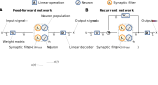
\includegraphics{media/chapters/01_introduction/ff_vs_rec_response_time_overlay.pdf}%
	\kern-158mm\includegraphics{media/chapters/01_introduction/ff_vs_rec_response_time.pdf}
	\caption[Neural networks can be faster than their fastest time-constant]{Neural networks can be faster than their fastest feed-forward time-constant. See \Cref{sec:nef,sec:temporal_tuning_lti} for more information.
	\textbf{(A)} Feed-forward computation with \SI{100}{\milli\second} first-order low-pass filters (\emph{synaptic filters}) in its forward path. Sending a pulse signal $u(t)$ into this network, we receive a low-pass filtered output $x(t)$ that \emph{slowly} converges to $u(t)$.
	\textbf{(B)} By adding recurrent connections and solving for weight matrices $\mat W$, $\mat W_\mathrm{rec}$, we can (in the limit of $n \to \infty$) realise any dynamical system, including low-pass filters with time-constant $t' < \tau$ (coloured lines;  cf.~\cite[Chapter~8]{eliasmith2003neural}).
	}
	\label{fig:ff_vs_rec_response_time}
\end{figure}

\begin{table}[p]
	\small\sffamily
	\centering
	\caption[Comparison between spatial and spatiotemporal computation]{Comparison between spatial and spatiotemporal computation. Spatial (static, or non-temporal) computation can be modelled as a first-order functions $f$, spatiotemporal computation relies on second-order functions processing the entire input history $\mathfrak{x}(t)$ for $t \leq 0$.
	Listed are the resources used to establish the function basis, i.e., tuning curves, in neural networks (see also \Cref{chp:temporal_tuning}).
	}
	\label{tbl:spatiotemporal}
	\begin{tabular}{r p{5.9cm} p{5.9cm}}
		\toprule
		& \textbf{Spatial computation} & \textbf{Spatiotemporal computation} \\
		\cmidrule(l){2-2}\cmidrule(l){3-3}
		&  $\begin{aligned} f: \mathbb{R}^d &\longrightarrow \mathbb{R}^{d'} \\ f(\vec x) &\mapsto \vec y \end{aligned}$ & $\begin{aligned} f : (\mathbb{R}^- \longrightarrow \mathbb{R}^d) &\longrightarrow \mathbb{R}^{d'} \\ f(\mathfrak{x}) &\mapsto \vec y\end{aligned}$ \\
		\cmidrule{1-1}\cmidrule(l){2-2}\cmidrule(l){3-3}
		\textit{Domain} & Input $\vec x \in \mathbb{R}^d$ & Signal $\mathfrak{x} \in \{ f \mid f : \mathbb{R}^- \longrightarrow \mathbb{R}^d) \}$ \\
		\cmidrule{1-1}\cmidrule(l){2-2}\cmidrule(l){3-3}
		\textit{Codomain} & Output $\vec y \in \mathbb{R}^{d'}$ & Output $\vec y \in \mathbb{R}^{d'}$ \\
		\cmidrule{1-1}\cmidrule(l){2-2}\cmidrule(l){3-3}
		\textit{Function basis} & Tuning curves $a_i(\vec x)$ & Temporal tuning curves $a_i(\mathfrak{x})$ \\
		\cmidrule{1-1}\cmidrule(l){2-2}\cmidrule(l){3-3}
		\textit{Neural resources}  & \textbullet\ Somatic \& dendritic nonlinearities & \textbullet\ Somatic \& dendritic nonlinearities \\
		                  & & \textbullet\ Synaptic filters \& axonal delays \\
		                  & & \textbullet\ Intrinsic dynamics \\
		                  & & \textbullet\ Recurrent connections \\
		\bottomrule
	\end{tabular}
\end{table}

While it is undisputed that dynamics play an important role in the brain, there are few \emph{overarching} theories that suggest how dynamics should be integrated into models of biological and cognitive systems.
Cybernetics \citep{wiener1948cybernetics} and dynamicism \citep{vangelder1998dynamical,eliasmith1996third} stand out as attempts to establish dynamics-focused research programs, but, as of writing, have either been subsumed by other fields or faded to obscurity.
Instead, the temporal evolution of biological and cognitive systems are modelled, often separately, at every possible level of abstraction---from individual neurons and their subcomponents \citep[e.g.,][]{gerstner2002spiking,izhikevich2007dynamical}, over small- and large-scale networks \citep[e.g.,][]{gerstner2014neuronal,bassett2017network}, to behaviour and language \citep[e.g.,][]{anderson1997actr,debot2007dynamic}.

What is missing are \emph{bridging laws}, that describe in broad strokes how low-level mechanism gives rise to high-level behaviour and cognition.
Building upon earlier work by \citet{eliasmith2003neural}, this thesis is an attempt at providing such laws.

In particular, our goal is to study ways in which low-level neural dynamics can be harnessed as a resource for high-level function.
We approach this from two different directions.
First, we analyse the dynamics intrinsic to passive dendritic trees, and derive a static model of dendritic nonlinearity that can be systematically exploited for high-level, non-temporal computation.
Second, we investigate \enquote{temporal tuning} as a low-level characterisation of individual model neurons.
This allows us to construct networks that can approximate arbitrary spatiotemporal functions (cf.~\Cref{tbl:spatiotemporal}), while outperforming common methods from machine learning.

Importantly, we focus on being as integrative as possible.
That is, our goal is \emph{not} to model biological phenomena at the greatest possible detail, but to think about mathematically tractable ways in which a broad range of neurophysiological and behavioural phenomena can be captured.
This way, we hope to provide a useful tool for researchers wishing to model high-level function, while constraining their work to physiological data.

Similarly important, and returning to our comparison between brains and computers, our approach is not only useful for cognitive modellers, but also for scientists working on brain-inspired computers (so called \emph{neuromorphic hardware}), and to the field of machine learning.
Systematically thinking about ways in which the computational substrate connects to function informs both the architecture of neuromorphic computers, and suggests a \enquote{neural compiler} for realising desired algorithms on these devices \citep{boahen2017neuromorph,voelker2021programming}.
Furthermore, our approach lends itself to thinking about the \enquote{best possible} representation that should be established in a neural network, and can thus pave the way in which artificial neural networks that are faster to train, more data-efficient, and higher performing \citep{voelker2019lmu,chilkuri2021parallelizing}.

\subsubsection{Structure and overview of this thesis}

The remainder of this thesis is structured as follows.
In \Cref{chp:modelling_neurobiological_systems} we review the aforementioned techniques for modelling and simulating neurobiological systems.
For readers with a mathematical, but no further biology background, we first introduce fundamental concepts from neuroscience, and then discuss our main modelling technique, the \emph{Neural Engineering Framework} (\NEF; \cite{eliasmith2003neural}).
We close with a discussion of shortcomings of the \NEF that we hope to resolve in this thesis.

We continue in \Cref{chp:nlif} by describing novel methods for integrating complex neuron models with multiple input channels and conductance-based synapses into \NEF networks.
Specifically, we focus on a mathematically tractable extension to the \LIF neuron, namely the $n$-compartment \LIF, or \nlif, neuron.
The purpose of this is twofold.
First, our extensions to the \NEF allow modellers to better constrain their models to neurophysiological data (we explore this in more detail in \Cref{chp:cerebellum}).
Second, we demonstrate---both in theory, and in simulation---that it is possible to systematically exploit the dynamics intrinsic to the passive dendritic tree of the \nlif neuron to perform multivariate, non-temporal computation in a spiking neural network context.
That is, \NEF networks with \nlif neurons can be made to automatically employ a simple form of \emph{dendritic computation} \citep{mel1994information,london2005dendritic} and to thus approximate a larger range of functions well compared to similar networks with standard \LIF neurons, and to even outperform two-layer networks.
In particular, we can model gain modulation, an important phenomenon in the central nervous system \citep{salinas2000gain,chance2002gain}.
Our results may inform the design of future and enable a better utilisation of existing neuromorphic computers.

Next, in \Cref{chp:temporal_tuning}, we introduce the notion of \emph{temporal tuning curves} to the \NEF.
Based on a model of spatiotemporal receptive fields in visual cortex \citep{carandini1999linearity}, temporal tuning curves provide a systematic way to compute functions \emph{through time} (\Cref{tbl:spatiotemporal}).
This approach is a generalisation of the \NEF dynamics principle, and a paradigm shift that offers a unified view onto resources for temporal computation, including synaptic filters, time-delays, and, to some degree, intrinsic neural dynamics.

Interestingly, we can, with small modifications, reuse a convex optimisation problem derived in the previous chapter to solve for weights that realise desired temporal tuning.
The weight solving procedure does not distinguish between feed-forward and feedback connections, and we can employ feedback connections to realise diverse temporal tuning.
Building upon previous work by \citet{voelker2018improving}, we show that mapping linear time-invariant (\LTI) systems approximating sliding-window transformations onto spiking neural networks generates temporal tuning that resembles time cells \citep{pastalkova2008internally,howard2014unified,tiganj2016sequential}.
We present a general method for constructing such \LTI systems.

Interestingly, our spatiotemporal \NEF populations are equivalent to a layer of Legendre Memory Units (\LMUpl; \cite{voelker2019lmu}).
\LMUpl are an exciting artificial neural network architecture for stream-to-stream processing.
We find evidence that one of our \LTI systems may possess more favourable computational properties compared to the standard \LTI system used in the \LMU, while offering a higher performance in some experiments.

As a final experiment in \Cref{chp:cerebellum}, we combine the approaches outlined in the previous chapters to construct an adaptive filter model of the cerebellum \citep{fujita1982adaptive}.
We apply our methods for constraining \NEF networks to more biological constraints (including Dale's principle; cf.~\Cref{chp:nlif}) to the recurrent Granule-Golgi circuit.
This circuit can in principle implement an \LTI system generating a temporal basis as discussed in \Cref{chp:temporal_tuning}.
Building upon the Granule-Golgi circuit we constrcut a network that can learn to decode arbitrary delays, reproducing basic features of eyeblink conditioning \citep[e.g.,][]{heiney2014cerebellardependent}.

We conclude with a short discussion of our contributions and potential future work in \Cref{chp:conclusion}.
Proofs and additional information may be found in \Cref{app:math_detail,app:data}, and an overview the software written for this thesis, namely \emph{libnlif} and \emph{NengoBio} in \Cref{app:software}.

\begin{FloatingBox}{Notational conventions}
\setlength{\parskip}{0.5em}
Some effort has been made to be as consistent as possible in the mathematical notation.
Bold lower-case letters (e.g., $\vec x$, $\vec \gamma$) denote vectors, while bold upper-case letters (e.g., $\mat X$, $\mat \Gamma$) denote matrices.
Double-struck letters denote sets, with $\mathbb{N}$, $\mathbb{Z}$, $\mathbb{Q}$, $\mathbb{R}$, $\mathbb{C}$ being our usual number systems.

We generally assume that vectors are column vectors, i.e., $\vec x \in \mathbb{R}^d$ is implicitly a matrix $\vec x \in \mathbb{R}^{d \times 1}$.
Correspondingly, $\vec x^T \vec y =  \langle \vec x, \vec y \rangle$ forms an inner product, and $\vec x \vec y^T = \vec x \otimes \vec y$ is an outer product.

When describing an entry in the $i$th row and the $j$th column of a matrix $\mat M$, we write $( \mat M )_{ij}$; $(\mat M)_i$ corresponds to the $i$th row, whereas $(\mat M^T)_j$ corresponds to the $j$th column.
All indices start with one.

We use the standard notation for the $L^p$ vector norm and the Frobenius matrix norm. Let $\vec x = (x_1, \ldots, x_d)$ and $\mat M \in \mathbb{R}^{m \times n}$ with $(\mat M)_{ij} = m_{ij}$. Then
\begin{align*}
	\|\vec x\|_0 &= | \{ x_k | x_k \neq 0 \} | \,, & 
	\|\vec x\|_p &= \sqrt[p\,\,]{\sum\nolimits_{k=1}^d |x_k|^p } \,, &
	\|\vec x\|_\infty &= \max\{ x_1, \ldots, x_d\} \,, &
	\| \mat M \|_\mathrm{F} = \sqrt{\sum\nolimits_{i=1}^m \sum\nolimits_{j=1}^n m_{ij}^2} \,\,.
\end{align*}
We define the inner product $\langle f, g \rangle$ and the convolution $f \ast g$ of two functions $f, g : \mathbb{R} \longrightarrow \mathbb{R}$ as
\begin{align*}
	\langle f, g \rangle &= \int_{-\infty}^\infty f(\tau) g(\tau) \,\mathrm{d}{\tau} \,, & 
	(f \ast g)(t) &= \int_{-\infty}^\infty f(t - \tau) g(\tau) \,\mathrm{d}{\tau} \,.
\end{align*}
\end{FloatingBox}

%
%	\setcounter{chapter}{1}
%	% !TeX spellcheck = en_GB

\chapter{Modelling Neurobiological Systems}
\label{chp:modelling_neurobiological_systems}

\begin{OpeningQuote}
First, it is an overstatement to describe what I am attempting here as an \enquote{approach toward the understanding}; it is merely a somewhat systematized set of speculations as to how such an approach ought to be made. That is, I am trying to guess which of the---mathematically guided---lines of attack seem, from the hazy distance in which we see most of them, a priori promising, and which ones have the opposite appearance.
\OpeningQuoteSource{John von Neumann}{The Computer and the Brain (1958)}
\end{OpeningQuote}

\begin{PriorPublication}
Parts of this chapter, particularly \Cref{sec:nef}, are based on \citet{stoeckel2021}.
Some figures in this chapter were adapted from material previously prepared for the University of Waterloo course SYDE 556/720, \enquote{Simulating Neurobiological Systems} taught by the author in winter 2020.
\end{PriorPublication}

% !TeX spellcheck = en_GB

The desire to understand cognition is by no means a new one---wondering about one's own thought processes has surely been part of the human condition since prehistoric times.
Today, we know that nerve cells in the brain are the primary functional and structural units that give rise to biological cognition.
This is referred to as the \emph{neuron doctrine}, a view that garnered support through observations made by Santiago Ramón y Cajal and Charles Scott Sherrington at the turn of the nineteenth century \citep[Chapter~2]{yuste2015neuron,bear2016neuroscience}.

Although the nature of neurons as independent units is undisputed, the neuron doctrine continues to be scrutinised.
There is an argument to be made that neural circuits are better described from the perspective of neural ensembles instead of individual neurons \citep{yuste2015neuron,churchland1992computational}---an idea that we revisit in the context of population codes.
Furthermore, it is still a matter of debate in how far structures such as Glial cells, must be taken into account to accurately model brain function \citep[e.g.,][]{verkhratsky2000ion}.

\begin{figure}
	\centering
	\includegraphics{media/chapters/02_modelling/02_00/levels.pdf}
	\caption[Illustration of temporal and spatial scales in neuroscience]{Illustration of temporal and spatial scales in neuroscience. Placement of individual concepts is deliberately coarse and, in some cases, open to debate. Spatial scale and levels of organisation adapted from \citet[Figure~1.4, p.~11]{churchland1992computational}.
	Temporal scales inspired by \citet[Figure~1]{sejnowski2014putting}.
	}
	\label{fig:spatial_and_temporal_scales}
	\vspace*{-0.5em}
\end{figure}

The fact that,  after more than a century of research, such fundamental debates still persist, illustrates that neuroscience (and by extension the other cognitive sciences) are still in their early days.
This is not due to a lack of talent or dedication;
rather, the gaps in our knowledge are a testament to the intrinsic difficulty of understanding complex systems such as the brain.

In some regard, neuroscience may be compared to physics.
Both fields study and predict the behaviour of natural systems, and both study phenomena that span vast spatial and temporal scales
(cf.~\Cref{fig:spatial_and_temporal_scales}).
Unlike physics, neuroscience is concerned with the behaviour of living objects consisting of billions of complex elements.%
\footnote{The human brain has $67$-$86\times10^{9}$ neurons and $\sim$$85\times10^9$ glial cells \citep{vonbartheld2016search}. Each neuron in cerebral cortex possesses $10^3$-$10^4$ synapses \citep[Chapter~6]{braitenberg2013anatomy}.}
The evolved nature of brains in particular makes it challenging to disentangle structures merely responsible for metabolic function, from those orchestrating behaviour.
Therefore, as demanded by many in the field \citep[e.g.,][]{marr1982vision,churchland1992computational,eliasmith2003neural}, neuroscience should be guided by predictive computational modelling and theory.%, with the goal to systematically connect mechanisms to behaviour, and to abstract unnecessary detail.

Here, the term \enquote{theory}, refers to overarching concepts applicable to different models \citep[e.g.,][]{stevens2000models}.
Continuing our physics analogy, successful physical theories such as Newtonian or Lagrangian mechanics, describe phenomena at different scales---from falling apples to solar systems orbiting their galactic centre.
Translating this to neuroscience, we would like our theories to connect low-level mechanisms (e.g., neurons, synapses, action potentials) to high-level behaviour (e.g.,~motor control, decision making, language).
As of now, there is no widely accepted theory that accomplishes this \citep[Chapter~9]{eliasmith2013how}.

All this is not to say that neuroscience has stagnated over the past decades.
To the contrary.
New recording methods---such as fMRI (functional magnetic resonance imaging), high-density multi-electrode arrays, calcium imaging, and optogenetics---have widened our perspective on brain function \citep{sejnowski2014putting}. Researchers have mapped out individual brain circuits \citep[e.g.,][]{shepherd2012handbook}, can describe neurons at a molecular level \citep[e.g.,][]{sobolevsky2009xray}, and determined the roles specific brain regions play in cognition \citep[e.g.,][]{kanwisher2006fusiform}.

Paradoxically, recent progress in neuroscience has made finding theories that bridge multiple levels of analysis \emph{more}, and not less important.
The central challenge is that each dataset on its own is fairly limited, mostly because different recording techniques possess dissimilar temporal and spatial characteristics \citep{sejnowski2014putting}.
The data we have access to is not detailed enough to directly inform large-scale models, and our theories are not sophisticated enough to combine heterogneous datasets. As pointed out by \citet{churchland1992computational}, there is an argument to be made that neuroscience has been, and still is, \enquote{data poor \emph{and} theory poor}.
A major difficulty in modelling brain function hence lies in building models that can be constrained by, and that make predictions compatible with, the different scales at which current recording techniques operate \citep[Chapter~9]{eliasmith2013how}.

As of now, there are a few attempts at developing such theories, or, less ostentatiously, \emph{modelling frameworks}, that facilitate describing the nervous systems at different scales.
Examples include the Neural Engineering Framework (\NEF; \cite{eliasmith2003neural}), Efficient, Balanced Spiking Networks (\EBN; \cite{boerlin2011spikebased,boerlin2013predictive}), and, to some degree, FORCE~\citep{sussillo2009generating,nicola2017supervised}.
Generally speaking, these approaches describe how to translate dynamical systems---corresponding to some hypothesized behavioral model---into an idealized spiking neural network that adheres to desired neurophysiological constraints.
Depending on the specific method, this can include neural tuning, firing rate distributions, and population-level connectivity~\citep{komer2016unified,nicola2017supervised}.
The resulting networks can then be analysed using the same techniques as biological systems, bridging the gap between empirical data and theory.

As we mentioned in \Cref{chp:introduction}, a goal of this thesis is to extend the Neural Engineering Framework to better take mechanistic constraints often found in the neuroscience literature into account.
To this end, we first review fundamental neuroscientific concepts, and then describe the \NEF along with list of biological constraints currently not well-captured by the \NEF.
We then, in subsequent chapters, propose extensions to the \NEF that, to some degree, alleviate these issues.
Finally, we demonstrate constructing a detailed biological of eyeblink conditioning in the cerebellum.


\clearpage
\setcounter{section}{0}
% !TeX spellcheck = en_GB

\section{Morphology and Physiology of Individual Neurons}
\label{sec:neurophysiology}

\begin{figure}
	\centering
	{\phantomsubcaption\label{fig:neuron_sketches_motor}}%
	{\phantomsubcaption\label{fig:neuron_sketches_pyramidal}}%
	{\phantomsubcaption\label{fig:neuron_sketches_purkinje}}%
	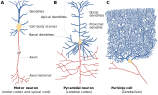
\includegraphics{media/chapters/02_modelling/02_01/neuron_sketches.pdf}
	\caption[Drawings of neurons in different brain regions]{Drawings of neurons in different brain regions.
	Although key structural elements can be identified across neurons, they can have very different morphologies.
	Redrawn from Ramón y Cajal.
	Overall presentation from \citet{kandel2012principles}, Figure~2-3D, p.~25.
	\textbf{(A)} Schematic drawing of a motor neuron (\cite{ramonycajal1894nouvelles}, Figure 6, p.~25).
	\textbf{(B)} Human cortical pyramidal neuron (\cite{howell1916textbook}, Figure~84, p.~187).
	\textbf{(C)} Human purkinje cell in the cerebellum (\cite{ramonycajal1909histologie}, Figure~9, p.~61).
	\label{fig:neuron_sketches}
	}
\end{figure}

Neurons come in various sizes, shapes, and degrees of interconnectedness.
Ramón y Cajal's\index{Ramón y Cajal, Santiago} drawings (schematically redrawn in \Cref{fig:neuron_sketches}) offer a glimpse of the morphological diversity found in the nervous system.
Some neurons possess only few branches (also \emph{projections}\index{neuron!projection}) and have a comparably simple structure, whereas others, such as Cerebellar Purkinje cells, feature sprawling dendritic trees more deserving of the name \enquote{dendritic forest}.

It should come as no surprise that the following review of neural morphology and physiology cannot do justice to the incredible complexity observed in nature.
Our goal is to instead focus on structural and functional elements commonly observed across all neurons.
As a side-effect, the resulting characterisation of the nervous system lends itself well to computational models.
%While the simplifications we make come at the risk of ignoring details that could turn out to be essential for modelling brain function, some simplification
%Yet, as discussed above, we would like to develop theories that bridge as many levels of scale as possible.
%The aspects of biology that we incorporate into our models are known to play a major role in overall brain function.
We open with a high-level overview of neural function and structure, and then focus on aspects of neural electrophysiology that will be relevant in later sections, including the generation of the membrane potential, action potentials, and synaptic transmission.
Readers interested in a more thorough introduction to neuroscience are encouraged to consult neuroscience textbooks such as \citet{bear2016neuroscience}, \citet{purves2017neuroscience}, or \citet{kandel2012principles}.

\subsection{Functional and Structural Overview}
\label{sec:neurons_overview}

\begin{figure}
	\centering
	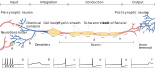
\includegraphics{media/chapters/02_modelling/02_01/neuron_signals_overview.pdf}
	\caption[Overview of neural function]{Overview of neural function. Inset diagrams illustrate the membrane potential over time at the indicated locations (data from a compartmental Hodgkin-Huxley-type model neuron). Arrows indicate the predominant flow of information. \emph{Input:} Neurons receive signals from pre-synaptic neurons through synapses. For chemical synapses, action potentials (\enquote{spikes}) arriving at the synapse (\emph{a}) cause a release of neurotransmitter that induces a post-synaptic potential (PSP) in the post-synaptic neuron (\emph{b}). \emph{Integration:} PSPs from multiple pre-synaptic neurons interact in the dendrites. Under certain conditions the neuron produces its own action potential (\emph{c}). \emph{Conduction:} The action potential travels along the axon (\emph{d}-\emph{e}). \emph{Output:} The neuron induces a PSP in a post-synaptic neuron (\emph{f}).
	}
	\label{fig:neuron_signal_overview}
\end{figure}

From the perspective of computer science---and as suggested by the neuron doctrine---neurons are fundamental units of computation in biological systems.
Specifically, neurons employ weak bioelectric signals, variations in their membrane potential, to compute.
As depicted in the lower portion of \Cref{fig:neuron_signal_overview}, these variations can either be gradual, as is the case when the neuron is in its \emph{subthreshold} regime\index{membrane potential!subthreshold}, or manifest themselves as rapid swings between the highest and lowest voltages that can be produced by a neuron; in this case the neuron is in its \emph{superthreshold} regime.
These rapid voltage changes are called \emph{action potentials}\index{action potential}, or, more colloquially, \enquote{\emph{spikes}}, harking back to their prominent appearance on oscillograms.
% TODO: Index: spike -> action potential

Typically, gradual subthreshold potentials are not directly accessible from other parts of the network;
this analogue code is solely part of a neuron's internal state.
Hence, from the perspective of other neurons in the network, a neuron is either \enquote{silent} or \enquote{spiking}.
This binary nature of neurons fascinated early computer scientists such as \citet{vonneumann1958computer}\index{Von Neumann,John} and led to the development of the first artificial neural networks by \citet{mcculloch1943logical}.

Neuroscientists typically divide neural information processing into four stages: input, integration, conduction, and output \citep[Chapter 2]{kandel2012principles}.
These stages roughly correspond to different features of neural structure, as depicted in \Cref{fig:neuron_signal_overview}.

The \emph{input region} corresponds to the dendrites, and the synapses embedded therein.%
\footnote{
The difference between input and output regions of a neuron is not always clear-cut.
Invertebrate unipolar cells only possess a single branch that protrudes from the cell body.
This branch is referred to as \enquote{axon} although it carries both input and output \citep[Chapter~2]{kandel2012principles}.}
Dendrites are tree-like structures protruding out of the cell body, typically less than two millimetres long \citep[Chapter~1]{bear2016neuroscience}.
They are usually classified according to their location relative to the cell body.
For example, in pyramidal cells (cf.~\Cref{fig:neuron_sketches_pyramidal}) dendrites directly connected to the soma are called \emph{basal}\index{dendrite!basal^}; dendrites indirectly connected to the soma through longer projections are called \emph{apical}\index{dendrite!apical}.
Apical dendrites are sometimes additionally divided---using standard anatomical terminology---into parts referred to as \emph{proxmial} or \emph{distal}; that is, they are either closer or father away from the soma \citep[e.g.,][Figure~5]{seamans1997contributions}.

Synapses form the coupling sites between neurons and---in the case of chemical synapses discussed below---establish a unidirectional flow of information.
This ensures that pre-synaptic neurons only influence the state of the post-synaptic neuron, but not vice-versa \citep[Chapter~8]{kandel2012principles}.
Some neurons in the periphery of the nervous system act as sensors; they transduce modalities such as temperature, pressure or light and do not rely on synaptic inputs \citep[Chapter~22]{kandel2012principles}.

The neuron's \emph{integration region} is formed by the cell body and, to some degree, the dendritic tree itself.
Signals from several pre-synaptic neurons interact here.
This interaction may elicit the generation of an output signal.
As we mentioned before, this output takes the form of an \emph{action potential}\index{action potential} in most vertebrate neurons \citep[Chapter~2]{kandel2012principles}.
Crucially, and in contrast to artificial neural networks, the integration process has a temporal component; the input \emph{history} is relevant for the generation of the output, and not just the momentary input.

The \emph{conductive region} corresponds to a neuron's axon\index{axon}.
The axon carries signals generated by the neuron to other parts of the nervous system.
Two features of the axon work in tandem to ensure signal integrity \citep[Chapter~7]{kandel2012principles}.
First, the axon is electrically well insulated, being tightly wrapped in Schwann's cells\index{Schwann's cell}, a type of glial cell\index{glial cell}.
Second, axons actively renew action potentials at Nodes of Ranvier\index{Node of Ranvier}, gaps between neighbouring Schwann's cells.
Conduction is unidirectional in the sense that action potentials only travel away from the origin of excitation.
Notably, in larger animals such as humans, individual neurons conduct signals across micrometres (between neighbouring neurons), centimetres (connecting different parts of the brain), and metres (motor neurons in the spinal cord).%

Finally, the \emph{output region} corresponds to the area surrounding the synapses that lie between the axon terminals and post-synaptic dendrites.
In the case of chemical synapses, the arrival of an action potential at the axon terminal causes the release of neurotransmitter molecules.
Receptors in the post-synaptic neuron transduce neurotransmitters into an input signal, a post-synaptic potential.
In the periphery, axon terminals may be coupled to muscle fibres, where the arrival of an action potential generates movement \citep[Chapter~8~\&~9]{kandel2012principles}.

\subsection{Ion channels and the membrane potential}
\label{sec:membrane_potential}

\begin{figure}
	\centering
	{\phantomsubcaption\label{fig:neuron_membrane_potential_membrane}}%
	{\phantomsubcaption\label{fig:neuron_membrane_potential_membrane_isolated}}%
	{\phantomsubcaption\label{fig:neuron_membrane_potential_membrane_channel}}%
	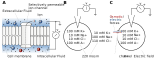
\includegraphics{media/chapters/02_modelling/02_01/neuron_membrane_potential.pdf}
	\caption[Membrane potential as a result of selectively permeable ion channels]{
	Membrane potential as a result of selectively permeable ion channels.
	\textbf{(A)} The cell membrane separates the intra- and extracellular fluid. Charge carriers (e.g., ions) are in solution in the fluids. The membrane potential is the voltage \vMem across the membrane.
	Specific ions may pass through selectively permeable channels.
	\textbf{(B)} If the membrane was a perfect insulator, there would be no membrane potential. Molar concentration in $\mathrm{mM} = \si{\milli\mole\per\litre}$; values illustrative. $A^-$ corresponds to charged anionic molecules.
	The individual fluids are electrically neutral.
	\textbf{(C)} Adding a selectively permeable ion channel results in a membrane potential specific to the ion species at which electric and osmotic forces cancel out.
	Illustrations (B, C) adapted from \citet{reichert2000neurobiologie}, Figures 2.8 and 2.10.}
\end{figure}

As mentioned above, neurons process information by systematically varying their membrane potential\index{membrane potential}\index{potential!membrane} \vMem (more precisely, their \emph{transmembrane} potential).
The membrane potential is the electrical potential between the inside and outside of a cell.
The boundary between these regions is formed by the cell membrane, a double-layer of lipids.%
\footnote{To be clear, \emph{all} biological cells possess bioelectrical properties, including a membrane potential.
This was for example analysed in detail by Julius Bernstein\index{Bernstein, Julius} in the early 1900s \citep{bernstein1912elektrobiologie}. Membrane potentials are important for homeostasis and cell-to-cell communication \citep{moorhouse2016membrane}.
For example, electrical gradients between cells are crucial for laying out the body plan of organisms \citep{levin2014molecular}.
Neurons should be thought of as cells shaped by evolution to excel at bioelectrical signalling, but are not unique in their use of bioelectricity.}
By convention, if the \emph{inside} is more positively charged than the outside, we report a positive voltage (\Cref{fig:neuron_membrane_potential_membrane}).

Measuring the membrane potential when a neuron is at rest---that is, when the cell does not receive any input---reveals the so-called resting potential \vRest.
In mammals, \vRest ranges from \SIrange{-50}{-85}{\milli\volt} depending on the cell type \citep{moorhouse2016membrane}.

Upon closer investigation, the presence of a non-zero resting potential is rather surprising.
The inside and outside of the cell are filled with watery solutions: the intracellular fluid (\enquote{cytoplasm}\index{cytoplasm}) and the extracellular fluid.
Both fluids are electrically neutral.
That is, although the fluids contain ions and anionic charge carriers in solution, the overall positive and negative charges are balanced.
There should be no measurable electrical potential (\Cref{fig:neuron_membrane_potential_membrane_isolated}).


\subsubsection{Selectively permeable ion channels generate the membrane potential}
\begin{figure}
	\centering
	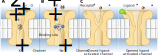
\includegraphics{media/chapters/02_modelling/02_01/channel.pdf}%
	{\phantomsubcaption\label{fig:ion_channels_k}}%
	{\phantomsubcaption\label{fig:ion_channels_na}}%
	{\phantomsubcaption\label{fig:ion_channels_gate}}%
	\caption[Schematic illustration of ion channels  embedded into the cell membrane]{Schematic illustration of ion channels embedded in the cell membrane. Ion channels are pores that selectively let ions of a certain species pass. Selectivity is achieved by exploiting the radius and charge distributions of the ion and its watery hull. \textbf{(A)} Although the $\mathrm{K^+}$ ion is larger than the $\mathrm{Na^+}$ ion, its watery hull is more compact, and it can pass through narrower channels. \textbf{(B)}  $\mathrm{Na^+}$ selectivity is achieved by a negative binding site in the channel that stabilises the $\mathrm{K^+}$ ion and its hull to let it pass.  \textbf{(C)} Ion channels can change their conformation depending on external factors (e.g.~mechanical forces, chemicals, electrical potentials); here, a chemical ligand opens a channel. Inspired by \citet[Figure~5-1, p.~102 and Figure~5-6, p.~109]{kandel2012principles}; see ibid.~for more information.}
\end{figure}
The resting potential can be explained if we assume that the cell membrane is selectively permeable to some ions through so-called \emph{ion channels}\index{ion channel}.
The presence of ion channels has been postulated for a long time, though it is only thanks to relatively recent studies that we understand the molecular machinery that underpins selective permeability \citep[Chapter~5]{kandel2012principles}.

Ion channels are porous proteins embedded in the cell membrane.
They accomplish the impressive feat of acting as an \enquote{atomic sieve}.
This \enquote{sieve} only lets a single ion of a certain kind (in chemical parlance: \emph{ion species}\index{ion species}) pass at a time, as is illustrated in \Cref{fig:ion_channels_k,fig:ion_channels_na}.
Furthermore, as we will see both in the context of action potential generation and synaptic transmission, these proteins can change their shape, or \emph{conformation}, depending on various external circumstances, effectively opening or closing the channel (\Cref{fig:ion_channels_gate}).

Of course, the mere presence of selectively permeable channels does not explain the membrane potential.
For this, we have to consider that despite being electrically neutral, the intra- and extracellular fluids contain different concentrations of the individual charge carriers.
In particular, there are large concentration gradients for potassium ($\mathrm{K^+}$), sodium ($\mathrm{Na^+}$) and chloride ($\mathrm{Cl^-}$) ions.
For example, the concentration of potassium ions $\mathrm{K^+}$ is about \SI{140}{\milli\mol\per\litre} in the cytoplasm, compared to \SI{3}{\milli\mol\per\litre} in the extracellular fluid.
If the cell membrane was permeable to $\mathrm{K}^+$ ions, an osmotic force would act on the ions, driving them outside.

This ionic flow disturbs the charge balance of the intra- and extracellular fluids and results in a non-zero membrane potential.
In turn, this potential results in an electric force that counters the osmotic pressure.
In our $\mathrm{K}^+$ example, the intracellular fluid becomes negatively charged and the ensuing electric attraction reduces the net force acting on the $\mathrm{K}^+$ ions.
The system converges to an equilibrium point where the electric and osmotic forces cancel out (\Cref{fig:neuron_membrane_potential_membrane_channel}).
The membrane potential at this point is called the \emph{equilibrium}\index{equilibrium potential}\index{potential!equilibrium} or \emph{reversal potential}\index{reversal potential}\index{potential!reversal}, as the ionic flow direction reverses at this point.
For clarity, we use the term reversal potential when talking about the equilibrium potential for a membrane permeable to a \emph{single} ion.


\subsubsection{A single selectively permeable ion channel: The Nernst equation}
For a single charge carrier $X$, the reversal potential $E_X$ can be computed using the Nernst equation\index{Nernst equation} \citep{nernst1888kinetik}:%
\footnote{The Nernst equation was published in 1888, before there were established theories about bioelectricity. Nernst studied the electrochemistry of electrolytes separated by membranes and this research was later incorporated into analyses of biological cell membranes by Ostwald and later Bernstein \citep[see][Chapter~5]{bernstein1912elektrobiologie}\index{Bernstein, Julius}.}
\newcommand{\Cout}[1]{\ensuremath{[\mathrm{#1}]_\mathrm{out}}}
\newcommand{\Cin}[1]{\ensuremath{[\mathrm{#1}]_\mathrm{in}}}
\begin{align}
	E_X &= -\frac{RT}{zF} \log \left( \frac{\Cin{X}}{\Cout{X}} \right) \,,
	\label{eqn:nernst}
\end{align}
where $R$ is the gas constant, $T$ is the temperature, $z$ is the charge number, or valence\index{valence}, of the particle (e.g., $z = 2$ for $\mathrm{Ca}^{2+}$ and $-1$ for $\mathrm{Cl}^-$) and $F$ is the Faraday constant. \Cout{X} and \Cin{X} are the concentrations (count per volume) of particles $X$ outside and inside the cell, respectively.
Note that the number of ions flowing through the cell membrane is rather minuscule compared to the total number of ions in solution; \Cout{X} and \Cin{X} essentially do not change over time.%
\footnote{The ion concentrations in the intra- and extracellular fluid are maintained by ion pumps in the cell membrane. These pumps are secondary for a cell's short-term bioelectrical properties, but are indispensible in the long run.}

\begin{table}
	\centering
	\caption[Ion concentrations and reversal potentials in the squid and mammals]{Ion concentrations and reversal potentials in the squid and mammals. Data from \citet[Table~12.1, p.~353]{mccormick2014membrane}. The squid data are based on \citet{hodgkin1949effect}, and reported similarly in \citet[Table~6-1, p.~128]{kandel2012principles}. Reversal potentials computed using \cref{eqn:nernst}.}
	\label{tbl:nernst}
	\small
	\sffamily
	\begin{tabular}{l l p{0.25cm} r r p{0.25cm} r r}
		\toprule
		&
		&
		& \multicolumn{2}{c}{\textbf{Concentrations}}
		&
		& \multicolumn{2}{c}{\textbf{Reversal potentials}} \\ %  \multicolumn{1}{c}{\textbf{Permeability ratios}}\\
		\cmidrule(lr){4-5}\cmidrule(lr){7-8}
		
		\multicolumn{2}{l}{\textbf{Ion species}}
		&
		& \emph{Intracellular}
		& \emph{Extracellular}
		&
		& $T = \SI{20}{\degreeCelsius}$
		& $T = \SI{36}{\degreeCelsius}$ \\ %& $P_\mathrm{K^+} : P_\mathrm{Na^+} : P_\mathrm{Cl^-}$ \\
		\midrule

		\multicolumn{2}{l}{\emph{Squid giant axon}}\\

		\raggedleft \quad Potassium
		& $\mathrm{K}^+$
		&
		& \SI{400}{\milli\mol\per\litre}
		& \SI{20}{\milli\mol\per\litre}
		&
		& \SI{-76}{\milli\volt}
		& \SI{-80}{\milli\volt} \\

		\raggedleft \quad Sodium
		& $\mathrm{Na}^+$
		&
		& \SI{50}{\milli\mol\per\litre}
		& \SI{440}{\milli\mol\per\litre}
		&
		& \SI{55}{\milli\volt}
		& \SI{58}{\milli\volt} \\

		\raggedleft \quad Chloride
		& $\mathrm{Cl}^-$
		&
		& \SI{40}{\milli\mol\per\litre}
		& \SI{560}{\milli\mol\per\litre}
		&
		& \SI{-67}{\milli\volt}
		& \SI{-70}{\milli\volt} \\[0.25cm]

		\multicolumn{2}{l}{\emph{Mammalian neuron}}\\

		\raggedleft \quad Potassium
		& $\mathrm{K}^+$
		&
		& \SI{140}{\milli\mol\per\litre}
		& \SI{3}{\milli\mol\per\litre}
		&
		& \SI{-97}{\milli\volt}
		& \SI{-102}{\milli\volt} \\

		\raggedleft \quad Sodium
		& $\mathrm{Na}^+$
		&
		& \SI{18}{\milli\mol\per\litre}
		& \SI{145}{\milli\mol\per\litre}
		&
		& \SI{53}{\milli\volt}
		& \SI{56}{\milli\volt} \\

		\raggedleft \quad Chloride
		& $\mathrm{Cl}^-$
		&
		& \SI{7}{\milli\mol\per\litre}
		& \SI{120}{\milli\mol\per\litre}
		&
		& \SI{-72}{\milli\volt}
		& \SI{-76}{\milli\volt} \\

		\bottomrule
	\end{tabular}
\end{table}

\subsubsection{Multiple selectively permeable ion channels: The Goldman-Huxley-Katz equation}
\Cref{tbl:nernst} lists the ion concentrations of the squid giant axon---a model system common in the early days of neuroscience---as well as mammalian cells.
Although there are large differences in the ion concentrations, the reversal potentials (when computed using eq.~\ref{eqn:nernst}) are similar across species.
Still, we find that, in general, no individual reversal potential exactly matches the resting potential.
For example, in the squid, the resting potential is close to \SI{-62}{\milli\volt} at a temperature of \SI{20}{\degreeCelsius} (\cite{mccormick2014membrane}).
This potential is slightly more positive than $E_\mathrm{K^+}$ and $E_\mathrm{Cl^-}$, but much more negative than $E_\mathrm{Na^+}$.

This suggests that the cell membrane is permeable to several ion species at the same time, but at different \enquote{permeabilities}.
The membrane potential converges to a new equilibrium state $E$ somewhere between the original reversal potentials.
Mathematically, we summarise the relative permeability of the cell membrane for an ion species $X$ as a quantity $P_X$.
Instructively, $P_X$ can be interpreted as the total number of open ion channels for an ion species $X$.

We can compute the overall equilibrium potential using the Goldman-Huxley-Katz equation\index{Goldman-Huxley-Katz equation} \citep{goldman1943potential,hodgkin1949effect}.
For the three ion species listed above we have
\begin{align}
	E &= \frac{RT}{F} \log \left( \frac{
		P_\mathrm{K^+} \Cout{K^+} +
		P_\mathrm{Na^+} \Cout{Na^+} +
		P_\mathrm{Cl^-} \Cin{Cl^-}}{
		P_\mathrm{K^+} \Cin{K^+} +
		P_\mathrm{Na^+} \Cin{Na^+} +
		P_\mathrm{Cl^-} \Cout{Cl^-}
		} \right) \,.
	\label{eqn:goldman}
\end{align}
For the squid giant axon, the permeability ratios $P_\mathrm{K^+} : P_\mathrm{Na^+} : P_\mathrm{Cl^-}$ can be experimentally determined to be about $1: 0.04 : 0.45$---in its resting state, the membrane is strongly permeable to potassium, but only weakly so for sodium \citep{mccormick2014membrane}.
Plugging these numbers into \cref{eqn:goldman} results in the resting potential $\vRest \approx \SI{-62}{\milli\volt}$.

\subsubsection{Equivalent circuit model}
\begin{figure}
	\centering
	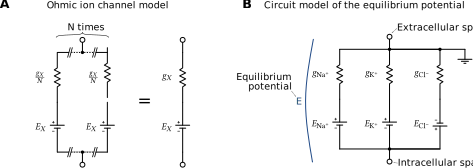
\includegraphics[scale=0.3333]{media/chapters/02_modelling/02_01/electrical_circuit.pdf}
	{\phantomsubcaption\label{fig:electrical_circuit_individual_channels}}
	{\phantomsubcaption\label{fig:electrical_circuit_membrane}}
	\caption[Electrical circuit model of the cell membrane]{Electrical model circuit of the cell membrane.
	\textbf{(A)} Individual ion channels can be modelled as a resistor-voltage-source pair (\emph{left}).
	Instead of modelling all ion channels for the same ion species $X$ independently, they can be mathematically combined into a single pair (\emph{right}).
	\textbf{(B)} Circuit model of a neuron at rest. The ratios of the conductances $g_\mathrm{K^+}$, $g_\mathrm{Na^+}$, and $g_\mathrm{Cl^-}$ determine the cell's equilibrium potential $E$. Arrows indicate the current direction relative to $E = \SI{0}{\volt}$ (not physical ionic flow).}
	\label{fig:electrical_circuit}
\end{figure}
Alternatively, the equilibrium potential can be modelled in terms of the equivalent circuit depicted in \Cref{fig:electrical_circuit}.
The idea is the following.
An ion species $X$ is \enquote{driven} by the voltage difference between the membrane potential \vMem and the reversal potential  $E_X$ (eq.~\ref{eqn:nernst} and \Cref{tbl:nernst}).
Each ion channel provides a conductive path for a specific ion species $X$; however, the channels are tiny, and ionic movement is influenced by thermal Brownian noise.
Hence, there is a chance that ions will collide with the cell interior before passing through a channel.
This provides a resistance $R_X$ to the ionic current \citep{enderle2011bioelectric}.

Each ion channel can thus be modelled electrically as a resistor-voltage-source pair.
The voltage source corresponds to the driving forces that move ions in or out of the cell, whereas the resistor models the stochastic resistance ions encounter while moving through the cell.

Intuitively, the more ion channels that are open---and the larger the permeability $P_X$---the smaller this resistance.
Assuming that $P_X$ represents the number of open channels for an ion species $X$, and that ion channels behave Ohmically, the total ionic current $J_X$ is  (\Cref{fig:electrical_circuit_individual_channels})
\begin{align}
	J_X(v) &= \sum_{i = 1}^{P_X} \frac{\vMem - E_X}{R_X} = \frac{P_X}{R_X} \bigl( \vMem - E_X \bigr) = g_X (\vMem - E_X)\,,
	\label{eqn:ionic_current}
\end{align}
where $g_X$ is the \emph{conductance} of a \enquote{virtual} channel summarizing all $P_X$ channels.%
\footnote{The conductance\index{conductance} $g$ of a resistor (measured in Siemens\index{Siemens}; unit symbol $\si{\siemens} = \si{\per\ohm}$) is the inverse of its resistance $R$.
This unit is commonly used in neuroscience to simplify some equations.
For example, a conductance of zero can be used to describe an open circuit, whereas resistances would take on unwieldy infinite values in this case.}
To obtain the equilibrium potential $E$ for multiple ion channels, we arrange the resistor-voltage-source pairs in parallel (\Cref{fig:electrical_circuit_membrane}).
According to Kirchoff's circuit laws\index{Kirchoff's circuit laws} we have
\begin{align}
	\sum_X J_X(E) = \sum_X g_X (E - E_X) &= 0 \Leftrightarrow E = \frac{\sum_X g_X E_X}{\sum_X g_X} \,, \quad \quad \text{for } \sum_X g_X > 0 \,.
	\label{eqn:circuit_equilibrium}
\end{align}
And for the ion species discussed above we get
\begin{align}
	E &= \frac{g_\mathrm{K^+} E_\mathrm{K^+} + g_\mathrm{Na^+} E_\mathrm{Na^+} + g_\mathrm{Cl^-} E_\mathrm{Cl^-}}{g_\mathrm{K^+} + g_\mathrm{Na^+} + g_\mathrm{Cl^-}} \,,  \quad \quad \text{for } g_\mathrm{K^+} + g_\mathrm{Na^+} + g_\mathrm{Cl^-} > 0 \,.
	\label{eqn:circuit_equilibrium_ions}
\end{align}
Put differently, the equilibrium potential is modelled as a weighted sum of reversal potentials, with the weights being the channel conductances.
However, note that \cref{eqn:ionic_current,eqn:circuit_equilibrium} assume a linear relationship between permeabilities and conductances.
Mathematically, conductance and permeability are two distinct concepts \citep{enderle2011bioelectric}.
Still, although linearity does not follow from the empirically well-tested Goldman equation, the linear approximation preserves the overall qualitative behaviour. We discuss this in more detail in \Cref{app:goldman_equiv_circuit_diff}.

Correspondingly, the above \enquote{equivalent circuit} forms the basis of most neuron models.
The model is simple, conductances can be fit to experimental data, and---as we will see next---the equivalent circuit lends itself to a dynamical description of the cell membrane by simply adding a capacitor to the model circuit.

\pagebreak

\subsection{Neural Dynamics and the Hodgkin-Huxley Model}
\label{sec:neural_dynamics}

We can now describe the steady-state membrane potential of a neuron at rest.
However, the mechanisms discussed so far neither tell us how the membrane potential evolves over time, nor do they describe the action potential---the phenomenon distinguishing most neurons from other cells in the first place.

Fundamentally, neural dynamics can be summarised as follows.
Assume that we inject short positive current pulses $J(t)$ into a neuron using a microelectrode.
Measuring the membrane potential $\vMem(t)$ over time $t$ we observe the following:
\begin{enumerate}[1.]
	\setlength{\itemsep}{0.25em}
	\vspace*{-0.25em}
	\item \emph{Subthreshold dynamics.} Small current pulses charge the cell membrane over time. The membrane potential \vMem rises while the input persists, and then decays back to \vRest (\Cref{fig:action_potentials_subthreshold}).
	\item \emph{Superthreshold dynamics.} If the current pulse is energetic enough for the membrane potential to reach a soft threshold value $v_\mathrm{th}$, the neuron generates an action potential; \vMem suddenly rises towards positive numbers (\emph{depolarisation}\index{neuron!depolarisation}), and then falls to voltages below \vRest (\emph{repolarisation}\index{neuron!repolarisation})---the neuron is \emph{hyperpolarised}\index{neuron!hyperpolarisation}. Over time, \vMem converges back to  \vRest.  This is depcited in \Cref{fig:action_potentials_superthreshold}.
	\item \emph{Refractory period.} While the neuron is hyperpolarised, it is significantly harder to evoke another action potential. This phase is referred to as the \emph{refractory period}\index{neuron!refractory period} (\Cref{fig:action_potentials_refractory}).%
	\footnote{Technically, modellers distinguish between \emph{absolute} and \emph{relative} refractory periods. During the absolute refractory period the neuron cannot produce action potentials; during the relative refractory period merely large input currents are required \citep[Section~2.3.2]{izhikevich2007dynamical}.}
\end{enumerate}

\vspace*{-0.25em}
The first model to provide a detailed mechanistic account of these observations---and indeed what we used as a stand-in for a real neuron in the above exploration---is the Hodgkin-Huxley model \citep{hodgkin1952quantitative}.
This model has been exceptionally successful in predicting neural behaviour quite accurately, and forms a basis for a whole family of neuron models \citep{meunier2002playing,mccormick2007hodgkin}.

The important idea of Hodgkin-Huxley-type models is that the channel conductances $g_\mathrm{K^+}$ and $g_\mathrm{Na^+}$ possess dynamics that nonlinearly depend on the current membrane potential.%
\footnote{Hodgkin-Huxley-type models are sometimes also called \enquote{conductance-based neurons}. This is not to be confused with \enquote{conductance-based synapses}---synapse models are independent of the neuron model.}
That is, the permeability of the membrane for potassium and sodium changes depending on the membrane potential due to voltage-dependent ion channels.
Hodgkin and Huxley model the dynamics of these channels using three dimensionless \enquote{gating} variables $m(t)$, $h(t)$, $n(t)$.
Revised models differ from the original in terms of the concrete dynamics of these variables.
In our examples, we use dynamics adapted from a model of pyramidal cells in the hippocampus described by \citet[Chapter~4, pp.~92-94; \Cref{app:hippocampal_hh}]{traub1991neuronal}.

\begin{figure}[p]
	\includegraphics{media/chapters/02_modelling/02_01/action_potentials.pdf}
	{\phantomsubcaption\label{fig:action_potentials_subthreshold}}
	{\phantomsubcaption\label{fig:action_potentials_superthreshold}}
	{\phantomsubcaption\label{fig:action_potentials_refractory}}
	\caption[Hodgkin-Huxley-type model neuron simulations demonstrating action potential generation]{Hodgkin-Huxley-type model neuron simulations demonstrating action potential generation (using the dynamics described by \cite{traub1991neuronal}).
	% This figure was in part inspired by \citet[Figure~2.15, p.~45]{izhikevich2007dynamical}
	\textbf{(A)} Injecting a current $J$ into the neuron (orange; \emph{bottom}) charges the cell membrane. As long as the membrane potential $v$ (\emph{top}) approximately stays below a threshold, the neuron does not generate action potentials; the membrane acts linearly. \textbf{(B)} Above a certain threshold, the neuron suddenly generates an action potential. \textbf{(C)} Directly after an action potential, during the \emph{refractory period}, even large input currents cannot evoke action potentials.}
\end{figure}

\begin{figure}[p]
	\vspace{0.5cm}
	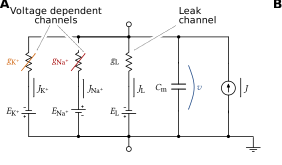
\includegraphics[scale=0.3333]{media/chapters/02_modelling/02_01/hodgkin_huxley_circuit.pdf}~~~~%
	\includegraphics{media/chapters/02_modelling/02_01/action_potentials_hh_conductances.pdf}
	{\phantomsubcaption\label{fig:action_potentials_hh_conductances_circuit}}
	{\phantomsubcaption\label{fig:action_potentials_hh_conductances_conductances}}
	\vspace{-0.5cm}
	\caption[Equivalent circuit diagram of the Hodgkin-Huxley model]{Equivalent circuit diagram of the Hodgkin-Huxley model. \textbf{(A)} Equivalent circuit model of the Hodgkin-Huxley model. The resting potential is generated by a virtual \enquote{leak} channel; the $\mathrm{K}^+$ and $\mathrm{Na}^+$ channels vary over time and depend on the membrane potential. \textbf{(B)} Conductance traces for a single action potential (slice from \cref{fig:action_potentials_superthreshold}). Sodium drives depolarisation, potassium repolarisation.}
	\label{fig:action_potentials_hh_conductances}
\end{figure}

Conveniently, Hodgkin-Huxley-type models are an extension of the equivalent cell-membrane circuit from the previous subsection (\Cref{fig:electrical_circuit}).
We just need to make two conceptual changes to account for the linear subthreshold and nonlinear superthreshold dynamics.

\subsubsection{Subthreshold dynamics}
To model the linear subthreshold dynamics, we simply add a capacitor with capacitance $C_\mathrm{m}$ to the circuit model.
This \emph{membrane capacitance}\index{neuron!membrane capacitance} is physically motivated by the cell membrane separating two electrically charged bodies.
Any such system inherently possesses capacitive properties.%
\footnote{To be clear, the membrane capacitance is not specific to the Hodgkin-Huxley model. In fact, this assumption preceded the Hodgkin-Huxley model by several decades (e.g., \cite{lapicque1907recherches}). We discuss the corresponding LIF neuron model first proposed by Lapicque later in this chapter.}
Given an input current $J(t)$, the sub-threshold dynamics can be described in terms of the following differential equation
\begin{align}
	\begin{aligned}
	\CMem \dot\vMem(t) &=
		  g_\mathrm{K^+} \bigl(E_\mathrm{K^+} - \vMem(t)\bigr)
		+ g_\mathrm{Na^+} \bigl(E_\mathrm{Na^+} - \vMem(t)\bigr)
		+ g_\mathrm{Cl^-} \bigl(E_\mathrm{Cl^-} - \vMem(t)\bigr) + J(t) \\ &=
	g_\mathrm{L} \bigl(\EL - \vMem(t)\bigr) + J(t) \,.
	\end{aligned}
\end{align}
The last term simplifies the dynamics using a \emph{leak conductance} \gL and \emph{leak potential} \EL that form a basic resistor-capacitance (RC) circuit (right half of \Cref{fig:action_potentials_hh_conductances_circuit}) with the time-constant $\tauMem = \CMem g_\mathrm{L}^{-1}$.
We have
\begin{align*}
	\gL &= g_\mathrm{K^+} + g_\mathrm{Na^+} + g_\mathrm{Cl^-} \,, &
	\text{and} \quad \quad \EL &= \frac{g_\mathrm{K^+} E_\mathrm{K^+} +
				 	g_\mathrm{Na^+} E_\mathrm{Na^+} + g_\mathrm{Cl^-} E_\mathrm{Cl^-}}{g_\mathrm{K^+} + g_\mathrm{Na^+} + g_\mathrm{Cl^-}} \,.
\end{align*}
The equation for \EL is exactly the equilibrium potential as per \cref{eqn:circuit_equilibrium_ions}.
In the absence of an input current $J(t)$, \EL is a stable attractor in the subtreshold dynamics.
It typically holds $\vRest = \EL$; still, we use \EL in this context to emphasise its use as a conductance-based channel.

\subsubsection{Superthreshold dynamics}
The superthreshold dynamics are responsible for action potential generation.
We describe these nonlinear dynamics in terms of potassium and sodium channels with time-dependent conductances $g_\mathrm{K^+}(t)$, $g_\mathrm{Na^+}(t)$ (\Cref{fig:action_potentials_hh_conductances_circuit}):
\begin{align*}
	\CMem \dot\vMem(t) &=
		  g_\mathrm{K^+}(t) \bigl(E_\mathrm{K^+} - \vMem(t)\bigr)
		+ g_\mathrm{Na^+}(t) \bigl(E_\mathrm{Na^+} - \vMem(t)\bigr)
		+ g_\mathrm{L} \bigl(\EL - \vMem(t)\bigr) + J(t) \,.
\end{align*}
Hodgkin and Huxley define the time-course of these conductances in terms of a dynamical system of gating variables $m(t)$, $h(t)$, and $n(t) \in [0, 1]$ that in turn depend on $\vMem(t)$.
We have
\begin{align*}
	g_\mathrm{K^+}(t) &= \hat g_\mathrm{K^+} n(t)^4 \,, &
	g_\mathrm{Na^+}(t) &= \hat g_\mathrm{Na^+} m(t)^3 h(t) \,,
\end{align*}
where $\hat g_\mathrm{K^+}$ and $\hat g_\mathrm{Na^+}$ are the maximum conductances.
%Using place-holder functions $f_m$, $f_n$, $f_h$, the dynamics of the gating variables are
%\begin{align*}
%	\dot m(t) &= f_m(v(t), m(t)) \,, &
%	\dot h(t) &= f_h(v(t), h(t)) \,, &
%	\dot n(t) &= f_n(v(t), n(t)) \,.
%\end{align*}
The dynamics of the gating variables (cf.~\Cref{app:hippocampal_hh}) produce a tight feedback loop between $\vMem(t)$ and the conductances.

\Cref{fig:action_potentials_hh_conductances_conductances} depicts the resulting conductances over time.
In particular, $g_\mathrm{Na^+}(t)$ rises rapidly once a certain threshold potential is exceeded.
This drives the cell towards the positive sodium reversal potential $E_\mathrm{Na^+}$; the cell becomes depolarised.
In turn, the positive membrane potential triggers a rise in potassium conductivity $g_\mathrm{K^+}(t)$, while the gating variable $h(t)$ shuts the sodium current off. This drives the cell towards the negative potassium reversal potential $E_\mathrm{K^+}$; the cell becomes hyperpolarised, while the potassium conductance remains relatively high for a short time.
This accounts for refractoriness, as large $J$ are required to counter the potassium current.

A detailed description of the superthreshold dynamics is provided in \Cref{app:hippocampal_hh}, including the unabridged equations and additional diagrams.
An even more thorough discussion of the dynamics of Hodgkin-Huxley-like neurons may be found in \citet{izhikevich2007dynamical}.

\subsection{Compartmental Neuron Models}

\begin{figure}
	\centering
	\includegraphics{media/chapters/02_modelling/02_01/compartments.pdf}
	{\phantomsubcaption\label{fig:compartments_physical}}%
	{\phantomsubcaption\label{fig:compartments_volumes}}%
	{\phantomsubcaption\label{fig:compartments_circuit}}%
	\caption[Equivalent circuit of an exemplary compartmental neuron model]{Equivalent circuit diagram of an exemplary compartmental neuron model. \textbf{(A)} A biological neuron is divided into $N = 6$ individual compartments (neuron redrawn from \cite{howell1916textbook}, Figure~84, p.~187).
	\textbf{(B)} Compartments are often approximated as cylinders; using \enquote{cable theory} one can compute how potentials propagate along the membrane.
	\textbf{(C)} Cylinder models can be further simplified by modelling each compartment as a simple equivalent circuit. Here, the somatic compartment (orange) possesses Hodgkin-Huxley-like voltage-dependent dynamics. Individual model circuits are resistively coupled with conductances $g_{ij}$.
	}
	\label{fig:compartments}
\end{figure}

As we saw at the beginning of this section, neurons possess intricate morphologies (cf.~\Cref{fig:compartments_physical}).
Up to this point, we have minimised this fact and instead summarised neural electrophysiology in terms of a single membrane potential over time, $\vMem(t)$.
Models based on this assumption are referred to as \emph{point neurons} or \emph{single compartment models}.

The spatial organization of a neuron can have a significant impact on its function.
This is because the intracellular fluid is not a particularly good electrical
conductor.
Hence, in combination with the capacitive properties of the membrane, we can, at a single point in time, measure different membrane potentials throughout the neuron.
These voltage differences cause currents injected at different points of the neuron to interact nonlinearly, which supports computation.
Perhaps confusingly, the neural \emph{dynamics} we describe here are mostly linear, but the \emph{average effect over time} is nonlinear.
We discuss this in more detail in the next chapter.

\begin{figure}
	\includegraphics{media/chapters/02_modelling/02_01/cylinder.pdf}
	\caption[Illustration of potential propagation within a cylindrical cable.]{Illustration of potential propagation within a cylindrical cable. Injecting a \SI{1}{\nano\ampere} current at the centre of a \SI{1}{\milli\metre} long cable (diameter \SI{1}{\micro\metre}, capacitance \SI{1}{\micro\farad\per\square\centi\metre}, longitudinal resistance \SI{150}{\ohm\per\centi\metre}, leak conductance \SI{0.5}{\milli\siemens\per\square\centi\metre}). \textbf{(A)} Potential at different points $x$ and times $t$ (see \emph{(B)} for a legend) in a linear cable. \textbf{(B)} Continuous representation of the same data; see \emph{(A)} for the mapping between colours and voltages.}
	\label{fig:cylinder}
\end{figure}

A quite faithful model of this can be constructed using \emph{cable theory}.
To this end, individual neurons are approximated as an arrangement of cylinders that represent individual segments of the neuron (\Cref{fig:compartments_volumes}).
Voltages spatially propagate through these cylinders. That is, the model takes the longitudinal resistance of the individual neuron segments as well as their capacitative properties into account.
Given an input impulse, we can use \emph{cable equations} to predict the voltage $v(x, t)$ at a certain position $x$ along the segment at a time $t$ (cf.~\Cref{fig:cylinder}).
Mathematically, this can be accomplished by assuming an infinite number of resistively coupled RC circuits and solving a partial differential equation \citep[Chapter~2]{koch1999biophysics}.


Instead of modelling spatial propagation of voltages through cylinders, individual cylinders can be approximated as one or multiple instances of the underlying equivalent circuit.
Each of these instances is referred to as a \emph{compartment} (\Cref{fig:compartments_circuit}).
Such neuron models are correspondingly called \emph{multi-compartment} or \emph{compartmental} neuron models.
In theory, the number of compartments $N$ determines how closely the model can be made to match empirical data---some detailed neuron models rely on thousands of individual segments.
However, for most network-level research, compartments can often be joined into reduced models that capture most of the original neural behaviour \citep{herz2006modeling}.

Depending on the modelling assumptions, compartments may either be \emph{active} or \emph{passive}.
Active compartments---such as the \enquote{somatic} compartment in \Cref{fig:compartments_circuit}---model superthreshold dynamics and are capable of producing spikes, for example by including voltage-dependent Hodgkin-Huxley type models.
In contrast, passive compartments are typically modelled as the simple linear subthreshold RC-circuit.
A more detailed description of such models, including the passive dendritic trees we discuss later, is given by \citet[Chapter~3]{koch1999biophysics}.

If we assume that individual neural compartments are resistively coupled, the current $J_i(t)$ flowing into the $i$th compartment is, according to Kirchhoff's circuit laws, given as
\begin{align}
	J_i(t) &= \sum_{j = 1}^N c_{ij} \bigl(v_j(t) - v_i(t)\bigr) \,.
	\label{eqn:multi_comp_current}
\end{align}
Here, $c_{ij} = c_{ji}$ is the conductance between the $i$th and $j$th compartment. A value of $c_{ij} = 0$ indicates no connection.
Mathematically, the conductances $c_{ij}$ correspond to the symmetric adjacency matrix of an undirected connectivity graph describing the compartmental model.


\clearpage
\setcounter{section}{1}
% !TeX spellcheck = en_GB

\section{From Individual Neurons to Spiking Neural Networks}
\label{sec:neuron_models}

The equations from the previous section model the basic electrophysiological properties of individual neurons.
Of course, a single neuron on its own does not give rise to animal behaviour.
Hence, in this section, we discuss how individual neurons can be used to form neural networks.
We provide an overview of synaptic transmission, the process underpinning neural information transfer, followed by a discussion of idealised neuron and synapse models that lessen the computational burden of simulating biological systems.
We close with a short discussion of spiking neural networks and population tuning---the latter shedding some light onto the role that individual neurons play in a network.


\subsection{Synaptic Transmission}
\label{sec:synaptic_transmission}

So far, our descriptions of neural dynamics assumed that neurons receive inputs through artificially injected currents $J(t)$.
%While this can be experimentally achieved using a microelectrode and a precision power supply,
Of course, this does not explain how neurons receive inputs \emph{in vivo}.
As we mentioned in our overview in \Cref{sec:neurons_overview}, the interface between two neurons is called a \emph{synapse}.
Neuroscientists distinguish two synapse types: electrical and chemical.


\subsubsection{Electrical synapses}
In adult vertebrates, electrical synapses are much less common than chemical synapses.
Still, they play an important role in some mammalian brain areas, including the retina and the inferior olive in the cerebellum \citep[Chapter~5]{meriney2019synaptic}.

Electrical synapses directly connect two neurons through specialised ion channels, so-called \emph{gap junctions}.
These channels typically allow a bidirectional exchange of ions between the intracellular fluids.
Correspondingly, neurons connected via gap junctions can be modelled using the same techniques as multi-compartment models (eq.~\ref{eqn:multi_comp_current}; \cite{kandel2012principles}, Chapter~8).

\subsubsection{Chemical synapses}
Neurons coupled via chemical synapses are electrically isolated.
The synapse establishes a unidirectional information flow and only passes on superthreshold signals.
The transmitting and receiving neurons are generally referred to as \enquote{pre-synaptic} and \enquote{post-synaptic neurons}, respectively.
To save some space, we use the terms pre- and post-neurons.
Similarly, the synapse is divided into the \enquote{pre-} and \enquote{post-synapse}.

\begin{figure}
	\includegraphics{media/chapters/02_modelling/02_02/synapse.pdf}%
	\caption[Synaptic transmission in a chemical synapse]{Synaptic transmission in a chemical synapse. Grey line in the membrane potential traces is the spike onset. See text for a description. Inspired by \citet[Figure~8-8B-C, p.~185]{kandel2012principles}.}
	\label{fig:synapse}
\end{figure}

As illustrated in \Cref{fig:synapse}, action potentials arriving at axon terminal, trigger the release of \emph{neurotransmitter} molecules.
These traverse the nanometer-scale gap between the pre- and post-synapse, the \emph{synaptic cleft}, and temporarily bind to post-synaptic receptors specific to that neurotransmitter type.
This---directly or indirectly---causes ion channels in the post-neuron to open.
In turn, the permeability of the post-neuron for that particular ion species changes.

¸The resulting synaptically mediated membrane potential fluctuations are called \emph{post-synaptic potentials} (\PSPpl).
Depending on the type of ion channels opened or closed, the \PSP can either drive the neuron towards more positive voltages (if sodium channels are opened), or negative voltages (e.g., if potassium or chloride channels are opend).
Positive \PSPpl are referred to as \emph{excitatory} (\EPSP), negative changes as \emph{inhibitory} (\IPSP).
%Correspondingly, we distinguish excitatory and inhibitory post-synaptic potentials (EPSPs) and (IPSPs).

Whether a pre-neuron acts excitatorily or inhibitorily on a post-neuron depends on the kind of neurotransmitter released by the pre-neuron, as well as the specific receptors and ion channels in post-neuron.
%Typically, each neurotransmitter either has an inhibitory or excitatory effect.
For example, the Gamma-Aminobutyric acid (GABA) neurotransmitter is primarily inhibitory (via GABA\textsubscript{A} or GABA\textsubscript{B} receptors), whereas Glutamic acid (Glutamate) is mostly excitatory (via AMPA or NMDA receptors; \cite{kandel2012principles}, Chapter~10).

Importantly, the mixture of neurotransmitters is the same across all axonal branches of a neuron.
This is known as \emph{Dale's principle} \citep{strata1999dale,eccles1986chemical}.
Put simply, individual neurons typically either act excitatorily or inhibitorily on their post-neurons.%
\footnote{This characterisation of Dale's principle is useful, but technically incorrect. For example, a pre-synapse releasing glutamate typically excites post-neurons, but inhibits special neurons with inhibitory glutamate receptors \citep{cleland1996inhibitory}.
Additionally, synapses could release both excitatory and inhibitory neurotransmitters.
}
We hence refer to neurons---and not just individual synapses---as being excitatory or inhibitory.

\begin{figure}
	\centering
	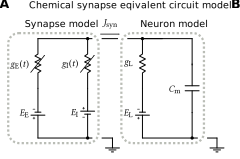
\includegraphics[scale=0.3333]{media/chapters/02_modelling/02_02/synapse_model.pdf}%
	\includegraphics{media/chapters/02_modelling/02_02/synapse_model_traces.pdf}%
	{\phantomsubcaption\label{fig:synapse_model_circuit}}%
	{\phantomsubcaption\label{fig:synapse_model_traces}}%
	\caption[The conductance-based synapse model]{The conductance-based synapse model.
	\textbf{(A)} Circuit diagram of a passive cell membrane with synaptically controlled excitatory and inhibitory conductance-based channels.
	\textbf{(B)} Illustrative voltage, current, and conductance traces. \emph{Top:} Excitatory and inhibitory channel conductances after a pre-synaptic action potential (grey dashed line). \emph{Middle:} Resulting excitatory and inhibitory post-synaptic potentials. \emph{Bottom:} Corresponding excitatory and inhibitory post-synaptic currents.}
	\label{fig:synapse_model}
\end{figure}

\subsubsection{Conductance-based chemical synapse model}
Most gated ion channels can be modelled as a voltage-resistor pair with variable conductance per receptor type \citep{roth2009modeling}.
This is depicted in \Cref{fig:synapse_model} for generic \enquote{excitatory} and \enquote{inhibitory} receptors.
Mathematically, the post-synaptic current $J_\mathrm{syn}(t)$ flowing from the synapse into the neuron is given as
\begin{align}
	J_\mathrm{syn}(t) &=
		  g_\mathrm{E}(t) \bigl(E_\mathrm{E} - v(t)\bigr)
		+ g_\mathrm{I}(t) \bigl(E_\mathrm{I} - v(t)\bigr) \,.
	\label{eqn:conductance_synapse}
\end{align}
Here, $E_\mathrm{E}$ and $E_\mathrm{I}$ are the equilibrium potentials of the gated ion channels.
These potentials are not necessarily equal to ion reversal potentials (\Cref{tbl:nernst}).
For example, NMDA and AMPA channels conduct both $\mathrm{Na^+}$ and $\mathrm{K^+}$, resulting in $E_\mathrm{E} \approx \SI{0}{\milli\volt}$ \citep[Chapter~10]{kandel2012principles}.
%All receptors with the same reversal potential are summarised as single channel in the equivalent circuit.
%Correspondingly, $g_\mathrm{E}$ and $g_\mathrm{I}$ are the sum over the state of multiple post-neurons (similar to \Cref{fig:electrical_circuit_individual_channels}).

\subsubsection{Synaptic dynamics and weights}
The time course of the conductance $g(t)$ depends on the neurotransmitter and receptor type.
Generally speaking, as illustrated in \Cref{fig:synapse_model_traces}, the conductance rises quickly after a spike is received, and decays slowly as the neurotransmitter unbinds from the receptors.
Receptors directly controlled by neurotransmitters acting as ligands (\Cref{fig:synapse}) tend to have relatively short time-constants between $1$ and \SI{100}{\milli\second} \citep{jones2014neurotransmitter}.
Some receptors (e.g., \enquote{metabotropic receptors}) rely on indirect chemical cascades, leading to longer time-constants \citep[Chapter~14]{meriney2019synaptic}; this is not captured well by the models we present here \citep{roth2009modeling}.

\begin{figure}
	\includegraphics{media/chapters/02_modelling/02_02/synapse_filter_examples.pdf}
	{\phantomsubcaption\label{fig:synapse_filter_examples_time_constants}}%
	{\phantomsubcaption\label{fig:synapse_filter_examples_traces}}%
	\caption[Second- and first-order exponential synaptic low-pass filter dynamics]{Illustration of the second- and first-order exponential synaptic low-pass filter dynamics. \textbf{(A)} Impulse response of the second-order dynamics for different $\tau_1$ and $\tau_2$. \emph{Top:} visualisation of the time-constants used below. Swapping $\tau_1$ and $\tau_2$ does not change the dynamics (grey crosses). \emph{Bottom:} Impulse response of the filters (responses normalised to equal area), circles are the peaks. \textbf{(B)} Illustration of post-synaptic conductance traces (\emph{bottom}) according to \Cref{eqn:low_pass_second_order,eqn:low_pass_first_order} for two pre-neurons producing action-potentials (\emph{top}) connected with two different synaptic weights $w_1$, $w_2$.}
\end{figure}

Ligand-gated receptor dynamics are often modelled as a second-order linear dynamical system.
Let $t_{ij}$ denote the time of the $j$th pre-synaptic spike arriving from the $i$th pre-neuron, and let $\tau_1$, $\tau_2$ denote the rise and delay times (\Cref{fig:synapse_filter_examples_time_constants}).
We have \citep{roth2009modeling}:
\begin{align}
	\dot g_1(t) &= -\frac{g_1(t)}{\tau_\mathrm{1}} + g_2(t) \,, &
	\dot g_2(t) &= -\frac{g_2(t)}{\tau_\mathrm{2}} + \sum\nolimits_{i} \alpha w_i \sum\nolimits_{j} \delta(t_{ij} - t) \,,
	\label{eqn:low_pass_second_order}
\end{align}
where $\delta(t)$ is the Dirac-delta, and $\alpha$ is a scaling factor such that the scalar $w_i$ corresponds to the peak value of $g_1(t)$ for a single action potential received from pre-neuron $i$ (\Cref{fig:synapse_filter_examples_traces}).
For $\tau_1 = \tau_2$ this type of synaptic dynamics follow the so-called \emph{alpha function}.

Notably, the scalar $w_i$ is referred to as \emph{synaptic weight} in computational modelling, or as \emph{synaptic strength} in neuroscience.
This scalar summarises various biological processes that determine the average response of the post-neuron to an action-potential received from the $i$th pre-neuron.
For example, synaptic strength can depend on the amount of neurotransmitter released in the pre-synapse, or the ion-channel density in the post-synapse \citep[Chapter~12]{kandel2012principles}.
In this context, the term \emph{synaptic plasticity} refers to a change in synaptic strength over time.
This plays a key role in learning---we discuss this in more detail in Chapter~5.


Typically, the rise-time of $g(t)$ is relatively short.
Correspondingly, the second-order low-pass filter can be approximated by a first-order dynamical system with decay-time $\tau$.
Mathematically, and as depicted the lower portion of \Cref{fig:synapse_filter_examples_traces}, the dynamics are
\begin{align}
	\dot g(t) &= -\frac{g(t)}{\tau} + \sum\nolimits_{i}  w_i \sum\nolimits_{j} \delta(t_{ij} - t) \,.
	\label{eqn:low_pass_first_order}
\end{align}

\subsubsection{Synaptic dynamics as filters}
The above synaptic dynamics (eqs.~\ref{eqn:low_pass_second_order}, \ref{eqn:low_pass_first_order}) are linear time-invariant (\LTI) systems.
%of the form $\dot{\vec g}(t) = \mat A{\vec g(t)} + \mat B u(t)$, where $\mat A \in \mathbb{R}^{n \times n}$ is a state-transition matrix, $\mat B \in \mathbb{R}^{n \times 1}$ is the input matrix, and $u(t)$ is the input in the form of weighted pre-synaptic spike events; the output of the system (i.e., the conductance) is simply the first state-dimension $g_1$.
\LTI systems are fully characterised by their \emph{impulse response} $h(t)$ and can be replaced by a convolution (\enquote{$\ast$}) between $h(t)$ and the weighted input spike-train $u(t)$:
\begin{align}
	g(t)
		&= (h \ast u)(t)
		 = \int_0^\infty h(\tau) u(t - \tau) \,\mathrm{d}\tau
		 = \int_0^\infty h(\tau) \sum\nolimits_{i}  w_i \sum\nolimits_{j} \delta(t_{ij} - \tau) \,\mathrm{d}\tau \,.
	\label{eqn:synapse_impulse}
\end{align}
For the first-order dynamics in \cref{eqn:low_pass_first_order}, the impulse response is $h(t) = \exp(-t/\tau)$ for $t \geq 0$ (and $h(t)= 0$ if $t < 0$); impulse responses of the second-order system are depicted in \Cref{fig:synapse_filter_examples_time_constants}.
Convolutions such as \cref{eqn:synapse_impulse} can alternatively be expressed as multiplication of the frequency contents of the impulse response $h(t)$ and the input spike-train $u(t)$:
\begin{align}
	g(t) &= \mathcal{F}^{-1} \bigl(\mathcal{F}(h) \mathcal{F}(u) \bigr)(t) \,,
\end{align}
where $\mathcal{F}$ is the forward Fourier transformation, and $\mathcal{F}^{-1}$ its inverse.
From this signal-processing perspective, the synaptic dynamics attenuate frequencies in the input spike-train; they act as a \emph{filter}.
The synaptic dynamics discussed so far attenuate low frequencies far less than higher frequencies; they are thus referred to as \emph{low-pass filters}.

% TODO: Talk about filters in general
% TODO: Provide some example synaptic time constants

\newpage

\subsection{Simplified Neuron Models}
\label{sec:simplified_neuron_models}

The models discussed in the previous section describe indiviudal neurons at a relatively low level of abstraction.
This incurs a high computational cost, especially when considering detailed compartemental neurons with Hodgkin-Huxley-like super-threshold dynamics.

Fortunately, important electrophysiological properties of neurons can be captured by less detailed, computationally inexpensive, models \citep[cf.][Chapter~14]{koch1999biophysics}.
For example, the Izhikevich \citep{izhikevich2004which} and Adaptive Exponential \citep{brette2005adaptive} point neuron models require only two state variables, but are capable of reproducing spike patterns observed in nature.
Here, we focus on the even simpler \enquote{leaky integrate-and-fire} (\LIF) model.

\subsubsection{The leaky integrate-and-fire model}

\begin{figure}[t]
	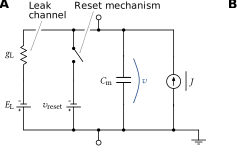
\includegraphics[scale=0.3333]{media/chapters/02_modelling/02_02/lif_circuit.pdf}%
	\kern-0.25cm\includegraphics{media/chapters/02_modelling/02_02/lif_traces.pdf}
	\caption[Equivalent circuit diagram and membrane potential trace of a LIF neuron]{Equivalent circuit diagram and membrane potential trace of a \LIF neuron. \textbf{(A)} The \LIF model consists of a capacitative membrane with a \enquote{leak} channel. A reset mechanism clamps \vMem to the reset potential \vReset. \textbf{(B)} Membrane potential trace (\emph{top}) for rectangle pulse current inputs (\emph{middle}).  Vertical dashed lines are spike events. The bottom graph depicts the remaining refractory period.}
	\label{fig:lif}
\end{figure}

%\footnote{Extensions to the LIF model include the quadratic and exponential integrate-and-fire models (QIF and EIF, respectively). Hence, LIF is sometimes read as \enquote{linear integrate-and-fire}. Furthermore, there is the IF model, that does not include a leak channel, sometimes also called nLIF (non-leaking).}
A variant of the \LIF model---lacking refractoriness---dates back to \citet{lapicque1907recherches}.
Just like the Hodgkin-Huxley model (\Cref{sec:neural_dynamics}), the \LIF neuron is based on a capacitive membrane with a leak channel.
The input current is integrated by the capacitor, which, at the same time, is discharged through the leak channel:
\begin{align}
	\CMem \dot{\vMem}(t) =
		\gL \bigl(\EL - \vMem(t)\bigr) + J(t) \,,
	\label{eqn:lif}
\end{align}
where \gL is the leak conductance, \EL is the leak reversal potential, and $J(t)$ is a (synaptic) current injected into the membrane.
Unlike the Hodgkin-Huxley model, the dynamics of the system do not model spike production; \enquote{firing} is handled outside the dynamical system. 
Once $\vMem(t)$ reaches a threshold $\vTh$, a spike event is recorded and \vMem is held at the \emph{reset potential} \vReset for the duration of the refractory period \tauRef.
This is depicted in \Cref{fig:lif}.

\subsubsection{Response curve}

\begin{figure}
	\centering
	\includegraphics{media/chapters/02_modelling/02_02/neuron_voltage_traces.pdf}
	\caption[Voltage traces for the LIF and Hodgkin-Huxley neuron model]{Voltage traces (\emph{top}) for the \LIF and a Hodgkin-Huxley-type neuron dynamics described by \citet{traub1991neuronal} given a current ramp input~(\emph{bottom}). Dashed vertical lines correspond to spike events. Dotted line is the resting potential at $\EL=\SI{-65}{\milli\volt}$. Both neurons have a membrane capacitance of $C_\mathrm{m} = \SI{200}{\pico\farad}$ and a leak conductance of $g_\mathrm{L} = \SI{10}{\nano\siemens}$. \textbf{(A)} The \LIF neuron model does not account for spike production; the voltage is simply reset to $v_\mathrm{reset} = \SI{-85}{\milli\volt}$ for $\tauRef = \SI{2}{\milli\second}$ once the membrane potential passes the threshold at $v_\mathrm{th} = -\SI{55}{\milli\volt}$. \textbf{(B)} Same experiment for a Hodgkin-Huxley neuron. Notably, the super-threshold dynamics of the Hodgkin-Huxley model action potentials and the first spike appears significantly earlier compared to the \LIF neuron.}
	\label{fig:neuron_voltage_traces}
\end{figure}

\begin{figure}
	\centering
	\includegraphics{media/chapters/02_modelling/02_02/neuron_response_curves.pdf}%
	{\phantomsubcaption\label{fig:neuron_response_curves_lif}}%
	{\phantomsubcaption\label{fig:neuron_response_curves_hh}}%
	\caption[Response curves for the LIF and Hodgkin-Huxley-type neuron model]{Response curves (also called IF-curves) $G[J]$ for the \LIF and Hodgkin-Huxley-type neuron model from \Cref{fig:neuron_voltage_traces}. Data extracted from the inter-spike-intervals of a current ramp experiment (sweep from \SIrange{0}{2}{\nano\ampere} over ten seconds at a \SI{10}{\micro\second} resolution). Although the \LIF and Hodgkin-Huxley models have drastically different dynamics, their response curves are qualitatively similar.}
	\label{fig:neuron_response_curves}
\end{figure}

\begin{figure}
	\centering
	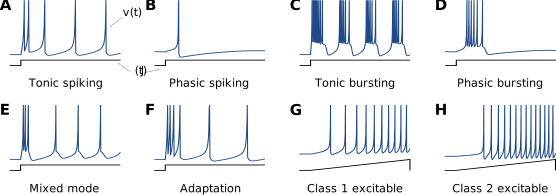
\includegraphics{media/chapters/02_modelling/02_02/izhikevich_whichmod_figure1.pdf}%
	{\phantomsubcaption\label{fig:izhikevich_whichmod_figure1a}}%
	{\phantomsubcaption\label{fig:izhikevich_whichmod_figure1b}}%
	{\phantomsubcaption\label{fig:izhikevich_whichmod_figure1c}}%
	{\phantomsubcaption\label{fig:izhikevich_whichmod_figure1d}}%
	{\phantomsubcaption\label{fig:izhikevich_whichmod_figure1e}}%
	{\phantomsubcaption\label{fig:izhikevich_whichmod_figure1f}}%
	{\phantomsubcaption\label{fig:izhikevich_whichmod_figure1g}}%
	{\phantomsubcaption\label{fig:izhikevich_whichmod_figure1h}}%
	\caption[Diversity of neural dynamics for constant or ramp input currents]{Diversity of neural dynamics for constant or ramp input currents. Each plot depicts membrane-potential traces $v(t)$ (\emph{top}) of the Izhikevich neuron model (with different parameters) for an input current $J(t)$ (\emph{bottom}). \LIF neurons are only capable of behaviours \emph{A} and \emph{G}. Partially reproduced (dynamics for input pulses were skipped) with minor modifications from \citet{izhikevich2004which}. Electronic version of the figure and reproduction permissions freely available at \url{http://www.izhikevich.org}.}
	\label{fig:izhikevich_whichmod_figure1}
\end{figure}

\Cref{fig:neuron_voltage_traces} depicts a comparison between the Hodgkin-Huxley-type and \LIF dynamics.
The reset and threshold potential of the \LIF neuron model have been tuned to match the sub-threshold membrane potentials observed in the Hodgkin-Huxley neuron.
In both cases---apart from the obviously missing super-threshold dynamics---the inter-spike-interval decreases the larger $J$, leading to a higher spike rate.
This suggests a characterisation of neurons in terms of their \emph{response curve} $G[J]$ (\Cref{fig:neuron_response_curves})
\begin{align}
	G[J] &= \lim_{T \to \infty} \frac{n_\mathrm{spikes}(J, T)}{T} \,, & \text{where } n_\mathrm{spikes}(J, T) &= \text{\#spikes for input $J$ over a period $T$} \,.
	\label{eqn:response_curve}
\end{align}
Of course, this only makes sense if we assume that the neuron has a non-zero steady-state activity for a constant superthreshold input current.
This is not necessarily true; neurons can exhibit complex behaviours that violate this assumption \citep{izhikevich2004which}.
For example, \emph{phasic} neurons only produce a limited number of spikes in response to an input step (Figure~\ref{fig:izhikevich_whichmod_figure1}B, D, E), while other neurons adapt to constant input currents over time, resulting in a reduction in frequency (Figure~\ref{fig:izhikevich_whichmod_figure1}F).
Still, neurons often behave \emph{tonically} (Figure~\ref{fig:izhikevich_whichmod_figure1}A, C, G, H), and can be reasonably well characterised in terms of a response curve.

Response curves and time-less \enquote{rate neurons} form the basis for artificial neural networks commonly used in machine learning. We discuss this in more detail later in this thesis.
Furthermore, we revisit temporal properties of the response curve when we discuss temporal tuning curves. % LEAVE SPACE HERE
% TODO add section references

\subsubsection{LIF response curve}
For most neuron models, it is impossible to derive a closed-form expression for the average spike rate $G[J]$ given a constant current $J$; there typically is no closed-form solution for $G[J]$. 
%\footnote{Very few differential equations posses closed-form solutions. Even slightly more complex models (e.g.,~first-order current-based synapses instead of constant $J$) require the analytic Lambert $\mathcal{W}$ function in the solution.}
Instead, we have to rely on the method suggested by \cref{eqn:response_curve}.
That is, we simulate the neural dynamics for a sufficiently long time-period and count the number of spikes $n_\mathrm{spikes}$.

The \LIF neuron is a notable exception to this, as its subthreshold dynamics form a simple first-order linear dynamical system.
Using basic techniques for solving differential equations, the membrane potential \vMem at time $t$ for a constant input current $J$ is given as
\begin{align}
	v(t) &= \left(1 - e^{-\frac{t}{\tauMem}} \right) \left( \EL + \frac{J}{\gL} \right) + e^{-\frac{t}{\tauMem}} v(0) \,, &&\Rightarrow & \lim_{t \to \infty} v(t) &= \EL + \frac{J}{\gL} \,.
\end{align}
To compute the average spike rate, we need to know how long it takes to reach the threshold potential after a spike has been issued.
To this end, we simply solve $v(t_\mathrm{spike}) = \vTh$ with $v(0) = \vReset$ for $t_\mathrm{spike}$.
Keeping in mind that the neuron is held at the reset potential for $\tauRef$ seconds after every spike, and defining the threshold current $J_\mathrm{th} = (\vTh - \EL) \gL$, we have
\begin{align}
	\begin{aligned}
	G[J] &= \begin{cases}
		0 & \text{if } J \leq J_\mathrm{th} \,, \\
		\frac{1}{\tauRef + t_\mathrm{spike}} & \text{if } J > J_\mathrm{th} \,,
	\end{cases} & \quad
	\text{where }
%	J_\mathrm{th} &=
%		(\vTh - \EL) \gL \,, \\
	t_\mathrm{spike} &=
		-\tauMem \log\left(1 - \frac{(\vTh - \vReset) \gL}{(\EL - \vReset) \gL + J} \right) \,.
	\end{aligned}
	\label{eqn:lif_response_curve}
\end{align}
As depicted in \Cref{fig:neuron_response_curves_lif}, the predicted rate perfectly matches the empirical measurement.
Notably, the \LIF response curve is qualitatively similar to that of the Hodgkin-Huxley neuron (\Cref{fig:neuron_response_curves_hh})---surprisingly so, as the dynamical systems differ wildly between the two models.
This makes \LIF neurons a reasonable choice for simulating large-scale neurobiological systems at small computational costs (\cite{meunier2002playing}).

\subsubsection{Simplified LIF neuron}
A qualitatively equivalent form of the \LIF neuron is given by normalising the voltages such that $\EL = 0$ and $\vTh = 1$, and furthermore setting $J_\mathrm{th} = 1$:
\begin{align}
	\dot v(t) &= -\frac{1}{\tauMem} v(t) + J(t) \,, &
	G[J] &= \begin{cases}
		0 & \text{if } J \leq 1 \,, \\
		\frac{1}{\tauRef - \tauMem \log\left(1 - \frac{1 - \vReset}{J-\vReset}\right)} & \text{if } J > 1 \,.
	\end{cases}
	\label{eqn:lif_simplified}
\end{align}
The primary advantage of this form is the reduction in mathematical operations compared to \cref{eqn:lif}.
This simplification (among other optimisations) is exploited by the neural network simulator \enquote{Nengo} to support large-scale spiking neural network simulations \citep{bekolay2014nengo}.
The downside is a reduced interpretability of the now unit-less $v(t)$ and $J(t)$.

\subsubsection{Current-based synapse models}
Another possible simplification---both in terms of computation and mathematical analysis---concerns the synapse model.
In conductance-based synapses (\Cref{sec:synaptic_transmission}) the current $J_\mathrm{syn}(t)$ explicitly depends on the membrane potential $\vMem(t)$.
Going back to \Cref{fig:synapse_model_traces}, one may notice that the post-synaptic currents can be approximated as a scaled version of the conductance \citep[cf.][]{roth2009modeling}.

This suggests modelling the post-synaptic current $J_\mathrm{syn}$ as a linear superposition of filtered spike events.
Let the synaptic weight $w_i$ denote the peak post-synaptic current.
Then, the first-order \emph{current-based} synapse model is given as (analogously for higher-order filters)
\begin{align}
	\dot J_\mathrm{syn}(t) &= -\frac{J_\mathrm{syn}(t)}{\tau} + \sum\nolimits_{i}  w_i \sum\nolimits_{j} \delta(t_{ij} - t) \,.
	\label{eqn:low_pass_first_order_current}
\end{align}
We compare conductance- and current-based synapse models in more detail in the next chapter.

\pagebreak

\subsection{Spiking Neural Networks}
\label{sec:neural_networks}

\begin{figure}
	\centering
	
\includegraphics{media/chapters/02_modelling/02_02/neural_networks.pdf}%
	{\phantomsubcaption\label{fig:neural_networks_a}}%
	{\phantomsubcaption\label{fig:neural_networks_b}}%
	{\phantomsubcaption\label{fig:neural_networks_c}}%
	\caption[Illustration of different neural network types]{Illustration of different neural network types. Blue circles depict individual neurons. \textbf{(A)} Feed-forward neural networks can be represented as acyclic graphs. \textbf{(B)} If the network connectivity contains cycles (e.g., the 5-2-4-5 cycle), the network is called \emph{recurrent}. Cycles can also be self-recurrences (e.g., neuron 6). \textbf{(C)} Artifical neurons (\emph{left}) process time-discrete samples. Spiking neurons (\emph{right}) are time-continous; they receive a weighted input spike train, filter it, and produce an output spike train.}
\end{figure}

% How to build neural networks
% Define feed-forward and recurrent neural networks
% But how to select the weights?
% Solution that artificial neural networks do
% But is this what biology does?
% Rate vs temporal coding debate -> Aaron

We are now well-equipped to construct and simulate spiking neural networks (\SNNpl).
In theory, we just take $n$ spiking neurons and connect them up according to synaptic weights $w_{ij}$. As mentioned before, these weights determine the connection strength between a pre-neuron $j$ and post-neuron $i$. Inputs are additive over multiple pre-neurons (eqs.~\ref{eqn:low_pass_first_order}, \ref{eqn:low_pass_first_order_current}).%
\footnote{This notion of synaptic weights $w_{ij}$ assumes that each neuron possesses a single synaptic input channel.
Hence, there is only a single synaptic weight matrix.
For neurons with multiple synaptic input channels we can simply use an individual weight matrix for each input channel. We discuss this in the next chapter.}

Mathematically, the \emph{weight matrix} $\mat W \in \mathbb{R}^{n \times n}$ is the adjacency matrix of a directed connectivity graph.%
\footnote{For convenience and computational efficiency, neurons are typically grouped into \enquote{layers}, \enquote{populations}, or \enquote{ensembles} (all terms are used synonymously).
Not all layers have connections among each other. Hence, $\mat W$ typically is a block-matrix that can be split into multiple sub-matrices.}
Networks with acyclic connectivity are called \emph{feed-forward} (\Cref{fig:neural_networks_a}); networks with cyclic connectivity are \emph{recurrent} (\Cref{fig:neural_networks_b}).
Feed-forward \SNNpl have finite memory.
Assuming plausible synaptic filters, their impulse response decays exponentially.
In contrast, and as we discuss later, recurrent networks can posses more interesting dynamics.

To actually simulate an \SNN, we feed an external input (e.g., a set of currents or spike-trains) into the network and numerically integrate the coupled differential equations.
There are numerous general-purpose simulator software packages that do this efficiently, e.g., NEST \citep{gewaltig2007nest}, Brian \citep{stimberg2019brian}, GeNN \citep{yavuz2016genn}, or Nengo \citep{bekolay2014nengo}.

The most important question---and one that we pursue for the remainder of this thesis---is how to ultimately select $\mat W$.
For the artificial neural networks ({\ANN}s) used in machine learning (\Cref{fig:neural_networks_c}), the astoundingly successful answer is to use stochastic gradient descent on a loss function $E$, i.e., $\dot{\mat W} = -\eta \nabla_{\mat W} E(\vec a_k, \vec {\hat a_k})$, where $\eta$ is a learning rate, $\vec a_k$ is the desired output activity for an input sample $\vec x_k$, and $\vec{\hat a_k}$ is the actual output \citep{lecun2015deep}.
For example, one common choice for the loss function is $E(\vec a_k, \vec {\hat a_k}) = \|\vec a_k - \vec{\hat a}_k\|^2$.

Similar gradient-descent global optimisation methods can be applied in the context of \SNNpl as well.
\Citet{hunsberger2018spiking} characterises the \LIF response curve $G[J]$ in a network context and then trains an \ANN that uses $G[J]$ as a nonlinearity.
The resulting $\mat W$ can then be used in a spiking context.
\Citet{goltz2020fast} optimise synaptic weights such that desired spike-timings are generated by a black-box spiking neural network simulator.

%Computational neuroscientists often distinguish between rate and temporal spike-codes, though the definitions of these concepts are quite vague.
%For example, \citet[Chapter~1]{gerstner2002spiking} list three different definitions of the term \enquote{rate code}, while \citet{abbott2001theoretical} list four definitions.
%Rates are estimated by either binning and counting, causal and acausal filtering, or (orthogonally) taking averages over entire populations into account.

%A similar zoo of definitions is to be had for temporal codes. For example, as pointed out by \citet[Chapter~14]{koch1999biophysics}, researchers often interpret temporal codes as correlations between spike times carrying information (i.e., spikes from different pre-neurons arriving earlier or later relative to each other).
%Another popular temporal code is \enquote{time-to-first-spike}, i.e., the notion that neurons rely on the time between some synchronisation event and the first received spike event \citep{vanrullen2005spike}.

Notably, such global optimisation methods can be useful when modelling neurobiological systems.
For example, there are striking similarities between the neural tuning observed in visual cortex and the learned tuning of neurons in hierarchical image classification networks \citep{yamins2016using}.
However, this is, to some degree, accidental, and not explicitly imposed.
As we discussed at the beginning of this chapter, it is desirable build models that reliably adhere to certain constraints---such as the aforementioned tuning properties.

\subsection{Neural Tuning and Population Codes}
\label{sec:neural_tuning}

\begin{figure}
	\centering
	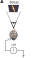
\includegraphics{media/chapters/02_modelling/02_02/visual_cortex_tuning_setup.pdf}%
	\includegraphics{media/chapters/02_modelling/02_02/visual_cortex_tuning.pdf}
	\caption[Neural tuning in the visual cortex]{Neural tuning in the visual cortex.
	\textbf{(A)} Illustration of the original experiment by \citet{hubel1959receptive}. Bright rectangles are briefly presented on a dark screen to an animal while recording from a neuron in its visual cortex. \textbf{(B)} Recorded spike trains for different stimulus orientations. Horizontal lines are the stimulus presentation interval. Adapted from \citet[Figure~3]{hubel1959receptive}. \textbf{(C)} The mapping between stimulus $\vec x$ and activity $a$ forms a \emph{tuning curve}. This neuron is tuned to vertical bars.}
	\label{fig:visual_cortex_tuning}
\end{figure}

%Given that we can simulate large biological systems at different levels of abstraction, the primary challenge is to construct networks that actually give rise to the behaviours observed in nature.
%Unfortunately, in many cases, too much about the brain is still unknown to successfully build such models.
%This is particularly true for brain regions involved in higher level cognition, and that, in terms of connectivity, are farther away from the periphery.
%Fortunately, brain regions \emph{closer} to the periphery are, relatively speaking, quite well understood.
%\footnote{Neuroscience textbooks such as \citet{kandel2012principles} discuss the neural circuitry of brain regions involved in sensory and motor processing in great detail, while chapters concerning higher-level cognitive tasks mostly report behavioural observations and coarse measurements such as fMRI scans.}
There are two important concepts that shed some light onto the organisation of brain networks---at least those brain networks involved in sensory processing: \emph{tuning curves} and \emph{receptive fields}.
In turn, these ideas motivate \emph{population codes}, which we heavily rely on in the context of our modelling tool, the Neural Engineering Framework---we discuss this in the next section.

\subsubsection{Tuning curves}
%Early studies on these concepts were conducted by \citeauthor{hubel1959receptive}.
In a famous \citeyear{hubel1959receptive} experiment (cf.~\Cref{fig:visual_cortex_tuning}), Hubel and Wiesel present a visual stimulus in the form of a bright rectangle at different orientations $\varphi$ to an experimental animal.
At the same time, the activity of a neuron in the animal's visual cortex is recorded.
This characterizes how the stimulus propagates through the brain up to the recording site.
%We characterize neurons in terms of their own physiological properties \emph{and} in terms of the preceding network connectivity.

In the recording depicted in \Cref{fig:visual_cortex_tuning}, we find that the neuron is most sensitive to---or, \emph{tuned} to---a certain orientation $\varphi$.
We could say that in this specific case, vertical bars are the \emph{preferred stimulus} of the neuron.
Generally, such a mapping from a stimulus property $\varphi$ onto the average neural activity $a(\varphi)$ is called a \emph{tuning curve} \citep[e.g.,][p.~1112]{vandenbos2015apa}.

\subsubsection{Receptive fields}

\begin{figure}
	\centering
	\includegraphics{media/chapters/02_modelling/02_02/gabor_filters.pdf}
	\caption[Examples of randomly generated of Gabor filters]{Examples of randomly generated Gabor filters.
	Each filter is a two-dimensional function $e(\xi_1, \xi_2)$, where $(\xi_1, \xi_2)$ is a spatial location.
	Negative  values (red) indicate that neural activity is reduced if a stimulus is present at that location, positive values (blue) indicate an increase in activity.}
	\label{fig:gabor}
\end{figure}
The concept of \emph{receptive fields} is closely related to tuning curves.
This is best illustrated in the context of stimuli that can be described as an intensity over a two-dimensional surface---such as vision or touch.
Generally, the receptive field of a neuron is the collection of points $(\xi_1, \xi_2)$ at which the presence of a stimulus---a point of light or mechanical pressure---triggers a neural response.
However, as evidenced by \citet{hubel1962receptive}, neural receptive fields are not only characterised in terms of the locations where a stimulus \emph{increases} the average neural activity, but also where the presence of a stimulus \emph{decreases} activity.

Mathematically, we can describe this in terms of a function $e(\xi_1, \xi_2)$ that assigns a weight to each stimulus location $(\xi_1, \xi_2)$.
This function $e$ is the receptive field.
\emph{Gabor filters} are a class of mathematical functions that fit observed receptive fields in the visual cortex well \citep{marcelja1980mathematical,field1986structure}.%
\footnote{Gabor filters are sinusoidals scaled by a radial Gaussian envelope. Such functions are maximally localised in time and space, as pointed out in the context of Gabor's Fourier uncertainty principle \citep{gabor1946theory}.}
Examples are depicted in \Cref{fig:gabor}.

Borrowing some notation from the next section, the activity of the neuron $a(x)$ can be modelled as the product between the receptive field $e$ and the stimulus $x$ integrated over space (where $x(\xi_1, \xi_2)$ is a function describing the stimulus intensity at a certain location)
\begin{align}
	a(x) &= G\left[ \alpha \iint e(\xi_1, \xi_2) x(\xi_1, \xi_2) \,\mathrm{d}\xi_1\mathrm{d}\xi_2 + \beta \right]
		= G \bigl[ \alpha \langle e, x \rangle + \beta \bigr] \,.
	\label{eqn:tuning_curve_from_receptive_field}
\end{align}
Here, $\langle e, x \rangle$ is the inner product between the receptive field and the stimulus (see \Cref{app:functional_analysis} for an introduction to functional analysis and the corresponding definitions).
Furthermore, $G$ is a rate approximation of the neuron model (see previous subsection), and, $\alpha > 0$ and $\beta$ translate the inner product into a neural input current.

Importantly, if the stimulus and receptive field are normalised, then $\langle e, x \rangle$ is the cosine similarity between the two functions.
Correspondingly, according to the above model, the neural response is maximised if $e = x$.
In other words, the receptive field \emph{is} the \enquote{true} preferred stimulus of a neuron.
This is consistent with modern definitions of the term \enquote{receptive field} in the neuroscience literature \citep[cf.][]{troy2009retinal}.

\begin{figure}
	\centering
	\includegraphics{media/chapters/02_modelling/02_02/visual_cortex_receptive_field_example.pdf}
	\caption[Model of the Hubel and Wiesel experiment]{Model of the original Hubel and Wiesel experiment (cf.~\Cref{fig:visual_cortex_tuning}). \textbf{(A)} The receptive field $e(\xi_1, \xi_2)$ describes whether a stimulus location $(\xi_1, \xi_2)$ acts excitatory (blue), or inhibitory (red). \textbf{(B)} The stimulus is a light rectangle at different orientations $\varphi$; this can be described as a function $x$ mapping locations onto light intensity. \textbf{(C)} Tuning curve obtained according to the model in \cref{eqn:tuning_curve_from_receptive_field}.}
	\label{fig:visual_cortex_receptive_field_example}
\end{figure}

\Cref{fig:visual_cortex_receptive_field_example} illustrates the relationship between the receptive field of a neuron and one of its tuning curves.
Choosing a vertically oriented Gabor filter as a receptive field, we can model the orientation tuning from the original Hubel and Wiesel experiment.
Thus, in a nutshell, a tuning curve is a characterisation of the neuron in terms of a specific stimulus property (e.g., the orientation of a bar of light), whereas the receptive field models its tuning properties in general (e.g., the predicted activity for any visual stimulus).

\subsubsection{Population codes}
Although tuning curves and receptive fields are inherently reconstructed from a network context, they still only characterise individual neurons.
To better understand biological neural networks, we need to consider the tuning properties of groups of neurons.

Doing this, we find that neighbouring neurons often have similar tuning properties---they are tuned to the same sensory modality, and possess similar receptive fields \citep{berkowitz2009population}.
Again, this has been explored well in context of orientation tuning in the visual cortex \citep[Chapter~25]{kandel2012principles}.
For example, neurons in visual cortex are organised in \enquote{cortical columns}.
Each column consists of several layers of neurons.
Within a single layer of the same column, neurons possess the similar preferred orientations.
Between columns, preferred orientations differ significantly.

This, as well as several other observations \citep{yuste2015neuron}, suggest that brain networks use \emph{population codes}.
The idea is that a single underlying quantity---such as the orientation of a visual stimulus---is represented by a group of neurons in a distributed manner.
The opposite would be \enquote{single-neuron coding}, where the activity of individual, localised neurons maps onto some quantity, or, in higher-level cognition, onto specific concepts \citep{berkowitz2009population}.

\begin{figure}
	\centering
	\includegraphics{media/chapters/02_modelling/02_02/population_code.pdf}
	\caption[Probabilistic decoding of scalar quantities using population codes]{Probabilistic decoding of scalar quantities using population codes.
	\textbf{(A)} \emph{Left:} The activity $a$ of a single neuron represents a scalar value $x \in [-1, 1]$.
	The current $J$ fed into each neuron is subject to Gaussian noise with standard deviation $\sigma = \SI{1}{\nano\ampere}$.
	Solid line corresponds to the median activity for the given represented value; shaded area corresponds to a contour line of the underlying probability density.
	\emph{Right:} Trying to decode the represented value $x$ from the activity results in significant uncertainties; negative values cannot be disambiguated. Dotted line is the optimum; solid line the median of a maximum-likelihood estimate, shaded area a contour line of the underlying probability density.
	Error $E$ is the decoding \RMSE.
	\textbf{(B, C, D)} The larger the number of neurons, the smaller the uncertainties.}
	\label{fig:population_code}
\end{figure}

Population codes are intriguing as a model for representation in biological networks.
They allow precise inferences from imprecise or ambiguous observations. This is illustrated in \Cref{fig:population_code}.
For example, we can imagine that a single neuron represents a scalar value $x \in [-1, 1]$ as expressed by its tuning curve $a(x)$.
Unfortunately, the firing rate $a$ cannot be measured without error.
That is, neurons produce spontaneous activity that, as far as we can tell, is not related to a stimulus.
This is part due to noise inherent to neurobiological processes \citep[cf.][Section~2.2.1]{eliasmith2003neural}, and in part due to the Fourier uncertainty principle.%
\footnote{We can either estimate the frequency (i.e., rate) of a signal with a high precision at a low temporal resolution, or estimate the frequency with a low precision at a high temporal resolution \citep{gabor1946theory}.}
Hence, when trying to \emph{decode} the represented value $x$ from the neural activity, there is a large degree of uncertainty.
Adding neurons that are tuned to the same quantity $x$, but with different tuning curves to the population drastically reduces this uncertainty from a information-theoretic perspective \citep{ma2009population}.


\clearpage
\setcounter{section}{2}
% !TeX spellcheck = en_GB

\section{The Neural Engineering Framework}
\label{sec:nef}

\begin{figure}[p]
	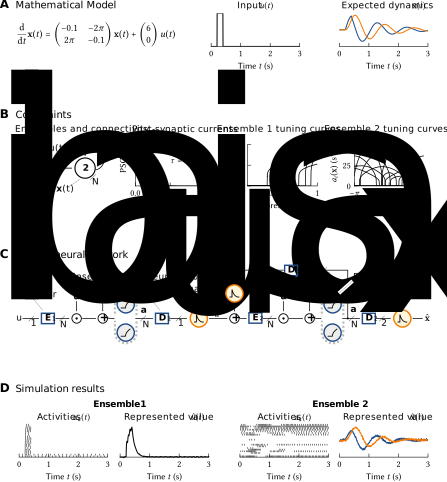
\includegraphics{media/chapters/02_modelling/02_03/nef_overview.pdf}
	\caption[Overview of the Neural Engineering Framework]{Overview of the Neural Engineering Framework (\NEF).
	\textbf{(A,~B)} Researchers provide a mathematical model or sampled data (sampled data shown here are random and only for illustration purposes), as well as a set of constraints.
	In this example, constraints are the overall connectivity, tuning properties and filter properties of post-synaptic currents. $\angle \vec x$ denotes the angle of $\vec x = (x_1, x_2)$, i.e., $\angle \vec x = \mathrm{arctan2}(x_2, x_1)$. \textbf{(C)} The \NEF can be used to systematically construct a spiking neural network from the given data. This network optimally implements the mathematical model under the given constraints.
	\textbf{(D)} Simulating the network gives insights into how well the mathematical description can be implemented on a neural substrate.
	Spike raster plots with neural activity depict output spikes (short vertical lines) for each neuron (corresponding to rows) over time.}
	\label{fig:nef_overview}
\end{figure}

As we mentioned at the beginning of this chapter, the Neural Engineering Framework (\NEF; \cite{eliasmith2003neural}) is a modelling framework for neurobiological systems.
The \NEF combines techniques from engineering and mathematics---particularly control and dynamical systems theory---with the neurobiological concepts discussed before.
The goal is to allow researchers to map high-level descriptions of cognitive phenomena onto low-level spiking neural networks.
As such, the \NEF provides a synthesis of bottom-up and top-down modelling, and is an attempt at a theory of neuroscience that spans multiple levels of analysis.

To use the \NEF, researchers systematically apply three \enquote{principles} that encapsulate key assumptions about neurobiological systems.
These principles exploit neural nonlinearities and synaptic filters to describe how vectorial quantities can be represented, transformed, and made to follow certain dynamics in a spiking neural fabric.
The resulting neural networks adhere to mechanistic constraints, such as neural connectivity, maximum firing rates, tuning properties, and synaptic time-constants.
This is illustrated schematically in \Cref{fig:nef_overview}.
A software tool that automates the process of translating mathematical models into spiking neural networks using the \NEF principles is part of the Nengo spiking neural network simulator package \citep{bekolay2014nengo}.\footnote{See \url{https://www.nengo.ai/} for more information on Nengo. Nengo is free for non-commercial use.}


%\begin{enumerate}[1.]
%	\item \emph{Representation.}
%	The momentary activity $\vec a \in \mathbb{R}^{\Npop}$ of an ensemble of \Npop neurons represents a vectorial quantity $\vec x \in \mathbb{R}^d$. The encoding process mapping $\vec x$ onto activities $\vec a$ is nonlinear,
%	the decoding process is linear.
%	That is, there exists a matrix $\Dec \in \mathbb{R}^{d \times \Npop}$ such that $\vec x \approx \vec \Dec \vec a(\vec x)$.
%	\item \emph{Transformation.}
%	Synaptic connections between neural ensembles approximate nonlinear transformations $f(\vec x)$ applied to the represented values, where $f : \mathbb{R}^d \longrightarrow \mathbb{R}^{d'}$ and $d$ and $d'$ are the dimensionalities of the quantities represented in the individual ensembles.
%	\item \emph{Dynamics.}
%	Represented values are state variables $\vec x(t)$ in a dynamical system. Recurrent connections approximate arbitrary dynamical systems of the form $\dot{\vec x} = f(\vec x(t), \vec u(t), t)$.
%	Here, $\vec x(t)$ is the represented value, $\vec u(t)$ is some external input, and $t$ is the current time.
%\end{enumerate}

In this section, we first discuss applications of the \NEF from the perspective of the cognitive sciences (model validation and hypothesis generation), as well as engineering and computer science (a programming model for neuromorphics).
We continue with a detailed description of the theory underpinning the \NEF, and conclude with a list of limitations that we address in the next chapters.

\subsection{Model Validation and Hypothesis Generation}
\label{sec:nef_purpose}

As we alluded to in the introduction of this chapter, models built using the \NEF bridge multiple levels of analysis.
That is, they implement high-level behaviour (given as a mathematical description) using low-level mechanisms (spiking neurons and synapses).
This facilitates model validation and hypothesis generation.

\subsubsection{Model validation}
The concept of model validation generally refers to comparing a model to empirical measurements \citep{adams2012assessing}.
In the case of \NEF models, we can, of course, compare the high-level behaviour of the biological system to that of the constrained network model.
The smaller the deviations, the \enquote{better} the original mathematical model.%
\footnote{Of course, naively evaluating models in this manner does not account for overfitting. The model could inadvertently be tuned to reproduce the behaviour of interest, but not be able to generalise to different scenarios. In contrast to other machine learning approaches, overfitting in this sense is typically less of a problem with \NEF models.
This is due to the transparency of the training process, only few (typically hand-selected) parameters, and biological constraints, all of which can be seen as regularisation.}
While such comparisons would also be possible with the high-level model alone, biological constraints can drastically influence the high-level behaviour of the model.
The \NEF is thus a good litmus test for the suitability of a mathematical model to be realised on a neural substrate.
This is because the \NEF \emph{optimally} implements a set of mathematical equations as an idealised spiking neural network.
If the model cannot be realised on a spiking neural substrate despite these idealised conditions, it is unlikely that it describes a biological process well.

\NEF models can also be compared in terms of detailed neurophysiological data, and not just high-level behaviour.
Because \NEF models are based on a biologically plausible neural substrate, researchers can measure neurophysiological quantities, such as spike trains, local field potentials, or blood oxy\-gen\-ation \citep[Chapters 5.8~\&~9.4]{eliasmith2013how}.
Examples of this can be found in \citet{stewart2012learning,bekolay2014spiking,duggins2017effects,voelker2018improving,gosmann2021cue}.

\subsubsection{Hypothesis generation}
There are two ways in which the \NEF aids \emph{hypothesis generation}.
First, and closely related to model validation, deviations between the constrained simulation and the original mathematical model may indicate that the high-level description cannot be realised by the biological system.
Hence, the \NEF can be used to reject unsuitable hypotheses and to guide theories towards higher degrees of biological plausibility.
Examples of cognitive theories developed in conjunction with the \NEF include the Semantic Pointer Architecture (SPA; \cite{eliasmith2013how}) and SPAUN (the \enquote{Semantic Pointer Architecture Unified Network}), a functional brain model capable of a variety of cognitive tasks \citep{eliasmith2012largescale}.

Second, \NEF models can be used to predict the behaviour of a system in experimental paradigms for which no empirical data exists (yet).
This prediction then forms a hypothesis that can be compared to future empirical data.
Furthermore, the \NEF also enables the systematic variation of observed biological parameters (e.g., time-constants or connectivity), which is often not easily possible in real biological systems.
Assessing the system performance in such artificial situations may yield hypotheses as for why evolution favoured certain parameter combinations.
We give an example of this in \Cref{chp:cerebellum}.

\subsection{Applications to Neuromorphic Computing}
\label{sec:neuromorphic}

The scientific applications discussed above were the primary motivation for the development of the \NEF.
However, coincidentally, the same methods are useful as a programming model for neuromorphic computers \citep{boahen2017neuromorph,voelker2021programming}.

\subsubsection{Neuromorphic computers}
Coined by \citet{mead1990neuromorphic}, this term refers to computer systems that---to some degree---mimic information processing in the brain.
This typically implies numerous simple computational units, \emph{neurons}, connected via a flexible interconnect \citep{furber2016largescale}.
Beyond these basic characteristics there is no consensus as for what exactly constitutes a \enquote{neuromorphic computer}.
However, most neuromorphic hardware systems execute computations asynchronously and possess provisions for sparse event-based signalling.
Akin to biology, individual computational units independently generate binary events.
In contrast to artificial neural networks, computation is inherently temporal; communication occurs sporadically and does not carry continuous values.
Hence, the underlying communication infrastructure solely carries temporally sparse spike events, minimising the amount of transferred data.

Current neuromorphic computers can be roughly split into two categories, depending on the specific realisation of the computing elements.
Computation either takes place in analogue model circuits, similar to the \LIF circuit (\Cref{fig:lif}), or digital processors with varying degrees of programmability.
Examples of systems in the former \enquote{mixed-signal} category include Braindrop \citep{neckar2019braindrop} and BrainScaleS \citep{schemmel2010waferscale}.
Systems that fall into the latter \enquote{purely digital} category are SpiNNaker \citep{furber2013overview} and Loihi \citep{davies2018loihi}. See \citet{furber2016largescale} for a more comprehensive list.

\subsubsection{Applications of neuromorphic computing}
The primary motivation behind neuromorphic hardware is to construct computing hardware that approaches the energy efficiency of biological brains \citep{mead1990neuromorphic,boahen2017neuromorph}.
Compared to conventional computer architectures, these energy savings are mostly due to the asynchronous nature of the computational units, as well as the reduction in communication bandwidth due to event-based signalling \citep{painkras2013spinnaker}.
Furthermore, mixed-signal neuromorphic computers with analogue model circuits benefit from each computational unit operating close to the theoretically required minimum energy \citep{boahen2017neuromorph}.
However, compared to purely digital systems, such analogue designs are much more challenging to build from an engineering perspective.

Being able to reliably simulate large spiking neural networks with a low energy footprint would be a major scientific breakthrough.
For example, this would enable large-scale brain simulations that are infeasible with conventional supercomputers \citep{calimera2013human}.
From an engineering perspective, being able to map artificial neural networks onto neuromorphic computers could greatly reduce energy costs of machine learning in the data centre and enable new mobile applications of artificial intelligence \citep{hunsberger2016training,blouw2018benchmarking,goltz2021fast,blouw2020eventdriven}.
Due to the inherent temporal aspect of the computation, spiking neural networks and neuromorphic hardware are particularly well-suited for applications requiring real-time stream processing, such as robotic control or autonomous drones \citep{komer2015biologically,yan2021comparing}.

\subsubsection{The \NEF as a programming model for neuromorphic computers}
While, as of writing, several neuromorphic hardware platforms are available to the wider research community, a remaining challenge is to actually program these systems.
Since the computational fabric of neuromorphic computers is similar to biological neural substrates, the \NEF can be used to translate mathematical descriptions of dynamical systems into network models that can be executed on the hardware system \citep{boahen2017neuromorph}.
The given constraints can be used to reflect the capabilities of the hardware and to specify the desired precision of the computation.
A variety of neuromorphic platforms have been included as an execution target in Nengo, catering to both scientific and engineering applications.

\pagebreak

\subsection{Principle 1: Representation}

\label{sec:nef_representation}

As we saw above, the Neural Engineering Framework has useful applications in both science and engineering.
In the first part of this thesis, we discuss extensions to the \NEF that allow us to model neurobiological circuits more accurately and to take better advantage of the computational resources found on neuromorphic computers.
In preparation for these extensions, we now provide a detailed discussion of the aforementioned \enquote{three principles} at the core of the \NEF.

The first two \NEF principles are best explained assuming steady-state average activities, although, as mentioned before, biological neural networks inherently form dynamical systems.
However, our use of average rate approximations should not be interpreted as the adoption of a \enquote{rate code} by the \NEF, but, as we discuss below, is a convenience for solving the synaptic weight optimisation problem.
All optimisations can be done in the spiking domain, but the computational costs are significantly higher~\citep{macneil2011finetuning}.

For now, our goal is to map static equations of the form $\vec y = f(\vec x)$ onto rate approximations of spiking neural networks.
The first \NEF principle describes how neuron populations represent quantities such as $\vec x$ and $\vec y$.
Paraphrasing \citet{eliasmith2003neural}:
\begin{framed}
\noindent\emph{\NEF Principle 1.}
The momentary activity $\vec a \in \mathbb{R}^{\Npop}$ of a population of \Npop neurons represents a vectorial quantity $\vec x \in \mathbb{R}^d$. The encoding process mapping $\vec x$ onto activities $\vec a$ is nonlinear,	the decoding process is linear.
That is, there exists a matrix $\Dec \in \mathbb{R}^{d \times \Npop}$ such that $\vec x \approx \vec \Dec \vec a(\vec x)$.
\end{framed}
There are two fundamental assumptions in this principle that deserve to be untangled.
First, we assume that neuron \emph{populations} form basic functional units and, second, that biological systems represent vectorial quantities.
We already discussed the first assumption regarding populations in more detail in \Cref{sec:neural_tuning}.
To summarise, neighbouring neurons are sensitive to the same quantity and neural activities are noisy---this suggests that nervous systems use population codes.
The second assumption deserves more explanation, given that vectors are abstract mathematical objects.

\subsubsection{Vectorial representations}
The assumption that populations represent vectors $\vec x \in \mathbb{R}^d$ is---to some degree---a mathematical convenience.
Many mathematical objects have useful equivalent vectorial representations, including functions \citep[Chapter 3]{eliasmith2003neural}, probability densities \citep[Chapter 9]{eliasmith2003neural}, and symbols (via vector symbolic architectures; see \cite{gayler2003vector}, \cite{eliasmith2012largescale} and \cite{eliasmith2013how}).
% TODO: Reference review of function spaces

Additionally, there is strong evidence that the activities of neural populations form smooth low-dimensional manifolds in a high-dimensional activity space \citep{gallego2017neural,stringer2019highdimensional}.
There exists a mapping $\vec a: \mathbb{R}^d \longrightarrow \mathbb{R}^{\Npop}$ (with $d \ll \Npop$) between a low-dimensional vector $\vec x \in \mathbb{R}^d$ and the average neural activities $\vec a(\vec x) \in \mathbb{R}^{\Npop}$, where \Npop is the number of neurons in the population.
If the population exhibits activities $\vec a(\vec x)$ associated with a value $\vec x$, then the population \emph{represents} a \Ndim-dimensional quantity $\vec x$.

\subsubsection{Encoding vectorial quantities}

\begin{figure}
	\centering
	\includegraphics{media/chapters/02_modelling/02_03/nef_representation_2d.pdf}
	{\phantomsubcaption\label{fig:nef_representation_2d_surface}}
	{\phantomsubcaption\label{fig:nef_representation_2d_unit_circle}}
	\caption[Obtaining bell-shaped tuning curves when using two-dimensional encoders]{Obtaining bell-shaped tuning curves when using two-dimensional encoders. Figure adapted from \citet[Figure~2.8, p.~52]{eliasmith2003neural}.
	\textbf{(A)} The surface plot of the tuning curve of a single neuron. The orange arrow points in the direction of the encoder $\vec e_i$.
	\textbf{(B)} The tuning curve for a represented value $\vec x$ of constant magnitude over the angle $\angle \vec x$.
	The orange triangle corresponds to the direction of the encoder.
	The neuron is most active for represented values pointing in this direction.
	}
	\label{fig:nef_representation_2d}
\end{figure}

As we have discussed in \Cref{sec:neural_tuning}, the relationship between a stimulus $\vec x$ and activities of an individual neuron are also referred to as a \enquote{tuning curve}.
While tuning curves in neuroscience are typically defined over scalar quantities, \citeauthor{eliasmith2003neural} propose a parametrised encoding equation $a_i(\vec x)$ that maps $\vec x \in \mathbb{R}^{\Ndim}$ onto the activities of the $i$th neuron in a population---similar to the mathematical model we presented to describe tuning curves in the Hubel and Wiesel experiment (\Cref{sec:neural_tuning},  \Cref{fig:visual_cortex_receptive_field_example} and eq.~\ref{eqn:tuning_curve_from_receptive_field}):
\begin{align}
a_i(\vec x) = G\big[J_i\big(\langle \vec x, \vec e_i \rangle\big)\big] = G\big[\alpha_i\langle \vec x, \vec e_i \rangle + \beta_i\big] \,,
 \quad\quad \text{where } i \in \{1, \ldots, N\} \,.\label{eqn:encoding}
\end{align}
Depending on the interpretation, the encoding vector $\vec e_i$ is equivalent to the \enquote{receptive field} or \enquote{preferred direction} of the neuron.
For example, as depicted in \Cref{fig:nef_representation_2d}, a two-dimensional encoding vector can be used to construct bell-shaped tuning curves similar to those discussed in the context of orientation tuning in the visual cortex; here, the vector $\vec e_i$ would stand for a preferred direction.
Of course, $\vec e_i$ and $\vec x$ could also be discretised visual stimuli---in this case, $\vec e_i$ would be a receptive field and \cref{eqn:encoding} is a discrete approximation of \cref{eqn:tuning_curve_from_receptive_field}.

The response curve $G[J]$ depends on the underlying neuron model; for example, we derived the response curve for \LIF neurons in \Cref{sec:simplified_neuron_models} (eq.~\ref{eqn:lif_response_curve}); 
the current translation function $J_i(\xi)$ is typically an affine mapping parametrised by a gain $\alpha_i$ and a bias current $\beta_i$.

When building \NEF systems, modellers choose the parameters of $a_i(\vec x)$ to characterise how a stimulus $\vec x$ \emph{should} be reflected in the activities of individual neurons.
This last emphasis on \emph{should} is important.
Modellers establish a \emph{normative constraint}.
They specify what the desired tuning should \emph{optimally} be---for example, taking biological data into account.
The purpose of the \NEF is to ensure that this constraint is met in a network context.


\begin{figure}
	\centering
	\hspace{-0.2cm}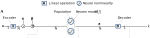
\includegraphics{media/chapters/02_modelling/02_03/nef_representation_diagram.pdf}
	\includegraphics{media/chapters/02_modelling/02_03/nef_representation.pdf}
	{\phantomsubcaption\label{fig:nef_representation_diagram}}
	{\phantomsubcaption\label{fig:nef_representation_current_translation}}
	{\phantomsubcaption\label{fig:nef_representation_tuning_curves}}
	{\phantomsubcaption\label{fig:nef_representation_deocding}}
	\caption[Representation in the Neural Engineering Framework]{Representation in the Neural Engineering Framework. Example for a population of $N = 10$ neurons representing a one-dimensional quantity.
	\textbf{(A)} Schematic overview of the encoding and decoding process.
	\textbf{(B)} Randomly selected affine current translation functions $J_i(\xi) = \alpha_i \langle \vec x, \vec e_i \rangle + J^\mathrm{bias}_i$. The dotted line corresponds to the activity threshold $J_\mathrm{th}$.
	\textbf{(C)} Tuning curves for each neuron in the population after applying the somatic nonlinearity $G[J]$~(eq.~\ref{eqn:lif_response_curve}).
	\textbf{(D)} Reconstructing the represented value from neuron activity by means of linear decoding. Dashed line corresponds to the ideal.}
	\label{fig:nef_representation}
\end{figure}

\subsubsection{Selecting encoders, gains, and biases}
Of course, this raises the question of how modellers should select encoders $\vec e_i$, biases $\beta_i$, and gains $\alpha_i$.
To form a good basis for a population code, the population must exhibit diverse tuning (cf.~\Cref{fig:population_code}).
At the same time, the tuning curves must stay within modelling constraints such as the maximally observed firing rates $a_i$ for the range of stimuli $\vec x$ over which we characterise the neuron population.
We denote the set of represented values as a compact set \Xrepr with finite, non-zero volume $\vol(\Xrepr)$.

Unless more specific data are available, we can for example assume that $\vec x$ are within a hyperball of radius $r$, i.e., $\Xrepr = r \Ball^d$.
The encoding vectors $\vec e_i$ can be sampled from the unit hypersphere $\mathbb{S}^d$.
For monotone increasing response curves $G$, gain $\alpha$ and bias $\beta$ can be computed for each neuron by sampling an \enquote{$x$-intercept} value $\xi_0$ from the interval $[-r, r]$ and a maximum rate $a_\mathrm{max}$.
We then solve for $\alpha$, $\beta$ such that the following equations hold:
\begin{align*}
	\alpha \xi_0 + \beta &= J_0 = G^{-1}[0] \,, &
	\alpha r + \beta &= J_\mathrm{max} = G^{-1}[a_\mathrm{max}] \,, & \text{where } G^{-1}[a] &\coloneqq \max \big\{ J \mid G[J] = a \big\} \,.
\end{align*}
We get $(r - \xi_0) \alpha = J_\mathrm{max} - J_0$, $(r - \xi_0) \beta = (r J_0 - \xi_0 J_\mathrm{max})$.
For example, for each tuning curve in \Cref{fig:nef_representation}, we randomly sampled a $\xi_0$ from a uniform distribution over $[-1, 1]$, and a maximum firing $a_\mathrm{max}$ rate uniformly from $[10, 50]$.

\subsubsection{Computing identity decoders}
\Cref{eqn:encoding} describes the average neural activities $\vec a$ we expect when a population is representing a certain value $\vec x$; that is, this equation describes how quantities $\vec x$ are \emph{encoded} in a neural network.
Complementary to encoding is \emph{decoding}.
That is, given the activities $\vec a$, we would like to reconstruct the represented $\vec x$.
This could---for example---be accomplished using Bayesian inference, as we demonstrated in \Cref{fig:population_code}.
If the number of neurons \Npop in a population is large enough we can, to a very similar effect, just use a linear decoding matrix \Dec (\Cref{fig:nef_representation}; \cite{salinas1994vector}).

The idea is to simply multiply the activities $\vec a$ with a matrix $\Dec \in \mathbb{R}^{d \times \Npop}$ such that the decoded $\vec{\hat x} = \Dec \vec a(\vec x)$ is approximately equal to the encoded $\vec x$, for any $\vec x \in \Xrepr$.
Under the assumption that the activities $\vec a$ are subject to independent and identically distributed (i.i.d.) zero-mean Gaussian noise with standard-deviation $\sigma$, the decoding matrix \Dec can be obtained by minimising a least-squares loss-function $E$:
\begin{align}
	E &= \frac{1}{\vol(\Xrepr)} \iint_{\Xrepr} \bigl\| \vec x - \Dec \bigl( \vec a(\vec x) + \nu \bigr) \bigr\|_2^2  \, \mathrm{d}\vec{x} \quad\quad \text{where } \nu \sim \Normal(0, \sigma) \,.
	\label{eqn:lstsq_loss_identity}
\end{align}
Of course, minimising this integral directly is infeasible.
We approximate a solution numerically by drawing \Nsmpls samples from \Xrepr, denoted $\vec x_1$, $\ldots$, $\vec x_N$.
Arranging the samples and the corresponding population activities in matrices $\mat X = \begin{pmatrix} \vec x_1, \ldots, \vec x_{\Nsmpls} \end{pmatrix} \in \mathbb{R}^{\Nsmpls \times \Ndim}$ and $\mat A = \begin{pmatrix}\vec a(\vec x_1), \ldots, \vec a(\vec x_{\Nsmpls})\end{pmatrix} \in \mathbb{R}^{\Nsmpls \times \Npop}$, we can phrase finding \Dec as a Tikhonov regularised least-squares optimisation problem
\begin{align}
\min_{\Dec} \sum_{k = 1}^{\Nsmpls} \| \Dec \vec a(\vec x_k) - \vec x_k \|_2^2  + \| \sigma \Dec \|^2_\mathrm{F}
&= \min_{\Dec} \| \mat A \Dec^T - \mat X \|_\mathrm{F}^2 + \sigma^2 \Nsmpls \| \Dec \|_\mathrm{F}^2 \,,
\label{eqn:lstsq_loss}
\end{align}
where $\lambda = N \sigma^2$ is the regularisation factor.
From a probabilistic perspective, this particular choice of $\lambda$ results in the exact maximum a-posteriori solution for $\mat D$ with the prior assumption that there is Gaussian noise with standard deviation $\sigma$ on the measurements $\mat A$ \citep[Chapter~6]{boyd2004convex}. 
Larger $\lambda$ increase the robustness of the solution with respect to noise, but decrease the noise-free approximation error.
The solution can be expressed in terms of the regularised Moore-Penrose pseudo-inverse:
\begin{align}
\Dec^T &= \mat A^+ \mat X \,, &\text{where} \quad \mat A^+ &= \bigl(\mat A^T \mat A + \lambda N \mat I \bigr)^{-1} \mat A^T \,.
\label{eqn:decoding}
\end{align}
As explored by \citet[Chapter~2]{eliasmith2003neural}, the decoding error $E$ tends to decrease with $\mathcal{O}(\sqrt{n})$, assuming that the tuning curves have uniform $x$-intercepts and random encoders $\vec e_i$.
An example of this decoding scheme is given in \Cref{fig:nef_representation_deocding}.

Note that, as mentioned before, we do not take dynamics into account when computing the decoders \Dec.
However, as we discuss next, the same \Dec can be used to decode represented values through time in spiking networks when defining activity $\vec a(t)$ as low-pass filtered population spike trains.
We explicitly take temporal aspects of neural computation into account in \Cref{sec:nef_dynamics} below, and when we discuss temporal tuning in Chapter~4.

\pagebreak

\subsection{Principle 2: Transformation}
\label{sec:nef_transformation}

The representation principle maps vectors $\vec x$ onto average neural activities $\vec a(\vec x)$.
Of course, individual neuron populations seldom exist in isolation.
To construct \emph{networks} that realise the desired tuning properties, we need to determine synaptic weights $w_{ij}$ that describe the connection strength between the $j$th pre- and the $i$th post-neuron.
In addition to realising the chosen representations, the \NEF puts a further modelling constraint on the synaptic weights:
\begin{framed}
\noindent\emph{\NEF Principle 2.} Synaptic connections between neural ensembles approximate nonlinear transformations $\vec y = f(\vec x)$, where $\vec x \in \mathbb{R}^d$ is the value represented in the pre-population, and $\vec y \in \mathbb{R}^{d'}$ the value represented in the post-population.
\end{framed}

\begin{figure}
	\centering
	
\includegraphics{media/chapters/02_modelling/02_03/nef_transformation_annotations.pdf}%
	\kern-157.19mm\includegraphics{media/chapters/02_modelling/02_03/nef_transformation.pdf}
	\caption[Examples of the function decoding scheme]{Examples of the function decoding scheme. Instead of decoding the represented value $\vec x$ from a neuron population, we can approximate arbitrary functions $f(\vec x)$.
	\textbf{(A)} $\Npop = 20$ tuning curves $\vec a(x)$; same parameters as in \Cref{sec:nef_representation}. \textbf{(B-E)} Different linear decodings $\mat D^f \vec a(x)$ of the above tuning curves. Dotted line is the target function, thick line the decoded function. Inset $E$ is the \RMSE.
	}
	\label{fig:nef_transformation}
\end{figure}

That is, modellers can choose a transformation $f$ that should be computed in a connection.
We can easily approximate functions $f$ of the value $\vec x$ represented in a pre-population using a \emph{function decoder} $\Dec^f$.
This $\Dec^f$ has the property that $\Dec^f \vec a(\vec x) = \vec{\hat y} \approx \vec{y} = f(x)$.
Modifying the least-squares loss from \cref{eqn:lstsq_loss_identity}, we get
\begin{align}
	E &= \frac{1}{\vol(\Xrepr)} \iint_{\Xrepr} \bigl\| f(\vec x) - \Dec \bigl( \vec a(\vec x) + \nu \bigr) \bigr\|_2^2  \, \mathrm{d}\vec{x} \quad\quad \text{where } \nu \sim \Normal(0, \sigma) \,.
	\label{eqn:lstsq_loss_f}
\end{align}
Analogously to the above, a discrete approximation of $\mat D^f$ for \Nsmpls samples ${\vec x}_1$, $\ldots$, ${\vec x}_{\Nsmpls}$ is given as 
\begin{align*}
	\bigl(\Dec^f\bigr)^T &= \mat A^+ \mat Y \,, &\text{where } \mat A &= \begin{pmatrix}\vec a(\vec x_1), \ldots, \vec a(\vec x_{\Nsmpls})\end{pmatrix} \in \mathbb{R}^{\Nsmpls \times \Npop} \,, & \mat Y &= \begin{pmatrix}f(\vec x_1), \ldots, f(\vec x_{\Nsmpls})\end{pmatrix} \in \mathbb{R}^{\Nsmpls \times \Ndim'} \,.
\end{align*}
Examples of functions decoded from $\vec a(\vec x)$ are depicted in \Cref{fig:nef_transformation}.
The decoding error $E$ depends on the number of pre-neurons \Npop, as well as the \enquote{smoothness} of the decoded function.

\begin{figure}
	\centering
	\vspace{0.25mm}
	\includegraphics{media/chapters/02_modelling/02_03/nef_transformation_diagram.pdf}
	\caption[Neuron populations in the NEF as a single-hidden-layer artificial neural network]{Neuron populations in the \NEF form a single-hidden-layer artificial neural network. Encoders $\mat E$, gains $\vec \alpha$, and gains $\vec \beta$ correspond to a fixed input transformation. The function decoder $\Dec^f$ forms a set of linear output weights. Since the input transformations are fixed, computing $\Dec^f$ is simple.}
	\label{fig:nef_transformation_diagram}
\end{figure}

\subsubsection{Comparison to artificial neural networks}
From the perspective of artificial neural networks, the \NEF characterises neuron populations as a single-hidden-layer neural network with a fixed input transformation defined by the encoders, gains, and biases.
Since the input transformation up to the neural nonlinearity---approximated by the response curve $G[J]$---is fixed, learning the output weights---the function decoder---is a convex optimisation problem and no stochastic optimisation such as gradient descent is required (\Cref{fig:nef_transformation_diagram}).

Similar nonlinear encoding and linear decoding schemes have been explored in machine learning for decades.
One early example are the radial basis function networks described by \citet{broomhead1988radial}.
Going back even further, the overall idea is similar to the pattern-recognition model of granule cell activity in the cerebellum proposed by \citet{marr1969theory}.
From a more theoretical perspective, neuron population tuning-curves $\vec a(\vec x)$ span a function space with a set of non-orthogonal basis functions. 
\citet{hornik1989multilayer} show that---assuming a reasonable distribution of these basis functions---we can approximate any continuous function over \Xrepr to a desired degree by increasing the number of hidden units.
% TODO: Reference to other basis function related stuff

\subsubsection{Computing synaptic weights}
As we have seen, function decoders $\Dec^f$ can approximate arbitrary functions $f$ over \Xrepr.
Of course, this is only half of what we set out to accomplish.
Our goal was to find synaptic weights $\mat W \in \mathbb{R}^{m \times n}$ that connect from a pre-population of \Npop neurons representing $\vec x$ to a post-population of $m$ neurons, such that the tuning properties of the target population are preserved, \emph{and} the post-population is representing a transformed version $f(\vec x)$.

If we assume that the current translation function $J_i(x)$ is an intrinsic part of each post-neuron $i$, encoding and decoding can be linearly combined into a weight vector $\vec w_i$:
\begin{align}
	a_i^\mathrm{post}\bigl(f(\vec x)\bigr)
		&\approx
	a_i^\mathrm{post}\bigl(\mat D^f \vec a_\mathrm{pre}(\vec x)\bigr)
		=	
	G\bigl[J_i\bigl(\langle \vec e_i^T, \mat D^f \vec a^\mathrm{pre}(\vec x)\rangle \bigr)\bigr]
		=
	G\bigl[J_i\bigl(\langle \vec w_i, \vec a^\mathrm{pre}(\vec x) \rangle \bigr)\bigr] \,.
	\label{eqn:nef_weight_vector}
\end{align}
Hence, $\mat W = \mat E \mat D^f$ forms a synaptic weight matrix, where $\mat E \in \mathbb{R}^{m \times d'}$ is a matrix of post-population encoding vectors $\vec e_i$, and $\mat D^f$ is the pre-population function decoder.
This matrix implicitly decodes $\vec{\hat y} = f(\vec x)$ from a pre-population, and re-encodes $\vec{\hat y}$ in the post-population.

%Note that these synaptic weights directly translate the pre-population activities into an average current that is injected into the post-neuron.
%Although biological neural networks do not possess \enquote{encoding} and \enquote{decoding} matrices with intermediate low-dimensional representations, the product $\mat W = \mat E \Dec^f$ has the equivalent effect of first decoding, and then re-encoding.

A welcome side-effect of this formalisation is that the weight matrix $\mat W$ is of low rank.
This significantly reduces the amount of computation required to evaluate \NEF networks.
Consider a matrix-vector product of the form $\mat W \vec a$.
Evaluating this requires $\mathcal{O}(mn)$ operations, where \Npop and $m$ are the number of neurons in the pre- and post-population.
In contrast, multiplying the low-rank factorisation with an activity vector, i.e., computing $\mat E ( \mat D \vec a 
)$, requires only $\mathcal{O}(\Ndim n + \Ndim' m)$ operations.
Since, typically, $d \ll n$ and $d' \ll m$, this is a linear time operation.
Along with the linearity of homogeneous synaptic filters, this enables Nengo to simulate large spiking neural networks on commodity hardware \citep{bekolay2014nengo}.

\subsection{Principle 3: Dynamics}
\label{sec:nef_dynamics}

% TODO: Mention the key-word recurrent somwhere!

\begin{figure}
	\centering
	\includegraphics{media/chapters/02_modelling/02_03/instantaneous_spike_rate.pdf}%
	{\phantomsubcaption\label{fig:instantaneous_spike_rate_a}}%
	{\phantomsubcaption\label{fig:first_order_low_pass}}%
	\caption[Estimating the instantaneous firing rate using a synaptic filter]{Estimating the instantaneous firing rate using a first-order exponential synaptic filter. \textbf{(A)} Blue line depicts a spike train (short black lines at the bottom) filtered by a first-order exponential low-pass filter $h(t)$ with $\tau = \SI{0.1}{\second}$. The black line is the \enquote{ground-truth} rate underlying the spike train (using a $\Delta\Sigma$-modulator).
	Apart from a phase shift and some added noise, the low-pass filtered spike train tracks the ground truth well.
	\textbf{(B)} Visualisation of the synaptic filter $h(t)$. We assume that spikes are Dirac deltas and that the filter has unit DC-gain, i.e., the area under the curve is one.}
	\label{fig:instantaneous_spike_rate}
\end{figure}

So far, and as mentioned several times before, we have ignored the fact that spiking neural networks possess temporal dynamics.
Instead, and very similar to the rate-based artificial neural networks used in machine learning, we assumed average firing rates in the encoding and decoding equations.
Fortunately, this is less of a problem as it may seem.

Synaptic dynamics (cf.~\Cref{sec:synaptic_transmission}) act as a filter that estimates the pre-synaptic \emph{instantaneous firing rate} of a spike train.
The instantaneous firing rate is the spike rate $a_i$ of a neuron at a single point in time $t$.
Of course, this is a quite paradoxical notion.
As mentioned before, by the Fourier uncertainty principle, we cannot measure an event rate without averaging over time; the smaller the time-window, the smaller the frequency resolution (cf.~\cite{gabor1946theory}).

Still, low-pass filters can be reasonably effective at inferring the state of a process generating binary events.
This is illustrated in \Cref{fig:instantaneous_spike_rate}.
The low-pass filtered spike train is clearly centred around the ground-truth rate.
The deviations from the ground-truth can be interpreted as noise.
Conveniently, we already accounted for noise by relying on population codes, and regularising the decoding matrices $\mat D^f$ (eq.~\ref{eqn:lstsq_loss_f}).
More information on this topic can be found in \citet[Chapter~4]{eliasmith2003neural}, as well as later in Chapter~4 of this thesis.
%TODO: Reference to Chapter 4.

Correspondingly, since synaptic filters approximate the instantaneous firing rate, the techniques discussed so far will also work well in the context of spiking neural networks.
However, as discussed above, instead of merely translating mathematical descriptions into spiking neural networks, we would also like to know how resources available in biologically plausible spiking neural networks can \emph{support} high-level function.

In this vein, the third \NEF principle describes how synaptic filters can be exploited to approximate arbitrary dynamical systems.
Paraphrasing \citet{eliasmith2003neural}:
\begin{framed}
	\noindent\emph{\NEF Principle 3.}
	Represented values are state variables $\vec x(t)$ in a dynamical system. Recurrent connections approximate arbitrary dynamical systems of the form $\dot{\vec x}(t) = f(\vec x(t), \vec u(t), t)$, where $\vec x(t)$ is the represented value, $\vec u(t)$ is some external input, and $t$ is time.
\end{framed}

\begin{figure}
	\centering
	
\includegraphics{media/chapters/02_modelling/02_03/nef_dynamics_diagram_ab.pdf}
	{\phantomsubcaption\label{fig:nef_dynamics_integral}}%
	{\phantomsubcaption\label{fig:nef_dynamics_synaptic}}%
	\caption[Integrator and synaptic filter realisations of an LTI system]{Integrator and synaptic filter realisations of an \LTI system. Orange circles depict temporal convolutions.
	\textbf{(A)} The standard \LTI system.
	\textbf{(B)} Using a low-pass filter instead of a perfect integrator.}
	\label{fig:nef_dynamics_ab}
\end{figure}

This principle is best explained considering linear time-invariant (\LTI) systems of the form
\begin{align*}
	\dot{\vec x}(t) &= \mat A \vec x(t) + \mat B \vec u(t) \,,
\end{align*}
where $\mat A \in \mathbb{R}^{\Ndim \times \Ndim}$ is the feedback matrix, and $\mat B \in \mathbb{R}^{\Ndim \times \Ndim'}$ is the input matrix.
Integration yields
\begin{align}
	\vec x(t)
	&=
		\int_0^t \dot{\vec x}(\tau) \,\mathrm{d}\tau + \vec x_0
	=
		\int_0^t \mat A \vec x(\tau) + \mat B \vec u(\tau) \,\mathrm{d}\tau + \vec x_0 \,,
	\label{eqn:lti_integral_equation}
\end{align}
where $\vec x_0$ is the initial state.
Hence, and as illustrated in \Cref{fig:nef_dynamics_integral}, if we have access to an integrator as a computational primitive, we can easily evaluate dynamical systems of this form.
%In practice, such integral equations can be evaluated using some numerical integration method, the simplest (but least powerful) being Euler integration \citep[cf.][Chapter~17]{press2007numerical}.

Unfortunately, biological neural networks do not contain \enquote{perfect} integrators.
Instead, they need to rely on \enquote{leaky} integrators, such as low-pass filters.
It is easy to see why a low-pass filter is a leaky integrator.
The impulse response of an integrator is a step function (i.e., zero for $t < 0$, one for $t \geq 0$).
Similarly, the impulse response $h(t)$ of a first-order low-pass filter jumps to non-zero value at $t = 0$, but in contrast to the integrator, quickly decays (\Cref{fig:first_order_low_pass}).
The key idea of the dynamics principle is to compensate for this \enquote{forgetfulness}.
That is, we change the desired dynamical system to account for leaky integration (\Cref{fig:nef_dynamics_synaptic}).

Despite the name, the \enquote{leaky integrator} dynamics of the \LIF neuron itself are of little use.
The neuron resets its state with every output spike, loosing all the integrated information.
Fortunately, the low-pass filter dynamics of synapses are decoupled from the neural superthreshold dynamics.
Moreover, as explained by
\citet[Chapter~8 \& Appendix~F.1]{eliasmith2003neural},
it is not unreasonable to assume that the synaptic filter dominates the overall neural dynamics.
In other words, dynamics mainly stem from the synaptic filter $h(t)$.
We revisit this assumption in \Cref{sec:nef_limitations} below.

We can easily derive a system that compensates for the low-pass filter dynamics using the Laplace transform.
Assume that both the feedback and the input passes through the same first-order low-pass filter with time-constant $\tau$.
Treating both the integral in \cref{eqn:lti_integral_equation} and the low-pass filter as convolutions with their respective impulse response, we have
\begin{align}
	X(s) &= \frac{1}{s} \bigl( \mat A X(s) + \mat B U(s) \bigr) & \text{and} \quad\quad X(s) &= \frac{1}{1 + \tau s} \bigl( \mat A' X(s) + \mat B' U(s) \bigr) \,.
	\label{eqn:original_vs_modified_lti}
\end{align}
Rearranging the second equation and comparing coefficients to the first equation we get
\begin{align}
	X(s) &= \frac{1}{s} \Big( \frac{\mat A' - \mat I}{\tau} X(s) + \frac{\mat B'}{\tau} U(s) \Big) &
	\leadsto \quad \quad \mat A' &= \tau \mat A + \mat I \,, &
	\mat B' &= \tau \mat B \,.
	\label{eqn:nef_transform_a_b}
\end{align}
For arbitrary dynamics $f(\vec x, \vec u, t)$ we similarly obtain $f'(\vec x, \vec u, t) = \tau f(\vec x, \vec u, t) + \vec x$ \citep[Appendix~B.3]{eliasmith2013how}.
In other words, to compensate for low-pass filter dynamics, we scale the dynamics by $\tau$ and feed back $\vec x$ to \enquote{remind} the system of its current state.

\begin{figure}
	\centering
	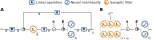
\includegraphics{media/chapters/02_modelling/02_03/nef_dynamics_diagram_c.pdf}%
	{\phantomsubcaption\label{fig:nef_dynamics_neurons_a}}%
	{\phantomsubcaption\label{fig:nef_dynamics_neurons_b}}%
	\caption[Synaptic filters and LTI systems in NEF networks]{Synaptic filters and \LTI systems in \NEF networks.
	\textbf{(A)} \NEF realisation of an \LTI system. Homogeneous synaptic filters are modelled as $d$ filters placed before the encoder.
	\textbf{(B)} Technically, each of the $n \times m$ synaptic connections between a pre- and a post-population has its own synaptic filter. When scaled appropriately, the resulting filter matrix replaces the synaptic weights; however, this has drastically higher computational costs than placing $d$ filters ahead of the encoder.}
	\label{fig:nef_dynamics_neurons}
\end{figure}

Using the representation and transformation principles, we can turn the block-diagram in \Cref{fig:nef_dynamics_synaptic} into a spiking neural network.
This is schematically depicted in \Cref{fig:nef_dynamics_neurons_a}.
The decoded state $\vec{\hat x}$ and the input $\vec u$ are passed through compensated \LTI matrices $\mat A'$ and $\mat B'$, summed, and fed into the synaptic filters.
We provided an example of this in \Cref{fig:nef_overview}.

Of course, as before, the network can, due to linearity, be expanded into biologically plausible synaptic weights and arrays of synaptic filters (\Cref{fig:nef_dynamics_neurons_b}).
Function decoders $\mat D^f$ can be used to support arbitrary nonlinear dynamics, and not just \LTI systems.

\subsection{Some Limitations of the Neural Engineering Framework}
\label{sec:nef_limitations}

To date, the Neural Engineering Framework has seen considerable use in the scientific community (cf.~\Cref{app:nef_literature}).
Nevertheless, the \NEF has a series of shortcomings that limit the biological plausibility of the generated networks, the number of constraints exposed to modellers, and how well resources available on some neuromorphic hardware platforms are utilised.
Resolving these issues could make the \NEF more appealing to a wider group of researchers and contribute to ongoing efforts in cognitive science and neuromorphic computing.

Of course, the following list of limitations is by no means complete.
To the contrary.
One can quite effortlessly identify areas of neuroscience that are not reflected in the \NEF at all---for example nervous system development, or networks of glial cells.
However, as we implied in the beginning this chapter, we think that, as of now, there is too little consensus on these topics to account for them in a general-purpose modelling tool.

Overall, while it is tempting to incorporate as much biological detail as possible into \NEF networks, this is misguided if merely done as an end in itself.
Remember that our goal is to bridge low-level mechanism and high-level function.
This distinguishes \NEF models from \enquote{bottom-up} approaches, that develop mechanistically detailed models of brain circuits, with the hope that the final system---if truthfully describing biology---exhibits some interesting function \citep[cf.][]{komer2016unified}.
We think that, optimally, extensions to the \NEF should expose new low-level detail as a \enquote{computational resource} that can be systematically exploited for high-level function.
At the very least, extensions should expose additional constraints that provide modellers with an opportunity to explore the impact of individual aspects of neurobiological mechanism on high-level function \citep[e.g.,][]{duggins2017incorporating}.
% TODO: Cite Pete's paper when published

%The two main extensions to the NEF we discuss in this thesis---nonlinear dendritic interactions and temporal tuning---fall into the first category, whereas the other extensions provide additional modelling constraints.

\subsubsection{Limitation 1: Current-based synapses}
In our discussion of Principle 2 (\Cref{sec:nef_transformation}), we implicitly assumed that neurons use current-based synapses (cf.~\Cref{sec:simplified_neuron_models}).
As expressed in \cref{eqn:nef_weight_vector}, we model the current injected into the post-neuron as linearly depending on the pre-population activities.
However, as we discussed in \Cref{sec:synaptic_transmission}, synaptic transmission is better modelled in terms of \emph{conductances}, and not currents.
As noted by \citet[Section~2.1.2, p.~35]{eliasmith2003neural}, accounting for conductances adds another layer of nonlinearity to the neuron.
While such nonlinearities have been analysed in the context of the \NEF by \citet[Chapter~4]{tripp2009search} as well as \citet{bobier2014unifying}, this prior work does not propose a systematic method for exploiting synaptic nonlinearities for computation.

Adapting the \NEF to support nonlinear conductance-based synapses would increase compatibility with neuromorphic hardware platforms emulating conductance-based neurons (e.g.,~BrainScaleS; \cite{schemmel2010waferscale}) and allow modellers to more easily constrain models according to neurophysiological parameters, such as synaptic reversal potentials.
Furthermore, individual synapse types (e.g.,~excitatory and inhibitory) act as independent input channels to a neuron.
As we discuss in the next chapter, these input channels interact nonlinearly in the case of multi-compartment neurons, increasing the class of functions that can be approximated using the same number of neurons.


\subsubsection{Limitation 2: Bias currents}
A minor (as we will see) limitation is the assumption that each neuron possess an intrinsic bias current $\beta_i$ (eq.~\ref{eqn:encoding}).
This current is necessary to ensure diverse tuning.
For example, some neurons are active even if no input is present (\enquote{spontaneous} or \enquote{background} activity).
This can be modelled using positive bias currents.

\Citet[Chapter~2; p.~35]{eliasmith2003neural} interpret the bias current as a \enquote{constant input current from the rest of the nervous system}.
While reasonable, this assumption cannot be strictly true.
The mean firing rate of individual populations varies sigificantly over time \citep{okun2012population}; it is not immediately clear how these variations would support constant $\beta_i$.
Hence, an explicit translation of pre-activities into a bias current $\beta_i$ using synaptic connectivity may be preferable.
Depending on the pre-population tuning, this can affect high-level function.


\begin{figure}
	\includegraphics{media/chapters/02_modelling/02_03/granule_jbias_distribution.pdf}%
	{\phantomsubcaption\label{fig:jbias_a}}%
	{\phantomsubcaption\label{fig:jbias_b}}%
	{\phantomsubcaption\label{fig:jbias_c}}%
	{\phantomsubcaption\label{fig:jbias_d}}%
	{\phantomsubcaption\label{fig:jbias_e}}%
	{\phantomsubcaption\label{fig:jbias_f}}
	\caption[Neuron parameter variability only accounts for small bias currents]{Neuron parameter variability only accounts for small bias currents.
	\textbf{(A, B)} Standard \NEF tuning curves and corresponding bias current distribution.
	\textbf{(C)} Empirical data on resting potential $v_\mathrm{rest}$ variations in cerebellar granule cells from \citet[Figure~1b]{chadderton2004integration} with a Gaussian fit.
	\textbf{(D)} Noisy \LIF neuron response curves for resting potentials samples from the empirical distribution. Colours indicated in \emph{(C)}. Other \LIF parameters fit to empirical data at $v_\mathrm{rest} = \SI{-64}{\milli\volt}$ (black crosses; cf.~Figure~1g in Chadderton et al.). Input currents $J$ are subject to Gaussian noise ($\sigma = \SI{10}{\pico\ampere}$). \textbf{(E)} Histogram of bias currents $\beta_i$ having the same average effect as varying $v_\mathrm{rest}$.
	\textbf{(F)}~Tuning curves that can be realised using these bias currents for the target maximum rates.
	Unfortunately, the empirically observed parameters do not result in tuning curve distributions assumed by the \NEF \emph{(A)}.}
	\label{fig:granule_jbias_distribution}
	\vspace*{-0.5em}
\end{figure}

Furthermore, and directly related to Limitation~1, pre-synaptic activity affects synaptic \emph{conductances} and does not directly induce \emph{currents}.
This is particularly problematic since tuning curves with uniform $x$-intercepts tend to require large \emph{negative} bias currents (\Cref{fig:jbias_a,fig:jbias_b}).
It is unclear how such currents should be generated, particularly since the inhibitory synaptic reversal potential $E_\mathrm{I}$ is close to the resting potential $v_\mathrm{rest}$.
Natural neuron parameter variations are insufficient to explain this discrepancy (\Cref{fig:jbias_c,fig:jbias_d,fig:jbias_e,fig:jbias_f}).

\begin{figure}
	\includegraphics{media/chapters/02_modelling/02_03/constrained_weight_matrices.pdf}
	{\phantomsubcaption\label{fig:sparsity_and_dales_principle_a}}%
	{\phantomsubcaption\label{fig:sparsity_and_dales_principle_b}}%
	{\phantomsubcaption\label{fig:sparsity_and_dales_principle_c}}%
	\caption[Constrained connectivity and Dale's principle]{Constrained connectivity and Dale's principle. \emph{Top:} Weight matrix $\mat W$ and (if applicable) factorisation into $\mat E, \mat D$. \emph{Bottom:} Weight histogram relative to the $95$-percentile $P_{95}$. Red indicates inhibitory, blue to excitatory weights. \textbf{(A)}~Typical \NEF weight matrices are dense.
	\textbf{(B)}~$L_1$-regularisation of decoders $\mat D$ increases sparseness, but does so in an uncontrolled manner. Note that $\mat D$ is (relatively speaking) sparser than $\mat W$.
	\textbf{(C)}~Dale's principle imposes an excitatory/inhibitory split on $\mat W$.
	This is difficult when factorising $\mat W$, but one can solve for $\mat W$ directly using nonnegative least-squares (\NNLS).
	}
	\label{fig:sparsity_and_dales_principle}
\end{figure}

\subsubsection{Limitation 3: Constrained connectivity and Dale's principle}
\NEF weight matrices $\mat W = \mat E \mat D$ are typically dense.
That is, they contain few zeros, implying all-to-all connectivity between neurons (\Cref{fig:sparsity_and_dales_principle_a}).
However, in biology, connectivity in the brain can be quite sparse.
For example, as detailed by \citet[Chapter~20]{braitenberg1998cortex}, the likelihood of two neighbouring cortical cells to be connected is less than $90\%$. Similarly, connectivity between Golgi and Granule cells in the cerebellum is highly constrained (cf.~Chapter~5).
% TODO: Add reference to Chapter 5
It may be desirable to give modellers the opportunity to account for these statistics.

A common way to enforce sparsity is to use $L_1$, or \enquote{lasso}, regularisation instead of the $L_2$ regularisation proposed in \cref{eqn:lstsq_loss_identity,eqn:lstsq_loss_f} \citep[Chapter~6]{boyd2004convex}.
However, solving for sparse decoders $\mat D$ in this way has two issues.
First, this process is uncontrolled---na\"ive $L_1$ regularisation does not take biological constraints into account.
Second, for $\Ndim \gg 1$, orthogonality between the encoders and decoders determines sparsity, and not just the sparsity of $\mat D$ (\Cref{fig:sparsity_and_dales_principle_b}).
Both issues mandate more complex regularisation terms.

Another form of constrained connectivity is to account for Dale's principle.
As we discussed before in \Cref{sec:synaptic_transmission}, individual neurons typically act either exclusively excitatorily or inhibitorily. Empirical data suggest that, depending on the modeled brain region, excitatory cells outnumber inhibitory cells by a factor between two and four~\citep{hendry1981sizes,gabbott1986quantitative}.
This imposes a certain structure onto the weight matrix (\Cref{fig:sparsity_and_dales_principle_c}).

\begin{figure}
	\centering
	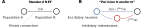
\includegraphics{media/chapters/02_modelling/02_03/parisien_transform.pdf}
	\caption[Illustration of the \enquote{Parisien transform}]{Illustration of the \enquote{Parisien transform}. This transformation accounts for Dale's principle by splitting standard \NEF connections, as depicted in \textbf{(A)}, into an excitatory and inhibitory path \textbf{(B)}.}
	\label{fig:parisien_transform}
\end{figure}

\Citet[Section~6.4]{eliasmith2003neural} propose a method to account for Dale's principle later refined by \citet{parisien2008solving}.
The basic idea of this \enquote{Parisien transform} is to add a specially crafted \enquote{bias function} to the function computed in the excitatory connection.
This bias function ensures that all connection weights are positive.
An inhibitory inter-neuron population is then added to the network and connected in parallel to the excitatory connection to subtract the superfluous current induced by the bias function (\Cref{fig:parisien_transform}).

While mathematically clever, the Parisien transform changes the network structure by adding an inhibitory interneuron population.
Although interneurons are indeed common in brain networks, the connectivity patterns resulting from the Parisien transform may not be desirable.
For example, as we discuss in Chapter~5, Golgi cells are recurrent inhibitory interneurons between granule cells.
However, there are no excitatory recurrent connections between granule cells, as assumed by the Parisien transform.
In the next chapter, we discuss an approach to accounting for Dale's principle that is independent of the network structure.

\subsubsection{Limitation~4: Temporal tuning and neural dynamics}
The dynamics principle derived in \Cref{sec:nef_dynamics} was based on two assumptions.
First, synaptic dynamics dominate neural dynamics.
Second, synaptic filters are homogeneous first-order low-pass filters in both the input and recurrent connection.
While reasonable, these modelling assumptions are, as so often, only coarse approximations of biology.

\begin{figure}[t]
	\includegraphics{media/chapters/02_modelling/02_03/firing_rate_neural_dynamics.pdf}
	\caption[Neural dynamics for different maximum firing rates]{Neural dynamics for different maximum firing rates $a_\mathrm{max}$. A \SI{100}{\second} band-limited white-noise signal $u(t)$ with a band-width of \SI{100}{\hertz} is fed through an \NEF population with uniform $x$-intercepts.
	The transfer function is determined from the decoded $\hat u(t)$ using the method described in \citet[Section~4.3.3]{eliasmith2003neural}.
	We ensure a constant amount of spike noise by setting the number of neurons in the population to $100\,000 / a_\mathrm{max}$. \emph{Top:} Linear transfer function for different maximum rates $a_\mathrm{max}$. \emph{Bottom:} Slice through the transfer functions at the indicated locations.
	\textbf{(A)} Data for a spiking rectified linear unit (\ReLU), a $\Delta\Sigma$-modulator with a rectified input current. This kind of neuron exhibits no significant dynamics of its own, independent of the firing rate. \textbf{(B)} Transfer function for the \LIF neuron. For small firing rates, the neuron acts as a low-pass with a relatively moderate attenuation of about \SI{-5}{\deci\bel}. For firing rates of about \SI{200}{\hertz}, the neuron acts as a pass-through. \textbf{(C)} While similar to the \LIF neuron, the \ALIF
	acts as a very narrow low-pass filter when driven at a maximum firing rate of about \SI{20}{\hertz}. The location of this \enquote{trough} depends on the adaptation time-constant.}
	\label{fig:neural_dynamics_firing_rates}
\end{figure}

The assumption that synaptic dynamics dominate the overall dynamics of a neuron is a good approximation of the behaviour of simple neuron models operating at high firing-rates.
However, for smaller firing rates, the neural dynamics can have a significant impact on the overall system dynamics.
For example, for maximum firing rates below about $\SI{50}{\per\second}$, the sub-threshold low-pass dynamics of the \LIF neuron begin to have a moderate effect on the neural dynamics.
This is depicted in \Cref{fig:neural_dynamics_firing_rates}.

While these rate-dependent effects are relatively small, more complex neuron models possess strong intrinsic dynamics.
For example, the adaptive \LIF (\ALIF) neuron model \citep{camera2004minimal} accounts for firing rate adaptation; that is, each output spike increases the current required to evoke another output spike.
This can be modelled as an inhibitory current resulting from low-pass filtering the neuron's output spike train.
As demonstrated by \citet[Chapter~7]{tripp2009search}, the internal dynamics of the \ALIF neuron model can, under certain circumstances, be exploited to implement arbitrary dynamics using a variant of the equations derived for the \NEF dynamics principle.

The second assumption, namely that synaptic filters are homogeneous, is likely violated if a neuron possesses multiple receptor types.
As we saw in \Cref{sec:synaptic_transmission}, the synaptic time-constant can vary significantly between (and even within) individual receptor types.
We also saw that synaptic transmission is better modelled by higher-order filters.
\Citet{voelker2018improving} discuss methods to generalise the dynamics principle to arbitrary synaptic filters; however, these methods require access to the input signal differentials.

In \Cref{chp:temporal_tuning}, we suggest the concept of \enquote{temporal tuning curves} to---at least partially---account for these issues.
Temporal tuning curves are a direct extension of standard \NEF tuning curves, and are inspired by the concept of temporal receptive fields.
In essence, we treat both synaptic and neural dynamics as temporal resources that can be harnessed to approximate a desired temporal tuning by solving a simple least-squares problem.
This naturally extends the \NEF and, to an extent, unifies the approaches described by Tripp and Voelker systematically.


%
%	\setcounter{chapter}{2}
%	% !TeX spellcheck = en_GB
\chapter{Computational Properties of Multi-Compartment LIF Neurons}

\begin{OpeningQuote}
It may well be that certain nerve pulse combinations will stimulate a given neuron not simply by virtue of their number but also by virtue of the spatial relations of the synapses to which they arrive. This is, one may have to face situations in which there are, say, hundreds of synapses on a single nerve cell, and the combinations of stimulations on these that are effective [...] are characterised not only by their number, but also by their coverage of certain special regions on that neuron [...], by the spatial relations of such regions to each other, and by even more complicated quantiative and geometrical relationships that might be relevant.
\OpeningQuoteSource{John von Neumann}{The Computer and the Brain (1958)}
\end{OpeningQuote}

\begin{PriorPublication}
Portions of this chapter (in particular \Cref{sec:two_comp_lif}) are, in extended and heavily edited form, adapted from \citet{stoeckel2021}, which in turn is an extension of work presented at COSYNE 2018 \citep{stockel2018nonlinear}, as well as an earlier technical report \citep{stockel2017point}.
%Chris Eliasmith supervised this work and edited the manuscripts.
%Aaron Voelker contributed with valuable ideas regarding experimental paradigms during the initial research phase.
Whereas these prior publications focus on single- and two-compartment LIF neurons, we deepen the provided theoretical background and define and discuss $n$-LIF neurons in general.
\end{PriorPublication}

\begin{Contributions}
The work in this chapter can be seen as a continuation of the research presented in \citet[Chapter~5]{koch1999biophysics}, as well as \citet[Chapter~4]{tripp2009search}.
In contrast to these prior publication, we discuss a systematic approach to using passive dendritic nonlinearities as a computational resource to approximate arbitrary functions within the context of functional modelling frameworks.
We particularly focus on convex optimisation, ensuring globally optimal solutions.
Additionally, as far as we are aware, the idea to use quadratic programming for subthreshold relaxation is novel.
\end{Contributions}

As we saw in the previous chapter, individual neurons possess intricate morphologies---a fact, that we mostly ignored for the sake of simplicity.
Indeed, there has been some work incorporating more detailed multi-compartment neuron models into the Neural Engineering Framework \citep{eliasmith2016biospaun,duggins2017incorporating}.
However, these studies merely demonstrate that the NEF is \emph{compatible} with this kind of biological detail.

While reassuring, the---perhaps---more important question to ask is what impact more detailed neuron models have on high-level function.
For example, \citet{duggins2017effects} investigate in how far certain drugs with a known impact on individual neural activity influence the behaviour of entire NEF networks.
Such experimental paradigms could thus, one day, have applications in understanding and treating brain disorders.

From the perspective of computer science, an interesting question to ask is in how far biological detail affects the computations performed by a neuron.

Empirical and theoretical work suggests that the dendritic tree---and not only the soma---is at least partially responsible for the complex responses observed in some biological neurons, including cortical pyramidal cells~\citep{mel1994information,polsky2004computational}.

\citet{london2005dendritic} argue that in addition to active effects in the dendrites (i.e., dendritic spike generation mechanisms), fundamental passive effects such as shunting inhibition are worth being investigated as computational resources.


\begin{itemize}
	\item Motivation. Why should we care about Multi-Compartment LIF Neurons
	\begin{itemize}
		\item Differences to the Bobier attention model and other modeling framework work
		\item Individual neurons as neural networks (e.g., pyramidal cells in cortex)
		\item Available on some neuromorphic hardware platforms; local analogue computation, global digital code.
		\item Multi-channel neurons are useful in general
		\item Can explore effect of 
	\end{itemize}
	\item This we do not model; focus on a viable extension
	\begin{itemize}
		\item Neural dynamics
		\item Dendritic spikes
	\end{itemize}
	\item Overview of this chapter
	\item TODO: How are we harnessing neural dynamics here?
	\item TODO: Contrast spiking neural networks to the rate-mode approximations used at the beginning of this chapter; similar to the way in which we introduced the NEF.
\end{itemize}

%A central challenge in theoretical neuroscience is to describe how biological mechanisms ultimately give rise to behaviour.
%One way to approach this challenge is to build models of neurobiological systems that generate the behaviour of interest to a researcher. Since constructing models that span multiple levels of abstraction is typically difficult, theoretical neuroscientists are working on methods that facilitate mapping high-level behaviour onto neural mechanisms.
%Such modelling frameworks include the Neural Engineering Framework (NEF)~\citep{eliasmith2003neural,eliasmith2013build}, Efficient, Balanced Spiking Networks (EBN)~\citep{boerlin2011spikebased,boerlin2013predictive}, and FORCE~\citep{sussillo2009generating,nicola2017supervised}.
%Generally speaking, these approaches describe how to translate dynamical systems---corresponding to some hypothesized behavioral model---into an idealized spiking neural network that adheres to the desired neurophysiological constraints, for example neural tuning, firing rate distributions, and population-level connectivity ~\citep{komer2016unified,nicola2017supervised}.
%This mechanistic grounding facilitates model validation by enabling a direct comparison of simulation results and empirical data~\citep[e.g.,][]{stewart2012learning,bekolay2014,duggins2017effects,voelker2018improvinga,gosmann2020}.
%
%The frameworks mentioned above primarily rely on two biophysical phenomena as computational primitives: synaptic filtering and the nonlinear relationship between somatic input currents and the neural response. Somatic response models range from leaky integrate-and-fire (LIF) to Hodgkin-Huxley type dynamics~\citep{schwemmer2015constructing,eliasmith2016biospaun,duggins2017incorporating}. Crucially however, these approaches typically assume that post-synaptic currents are a linear superposition of filtered pre-synaptic events. Nonlinear interactions between input channels as they may occur when modelling conductance-based synapses or dendritic structures are typically ignored.
%
%While some research exists that explores the effect of nonlinear post-synaptic currents within these frameworks \citep{bobier2014unifying,thalmeier2016learning,alemi2018learning}, these nonlinearities are seldom systematically exploited. Yet, empirical and theoretical work suggests that active and passive nonlinear effects within the dendritic tree---and not only the soma---are at least partially responsible for the complex responses observed in some biological neurons, including cortical pyramidal cells~\citep{mel1994information,koch1999biophysics,polsky2004computational}. \cite{london2005dendritic} argue that in addition to voltage-gated ionic currents, fundamental passive effects such as shunting inhibition are worth being investigated as computational resources.
%
%Put differently, current functional modelling frameworks only consider a subset of the computational resources available in individual neurons and thus underestimate their computational power. Modellers wishing to multiply two signals might for example be forced to introduce an additional layer of neurons, although---in biology---the interplay between excitation and inhibition within the dendrites of a single neuron layer could have the same effect \citep{koch1999biophysics}. The goal of this paper is to present mathematically tractable methods that allow researchers to take nonlinear post-synaptic currents into account. We demonstrate, as demanded by \cite{london2005dendritic}, that the interactions between passive conductance-based input channels within a single dendritic compartment provide significant computational advantages over standard LIF neurons even within a noisy spiking neural network with low firing rates and small neuron counts.
%
%Specifically, we extend the NEF towards systematically exploiting nonlinear post-synaptic currents. The NEF has been applied to various research areas, including low-level modeling of neurobiological systems~\citep{kuo2005integrating,tripp2009search,bobier2014unifying}, and studying large-scale models of cognitive systems grounded in biology~\citep{eliasmith2012largescale,eliasmith2013build,eliasmith2016biospaun}. A software implementation of the NEF is part of the neural simulation package Nengo~\citep{bekolay2014nengo} and has been used as a neural compiler targeting analog and digital neuromorphic hardware~\citep{choudhary2012silicon,mundy2015efficient,berzish2016realtime,blouw2018benchmarking,neckar2019braindrop}.
%
%The main contributions of this paper are as follows. First, we present a series of extensions to the NEF that improve its compatibility with more biologically detailed neuron models. We describe how to enforce nonnegative weights in conjunction with Dale's principle and extend the NEF towards nonlinear post-synaptic currents, thereby lifting some long-standing limitations of the NEF.
%Second, we derive a post-synaptic current model for a two-compartment leaky integrate-and-fire (LIF) neuron that can be interpreted as a simple dendritic nonlinearity.
%Third, we demonstrate that a single layer of two-compartment LIF neurons can compute a wide variety of functions with an error smaller than or on a par with the accuracy achieved by a comparable two-layer spiking neural network, as long as the target function does not surpass a certain bandwidth.

\clearpage

\section{Theoretical Aspects of Dendritic Computation}
\label{sec:dendritic_computation_theory}

\begin{figure}
	\centering
	
\includegraphics{media/chapter_multi_compartment_lif/nef_multivariate_functions.pdf}%
	{\phantomsubcaption\label{fig:nef_multivariate_functions_a}}%
	{\phantomsubcaption\label{fig:nef_multivariate_functions_b}}%
	{\phantomsubcaption\label{fig:nef_multivariate_functions_c}}%
	\caption[Using dendritic computation to compute multivariate functions in the NEF]{Using dendritic computation to compute multivariate functions in the NEF. \textbf{(A)} Standard NEF networks are additive: summation in activity space corresponds to addition in representation space.
	\textbf{(B)} Computing nonlinear multivariate functions $\phi$ generally requires all variables to be represented in an intermediate population.
	\textbf{(C)} The dendritic computation scheme discussed in here.
	Two pre-populations project onto a post-population with separate excitatory and inhibitory input channels.
	%The nonlinear interaction between these channels is exploited to compute $\phi$.
	}
	\label{fig:nef_multivariate_functions}
\end{figure}

The idea of dendritic computation as pursued here is best explained by exploring how mul\-ti\-va\-ri\-ate functions such as $\phi(x_1, \ldots, x_\ell)$ can be computed in the NEF, and by reviewing some fundamental theoretical properties of neural networks.
Specifically, we analyse three different network architectures (cf.~\Cref{fig:nef_multivariate_functions}).
\enquote{Additive networks} represent the variables $x_1$, $\ldots$, $x_\ell$ in independent neuron populations and cannot approximate most multivariate functions.
In contrast, networks with an intermediate population representing all variables at the same time are universal function approximators.
Dendritic computation relies on non-linear interaction between independent neural input channels.
While not as powerful as networks with an intermediate population, dendritic computation can approximate larger classes of functions well compared to additive networks.

\subsection{Additive Multivariate Networks}
\label{sec:additive_net}

As stated above, our goal is to compute multivariate functions $\phi(x_1, \ldots, x_\ell)$ within the context of the NEF.
%For the sake of simplicity, we mostly discuss bivariate functions of the form $\phi(x_1, x_2)$, but the same considerations apply to more than two input variables as well.
For the sake of simplicity, assume that two pre-populations representing the variables $x_1$, $x_2$ are connected to a common post-population.
To compute $\phi(x_1, x_2)$, we must find connection weights $\vec w_{1, i}$, $\vec w_{2, i}$ such that the following holds for every post-neuron $i$
\begin{align}
	a_i(\phi(x_1, x_2))
		= G_i \bigl[
			\langle \vec e_i, \phi(x_1, x_2) \rangle
		\bigr]
		\supposedEq G_i\bigl[
			\langle \vec w_{1, i}, \vec a^\mathrm{pre}_1(x_1) \rangle + \langle \vec w_{2, i}, \vec a^\mathrm{pre}_2(x_2)
		\rangle\bigr] \,.
	\label{eqn:nef_multivariate_addition}
\end{align}
Here, $a_i$ is the desired post-neuron activity according to the normative tuning-curve constraint (eq.~2.??).
% TODO: Add correct reference
As discussed in the context of the NEF transformation principle in Section~2.3.5, we assume that the current-translation function $J_i$ is part of the individual neuron response curve $G_i$, and that the currents induced by the pre-populations are summed.
% TODO: Add correct reference

Now, consider multivariate functions that can be decomposed into a sum of two univariate functions, i.e., $\phi(x_1, x_2) = f_1(x_1) + f_2(x_2)$ (\Cref{fig:nef_multivariate_functions_a}).
We can easily find weights $\vec w_{1, i}$, $\vec w_{2, i}$ that approximate such a function using the encoder-decoder split of the NEF.
Computing function decoders $\mat D^{f_1}$, $\mat D^{f_2}$ and using the identity $(\vec w_i)^T = \vec e_i \mat D$, we have
\begin{align*}
	G_i\bigl[
	  \langle
	  	\vec e_i \mat D^{f_1},
	  	\vec a^\mathrm{pre}_1(x_1)
	  \rangle
	+ \langle
	  	\vec e_i \mat D^{f_2},
		\vec a^\mathrm{pre}_2(x_2)
	\rangle\bigr] = 
	G_i\bigl[\langle \vec e_i, \mat D^{f_1} \vec a_1^\mathrm{pre}(x_1) + \mat D^{f_2} \vec a_2^\mathrm{pre}(x_2) \rangle\bigr]
	\approx a_i\bigl(f_1(x_1) + f_2(x_2)\bigr) \,.
\end{align*}
This equation can be interpreted as saying that addition in activity space (i.e., summing weighted pre-activities, eq.~\ref{eqn:nef_multivariate_addition}) is equal to addition in represented space.
In other words, standard NEF networks are \emph{additive}.
%\footnote{We already used the additivity of NEF networks in~Section~2.3.5, when we discussed the dynamics principle.}
Summing functions incurs no additional decoding error.

\begin{figure}
	\centering
	
\includegraphics{media/chapter_multi_compartment_lif/perceptron.pdf}%
	{\phantomsubcaption\label{fig:perceptron_a}}%
	{\phantomsubcaption\label{fig:perceptron_b}}%
	\caption[Additive networks are a generalisation of the perceptron]{Additive networks are a generalisation of the perceptron. \textbf{(A)} An additive network is a sum of arbitrary univariate functions. \textbf{(B)} A perceptron is an additive network with functions of the form $f_i(x_i) = w_i x_i + \beta \ell^{-1}$. The weights $w_i$ are learned such that the output approximates a desired function.}
\end{figure}

\subsubsection{Additive networks cannot compute most multivariate functions}
The only way to compute general multivariate functions $\phi(x_1, x_2)$ in additive networks is to \emph{approximate} $\phi$ as an additive univariate decomposition.
As expressed by the following theorem (see Appendix~B.3.1 for a proof), it is \emph{impossible} to compute many continuous multi-variate $\phi$ using such additive networks.%
\footnote{We limit Theorem~\ref{thm:xor_general} to continuous functions for the sake of simplicity.
However, we conjecture that the same results hold for larger classes of functions, for example square Lebesgue integrable functions.}
This is true even if we can decode arbitrary univariate functions $f_1$, $\ldots$, $f_\ell$ over the pre-variables (this is equivalent to having an infinite number of pre-neurons, see below), and we were able to freely choose a fixed nonlinearity $\sigma$ (cf.~\Cref{fig:perceptron_a}).

\begin{theorem}
\label{thm:xor_general}
Let $\ell > 1$, $\Xrepr \subset \mathbb{R}^\ell$ and $\mathbb{Y} \subset \mathbb{R}$ be compact sets, and $\sigma$, $\phi$, $f_i$ be continuous.
For any fixed $\sigma : \mathbb{R} \longrightarrow \mathbb{Y}$, there always exist $\phi : \Xrepr \longrightarrow \mathbb{Y}$ such that there are no $f_1$, $\ldots$, $f_\ell : \mathbb{R}  \longrightarrow \mathbb{R}$ with the property
$\phi(x_1, \ldots, x_\ell) = \sigma(\xi) = \sigma\bigl( f_1(x_1) + \ldots + f_\ell(x_\ell) \bigr)$ for all $(x_1, \ldots, x_\ell) \in \Xrepr$.
\end{theorem}

\begin{figure}
	\centering
	\includegraphics{media/chapter_multi_compartment_lif/xor_visualisation.pdf}%
	{\phantomsubcaption\label{fig:xor_visualisation_a}}%
	{\phantomsubcaption\label{fig:xor_visualisation_b}}%
	{\phantomsubcaption\label{fig:xor_visualisation_c}}%
	{\phantomsubcaption\label{fig:xor_visualisation_d}}%
	{\phantomsubcaption\label{fig:xor_visualisation_e}}%
	\caption[Visualisation of the XOR decision problem for different classifiers]{Visualisation of the XOR decision problem for different classifiers. The goal is to find classifier parameters such that the four samples are classified as depicted.
	The background corresponds to the sign of the monotonic function $\sigma(\xi)$.
	\textbf{(A)} The linear decision boundary formed by the Perceptron cannot solve the XOR problem.
	\textbf{(B)} This holds for any function of the form $\sigma(f_1(x_1) + f_2(x_2))$, here $f_1(x_1) = \cos(2\pi x_1)$ and $f_2(x_2) = \sin(2\pi x_2)$.
	\textbf{(C)} A multi-layer Perceptron (MLP) of the form $\sum_i w_i \sigma(e_i^1 x_1 + e_i^2 x_2 + \beta_i )$ can solve the problem, although the decision boundary is quite erratic.
	\textbf{(D)} An alternative solution using the nonlinearity $\sigma'(\xi) = \sigma(\xi^2 - 1)$.
	\textbf{(E)} Multiplication of two real-valued variables $x_1$, $x_2$ can be seen as a continuous form of the XOR problem.
	Additive networks cannot compute this function.
	}
	\label{fig:xor_visualisation}
\end{figure}

\subsubsection{The Perceptron and XOR}
Consider monotonic $\sigma$ and affine $f_i$ of the form $w_i x_i + \beta \ell^{-1}$.
We obtain the \emph{perceptron}, an early single-layer neural network (cf.~\Cref{fig:perceptron_b}; \cite{rosenblatt1958perceptron}).
\Citet[Chapter~2; originally published in 1969]{minsky1987perceptrons} point out that such networks cannot compute the boolean XOR function (\Cref{fig:xor_visualisation_a}).%
\footnote{\Citet{minsky1987perceptrons} note that the perceptron was proved by Rosenblatt to \enquote{learn to do anything it was possible to program it to do}; this ambiguous statement endowed researchers with a surplus of optimism---especially since perceptrons could sometimes learn to solve difficult problems.
Among other factors, realising that these networks could not be \emph{programmed} to solve a simple problem such as XOR led to what some call \enquote{the first AI winter} \citep[e.g.,][]{muthukrishnan2020brief}.}
%In the continuous domain, the same is true for multiplication over $\mathbb{X} = [-1, 1]^2$, that is $\phi(x_1, x_2) = x_1 x_2$ (\Cref{fig:xor_visualisation_a}).
Even the general additive networks from our theorem cannot solve a \emph{weaker} version of the XOR problem, formalised below.

\begin{definition}
\label{def:weak_xor}
A function $\phi(x, y)$ solves the \emph{weak XOR problem} if there exist $a_0, b_0, a_1, b_1$ with
\begin{align*}
	\big( \phi(a_0, b_0) < \phi(a_0, b_1) \big) \wedge
	\big( \phi(a_1, b_1) < \phi(a_0, b_1) \big) \wedge
	\big( \phi(a_0, b_0) < \phi(a_1, b_0) \big) \wedge
	\big( \phi(a_1, b_1) < \phi(a_1, b_0) \big) \,.
\end{align*}
\end{definition}
That is, we merely require $\phi(a_0, b_0)$ and $\phi(a_1, b_1)$ to be larger than $\phi(a_0, b_1)$ and $\phi(b_1, b_0)$.

\begin{restatable}{theorem}{ThmWeakXor}
\label{thm:weak_xor}
Let $\sigma$ be monotonic. Then, an additive network of the form $\phi(x_1, x_2) = \sigma(f_1(x_1) + f_2(x_2))$ cannot solve the weak XOR problem.
\end{restatable}
This may be surprising, given that, as depicted in \Cref{fig:xor_visualisation_b}, we can generate highly nonlinear classification boundaries.
We provide a proof in Appendix~B.3.2.

To solve the XOR problem, we can either, as discussed next, use multi-layer networks (cf.~\Cref{fig:xor_visualisation_c}), or, alternatively make $\sigma$ non-monotonic.
As depicted in \Cref{fig:xor_visualisation_d}, setting $\sigma(\xi) = \xi^2 - 1$ allows us to solve the XOR problem.
This illustrates our goal with dendritic computation: exploit \enquote{more powerful} $\sigma$ to approximate a larger class of functions.

Still, the functions that we can compute using additive networks are limited, even if we can freely choose $\sigma$.
For example, we can compute $x_1 x_2$ for $(x_1, x_2) \in [\epsilon, 1]^2$ and $0 < \epsilon < 1$ by setting $f_1$ and $f_2$ to the logarithm and $\sigma$ to the exponential.
However, it is impossible to find functions that compute multiplication over all four quadrants---which can be seen as a continuous version of the XOR problem (\Cref{fig:xor_visualisation_e}).
More precisely, allowing $x_1$, $x_2$ to be zero makes it impossible to compute multiplication in these networks (proof in Appendix~B.3.3).
\begin{restatable}{theorem}{ThmMultiplication}
\label{thm:multiplication}
There are no continuous, real-valued functions $f_1$, $f_2$, $\sigma$ such that $\sigma(f_1(x_1) + f_2(x_2)) = x_1 x_2$ for all $(x_1, x_2) \in [0, 1]^2$.
\end{restatable}


%Choosing this $\sigma$ implicitly introduces a non-linear interaction between the variables $x_1$, $x_2$, for example
%\begin{align*}
%	\sigma\left( (w_1 x_1 + w_2 x_2 + \beta)^2 - 1\right) = 
%	\sigma\left( w_1^2 x_1^2 + w_2^2 x_2^2 + 2 w_1 w_2 x_1 x_2 + 2 w_1 \beta x_1 + 2 w_2 \beta x_2 + \beta^2  - 1\right) \,.
%\end{align*}
%The product-term $w_1 w_2 x_1 x_2$ can be exploited to %compute multiplication-like functions.
%Still, as stated in Theorem~1, there inevitably is a large set of functions that we cannot compute.
% TODO Add reference

\subsection{Multi-Layer Networks}

\begin{figure}
	\includegraphics{media/chapter_multi_compartment_lif/mlp.pdf}
	\caption[Sketch of a two-layer neural network]{Sketch of a two-layer neural network with rectified linear units (ReLUs). If the encoding vectors $\vec e_i$ and the biases $\beta_i$ are sampled appropriately, this network is a universal function approximator.}
	\label{fig:mlp}
\end{figure}

As already mentioned in Section~2.3.5, an individual NEF population can be interpreted as a two-layer neural network (cf.~\Cref{fig:mlp}).
% TODO: Add reference
As long as the encoding vectors are sampled from $\ell$-dimensional hypersphere and $x$-intercepts are uniformly distributed, such a neuron population is a universal function approximator.
The following theorem states this more formally for neurons with a rectified linear unit (ReLU) nonlinearity, i.e., $\sigma(\xi) = \max\{0, \xi\}$.

\begin{theorem}
\label{thm:two_layer_universal}
Let $\ell \geq 1$, and $\phi : \mathbb{B}^\ell \longrightarrow \mathbb{R}$ be a continuous function mapping from the $\ell$-dimensional unit ball onto $\mathbb{R}$.
Furthermore, let $\sigma(\xi) = \max\{0, \xi\}$, $\vec e_i$ be sampled uniformly from the unit-sphere $\mathbb{S}^\ell$, and $\beta_i$ be sampled uniformly from $[-1, 1]$.
There exist $d_i \in \mathbb{R}$ such that
\begin{align}
	\phi(\vec x) = \lim_{\Npop \to \infty} \sum_{i = 1}^{\Npop} d_i \sigma\bigl( \langle \vec e_i, \vec x \rangle + \beta_i \bigr) \quad \text{for all} \quad \vec x \in \mathbb{B}^\ell \,.
	\label{eqn:two_layer_network}
\end{align}
\end{theorem}

This follows from \citet{hornik1989multilayer}.
We provide a sketch of a proof in Appendix~B.3.3.
This theorem can be easily extended to hold for arbitrary compact domains $\Xrepr$, codomain dimensionalities, and other neural nonlinearities $\sigma$.

%It may not be obvious why \cref{eqn:two_layer_network} describes a \enquote{two-layer} neural network.
%In essence, the encoding weights $\vec e_i$ map $\vec x$ onto the input of one of the $N$ neurons with nonlinearity $\sigma$.
%This step forms the \enquote{first} or \enquote{hidden layer}.
%The decoding weights $d_i$ then map the neural activities $\sigma(\xi_i)$ onto the output, which forms the \enquote{second layer} (cf.~Figure~2.20).
%% TODO: Add actual reference

\subsubsection{The role of uniformly sampled encoders}
Theorem~\ref{thm:two_layer_universal} requires that the encoding vectors $\vec e_i$ are uniformly sampled from the hypersphere $\mathbb{S}^\ell$.%
\footnote{As follows from the proof of Theorem~\ref{thm:two_layer_universal} in Appendix~B.3.3, there technically are weaker requirements for this.
One example is given in \citet{gosmann2015precise}; given a specific function $\phi$ (such as multiplication), there are certain distributions of encoding vectors that minimise the decoding error.
In fact, global optimisation methods such as stochastic gradient descent can be seen as systematically selecting such \enquote{optimal} encoders.}
To get an intuition as for why this is important, consider the case where the $\vec e_i$ are axis-aligned, i.e., $\|\vec e_i\|_0 = 1$ (cf.~Appendix~A.1).
% TODO: Add reference for zero-norm in Appendix~A.1
In this case, we can split \cref{eqn:two_layer_network} into $\ell$ sub-networks, each decoding a function over a single variable $x_\ell$
\begin{align*}
		\sum_{i = 1}^N d_i \sigma\bigl( \langle \vec e_i, \vec x \rangle - \beta_i \bigr)
	= 	\sum_{j = 1}^\ell \sum_{i = 1}^{N_j} d_{j i} \sigma\bigl( e_{j i} x_j - \beta_{j i} \bigr) \,, \text{where } e_{j i} \in \{ -1, 1\} \,.
\end{align*}
This is equivalent to the additive networks we discussed before.
We can only decode sums of univariate functions over the individual $x_j$ from the pre-population.

\subsubsection{Intermediate populations}
%We now know that we can indeed approximate multivariate functions in the NEF with an arbitrarily small error.
%The pre-condition for this is that all variables over which we would like to compute a $\phi$ represented in the same neuron population with non-axis aligned encoding vectors $\vec e_i$.
As discussed by \citep[Chapter~6]{eliasmith2003neural}, we need to introduce intermediate populations if, as an example, variables $x_1$, $x_2$ are represented in independent pre-populations, and we would like to compute a multivariate function $\phi(x_1, x_2)$.
This intermediate population represents a vectorial quantity $\vec z = (x_1, x_2)$ (cf.~\Cref{fig:nef_multivariate_functions_b}).
This can be accomplished by computing the univariate functions $f_1(x_1) = (x_1, 0)$ and $f_2(x_2) = (0, x_2)$ in the connections to the intermediate population.
According to Theorem~\ref{thm:two_layer_universal} we can then decode any multivariate function from the intermediate population.

\subsubsection{Potential issues with intermediate populations}
In theory, the number of neurons required to cover a $d$-dimensional space is exponential in $d$.
Representing a $d$-dimensional quantity in an intermediate population thus requires many neurons to achieve a certain decoding error.
In practice, it is quite difficult to judge the number of neurons required to decode a certain function $f$ a-priori; the decoding error heavily depends on $f$ and the encoding vectors $\vec e_i$.

Another problem arises when modelling neurobiological systems.
There may be no indication that an intermediate population exists in a particular biological circuit, but the function can be modelled well as a multivariate function.
An example of this would be the aforementioned attention system, where a group of control neurons modulates another population without an intermediary \citep{bobier2014unifying}.

Finally, there is the issue of noise.
In spiking neural networks, every intermediate neuron population introduces additional noise due to static distortion and spike noise \citep[Section~2.2.2]{eliasmith2003neural}.
We see the effects of this later.

\subsection{Dendritic Computation}
\label{sec:dendritic_computation_theory_dendritic}

Dendritic computation is one way to partially alleviate the limitations arising from intermediate populations.
The basic idea is that each neuron possesses $k$ \emph{input channels}.
Input fed through these channels interacts nonlinearly, modelling information processing within the dendrites.

\begin{figure}
	\includegraphics{media/chapter_multi_compartment_lif/dendritic_computation.pdf}%
	{\phantomsubcaption\label{fig:dendritic_computation_net}}%
	{\phantomsubcaption\label{fig:dendritic_computation_fun}}%
	\caption[Overview of our notion of dendritic computation.]{Overview of our notion of dendritic computation. \textbf{(A)} Neuron with an excitatory and inhibitory input channel. In a network context, these functions are decoded from pre-populations representing these variables. Connectivity can be constrained such that excitatory and inhibitory pre-neurons only connect to the corresponding channel. \textbf{(B)} Conceptually, each channel receives a sum of univariate functions computed over the pre-variables $x_1$, $\ldots$, $x_\ell$.}
\end{figure}

Mathematically, the response curve describing the average neural activity is now a multivariate function $\mathscr{G}[\xi_1, \ldots, \xi_k]$, where the $\xi_i$ are linear combinations of the pre-activities (\Cref{fig:dendritic_computation_net}).
To compute $\phi(x_1, \ldots, x_\ell)$, the following must hold for each post-neuron $i$
\begin{align}
	\begin{aligned}
	a_i\bigl(\phi(x_1, \ldots, x_\ell)\bigr) &\supposedEq
	\mathscr{G} \bigl[
		\langle \vec w_{1, i}^1, \vec a^\mathrm{pre}_1(x_1) \rangle + \ldots +
		\langle \vec w_{\ell, i}^1, \vec a^\mathrm{pre}_\ell(x_\ell) \rangle, \ldots,\\
%	&~\quad\quad\vdots, \\
	&~\hspace{1.66em}
		\langle \vec w_{1, i}^k, \vec a^\mathrm{pre}_1(x_1) \rangle + \ldots +
		\langle \vec w_{\ell, i}^k, \vec a^\mathrm{pre}_\ell(x_\ell) \rangle
	\bigr]
	\end{aligned}
	\label{eqn:dendritic}
\end{align}
where $a_i(\phi(x_1, \ldots, x_\ell))$ expresses the normative tuning constraint defined in Section~2.3.2.
% TODO: Add correct reference

Note that we deliberately left the concept of an \enquote{input channel} a little vague.
An input channel could either refer to a different location in the dendritic tree, different synapse types (e.g., excitatory or inhibitory synapses), or even the effects of signalling molecules such as hormones.
We discuss examples of model neurons with multiple input channels in \Cref{sec:nlif}.

\subsubsection{Mathematical analysis}
More formally, using $\sigma(\xi_1, \ldots, \xi_\ell)$ as an abstract nonlinearity and assuming that we can compute any univariate function $g_i^j$ over $\xi_1, \ldots, \xi_\ell$, we have (\Cref{fig:dendritic_computation_fun})
\begin{align}
	\sigma \bigl(
		g_{1}^1(x_1) + \ldots + g_{\ell}^1(x_\ell), \ldots, g_{1}^k(x_1) + \ldots + g_{\ell}^k(x_\ell)
	\bigr) = \phi(x_1, \ldots, x_\ell) \,.
	\label{eqn:dendritic_computation_theory}
\end{align}
Such networks are more powerful than additive networks.
For example, let $\sigma(\xi_1, \xi_2) = \xi_1 \xi_2$.
Now, if we set the functions feeding into the second channel to one, i.e., $g_{1, i}^2(x_1) = \ldots = g_{\ell, 1}^2(x_\ell) = 1$, we obtain an additive network.
Of course, using the same $\sigma$, we can, in contrast to additive networks, compute products of the pre-variables over arbitrary domains.

Still, independent of $\sigma$, and similarly to additive networks, dendritic computation networks are not universal function approximators (see Appendix~B.3.5~for the theorem and proof).

%\begin{theorem}
%\label{thm:dendritic_compuation_incomplete}
%Let $\ell > 1$, $\Xrepr \subset \mathbb{R}^\ell$ and $\mathbb{Y} \subset \mathbb{R}$ be compact sets, and $\sigma$, $\phi$, $g^j_i$ be continuous.
%For any fixed $\sigma : \mathbb{R}^k \longrightarrow \mathbb{Y}$, there always exist $\phi : \Xrepr \longrightarrow \mathbb{Y}$ such that there are no $g^1_1$, $\ldots$, $g^k_\ell : \mathbb{R}  \longrightarrow \mathbb{R}$ with the property
%$\phi(x_1, \ldots, x_\ell) = \sigma(\xi_1, \ldots, \xi_k) = \sigma\bigl( g^1_1(x_1) + \ldots + g^1_\ell(x_\ell), \ldots,  g^k_1(x_1) + \ldots + g^k_\ell(x_\ell)\bigr)$ for all $(x_1, \ldots, x_\ell) \in \Xrepr$.
%\end{theorem}

%\subsubsection{Interaction between excitation and inhibition}
%\Cref{fig:nef_multivariate_functions_c} shows an example of a neural network exploiting nonlinear interactions between excitatory and inhibitory synapses.
%Assume that each neuron in the post population possesses an independent excitatory and inhibitory channel, and that the two pre-population represent $x_1$, $x_2$, respectively, and project onto both channels.
%The activity of a single post-neuron $i$ is hence given as
%\begin{align*}
%	\mathscr{G}_i\bigl[
%		\langle
%			\vec w^1_\mathrm{E},
%			\vec a_\mathrm{pre}^1(\vec x_1)
%		\rangle + \langle
%			\vec w^2_\mathrm{E},
%			\vec a_\mathrm{pre}^2(\vec x_2)
%		\rangle,
%		\langle
%			\vec w^1_\mathrm{I},
%			\vec a_\mathrm{pre}^1(\vec x_1)
%		\rangle + \langle
%			\vec w^2_\mathrm{I},
%			\vec a_\mathrm{pre}^2(\vec x_2)
%		\rangle
%	\bigr] \,,
%\end{align*}
%where $\vec w_\mathrm{I}$ and $\vec w_\mathrm{E}$ are the excitatory and inhibitory synaptic weights, and $\vec a_\mathrm{pre}$ are the activities of the pre-populations.
%Assuming that we can decode arbitrary univariate functions over $x_1$, $x_2$ from the pre-populations, our goal is to find functions $g_\mathrm{E}^1(x_1)$, $g_\mathrm{E}^2(x_2)$, $g_\mathrm{I}^1(x_1)$, $g_\mathrm{I}^2(x_2)$, such that the total activity of our neuron has some desired value, i.e.,
%\begin{align*}
%	a_i^\mathrm{post}(\phi(x_1, x_2)) \supposedEq \mathscr{G}_i\bigl[
%		g_\mathrm{E}^1(x_1) + g_\mathrm{E}^2(x_2),
%		g_\mathrm{I}^1(x_1) + g_\mathrm{I}^2(x_2)
%	\bigr] \,.
%\end{align*}


\subsection{Numerical Exploration}
\label{sec:dendritic_computation_theory_numerical}

The above considerations are quite theoretical and provide only limited insight into the practical impact of choosing one network type over the other.
In this section, we discuss a simple numerical experiment that highlights the function approximation errors obtained with different network types for functions $\phi$ of varying \enquote{complexity}.
We use experiments similar to the following throughout this chapter to characterise different network- and neuron-types.

\begin{figure}
	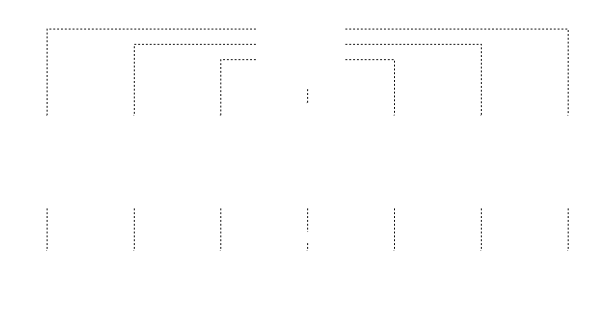
\includegraphics{media/chapter_multi_compartment_lif/2d_functions_overview_overlay.pdf}%
	\kern-157.24mm\includegraphics{media/chapter_multi_compartment_lif/2d_functions_overview.pdf}
	\caption[Overview of our procedure for generating random 2D functions]{Overview of our procedure for generating random 2D functions. \textbf{(A)} We sample a 2D array from a normal distribution (size of the array depends on the filter width; negative values in red, positive in blue). \textbf{(B)} The noise is filtered by convolving with a Gaussian kernel with standard-deviation $\sigma$ (for large filter widths, i.e., small $\sigma^{-1}$, only a small portion of the filter is depicted). \textbf{(C)} The resulting functions are transformed to have mean zero (i.e., no DC component) and a standard deviation of one.}
	\label{fig:2d_functions_overview}
\end{figure}

To analyse different network architectures, w
e randomly generate two-dimensional functions $\phi(x_1, x_2)$ from band-limited white noise with standard deviation one and mean zero.
The band-limit is enforced by filtering with a Gaussian filter kernel with standard deviation $\sigma$.
This is depicted in \Cref{fig:2d_functions_overview}.
Large $\sigma$ result in functions with no high frequencies; such functions are approximately linear.
In contrast, small $\sigma$ result in quite intricate random structures.
Correspondingly, $\sigma^{-1}$ can be seen as a proxy for the \enquote{complexity} of a function.
Small $\sigma^{-1}$ result in low-complexity functions, large $\sigma^{-1}$ in high-complexity functions.


\clearpage

\section{Extending the Neural Engineering Framework}

Up to this point, we have formally defined dendritic computation and discussed its theoretical benefits.
The goal of this section is to open avenues toward systematically integrating multi-compartment neuron models with dendritic trees into NEF networks using the formalisms discussed above.

Na\"ively, incorporating neurons with multiple nonlinear input channels into the NEF is merely a matter of solving for $\vec w$ such that \Cref{eqn:dendritic} holds.
Phrasing this as an optimization problem, we must minimise the difference between the desired average activity according to the normative tuning-curve constraint $a_i(\vec x)$ and the average activity according to our multi-variate response curve $\mathscr{G}$.
Using a least-squares loss (and omitting the regularisation term), we have
\begin{align}
	\begin{aligned}
	E &=
	\frac{1}{\vol(\Xrepr)} \int_{\Xrepr} \Bigl( a_i\bigl(\phi(x_1, \ldots, x_\ell)\bigr) -
	\mathscr{G} \bigl[
		\langle \vec w_{1, i}^1, \vec a^\mathrm{pre}_1(x_1) \rangle + \ldots +
		\langle \vec w_{\ell, i}^1, \vec a^\mathrm{pre}_\ell(x_\ell) \rangle, \ldots,\\
	&~\hspace{13.825em}
		\langle \vec w_{1, i}^k, \vec a^\mathrm{pre}_1(x_1) \rangle + \ldots +
		\langle \vec w_{\ell, i}^k, \vec a^\mathrm{pre}_\ell(x_\ell) \rangle
	\bigr] \Bigr)^2 \,dx_1 \ldots dx_\ell \,.
	\end{aligned}
	\label{eqn:dendritic_computation_optimisation}
\end{align}
On way to minimise this loss-function would be to use stochastic gradient descent.
In fact, this can be a viable strategy---and may be the only option for many detailed neuron models.

Still, we would like to suggest a more systematic approach that, in some cases, reduces the task of finding weights to a convex quadratic program.
This is more in line with the \enquote{standard} NEF, where connection weights are computed by solving a convex least-squares problem.

To arrive at a point where we can integrate complex neuron models more seamlessly, we first need to address two of the limitations of the NEF discussed in Section~2.3.5.
Specifically, we discuss how to eliminate the bias currents and to account for Dale's principle.
Furthermore, we present a modified version of \Cref{eqn:dendritic_computation_optimisation} that splits the multivarite response-curve $\mathscr{G}$ into a multivariate input-dependent nonlinearity $H$ and a univariate response-curve $G$.
We avoid decoding subthreshold currents using a technique we call \enquote{subthreshold relaxation}.

\subsection{Decoding the Current-Translation Function}
\label{sec:nef_decode_current}

So far we assumed that the current translation function $J_i(\xi)$ is an intrinsic part of the neuron model.
Our typical choice of $J_i(\xi) = \alpha_i \xi + \beta_i$ introduces a bias current $\beta_i$ into each neuron.
As we elaborated in Section~2.3.5, this is slightly implausible from a biological perspective.

\Citet{tripp2007neural} demonstrate that it is possible to robustly solve for synaptic weights that approximate arbitrary post-synaptic current functions.
We use this insight to directly approximate the target current $J_i(\langle \vec e_i, \vec x \rangle)$ and thus implicitly solve for the bias.
Again, assuming that the post-synaptic current is linear in the pre-population activities, we must find a weight vector $\vec w_i$ such that the following regularised loss is minimised
\begin{align}
E = \frac{1}{\vol(\Xrepr)} \int_{\Xrepr} \left( J_i\bigl(\langle \vec e_i, \phi(\vec x)\rangle\bigr) - \langle \vec w_i, \vec a^\mathrm{pre}(\vec x) \rangle \right)^2 \, d\vec x + \lambda \| \vec w_i \|_\mathrm{2}^2\,.
\label{eqn:decode_current}
\end{align}
As before, this equation can be discretised and brought into canonical least squares form and solved using the regularised Moore-Penrose pseudo inverse (cf.~eqn.~2.22 and 2.23):
\begin{align*}
	\mat W &= \mat A^+ \mat J \,, & \text{where} \quad \mat A^+ &= (\mat A^T \mat A + \lambda N \mat I)^{-1} \mat A^T \,.
\end{align*}
Here, $N$ is the number of samples, $\mat W \in \mathbb{R}^{m \times \Npop}$ is the connection weight matrix, $\mat J \in \mathbb{R}^{N \times m}$ is a matrix of target currents, and $\mat A \in \mathbb{R}^{N \times n}$ is the matrix of pre-activities.

\begin{figure}
	\includegraphics{media/chapter_multi_compartment_lif/current_translation_decoding.pdf}%
	{\phantomsubcaption\label{fig:current_translation_decoding_a}}%
	{\phantomsubcaption\label{fig:current_translation_decoding_b}}%
	{\phantomsubcaption\label{fig:current_translation_decoding_c}}%
	{\phantomsubcaption\label{fig:current_translation_decoding_d}}%
	\caption[Decoding for currents instead of represented values]{Decoding for currents instead of represented values. \textbf{(A)} Tuning curves of a pre-populations with $100$ LIF neurons (only $50$ tuning curves are shown). \textbf{(B)} Decoding affine current translation functions $J_i$ (black dotted lines are the target). The function $\phi$ being computed in re\-pre\-sen\-tat\-ion space is the identity function. Dashed line corresponds to the threshold current $J_\mathrm{th} = \SI{1}{\nano\ampere}$.
	\textbf{(C)} Same as \emph{(B)} but for Gaussian current-translation functions $J_i$. Such functions can be used to produce localised tuning curves.
	\textbf{(D)} First six singular values of the two weight matrices $\mat W$ from \emph{(B, C)}.
	Singular values are normalised by dividing by their sum, resulting in the relative contribution of each singular value to the decoding.
	For affine $J_i$, $\mat W$ is of rank $d + 1$ (here $d = 1$);
	Gaussian $J_i$ result in full-rank $\mat W$.
	}
\end{figure}

Importantly, we no longer solve for weights directly in the domain of represented values $\vec x$; this is in contrast to solving for decoders $\mat D$ according to eqn.~(2.??).
Similarly, we do not solve for target activities $a_i$, as was suggested by our na\"ive loss function in \cref{eqn:dendritic_computation_optimisation}.
Side-stepping the neural nonlinearity $G$ enables a simple least-squares solution.
Furthermore, this optimisation scheme supports arbitrary current-translation functions $J_i$, providing modellers with a greater flexibility over the tuning curve constraint (cf.~\Cref{fig:current_translation_decoding_a,fig:current_translation_decoding_b,fig:current_translation_decoding_c}).

\subsubsection{Low-rank factorisation of $\mat W$}
Solving the optimisation problem in \cref{eqn:decode_current} directly results in weight matrix $\mat W$ instead the low-rank factorisation $\mat W = \mat E \mat D^\phi$.
As we discussed in Section~???, this factorisation was useful, as it enables $\mat W \vec a$ to be computed in $\mathcal{O}(n)$ instead of $\mathcal{O}(n^2)$.

Fortunately, at least in the case of the affine current-translation function $\alpha_i \langle \vec e_i, \phi(\vec x) \rangle + \beta_i$, we still obtain a factorisable matrix (cf.~\Cref{fig:current_translation_decoding_d}).
The resulting $\mat W$ is merely of rank $d + 1$, where $d$ is the dimensionality of the post-population.
Specifically, the weight matrix can be expressed as a sum of the low-rank factorisation $\mat E \mat D^\phi$ and the outer product of the biases $\vec \beta \in \mathbb{R}^{m \times 1}$ with a decoding vector $\mat D^1 \in \mathbb{R}^{1 \times n}$.
This \enquote{bias-decoder} decodes the constant \enquote{one} from the pre-population.
In other words, it simply holds $\mat W = \mat E \mat D^\phi + \vec \beta \mat D^1$ (cf.~\cite[Chapter~4]{stockel2017point,duggins2017incorporating}).

\begin{figure}
	\includegraphics{media/chapter_multi_compartment_lif/bias_decoding_impact.pdf}%
	{\phantomsubcaption\label{fig:bias_decoding_impact_a}}%
	{\phantomsubcaption\label{fig:bias_decoding_impact_b}}%
	{\phantomsubcaption\label{fig:bias_decoding_impact_c}}%
	{\phantomsubcaption\label{fig:bias_decoding_impact_d}}%
	\caption[Bias decoding and post-population tuning curve accuracy]{Bias decoding and post-population tuning curve accuracy. \textbf{(A)} Pre-population tuning-curves for $n = 50$ LIF neurons.
	\textbf{(B)}~Error for decoding the identity function compared to decoding a constant (regularisation factor $\sigma = 10$). The error for decoding a constant is minimally larger than that for decoding the identity function.
	\textbf{(C)}~The first four principal components of the tuning curves (for $n = 1000$).
	The principal components resemble the Legendre polynomials, an orthogonal function basis (dotted lines).
	\textbf{(D)} RMSE between the desired post-population tuning and the actually achieved tuning. Decoding the bias approximately doubles the error compared to intrinsic bias currents.}
\end{figure}

\subsubsection{Impact of decoding bias currents on network function}
%It is difficult to make blanket statements about the impact of bias decoding on the network function.
Generally speaking, decoding biases increases the error between the actual and desired post-population tuning.
The magnitude of this error depends on the pre- and post-population. 
The former determine how well a constant offset can be decoded, the latter determine the magnitude of the required bias currents.

In the case of \enquote{standard} NEF tuning with uniform $x$-intercepts and random encoders (cf.~\Cref{fig:bias_decoding_impact_a}), constant functions can, counter-intuitively, only be decoded with a slightly higher error than the identity function (error is about $15\%$ higher; cf.~\Cref{fig:bias_decoding_impact_b}).
This becomes apparent when considering the principal components of the pre-population tuning curves.
As for example discussed in \citet[Chapter~7]{eliasmith2003neural}, the principal component analysis (PCA) can be seen as \enquote{uncovering} the best orthogonal basis that linearly generates the tuning-curves.
%(see \cite[Chapter~12]{bishop2006pattern} for general information on the PCA).
In turn, the first principal components characterise the functions that can be decoded well from a population.
As illustrated in \Cref{fig:bias_decoding_impact_c}, the principal components $f_i$ of the \enquote{standard} NEF tuning curves resemble the Legendre polynomials (cf.~Section~4.? for a definition).
While the second principal component $f_2$ is linear, just like the corresponding Legendre polynomial, $f_1$ differs significantly from the constant first Legendre polynomial.
Decoding constants is hence \enquote{more difficult} than decoding the identity function.

In our example, and as depicted in \Cref{fig:bias_decoding_impact_d}, decoding $J_i$ doubles the RMSE between the desired and actual post-population tuning.
%This can be countered by doubling the number of pre-neurons.
However, as we will see in the next subsection, there are circumstances where the absence of an intrinsic bias is beneficial to network performance.

\subsubsection{Accounting for multiple pre-populations}
As we discussed in \Cref{sec:additive_net}, a welcome side effect of intrinsic current-translation is that standard NEF networks are additive.
Summing the activities $\vec a^\mathrm{pre}_1$, $\ldots$, $\vec a^\mathrm{pre}_\ell$ from multiple pre-populations is equivalent to summing the decoded $f_1(\vec x_1)$, $\ldots$, $f_\ell(\vec x_\ell)$.
This is no longer the case when
%solving for weights $\vec w_i$
minimising the current-based loss in \cref{eqn:decode_current}.

\begin{figure}
	\includegraphics{media/chapter_multi_compartment_lif/nef_decode_bias.pdf}%
	{\phantomsubcaption\label{fig:nef_decode_bias_a}}%
	{\phantomsubcaption\label{fig:nef_decode_bias_b}}%
	{\phantomsubcaption\label{fig:nef_decode_bias_c}}%
	\caption[Accounting for multiple pre-populations when decoding the current-translation function.]{Accounting for multiple pre-populations when decoding the current-translation function. \textbf{(A)} Biases can be manually distributed between pre-populations by scaling the bias decoders $\mat D^1_1$ and $\mat D^1_2$ by $\alpha$ and $(1 - \alpha)$, respectively. \textbf{(B)} The general solution is to solve for weights $\mat W$ assuming stacked pre-population activities. The two pre-populations form a \enquote{virtual} pre-population. \textbf{(C)} A combination of the two approaches, where only the bias $\mat D^1$ is decoded from the pre-populations in this way.}
\end{figure}

In the case of the affine $J_i$, each of the $\ell$ connections decodes the bias current, effectively multiplying the bias by $\ell$.
Of course, we can only decode a fraction of the bias from each pre-population (\Cref{fig:nef_decode_bias_a}).
Alternatively, we can combine the pre-populations into a \enquote{virtual pre-population} and let the optimisation process take care of distributing the responsibility for providing the bias between all pre-neurons (\Cref{fig:nef_decode_bias_b}).

More precisely, we explicitly solve for weights that result in $f_1(\vec x_1) + \ldots + f_\ell(\vec x_\ell)$ to be represented in the post-population.
For two populations, and skipping regularisation, we have
\begin{align}
	E =
	\frac{1}{\vol(\Xrepr)^2} \! \iint_{\Xrepr}
	\left(
		J_i\bigl(\langle \vec e_i, f_1(\vec x_1) + f_2(\vec x_2) \rangle\bigr)
		- \langle \vec w_{1, i}, \vec a_1^\mathrm{pre}(\vec x_1) \rangle
		- \langle \vec w_{i, 2}, \vec a_2^\mathrm{pre}(\vec x_2) \rangle
	\right)^2 \, d\vec x_1 d\vec x_2 \,.
	\label{eqn:decode_current_additive}
\end{align}
We can bring this problem into a canonical form by the stacking the pre-activities and weights (see below for an example).
However, note that we now need to sample a much higher-dimensional space.
This is worrisome if we attempt to decode $f_i$ that must be finely sampled to obtain a good decoding.
Again, under the assumption that $J_i$ is affine, it is possible to expand the above integral and to solve for an---relatively easy to decode---population-spanning bias decoder $\mat D^1$ independent of the (untouched) function decoders $\mat D^{f_1}$ and $\mat D^{f_2}$ (\Cref{fig:nef_decode_bias_c}).

%\begin{align*}
%E^\beta &= \frac{1}{\vol(\Xrepr)^2} \! \int_{\Xrepr} \! \int_{\Xrepr} \left( \beta_i - \langle \vec w^\beta_{1, i}, \vec a_1^\mathrm{pre}(\vec x_1) \rangle - \langle \vec w^\beta_{i, 2}, \vec a_2^\mathrm{pre}(\vec x_2) \rangle \right)^2 \, d\vec x_1 \, d\vec x_2
%\end{align*}

\subsection{Nonnegative Weights and Dale's Principle}
\label{sec:nef_nonneg}

Biological neurons tend to follow Dale's principle---they act either excitatorily or inhibitorily (see~Section~2.2.1 for more detail).
As discussed in Section~2.3.6, we ignored this in our weight-solving procedures.
Least-squares assigns arbitrary algebraic signs to the individual weights, typically with an even split between positive and negative (cf.~Figure~2.33).
Such weights are not compatible with conductance-based synapses or, more generally, multi-compartment neurons.
Here, modellers connect pre-neurons to specific post-neuron channels.
The corresponding connection weights describe nonnegative quantities, such as the number of vesicles released from the pre-synapse, or the channel density in the post-synapse \citep{roth2009modeling}.
% TODO: Double-check citation

%While the concept of negative resistances and conductances exists, these are the result of active nonlinear processes not directly related to synaptic transmission \citep[e.g.,][]{bezanilla1972negative}.
%% TODO: Double-check source

\subsubsection{Solving for weights using non-negative least squares}
Solving for individual synaptic weights in current space suggests a simple procedure to account for nonnegativity.
Assume that each population is arbitrarily split into a group of excitatory and inhibitory neurons.
The somatic input current of post-neuron $i$ in response to pre-synaptic activity is $\langle \vec w_i^+, \vec a^+(\vec x) \rangle - \langle \vec w_i^-, \vec a^-(\vec x) \rangle$;
here, $\vec w_i^+$, $\vec w_i^-$ are nonnegative excitatory and inhibitory weight vectors and $\vec a^+(\vec x)$, $\vec a^-(\vec x)$ are the activities of the excitatory and inhibitory neurons in the pre-population.
Combining this current term with \cref{eqn:decode_current} yields the following optimisation problem for each post-neuron $i$
\begin{align}
	\begin{aligned}
	& \min_{{\vec w}_i^+, {\vec w}_i^-}
	\frac{1}{\vol(\Xrepr)} \int_{\Xrepr} \!
	\left(
		J_i\bigl(\langle \vec e_i, \phi(\vec x) \rangle\bigr)
		- \langle \vec w_{i}^+, \vec a^+(\vec x) \rangle
		+ \langle \vec w_{i}^-, \vec a^-(\vec x) \rangle
	\right)^2 \, d\vec x + \sigma^2 \|\vec w_{i}^+\|_2^2 + \sigma^2 \|\vec w_{i}^-\|_2^2 \\
	& \text{subject to } \vec w_i^+, \vec w_i^- \geq 0 \,.
	\end{aligned}
	\label{eqn:decode_nonneg}
\end{align}
To obtain a canonical least-squares form, let $N$ be the number of samples, $n^+$, $n^-$ be the number of excitatory and inhibitory pre-neurons%
\footnote{
It must not necessarily hold that $n = n^+ + n^-$; neurons can \emph{technically} be marked as both excitatory and inhibitory. Specifically, the special case $n = n^+ = n^-$ reduces the NNLS problem to standard least squares.
}%
, and $\mat A$ be the sampled, stacked, and signed pre-activities $(\mat A^+, -\mat A^-) \in \mathbb{R}^{N \times (n^+ + n^-)}$.
Additionally, let $\mat W$ be the stacked weight matrices $(\mat W^+, \mat W^-) \in \mathbb{R}^{m \times (n^+ + n^-)}$, and $\vec J \in \mathbb{R}^{N \times m}$ be a matrix of sampled target currents. We have
\begin{align}
	\bigl\| \bigl( \mat A^T \mat A + N \sigma^2 \mat I \bigr) \mat W - \mat A^T \mat J \bigr\|_2^2 \quad\quad \text{subject to } \mat W \geq 0 \,.
	\label{eqn:decode_nonneg_canon}
\end{align}
This is a standard nonnegative least-squares (NNLS) problem that can be solved in polynomial time \citep[Chapter~23]{lawson1995solving}.
An overview of efficient algorithms to solve this kind of problem is given in \citet{chen2009nonnegativity}.%
\footnote{Most linear algebra software packages bundle a solver for nonnegative least-squares; for example \texttt{scipy.optimize.nnls} in SciPy or \texttt{lsqnonneg} in Matlab. Alternatively, a gernal quadratic programming (QP) solver can be used; this is what we do in our library \texttt{libbioneuronqp} that we discuss at the end of this chapter.}
Of course, similarly to \cref{eqn:decode_current_additive}, the optimisation problem can be extended to take multiple pre-populations into account.

\begin{figure}[p]
	\centering
	\includegraphics{media/chapter_multi_compartment_lif/nonnegative_experiments_setup.pdf}\\[0.75cm]	\includegraphics{media/chapter_multi_compartment_lif/nonnegative_experiments.pdf}\\[0.75cm]
	\includegraphics{media/chapter_multi_compartment_lif/nonnegative_experiments_tuning.pdf}%
	{\phantomsubcaption\label{fig:nonnegative_experiments_a}}%
	{\phantomsubcaption\label{fig:nonnegative_experiments_b}}%
	{\phantomsubcaption\label{fig:nonnegative_experiments_c}}%
	{\phantomsubcaption\label{fig:nonnegative_experiments_d}}%
	{\phantomsubcaption\label{fig:nonnegative_experiments_e}}%
	\caption[Impact of the ratio between excitatory to inhibitory neurons on network function]{Impact of the ratio between excitatory to inhibitory neurons on network function.
	\textbf{(A)} A variable $x$ is represented in a pre-population. This population is randomly split into $n^+$ excitatory and $n^-$ inhibitory neurons. Nonnegative weights $\mat W^+$, $\mat W^-$ are optimised according to \cref{eqn:decode_nonneg_canon}. An identity decoder $\mat D$ is used to decode the value represented in the post-population.
	\textbf{(B, C)} Median normalised RMSE (relative to the RMS of $\phi(x)$) between the decoded value and the desired value $\phi(x) = 2x^2 - 1$ \emph{(B)} or $\phi(x) = x^2$ \emph{(C)} for different ratios $n^+ \!\! : \! n^-$ over $1000$ runs ($n = m = 100$, $\sigma = 10$, maximum rates between $50$ and $100$). The shaded area depicts the 25/75 percentiles. The dashed line depicts results for the intrinsic biases. The horizontal dotted line is the least-squares baseline.
	Except for extreme $n^+ \!\! : \! n^-$, the network works well over a large range of ratios.
	Intrinsic biases are detrimental in purely excitatory networks.
	\textbf{(D, E)} Examples of desired versus actual post-population tuning at different excitatory to inhibitory pre-neuron count ratios.
	A reasonably good post-population tuning can be obtained for purely excitatory pre-populations and a decoded (non-intrinsic) bias.
	}
	% TODO: Make sure to not use ^+ for the pseudo-inverse!
	\label{fig:nonnegative_experiments}
\end{figure}

\subsubsection{Impact of nonnegative weights on network function}
The degree to which separating populations into excitatory and inhibitory sub-populations impacts network function once again depends on the pre- and post-population tuning, as well as the $\phi$ that we would like to compute.

We explore this in the network depicted in \Cref{fig:nonnegative_experiments}.
Decoding errors are small over a wide range of ratios between the excitatory and inhibitory pre-neurons.
However, without additional precautions (see below) information cannot be transmitted over purely inhibitory connections.
In contrast, purely excitatory connections can work reasonably well, at least when computing the identity function $\phi(x) = x$ and when decoding the bias from the pre-population.
We further reduce this error below, using \enquote{subthreshold relaxation}.

Note that purely excitatory connections do not work for the selected post-tuning in the presence of intrinsic bias currents.
The excitatory input cannot counter positive $\beta_i$ for neurons with negative $x$-intercept, making it impossible to reach firing rates smaller than $a_i(\beta_i)$.%
\footnote{This phenomenon is also described in the documentation for the \texttt{Nnls} solver in Nengo. 
Our optimisation procedure differs from that in Nengo in that we account for excitatory and inhibitory pre-neurons and that we can choose to decode the current translation function, eliminating the post-population tuning restrictions.}

\subsubsection{Factorisability of nonnegative weight matrices}
As we discussed in the previous subsection, directly solving for weights $\mat W$ forfeits the computationally efficient low-rank factorisation $\mat W = \mat E \mat D^\phi$.
At least for affine $J_i$ it is possible to work around this using the bias decoder $\mat D^1$.

Such simple workarounds are no longer possible for nonnegative $\mat W^+$, $\mat W^-$.
Still, we can construct low-rank approximations of $\mat W^+$ and $\mat W^-$ using their singular value decomposition.
Generally, a rank-$k$ factorisation of a matrix $\mat M \in \mathbb{R}^{m \times n}$ can be obtained according to
\begin{align}
	\mat M_{(k)} = \sum_{i = 1}^k \sigma_k \vec u_k \bigl(\vec v_k \bigr)^T \,, \quad\quad
	\begin{aligned}	
		&\text{where } \mat U^T \mat \Sigma \mat V = \mat M \,
		\text{ and } \mat \Sigma = \mathrm{diag}(\sigma_1, \ldots, \sigma_{\min\{m, n\}}) \\
		&\text{with }
	\sigma_1 \geq \ldots \geq \sigma_{\min\{m, n\}}
	\end{aligned}
	\label{eqn:svd_factorisation}
\end{align}
According to the Perron-Frobenius theorem and generalisations thereof for square matrices \citep{avin2013generalized}, $\mat M_{(1)}$ is nonnegative if $\mat M$ is nonnegative (at least for practically relevant classes of $\mat M$).
Since $\sigma_1$ is the dominating singular value, and the $\sigma_k$ tend to decay quickly in magnitude, the higher-rank factorisations $\mat M_{(k)}$ will mostly be nonnegative. Still, nonnegativity of $\mat M_{(k)}$ is not guaranteed.
When factorising $\vec W^+$ and $\vec W^-$ in this manner, we hence suggest ensuring that the decoded currents $\vec J \in \mathbb{R}^{m}$ injected into the post-neurons are nonnegative, i.e.,
\begin{align*}
	\vec J = \max\bigl(0, \vec W^+_{(k)} \vec a^+ \bigr) - \max\bigl(0, \vec W^-_{(k)} \vec a^- \bigr) \,.
\end{align*}%
\begin{figure}
	\includegraphics{media/chapter_multi_compartment_lif/nonnegative_factorisation.pdf}
	\caption[Rank-reduced factorisation of nonnegative weight matrices]{Rank-reduced factorisation of nonnegative weight matrices. Same experiment as in \Cref{fig:nonnegative_experiments}, but for independently factorised and rank-reduced excitatory and inhibitory weight matrices $\mat W^+$, $\mat W^-$ (see text). Each curve corresponds to a sweep over the excitatory to inhibitory ratio (cf.~\cref{fig:nonnegative_experiments_b,fig:nonnegative_experiments_c}).
	\textbf{(A)} With intrinsic biases, the nonnegativity increases the effective rank of the weight matrices by one.
	\textbf{(B)} When decoding the biases, factorisations with higher ranks are required, particularly for purely excitatory connections (likely due to higher sparsity, see \cref{fig:nonnegative_sparsity_c}).}
	\label{fig:nonnegative_factorisation}
\end{figure}%
We explore this factorisation in \Cref{fig:nonnegative_factorisation}.
Typically, a relatively small $k \ll \min\{m, n\}$ suffices to obtain low decoding errors in the post-population.

\pagebreak

\subsubsection{Sparsity of nonnegative weight matrices}
The weight matrices returned by the nonnegative least-squares solver tend to be sparse.
This is, for example, quite apparent in our motivational illustration from the last chapter (Figure~2.36C).
% TODO: Correct figure
Interestingly, the sparsity of NNLS solutions is not just an artefact of our particular problem domain.
\Citet{slawski2013nonnegative} show that, under certain circumstances, the nonnegativity constraint induces an implicit $L_1$ regularisation term $\lambda_1 \|\vec w_i\|_1$.
This kind of regularisation, also referred to as \enquote{lasso}, is a standard method for obtaining sparse solutions \citep[Section~3.1.4]{bishop2006pattern}.
If combined with our original $L_2$ regularisation term $\sigma^2 \| \vec w_i \|_2^2$, the resulting optimisation problem is also called \enquote{elastic net} \citep{zou2005regularization}.
The $L_2$ regularisation factor $\sigma^2$ accounts for Gaussian noise and ensures that the problem is non-singular, while the $L_1$ regularisation factor $\lambda_1$ encourages sparsity.

\begin{figure}
	\includegraphics{media/chapter_multi_compartment_lif/nonnegative_sparsity.pdf}%
	{\phantomsubcaption\label{fig:nonnegative_sparsity_a}}%
	{\phantomsubcaption\label{fig:nonnegative_sparsity_b}}%
	{\phantomsubcaption\label{fig:nonnegative_sparsity_c}}%
	\caption[Comparison of weight optimisation schemes in terms of sparsity]{Comparison of weight optimisation schemes in terms of sparsity.
	Curves (\emph{top}) depict sparsity and decoding errors over different hyperparameters (\emph{bottom}).
	Data are for decoding the bias current and $\phi(x) = x$ and are the median over $1000$ trials.
	Network, parameters, and error measure are the same as in \Cref{fig:nonnegative_experiments}.
	Weights with a magnitude below $10^{-6}$ are counted as zero.
	\textbf{(A)}~Solving for weights $\mat W$ according to \cref{eqn:decode_current} with enforced sparsity.
	Weights $\mat W$ with a magnitude below the $P$th percentile are set to zero; the weights are re-solved.
	Sparsity up to $25\%$ has no impact on the error; errors increase drastically for sparsities over $75\%$.
	\textbf{(B)}~Encouraging sparsity using an $L_1$ term (in addition to $L_2$ regularisation) results in lower errors compared to the enforced sparsity.
	\textbf{(C)}~Solving for nonnegative $\mat W^+$, $\mat W^-$ using \cref{eqn:decode_nonneg_canon}.
	For a large range of excitatory to inhibitory ratios this results in a sparsity of about $50\%$ errors similar to $L_1$ regularisation for the same sparsity.
	}
	\label{fig:nonnegative_sparsity}
\end{figure}

Indeed, as we explore in \Cref{fig:nonnegative_sparsity}, the NNLS solution has sparsity of about $50\%$.
Notably, this is the case over a wide range of excitatory to inhibitory ratios; sparsity is \emph{not} just a result of the solver requiring certain pre-neurons to be excitatory or inhibitory, and there being a $50\%$ chance that this pre-condition is met.
The performance of the NNLS solver is comparable to an \enquote{elastic net} version of our current-based weight solving problem from \cref{eqn:decode_current}.
Errors are substantially smaller than what we obtain by na\"ively enforcing sparsity.

\begin{figure}
	\includegraphics[trim=0cm 0cm 7.9cm 0cm,clip]{media/chapter_multi_compartment_lif/inhibitory_interneurons_overview.pdf}\hspace{0.4204cm}%
	\includegraphics[trim=0cm 0cm 7.9cm 0cm,clip]{media/chapter_multi_compartment_lif/inhibitory_interneurons.pdf}%
	{\phantomsubcaption\label{fig:inhibitory_interneurons_a}}%
	{\phantomsubcaption\label{fig:inhibitory_interneurons_b}}%
	\caption[Inhibitory interneurons and communication channels]{Inhibitory interneurons and communication channels.
	\textbf{(A)} To establish interneuron populations, we compute the identity function $f(x) = x$ in the purely excitatory projection onto the interneurons.
	The desired $\phi(\vec x)$ is then decoded from a virtual population encompassing both the inhibitory interneurons, and the excitatory pre-neurons.
	\textbf{(B)} Using this scheme, we can compute linear and nonlinear functions $\phi(x)$.
	Data for $100$ neurons per population with maximum firing rates between $50$ and $100\,\mathrm{Hz}$; weight matrices are determined by solving \cref{eqn:decode_nonneg} with $\sigma = 10$.
	The dotted line is the target $\phi(x)$, black line is the median decoded value over 1000 trials, shaded grey areas correspond to the 10th and 90th percentiles.
	Errors $E$ are the mean NRMSE with standard deviation.
	}
\end{figure}

\subsubsection{Inhibitory interneuons}
Connectivity patterns in biology do not suggest an arbitrary split of neural ensembles into excitatory and inhibitory neurons.
Instead, as we explained in Section~2.3.6, excitatory signals are often mediated through interneurons that provide local inhibition \citep[e.g.,][Chapter~2]{kandel2012principles}.
\citet{parisien2008solving} suggest a way to 
construct NEF networks with such inhibitory interneurons.

The techniques we discussed above can similarly be used to construct networks with inhibitory interneurons, albeit in a much simpler manner.
Recall that we can compute the identity function over purely excitatory connections (cf.~\Cref{fig:nonnegative_experiments}).
We can hence represent $\vec x$ in the interneurons using excitatory connection weights (cf.~\Cref{fig:inhibitory_interneurons_a}).
With this connection in place, the pre- and interneurons can be thought of as forming a \enquote{virtual pre-population} representing $\vec x$.
Using \cref{eqn:decode_nonneg} we can solve for excitatory weights $\vec w_i^+$ originating from the pre-population, and inhibitory weights $\vec w_i^-$ originating from the interneurons, that project onto the post-population while approximating a function $\phi(\vec x)$.

Although we decode from multiple pre-populations, we do not need to resort to an optimisation problem such as \cref{eqn:decode_current_additive}, where we decoded additive functions from multiple pre-populations.
This is possible because both pre-populations represent the same value.
Hence, we do not require a double integral, and we can compute nonlinear functions over $\vec x$.

As depicted in \Cref{fig:inhibitory_interneurons_b}, we can use this technique to approximate linear and nonlinear functions $\phi(\vec x)$; errors mostly stem from the pre- to interneuron connection.
Crucially, in contrast to the \enquote{Parisien transform}, we did not take any special precautions regarding the interneuron tuning curve distributions.
All populations use the \enquote{standard} tuning with uniform $x$-intercepts.
This is possible because we solve for weights directly in the current space.

\begin{figure}
	\includegraphics[trim=7.9cm 0cm 0cm 0cm,clip]{media/chapter_multi_compartment_lif/inhibitory_interneurons_overview.pdf}%
	\includegraphics[trim=7.9cm 0cm 0cm 0cm,clip]{media/chapter_multi_compartment_lif/inhibitory_interneurons.pdf}%
	{\phantomsubcaption\label{fig:inhibitory_comm_a}}%
	{\phantomsubcaption\label{fig:inhibitory_comm_b}}%
	\caption[Inhibitory communication channels]{Inhibitory communication channels.
	\textbf{(A)}~Inhibitory neurons can be used to form a communication channel, as long as there is some excitatory population that can provide a bias.
	\textbf{(B)}~Experiment demonstrating the use of this network setup as a communication channel.
	While the inhibitory connection is a good communication channel, nonlinear functions can only be computed with larger errors.
	All points are sampled from $(x, \nu) \in [-1, 1]^2$; the $\nu$-dimension is not depicted.
	See \Cref{fig:inhibitory_interneurons_b} for the network parameters and description of the depicted quantities.
	}
	\label{fig:inhibitory_comm}
\end{figure}

\subsubsection{Inhibitory communication channels}
Curiously, using the same techniques, we can also construct purely inhibitory communication channels---at least under the assumption that there is some separate excitatory pre-population that can be used as a bias source.
The lack of such an excitatory population is exactly what prevented us from computing functions across inhibitory connections in \Cref{fig:nonnegative_experiments}.

Assume that we have an inhibitory population representing $\vec x$, and another population representing some unrelated $\vec \nu$ (cf.~\Cref{fig:inhibitory_comm_a}).
Similar to \cref{eqn:decode_current_additive}, we minimise
\begin{align*}
	\min_{\vec w_i^+, \vec w_i^-}
	\frac{1}{\vol(\Xrepr)^2} \! \iint_{\Xrepr}
	\left(
		J_i\bigl(\langle \vec e_i, \phi(\vec x) \rangle\bigr)
		- \langle \vec w^-_i, -\vec a^-(\vec x) \rangle
		- \langle \vec w^+_i, \vec a^+(\vec \nu) \rangle
	\right)^2 \, d\vec x \, d\vec \nu + \sigma^2 \|\vec w_{i}^+\|_2^2 + \sigma^2 \|\vec w_{i}^-\|_2^2 \,,
\end{align*}
subject to $\vec w_{i}^+$, $\vec w_{i}^- > 0$.
Crucially, we ignore $\vec \nu$ in our target function; we solely use the pre-population to provide background activity but ignore its represented value.

Results of an experiment exploring this technique are depicted in \Cref{fig:inhibitory_comm_b}.
While computing the identity function---i.e., constructing a pure communication channel---works well, nonlinear functions can only be decoded with a considerable error, just as with purely excitatory connections channels (cf.~\Cref{fig:nonnegative_experiments}).
This is due to the standard NEF pre-population tuning curves not providing a good basis for nonnegative decoding of many nonmonotonic functions.
In principle, it should be possible to have pre-population tuning such that any nonnegative target current function can be nonnegatively decoded with an arbitrarily small error.
An example would be this Gaussian tuning curves similar to those depicted in \Cref{fig:bias_decoding_impact_c}.

Inhibitory networks similar to what we discussed here are explored in some more detail by \citet{tripp2016function}.
However, as with the Parisien transform, this prior work relies on specific tuning of the inhibitory neurons, as well as intrinsic biases.

\subsection{Subthreshold Relaxation}
\label{sec:nef_subthreshold}

\begin{figure}
	\includegraphics{media/chapter_multi_compartment_lif/subthreshold_illustration.pdf}%
	{\phantomsubcaption\label{fig:subthreshold_illustration_a}}%
	{\phantomsubcaption\label{fig:subthreshold_illustration_b}}%
	{\phantomsubcaption\label{fig:subthreshold_illustration_c}}%
	\caption[Illustration of the goal of subthreshold relaxation]{Illustration of the goal of subthreshold relaxation.
	\textbf{(A)} Most neurons act as rectifiers. Input currents below $J_\mathrm{th}$ (grey) are mapped onto zero.
	\textbf{(B)} Five randomly generated tuning curves with uniform $x$-intercepts and maximum firing rates between $50$ and $100$ spikes per second.
	\textbf{(C)} Using affine current-translation functions $J_i(\xi)$, these tuning curves are generated by comparably large negative currents. However, the magnitude of the currents below $J_\mathrm{th}$ (grey) has no effect on the output rate; in fact any current below $J_\mathrm{th}$ has the same effect on the firing rate of the neuron.
	}
\end{figure}

Most biological model neurons act as rectifiers.
That is, input currents below a certain, usually positive, threshold $J_\mathrm{th}$ do not result in any output activity.
In the case of our simplified LIF neuron model (cf.~Section~2.2.3), the threshold current $J_\mathrm{th}$ is \SI{1}{\nano\ampere} (\Cref{fig:subthreshold_illustration_a}).
We did not take this account in our above current-space optimisation schemes.

To the contrary, our current-based loss functions in \cref{eqn:decode_current,eqn:decode_nonneg} aim at \emph{precisely} evoking certain post-synaptic currents $J_\mathrm{tar}$.
Notably, the negative currents required by the affine current translation function $J_i(\xi)$ can be larger in magnitude than the positive currents (\Cref{fig:subthreshold_illustration_b,fig:subthreshold_illustration_c}).
This has not been an issue in NEF networks with intrinsic current-translation, as $J_i(\xi)$ takes care of appropriately scaling and offsetting the input currents.

However, in the context of our current-space optimisation schemes, a regularised least-squares optimisation problem can \enquote{prioritise} solving for exact (but irrelevant) subthreshold currents over solving for the (relevant) superthreshold currents.
This can lead to an increase in the superthreshold current-decoding error, and thus also increase the representation error in the post-population.
Additionally, as we will see below, dendritic nonlinearities impose asymptotic maximum and minimum post-synaptic currents.
Trying to solve for large negative currents may thus result in large connection weights.

One way to work around this issue is to clamp target currents $J_\mathrm{tar}$ that are substantially below the threshold to some constant.
For example, in the case of our simplified LIF neuron, we could clamp all negative target currents to a current of zero.
This way, the solver does not have to generate the afforementioned large negative subthreshold currents.
Still, this \enquote{clamping} approach requires the weight solver to \emph{precisely} solve for the desired target current although \emph{any} subthreshold current would do.

Conceptually, it would be better to \enquote{relax} the requirement to solve for $J_\mathrm{tar}$ as precisely as possible for subthreshold currents.
Instead, we could merely demand that subthreshold target currents are decoded as subthreshold currents, regardless of the magnitude.
If this constraint is violated, i.e., if the target current $J_\mathrm{tar}$ is below the threshold and the decoded current $J_\mathrm{dec}$ is above the threshold $J_\mathrm{th}$, we measure the distance to the threshold, and not the distance to $J_\mathrm{tar}$ as an error.
We formalise this as a superthreshold error function $\mathcal{E}$,
\begin{align}
\mathcal{E}(J_\mathrm{tar}, \, J_\mathrm{dec}) = \begin{cases}
0 & \text{if } J_\mathrm{tar} < J_\mathrm{th} \text{ and } J_\mathrm{dec} < J_\mathrm{th} \,,\\
J_\mathrm{dec} - J_\mathrm{th} & \text{if } J_\mathrm{tar} < J_\mathrm{th} \text{ and } J_\mathrm{dec} > J_\mathrm{th} \,,\\
J_\mathrm{dec} - J_\mathrm{tar} & \text{if } J_\mathrm{tar} \geq J_\mathrm{th} \,,\\
\end{cases}
\label{eqn:subthreshold_error}
\end{align}
and define a new current-space optimization problem akin to \cref{eqn:decode_nonneg}
\begin{align}
	\min_{\vec w_i^+, \vec w_i^-} 
	\frac{1}{\vol(\Xrepr)}
	\int_{\Xrepr} \mathcal{E}\left( 
		J_i(\langle \vec e_i, \phi(\vec x)\rangle),
		\langle \vec w_i^+, \vec a^+(\vec x) \rangle +
		\langle \vec w_i^-, -\vec a^-(\vec x) \rangle
	\right)^2 \, d\vec x
	+ \sigma^2 \| \vec w^+_i \|_\mathrm{2}^2
	+ \sigma^2 \| \vec w^-_i \|_\mathrm{2}^2\,.
\label{eqn:decode_current_subthreshold}
\end{align}

\subsubsection{Subthreshold relaxation as a quadratic program}
It is not immediately clear how to solve this optimisation problem.
While, it is always possible to resort to gradient descent, \cref{eqn:decode_current_subthreshold} can be solved more efficiently by rewriting the loss function in terms of a convex quadratic program (QP).
QPs are a generalisation of least-squares and defined as follows:
\begin{definition}[Quadratic Program]
\label{def:qp}
A \emph{quadratic program} (QP) is an optimisation problem of the form \citep[slightly simplified from][Section~4.4]{boyd2004convex}
\begin{align*}
	\text{minimize} &\quad
		\vec \omega^T \mat P \vec \omega + \mat q^T \vec \omega \\
	\text{subject to} &\quad
		\mat G \vec \omega \leq \vec h \,,
\end{align*}
where $\vec \omega \in \mathbb{R}^{n}$, $\mat G \in \mathbb{R}^{n \times n}$, $\vec p \in \mathbb{R}^{n}$, $\mat H \in \mathbb{R}^{\ell \times n}$, $\vec q \in \mathbb{R}^{\ell}$.
Here, $n$ is the number of variables and $\ell$ is the number of inequality constraints.
If $\vec x^T \mat P \vec x$ is a convex function (i.e., if $\mat P$ is positive definite).
%and the constraints $\mat G\vec x \leq \vec h$ form a convex polytope, then the QP is \emph{convex}.
\end{definition}

Convex quadratic programs can be solved in polynomial time \citep{kozlov1980polynomial}.
There are free and open-source software libraries, such as \enquote{cvxopt} \citep{vandenberghe2010cvxopt} and \enquote{OSQP}  \citep{stellato2020osqp} that solve such problems efficiently.
In our experiments we mostly rely on OSQP.%
\footnote{Some experiments were conducted before OSQP was published; we used cvxopt in those experiments. We did not observe any discernible difference in the solutions produced by the two libraries, but as a C library using more modern algorithms, OSQP is substantially faster than the older Python library cvxopt.}

To transform a discretised version of \cref{eqn:decode_current_subthreshold} into a quadratic program we split the sample points $\vec x_k$ according to whether they evoke super- or subthreshold currents.
Specifically, we arrange the pre-activities $\mat A$ and target currents $\mat J$ as follows:
\begin{align*}
	\mat{A}_\mathrm{sup} = (
		  \mat{A}^+_\mathrm{sup}, 
		- \mat{A}^-_\mathrm{sup})
		\in
		\mathbb{R}^{N_\mathrm{sup} \times (n^+ + n^-)} \,,
	&&
	\mat{J}_\mathrm{sup} \in \mathbb{R}^{N_\mathrm{sup}} \,,
	&&
	\mat{A}_\mathrm{sub} = (
		  \mat{A}^+_\mathrm{sub}, 
		- \mat{A}^-_\mathrm{sub})
		\in
		\mathbb{R}^{N_\mathrm{sub} \times (n^+ + n^-)} \,.
\end{align*}
Here, $N_\mathrm{sup}$, $N_\mathrm{sub}$ with $N = N_\mathrm{sup} + N_\mathrm{sup}$
are the number of samples with a super- and subthreshold target currents, and, as before, $n^+$ and $n^-$ correspond to the number of excitatory and inhibitory pre-neurons.
Using these matrices, \cref{eqn:decode_current_subthreshold} can be expressed as a QP by letting
\begingroup
\setlength\fboxsep{2pt}
\newcommand{\cA}{LightSkyBlue}
\newcommand{\cB}{Plum}
\newcommand{\cC}{Salmon}
\newcommand{\cD}{Khaki}
%\newcommand{\hlA}[1]{\colorbox{\cA}{\ensuremath{#1}}}
%\newcommand{\hlB}[1]{\colorbox{\cB}{\ensuremath{#1}}}
%\newcommand{\hlC}[1]{\colorbox{\cC}{\ensuremath{#1}}}
%\newcommand{\hlD}[1]{\colorbox{\cD}{\ensuremath{#1}}}
\newcommand{\hlA}[1]{{\ensuremath{#1}}}
\newcommand{\hlB}[1]{{\ensuremath{#1}}}
\newcommand{\hlC}[1]{{\ensuremath{#1}}}
\newcommand{\hlD}[1]{{\ensuremath{#1}}}
\begin{align}
	\mat P &= \begin{pmatrix}
		  \hlA{(\mat A_\mathrm{sup})^T \mat A_\mathrm{sup} + N \sigma^2 \mat I)}
		& 0 \\
		  0
		& \hlB{\mat I}
	\end{pmatrix} ,
	&
	\!\!\! \vec q &= \begin{pmatrix}
		\hlA{(\mat A_\mathrm{sup})^T \vec J_\mathrm{sup}} \\
	0
	\end{pmatrix} ,
	&
	\!\!\! \mat G &= \begin{pmatrix}
		\hlC{\mat A_\mathrm{sub}} & \hlB{\mat I} \\
		\hlD{-\mat I} & 0
	\end{pmatrix} ,
	&
	\!\!\! \vec h &= \begin{pmatrix}
		\hlC{\vec{J}_\mathrm{th}} \\
		\hlD{0}
	\end{pmatrix} .
	\label{eqn:decode_subthreshold_qp}
\end{align}
The number of variables is $n = n^+ + n^- + N_\mathrm{sub}$, and the number of inequality constraints is $\ell = N_\mathrm{sub} + n^+ + n^-$.
The parameter vector $\vec \omega \in \mathbb{R}^{n}$ can be split into the excitatory and inhibitory weights $\vec w_i^+ \in \mathbb{R}^{n^+}$, $\vec w_i^- \in \mathbb{R}^{n^-}$, as well as discardable slack variables $\vec s_i \in \mathbb{R}^{N_\mathrm{sub}}$.

The rationale behind \cref{eqn:decode_subthreshold_qp} is as follows.
The first line of $\mat P$ and $\vec q$
%(${\color{\cA}\blacksquare}$)
is the standard regularised least-squares problem obtained by expanding the superthreshold potion of \cref{eqn:decode_current_subthreshold} (cf.~\cite{boyd2004convex}, Section~4.4).
The first column and row of $\mat G$ and $\vec h$
%(${\color{\cC}\blacksquare}$)
add an inequality constraint that ensures that samples with subthreshold currents are decoded as subthreshold currents.
Violations of this constraint, i.e., case two of \cref{eqn:subthreshold_error}, are enabled by the slack variables $\vec s_i$ (second column of $\mat P$ and $\mat G$%
%; ${\color{\cB}\blacksquare}$
).
These slack variables correspond to the error $J_\mathrm{th} - J_\mathrm{tar}$, which is penalised accordingly in $\mat P$.
Finally, nonnegativity of the weights is ensured by the second row of $\mat G$ and $\vec h$%
% (${\color{\cD}\blacksquare}$)
. One can easily show that this QP is convex.
\endgroup

\begin{figure}
	\includegraphics{media/chapter_multi_compartment_lif/subthreshold_comparison.pdf}%
	{\phantomsubcaption\label{fig:subthreshold_comparison_a}}%
	{\phantomsubcaption\label{fig:subthreshold_comparison_b}}%
	{\phantomsubcaption\label{fig:subthreshold_comparison_c}}%
	{\phantomsubcaption\label{fig:subthreshold_comparison_d}}%
	\caption[Current decoding with and without subthreshold relaxation]{Current decoding with and without subthreshold relaxation in a setting with low regularisation ($\sigma = 0.31$) and few pre-neurons ($n = 50$).
	Values above each plot are the RMS of the superthreshold error ${\mathcal{E}}$ (eq.~\ref{eqn:subthreshold_error}).
	Subthreshold relaxation substantially reduces the decoding error.	
	}
	\label{fig:subthreshold_comparison}
\end{figure}

\subsubsection{Example: Individual post-neuron}
In \Cref{fig:subthreshold_comparison} we decode the post-synaptic currents for a single post neuron using NNLS, NNLS with clamped target currents, and subthreshold relaxation.
At least in this example, subthreshold relaxation substantially reduces the superthreshold decoding error.
In contrast, clamping the target currents has only a limited positive effect.
Notably, and particularly pronounced in the case of purely excitatory pre-neurons, the solution obtained with subthreshold relaxation is supported by more pre-neurons.
This is visible in \Cref{fig:subthreshold_comparison_c}, where subthreshold relaxation decodes a non-zero current for negative $\xi$, resulting in a smaller regularisation error (i.e., weight RMS of $0.8 \times 10^{-3}$ vs. $2 \times{10}^{-3}$).

\begin{figure}[t]
	\includegraphics{media/chapter_multi_compartment_lif/subthreshold_experiment.pdf}%
	{\phantomsubcaption\label{fig:subthreshold_experiment_a}}%
	{\phantomsubcaption\label{fig:subthreshold_experiment_b}}%
	{\phantomsubcaption\label{fig:subthreshold_experiment_c}}%
	\caption[Reduction in decoding error achieved with subthreshold relaxation]{Reduction in decoding error achieved with subthreshold relaxation compared to standard NNLS and clamping the target current.
	\textbf{(A)} Reduction in the decoded post-synaptic currents error relative to NNLS for different thresholds in the error measure $\mathcal{E}$.
	Each box plot over three functions, $100$ random networks, $11$ noise magnitudes, and $9$ random samplings of the noise ($N = 29\,700$); whiskers are the extrema, boxes the quartiles, orange line is the median, green dashed line the mean.
	\textbf{(B)}
	Same as \emph{(A)}, but for the post-population decoding error.
	\textbf{(C)} Same data as above, but over different pre-population noise magnitudes and for different functions $\phi(x)$ computed in the pre to post connection.
	Coloured lines show the median error (see \emph{(A, B)} for a legend); shaded areas are the 25\% and 75\% quartiles.
	}
	\label{fig:subthreshold_experiment}
\end{figure}

\subsubsection{Systematic experiment}
One issue with subthreshold relaxation is that avoiding to decode strongly negative currents can result in a narrower separation boundary between the threshold and the decoded current.
Hence, noise on the pre-activities is more likely to result in positive post-activity.
However, this may be compensated for by the smaller regularisation error, and hence higher robustness to noise as observed in the previous example.

\Cref{fig:subthreshold_experiment} depicts the results of a more systematic experiment.
We compute three polynomials in the connection between one hundred pre and post LIF rate neurons ($1\!\!:\!\!1$ excitatory to inhibitory ratio) with varying degree of Gaussian noise added to the pre-activities.
We select the regularisation factor $\sigma$ to minimize the error for the given amount of noise on a separate training set.
We furthermore vary the threshold $J_\mathrm{th}$ assumed in \cref{eqn:subthreshold_error}, to investigate the effect of moving $J_\mathrm{th}$ away from the true threshold.

As visible in \Cref{fig:subthreshold_experiment_a}, subthreshold relaxation reduces the current decoding error by about 50\% (median), largely independent of the assumed $J_\mathrm{th}$.
Clamping the currents leads to a reduction in error with a median of about 35\%, but, overall, the reduction in error is less consistent.
Improvements to the representation accuracy (\Cref{fig:subthreshold_experiment_b}) are less drastic, with the largest improvement for $J_\mathrm{th} = \SI{0.75}{\nano\ampere}$ with a median reduction in error of about 13\%.
This confirms our suspicion that setting $J_\mathrm{th}$ to the true threshold can be slightly detrimental.

This is further confirmed by the experiment in \Cref{fig:subthreshold_experiment_c} where we plot the post-population representation error over different pre-activity noise magnitudes.
For small amounts of noise subthreshold relaxation with $J_\mathrm{th} = \SI{1}{\nano\ampere}$ can lead to large improvements in the representation error; however, for larger noise magnitudes the overall benefit of subthreshold relaxation is smaller, with slightly reduced $J_\mathrm{th}$ performing the best.
We provide additional results from this experiment in Appendix C.2.

Keep in mind that LIF rate neurons are a worst-case scenario with respect to sensitivity to pre-activity noise injected near the threshold.
LIF rate neurons possess a very steep activity onset, where small changes in current lead to large fluctuations in activity.
This tends to be less of an issue with transient noise in spiking neural networks, which results in a smoother response curve (see our discussion below, as well as \cite{hunsberger2015spiking}).
We can thus expect that, in practice, the impact of subthreshold relaxation is somewhere between the values obtained for the current decoding and representation error.

\subsection{Extension Toward Dendritic Nonlinearities}
\label{sec:nef_nonlinear}

Up to this point we assumed current-based synapses.
As previously discussed in \Cref{sec:dendritic_computation_theory}, the defining property of current-based synapses is that the somatic current $J$ is linear in the synaptic weights $\vec w$ and the pre-synaptic activities $\vec a$, that is $a_i = G[J] = G[\langle \vec w, \vec a \rangle]$.
In contrast, we described neurons with nonlinear synapses as follows
\begin{align}
	a_i &=
	\mathscr{G} \bigl[
		g_i^1, \ldots, g_i^k
	\bigr] =
	\mathscr{G} \bigl[
		\langle \vec w_{i}^1, \vec a_1 \rangle,
		\ldots ,
		\langle \vec w_{i}^k, \vec a_k \rangle
	\bigr] \,.
\end{align}
Here, $k$ is the number of input channels, and the vector $\vec g_i = (g^1_i$, $\ldots$, $g^k_i)$ describes some abstract \enquote{channel state}.
Again, we assume that, on average, each channel state $g^j_i$ is linear in the weights and the ´activities $\vec a_j$ of the neurons connecting to the $j$th channel.
However, we do not make any assumption regarding the effect of $g^j_i$ on the somatic current $J$; more fundamentally, we do not assume that there exists an easily identifiable somatic current at all.

The lack of an identifiable somatic current makes it more challenging to integrate such neurons into the NEF.
The optimisation problems we discussed in this section relied on the current translation function $J_i(\xi)$ to enforce the normative tuning constraint $a_i(\vec x)$.
Of course, as mentioned above, we could resort to gradient descent to optimise \cref{eqn:dendritic_computation_optimisation}.
However, our current-based optimisation schemes work amiably well in that they allow us to quickly solve for globally optimal weights.
As we will see, it is still possible to perform global current-space optimisation for some multi-channel neurons.
Additionally, we can use the same ideas to iteratively solve for locally optimal weights in more complex multi-compartment neurons.

\begin{figure}
	\centering
	\includegraphics{media/chapter_multi_compartment_lif/two_compartment_response_curve.pdf}
	\caption[Neural response curve decomposition]{Neural response curve decomposition. \textbf{(A)} Illustration of the multivariate neuron response curve $\mathscr{G}(g_\mathrm{E}, g_\mathrm{I})$ for a two-compartment LIF neuron with excitatory and inhibitory conductance-based channels. \textbf{(B, C)} The chosen somatic nonlinearity $G$ and its inverse $G^{-1}$. \textbf{(D)} corresponding input-dependent nonlinearity $H$. The neuron does not fire in the hatched regions, that is, $G^{-1}$ is ill-defined.} 
	\label{fig:two_compartment_response_curve}
\end{figure}

To this end, the crucial idea is to mathematically reintroduce a \enquote{virtual} somatic current $J$ by decomposing $\mathscr{G}$ into the standard somatic nonlineartiy $G$ and a dendritic nonlinearity $H$.

\begin{definition}[Dendritic Nonlinearity]
\label{def:dendritic_nonlinearity}
Given a neural response curve $G$, the \emph{dendritic nonlinearity} $H(\vec g_i)$ of a multi-channel neuron with response curve $\mathscr{G}$ maps the input channel state $\vec g_i = (g^1_i, \ldots, g^k_i)$ onto an \emph{average}, time-independent somatic current $J$ such that
\begin{align}
		H\big(g^1_i, \ldots, g^k_i\big) = J
	\Leftrightarrow
		G\big[J\big] = \mathscr{G}\big[g^1_i, \ldots, g^k_i\big] 
	\Leftrightarrow
		\mathscr{G}\big[g^1_i, \ldots, g^k_i\big] = G\big[H(g^1_i, \ldots, g^k_i)\big] \,.
	\label{eqn:def_h}
\end{align}
\end{definition}
%This formalization does not constrain $G$ and $H$ beyond the above equivalence.
Optimally, $G$ is chosen such that $H$ is as simple as possible.
For example, if the neuron model is an extension to a LIF neuron, $G$ can be the standard LIF response curve.
In this case, $H$ translates the input into an \enquote{LIF-equivalent current}.
In the trivial case of the above current-based LIF neurons with excitatory and inhibitory inputs, we would obtain $H(J_\mathrm{E}, J_\mathrm{I}) = J_\mathrm{E} - J_\mathrm{I}$.

We use the dendritic nonlinearity $H$ to define a new current-space loss
\begin{align}
	E = \frac{1}{\vol(\Xrepr)} \int_{\Xrepr}
		\mathcal{E} \bigl(
			J_i(\langle \vec e_i, f(\vec x_k) \rangle),
			H(\langle \vec w^1_i, \vec a^k \rangle, \ldots, \langle \vec w^k_i, \vec a^k \rangle)
		\bigr)^2 \,\mathrm{dx} + \sigma^2 \sum_{j = 1}^\ell \| \vec w^j_i \|_2^2\,,
\label{eqn:decode_nonlinear_synapses}
\end{align}
where $\mathcal{E}$ is the superthreshold error defined in \cref{eqn:subthreshold_error}, $\vec a^j$ are the pre-activities connection, and weights $\vec w_i$ may be---depending on the input channel type---nonnegative.

We next show that it is possible to derive $H$, or at least a suitable surrogate model, in closed form for multi-compartment LIF neurons with conductance-based synapses.
If $H$ cannot be derived in closed form, we can sample $\mathscr{G}$ over varying synaptic states and, as depicted in \Cref{fig:two_compartment_response_curve}, compute $H$ indirectly by applying an inverse mapping $G^{-1}$ to the recorded data.

\section{A Family of Multi-Compartment LIF Neurons}
\label{sec:nlif}

The dendritic nonlinearity $H$ introduced in the last section maps some channel state $\vec g$ onto an average somatic current.
While this mapping can always be established numerically, expressing $H$ in closed form has the potential to simplify the optimisation problem in \cref{eqn:decode_nonlinear_synapses}.

In this section, we discuss a family of multi-compartment LIF neurons that we refer to as \enquote{$n$-LIF}.
These neuron models are based on the multi-compartment neurons that we reviewed in Section~2.1.4, and, as we discussed in the introduction of this chapter, were constructed with mathematical tractability in mind, rather than biological detail.
While it is not possible to derive an exact dendritic nonlinearity $H$ for these neurons, we derive a closed-form \enquote{surrogate} model of $H$ that can be fit to numerical data.
% TODO: Add reference \citep[cf.][Chapter~2]{gerstner2002spiking} above
%The idea is to preserve a single active leaky integrate-and-fire compartment, yet attach a passive dendritic tree as a somatic current source.
%% TODO: Check Chapter number
%In contrast to most other multi-compartment models, and in particular prior analyses to this end \citep[Chapter~5]{koch1999biophysics}, our dendritic tree model is rather simplistic.
%It neither accounts for propagation delays, nor short-term adaptation and dendritic spikes.
%However, incorporating this amount of biological detail into our model would make it impossible to find a close-form solution for $H$, and likely prevent us from meaningfully extending the NEF (cf.~Section~2.3.6).
% TODO: Move to the chapter introduction

\subsection{Mathematical Description of $n$-LIF Neurons}
\label{sec:nlif_description}

\begin{figure}
	\includegraphics{media/chapter_multi_compartment_lif/multi_compartment_examples.pdf}%
	{\phantomsubcaption\label{fig:nlif_a}}%
	{\phantomsubcaption\label{fig:nlif_b}}%
	{\phantomsubcaption\label{fig:nlif_c}}%
	{\phantomsubcaption\label{fig:nlif_d}}%
	\caption[\enquote{Ball-and-stick} illustration of multi-compartment LIF neurons]{\enquote{Ball-and-stick} illustration of multi-compartment LIF neurons.
	Large circles correspond to compartments, small circles and rectangles to conductance- and current-based channels. Filled symbols indicate passive channels.
	\textbf{(A)} Standard LIF neuron with current-based inputs.
	\textbf{(B)} LIF neuron with conductance-based input channels.
	\textbf{(C)} Two-compartment LIF neuron with a separate dendritic compartment.
	\textbf{(D)} A three-compartment LIF neuron with distal and proximal dendritic compartments.}
	\label{fig:nlif}
\end{figure}

We define an $n$-LIF neuron as a connected graph of resistively coupled capacitive compartments.
Each neuron possesses exactly one active compartment with standard LIF dynamics, while the other compartments represent a passive dendritic tree.
Each compartment may hold any number of passive current- and conductance-based channels.
Channels are either constant (representing bias currents and leak channels), or receive external input (representing synapses).
Examples of such neurons are depicted in \Cref{fig:nlif} using a \enquote{ball-and-stick} representation.

As a point of reference, the expanded equivalent circuit diagram of the two-compartment LIF neuron with conductance-based synapses (\Cref{fig:nlif_c}) is depicted in \Cref{fig:two_comp_lif_circuit}.
This particular model has originally been described by \citet{vu1993mechanism} and was subsequently discussed by \citet{koch1999biophysics} and \citet{capaday2006direct}.
We discuss this model in more detail in the next section, and for now focus on $n$-LIF neurons in general.

\begin{figure}
	\includegraphics{media/chapter_multi_compartment_lif/neuron_model_trace_composite.pdf}%
	{\phantomsubcaption\label{fig:two_comp_lif_circuit}}
	{\phantomsubcaption\label{fig:two_comp_lif_trace}}
	\caption[Circuit and membrane potential trace of a two-compartment LIF neuron]{Circuit and membrane potential trace of a two-compartment LIF neuron.
	\textbf{(A)} Circuit diagram corresponding to the model in \Cref{fig:nlif_c}.
	\textbf{(B)} Membrane potential traces for both compartments for a small constant excitatory input.
	Notice how the explicit spike model in the somatic compartment (\emph{top}) influences the membrane potential of the dendritic compartment (\emph{bottom}).}
	\label{fig:two_comp_lif}
\end{figure}

\subsubsection{Superthreshold dynamics}
In contrast to the standard LIF model (cf.~Section~2.2.3), the active $n$-LIF compartment possess an explicit spike model.
% TODO: Add correct reference
As pointed out by \citet{capaday2006direct}, this is important in multi-compartment models, since the spike potential causes a substantial current to flow into the dendritic compartments (cf.~\Cref{fig:two_comp_lif_trace}).

More precisely, we model the superthreshold dynamics as follows.
Whenever the membrane potential \vMem surpasses the threshold $v_\mathrm{th}$, \vMem is clamped to a \enquote{spike potential} $v_\mathrm{spike}$ for a period $\tau_\mathrm{spike}$ and subsequently forced to $v_\mathrm{reset}$ for the refractory period $\tau_\mathrm{ref}$.
Unless specified otherwise, we use $\tau_\mathrm{spike} = \SI{1}{\milli\second}$ and $\tau_\mathrm{ref} = \SI{2}{\milli\second}$ in our models.

\subsubsection{Subthreshold dynamics}
The dynamics of the $i$th compartment are
\begin{align}
	C_\mathrm{m, i} \frac{d}{dt} v_i(t) &=
		\sum_{k=1}^{M_i} g_k^i(t) \bigl( E_k^i - v_i(t) \bigr) +
		\sum_{k=1}^{N_i} J_k^i(t) +
		\sum_{j=1}^{n} \bigl(v_j(t) - v_i(t)\bigr) c_{ij} \,,
\label{eqn:nlif_single_compartment}
\end{align}
where $C_\mathrm{m, i}$ is the membrane capacitance of the compartment, $M_i$ and $N_i$ are the number of conductance- and current-based channels, respectively, $g_{k}^i(t)$ is the momentary conductance of the $k$th conductance-channel with reversal potential $E_{k}^i$, and $J_{k}^i(t)$ is the current injected into the current-based channel $j$.
Finally, $c_{ij}$ is the coupling conductance between the $i$th and the $j$th compartment.
The adjacency matrix of coupling conductances $\mat C$ must be symmetric, and the connectivity graph encoded by $\mat C$ must have exactly one connected component (cf.~our discussion in Section~2.2.3).
%TODO: Correct reference
Some conductances $g_{k}^i(t)$ and currents $J_{k}^i(t)$ are constant, such as the static leak channels and bias currents.

\begin{table}
	\caption[Matrix representations of the neuron models in \Cref{fig:nlif}]{Matrix representations of the neuron models in \Cref{fig:nlif}. See text for a description.
	%All matrices are multiplied by the membrane capacitance $C_\mathrm{m}$ (assuming that $C_\mathrm{m}$ is the same across compartments).
	}
	\label{tbl:nlif_matrices}
	\small\sffamily\centering
	\begin{tabular}{c c c c c c}
		\toprule
		\multicolumn{1}{c}{\textbf{Model}} & $\vec{a}'$ & $\mat{A}'$ & $\vec{b}'$ & $\mat{B}'$ & $\mat L$ \\
		\midrule
		%\cmidrule{1-1}\cmidrule(l){2-6}
			\textbf{(A)}
			& $\displaystyle \begin{bmatrix} g_\mathrm{L} \end{bmatrix}$
			& $\displaystyle \begin{bmatrix} 0 & 0 \end{bmatrix}$
			& $\displaystyle \begin{bmatrix} g_\mathrm{L} E_\mathrm{L} \end{bmatrix}$
			& $\displaystyle \begin{bmatrix} 1 & -1 \end{bmatrix}$
			& $\displaystyle \begin{bmatrix} 0 \end{bmatrix}$\\[0.5cm]
			\textbf{(B)} 
			& $\displaystyle \begin{bmatrix} g_\mathrm{L} \end{bmatrix}$
			& $\displaystyle \begin{bmatrix} 1 & 1 \end{bmatrix}$
			& $\displaystyle \begin{bmatrix} g_\mathrm{L} E_\mathrm{L} \end{bmatrix}$
			& $\displaystyle \begin{bmatrix} E_\mathrm{E} & E_\mathrm{I} \end{bmatrix}$
			& $\displaystyle \begin{bmatrix} 0 \end{bmatrix}$ \\[0.5cm]
			\textbf{(C)} 
			& $\displaystyle \begin{bmatrix}
				g_\mathrm{L} \\ g_\mathrm{L}
			\end{bmatrix}$
			& $\displaystyle \begin{bmatrix} 0 & 0 \\
				1 & 1 \end{bmatrix}$
			& $\displaystyle \begin{bmatrix}
				g_\mathrm{L} E_\mathrm{L} \\
				g_\mathrm{L} E_\mathrm{L}
			\end{bmatrix}$
			& $\displaystyle \begin{bmatrix}
				0 & 0 \\
				E_\mathrm{E} & E_\mathrm{I}
			\end{bmatrix}$
			& $\displaystyle \begin{bmatrix} c_{12} & -c_{12} \\ -c_{12} & c_{12} \end{bmatrix}$ \\[0.5cm]
			\textbf{(D)} 
			& $\displaystyle \begin{bmatrix}
				g_\mathrm{L} \\
				g_\mathrm{L} \\
				g_\mathrm{L}
			\end{bmatrix}$
			& $\displaystyle \begin{bmatrix} 0 & 0 & 0 & 0\\
				0 & 0 & 1 & 1 \\
				1 & 1 & 0 & 0 \end{bmatrix}$
			& $\displaystyle \begin{bmatrix}
				g_\mathrm{L} E_\mathrm{L} \\
				g_\mathrm{L} E_\mathrm{L} \\
				g_\mathrm{L} E_\mathrm{L}
			\end{bmatrix}$
			& $\displaystyle \begin{bmatrix}
				0 & 0 & 0 & 0 \\
				0 & 0 & E_\mathrm{E} & E_\mathrm{I} \\
				E_\mathrm{E} & E_\mathrm{I} & 0 & 0 \\
			\end{bmatrix}$
			& $\displaystyle \begin{bmatrix} c_{12} & -c_{12} & 0 \\ -c_{12} & c_{12} + c_{23} & -c_{23} \\ 0 & -c_{23} & c_{23} \end{bmatrix}$ 			\\
		\bottomrule
	\end{tabular}
\end{table}

\subsubsection{Canonical matrix form}
We can rearrange \cref{eqn:nlif_single_compartment} to \emph{resemble} a canonical LTI system.%
\footnote{
Note that \cref{eqn:nlif_matrix} generally does \emph{not} describe a linear dynamical system (hence the emphasis on \enquote{resemble}).
There are two conditions under which this system is linear: either $\vec g(t)$ is constant, or there are no product terms between $\vec g(t)$ and $\vec v(t)$.
This is the case if the system has no conductance-based input channels and $\mat A'$ is zero.
}
Let $k$ be the number of non-static input channels, and $\vec g \in \mathbb{R}^k$ a vector representing the all input channel states, that is, all non-static conductances $g_{ij}$ and currents $J_{ij}$.
This channel state is generally linear in the synaptic weights and the pre-activities (cf.~\Cref{sec:nef_nonlinear}).
We have
\begin{align}
	\frac{d}{dt} \vec{C}_\mathrm{m} \circ \vec v(t)
	&= \mat A\big[\vec g(t)\big] \vec v(t) + \vec b\big[\vec g(t)\big]
	 = -\big[\mat L + \mathrm{diag}\big(\vec a' + \mat A' \vec g(t)\big)\big] \vec v(t) + \big[\vec b' + \mat B' \vec g(t)\big] \,.
	\label{eqn:nlif_matrix}
\end{align}
Here, $\vec{C}_\mathrm{m} \in \mathbb{R}^n$ is a vector of membrane capacitances and \enquote{$\circ$} is elementwise multiplication.
Furthermore, $\mat A[\vec g(t)] \in \mathbb{R}^{n \times n}$ is a \enquote{voltage feedback matrix}, and $\vec b[\vec g(t)] \in \mathbb{R}^n$ describes the input to the system.
We further decompose $\mat A$ and $\vec b$ into input-independent -dependent terms.
The Laplacian $\mat L \in \mathbb{R}^{n \times n}$ and the vectors $\vec a' \in \mathbb{R}^n$, $\vec b' \in \mathbb{R}^n$ describe the input-independent portions of the system, whereas the matrices $\mat A' \in \mathbb{R}^{n \times k}$ and $\mat B' \in \mathbb{R}^{n \times k}$ describe its input-dependent parts.

More specifically, the graph Laplacian $\mat L$ is the difference between the weighted degree matrix and the adjacency matrix, and, in our case, is given as $\mat L = \diag(\mat C \mat I) - \mat C$.
The vector $\vec a'$ consists of the sums of all conductances of all static conductance-based channels (such as the leak channel conductance) and $\vec b'$ contains the sums of the static channel conductances multiplied by their reversal potential.
The matrix $\mat A'$ contains one-entries for input-variables influencing a conductance-based channel in the corresponding compartment.
In turn, $\mat B'$ contains a \enquote{one} for each variable influencing a current-based channel in the corresponding compartment, and the reversal potential for conductance-based channels influenced by a variable in a compartment.
Examples of these matrices for the $n$-LIF neuron models depicted in \Cref{fig:nlif} are given in \Cref{tbl:nlif_matrices}.

\subsection{Deriving a Surrogate Model of the Dendritic Nonlinearity $H$}

As defined above (cf.~\Cref{def:dendritic_nonlinearity}), the dendritic nonlinearity $H$ maps a synaptic state $\vec g$ onto the synaptic current $J$ such that $G[J] = \mathscr{G}[\vec g]$, where $G[J]$ is a standard single-channel response curve and $\mathscr{G}[\vec g]$ is the response curve of the multi-channel neuron.
If, for example, $G[J]$ is the LIF response curve, then $H$ maps $\vec g$ into an \enquote{LIF-equivalent} current.

Trivial cases aside, it is generally not possible to provide $H$ in closed form for $n$-LIF neurons.
This is due to the nonlinear interaction between the membrane potential and conductance-based input channels, as well as the influence of the nonlinear superthreshold dynamics on the dendritic compartments.
Still, we can derive a parametrised \enquote{surrogate model} that approximates $H$ well and that we can fit to empirical data.

\subsubsection{Subthreshold current}
As a first step toward this model, consider the case where the neuron model is purely in its subthreshold regime.
Without loss of generality, assume that the compartment with index $i = 1$ is the somatic compartment.
Furthermore, assume that this compartment possesses a leak channel with conductance $g_\mathrm{L}$ and reversal potential $E_\mathrm{L}$.
The current $H(\vec g; t)$ flowing into the somatic compartment at time $t$ for constant $\vec g$ is the differential of $v_1$ divided by the membrane capacitance, that is
\begin{align}
	H(\vec g; t) = \big(\mat A[\vec g] \vec v(t) + \vec b[\vec g] \big)_1 \,.
	\label{eqn:nlif_sub_momentary}
\end{align}
To obtain an LIF-equivalent current, we must further subtract the leak current $g_\mathrm{L} \big( E_\mathrm{L} - v_1(t) \big)$; this current is already accounted for in the LIF response curve $G[J]$.%
\footnote{
Of course, $H$ depends on the specific choice of $G[J]$.
For example, if we used the response curve for an non-leaky IF-neuron instead, we would not have to subtract the leak current.
More specifically, in the next section, we discuss using a rectified linear unit instead of the LIF response curve.
Also note that, in practice, these details are not too critical.
As we discuss below, we propose use a parametrised version of $H$ that is fit to numerical measurements of $J$; this process naturally compensates for missing offsets.
}

\begin{figure}[p]
	\centering
	\includegraphics{media/chapter_multi_compartment_lif/average_som_pot.pdf}%
	{\phantomsubcaption\label{fig:avg_vsom_a}}%
	{\phantomsubcaption\label{fig:avg_vsom_b}}%
	\caption[Mean somatic membrane potential over the neuron output rate]{Mean somatic membrane potential $\vSom$ over the output rate for a current-based LIF neuron. Lines correspond to the average potential for different pre-synaptic spike rates.
	Mean post-synaptic currents are fixed in individual trials, so the spike rate purely corresponds to the amount of noise.
	Data over 128 random Poisson spike-trains per 1000 individual mean post-synaptic currents.
	Synaptic filter time constant is $5\,\mathrm{ms}$. Shaded areas correspond to 25/75\% percentiles, lines to the mean. \textbf{(A)} Average membrane potential excluding the refractory and spike period. Dotted line is a  linear model that takes the relative length of the spike and refractory phase into account. \textbf{(B)} Average membrane potential including the refractory and spike period.}
	\label{fig:avg_vsom}
\end{figure}

\begin{table}[p]
	\caption[Reduced matrix representations of the neuron models in \Cref{fig:nlif}]{Reduced matrix representations of the multi-compartment neuron models in \Cref{fig:nlif}.
	The somatic compartment is disconnected from the remaining neuron model.
	Connections to the somatic compartment are replaced by a static conductance-based channel with reversal potential $\vSom$. The voltage difference between $\vSom$ and the equilibrium potential of the new model is proportional to the current flowing into the somatic compartment.
	}
	\label{tbl:nlif_matrices_reduced}
	\small\sffamily\centering
	\begin{tabular}{c c c c c c c}
		\toprule
		\multicolumn{1}{c}{\textbf{Model}\!\!} & $\vec{\tilde a}'$ & $\mat{\tilde A}'$ & $\vec{\tilde b}'$ & $\mat{\tilde B}'$ & $\mat{\tilde L}$ & $\vec{\tilde c}$\\
		\midrule
			\textbf{(A)}
			& $\displaystyle \begin{bmatrix} 1 \end{bmatrix}$
			& $\displaystyle \begin{bmatrix} 0 & 0 \end{bmatrix}$
			& $\displaystyle \begin{bmatrix} g_\mathrm{L} ( E_\mathrm{L} - \vSom ) + \vSom \end{bmatrix}$
			& $\displaystyle \begin{bmatrix} 1 & -1 \end{bmatrix}$
			& $\displaystyle \begin{bmatrix} 0 \end{bmatrix}$
			& $\displaystyle \begin{bmatrix} 1 \end{bmatrix}$\\[0.5cm]
			\textbf{(B)}
			& $\displaystyle \begin{bmatrix} 1 \end{bmatrix}$
			& $\displaystyle \begin{bmatrix} 0 & 0 \end{bmatrix}$
			& $\displaystyle \begin{bmatrix} g_\mathrm{L} ( E_\mathrm{L} - \vSom ) + \vSom \end{bmatrix}$
			& $\displaystyle \begin{bmatrix} E_\mathrm{E} - \vSom & E_\mathrm{I} - \vSom \end{bmatrix}$
			& $\displaystyle \begin{bmatrix} 0 \end{bmatrix}$
			& $\displaystyle \begin{bmatrix} 1 \end{bmatrix}$\\[0.5cm]
			\textbf{(C)}
			& $\displaystyle \begin{bmatrix}
				1 \\
				g_\mathrm{L} + c_\mathrm{12}
			\end{bmatrix}$
			& $\displaystyle \begin{bmatrix}
				0 & 0 \\
				1 & 1 \end{bmatrix}$
			& $\displaystyle \begin{bmatrix}
				g_\mathrm{L} ( E_\mathrm{L} - \vSom ) + \vSom \\
				g_\mathrm{L} E_\mathrm{L} + c_{12} \vSom
			\end{bmatrix}$
			& $\displaystyle \begin{bmatrix}
				0 & 0 \\
				E_\mathrm{E} & E_\mathrm{I}
			\end{bmatrix}$
			& $\displaystyle \begin{bmatrix} 0 & 0 \\ 0 & 0 \end{bmatrix}$
			& $\displaystyle \begin{bmatrix} 1 \\ c_{12} \end{bmatrix}$\\[0.5cm]
			\textbf{(D)} 
			& $\displaystyle \begin{bmatrix}
				1 \\
				g_\mathrm{L} + c_\mathrm{12}\\
				g_\mathrm{L}
			\end{bmatrix}$
			& $\displaystyle \begin{bmatrix}
				0 & 0 & 0 & 0 \\
				0 & 0 & 1 & 1 \\
				1 & 1 & 0 & 0 \end{bmatrix}$
			& $\displaystyle \begin{bmatrix}
				g_\mathrm{L} ( E_\mathrm{L} - \vSom ) + \vSom \\
				g_\mathrm{L} E_\mathrm{L} + c_{12} \vSom \\
				g_\mathrm{L} E_\mathrm{L}
			\end{bmatrix}$
			& $\displaystyle \begin{bmatrix}
				0 & 0 & 0 & 0 \\
				0 & 0 & E_\mathrm{E} & E_\mathrm{I} \\
				E_\mathrm{E} & E_\mathrm{I} & 0 & 0 \\
			\end{bmatrix}$
			& $\displaystyle \begin{bmatrix}
				0 & 0 & 0 \\
				0 & c_{23} & -c_{23} \\
				0 & -c_{23} & c_{23} \end{bmatrix}$
			& $\displaystyle \begin{bmatrix} 1 \\ c_{12} \\ 0 \end{bmatrix}$\\
		\bottomrule
	\end{tabular}
\end{table}

\subsubsection{Average superthreshold somatic potential}
For or the purpose of building networks of spiking neurons, we are primarily interested in the superthreshold regime.
Unfortunately, as mentioned above, the nonlinear superthreshold dynamics are notoriously difficult to analyse.

We work around this by exploiting that $n$-LIF neurons are tonically spiking (cf.~Section~2.2.1).
That is, the somatic compartment oscillates between the reset and threshold potential with a fixed frequency (cf.~Figure~2.20).
%TODO Fix references
We may thus assume that the somatic membrane potential is effectively clamped to some value $\vSom$ between reset and threshold potential; we discuss this in more detail in \citet{stockel2017point}.
%TODO Use "clip" instead of "clamp" in the subthreshold description

As is depicted in \Cref{fig:avg_vsom}, this assumption is reasonable for a wide range of output rates, as long as we ignore the spike and refractory period.
This latter simplification is justified, since due to clamping, the current flowing into the somatic compartment during these periods has no direct influence on the output rate of the neuron.
Of course, in multi-compartment models, there is the smaller, indirect effect of the somatic membrane potential influencing the state of the dendritic compartments, but we ignore this for now.

\pagebreak

\subsubsection{Average somatic current}
To estimate the average current flowing into the somatic compartment, we replace the system from \cref{eqn:nlif_matrix} with a reduced system with vectors and matrices $\vec{\tilde a}'$, $\vec{\tilde b}'$, $\mat{\tilde A}'$, $\mat{\tilde B}'$, and $\mat{\tilde L}'$.
These matrices describe a dynamical system of the form%
\footnote{
We ignore the membrane capacitances $C_\mathrm{m, i}$ in both \cref{eqn:nlif_matrix_reduced} and \cref{eqn:nlif_eq}.
The membrane capacitances solely influence the time-constants with which the system converges to the equilibrium, but not the equilibrium point itself.
To see this, remember that the membrane capacitances effectively divide the $i$th row of $\mat A[\vec g]$ and $\vec b[\vec g]$ by a constant vector $C_\mathrm{m, i}$. We can write this as a matrix-multiplication with a diagonal matrix and obtain
\begin{align*}
	\bigl(\diag(\vec C_\mathrm{m})^{-1} \mat A[\vec g]\bigr)^{-1} \bigl(\diag(\vec C_\mathrm{m})^{-1} \vec b[\vec g]\bigr) = \mat A[\vec g]^{-1} \diag(\vec C_\mathrm{m}) \diag(\vec C_\mathrm{m})^{-1} \vec b[\vec g] = \mat A[\vec g]^{-1} \vec b[\vec g] \,.
\end{align*}
In general, the system is invariant to scaling the rows of $\mat A[\vec g]$ and $\vec b[\vec g]$; there are $n$ superfluous degrees of freedom.
}
\begin{align}
	\frac{d}{dt} \vec{\tilde v}(t)
	&= \mat{\tilde A}\big[\vec g(t)\big] \vec{\tilde v}(t) + \vec{\tilde b}\big[\vec g(t)\big]
	 = -\big[\mat{\tilde L} + \mathrm{diag}\big(\vec{\tilde a'} + \mat{\tilde A'} \vec g(t)\big)\big] \vec v(t) + \big[\vec{\tilde b}' + \mat{\tilde B}' \vec g(t)\big] \,.
	\label{eqn:nlif_matrix_reduced}
\end{align}
For constant $\vec g$, this system is linear and converges to an equilibrium state $\vec {\tilde v}^\mathrm{eq}$
\begin{align}
	\vec{\tilde v}(t)
	=
	  \vec{\tilde v}^\mathrm{eq}
	+ \exp\bigl(
		-\mat{\tilde A}[\vec g] t
	  \bigr) \bigl(
	    \vec{\tilde v}(0) - \vec{\tilde v}^\mathrm{eq}
	  \bigr) \,,
	\quad\quad \text{where} \quad \vec{\tilde v}^\mathrm{eq} &= -{\mat{\tilde A}}[\vec g]^{-1} \vec{\tilde b}[\vec g] \,.
	\label{eqn:nlif_eq}
\end{align}
The reduced system is constructed such that, for non-somatic compartments, the equilibrium potential $\vec{\tilde v}^\mathrm{eq}$ converges to the voltage that we would obtain if the somatic compartment were clamped to \vSom. In the somatic compartment itself, the voltage difference $\tilde v^\mathrm{eq}_1 - \vSom$ is proportional to the current flowing into the compartment.
Given a vector $\vec{\tilde c}$ of somatic coupling conductances with $\tilde c_1 = 1$, the average current flowing into the soma is thus
\begin{align}
	H(\vec g) &= \lim_{T \to \infty} \frac{1}T \int_{0}^T H(\vec g; t) \,dt \approx \sum_{i = 1}^n \tilde c_i (\tilde v^\mathrm{eq}_i - \vSom) \,,
	\label{eqn:h_model}
\end{align}
To derive the reduced system, we assume that the somatic compartment is clamped to $\vSom$.
This is accomplished by setting the first column and row of $\mat{\tilde L}$ to zero and replacing connections to the somatic compartment with a static conductance-based channel with reversal potential $\vSom$ and conductance $c_{1, i}$.
In the somatic compartment itself, all conductance-based channels are replaced by current-based channels weighted by the difference between $\vSom$ and the channel reversal potential (cf.~\cite{stockel2017point}); furthermore, we let $(\vec {\tilde a}')_1 = 1$ and add $\vSom$ to $(\vec {\tilde b'})_1$.
We provide examples of reduced systems in \Cref{tbl:nlif_matrices_reduced}.

\subsubsection{Model parameters}
\Cref{eqn:nlif_eq} is the result of major simplifications and as such unlikely to be accurate.
Specifically, we assumed that the somatic compartment is effectively clamped to a constant potential $\vSom$, that $\vec g$ is constant, and that spike generation has no effect on the dendritic compartments.
These assumptions are readily violated in practice.
The average somatic potential $\vSom$ depends on the pre-synaptic noise-level (cf.~\Cref{fig:avg_vsom}), the input $\vec g$ is seldom constant, and spike generation affects the dendritic membrane potentials (cf.~\Cref{fig:two_comp_lif_trace}).

Thus, equation~(\ref{eqn:nlif_eq}) is better interpreted as a \enquote{template} for the overall mathematical shape of the dendritic nonlinearity.
That is, to at least partially compensate for the imprecisions in our derivation, we declare $\vec{\tilde a}'$, $\vec{\tilde b}'$, as well as the non-zero entries in $\mat{\tilde A}'$, $\mat{\tilde B}'$ to be free parameters.
Keeping the graph Laplacian $\mat{\tilde L}$ and the zeros in $\mat{\tilde A'}$, $\mat{\tilde B'}$ fixed implies that we assume that the connectivity graph accurately describes the electrical network of the neuron.

%Note that this parametrisation is not minimal, in the sense that it does not have the least possible number of degrees of freedom.

The model parameters can be initialised with the original model and fit to direct numerical measurements of the somatic current $J$, or, alternatively, currents reconstructed from the neural activity, i.e., $J = G^{-1}[\mathscr{G}(\vec g)]$.
The calibration samples should be obtained from a setting that resembles the network context in which the neuron is used.
For example, the pre-synaptic noise level should match what the neuron would be exposed to in the network.

We discuss methods for determining the model parameters, and test the quality of $H$ in the following sections.
However, before we do so, we explicitly derive $H$ for a few special cases and analyse this dendritic nonlinearity model from a more theoretical perspective.


\subsection{Some Worked Examples}
\label{sec:nlif_examples}

The above framework is well suited for algorithmically deriving the dendritic nonlinearity model $H$ for arbitrary $n$-LIF neurons.
Unfortunately, it may be less intuitive when manually analysing these models.
%We can easily construct the corresponding model matrices and predict the somatic current for a given input configuration.
Hence, we find it useful to at least provide the expanded dendritic nonlinearity $H$ for the four models depicted in \Cref{fig:nlif}.

\subsubsection{Single-compartment LIF neuron with current-based input}
Expanding \cref{eqn:h_model} for the model depicted in \Cref{fig:nlif_a} using \Cref{tbl:nlif_matrices_reduced} yields 
\begin{align*}
	H(J_\mathrm{E}, J_\mathrm{I}) = J_\mathrm{E} - J_\mathrm{E} + g_\mathrm{L}(E_\mathrm{L} - \vSom) \,.
\end{align*}
This function is visualised in \Cref{fig:dendritic_nonlinearity_comparison_a}. To obtain the LIF-equivalent current we subtract the leak current, as mentioned above.
Using the fully parameterised version of the equations, and renaming the parameters for better readability, we obtain the following affine model:
\begin{align*}
	H(J_\mathrm{E}, J_\mathrm{I}) &= \tilde b'_1 + \tilde B'_{1, 1} J_\mathrm{E} + \tilde B'_{1, 2} J_\mathrm{I} = b_0 + b_1 J_\mathrm{E} + b_2 J_\mathrm{I} \,.
\end{align*}

\begin{figure}
	\includegraphics{media/chapter_multi_compartment_lif/dendritic_nonlinearity_comparison.pdf}%
	{\phantomsubcaption\label{fig:dendritic_nonlinearity_comparison_a}}%
	{\phantomsubcaption\label{fig:dendritic_nonlinearity_comparison_b}}%
	{\phantomsubcaption\label{fig:dendritic_nonlinearity_comparison_c}}%
	{\phantomsubcaption\label{fig:dendritic_nonlinearity_comparison_d}}%
	\caption[Dendritic nonlinearity models $H$ for different $n$-LIF neurons]{Dendritic nonlinearity models $H$ for the $n$-LIF neurons depicted in \Cref{fig:nlif}. Hatched regions correspond to subthreshold currents. Limits were chosen such that the spike onset is approximately on the diagonal of each plot.
	Parameters shared between all models: $g_\mathrm{L} = \SI{50}{\nano\siemens}$, $C_\mathrm{m} = \SI{1}{\nano\farad}$, $E_\mathrm{L} = \SI{-65}{\milli\volt}$, $E_\mathrm{E} = \SI{20}{\milli\volt}$, $E_\mathrm{I} = \SI{-75}{\milli\volt}$, $\vSom = \SI{-57.5}{\milli\volt}$.
	\textbf{(A, B)} Single-compartment neurons with current- and conductance-based synapses. Apart from scaling, the two models are equivalent.
	\textbf{(C)}~Two-compartment LIF neuron with $c_\mathrm{12} = \SI{30}{\nano\siemens}$. The contour lines are still straight lines but no longer parallel due to shunting.
	\textbf{(D)} Slice through the response curve of a three-compartment LIF neuron with $c_\mathrm{12} = \SI{40}{\nano\siemens}$, $c_\mathrm{23} = \SI{100}{\nano\siemens}$. The inputs $g_E^2 = \SI{95}{\nano\siemens}$ and $g_I^1 = \SI{20}{\nano\siemens}$ are kept constant. In contrast to the two-compartment neuron, the contour-lines are curved.
	}
\end{figure}


\subsubsection{Single-compartment LIF neuron with conductance-based input}
For \Cref{fig:nlif_b} we obtain
\begin{align*}
	H(g_\mathrm{E}, g_\mathrm{I}) = g_\mathrm{E} (E_\mathrm{E} - \vSom) + g_\mathrm{I} (E_\mathrm{I} - \vSom) + g_\mathrm{L}(E_\mathrm{L} - \vSom) \,.
\end{align*}
This function is illustrated in \Cref{fig:dendritic_nonlinearity_comparison_b}.
The fully parameterised version of the model is
\begin{align*}
	H(g_\mathrm{E}, g_\mathrm{I}) &= \tilde b'_1 + \tilde B'_{1, 1} g_\mathrm{E} + \tilde B'_{1, 2} g_\mathrm{I} = b_0 + b_1 g_\mathrm{E} + b_2 g_\mathrm{I} \,.
\end{align*}
This is the equivalent to the current-based neuron model.

Crucially, this is not just an artefact of our modelling framework, but indeed captures the behaviour of spiking neuron simulations well.
We discuss this in more detail in \citet{stockel2017point}.
Independent experiments by \citet{kiselev2020approximating} further support this observation.
Hence, single-compartment LIF neurons with conductance-based synapses are rather uninteresting from a computational perspective.

\subsubsection{Two-compartment LIF neuron}
For the model depicted in \Cref{fig:nlif_b} we have
\begin{align}
	H(g_\mathrm{E}, g_\mathrm{I}) = c_{12} \left(\frac{\vSom c_\mathrm{12} + E_\mathrm{L} g_\mathrm{L} + E_\mathrm{E} g_\mathrm{E} + E_\mathrm{I} g_\mathrm{I}}{c_\mathrm{12} + g_\mathrm{L} + g_\mathrm{E} + g_\mathrm{I}} - \vSom \right) + g_\mathrm{L}(E_\mathrm{L} - \vSom) \,.
	\label{eqn:two_comp_lif_natural}
\end{align}
Interestingly, in the limit of increasing the coupling conductance $c_{12}$ to infinity we obtain
\begin{align*}
	\lim_{c_{12} \to \infty} H(g_\mathrm{E}, g_\mathrm{I}) &= 
		E_\mathrm{E} g_\mathrm{E} + E_\mathrm{I} g_\mathrm{I} + 2 g_\mathrm{L} (E_\mathrm{L} - \vSom) - \vSom (g_\mathrm{E} + g_\mathrm{I}) \,.
\end{align*}
that is, the two-compartment model reduces to an affine function if the two compartments are tightly coupled.
The fully parameterised version of the model is given as
\begin{align*}
	H(g_\mathrm{E}, g_\mathrm{I}) =
		c_{12} \left(\frac{
			\tilde b'_2 + \tilde B'_{2, 1} g_\mathrm{E} + \tilde B'_{2, 2} g_\mathrm{I}
		}{
			\tilde a'_2 + \tilde A'_{2, 1} g_\mathrm{E} + \tilde A'_{2, 2} g_\mathrm{I}
		} - \vSom \right) + b'_1 \,.
\end{align*}
An example of $H$ is depicted in \Cref{fig:dendritic_nonlinearity_comparison_c}.
Taking into account that the inhibitory channel should reduce the total current, we can rewrite this as a rational function and identify the maximum excitatory and inhibitory currents that can be generated by this model
\begin{align}
	H(g_\mathrm{E}, g_\mathrm{I}) &=
		\frac{
	        b_0 + b_1 g_\mathrm{E} - b_2 g_\mathrm{I}
        }{
	        a_0 + a_1 g_\mathrm{E} + a_2 g_\mathrm{I}
        } \,,
%    & \text{where } a_0 > 0 \text{ and } a_1, a_2 \geq 0 \,.
	& \lim_{g_\mathrm{E} \to \infty} H(g_\mathrm{E}, g_\mathrm{I}) &= \frac{b_1}{a_1} \,,
	& \lim_{g_\mathrm{I} \to \infty} H(g_\mathrm{E}, g_\mathrm{I}) &= -\frac{b_2}{a_2} \,,
	\label{eqn:two_comp_lif}
\end{align}
where $a_0 > 0$ and the other $a_1$, $a_2$, $b_0$, $b_1$, $b_2 \geq 0$.

\subsubsection{Three-compartment LIF neuron}
For models with more than two compartments, the dendritic nonlinearity model becomes rather unwieldy.
For the neuron model depicted in \Cref{fig:nlif_d}, the dendritic nonlinearity $H(g_\mathrm{E}^1, g_\mathrm{I}^1, g_\mathrm{E}^2, g_\mathrm{I}^2)$ is equal to:
\begin{align}
	\begin{aligned}
	 H = &~
		c_{12} \Bigl(
				\bigl[
					\hphantom{+} \; (
					  E_\mathrm{L} g_\mathrm{E}^1
					+ E_\mathrm{L} g_\mathrm{I}^1
					+ E_\mathrm{E} g_\mathrm{E}^2
					+ E_\mathrm{I} g_\mathrm{I}^2
					+ \vSom  c_\mathrm{12}
					+ 2 E_\mathrm{L} c_{23} 
					) g_\mathrm{L}\\
	&~\hspace{0.7cm} \;
					  + (
					    E_\mathrm{E} g_\mathrm{E}^1
					  + E_\mathrm{I} g_\mathrm{I}^1
					  + E_\mathrm{E} g_\mathrm{E}^2
					  + E_\mathrm{I} g_\mathrm{I}^2
					  \! + \! \vSom c_\mathrm{12}) c_{23}
                      + (g_\mathrm{E}^1 + g_\mathrm{I}^1)
					  (E_\mathrm{E} g_\mathrm{E}^2 + E_\mathrm{I} g_\mathrm{I}^2 + c_{12} \vSom) + g_\mathrm{L}^2 E_\mathrm{L}
				\bigr] \\
	&~\hspace{0.7cm}
				\bigl[
					\hphantom{+} \; (
					g_\mathrm{E}^1 +
					g_\mathrm{I}^1 +
					g_\mathrm{E}^2 +
					g_\mathrm{I}^2 +
					c_{12} +
					2 c_{23}) g_\mathrm{L} \\
	&~\hspace{0.7cm} \;
				  + (g_\mathrm{E}^1 + g_\mathrm{I}^1 + g_\mathrm{E}^2 + g_\mathrm{I}^2 \! + \! c_\mathrm{12}) c_{23}
				+ (g_\mathrm{E}^1 + g_\mathrm{I}^1) (g_\mathrm{E}^2 + g_\mathrm{I}^2 + c_{12}) + g_\mathrm{L}^2
			\bigr]^{-1}
			\! - \vSom
		\Bigr) \! + \! g_\mathrm{L}(E_\mathrm{L} \! - \! \vSom) \,.
	\end{aligned}
	\label{eqn:three_comp_lif_long}
\end{align}
A slice of this function is depicted in \Cref{fig:dendritic_nonlinearity_comparison_d}.
Since it might not be immediately apparent, note that for $c_{23} \to 0$ the fraction in the above equation reduces to
\begin{align*}
		\frac{
			(g_\mathrm{L} + g_\mathrm{E}^1 + g_\mathrm{I}^1) (E_\mathrm{E} g_\mathrm{E}^2 + E_\mathrm{I} g_\mathrm{I}^2 + E_\mathrm{L} g_\mathrm{L} + c_\mathrm{12} \vSom)
		}{
			(g_\mathrm{L} + g_\mathrm{E}^1 + g_\mathrm{I}^1)
			(g_\mathrm{L} + c_{12} + g_\mathrm{E}^2 + g_\mathrm{I}^2)
		}
	 =
	 		\frac{
				E_\mathrm{E} g_\mathrm{E}^2 + E_\mathrm{I} g_\mathrm{I}^2 + E_\mathrm{L} g_\mathrm{L} + c_\mathrm{12} \vSom
	 		}{
				g_\mathrm{L} + c_{12} + g_\mathrm{E}^2 + g_\mathrm{I}^2
	 		} \,,
\end{align*}
%and for $c_{23} \to \infty$ we obtain
%\begin{align*}
%	 		\frac{
%				E_\mathrm{E} (g_\mathrm{E}^1 + g_\mathrm{E}^2) + E_\mathrm{I} (g_\mathrm{I}^1 + g_\mathrm{I}^2) + E_\mathrm{L} g_\mathrm{L} + c_\mathrm{12} \vSom
%	 		}{
%				g_\mathrm{L} + c_{12} + g_\mathrm{E}^1 + g_\mathrm{E}^2 + g_\mathrm{I}^1 + g_\mathrm{I}^2
%	 		} \,.
%\end{align*}
that is, the neuron reduces to the two-compartment neuron. The same is true for $c_\mathrm{23} \to \infty$.

There is little room for simplifying \cref{eqn:three_comp_lif_long} further.
However, notice that the numerator and denominator only contain products-terms between the input channels of different compartments.
We can thus write $H$ as
\begin{align}
	H(g_\mathrm{E}^1, g_\mathrm{I}^1, g_\mathrm{E}^2, g_\mathrm{I}^2) =
		\frac{
	        b_0 + b_1 g^1_\mathrm{E} + b_2 g^1_\mathrm{I} +
	              b_3 g^2_\mathrm{E} + b_4 g^2_\mathrm{I} +
	              b_5 g^1_\mathrm{E} g^2_\mathrm{E} +
	              b_6 g^1_\mathrm{I} g^2_\mathrm{E} +
	              b_7 g^1_\mathrm{E} g^2_\mathrm{I} +
	              b_8 g^1_\mathrm{I} g^2_\mathrm{I}
        }{
	        a_0 + a_1 g^1_\mathrm{E} + a_2 g^1_\mathrm{I} +
	              a_3 g^2_\mathrm{E} + a_4 g^2_\mathrm{I} +
	              a_5 g^1_\mathrm{E} g^2_\mathrm{E} +
	              a_6 g^1_\mathrm{I} g^2_\mathrm{E} +
	              a_7 g^1_\mathrm{E} g^2_\mathrm{I} +
	              a_8 g^1_\mathrm{I} g^2_\mathrm{I}
        } \,,
    \label{eqn:three_comp_lif}
\end{align}
where $a_0 > 0$ and $a_1, \ldots, a_8 \geq 0$.
As we discuss below, the observation that the $n$-LIF dendritic nonlinearity only possesses product-terms between different compartments holds in general.

\subsection{Theoretical Properties of $n$-LIF Neurons}
\label{sec:nlif_theory}

So far, it is still unclear in how far $n$-LIF neurons provide a computational advantage over standard LIF neurons.
As we discussed in \Cref{sec:dendritic_computation_theory}, the \enquote{computational power} of a neuron depends on the availability of nonlinear interaction between the input channels.

Analysing the parametrised dendritic nonlinearity $H$ sheds some light on this.
To summarise, there is no nonlinear interaction between current-based inputs, inputs targeting the somatic compartment, or between inputs targeting different \enquote{branches} of the neuron.
Furthermore, nonlinear interaction between inputs targeting the same compartment is limited to shunting.
Conductance-based channels between different compartments of the same \enquote{branch} of a neuron interact multiplicitatively.
We phrase this more formally in the following theorem (see \Cref{app:nlif_product_terms} for a proof and \Cref{fig:nlif_product_terms} for an illustration) and continue with a more thorough discussion of the individual interaction types between input channels.

\begin{figure}
	\centering
	\includegraphics{media/chapter_multi_compartment_lif/nlif_product_terms.pdf}
	\caption[Effects of the relative location of input channels on the dendritic nonlinearity $H$]{Effects of the relative location of input channels on the dendritic nonlinearity $H$. \textbf{(A)}~Dendritic tree used in our example.
	The second compartment is only connected through the soma to the third and fourth compartment.
	\textbf{(B)} Table illustrating how pairs of input channels in \emph{(A)} interact according to \Cref{thm:nlif_product_terms}.
	Grey rectangles correspond to branches with nonlinear interaction.
	The symbol \enquote{$/$} indicates that $H$ only contains linear combinations of terms containing each variable; \enquote{$\div$} indicates that the variable in this column acts divisively on the other variable in the numerator; \enquote{$\bullet$} indicates that $H$ contains product terms with these two variables.}
	\label{fig:nlif_product_terms}
\end{figure}

\begin{theorem}
\label{thm:nlif_product_terms}
Consider an $n$-LIF neuron where each compartment is connected to $k$ unique con\-duc\-tance- and $k$ unique current-based input channels.
We denote these inputs as $g_j^i$ and $J_j^i$, where $i$ and $j$ are the compartment and input channel indices, respectively.
Furthermore, let all dendritic compartments with indices $i_{m - 1} + 1, \ldots, i_{m}$ (where $1 \leq m \leq \ell$) belong to the same connected component even if the somatic compartment is removed.
In this case, $H$ has the following form
\begin{align}
	H_0(g_1^1, \ldots, g_k^n, J_1^1, \ldots, J_k^1) +
	\frac{H^B_1(
		g_1^{2}, \ldots, g_k^{i_1} \!,
		J_1^{2}, \ldots, J_k^{i_1})
	}{
		H^A_1(g_1^{2}, \ldots, g_k^{i_1})
	}
	+ \ldots +
	\frac{H^B_\ell(
		g_1^{i_{\ell - 1} + 1}, \ldots, g_k^{i_\ell},
		J_1^{i_{\ell - 1} + 1}, \ldots, J_k^{i_\ell})
	}{
		H^A_\ell(g_1^{i_{\ell - 1} + 1}, \ldots, g_k^{i_\ell})
	} \,,
	\label{eqn:nlif_product_terms}
\end{align}
where (a) $H_0$ is an \emph{affine} function over all inputs injected into the somatic compartment, (b) the $H^A_i$ are nonnegative affine functions of product terms between conductanced-based inputs belonging to \emph{different} dendritic compartments that, and (c) the $H^B_i$ are affine functions of product terms between conductance-based input belonging to \emph{different} dendritic compartments, and \emph{at most one} dendritic current-based input per product term.
\end{theorem}

\subsubsection{Affine terms}
The \enquote{computationally weakest} $n$-LIF neurons are those where the somatic current is merely an affine function over the input channels.
As follows from \Cref{thm:nlif_product_terms}, this is the case for $n$-LIF neurons that only possess a somatic compartment, or, more generally, any $n$-LIF neuron where input is solely fed into the somatic compartment.
The same holds for $n$-LIF neurons that only possess current-based input channels.

\subsubsection{Shunting}
\Cref{thm:nlif_product_terms} similarly dictates that nonlinear interaction between the input channels of an individual dendritic compartment is limited to \enquote{shunting} \citep[cf.][Section~1.5]{koch1999biophysics}.
That is, conductance-based input channels act \enquote{divisively} on the other input channels in that compartment; they contribute to the denominator of one of the fractions in \cref{eqn:nlif_product_terms}.

Mathematically, this kind of nonlinear interaction is quite apparent in the dendritic nonlinearity for the two-compartment LIF neuron (eq.~\ref{eqn:two_comp_lif}); the excitatory and inhibitory conductances $g_\mathrm{E}$ and $g_\mathrm{I}$ act divisively on $H$.
The magnitude of this effect depends on the ratio between the input and the coupling- and leak-conductances.
Independent of the magnitude, and as we prove in \Cref{app:two_comp_xor_proof}, shunting in a single compartment cannot be used to compute \enquote{interesting} functions such as XOR:
\begin{theorem}
\label{thm:two_comp_xor}
Let $g_\mathrm{E}(x_1, x_2) = g_\mathrm{E}^1(x_1) + g_\mathrm{E}^2(x_2)$ and $g_\mathrm{I}(x_1, x_2) = g_\mathrm{I}^1(x_1) + g_\mathrm{E}^2(x_2)$ be nonnegative functions.
Furthermore, let $a_0 > 0$ and $a_1, a_2, b_0, b_1, b_2 \geq 0$.
Then, the two-compartment LIF nonlinearity
\begin{align*}
	\phi(x_1, x_2) = H(g_\mathrm{E}(x_1, x_2), g_\mathrm{I}(x_1, x_2)) &= \frac{b_0 + b_1 g_\mathrm{E}(x_1, x_2) - b_2 g_\mathrm{I}(x_1, x_2)}{a_0 + a_1 g_\mathrm{E}(x_1, x_2) + a_2 g_\mathrm{I}(x_1, x_2)}
\end{align*}
cannot be used to solve the weak XOR problem (see \Cref{def:weak_xor}).
\end{theorem}

Still, and as we demonstrate in the next section, a single layer of two-compartment LIF neurons can compute a wide range of functions with a substantially smaller error than a single layer, or, in some cases, even two layers of standard LIF neurons.

\subsubsection{Product terms}
Input channels targeting different dendritic compartments interact multiplicatively (cf. eq.~\ref{eqn:three_comp_lif_long}).
As we discussed above, multiplication over all four quadrants in $[-1, 1]^2$ can be interpreted as a continuous version of the XOR function.
However, exploiting the product terms in this manner is difficult for multiple reasons.
First, conductance-based inputs are nonnegative, and can thus only cover the quadrant $[0, 1]^2$.
While current-based channels can theoretically provide both positive and negative input, there is at most one current-based input per product term (cf.~\Cref{thm:nlif_product_terms}).

Second, the multiplicative terms are similar in magnitude to the linear terms---for example, all terms in the numerator in \cref{eqn:three_comp_lif_long} are the product of two conductances and one voltage, whereas all terms in the denominator at the product of two conductances.
This implies that, to compute a function such as XOR, we must find synaptic weights that compensate for the linear terms, while, at the same time, computing the desired nonlinear function.

Lastly, there is a tradeoff between the coupling conductances $c_{ij}$ and the maximum somatic current that can be produced by a compartment.
This current is proportional to the product of the intermediate coupling conductances, making it more difficult for distal compartments to influence the soma.
Countering this by choosing larger $c_{ij}$ results in more linear $H$.

Still, as we demonstrate in \Cref{sec:nlif_opt}, it is indeed possible to solve the weak XOR problem using a single three-compartment neuron.
In particular, we discuss an iterative weight optimisation scheme that quickly converges to locally optimal weights for any $n$-LIF neuron.

\section{Networks of Two-Compartment LIF Neurons}
\label{sec:two_comp_lif}

Up to this point, we have discussed the potential theoretical advantages of dendritic computation, extended the Neural Engineering Framework to support more complex connectivity constraints and neuron types, and introduced and analysed a family of multi-compartment LIF neurons with passive dendritic trees that we called \enquote{$n$-LIF} neurons.

The goal of this section is to systematically incorporate the simplest non-trivial $n$-LIF neuron---namely the two-compartment LIF neuron depicted in \Cref{fig:nlif_c}---into NEF networks.
This represents the smallest possible step toward exploiting dendritic nonlinearities, and as such is a good test for our overall methodology.

We proceed as follows.
First, we discuss a non-negative least-squares method for estimating the parameters of our surrogate dendritic nonlinearity model $H$.
We test the quality of the estimated parameters in various scenarios.
A similar approach can be used derive a quadratic program for the synaptic weights that takes nonnegative connectivity and subthreshold relaxation into account.
We use this approach to evaluate the theoretical advantage of the two-compartment LIF nonlinearity, akin to our experiment in \Cref{sec:dendritic_computation_theory_numerical}.
Finally, we demonstrate that this theoretical advantage persists in a spiking neural network context.

%TODO
%Interestingly, it is uncertain in how far shunting is actually exploited by biology.
%As reported in an empirical study by \citet{chance2002gain}, and in contrast to what has been suggested by previous theoretical work (e.g.,~\cite{koch1992multiplying}), it is implausible that individual input channels are responsible for implementing nonlinear functions such as nonnegative multiplication (\enquote{gain modulation}).
%For example, merely increasing $g_\mathrm{I}$ within biologically plausible bounds does not have a pronounced nonlinear effect.
%Instead, $g_\mathrm{E}$ and $g_\mathrm{I}$ must increase in tandem to evoke highly nonlinear responses.

%TODO: Three experiments

% TODO
%In practice, the maximum attainable current for realistic conductance values is significantly smaller than $J_\mathrm{max}$, limiting the maximum firing rate. This must be taken into account when selecting the neuron tuning curve.

\subsection{Estimating Model Parameters}
\label{sec:two_comp_lif_fit_model}

We presented the parametrised dendritic nonlinearity surrogate model $J = H(\gE, \gI)$ for two-compartment LIF neuron in \cref{eqn:two_comp_lif}.
While a coarse estimate of the model parameters $a_0$, $a_1$, $a_2$, $b_0$, $b_1$, $b_2$ can be derived from \cref{eqn:two_comp_lif_natural}, it is better to fit the parameters to empirical data.

To generate these data, we measure the current $J_k$ flowing into the somatic compartment for different input conductances $g_{\mathrm{E}, k}$, $g_{\mathrm{I}, k}$.
This can be accomplished by simulating the spiking neuron for a period of time $T$ and estimating the average spike rate $a_k = \mathscr{G}( g_{\mathrm{E}, k}, g_{\mathrm{I}, k})$.
As discussed in \Cref{sec:nef_nonlinear}, we obtain $J_k$ by applying the inverse of the chosen one-dimensional response curve $G^{-1}$ to $a_k$.
%From our experience, this method yields results superior to measuring $J_k$ directly in the simulation.
Importantly, when doing this, samples with small $a_k$ should be ignored: $G^{-1}$ is not well-defined for zero rates, and $H$ was derived for superthreshold dynamics.

\subsubsection{Optimisation problem}
Given the superthreshold samples $J_k$, $g_{\mathrm{E}, k}$, $g_{\mathrm{I}, k}$ we now have the following quadratic loss function over the parameters $a_i$, $b_i$:
\begin{align}
	E &=
		\sum_{k = 1}^N \bigl( J_k - H(g_\mathrm{E, k}, g_\mathrm{I, k}) \bigr)^2
	= \sum_{k = 1}^N \left( \! J_k - \frac{b_0 + b_1 g_{\mathrm{E}, k} - b_2 g_{\mathrm{E}, k}}{a_0 + a_1 g_{\mathrm{E}, k} + a_2  g_{\mathrm{I}, k}} \right)^2 \,,
	\;\; \begin{aligned}\text{subject to } a_0 &> 0 \,, \\ \text{and } a_1, a_2, b_0, b_1, b_2 &\geq  0 \,.\end{aligned}
	\label{eqn:two_comp_optimal_parameters}
\end{align}
Note that this optimisation problem has one superfluous degree of freedom.
A numerically stable normalisation is to set $b_1 = 1$.
In this case, all parameters are expressed relative to the effect of the excitatory channel on the input current.%
\footnote{As we mentioned in a footnote above, this is a result of the the scale-invariance of the individual rows of $\mat{\tilde A}$ and $\vec{\tilde b}$. In general, a parameterised $n$-LIF neuron has $n - 1$ superfluous degrees of freedom in its parameters.}

\begin{figure}
	\centering
	\includegraphics{media/chapter_multi_compartment_lif/two_comp_lif_loss_comparison.pdf}
	\caption[Comparison between the actual and substitute loss function.]{Comparison between the actual loss function (eq.~\ref{eqn:two_comp_optimal_parameters}; \textbf{A}) and the substitute loss function (eq.~\ref{eqn:two_comp_optimal_parameters_prime}; \textbf{B}).
	Each plot depicts a slice of the error function $E$ or $E'$ over two parameters.
	Black crosses correspond to the optimal solution with respect to the substitute loss function $E'$, black circles correspond to the closest local optimum in the actual loss function.
	The underlying data is sampled from a two-compartment LIF neuron with  $E_\mathrm{E} = \SI{20}{\milli\volt}$, $E_\mathrm{I} = \SI{-75}{\milli\volt}$, $E_\mathrm{L} = \SI{-65}{\milli\volt}$, $g_\mathrm{L} = \SI{50}{\nano\siemens}$, $c_{12} =\SI{30}{\nano\siemens}$ for $N = 318$ superthreshold samples of $\gE$, $\gI$ over $[\SI{0}{\nano\siemens}, \SI{500}{\nano\siemens}]$.
	The RMSE current error for the optimised weights is $\sqrt{E/N} = \SI{15.22}{\pico\ampere}$ when using the actual loss function for optimisation, and $\sqrt{E/N} = \SI{15.67}{\pico\ampere}$ when using the substitute loss function for optimisation ($3\%$ increase). The parameter $b_1$ is set to one.
	}
	\label{fig:two_comp_lif_loss_comparison}
\end{figure}

Unfortunately, \cref{eqn:two_comp_optimal_parameters} is neither in \emph{linear} least-squares form, nor convex.
%(see \Cref{app:two_comp_lif_non_convex}).
In theory, this complicates solving for model parameters \citep{rockafellar1993lagrange}.
Fortunately, we can largely work around this by minimising a convex substitute loss function (cf.~\Cref{fig:two_comp_lif_loss_comparison}).
Optimally, we like the following equality to hold for each sample $k$
\begin{align*}
	J_k &= H(g_{\mathrm{E}, k}, g_{\mathrm{I}, k}) = \frac{
		b_0 + b_1 g_{\mathrm{E}, k} - b_2 g_{\mathrm{I}, k}
	}{
		a_0 + a_1 g_{\mathrm{E}, k} + a_2 g_{\mathrm{I}, k}
 	} \Leftrightarrow 0 = J_k (a_0 + a_1 g_{\mathrm{E}, k} + a_2 g_{\mathrm{I}, k}) - b_0 - b_1 g_{\mathrm{E}, k} + b_2 g_{\mathrm{I}, k} \,.
\end{align*}
Notably, the two equations are equivalent because the denominator is strictly non-zero.
Phrasing this as a loss function for multiple samples yields
\begin{align}
	E' &= \sum_{k = 1}^N \bigl( J_k (a_0 + a_1 g_{\mathrm{E}, k} + a_2 g_{\mathrm{I}, k}) - b_0 - b_1 g_{\mathrm{E}, k} + b_2 g_{\mathrm{I}, k} \bigr)^2 \,,
	\label{eqn:two_comp_optimal_parameters_prime}
\end{align}
subject to the same constraints as above.
Arranging the samples in vectors $\vec J$, $\vec g_\mathrm{E}$, $\vec g_\mathrm{I} \in \mathbb{R}^N$, we can bring this into a canonical matrix form (where \enquote{$\circ$} is elementwise multiplication):
\begin{align}
	E' &= \|\mat A \vec \omega - \vec b \|_2^2 \,, & \text{where } \mat A = (\vec J, \vec J \, \circ \,  \vec g_\mathrm{E}, \vec J \, \circ \, \vec g_\mathrm{I}, -\vec{1}, \vec{g}_\mathrm{I}) \,, \; \vec b = \vec{g}_\mathrm{E} \,, \; \vec \omega &= (a_0, a_1, a_2, b_0, b_2) \,.
	\label{eqn:two_comp_optimal_parameters_prime_matrix}
\end{align}

Crucially, and as is illustrated in \Cref{fig:two_comp_lif_loss_comparison}, the solutions obtained by minimising \cref{eqn:two_comp_optimal_parameters,eqn:two_comp_optimal_parameters_prime} are similar, but not equivalent.
While both optimisation problems minimise the error for each sample, multiplication with the denominator in \cref{eqn:two_comp_optimal_parameters_prime} causes samples to be dynamically re-weighted.
Fortunately, at least in this application, the impact of this is fairly low in practice.
The global minimum of the substitute loss is typically close to a minimum in the actual loss function---though we technically cannot guarantee that this is a global minimum.

\subsubsection{Parameter refinement}
If an exact solution in terms of the closest local optimum of \cref{eqn:two_comp_optimal_parameters} is desired, the parameters can easily be refined using gradient descent.
Alternatively, and as originally suggested by \citet{sanathanan1963transfer} in the context of fitting transfer functions, we can refine the solution by iterative reweighting of \cref{eqn:two_comp_optimal_parameters_prime_matrix}.
Each sample is weighted by the inverse of its denominator from the previous iteration, i.e.,
\begin{align}
	E' &= \|\diag(\vec w)^{-1} \mat A \vec \omega - \diag(\vec w)^{-1}\vec b \|_2^2 \,, & \text{where } \vec w = a_0 \vec{1} + a_1 \vec g_\mathrm{E} + a_2 \vec g_\mathrm{I} \,.
	\label{eqn:sanathanan_koerner}
\end{align}
This scheme converges to a (not necessarily globally optimal) fixed point.
In our application this seems to be the case after two additional iterations.
A more thorough review of this \enquote{Sanathanan-Koerner iteration} is given in \citet[Section~2.2]{hokanson2018least}.
For the sake of simplicity, we chose not to rely on parameter refinement in our experiments.

\subsection{Experiment 1: Precision of the Model Parameter Estimation}
\label{sec:two_comp_lif_experiment_1}

The following experiment tests in how far the surrogate model $G[H(\gE, \gI)]$ can be used to accurately predict the spike rate $\mathscr{G}(\gE, \gI)$ of a simulated spiking two-com\-part\-ment LIF neuron---both before and after fitting the model parameters to empirical data.
We conduct this experiment in an artificial scenario with constant conductances \gE, \gI, and in a simulated network context with artificial temporal spike noise superimposed onto the inputs.

\begin{figure}[t]
	\includegraphics{media/chapter_multi_compartment_lif/model_parameter_fits_a.pdf}%
	{\phantomsubcaption\label{fig:synaptic_nonlinearity_fit_a_a}}%
	{\phantomsubcaption\label{fig:synaptic_nonlinearity_fit_a_b}}%
	\caption[Two-compartment dendritic nonlinearity model for constant input]{
		Two-compartment dendritic nonlinearity model for constant input. Contour plots depict measured average spike rates $\mathscr{G}(g_\mathrm{E}, g_\mathrm{I})$.
		Dashed lines are the model prediction $G[H(g_\mathrm{E}, g_\mathrm{I})]$. Dotted lines indicate the cross-section location.
		$E$ denotes the spike-rate RMSE over the regions where either the measured or predicted spike rate is greater than \SI{12.5}{\per\second}.
		Columns correspond to different coupling conductances $c_\mathrm{12}$.
		The model fits the numerical data well, with some deviations near the spike onset.}
	\label{fig:synaptic_nonlinearity_fit_a}%
\end{figure}

\subsubsection{Experiment 1.1: Constant conductances}
We analyse three two-compartment LIF neurons with coupling conductances $c_{12} = \SI{50}{\nano\siemens}$, $\SI{100}{\nano\siemens}$, and $\SI{200}{\nano\siemens}$; all other parameters are listed in \Cref{tbl:two_comp_neuron_parameters}.
We measure the output spike rate for constant input conductances $g_\mathrm{E}$, $g_\mathrm{I}$ on a $100 \times 100$ grid.
For each grid-point, the neuron's dynamical system (cf.~\Cref{sec:nlif_description}) is simulated for $T = \SI{1}{\second}$.
We then compute the steady-state firing rate by taking the inverse of the median inter-spike-interval.
The conductance range has been selected such that the maximum rate is \SI{100}{\per\second}, and the spike onset coincides with the diagonal of the \gE-\gI-rate contour plot.

We compare these numerical simulation results to both the theoretical somatic current prediction according to \cref{eqn:two_comp_lif_natural}, and the parameterised dendritic nonlinearity with the parameters fitted to the measured data.
Parameter optimization according to \cref{eqn:two_comp_optimal_parameters_prime_matrix} is based on a training-set of \num{200} conductance pairs sampled with uniform probability from the conductance-range.
The final prediction error is computed over all \num{10000} grid points.%
\footnote{As the next experiment produces a pronounced noise floor, we only consider rates above \SI{12.5}{\per\second} for fitting the model parameters and reporting the RMSE. For comparability, we use the same threshold in both experiments.}

\paragraph{Results}
The results for this experiment are depicted in \Cref{fig:synaptic_nonlinearity_fit_a}; the fitted parameters can be found in \Cref{tbl:two_comp_model_parameters}.
Unsurprisingly, when using the theoretical parameter estimate from \cref{eqn:two_comp_lif_natural}, there is a substantial discrepancy between the model prediction and the simulation, especially for large $c_{12}$ (\Cref{fig:synaptic_nonlinearity_fit_a_a}). This discrepancy is reduced after fitting the model parameters (\Cref{fig:synaptic_nonlinearity_fit_a_b}).
The model prediction fits the empirical data well for output spike rates greater than \SI{25}{\per\second}.
However, it fails to predict the spike onset correctly, placing it too early with respect to increasing \gE.
As we predicted in \Cref{sec:nlif_theory}, the linearity of $H$ increases as $c_{12}$ is increased, i.e., the contour lines become more \enquote{parallel} for larger $c_{12}$.

\paragraph{Discussion}
Overall, the model works well once the parameters have been fitted.
The mismatch between measured rates and the theoretical model for large $c_{12}$ is likely due to the more pronounced effect of the somatic superthreshold dynamics on the dendritic compartment.
Failure to predict the spike onset is likely due to our model not capturing low firing-rate regimes of the neuron well.

\subsubsection{Experiment 1.2: Conductances with artificial temporal spike noise}

\begin{figure}[t]
	\includegraphics{media/chapter_multi_compartment_lif/model_parameter_fits_b.pdf}%
	\caption[Two-compartment dendritic nonlinearity model for noisy input]{Two-compartment dendritic nonlinearity model for noisy input with combined excitatory Poisson spike rates of $1/\lambda = \SI{4500}{\per\second}$ for excitatory synapses and $1/\lambda = \SI{1800}{\per\second}$ for inhibitory synapses.
	See \Cref{fig:synaptic_nonlinearity_fit_a} for a complete legend.
	The model fits the noisy data better than the noise-free data.
	    }
	\label{fig:synaptic_nonlinearity_fit_b}%
\end{figure}

In a network context, \gE and \gI are not constant, but, as we discussed in Section~2.2.2, a weighted sum of low-pass filtered spike trains.
This results in a considerable amount of \enquote{spike noise} in the conductance inputs.
In this experiment, we generate artificial filtered spike trains using spike times from Poisson sources (simulation period $T = \SI{100}{\second}$; rates fitted to data from Experiment~3; see below).
Synaptic weights are simulated by uniformly sampling scaling factors for each spike event.
The resulting signals are scaled such that the averages conductances are equal to \gE, \gI.
We de
We furthermore replace $G[J]$ with a ReLU, that is $G[J] = \max\{ 0, \alpha J + \beta \}$.
We know from preliminary experiments that the hard LIF spike-onset is not present in noisy environments---this is not captured well by the standard LIF response curve.
While we could use a \enquote{soft} version of the LIF response curve that takes this into account \citep[cf.][]{capocelli1971diffusion,hunsberger2014competing,kreutz2015mean}, a ReLU appears to work well.

\paragraph{Results}
The results of this experiment are depicted in \Cref{fig:synaptic_nonlinearity_fit_b}.
Final fitted parameters are provided in \Cref{tbl:two_comp_model_parameters}.
Surprisingly, our model fits the noisy spike rates better than non-noisy data.
Still, the overall trends from the previous experiment are still visible.
When using the theoretical parameter estimates, larger $c_{12}$ result in higher overall errors and fitting the model parameters greatly reduces the error to values below \SI{1}{\per\second} for spike rates greater than \SI{12.5}{\per\second}.
While the sharp spike onset is no longer present, the model does not capture the subtle sigmoid shape of the response curve near the spike onset that is particularly pronounced for larger $g_\mathrm{C}$.

\paragraph{Discussion}
To summarize, our results indicate that, after fitting the model parameters, the surrogate model $H$ can indeed be used to predict the neural response curve $\mathscr{G}(\gE, \gI)$ with a relatively high accuracy in both tested scenarios.
It seems reasonable to choose a different one-dimensional neural response curve $G[J]$ when taking noise in the input into account.


\subsection{Solving for Synaptic Weights}

We demonstrated that the surrogate model $H(\gE, \gI)$ can be used to quite accurately predict the firing rates of individual two-compartment LIF neurons.
Now, to construct NEF networks, we must find weights $\vec w^\mathrm{E}_i$, $\vec w^\mathrm{I}_i$ that fulfil the normative tuning-curve constraint from \cref{eqn:dendritic}.

\subsubsection{Optimisation problem}
Given a function $f(\vec x)$ that we would like to compute, we optimally minimise the following least-squares loss over $\vec w^\mathrm{E}_i$, $\vec w^\mathrm{I}_i$ for each post-neuron $i$
\begin{align}
	E &= \frac{1}{\Xrepr} \int_{\Xrepr} \mathcal{E} \left( J_i(f(\vec x)), \frac{
		b_0 + b_1 \langle \vec w^\mathrm{E}_i, \vec a(\vec x) \rangle - b_2 \langle \vec w^\mathrm{I}_i, \vec a(\vec x) \rangle
	}{
		a_0 + a_1 \langle \vec w^\mathrm{E}_i, \vec a(\vec x) \rangle + a_2 \langle \vec w^\mathrm{I}_i, \vec a(\vec x) \rangle
 	}	
	\right)^2 \, d\vec x + \sigma^2 \| \vec w^\mathrm{E}_i \|^2_2 + \sigma^2 \| \vec w^\mathrm{I}_i \|^2_2 \,,
	\label{eqn:two_comp_optimal_weights}
\end{align}
subject to $\vec w^\mathrm{E}_i$, $\vec w^\mathrm{I}_i \geq 0$,
and where $\mathcal{E}$ is the superthreshold error function (eq.~\ref{eqn:subthreshold_error}), $\vec a(\vec x)$ are the stacked pre-activities of all pre-populations, and $J_i(\vec x)$ is the current-translation function.

Just like the model parameter optimisation problem from the previous subsection, \cref{eqn:two_comp_optimal_weights} is not convex.
%(again, see \Cref{app:two_comp_lif_non_convex} for more details).
Again, we work around this by multiplying with the denominator inside the square to obtain a substitute loss function:
\begin{align}
	\begin{aligned}
	E' &=
		\int_{\Xrepr} \mathcal{E}
		\Bigl(
			J_i(f(\vec x)) (a_0 + a_1 \langle \vec w^\mathrm{E}_i, \vec a(\vec x) \rangle + a_2 \langle \vec w^\mathrm{I}_i, \vec a(\vec x) \rangle )\,, \\[-1em]
		&\hspace{3.66em}		
		b_0 + b_1 \langle \vec w^\mathrm{E}_i, \vec a(\vec x) \rangle - b_2 \langle \vec w^\mathrm{I}_i, \vec a(\vec x) \rangle
		\Bigr)^2 \, d\vec x
		 + \sigma^2 \| \vec w^\mathrm{E}_i \|^2_2 + \sigma^2 \| \vec w^\mathrm{I}_i \|^2_2 \,,
	\end{aligned}
	\label{eqn:two_comp_optimal_weights_prime}
\end{align}
subject to $\vec w^\mathrm{E}_i$, $\vec w^\mathrm{I}_i \geq 0$.
A sampled version of this problem can be phrased as a quadratic program.
To see this, let $\mat A \in \mathbb{R}^{N \times n}$ be a matrix of pre-activities and $\vec J_i \in \mathbb{R}^{N}$ be a vector of target currents.
Assume that we only have superthreshold samples, that is $\mathcal{E}(J_\mathrm{tar}, J_\mathrm{dec}) = J_\mathrm{tar} - J_\mathrm{dec}$. We have:
\begin{align}
	E' &\propto \bigl\|	\,
		  \vec J_i \circ
		  	\bigl(
		  		a_0 +
		  		a_1 \mat{A} \vec w_i^\mathrm{E} +
		  		a_2 \mat{A} \vec w_i^\mathrm{E} \bigr)
	      - \bigl(
	      		b_0 +
	      		b_1 \mat{A} \vec w_i^\mathrm{E} -
	      		b_2 \mat{A} \vec w_i^\mathrm{I} \bigr)
	\, \bigr\|_2^2
	+ \sigma^2 \bigl\| \vec w^\mathrm{E}_i \bigr\|^2_2 + \sigma^2 \bigl\| \vec w^\mathrm{I}_i \bigr\|^2_2 \notag \\
		&= \hspace{0.125em} \bigl\|
			\bigl(a_1 \diag(\vec J_i) \mat A - b_1 \mat A \bigr) \vec w_i^\mathrm{E}
			+ \bigl(a_2 \diag(\vec J_i) \mat A + b_2 \mat A \bigr) \vec w_i^\mathrm{I}
			+ (a_0 - b_0) \vec J_i
	\, \bigr\|_2^2
	+ \sigma^2 \bigl\| \vec w^\mathrm{E}_i \bigr\|^2_2 
	+ \sigma^2 \bigl\| \vec w^\mathrm{I}_i \bigr\|^2_2  \notag \\
	&= \hspace{0.125em} \bigl\|
		\mat A' \vec w_i + \vec J_i'
	\bigr\|_2^2
	+ \sigma^2 \bigl\| \vec w_i \bigr\|^2_2  \,.
	\label{eqn:two_comp_optimal_weights_prime_matrix}
\end{align}
To account for subthreshold relaxation, we simply split $\mat A'$ and $\vec J'$ into super- and subthreshold samples as discussed in \Cref{sec:nef_subthreshold} and use the QP defined in \cref{eqn:decode_subthreshold_qp}.

Of course, we could use the Sanathanan-Koerner iteration (cf.~eq.~\ref{eqn:sanathanan_koerner}) to refine the solution.
However, in our experience, and as with the parameter optimisation problem, the solution to the convex problem tends to be close to a local optimum in the original rational loss function.

\subsubsection{Example: Addition and gain modulation}
Although we analyse two-compartment neurons more thoroughly in the next two sections, we would first like to test our weight optimisation scheme in the context of two specific functions $f$: addition and nonnegative multiplication.

Specifically, we use the two-compartment LIF neuron with $c_{12} = \SI{50}{\nano\siemens}$ (parameter set (ii) from \Cref{tbl:two_comp_neuron_parameters})
%As we will see, two-compartment LIF neurons can compute addition just as well as standard LIF neurons, while being substantially better at nonnegative multiplication.
and the network setup discussed in
\Cref{sec:dendritic_computation_theory_dendritic}.
That is, two pre-populations with 200 neurons each project onto a single post-neuron; the pre-populations represent $x_1$, $x_2$, respectively, while the post-neuron represents $\hat y \approx f(x_1, x_2)$.%
\footnote{While an individual neuron is not sufficient for reconstructing the represented value $\hat y$ via linear decoding, we can infer $\hat y$ by inverting the current translation function; that is $\hat y = J^{-1}[H(\gE(x_1) + \gE(x_2), \gI(x_1) + \gI(x_2))]$.
Our post-neuron has a positive encoder, an $x$-intercept of zero, and a maximum rate of \SI{100}{\per\second}.
}
As depicted in \Cref{fig:nef_multivariate_functions_c}, the synaptic weights implicitly define a set of conductance functions.
Due to commutativity of addition and multiplication, the excitatory and inhibitory functions decoded from each pre-population optimally are the same; we have $\gE(x) = g_\mathrm{E}^1(x) = g_\mathrm{E}^2(x)$ and $\gI(x) = g_\mathrm{I}^1(x) = g_\mathrm{I}^2(x)$.
We emulate current-based LIF neurons by setting $a_0 = b_1 = 1$, $b_2 = -1$, and $a_1 = a_2 = b_0 = 0$ in the nonlinearity model $H$.
For these parameters we have $H(J_\mathrm{E}, J_\mathrm{I}) = J_\mathrm{E} - J_\mathrm{I}$.
%while the synaptic weights implicitly describe excitatory and inhibitory current functions $J_\mathrm{E}(x)$ and $J_\mathrm{I}(x)$.

\begin{figure}
	\centering
	\includegraphics{media/chapter_multi_compartment_lif/two_comp_weights_examples_addition.pdf}%
	{\phantomsubcaption\label{fig:two_comp_weights_examples_addition_a}}%
	{\phantomsubcaption\label{fig:two_comp_weights_examples_addition_b}}%
	\caption[Computing addition in single- and two-compartment LIF neurons]{Computing addition in \textbf{(A)} single- and \textbf{(B)} two-compartment LIF neurons. See text for a detailed description. \emph{Top:} Decoded current and conductance functions. \emph{Left:} Decoded represented value. Black contour lines and coloured backdrop correspond to the decoded values $\hat y$; dashed white lines to the target function $y$. \emph{Right:} Decoding error $\hat y - y$. Depicted error value $E$ is the NRMSE.
	Single- and two-compartment LIF neurons are equally suitable for computing linear functions.
	}
	\label{fig:two_comp_weights_examples_addition}
\end{figure}

%\paragraph{Results: Addition}
Results for computing addition, that is $f(x_1, x_2) = \frac{1}2 (x_1 + x_2)$ over $(x_1, x_2) \in [0, 1]^2$, are depicted in \Cref{fig:two_comp_weights_examples_addition}.
As is expected, we can compute this function with a low NRMSE with the current-based nonlinearity.
Perhaps unintuitively, and in spite of the dendritic nonlinearity $H$, we achieve similarly low errors using the two-compartment LIF neuron.

The way in which the weight solver accomplishes this becomes apparent when considering the decoded current functions \gE and \gI in \Cref{fig:two_comp_weights_examples_addition_b}.
Both $\gE$ and $\gI$ are affine functions with opposing slopes.
Correspondingly, the denominator $a_0 + a_1 \gE + a_2 \gI$ stays approximately constant, while the numerator $b_0 + b_1 \gE - b_2 \gI$ generates the desired target currents.


\begin{figure}
	\centering
	\includegraphics{media/chapter_multi_compartment_lif/two_comp_weights_examples_multiplication.pdf}%
	{\phantomsubcaption\label{fig:two_comp_weights_examples_multiplication_a}}%
	{\phantomsubcaption\label{fig:two_comp_weights_examples_multiplication_b}}%
	\caption[Computing multiplication in single- and two-compartment LIF neurons]{Computing multiplication in \textbf{(A)} single- and \textbf{(B)} two-compartment LIF neurons. See text for a detailed description and \Cref{fig:two_comp_weights_examples_addition} for a legend. Nonnegative multiplication can be reasonably well approximated using two-compartment LIF neurons. Dotted line in \emph{(B)} is a hyperbolic fit.
	}
	\label{fig:two_comp_weights_examples_multiplication}
\end{figure}

%\paragraph{Results: Multiplication}
Results for computing nonnegative multiplication, that is $f(x_1, x_2) = x_1 x_2$ over $(x_1, x_2) \in [0, 1]^2$, are depicted in \Cref{fig:two_comp_weights_examples_multiplication}.
Using current-based LIF neurons we can, at best, approximate multiplication with a linear function. This results in an NRMSE of about 25\%.
In contrast, using the two-compartment LIF nonlinearity results in an error of about 6\%, with the largest discrepancies being in regions are both $x_1$ and $x_2$ are close to one.


\begin{figure}
	\centering
	\includegraphics{media/chapter_multi_compartment_lif/two_comp_weights_examples_statistics.pdf}%
	{\phantomsubcaption\label{fig:two_comp_weights_examples_statistics_a}}%
	{\phantomsubcaption\label{fig:two_comp_weights_examples_statistics_b}}%
	{\phantomsubcaption\label{fig:two_comp_weights_examples_statistics_c}}%
	{\phantomsubcaption\label{fig:two_comp_weights_examples_statistics_d}}%
	\caption[Error and weight statistics for computing addition and nonnegative multiplication]{Error and weight statistics for computing addition and nonnegative multiplication. \textbf{(A, B)}
	
	Depicted is the median over $1000$ experiments, shaded areas the 25/75-percentiles.
	While errors monotonically decreases with more pre-neurons in the addition task \emph{(A)}, errors quickly plateau when computing multiplication \emph{(B)}.
	\textbf{(C,~D)}~Comparison between the weight magnitude frequencies for the two tasks and neuron types (for $n = 300$ pre-neurons).
	Weights are normalised such that a value of one corresponds to $\SI{1}{\nano\ampere}$ or $\SI{1}{\nano\siemens}$, respectively.
	Dashed line and depicted values are the median; frequencies include zero-weights. Weights below $10^{-6}$ are counted as zero. Two-compartment LIF neurons require larger weight magnitudes. The spread of the magnitudes changes depending on the computed function.
	}
	\label{fig:two_comp_weights_examples_statistics}
\end{figure}

Importantly, and as is depicted in \Cref{fig:two_comp_weights_examples_statistics_b}, two-compartment LIF neurons cannot approximate nonnegative multiplication with an arbitrarily small error; more precisely, the error cannot be reduced past 6\% for a single post-neuron.
This is in contrast to addition, where we can reach arbitrarily small errors by increasing the number of pre-neurons (cf.~\Cref{fig:two_comp_weights_examples_statistics_a})
It is possible to reach smaller (but not arbitrarily small) errors with multiple post neurons dividing up the represented space (we reach down to $4\%$; see $E_\mathrm{model}$ in \Cref{tbl:function_approximations_complete}).

Curiously, looking at the conductance functions \gE and \gI, \emph{both} excitation and inhibition increase substantially for small $x_1$ or $x_2$, similar to a shifted and scaled hyperbola  $(\beta + \alpha x)^{-1}$ (black dotted line in \Cref{fig:two_comp_weights_examples_multiplication_b}).
This may be counter-intuitive, given that inhibition is typically responsible for shutting off the target neuron.%
\footnote{Remember that these results are for a single post-neuron with positive encoder. That is, to represent smaller values, the neuron must receive a smaller input current.}
However, when increasing both excitation and inhibition, this common-mode increase mostly cancels out in the numerator (due to the inhibitory conductance being subtracted), but increases the magnitude of the denominator; this amplifies the divisive effect of the input.

Notably, nonnegative multiplication (or, alternatively, nonnegative division) is also referred to as \enquote{gain modulation} in the neuroscience literature.
The observation that both excitation and inhibition must be increased to multiplicatively (or divisively) reduce the gain of a neuron is consistent with \emph{in vitro} experiments \citep{chance2002gain}.

An earlier hypothesised mechanism for gain modulation is \emph{shunting inhibition}.
Here, the idea is that an inhibitory channel with a reversal potential close to the resting potential acts divisively on the average input current.
This effect could in theory be used to implement multiplication \citep{koch1992multiplying}; however, in practice, increasing inhibitory conductances alone has a predominantly linear effect on the spike rate (since $a_2 \ll b_2$), or requires implausibly high conductance values \citep{holt1997shunting,abbott2005drivers}.

Even when exploiting the common increase of excitation and inhibition, generating the large input conductances for small $x_1$, $x_2$ results in relative large synaptic weights.
This is depicted in \Cref{fig:two_comp_weights_examples_statistics_c,fig:two_comp_weights_examples_statistics_d}.
Compared to computing addition, the median synaptic weight increases by a factor of five.

\subsection{Experiment 2: Theoretical Analysis of Two-Compartment LIF Neurons}
\label{sec:two_comp_lif_experiment_2}

The goal of this and the next subsection is to analyse the two-compartment nonlinearity in a more systematic manner.
First, our goal is to analyse the theoretical advantage of the two-comaprtment LIF nonlinearity $H$ compared to current-based neurons, similar to our experiment in \Cref{sec:dendritic_computation_theory_numerical}.
We do this under the implicit assumption that $H$ accurately describes the somatic current---as is suggested by our earlier results from Experiment~1 (\Cref{sec:two_comp_lif_experiment_1}).

\subsubsection{Methods}
Just as in \Cref{sec:dendritic_computation_theory_numerical}, we would like to measure how well a system can approximate functions of increasing complexity.
To this end, we use the bandwith of randomly generated 2D-functions as a proxy for \enquote{complexity}; the bandwidth is inversely proportional to the low-pass filter coefficient $\sigma$ (cf.~\Cref{fig:2d_functions_overview}).
The generated current functions $J_\sigma(x_1, x_2)$ are sampled over $(x_1, x_2) \in [-1, 1]^2$ on a $63 \times 63$ grid, and normalized such that the mean is zero and the standard deviation equals $\SI{1}{\nano\ampere}$.
We measure how well we can approximate this desired post synaptic current for a single post-neuron with a given input-dependent nonlinearity.

Again, we use the network setup depicted in \cref{fig:nef_multivariate_functions_c}.
Two pre-populations with \num{100} neurons each represent $x_1$ and $x_2$, respectively.
All neurons project both excitatorily and inhibitorily onto a single post-neuron.
The population tuning curves are randomly generated in each trial with a maximum firing rate between \num{50} and \SI{100}{\per\second} per neuron.

All synaptic weights are computed by solving the QP in \cref{eqn:two_comp_optimal_weights_prime_matrix} for 256 randomly selected training samples, both with and without subthreshold relaxation.
The regularisation parameters were selected independently for each setup, as is depicted in \Cref{fig:2d_regularisation_sweep}.
The final error is the NRMSE (relative to the standard deviation of $\SI{1}{\nano\ampere}$ of $f_\sigma$) over all \num{3969} grid points.
We add normal distributed noise (zero mean, unit standard deviation) to the pre-activities when computing the error to test how well the computed weights generalise.

We compare the conductance-based two-compartment LIF nonlinearity (abbreviated as $H_\mathrm{cond}$) to the current-based $H_\mathrm{cur}(J_\mathrm{E}, J_\mathrm{I}) = J_\mathrm{E} - J_\mathrm{I}$.
As a further point of comparison, we include a \enquote{two-layer} neural network setup (\cref{fig:nef_multivariate_functions_b}). The 200 pre-neurons are tuned to both input dimensions $(x, y)$, and not $x$ and $y$ independently.

\begin{figure}[p]
	\centering
	\raisebox{135.86mm}{\includegraphics{media/chapter_multi_compartment_lif/two_comp_2d_frequency_sweep.pdf}}%
	\kern-158.06mm\includegraphics{media/chapter_multi_compartment_lif/two_comp_2d_frequency_sweep_overlay.pdf}
	\begin{subfigure}{0cm}\phantomcaption\label{fig:frequency_sweep_a}\end{subfigure}%
	\begin{subfigure}{0cm}\phantomcaption\label{fig:frequency_sweep_b}\end{subfigure}%
	\caption[Decoding error for random multivariate current functions]{Decoding error for random multivariate current functions. Continued on next page.}
	\label{fig:two_comp_lif_frequency_sweep}
\end{figure}

\addtocounter{figure}{-1}
\begin{figure}[t]
	\caption[]{Decoding error for random multivariate current functions.
	\textbf{(A)} NRMSE between random, two-dimensional current functions and the decoded approximation using different input-dependent nonlinearities. The error measurement does not take subthreshold currents into account, using the function $\mathcal{E}$ defined in \cref{eqn:decode_current_subthreshold}. The low-pass filter coefficient $\sigma^{-1}$ is a proxy for the spatial frequency content in the target function. All points correspond to the median over \num{1000} trials. Dashed lines show results for not taking the subthreshold relaxation into account when solving for weights. The black lines show the results for a linear, current-based $H_\mathrm{cur}$; blue/green lines show the results for the two-compartment conductance-based model  $H_\mathrm{cond}$ with parameters given in \Cref{tbl:model_parameters} (without noise). Orange lines correspond a current-based network with two-dimensional pre-neuron tuning (i.e., a two-layer neural network). Shaded areas correspond to the 25/75 percentile for the current-based models and the conductance-based model with $c_{12} = \SI{50}{\nano\siemens}$.
	\textbf{(B)} Exemplary random functions and the corresponding decodings. Deep violet regions (dashed contour lines) correspond to subthreshold currents. Note how the shape of the subthreshold contour lines no longer match the target when subthreshold relaxation is active. As visible, the conductance-based nonlinearity $H_\mathrm{cond}$ helps to decode some target functions with a drastically smaller error compared to the current-based model $H_\mathrm{cur}$, especially when comparing the setups without subthreshold relaxation. $H_\mathrm{cond}$ does not provide any benefit for target functions with a high bandwidth.
	}
	\rule{\columnwidth}{1pt}
\end{figure}

\subsubsection{Results}
Results are depicted in \Cref{fig:two_comp_lif_frequency_sweep}. For a current-based neuron, and without subthreshold relaxation (dashed line in the plot), the median error increases linearly on a log-log plot from a $2.5\%$ error for low-frequency---almost linear---functions to an error of about $50\%$ for functions with a spatial cut-off frequency greater than one. Subthreshold relaxation reduces this error by up to $50\%$ for low $\sigma^{-1}$.

The error for the conductance-based nonlinearity increases sub-linearly on a log-log plot, starting at median errors of about $0.8\%$ for low-frequency functions. It is competitive with the two-layer network (see below) for $\sigma^{-1} < 0.5$. The error function converges to the results for the current-based model for spatial frequencies $\sigma^{-1} > 1$. Overall, the error for the conductance-based model is reduced by up to $65\%$ compared to the current-based model. The benefits of subthreshold relaxation are not as pronounced as for the linear current model.

The large errors for the current-based and the conductance-based models for $\sigma^{-1} > 1$ can be explained by the fact that both functions cannot be used to solve the XOR problem (cf.~\Cref{app:xor}). Functions with $\sigma^{-1} \geq 1$ are likely to possess multiple maxima/minima over $[-1, 1]^2$, akin to XOR, leading to a large error.

The two-layer network setup is able to approximate functions well up to $\sigma^{-1} = 10$, where it reaches the same final error values as the other setups. The complexity of the functions that can be approximated well by this setup is limited by the number of pre-neurons. The two-layer network can be thought of as linearly combining rectified hyperplanes to fit the target function, where each hyperplane is a single pre-neuron response. At a certain $\sigma$, the number of hyperplanes is no longer sufficient to reconstruct all the local maxima/minima in the target function.

\subsubsection{Discussion}
To summarise, this experiment demonstrates that the two-compartment LIF dendritic nonlinearity $H$ significantly reduces the approximation error of current functions with $\sigma^{-1} < 1$ in a network setup with pre-populations independently representing the input dimensions. It is competitive with a two-layer network for $\sigma^{-1} < 0.5$.


\subsection{Experiment 3: Dendritic computation of multivariate functions in spiking network models}
\label{sec:dendritic_computation_network}
Unless explicitly specified, the neuron model parameters are chosen according to \Cref{tbl:parameters}.  We model fast excitatory synapses as an exponential low-pass with a time-constant of \SI{5}{\milli\second} as found in glutamatergic pyramidal neurons with AMPA receptor \citep{jonas1993quantal}. The inhibitory pathway is modeled with a \SI{10}{\milli\second} time-constant as found in inhibitory interneurons with GABA\textsubscript{A} receptors \citep{gupta2000organizing}.

Experiment 1 suggests that we can use the non-linear post-synaptic current model $H$ to predict the average current flowing into the somatic compartment. Experiment 2 shows that we can, assuming that $H$ accurately describes the somatic current, approximate a somewhat larger class of random functions well. In our final experiment we study whether we can still observe the reduction in error in a feed-forward spiking neural network when using our model $H$ to solve for weights.

In contrast to previous experiment we do not base our error measurements on the decoded static somatic current for a \emph{single} post-neuron. Instead we decode the represented value from the neural activities of a target \emph{population} over time. Optimally, this decoded value should be $f(x(t), y(t))$, where $f$ is the function that we want to approximate and $x(t), y(t) \in [-1, 1]$ are input signals in turn represented by populations of \num{100} LIF neurons each. The target population either consists of standard current-based LIF neurons (\cref{fig:network_a}) or conductance-based two-compartment neurons (\cref{fig:network_c}).

Just as in the previous experiment, we consider the two-layer topology in \cref{fig:network_b} as a point of reference. Here, the input is mediated via an additional layer of \num{200} neurons representing the vectorial quantity $(x(t), y(t))$ over the interval $[-1, 1]^2$.

For all neurons, we generate tuning curves such that the maximum firing rate falls between \num{50} and \SI{100}{\per\second} over their represented range. Neurons are randomly marked as either excitatory or inhibitory. The probability of a neuron being inhibitory is 30\%. Excitatory and inhibitory synapses are modeled as a first-order exponential low-pass filter with time-constants of $\tau_\mathrm{E} = \SI{5}{\milli\second}$ and $\tau_\mathrm{I} = \SI{10}{\milli\second}$, respectively.

The network is simulated over \SI{10}{\second} at a time-resolution of \SI{100}{\micro\second}. Inputs $x(t)$ and $y(t)$ are sampled by moving through time along a fourth-order space-filling Hilbert curve over $[-1, 1]^2$. The output of the target population is decoded and filtered with a first-order exponential low-pass at $\tau = \SI{100}{\milli\second}$. We compute the desired target value $f(x, y)$ from the original input and pass it through the same series of low-pass filters as the spiking signals. We use the average synaptic time-constant of \SI{7.5}{\milli\second} to emulate the effect of the synaptic low-pass filters. Our final measure $E_\mathrm{net}$ is the normalized RMSE between the decoded output and the target values over time; the normalization is relative to the standard deviation of the target signal.

All synaptic weights are computed by solving the QP in \cref{eqn:conductance_qp}, with the same mapping of the current-based onto the conductance-based model as in Experiment 2. The regularization term $\lambda$ has been chosen independently for each neuron type and model parameter set such that the network error $E_\mathrm{net}$ is minimized when computing multiplication (cf.~\cref{fig:regularization_parameter_sweep}).

\subsubsection*{Experiment 3.1: Random bandlimited functions}

\begin{figure}[t]
	\centering
	{\includegraphics{media/chapter_multi_compartment_lif/two_comp_2d_frequency_sweep_network.pdf}}%
	\kern-158.06mm\includegraphics{media/chapter_multi_compartment_lif/two_comp_2d_frequency_sweep_network_overlay.pdf}
	\caption[Median error for computing random bandlimited functions in a feed-forward network over 1000 trials.]{Median error for computing random bandlimited functions in a feed-forward network over 1000 trials. Measured NRMSE is the difference between the represented value $\hat y(t)$ and the expected value $f_\sigma(x_1(t), x_2(t))$ relative to the standard deviation of $f_\sigma$. See \Cref{fig:frequency_sweep_a} for more detail.}
	\label{fig:frequency_sweep_network}
\end{figure}

We first test our network setup with the random bandlimited functions $f_\sigma$ we already used in the previous experiment. Results are depicted in \cref{fig:frequency_sweep_network}. Qualitatively, the results are very similar to what we saw before. The reduction in error between the current- and conductance-based models is not quite as large as suggested by the theoretical experiment, with a maximum reduction (in terms of the median) of only $45\%$ (instead of $65\%$ before). While subthreshold relaxation mostly increased the performance of the current-based model in the previous experiment, the improvement in error is now clearly visible for the conductance-based model as well.

Notably, the minimum median approximation error of the two-layer network is about $10\%$, whereas the single-layer current- and conductance-based models reach minimum errors of about $6.5\%$ and $5\%$, respectively. The two-layer network clearly surpasses the performance of the two-compartment LIF single-layer network for $\sigma^{-1} > 0.6$.
The larger errors are mainly caused by the representation of the two-dimensional quantity $(x(t), y(t))$ begin noisier than the representation of the scalars $x(t)$, $y(t)$ in the two pre-populations. This is because chaining multiple populations of spiking neurons slightly increases the noise floor. Furthermore, to cover the square $[-1, 1]^2$ as densely as two one-dimensional intervals $[-1, 1]$, we would optimally have to square the number of neurons. In our case, we would have to use \num{10000} instead of \num{200} neurons for the intermediate layer, which would not really be comparable to the single-layer setups---keep in mind that the two-layer network already uses $66\%$ more neurons.



\subsubsection*{Experiment 3.2: Benchmark functions}

\begin{figure}
	\includegraphics{media/chapter_multi_compartment_lif/two_comp_network_spikes_example.pdf}
	\caption[Single spiking neuron experiment showing computation of multiplication using a two-compartment LIF neuron.]{Single spiking neuron experiment showing computation of multiplication using a two-compartment LIF neuron.
	\textbf{(A)} \emph{Top two plots:} inputs $x_1(t)$ and $x_2(t)$ as represented by the two pre-populations. The input is a fourth order 2D Hilbert curve. \emph{Bottom:} mathematical target $f(x_1(t), x_2(t)) = x_1(t) x_2(t)$, filtered target function, as well as the decoded target population output.
	\textbf{(B)} Spike raster plots corresponding to the spiking activity of each of the populations (only half of the neurons are depicted). Red shaded background corresponds to inhibitory neurons in the pre-populations, all other neurons are excitatory.}
	\label{fig:spiking_example}
\end{figure}

\begin{table}[t]
	\caption[Spiking neural network approximation errors.]{Spiking neural network approximation errors for function approximations on $[0, 1]^2$. Error values correspond to the NRMSE and are measured as the difference between the output decoded from the target population and the desired output for a ten second sweep across a 4th order 2D Hilbert curve over the input space. Results are the mean and standard deviation over 256 trials. The best result for a target function is set in bold; darker background colours indicate a worse ranking of the result in the corresponding row. Columns labeled \enquote{standard} refer to the default, single layer network setup, \enquote{two layers} refers to the two-layer setup, and \enquote{noise model} to the single layer network setup with model parameters derived under noise (see Experiment 1.2). Additional tables can be found in \Cref{app:two_comp_lif_results}.}
	%--------------------------------------------
	\fontsize{9.5pt}{12pt}\selectfont
	\sffamily
	\renewcommand\arraystretch{1.5}
	\centering
	\begin{tabular}{r r r r r r r r }
	\toprule
	\textbf{Target}& \multicolumn{7}{c}{\textbf{Experiment setup}} \\
	\cmidrule(r){1-1}\cmidrule(l){2-8}
	& \multicolumn{3}{c}{%0
	LIF}
	& \multicolumn{2}{c}{%1
	Two comp. LIF $c_{12} = \SI{50}{\nano\siemens}$}
	& \multicolumn{2}{c}{%2
	Two comp. LIF $c_{12} = \SI{100}{\nano\siemens}$}
	\\
	\cmidrule(l){2-4}
	\cmidrule(l){5-6}
	\cmidrule(l){7-8}
	& standard
	& standard\textsuperscript{\dag}
	& two layers\textsuperscript{\dag}
	& %0
	standard\textsuperscript{\dag}
	& %1
	noise model\textsuperscript{\dag}
	& %0
	standard\textsuperscript{\dag}
	& %1
	noise model\textsuperscript{\dag}
	\\
	\midrule
	$x + y$ 
	& \cellcolor{White!72!SteelBlue}$4.2 \pm 0.3\%$
	& \cellcolor{White!58!SteelBlue}$4.2 \pm 0.3\%$
	& \cellcolor{White!29!SteelBlue}$8.2 \pm 0.4\%$
	& \cellcolor{White!100!SteelBlue}$\mathbf{2.3 \pm 0.3\%}$
	& \cellcolor{White!43!SteelBlue}$7.1 \pm 0.8\%$
	& \cellcolor{White!86!SteelBlue}$3.7 \pm 0.4\%$
	& \cellcolor{White!15!SteelBlue}$8.3 \pm 0.9\%$
	\\
	$x \times y$ 
	& \cellcolor{White!15!SteelBlue}$26.6 \pm 0.9\%$
	& \cellcolor{White!29!SteelBlue}$24.6 \pm 0.9\%$
	& \cellcolor{White!72!SteelBlue}$9.2 \pm 0.5\%$
	& \cellcolor{White!86!SteelBlue}$7.5 \pm 1.1\%$
	& \cellcolor{White!100!SteelBlue}$\mathbf{7.4 \pm 1.3\%}$
	& \cellcolor{White!43!SteelBlue}$10.9 \pm 2.0\%$
	& \cellcolor{White!58!SteelBlue}$9.5 \pm 2.0\%$
	\\
	$\sqrt{x \times y}$ 
	& \cellcolor{White!15!SteelBlue}$13.5 \pm 0.6\%$
	& \cellcolor{White!29!SteelBlue}$12.5 \pm 0.7\%$
	& \cellcolor{White!43!SteelBlue}$9.2 \pm 0.4\%$
	& \cellcolor{White!100!SteelBlue}$\mathbf{5.0 \pm 0.8\%}$
	& \cellcolor{White!86!SteelBlue}$6.2 \pm 0.9\%$
	& \cellcolor{White!58!SteelBlue}$8.1 \pm 1.7\%$
	& \cellcolor{White!72!SteelBlue}$7.9 \pm 1.4\%$
	\\
	$(x \times y) ^ 2$ 
	& \cellcolor{White!15!SteelBlue}$45.6 \pm 1.5\%$
	& \cellcolor{White!29!SteelBlue}$42.6 \pm 1.5\%$
	& \cellcolor{White!100!SteelBlue}$\mathbf{10.9 \pm 1.1\%}$
	& \cellcolor{White!58!SteelBlue}$19.7 \pm 3.4\%$
	& \cellcolor{White!86!SteelBlue}$16.0 \pm 3.4\%$
	& \cellcolor{White!43!SteelBlue}$22.4 \pm 3.9\%$
	& \cellcolor{White!72!SteelBlue}$18.6 \pm 4.1\%$
	\\
	$x / (1 + y)$ 
	& \cellcolor{White!58!SteelBlue}$5.6 \pm 0.3\%$
	& \cellcolor{White!72!SteelBlue}$5.4 \pm 0.3\%$
	& \cellcolor{White!29!SteelBlue}$8.1 \pm 0.5\%$
	& \cellcolor{White!100!SteelBlue}$\mathbf{2.3 \pm 0.3\%}$
	& \cellcolor{White!43!SteelBlue}$7.9 \pm 1.2\%$
	& \cellcolor{White!86!SteelBlue}$3.8 \pm 0.5\%$
	& \cellcolor{White!15!SteelBlue}$9.8 \pm 1.5\%$
	\\
	$\|(x, y)\|$ 
	& \cellcolor{White!43!SteelBlue}$7.6 \pm 0.5\%$
	& \cellcolor{White!58!SteelBlue}$7.4 \pm 0.5\%$
	& \cellcolor{White!29!SteelBlue}$8.1 \pm 0.4\%$
	& \cellcolor{White!100!SteelBlue}$\mathbf{2.2 \pm 0.2\%}$
	& \cellcolor{White!72!SteelBlue}$6.4 \pm 0.7\%$
	& \cellcolor{White!86!SteelBlue}$2.7 \pm 0.4\%$
	& \cellcolor{White!15!SteelBlue}$8.9 \pm 0.9\%$
	\\
	$\mathrm{atan}(x, y)$ 
	& \cellcolor{White!43!SteelBlue}$9.4 \pm 0.5\%$
	& \cellcolor{White!58!SteelBlue}$9.0 \pm 0.5\%$
	& \cellcolor{White!29!SteelBlue}$9.7 \pm 0.5\%$
	& \cellcolor{White!100!SteelBlue}$\mathbf{4.0 \pm 0.8\%}$
	& \cellcolor{White!72!SteelBlue}$7.4 \pm 0.8\%$
	& \cellcolor{White!86!SteelBlue}$6.1 \pm 1.2\%$
	& \cellcolor{White!15!SteelBlue}$11.6 \pm 1.2\%$
	\\
	$\max(x, y)$ 
	& \cellcolor{White!15!SteelBlue}$14.9 \pm 0.6\%$
	& \cellcolor{White!29!SteelBlue}$13.8 \pm 0.6\%$
	& \cellcolor{White!72!SteelBlue}$8.4 \pm 0.3\%$
	& \cellcolor{White!86!SteelBlue}$6.9 \pm 0.7\%$
	& \cellcolor{White!100!SteelBlue}$\mathbf{6.4 \pm 0.7\%}$
	& \cellcolor{White!43!SteelBlue}$9.4 \pm 1.1\%$
	& \cellcolor{White!58!SteelBlue}$9.0 \pm 0.7\%$
	\\
	\bottomrule
	\end{tabular}\\[0.125cm]
	%--------------------------------------------
	\raggedright\textsuperscript{\dag}With subthreshold relaxation
	\label{tbl:function_approximations}
\end{table}

While the random functions in the above experiments (see \cref{fig:frequency_sweep_b} for an example) are useful to systematically characterize the individual setups, it is hard to tell from these data alone what the practical impact of the two-compartment LIF neuron is. To this end, we selected eight mathematical benchmark functions $f(x, y)$ and repeated the experiment. Functions include the maximum $\max(x, y)$, and various forms of multiplication ($\sqrt{x \times y}$, $x \times y$, $(x \times y)^2$; see \cref{tbl:functions} for a complete list). Note that we compute all these functions over the interval $[0, 1]^2$ instead of $[-1, 1]^2$ by shifting and scaling the values represented by the neuron populations, i.e., we compute $f\big((x+1)/2, (y + 1)/2\big)$. As mentioned above and proved in \Cref{app:xor}, we know that we are not be able to solve the XOR problem with the two-conductance LIF neuron, and multiplication over $[-1, 1]^2$ can be thought of as a continuous form of XOR. We should be able to approximate multiplication over $[0, 1]^2$ one quadrant however.\footnote{The obvious solution to approximating \enquote{full} multiplication using two-compartment LIF neurons is to split the target population into four quadrants; however, we wanted to use network setups that are not optimized for a particular problem.}

A summary of the results over $256$ trials per function and setup is given in \Cref{tbl:function_approximations}, traces from an example trial are depicted in \Cref{fig:spiking_example}. More detailed results can be found in \Cref{tbl:function_approximations_complete}. For all but one target function (squared multiplication, which has the highest bandwidth of all tested functions), the conductance-based two-compartment model with a coupling conductance of $g_\mathrm{C} = \SI{50}{\nano\second}$ achieves the smallest error $E_\mathrm{net}$. Using the surrogate model parameters derived under noise is beneficial when computing multiplicative functions and the maximum. For these target functions, the synaptic connection matrix tends to be sparser, increasing the input noise. Apparently, this increase in noise matches the environment the neuron parameters have been optimized for. Interestingly, a purely current-based, single-layer network is competitive for all functions except for multiplication. The minimum error for the two-layer network is about $8\%$ even for simple functions, matching the observation we made in the random function experiment above.

An effect that could contribute to the superior performance of the two-compartment neuron model in some experiment are the low-pass filter dynamics of the dendritic compartment. These filter the high-frequency spike noise and thus may reduce the target error. We control for this effect in an experiment described in \Cref{app:pre_filter}, where we add an optimal low-pass filter to each network setup. Results are shown in \Cref{tbl:function_approximations_pre_filter}. We find that a matched pre-filter consistently reduces the error of all setups by only $1\%-2\%$, which indicates that the low-pass filter dynamics of the dendritic compartment are not the primary source for the reduction in error.

To summarize our experiments, we demonstrate in three stages (validation of the nonlinearity model $H_\mathrm{cond}$ for a single neuron, purley mathematical properties of $H_\mathrm{cond}$, and, finally, performance on a network-level) that we are able to successfully incorporate an---admittedly simple---model of nonlinear passive dendritic interaction into functional modeling frameworks. Instead of reducing the accuracy of our networks, the added detail can be systematically leveraged for computation. Our experiments also suggest that---at least in a biologically informed setting, i.e., using spiking neurons---this type of computation may result in a higher accuracy compared to two-layer architectures that suffer from an increase in the amount of spike-induced temporal noise due to the additional neuron layer.

\subsection{Discussion}
\label{sec:two_comp_lif_conclusion}

We derived a mathematical model of input-depdendent post-synaptic currents in a two-compartment LIF neuron that can be interpreted as a simple form of passive dendritic computation. We experimentally demonstrated that networks with fewer layers but biophysically plausible nonlinearities can compute a broad range of multivariate functions as well as or better than networks typically constructed using functional modeling frameworks. In particular, we proposed a mathematical model $H$ that captures nonlinear interactions between input channels, for example caused by conductance-based synapses or the dendritic tree. By mapping individual channel states onto an average somatic current $J$, this model can be integrated into mathematical frameworks that classically rely on current-based input channels.

Specifically, we demonstrated how to incorporate the dendritic nonlinearity $H$ into the Neural Engineering Framework (NEF). To this end, we discussed extensions to the NEF that allow us to optimize for nonnegative synaptic weights that invoke a desired somatic current $J$, and relax the optimization problem by taking subthreshold currents into account. We combined these methods with a specific surrogate model for $H$ in the context of a two-compartment LIF neuron. Finally, we performed a series of spiking neural network simulations that show that our methods allow dendritic nonlinearities to be systematically exploited to efficiently approximate nonlinear multivariate functions up to a certain spatial bandwidth.

While our approach is a step towards providing a general model of dendritic computation in top-down neurobiological modeling frameworks, it admittedly has several limitations. Most importantly, we treat the dendritic nonlinearity $H$ as time-independent. Correspondingly, we implicitly assume that synaptic time-constants typically dominate the overall neuronal dynamics. However, dendritic trees in biology---especially when considering active channels and dendritic spikes \citep{koch1999biophysics}---possess filter properties and adaptation processes that are not accounted for in our model. It would be interesting to incorporate the dynamical properties of dendritic trees into the NEF by employing the recent techniques presented by \cite{voelker2018improvinga}.

A further shortcoming of the derivation of the surrogate model of $H$ for the two-compartment neuron model is the assumption that the average somatic membrane potential is constant. While we are able to alleviate this assumption to some degree by fitting the model parameters to simulation data, the exact model parameters depend on the specific working-regime in which the neuron is used. Deviations from the modeled behavior are particularly apparent in situations with output firing rates smaller than ten spikes per second (cf.~\cref{fig:avg_vsom_no_ref,fig:synaptic_nonlinearity_fit}). Correspondingly, the dendritic nonlinearity presented in this paper may not be a suitable model for brain areas featuring extremely low maximum firing rates. There are two potential ways to work around this limitation. First, it may be possible to include an input-dependent membrane potential term in the nonlinearity. Or, second, one could directly use a sampled model for $H$. While these approaches are compatible with the concept of dendritic nonlinearity as introduced above, they both increase the mathematical complexity of the weight optimization problem to a point where strategies such as stochastic gradient descent are required. These techniques tend to have significantly weaker guarantees regarding finding an optimal solution compared to the convex quadratic programs employed in this paper.

In light of the above limitations, we would like to re-emphasize that, as stated in the introduction, our goal is not to provide a detailed mechanistic model of dendritic computation. Instead, we hope to provide a useful tool that captures essential aspects of dendritic computation---a nonlinear interaction between input channels---while being computationally cheap and mathematically tractable, but still grounded in biophysics. This helps to bridge the gap between purely abstract functional networks and more biophysically grounded mechanisms.

A potential application of our work outside of neurobiological modeling is programming neuromorphic hardware. Neuromorphic computers are inspired by neurobiological principles and promise to reduce the energy consumption of certain computational problems by several orders of magnitude compared to conventional computers \citep{boahen2017neuromorph}. Especially when considering mixed analogue-digital neuromorphic hardware systems, it should be possible to achieve a higher energy efficiency by implementing a more complex model neuron---such as the two-compartment LIF neuron discussed here---and performing local analog computation. Potential future work in this regard would be to validate our methods on a neuromorphic computing platform that implements dendritic trees, such as the \emph{BrainScales 2} system \citep{schemmel2017accelerated}.

Another line of future work is to consider arbitrary configurations of passive dendritic trees beyond the two-compartment LIF model. By applying Kirchhoff's circuit laws, any passive dendritic tree configuration can be described as a linear dynamical system. Correspondingly, it is possible to derive the dendritic nonlinearity $H$. It would be interesting to see whether it is still possible to relatively quickly optimize connection weights and in how far the number of compartments influences the computational power of the dendritic nonlinearity.

In conclusion, we believe that the methods proposed here provide a solid grounding for future work exploring both detailed biophysical mechanisms in the context of functional spiking networks, and improving neuromorphic methods for neural computation. We have shown how to cast the determination of connection weights in a functional network with conductance based synapses as an optimization problem with guaranteed convergence to the minimum. This optimization not only exploits known dendritic nonlinearities, but respects specifiable network topologies that conform to Dale's Principle. The result are functional spiking networks with improved accuracy and biophysical plausibility using fewer neurons than competing approaches.

\section{Weight-Optimization for Arbitrary Dendritic Trees}
\label{sec:nlif_opt}

\section{Software Implementation}

\section{Summary and Discussion}


	\setcounter{chapter}{3}
	% !TeX spellcheck = en_GB
\chapter{Temporal Tuning}
\label{chp:temporal_tuning}

\vspace{20pt}

\begin{OpeningQuote}
Complex effects, such as representing visual motion, are the outcome of the dynamics of neural networks. This means that while network properties are dependent on the properties of the neurons in the network, they are nevertheless not identical to cellular properties, nor to \emph{simple} combinations of cellular properties. Interactions of neurons in networks is required for complex effects, but it is dynamical, not a simple wind-up doll affair.
\OpeningQuoteSource{Particia S. Churchland and Terrence J. Sejnowski}{The Computational Brain (1992)}
\end{OpeningQuote}

\begin{PriorPublication}
Some of the material in this chapter has previously been published in the form of two technical reports, namely \citet{stockel2021constructing}, where we derive feedback matrices for polynomial temporal basis functions, and \citet{stockel2021discrete}, where we systematically compare different temporal function bases.
\end{PriorPublication}

\begin{Contributions}
This chapter has in part been inspired by Volker and Eliasmith's work on the Legendre Delay Network (LDN) and integrating higher-order synapses into the NEF \citep{voelker2018improving,voelker2019}, as well as Chilkuri and Eliasmith's effort on efficiently training deep neural networks that utilise the Legendre Delay Network \citep{chilkuri2021parallelizing}.
Novel work in this chapter includes generalising the third NEF principle to take temporal tuning into account, as well as demonstrating that it is possible to build networks that fulfil desired temporal tuning in networks with heterogeneous synaptic filters by solving a linear least-squares optimisation problem.
Furthermore, we formalise the notion of LTI systems approximating a sliding-window transformations and suggest the \enquote{information erasure} method for establishing a rectangle window.
We use these ideas for an alternative derivation of the LDN LTI system from first principles and propose an alternative LTI system that generates a \enquote{modified Fourier basis}.
We show that this modified Fourier basis often outperforms the LDN LTI and has more favourable computational properties under Runge-Kutta integration.
\end{Contributions}

\clearpage
% !TeX spellcheck = en_GB

So far, we have mostly ignored network-level dynamics.
Surely, our analysis of \emph{individual} \nlif neurons relied on harnessing the subthreshold dynamics of passive dendrites for computation.
However, we primarily focused on the equilibrium state of this system and accounted for dynamics by fitting a static model to simulation data.
We would certainly have reached lower errors in our experiments had the model not possessed additional dynamics.

Even though neural dynamics may appear unwieldy, they play a critical role in cognition.
More precisely, the central hypothesis of this chapter---and, if you will, a theoretical neuroscience \emph{theory} (cf.~\Cref{chp:modelling_neurobiological_systems})---is that temporal resources in biological neural networks give rise to the \emph{temporal tuning} of individual neurons.
Underlying temporal resources include synaptic filters, intrinsic neural dynamics, transmission delays, and the temporal tuning of neighbouring neurons.
That is, synaptic weights recombine diverse \emph{temporal tuning curves} to ultimately support high-level functions such as interpreting visual motion, forming working memory, or generating motor trajectories.
Mathematically speaking, we can decode higher-order functions $f$ that do not only depend on the current represented value $\vec x \in \mathbb{R}^d$ alone, but on a \emph{signal} $\mathfrak{x}(t) : \mathbb{R}^- \longrightarrow \mathbb{R}^d$, where $t = 0$ corresponds to the present, and $t < 0$ references the past.

Notably, our temporal tuning curve approach naturally extends the NEF dynamics principle \citep[Chapter~8]{eliasmith2003neural}.
That is, using temporal tuning curves, we can realise any dynamical system that could be realised using the dynamics principle.%
\footnote{While it is possible to realise nonlinear dynamical systems using temporal tuning curves, we focus on linear dynamical systems for the sake of simplicity.}
At the same time, temporal tuning curves facilitate taking the temporal properties of pre-populations and intermediate filters into account, including heterogeneous and higher-order synapses.

However, the most important contribution of our temporal tuning curve approach is a shift in perspective.
Just as we harness non-temporal tuning curves and neural nonlinearities to approximate spatial functions in neural networks, we are now able to harness the temporal tuning of pre-populations and intermediate filters to realise the temporal tuning of post-populations.
Curiously, this includes recurrent neuron populations.
We furthermore separate \emph{temporal} from \emph{spatial} tuning.
A neuron can be tuned to a $d$-dimensional spatial quantity, and, at the same time, possess some temporal tuning, typically of finite order $q$.

Crucially, this allows modellers to directly specify some desired neural behaviour.
For example, a modeller could choose to assign time-cell like tuning \citep{pastalkova2008internally,tiganj2016sequential} to one population, and visual spatiotemporal receptive fields \citep{carandini1999linearity} to another.
In theory, these tuning properties can be provided in the form of sampled data.
So far, this was not possible using the NEF dynamics principle---while the representation and transformation principle facilitate incorporating empirical data, the dynamics principle relied on modellers providing a mathematical model in terms of differential equations, with uncertain consequences for the impact on neural tuning.

Almost more strikingly, temporal tuning is not just useful for modelling neurobiological systems.
Introducing the right kind of dynamics into \emph{artificial} neural networks results in architectures that outperform successful approaches in machine learning by wide margins.
Specifically, we show that a layer of Legendre Memory Units (LMUs; \cite{voelker2019lmu}) corresponds to a spatiotemporally tuned NEF population. We use our insights from modelling biological systems to propose alternative variants of this system.

\subsubsection{Structure}
We start \Cref{sec:temporal_tuning_curves} with a review of examples of \enquote{temporal tuning} in biology, and extend the NEF by introducing the concept of a \enquote{temporal tuning curve}.
Specifically, we propose a linear least-squares optimisation problem that realises the desired temporal tuning by taking synaptic filters and the pre-population tuning into account.
Under ideal conditions, temporal tuning curves can be used to construct recurrent neural networks that realise LTI systems while compensating for heterogeneous and higher-order synaptic filters.

Given that we can tune neurons to arbitrary LTI systems, we ask in \Cref{sec:temporal_bases} what LTI system we should optimally implement to obtain a maximally diverse set of temporal tuning curves.
This leads us to the concept of LTI systems approximating sliding-window spectra.
We introduce a simple technique for constructing such LTI systems and re-derive the Legendre Delay Network (LDN) using this approach.
Furthermore, we unsuspectingly discover a \enquote{modified Fourier system} as a potential alternative to the LDN.

In \Cref{sec:recurrent_weights}, we demonstrate that our temporal tuning curve approach still works in less ideal spiking neural networks.
We show that, just like the LDN, our modified Fourier system generates \enquote{time cells} when mapped onto a spiking neural network.
Furthermore, we use spatiotemporal encoding matrices to generate multi-dimensional spatiotemporal tuning and demonstrate decoding nonlinear functions over both space and time.

Finally, in \Cref{sec:applications_to_ml}, we draw parallels between LMU layers and our aforementioned NEF populations with spatiotemporal tuning.
We show that the choice of the sliding window-spectrum is secondary to the performance of the LMU and demonstrate that convolving input signals with the modified Fourier system can offer a significant improvement in terms of asymptotic time-complexity compared to the LDN.
We close with a discussion \Cref{sec:temporal_tuning_conclusion}.

\begin{Notation}
We sometimes use Fraktur letters (e.g., $\mathfrak{a}$, $\mathfrak{b}$, \textellipsis) to convey that the mathematical objects we are referring to are now \emph{functions} over time.
That is, we write a temporal encoder as $\vec{\mathfrak{e}}$ instead of $\vec e$.
Note that $\vec{\mathfrak{e}}(t)$ refers to the result of evaluating the function $\vec{\mathfrak{e}}$ at a specific point in time $t$, whereas $\vec{\mathfrak{e}}$ refers to the function object as a whole.
In other words, $\vec{\mathfrak{e}}$ is a map $\mathbb{R} \longrightarrow \mathbb{R}^d$, whereas $\vec{\mathfrak{e}}(t)$ is simply an element in $\mathbb{R}^d$.
This distinction is important when expressing operations on functions, such as convolution.
We furthermore assume in most of our definitions that $t = 0$ corresponds to the current point in time.
Since nervous systems typically do not have access to future events, the stimulus history $\vec{\mathfrak{x}}(t)$ only needs to be defined for $t \leq 0$.
\end{Notation}


\clearpage
\setcounter{section}{0}
% !TeX spellcheck = en_GB

\section{Temporal Tuning Curves}
\label{sec:temporal_tuning_curves}

\begin{figure}
	\centering
	\includegraphics{media/chapters/04_temporal_tuning/temporal_responses_examples.pdf}%
	{\phantomsubcaption\label{fig:temporal_responses_examples_a}}%
	{\phantomsubcaption\label{fig:temporal_responses_examples_b}}%
	{\phantomsubcaption\label{fig:temporal_responses_examples_c}}%
	{\phantomsubcaption\label{fig:temporal_responses_examples_d}}%
	{\phantomsubcaption\label{fig:temporal_responses_examples_e}}%
	\caption[Illustration of some possible \emph{in situ} temporal response patterns]{Illustration of some possible \emph{in situ} temporal response patterns.
	\textbf{(A)} Neuron without pronounced temporal response.
	Pure tonic responses are relatively rare (e.g., Ruffini mechanoreceptors, cf.~\cite{kandel2012principles}, Figures~22-5~\&~23-9).
	\textbf{(B)} Neuron with a phasic response to a stimulus. Most sensory neurons are at least partially phasic (cf.~\cite{kandel2012principles}, Part~V).
	\textbf{(C)} Neuron which reaches its maximum firing rate $\theta$ seconds after the stimulus onset (e.g., time-cells, see below).
	\textbf{(D)} Neuron which oscillates rhythmically in response to a stimulus \citep[e.g.,][]{friedman-hill2000dynamics}.
	\textbf{(E)}~Neuron tuned to a specific temporal input pattern (see below).
	}
	\label{fig:temporal_responses_examples}
\end{figure}

Some neurons in the brain exhibit pronounced temporal activity patterns.
For example, as is illustrated in \Cref{fig:temporal_responses_examples}, their activities may extend beyond the stimulus period, cease before the stimulus has ended, repeat rhythmically, be tuned to specific spatiotemporal patterns, or any combination of thereof.
Theoretical work suggests that diverse temporal responses form a representation of the past stimulus history \citep{grossberg1989neural,howard2014unified,voelker2018improving} and could, for example, support delay learning in the cerebellum (\cite{fujita1982adaptive,medina2000computer}; see also \Cref{chp:cerebellum}).
While spatiotemporal neural responses have originally been extensively studied in visual cortex \citep[e.g.,][]{deangelis1993spatiotemporal,carandini1999linearity}, more recent evidence indicates that various brain areas---including hippocampus, striatum, and cerebellum---possess neurons with pronounced temporal responses \citep[e.g.,][]{lusk2016cerebellar}.

In many cases, it is uncertain how these temporal response patterns come to be; that is, whether the temporal responses are a result of intrinsic neural properties, network-level effects, or a combination of both. 
In this section, we build upon a linear filter model of temporal tuning \citep{watson1983look,adelson1985spatiotemporal} that is agnostic to these questions and that can be easily integrated into the NEF as a generalisation of the dynamics principle.
We first review some types of temporal response patterns observed in biology, describe our extension to the \NEF, and then discuss examples of how this theory can be used in practice.

\subsection{Time Cells and Temporal Tuning}
\label{sec:temporal_tuning_biology}

\begin{figure}
	\centering
	\includegraphics{media/chapters/04_temporal_tuning/visual_cortex_tuning_spike_times.pdf}%
	{\phantomsubcaption\label{fig:visual_cortex_tuning_spike_times_a}}%
	{\phantomsubcaption\label{fig:visual_cortex_tuning_spike_times_b}}%
	\caption[Temporal properties of cells in visual cortex]{
		Temporal properties of cells in visual cortex.
		\textbf{(A)} Spike times from the Hubel and Wiesel experiment (same data as in \Cref{fig:visual_cortex_tuning}).
		The neuron is slightly phasic.
		Orange bar corresponds to the stimulus orientation.
		Adapted from \citet[Figure~3]{hubel1959receptive}.
		\textbf{(B)}~Illustration of a second-order high-pass filter. The step-response of such a filter (\emph{bottom}) could model the current flowing into the neuron, and thus the decaying activity.
	}
	\label{fig:visual_cortex_tuning_spike_times}
\end{figure}

Looking back at the data from the original experiment by \citeauthor{hubel1959receptive} (\citeyear{hubel1959receptive}; \Cref{fig:visual_cortex_tuning_spike_times_a}), as well as the temporal properties of other cortical sensory neurons \citep[cf.][Part~V]{kandel2012principles}, we find that these neurons tend to be \emph{phasic} (cf.~\Cref{fig:temporal_responses_examples_b}); that is, the observed spike rate decays after the stimulus onset.
Put differently, the neuron \emph{adapts} to the stimulus.

\subsubsection{Modelling phasic activity using high-pass filters}
As is depicted in \Cref{fig:visual_cortex_tuning_spike_times_b}, this activity profile could in principle be modelled by applying a high-pass filter to the neuron's somatic current.
For example, the impulse response $h(t)$ of a second-order high-pass filter can be constructed by subtracting two exponential low-pass filters with time-constants $\tau_1$, $\tau_2$:
\begin{align}
	h(t) &= \frac{1}{\tau_1} \exp\left( -\frac{t}{\tau_1} \right) - \frac{\alpha}{\tau_2} \exp\left( -\frac{t}{\tau_2} \right) \quad \text{for } t \geq 0 \,, \text{where } \alpha, \tau_1, \tau_2 > 0 \,, \text{and } \alpha \tau_1 < \tau_2 \,.
	\label{eqn:high_pass}
\end{align}

The idea behind \enquote{temporal tuning curves} (formalised below) is to treat $h(t)$ as a part of the neuron's tuning properties.
That is, we replace the encoder, or \enquote{preferred stimulus}, $\vec e$ with a temporal encoder $\vec{\mathfrak{e}}(t) = \vec{e} \cdot h(t)$, resulting in a \enquote{temporal preferred stimulus}.

Notably, in doing this, we do not subscribe to any specify the mechanism that produces the high-pass characteristics.
In fact, this response pattern could be the result of intrinsic neural or synaptic dynamics, or instead stem form network-level effects.
As we discussed in \Cref{sec:neural_tuning}, this is one of the central ideas of a tuning curve---we characterise the behaviour of a neuron responding to an external stimulus \emph{in situ}, capturing both the computation performed by the network leading up to an individual neuron and the intrinsic properties of the neuron itself.
In the context of the Neural Engineering Framework, we would then use available neural resources to systematically realise these desired tuning properties.

\subsubsection{Time cells}

\begin{figure}
	\centering
	\includegraphics{media/chapters/04_temporal_tuning/time_cells_howard_tiganj_example.pdf}%
	{\phantomsubcaption\label{fig:time_cells_howard_tiganj_example_a}}%
	{\phantomsubcaption\label{fig:time_cells_howard_tiganj_example_b}}%
	{\phantomsubcaption\label{fig:time_cells_howard_tiganj_example_c}}%
	\caption[Illustration of time cells]{
		Illustration of time cells.
		The depicted simulation results (using the technique described by \cite{howard2014unified}) resemble the empirical data presented in \citet{tiganj2016sequential}.
		Lighter colours correspond to larger values.
		\textbf{(A)}~Normalised firing rate of $73$ simulated time cells with $\theta \in [\SI{0}{\second}, \SI{5}{\second}]$. Cells are sorted by the observed $\hat \theta$ (dotted line).
		Data obtained by feeding the impulse responses $h_\theta(t)$ depicted in \emph{(C)} into an ensemble of LIF neurons with noisy somatic currents.
		\textbf{(B)}~Cosine-similarity between the activity vectors for each time-pair. The similarities spread out for larger $t$, making it harder to decode $t$.
		\textbf{(C)}~Impulse responses proposed by \citet{howard2014unified}.
	}
	\label{fig:time_cells_howard_tiganj_example}
\end{figure}

A more interesting example of temporal response patterns are so-called \enquote{time cells}, first described by \citet{pastalkova2008internally} in rat hippocampus.
As is illustrated in \Cref{fig:temporal_responses_examples_c}, time cells reach their peak activity a certain time $\theta$ after the stimulus onset at $t_0$.%
\footnote{In the original \citet{pastalkova2008internally} experiment, the \enquote{stimulus onset} corresponds to the animal beginning to perform some behavioural task, namely running in a wheel.}
This delay $\theta$ is specific to each cell and can be in the millisecond to seconds range.
Populations of time cells encode the time since the stimulus onset $t - t_0$, or, assuming continuous input signals, a compressed version of the stimulus history.
We discuss this in more detail below in \Cref{sec:temporal_bases}.

Time cells have also been described in other brain regions, including medial prefrontal cortex (\cite{tiganj2016sequential}), striatum, and the cerebellum (see \cite{lusk2016cerebellar} for a review).
Qualitatively, the normalised neural activities resemble the data depicted in \Cref{fig:time_cells_howard_tiganj_example_a}.
As time progresses, the population activities tend to become more similar (\Cref{fig:time_cells_howard_tiganj_example_b}).

\citet{howard2014unified} propose the following impulse response $h_\theta(t)$ (cf.~\Cref{fig:time_cells_howard_tiganj_example_c}) that can be approximated as a weighted sum of first-order low-pass filters:
\begin{align*}
	h_\theta(t)
	&=
		\alpha_\theta t^{\frac{\theta}{\tau}} e^{-\frac{t}{\tau}}
	\approx
		\sum_{i = 1}^q w_i e^{-\frac{t}{\tau}}
	\quad \text{for } t \geq 0 \text{ and where } \alpha_\theta \text{ is such that } \int_{0}^\infty h_\theta(t) \,dt = 1 \,.
\end{align*}
This model is biologically plausible, qualitatively reproduces empirical data, and has been proposed as a model for spatial representations in hippocampus as well.
Still, as we discuss below, there are theoretical reasons why relying on linear combinations of exponential filters can be suboptimal.
\Citet{voelker2018improving} demonstrate that the recurrent Legendre Delay Network (LDN) similarly reproduces time cell data (see \Cref{sec:spiking_temporal_bases}).

\subsubsection{Space-time receptive fields in visual cortex}

\begin{figure}
	\centering
	\includegraphics{media/chapters/04_temporal_tuning/space_time_receptive_field.pdf}%
	{\phantomsubcaption\label{fig:space_time_receptive_field_a}}%
	{\phantomsubcaption\label{fig:space_time_receptive_field_b}}%
	{\phantomsubcaption\label{fig:space_time_receptive_field_c}}%
	\caption[Example of a space-time receptive field tuned to downwards motion]{Example of a space-time receptive field $\mathfrak{e}(t; \xi_1, \xi_2)$ tuned to downwards motion. The field is a Gabor filter (cf.~\Cref{sec:neural_tuning}) with shifting phase and exponential decay.
	\textbf{(A, B)} Different slices through $\mathfrak{e}$.
	Blue corresponds to positive, red to negative values.
	\textbf{(C)} Computing the neural activity for a grating pattern $\mathfrak{x}$ moving in the arrow direction.
	Line styles encode the pattern velocity (cf.~diagonal lines in \emph{(A)} for vertical motion); the solid line is matched to the velocity of the receptive field.
	Downwards motion results in the strongest response.
	Oscillatory behaviour encodes the phase.
	}
	\label{fig:space_time_receptive_field}
\end{figure}

Linear models of simple cells in visual cortex were our main motivation for modelling tuning curves in the NEF as the dot-product between the stimulus $\vec x$ and a normalised encoder $\vec e$ (cf.~\Cref{sec:neural_tuning}).
Similarly, linear models of the temporal behaviour of simple cells---beyond the previously discussed phasic response---serve as our basis for extending the NEF toward temporal tuning.

The basic observation is that some cells in visual cortex reach their maximum firing rate for specific stimulus signals.
For example, some cells only react to edges moving in a certain direction at a specific velocity.
%Historically, models of these directionality effects relied on nonlinear interactions in small model circuits \citep[e.g.,][]{emerson1977simple}.
%Theoretical work by \citet{watson1983look,adelson1985spatiotemporal} suggested that neural activity could instead be modelled linearly.
One possible way to construct a model of this spatiotemporal tuning is to use a \emph{space-time receptive field} $\mathfrak{e}(t; \xi_1, \xi_2)$, where $\xi_1$ and $\xi_2$ are coordinates in the visual field and $t \geq 0$ is time (\cite{watson1983look,adelson1985spatiotemporal}; see \cite{carandini1999linearity}, for a review).
%\footnote{Since the space-time receptive field acts like a impulse response, non-negativity of $t$ is required to maintain causality of the filter.}
Given stimulus history $\mathfrak{x}(t; \xi_1, \xi_2)$, the neural activity $a(\mathfrak{x})$ at $t = 0$ can be modelled by convolving over the instantaneous inner products between $\mathfrak{x}$ and $\mathfrak{e}$.
Borrowing the gain and bias terms $\alpha$, $\beta$, as well as the response curve $G$ from the NEF, we have
\begin{align}
	a(\mathfrak{x})
		&= G\left[\alpha \! \iiint_0^\infty \!\!\! \mathfrak{e}(\tau; \xi_1, \xi_2) \, \mathfrak{x}(-\tau; \xi_1, \xi_2) \,
		\mathit{d \tau} \mathit{d \xi_1} \mathit{d \xi_2} + \beta \right]
		 = G\left[\alpha \! \int_0^\infty \!\!\! \big\langle \mathfrak{e}(\tau), \mathfrak{x}(-\tau) \big\rangle \,
		 \mathit{d \tau} + \beta \right] \, .
	\label{eqn:tuning_curve_from_temporal_receptive_field}
\end{align}

The space-time receptive fields of individual neurons (sometimes referred to as \enquote{weighting function}) can be reconstructed by exposing the animal to computer generated imagery \citep{mclean1989contribution}.
An example of an artificial space-time recepitve field that qualitatively resembles empirical data \citep[cf.][]{deangelis1993spatiotemporal} is depicted in \Cref{fig:space_time_receptive_field}.

\subsection{Temporal Tuning Curves and the Neural Engineering Framework}

The above summary of biological temporal response patterns provided some motivation as for why modelling temporal tuning can be desirable.
We now define this concept more rigorously and, in the next subsection, compare it to the original NEF dynamics principle.

The most general definition of a \enquote{temporal tuning curve} is as \enquote{a function that maps the past history of a $d$-dimensional stimulus onto an average expected activation of a neuron}.
	
\begin{definition}
	\label{def:temporal_tuning_curve}
	A \emph{temporal tuning curve} $a(\vec{\mathfrak{x}})$ is a second-order function mapping from the past stimulus history $\mathfrak{x}$ onto the average neural activity at $t = 0$ (i.e., the present).
	In other words, $a : (\mathbb{R}^- \longrightarrow \mathbb{R}^d) \longrightarrow \mathbb{R}$, where $\mathbb{R}^- = \{ x \mid x \in \mathbb{R} \text{ and } x \leq 0 \}$.
\end{definition}

Of course, this definition includes a wide range of imaginable functions and is thus not very practical.
One particular class of temporal tuning curves that fits the NEF well are \enquote{linear temporal tuning curves}, inspired by the space-time receptive fields discussed above.

\begin{definition}
	\label{def:linear_temporal_tuning}
	\emph{Linear temporal tuning curves} are a special class of temporal tuning curves.
	Let $G[J]$ be a neural response curve, then the average activity of the $i$th post neuron is modelled as
	\begin{align}
		a_i(\vec{\mathfrak{x}})
			= G\left[ J_i \left( \int_{0}^\infty \!\!\! \big\langle \vec{\mathfrak{e}}_i(\tau), \vec{\mathfrak{x}}(-\tau) \big\rangle 	\,\mathrm{d}\tau \right) \right]
		= G\left[ \alpha_i \! \int_{0}^\infty \!\!\! \big\langle \vec{\mathfrak{e}}_i(\tau), \vec{\mathfrak{x}}(-\tau) \big\rangle \,\mathrm{d}\tau + \beta_i \right] \,,
		\label{eqn:temporal_tuning_curve}
	\end{align}
	where the \emph{temporal encoder} $\vec{\mathfrak{e}}_i$ is a function $\vec{\mathfrak{e}}_i : \mathbb{R}^+ \longrightarrow \mathbb{R}^d$ over time. The temporal encoder describes both an impulse response and a spatial receptive field.
\end{definition}
\noindent Limiting the temporal encoder to non-negative times ensures that $\vec{\mathfrak{e}}_i$ is a causal filter.
As before, we assume that the current translation function $J_i(\xi)$ is affine with gain $\alpha_i$ and bias~$\beta_i$.

As with standard tuning-curves, \cref{eqn:temporal_tuning_curve} is a \emph{normative constraint} (cf.~\Cref{sec:nef_representation}).
However, in addition to what we had before, the temporal encoder $\vec{\mathfrak{e}}_i$ allows modellers to define some desired \emph{dynamics}.
This effectively unifies the NEF dynamics and representation principles; as we discuss below, the weight solver can draw upon the dynamics of the pre-population as well as temporal resources such as synaptic filters to approximate the desired dynamics.

\subsubsection{Normalisation and preferred temporal stimuli}
In many cases, it may be useful to normalise the magnitude of the temporal encoder to an integral of one over time.
In this way, and with some squinting, the temporal encoder can be interpreted as a \emph{preferred temporal stimulus}.%
\footnote{Both the signal $\vec{\mathfrak{x}}$ and the encoder $\vec{\mathfrak{e}}$ must be normalised for the convolution between the encoder and the stimulus to correspond to a cosine similarity.
However, given its unbounded nature, it is unclear how the signal history $\vec{\mathfrak{x}}$ should be normalised.
Essentially, we would have to normalise with respect to some window function.}
\begin{align}
	\int_{0}^\infty \| \vec{\mathfrak{e}}(\tau) \| \,\mathit{d\tau}&= 1 \,.
	\label{eqn:normalisation}
\end{align}
Note that normalisation is not possible for temporal encoders with an infinite energy, such as oscillators and integrator dynamics without decay.

\subsubsection{Synaptic filters as temporal encoders}
One can easily show that our notion of temporal tuning is compatible with the standard NEF population dynamics.
Remember from \Cref{sec:nef_dynamics} that we typically assume a linear synaptic filter $h$.
Correspondingly, given some time-invariant normalised encoding vector $\vec e_i$, and assuming that the synapses are modelled as a first-order low-pass filter, a population naturally posses the following temporal encoder
\begin{align}
	\vec{\mathfrak{e}}_i(t)
		&= h(t) \vec e_i \,, & \text{with } h(t) &= \tau^{-1} \exp(-t \tau^{-1}) & \text{for } t > 0 \,.
	\label{eqn:synaptic_filter}
\end{align}
This temporal encoder fulfils the normalisation constraint in \cref{eqn:normalisation}.
Furthermore, as one would expect, combining \cref{eqn:synaptic_filter} and \cref{eqn:temporal_tuning_curve} yields the standard NEF population dynamics:
\begin{align}
	a_i(\vec{\mathfrak{x}})
		&= G\left[ \alpha_i \! \int_{0}^\infty \!\!\! \big\langle h(\tau) \vec{e}_i, \vec{\mathfrak{x}}(-\tau) \big\rangle \,\mathit{d\tau} + \beta_i \right]
		 = G\left[ \alpha_i \big\langle \vec e_i, (\vec{\mathfrak{x}} \ast h)(0) \big\rangle + \beta_i \right] \,.
	\label{eqn:synaptic_filter_tuning_curve}
\end{align}

Importantly, this does not imply that the temporal encoder is in any way defined by the synaptic filter $h$; modellers can still choose any $\mathfrak{e}_i$ they desire.
However, unless there are other temporal resources in the network---such as diverse temporal tuning of the pre-population or recurrent connections, these are the only dynamics that can be well approximated.
%Notwithstanding neural dynamics, the \emph{intrinsic} temporal tuning of neuron population without recurrent connections just happens to be its synaptic filter.

%The point of temporal tuning curves, and, to some degree, the NEF dynamics principle, is that we can exploit the existing synaptic filters $h$, as well as neural dynamics as a \enquote{temporal resource} that can be exploited to form more complex dynamics.

\subsubsection{General optimisation problem}
Of course, this raises the question of how to actually realise some desired temporal tuning.
At least in theory, we could minimise the following least-squares loss function in current-space over the connection weights $w_{ij}$.

Let $a_j(\mathfrak{x}, t)$ be the activity of the $j$th pre-neuron at time $t \leq 0$, $J_i$ the current-translation function, $h_{ij}$ the synaptic filter for the connection onto the $i$th post-neuron, and let $\mathfrak{x}_k : \mathbb{R}^- \longrightarrow \mathbb{X}$ be one of $N$ random input signals with $\lim_{t \to -\infty} \mathfrak{x}_k(t) = 0$ and finite norm $\|\mathfrak{x}_k\|$.%
\footnote{The finite function norm is required to guarantee that $E$ is finite. For mathematical soundness, we could further restrict $\mathfrak{x}_k$ to some sane function space, e.g., the set of multivariate analytic functions.
%However, as with most mathematical nitpickery, this does not really matter in practice.
}
% TODO Check symbols i, j, d, d', m, n for consistency
We have
\begin{align}
%	E &= \sum_{k = 1}^N \mathcal{E} \left[
%		J_i \Big( \! \int_0^\infty \!\!\! \big\langle \mathfrak{e}_i(\tau), f(\mathfrak{x}_k(-\tau)) \big\rangle \, \mathit{d\tau} \Big) ,\,\,
%		\sum_{j = 1}^m w_{ij} \! \int_0^\infty \!\!\! h_{ij}(\tau) a_j(\mathfrak{x}_k, -\tau) \,\mathit{d\tau}
%	\right]^2 \,.
%	\label{eqn:weight_optimise_currents_temporal}
	E &= \sum_{k = 1}^N \left[
		J_i \Big( \! \int_0^\infty \!\!\! \big\langle \mathfrak{e}_i(\tau), f(\mathfrak{x}_k)(-\tau) \big\rangle \, \mathit{d\tau} \Big) \,\,-\,\,
		\sum_{j = 1}^m w_{ij} \! \int_0^\infty \!\!\! h_{ij}(\tau) a_j(\mathfrak{x}_k, -\tau) \,\mathrm{d}\tau
	\right]^2 \,.
	\label{eqn:weight_optimise_currents_temporal}
\end{align}
As previously discussed in \Cref{sec:nef_extension}, we can combine this loss function with subthreshold relaxation, nonnegativity constraints, and dendritic nonlinearities.

It is obviously infeasible to minimise $E$ directly.
In practice, each $\mathfrak{x}_k$ must be of finite length and sampled.
However, once all quantities have been appropriately sampled, minimising \cref{eqn:weight_optimise_currents_temporal} is ultimately the same optimisation problem as the one discussed in \Cref{sec:nef_subthreshold}.
%Without subthreshold relaxation (i.e., $\mathcal{E}(j_1, j_2) = j_1 - j_2$), this loss function is in linear least-squares form.

Indeed, the primary challenge when solving this optimisation problem lies in selecting suitable input signals $\mathfrak{x}_k$ \citep[cf.][Section~10.2.5]{verhaegen2007filtering}.
This is particularly important if the desired dynamics cannot be realised precisely; the frequency content of the training signals then determines the input regime over which the approximation works well.
We discuss this in more detail in the context of recurrent networks; in our examples we generally use low-pass filtered white noise as $\mathfrak{x}_k$.

\subsection{Implementing Linear Time-Invariant Systems}
\label{sec:temporal_tuning_lti}

For the sake of simplicity, we focus on linear networks and dynamical systems.
In particular, we discuss realising linear time-invariant (LTI) systems in \emph{linear networks}.
That is, we have linear response curves and current-translation (i.e., $G_i[J] = J$ and $J_i(\xi) = \xi$); each \enquote{neuron} corresponds to a separate represented dimension.

This restriction is less severe as it may seem.
LTI systems are quite useful, and we can use the NEF representation and transformation principles (\Cref{sec:nef_representation,sec:nef_transformation}) to emulate linear networks within nonlinear neurons.
Still, we discuss examples with more complex nonlinear networks and dynamics in \Cref{sec:recurrent_weights}.

\subsubsection{Feed-forward dynamics}

\begin{figure}
	\centering
	\includegraphics{media/chapters/04_temporal_tuning/feed_forward_dynamics.pdf}\\[-0.875em]
	\includegraphics{media/chapters/04_temporal_tuning/feed_forward_dynamics_plots.pdf}
	\caption[Solving for desired dynamics in a feed-forward linear network]{Solving for desired dynamics in a feed-forward linear network.
	\textbf{(A)} Overview of the network architecture. 
	A collection of $q$ synaptic filters diversifies the temporal response in a pre-population.
	%Due to linearity of the network, we can move the connection weight matrix $\mat B$ past the post-population.
	\textbf{(B, C, D, E)}~Example with $q = 4$ first-order low-pass filters (time-constants $\SI{10}{\milli\second}$, $\SI{22}{\milli\second}$, $\SI{46}{\milli\second}$, and $\SI{100}{\milli\second}$).
	The desired dynamics are a high-pass filter (eq.~\ref{eqn:high_pass}, $\tau_1 = \SI{20}{\milli\second}$, $\tau_2 = \SI{40}{\milli\second}$, $\alpha = 1$).
	\emph{Top:} System response to a band-limited white noise signal $u(t)$.
	\emph{Bottom:} Impulse response.
	Dotted line in \emph{(E)} is the desired response, solid line is the response when solving for $\mat{W}$ using least squares.
	}
	\label{fig:feed_forward_dynamics}
\end{figure}

Assume that a pre-population possesses diverse temporal tuning.
We can now use \cref{eqn:weight_optimise_currents_temporal} to solve for desired post-population dynamics in feed-forward networks.
This is possible because the diverse temporal tuning of the pre-neurons forms a \emph{temporal basis}---just like the time-invariant tuning of an NEF population forms a basis from which arbitrary functions $f$ can be decoded (cf.~\Cref{fig:nef_transformation}).

\Cref{fig:feed_forward_dynamics} provides an example of this concept.
Each pre-population neuron possesses a slightly different synaptic filter time-constant, and we solve for weights that result in high-pass filter tuning of the post-population.
This is the same idea as in the time-cell model by \citet{howard2014unified}, although we take the synaptic filter of the post-population into account as well.

\begin{figure}[p]
	\centering
	\includegraphics{media/chapters/04_temporal_tuning/feed_forward_low_pass_network.pdf}
	\includegraphics{media/chapters/04_temporal_tuning/feed_forward_low_pass.pdf}
	\caption[Chaining populations with diverse temporal tuning]{Chaining populations with diverse temporal tuning. \textbf{(A)}~Overview of the network architecture. Each population possesses $q = 100$ synaptic filters with time-constants between \SIrange{10}{100}{\milli\second}.
	The desired temporal tuning $\mathfrak{e}_i$ of each neuron is a \SI{5}{\milli\second} first-order low-pass filter.
	\textbf{(B)}~Impulse responses at different points in the network.
	Dotted lines correspond to the desired $\mathfrak{e}_i$.
	Connection weights were computed with perfect knowledge of the actual dynamics.
	Although the \SI{5}{\milli\second} filter can be decoded from the first population, the decoding error $E$ (\NRMSE) increases in subsequent populations (\emph{top}) and, as is apparent from the depicted spectra (\emph{bottom}), becomes a stronger low-pass.
	\label{fig:feed_forward_low_pass}
	}
\end{figure}

\subsubsection{Limitations of feed-forward dynamics}
As we alluded to when discussing the \citet{howard2014unified} time-cell model, there are major limitations to approximating dynamics in feed-forward networks---at least if we model synapses as low-pass filters.
Specifically, network dynamics slow down as the network depth increases, the memory of a fixed-depth network is finite, and, generally speaking, the set of linear dynamics that can be realised is rather limited.

Phrasing the first limitation more precisely, maintaining uniform dynamics across a series of chained populations becomes more difficult as the length of the chain increases.
This is illustrated in in \Cref{fig:feed_forward_low_pass}.
To reduce approximation errors, the desired temporal tuning for later populations must possess longer time-constants.
This is despite it being, perhaps counter-intuitively, possible to exploit the diverse synaptic filters and temporal tuning to realise dynamics with \emph{faster} time-constants than the fastest synaptic filter in the post-population.

\begin{figure}[p]
	\centering
	\includegraphics{media/chapters/04_temporal_tuning/low_pass_svd.pdf}
	\caption[Principal component analysis of a set of low-pass filters]{Principal component analysis of a set of low-pass filters. \textbf{(A)} Impulse responses of $q = 20$ synaptic low-pass filters. \textbf{(B, C)} First-order low-pass filter principal components and the corresponding normalised singular values. Most of the information is contained within the first $100$ milliseconds and only the first two to four orthogonal basis functions can be decoded stably. Increasing $q$ or increasing the range of possible $\tau$ does not substantially improve these numbers.}
	\label{fig:low_pass_svd}
\end{figure}

Conversely, pertaining our second limitation, it is not possible to solve for dynamics with \emph{slower} time-constants than what is dictated by the longest chain of synaptic filters.
Correspondingly, feed-forward dynamics cannot realise infinite-impulse-response dynamics such as ideal integrators and oscillators, and they are not a good model of phenomena such as working memory that rely on sustained neural activity.%
\footnote{Indeed, as elaborated by \citet[Section~8.4.1]{eliasmith2003neural}, local recurrent (and \emph{not} feed-forward) connections are known to generate sustained activity in biology (e.g., in eye-position control in goldfish, cf.~\cite{aksay2001vivo}).
However, recent studies also suggest that momentary synaptic adaptation outweigh persistent activities as a primary mechanism supporting working memory \citep{lundqvist2018working}.}
This is what \citet[Chapter~1, p.~4]{churchland1992computational} refer to when they claim that \enquote{complex effects are the outcome of the dynamics of neural networks} (see quote on the title page of this chapter).

Regarding the third issue, the set of possible dynamics that can be realised in feed-forward networks is severely limited.
We can analyse this by performing a principal component analysis (PCA) of low-pass filter impulse responses.
This \enquote{uncovers} the set of orthogonal temporal basis functions implicitly spanned by the low-pass filters; the associated singular values determine the contribution of each orthogonal basis function.
In the case of low-pass filters, and as is depicted in \Cref{fig:low_pass_svd}, the number of orthogonal basis functions that  substantially contributes to spanning the space is limited to about four; and those basis functions are most diverse over the first hundred milliseconds, indicating that this is the region where the basis is most \enquote{expressive}.
We analyse temporal bases in more detail in the next section.

\subsubsection{Recurrent connections}

Recurrent dynamics do not possess any of these limitations.
Specifically, recurrences can diversify the temporal tuning, even if, as in the NEF dynamics principle, the only temporal resource in a network are homogeneous synaptic filters.
%---this is, in a sense, exactly how we usually use the NEF dynamics principle.
%However, in constrast to principle three (cf.~\Cref{sec:nef_dynamics}), and as we demonstrate below, we can now naturally solve for weights that take heterogenous synaptic weights and higher order filters into account---without explicitly having to provide differentials of the input signals, as the closed-form solutions proposed by \cite{voelker2018improving} require.
% TODO: Note this in Section 2.3.3

Surprisingly, we do not have to take special precautions when solving for recurrent connection weights using \cref{eqn:weight_optimise_currents_temporal}---we simply treat the recurrent population as its own pre-population.
Correspondingly, as with any other pre-population, we assume that the population possesses the temporal tuning defined by the tuning-curve constraint (eq.~\ref{eqn:temporal_tuning_curve}).
We thus foster a self-fulfilling prophecy: we solve for dynamics assuming that the dynamics are already realised.

%It is worth recalling that this is one of the fundamental assumptions of the NEF.
%As we discussed in \Cref{sec:nef}, we assume that the pre-population tuning has been realised with a small error.
%This drastically simplifies solving for synaptic weights---specifically in the context of recurrent connections.

\begin{figure}
	\centering
	\includegraphics{media/chapters/04_temporal_tuning/recurrent_temporal_tuning.pdf}
	\caption[Solving for some desired temporal tuning in a recurrent neural network]{Solving for some desired temporal tuning in a recurrent neural network. \textbf{(A)} Overview of the recurrent neural network. We need to solve for an input matrix $\mat A$ and a feedback matrix $\mat B$ that realise the desired dynamics for the given intrinsic synaptic filter.
	\textbf{(B)} Assuming that the desired dynamics have already been realised, we obtain a feed-forward network.
	Solving for weight matrices is now a simple least-squares problem.
	Note that the placement of the weight matrices $\mat A$, $\mat B$ and the synaptic filters can be swapped because of linearity.
	}
	\label{fig:recurrent_temporal_tuning}
\end{figure}

Notably, this assumption effectively turns the system into a feed-forward network, greatly simplifying solving for recurrent weights (cf.~\Cref{fig:recurrent_temporal_tuning}).
In the special case of linear networks, solving for connection synaptic weights directly results in an input vector $\mat B'$ and a feedback matrix $\mat A'$.
If, as additional requirements, the synaptic filter is a first-order low-pass filter, and the system that is being realised is an LTI system, one can show that these matrices are equal to those returned by the NEF dynamics principle.
In other words, temporal tuning curves are a direct generalisation of the standard NEF methods.

\begin{restatable}{theorem}{thmTemporalLstsq}
	\label{thm:temporal_lstsq}
	Let $\mat A \in \mathbb{R}^{n \times n}$, $\mat B \in \mathbb{R}^n$ represent a stable LTI system, $\mathfrak{e}_i$ be the impulse response of its $i$th state dimension, and $h(t)$ is the impulse response of a first-order low-pass:
	\begin{align*}
		  \dot{\vec m}(t) &= \mat A \vec m(t) + \mat B \vec u(t)  \,, 
		& \mathfrak{e}_i(t) &= \big(\!\exp( \mat A t ) \mat B \big)_i \,,
		& h(t) &= \tau^{-1} e^{-t \tau^{-1}} \,.
	\end{align*}
	Let $\mathfrak{x}_k : \mathbb{R}^- \to \mathbb{R}$ be one of $N \geq n + 1$ arbitrary (with some mild constraints; see proof) input signals.
	If all $\mathfrak{e}_i$ and $\mathfrak{x}_k$ are pairwise linearly independent, $\mathfrak{e}_i$ the following least-squares loss has a unique minimum at $(b'_{i}, a'_{i, 1}, \ldots, a'_{in}) = ( \mat B', \mat A' )_i$ for all $i \in \{1, \ldots, n\}$, where $\mat A' = \tau \mat A + \mat I$, $\mat B' = \tau \mat B$:
	\begin{align*}
		E &=\sum_{k = 1}^{N} \left(
					\int_{0}^{\infty} \!\! \mathfrak{e}_i(\tau) \mathfrak{x}_k(-\tau)
		          - b'_{i} h(\tau) \mathfrak{x}_k(-\tau)
		          - \sum_{j=1}^n a'_{ij} h(\tau) \int_0^\infty \!\! \mathfrak{x}_k(-\tau - \tau') \mathfrak{e}_j(\tau') \, \mathrm{d}\tau' \mathrm{d}\tau \right)^2 \,.
	\end{align*}
\end{restatable}
\noindent This loss function is equal to \cref{eqn:weight_optimise_currents_temporal} in the case of a linear network with $n$ neurons that recurrently connect to themselves, and a \enquote{zeroth} pre-neuron with no temporal tuning providing input, i.e., $a_0(t) = \mathfrak{x}_k(t)$.
We provide a proof for this in \Cref{app:lstsq_nef_equivalence}.
%Note that the requirement for linearly independent samples is a mere technicality; different $\mathfrak{x}_k$ could in theory map onto the same sample points if the $\mathfrak{e}_i$ are periodic.

\begin{figure}[p]
	\centering
	\includegraphics{media/chapters/04_temporal_tuning/recurrence_examples_a_diagram.pdf}\\[0.5em]
	\includegraphics{media/chapters/04_temporal_tuning/recurrence_examples_a.pdf}\\[1em]
	\includegraphics{media/chapters/04_temporal_tuning/recurrence_examples_b_diagram.pdf}\\[0.5em]
	\includegraphics{media/chapters/04_temporal_tuning/recurrence_examples_b.pdf}%
	{\phantomsubcaption\label{fig:recurrence_examples_1a}}%
	{\phantomsubcaption\label{fig:recurrence_examples_1b}}%
	\caption[Realising LTI systems using temporal tuning curves]{
		Realising LTI systems using temporal tuning curves.
		The depicted networks possess homogeneous first-order low-pass filters as synaptic filters.
		The computed matrices $\mat A$, $\mat B$ are equal to the matrices obtained using the NEF dynamics principle down to two decimal places.
		We use $N = 1000$ input signals $\mathfrak{x}_k$ of length $T = \SI{10}{\second}$ sampled at $\Delta t = \SI{1}{\milli\second}$ consisting of white noise filtered with a second-order low-pass filter (time constant $\vartheta = \SI{100}{\milli\second}$).
		Error values $E$ are the \NRMSE.
		\textbf{(A)} Realising an integrator (step impulse-response).
		Note that the system settles at a value slightly smaller than one for a unit pulse input (\emph{left}) due to the aforementioned imprecisions. For a white-noise input (\emph{right}) the result is effectively indistinguishable from the ground-truth solution.
		\textbf{(B)}~Realising a harmonic oscillator by solving for the impulse response of the two-state variables.
		Again, the solution is slightly imprecise causing a small frequency shift.
		In addition, in the case of the unit pulse input (\emph{left}), the system slowly diverges.
	}
	\label{fig:recurrence_examples_1}
\end{figure}

Examples of LTI systems realised by solving the least-squares loss are depicted in \Cref{fig:recurrence_examples_1}.
Note that there are some minor discrepancies between the numerical and the ideal solution (error is on the order of $10^{-3}$).
These errors are mostly due to time-discretisation at $\Delta t = \SI{1}{\milli\second}$, and would be less noticeable for exponentially decaying impulse responses $\mathfrak{e}_i$.

\subsection{Realising LTI Systems in Networks With More Complex Recurrences}
\label{sec:lti_complex_networks}

Admittedly, the results presented in the previous subsection are slightly underwhelming.
Solving for the dynamics numerically is computationally expensive,%
\footnote{On the order of one second per processor core, neuron and synaptic filter for $N = {1000}$, $T = \SI{1}{\second}$, $\Delta t = \SI{1}{\milli\second}$.}
and the resulting matrices $\mat A$, $\mat B$ are only precise to about two decimal places (i.e.,~an error of about $10^{-3}$).
%We could obtain better results by just using the closed-form solution.

Still, there are two reasons why our approach is useful.
First, the imprecisions are negligible compared to those resulting from implementing a linear transformation in a spiking neural network.%
\footnote{For $n \approx 100$ neurons, errors due to noise are on the order of $10^{-2}$, whereas errors due to static distortion are on the order of~$10^{-3}$ \citep[cf.][Section~2.2.2 and Figure~2.6, note the squared errors]{eliasmith2003neural}.}
Second, and most importantly, the strength of our approach lies in being agnostic to the network architecture; we can approximate connection weights for networks with higher-order and heterogeneous synaptic filters in the feedback and input paths.

\begin{figure}[p]
	\centering
	\includegraphics{media/chapters/04_temporal_tuning/recurrence_examples_c_diagram.pdf}\\[0.5em]
	\includegraphics{media/chapters/04_temporal_tuning/recurrence_examples_c.pdf}\\[1.45em]
	\includegraphics{media/chapters/04_temporal_tuning/recurrence_examples_d_diagram.pdf}\\[0.5em]
	\includegraphics{media/chapters/04_temporal_tuning/recurrence_examples_d.pdf}
	{\phantomsubcaption\label{fig:recurrence_examples_2a}}%
	{\phantomsubcaption\label{fig:recurrence_examples_2b}}%
	\caption[Realising LTI systems in networks with heterogeneous second-order filters]{Realising LTI systems in networks with heterogeneous second-order filters.
	The depicted networks possess a single linear neuron with multiple heterogeneous synaptic filters.
	The grey line corresponds to a reference solution obtained with a single second-order filter in each path.
	Same setup and legend as described in \Cref{fig:recurrence_examples_1}.
	\textbf{(A)} Implementing an integrator; the pre-synaptic time-constants are much shorter than the post-synaptic time-constants.
	Using \cref{eqn:weight_optimise_currents_temporal}, it is possible to solve for quite precise integrator dynamics.
	\textbf{(B)} Implementing a first-order low-pass with $\tau = \SI{10}{\milli\second}$ in a network with much longer synaptic filters.
	While the response to band-limited white noise (\emph{right}) is reasonably good, there are severe ringing artefacts at input transients, e.g., in the unit pulse (\emph{left}).
	}
	\label{fig:recurrence_examples_2}
\end{figure}

\begin{figure}
	\centering
	\includegraphics{media/chapters/04_temporal_tuning/heterogeneous_recurrence_exploration.pdf}
	\caption[Approximation errors in heterogeneous networks with second-order synaptic filters]{Approximation errors in heterogeneous networks with second-order synaptic filters.
	Errors are the median NRMSE between the actual and desired response for bandlimited white-noise input over $1000$ trials.
	Dotted orange lines correspond to feed-forward networks; blue lines to recurrent networks.
	See \Cref{fig:recurrence_examples_2} for the architecture and the minimum/maximum filter time constants in each path.
	Dashed line is a reference network with homogeneous first-order filters ($\tau = \SI{100}{\milli\second}$).
	Shaded areas are the $25$th and $75$percentiles.
	Same training procedure as in \Cref{fig:recurrence_examples_1}; training signals $\mathfrak{x}_k$ are white noise filtered with a second-order low-pass filter with time constant \SI{100}{\milli\second}.
	\textbf{(A)}~Implementing an integrator.
	Recurrence is required to implement the integrator.
	\textbf{(B)}~Emulating a $\SI{10}{\milli\second}$ first-order low-pass well requires recurrence and two or more filters per path.
	}
	\label{fig:heterogeneous_recurrence_exploration}
\end{figure}

\subsubsection{Realising integrators and low-pass filters in heterogeneous networks}
To demonstrate this, we next analyse networks with second-order synaptic filters (cf.~\cref{sec:synaptic_transmission}; \cref{eqn:low_pass_second_order}) and long, heterogeneous time-constants $\tau$.
Results are depicted in \Cref{fig:recurrence_examples_2,fig:heterogeneous_recurrence_exploration}.
%\begin{align}
%	h(t) &= \frac{t^n}{n! \tau^{n + 1}}  e^{-\frac{t}{\tau}} \,, & H(s) &= \frac{1}{(1 + \tau s)^{n + 1}} \,, & \text{where } n = 1 \text{ results in a second-order filter} \,.
%\end{align}
Our goal is to implement an integrator and a short first-order low-pass filter with $\tau = \SI{10}{\milli\second}$.
Importantly, being able to realise these systems implies that we can implement any LTI system.%
\footnote{This follows from the controllable canonical form \citep[cf.][Section~3.4.4]{verhaegen2007filtering}, which can be interpreted as chain of leaky integrators (i.e., low-pass filters).}

As is depicted in \Cref{fig:heterogeneous_recurrence_exploration}, the system performance critically depends on placing \emph{multiple} filters with different time-constants in the input and feedback path.%
\footnote{Multiple synaptic filters per connection are technically not compatible with the way our optimisation problem is phrased in \cref{eqn:weight_optimise_currents_temporal}.
However, we can assume that the different feed-forward filters correspond to diverse temporal tuning of different pre-population neurons, and the different recurrent filters could are obtained by simply splitting our single neuron into three with the same desired temporal tuning.}
Curiously, this is \emph{more} biologically plausible, since there typically is some variance in synaptic time-constants in biology \citep{jones2014neurotransmitter}.
For the integrator, increasing the number of filters reduces the error by up to two orders of magnitudes, well below what could be realised in a spiking neural network for input bandwidths up to \SI{100}{\hertz}.
The \enquote{short low-pass} system only performs well for input frequencies up to \SI{10}{\hertz}, but similarly requires at least two filters per path.

The necessity for multiple filters follows from \citet[Section~4.4, p.~591]{voelker2018improving}.
To realise a dynamical system with an $n$th order synaptic filter, we must generally provide the first $n - 1$ time-dervatives of the input to the network, i.e., $\mathrm{d} / \mathrm{d} t \, \mathfrak{x}$, $\ldots$, $\mathrm{d} / \mathrm{d} t^{n - 1} \, \mathfrak{x}$.
Accounting for heterogeneous filters similarly requires access to the derivative (cf.~\Cref{app:heterogenous_time_constants}).

The different filters in the feed-forward path can be thought of being linearly combined to \emph{approximate} these differentials, akin to the \enquote{dual-time-constant networks} explored by \citet{tripp2010population}.
Numerically solving the weight optimisation problem in \cref{eqn:weight_optimise_currents_temporal} automatically determines the weights that implicitly decode the differentials and that, at the same time, \emph{approximate} the desired dynamics.

\begin{figure}
	\centering
	\includegraphics{media/chapters/04_temporal_tuning/heterogeneous_recurrence_exploration_xs_flt.pdf}
	\caption[Effect of the input signal distribution the system error]{Effect of the input signal distribution the system error.
	Same setup and legend as in \Cref{fig:heterogeneous_recurrence_exploration}, but for a recurrent network with three filters and with input signals $\mathfrak{x}_k$ of varying bandwidth.
	Inputs are generated by low-pass filtering white noise with a second-order low-pass; the time-constant $\rho$ of that filter corresponds to the different line colours (dark blue corresponds high-bandwidth signals, orange to low-frequency signals).
	Data is the median over $1000$ trials, shaded areas are the $25$th and $75$th percentile.
	\textbf{(A)}~For the integrator, there is a trade-off between lower errors in a small frequency range, and larger, but consistent errors.
	\textbf{(B)}~The input distribution has a smaller effect on this network; the optimal solution is mostly independent of the input.
	}
	\label{fig:heterogeneous_recurrence_exploration_xs_flt}
\end{figure}

\subsubsection{Impact of the training samples $\mathfrak{x}_k$}
The emphasis on \enquote{approximate} is important here.
In contrast to the heterogeneous networks with first-order synaptic filter discussed in the context of \Cref{thm:temporal_lstsq}, there are no guarantees that the final network dynamics are \emph{exactly} the desired dynamics.
Moreover, the ability of the network to generalise depends on the input signals $\mathfrak{x}_k$ used for training.
While this is the norm in most machine learning scenarios, the network in \Cref{thm:temporal_lstsq} did not have this constraint (cf.~\Cref{app:temporal_tuning_proofs}).

We explore the effect of the training signals on the final network in \Cref{fig:heterogeneous_recurrence_exploration_xs_flt}.
Specifically, we generate $\mathfrak{x}_k$ with different frequency content by varying the time-constant $\rho$ of the second-order low-pass filter that is applied to the generated white noise.
Unsurprisingly, only supplying low-frequency inputs (i.e., using a large $\rho$) results in networks that achieve low errors for low-frequency inputs.
A more wide-band input (i.e., using a small $\rho$) results in a compromise-solution with smaller errors for wide-band inputs, but (at least in the case of the integrator) both slightly higher errors for low-frequency inputs.

\subsubsection{Relationship to system identification}
When solving for weights in a recurrent system using \cref{eqn:weight_optimise_currents_temporal}, we do not have any formal guarantee that the resulting system is stable---that is, unless the desired dynamics are stable and can be approximated \emph{precisely}.
While, judging from our experience, exponentially decaying temporal tuning curves $\mathfrak{e}_i(t)$ result in stable network, it would be good to be able to characterise this more thoroughly.

While we are still working on a more thorough analysis, we can at least draw some interesting parallels to the problem of least-squares system identification \citep[cf.][specifically Chapters~7-10]{verhaegen2007filtering}.
That is, we can treat the desired dynamics $\mathfrak{e}_i(t)$ as if they were the output of a black-box system in response to our input signals $\vec{\mathfrak{x}}_k(t)$.
Our goal is to find model parameters $w_{ij}$ that predict the observed output.%
\footnote{In our specific system identification problem is less complex than a general problem.
We directly measure the state, and we do not have instantaneous impulse responses.
Put differently, the output matrix $\mat C$ of our LTI system is the identity, and the feedthrough matrix $\mat D$ is zero.}

In fact, our optimisation problem in \cref{eqn:weight_optimise_currents_temporal} is a variant of the \enquote{integral-equation approach to system identification} presented by \citet{whitfield1987integralequation}, and, in less developed form, by \citet{squire1971simple}.
The primary difference to our approach is that our networks do not contain perfect integrators---correspondingly, we convolve the with the synaptic filter instead of integrating.
This is possible because the integral-equation approach is---at least if the system can be perfectly realised---invariant to convolution with a non-zero filter.

A central challenge of the integral-equation approach is robustness to noise in the measurements, which---even in the case of zero-mean white noise---causes asymptotic biases in the resulting system \citep{sagara1989recursive}.
That is, even as the number of samples $N$ goes to infinity, the estimated system parameters differ from the true system parameters.
Given that we mostly work with artificially generated data, the primary source of noise is time-discretisation.
It may be possible to incorporate more modern weight solving approaches with imposed stability guaranties, as is discussed in \citet{verhaegen2007filtering}.

\subsubsection{Realising dynamics in recurrences with intermediate populations}

\begin{figure}
	\includegraphics{media/chapters/04_temporal_tuning/recurrent_network_intermediate.pdf}
	\caption[Approximating dynamical systems across intermediate populations]{Approximating dynamical systems across intermediate populations. Both neuron populations receive input $u(t)$ through a set of synaptic filters with time-constants $\tau_1$, $\tau_2$; the upper, or \enquote{intermediate} population then projects onto the lower population, the lower population provides the output and projects onto the upper population. Each feedback path passes through another set of filters with time-constant $\tau_2$, $\tau_3$.
	As before, we can solve for connection weights $\mat A_1'$, $\mat A_2'$, $\mat B_1'$, $\mat B_2'$ by assuming that the desired dynamics have already been realised (scissor symbol and dotted lines).
	We must then account for all possible paths (coloured backgrounds) from the input $u(t)$ to the output $\vec m(t)$.
	}
	\label{fig:recurrent_network_intermediate}
\end{figure}

So far, we assumed that recurrent connections are tight loops that originate in a certain population and laterally target neurons in the same population.
This is not necessarily the case in biology.
As we mentioned in the context of Dale's principle in \Cref{sec:nef_limitations,sec:nef_nonneg}, inhibitory input passes through interneuron populations.
Fortunately, the interneurons typically do not dramatically affect the overall network dynamics \citep{parisien2008solving}.

There are, of course, exceptions to this.
As we discuss in more detail in \Cref{chp:cerebellum}, the Granule-Golgi microcircuit in the cerebellum possesses relatively slow synapses in the connection from the excitatory granule cells to the inhibitory Golgi cells.%
\footnote{As reported by \citet{dieudonne1998submillisecond}, the synaptic dynamics of the granule to Golgi projection can be modelled using second order filter dynamics and time constants of $\tau_1 \approx \SI{31}{\milli\second}$ and $\tau_2 \approx \SI{170}{\milli\second}$ (cf.~\cref{eqn:low_pass_second_order}); this corresponds to a first-order low-pass filter with a time constant of about \SIrange{60}{70}{\milli\second}.}
Additionally, the interneurons receive the same input $u(t)$ as the excitatory population \citep{dangelo2013cerebellar}, which does not fit our canonical picture of interneuron populations.

\Cref{fig:recurrent_network_intermediate} illustrates this \enquote{Granule-Golgi circuit} schematically.
To realise an LTI system $\mat A$, $\mat B$ in such a circuit, we must find weight matrices $\mat A_1'$, $\mat A_2'$, $\mat B_1'$, $\mat B_2'$ that compensate for the network dynamics.
We next discuss two ways to approach this problem.

\begin{figure}
	\includegraphics{media/chapters/04_temporal_tuning/recurrence_example_intermediate.pdf}
	\caption[Realising an integrator in a recurrent network with an intermediate population]{Realising an integrator in a recurrent network with an intermediate population and heterogeneous synaptic filters. Same experimental setup as in \Cref{fig:recurrence_examples_1}; errors $E$ are the \NRMSE.
	\textbf{(A)}~A single filter per path ($\tau_1 = \tau_4 = \SI{10}{\milli\second}$, $\tau_2 = \tau_3 = \SI{100}{\milli\second}$).
	Errors are relatively large, since we do not compensate for the second-order filter formed by the filter-chain.
	\textbf{(B)} Placing three filters in each path (for a total of $21$ weights) results in smaller errors (time-constants are between \SIrange{10}{30}{\milli\second} in the input path, and \SIrange{100}{120}{\milli\second} in the recurrent path).
	We sidestep splitting the computed weight matrices by simulating a partially collapsed network; this has no influence on the network function.
	}
	\label{fig:recurrence_example_intermediate}
\end{figure}

\paragraph{Subscribing temporal tuning to the interneuron population}
First, we could simply decide on some temporal tuning for the interneuron population and use \cref{eqn:weight_optimise_currents_temporal} to solve for connection weights.
If both neuron populations possess the same temporal tuning, then the interneurons appear as a pass-through to the primary population.
Assuming homogeneous first-order synaptic filters with time-constant $\tau$, the closed-form solution is
\begin{align}
	\mat A_1' &= \mat A_2' = \tau \mat A + \mat I \,, & \mat B_1' &= \mat B_2' = \tau \mat B \,.
\end{align}
Put differently, we use the closed-form solution from the \NEF dynamics principle in both paths.
This makes intuitive sense due to symmetry, but see \Cref{app:granule_golgi_dynamics} for a detailed derivation.

\paragraph{Unrolling the network}
An alternative approach is to solve for all weights simultaneously.
Assuming that we have already realised the desired tuning at the output of the network, and because all our neurons and filters are linear (cf.~the beginning of \Cref{sec:temporal_tuning_lti}), we can \enquote{unroll} the network into several feed-forward paths (coloured in \Cref{fig:recurrent_network_intermediate}).

Let $h_1$, $\ldots$, $h_4$ denote the individual synaptic filters.
Furthermore, to simplify our notation, let $\mathfrak{e}$ be a vectorial function $\mathfrak{e} : \mathbb{R}^+ \longrightarrow \mathbb{R}^q$, and let \enquote{$\ast$} denote elementwise convolution.
We obtain the following loss function:
{%
%\newcommand{\pathOne}[1]{\mbox{\colorbox{IndianRed}{$\displaystyle {#1}$}}}%
%\newcommand{\pathTwo}[1]{\mbox{\colorbox{Gold}{$\displaystyle {#1}$}}}%
%\newcommand{\pathThree}[1]{\mbox{\colorbox{YellowGreen}{$\displaystyle {#1}$}}}%
\newcommand{\pathOne}[1]{#1}%
\newcommand{\pathTwo}[1]{#1}%
\newcommand{\pathThree}[1]{#1}%
\begin{align}
	E = \sum_{k = 1}^N \, \bigl\| \, (\mathfrak{x}_k \ast \mathfrak{e})(0)
		- \pathOne{\mat{B}_2' (h_4 \ast u)(0)}
		- \pathTwo{\mat{A}_1' \mat{B}_1' \bigl(h_3 \ast (h_1 \ast u)\bigr)(0)}
		- \pathThree{\mat{A}_1' \mat{A}_2' \bigl(h_3 \ast (h_2 \ast \mathfrak{e})\bigr)(0)}
	\, \bigr\|_2^2 \,.
\end{align}}%
Minimising this loss function results in the matrix products $\mat{A}_1' \mat{A_2}'$ and $\mat{A}_1' \mat{B}_1'$ instead of the individual matrices; however, the weights can be split arbitrarily in a post-processing step.
\Cref{fig:recurrence_example_intermediate} depicts the results of realising an integrator using this method.


\clearpage
\setcounter{section}{1}
% !TeX spellcheck = en_GB

\section{Realising Temporal Bases}
\label{sec:temporal_bases}

\newcommand{\cPos}[1]{\textbf{\textcolor{DarkBlue}{#1}}}
\newcommand{\cNeg}[1]{\textbf{\textcolor{DarkRed}{#1}}}

In the previous section, we demonstrated that feed-forward networks alone are insufficient to explain the complex dynamics observed in biological systems.
However, we also demonstrated that we can realise arbitrary LTI systems of the form $\dot{\vec m}(t) = \mat A \vec m(t) + \mat B u(t)$ in recurrent \emph{linear} networks.
While we show in the next section that we can successfully solve for dynamics in networks with nonlinear neurons, our goal for now is to consider what specific temporal tuning we should \emph{optimally} realise, and how to translate this tuning into an LTI system.

As we already mentioned above, implementing an LTI system in a recurrent connection can diversify the available temporal tuning.
This in turn allows us to decode a wider range of dynamics in ensuing feed-forward sections of the network.
To maximise the set of dynamics that can be decoded, and without further knowledge about the input signals, we should optimally realise $q$ orthonormal temporal encoders $\mathfrak{e}_1(t)$, $\ldots$, $\mathfrak{b}_q(t)$ over an interval $t \in [0, \theta]$.
Orthonormality ensures that the $\mathfrak{e}_i$ are not redundant.

We first describe our overall goal more precisely, namely constructing LTI systems that approximate sliding-window spectra.
We then review common continuous and discrete bases, and discuss two methods for constructing LTI systems that generate these bases: numerically optimising an autoregressive model, and analytically solving for LTI systems generating the Legendre basis.
This latter approach yields a novel derivation of the Legendre Delay Network (LDN; \cite{voelker2018improving}) and is conceptually similar to work by \citet{gu2020hippo}.
Finally, we compare the bases generated by these systems in terms of their expressiveness.

\subsection{Computing Sliding-Window Spectra using Linear Time-Invariant Systems}
\label{sec:sliding_window_lti}

Given a function basis spanning a space such as $L^2(0, \theta)$ (cf.~\Cref{app:functional_analysis}), any function $\mathfrak{f} \in L^2(0, \theta)$ can be represented as an infinite weighted sum of basis functions $\mathfrak{b}_n$.
In the case of an orthonormal function basis (i.e., $\langle \mathfrak{b}_i, \mathfrak{b}_j \rangle = \delta_{ij}$), the corresponding weights $\chi_i$ \emph{uniquely} define each $\mathfrak{f}$ and are referred to as \emph{generalised Fourier coefficients} or the \emph{spectrum} of $\mathfrak{f}$:

\begin{definition}[{Generalised Fourier series and coefficients; cf.~\cite{young1988introduction}, Definition 4.3}]
Consider an orthonormal function basis $(\mathfrak{b}_n)_{n \in \mathbb{N}}$, where each $\mathfrak{b}_n \in L^2(0, \theta)$, as well as a function $\mathfrak{f} \in L^2(0, \theta)$. 
Then the series
\begin{align}
	\mathfrak{f} &= \sum\nolimits_{i = 0}^\infty \langle \mathfrak{f}, \mathfrak{b}_i \rangle \mathfrak{b}_i = \sum\nolimits_{i = 0}^\infty \chi_i \mathfrak{b}_i
	\label{eqn:generalised_fourier_coefficients}
\end{align}
is the generalised Fourier series of the given $\mathfrak{f}$ and $\chi_i$ are the generalised Fourier coefficients.
\end{definition}

\subsubsection{Note on using a finite number of basis functions}
In practice, it is often infeasible to realise an infinite number of basis functions.
While the $\mathfrak{b}_n$ are not necessarily ordered---any permutation $(\mathfrak{b}_{\pi(n)})_{n \in \mathbb{N}}$ still forms a valid basis---the basis functions we discuss in this section are arranged such that larger $n$ correspond to higher frequency content.
Correspondingly, only using the first $q$ basis functions results in a negligible reconstruction error if our signals are bandlimited, or, equivalently, our signals and bases are discretised appropriately (see below).

\subsubsection{Sliding-window spectrum}
Coming back to the generalised Fourier coefficients $\chi_i$, note that the inner product $\langle \mathfrak{f}, \mathfrak{b}_i \rangle$ is---time-reversal aside---merely a convolution between $\mathfrak{f}$ and $\mathfrak{b}_i$:
\begin{align*}
	\chi_i = \langle \mathfrak{f}, \mathfrak{b}_i \rangle = \int_0^\theta \!\! \mathfrak{f}(\tau) \mathfrak{b}_i(\tau) \, \mathrm{d}\tau = (\bar{\mathfrak{f}} \ast \mathfrak{b}_i)(0) \quad \quad \text{where } \bar{\mathfrak{f}}(t) \mapsto \mathfrak{f}(-t) \,.
\end{align*}
Correspondingly, if we were able to realise an LTI system that has $q$ orthonormal basis functions $\mathfrak{b}_i$ as an impulse response over a window $[0, \theta]$, then the state $\vec m(t)$ of that system would correspond to the generalised Fourier coefficients $\chi_i$ representing the past $\theta$ seconds of $u(t)$, which we denote as $u_{[t - \theta, t]} : [-\theta, 0] \longrightarrow \mathbb{R}$ with $u_{[t - \theta, t]}(\tau) \mapsto u(t + \tau)$:
\begin{align*}
	m_i(t) &= \int_0^\theta \!\! u(t - \tau) \mathfrak{b}_i(\tau) \, \mathrm{d}\tau
	        = \int_0^\theta \!\! u_{[t - \theta, t]}(-\tau) \mathfrak{b}_i(\tau) \, \mathrm{d}\tau
	        = \langle \bar u_{[t - \theta, t]}, \mathfrak{b}_i \rangle  \,.
\end{align*}
This is sometimes referred to as a \emph{sliding-window spectrum} \citep{bastiaans1985slidingwindow,denbrinler1996generalized}.%
\footnote{The cited publications use this term in the context of discrete signals, but the concept is the same.}
We illustrate this concept in \Cref{fig:lti_basis_trafo_a,fig:lti_basis_trafo_b,fig:lti_basis_trafo_c}.

\begin{figure}
	\centering
	\includegraphics{media/chapters/04_temporal_tuning/lti_basis_trafo.pdf}%
	{\phantomsubcaption\label{fig:lti_basis_trafo_a}}%
	{\phantomsubcaption\label{fig:lti_basis_trafo_b}}%
	{\phantomsubcaption\label{fig:lti_basis_trafo_c}}%
	{\phantomsubcaption\label{fig:lti_basis_trafo_d}}%
	\kern-158mm\includegraphics{media/chapters/04_temporal_tuning/lti_basis_trafo_plots.pdf}\\[0.3cm]
	\caption[Using an LTI system to compute a sliding basis transformation]{Using an LTI system $\dot{\vec m}(t) = \mat A \vec m(t) + \mat B u(t)$ to compute a sliding-window spectrum.
	\textbf{(A)} Any LTI system can either be implemented as using an integrator with feedback, or, as is depicted in \textbf{(B)}, by convolving $u(t)$ with the impulse response $\mathfrak{b}_i$ of each state dimension.
	\textbf{(C)} Assume that $\mathfrak{b}_i$ was a basis function over a window $[0, \theta]$.
	Then, each state dimension $m_i(t)$ is the convolution between $\mathfrak{b}_i$ and a slice of the input signal $u_{[t - \theta, t]}$.
	Correspondingly, $m_i(t)$ is the generalised Fourier coefficient $\chi_i$ describing $u_{[t - \theta, t]}$ in terms of the function basis \emph{at each point in time}.
	In other words, $\vec m(t)$ contains a compressed representation of $u_{[t - \theta, t]}$.
	\textbf{(D)} By linearly combining $\vec m(t)$ using a \enquote{decoding} matrix $\mat C$, we can approximate another LTI system, for example a delay $y(t) \approx u(t - \theta / 2)$.
	}
	\label{fig:lti_basis_trafo}
\end{figure}

\subsubsection{Transforming the sliding-window spectrum}
Another way to interpret $\vec m(t)$ is as a compressed representation of $u_{[t - \theta, t]}$.
That is, realising $q$ temporal basis functions as an LTI system continuously compresses $u_{[t - \theta, t]}$ into a $q$-dimensional vector $\vec m(t)$.
Specifically, for $q \to \infty$, and as is suggested by \cref{eqn:generalised_fourier_coefficients}, we can perfectly reconstruct $u_{[t - \theta, t]}$ from $\vec m$:
\begin{align*}
	u_{[t - \theta, t]}(-\tau) &= \sum_{i = 0}^\infty m_i \mathfrak{b}_i(\tau) = \sum_{i = 0}^\infty \langle \bar u_{[t - \theta, t]}, \mathfrak{b}_i \rangle \mathfrak{b}_i(\tau) \quad\quad \text{where } 0 \leq \tau \leq \theta \,.
\end{align*}
Similarly, we can compute $u(t)$ convolved with an arbitrary function $\mathfrak{c} : [0, \theta] \longrightarrow \mathbb{R}$ by linearly combining the entries of $\vec m(t)$.
Let $\vec{c} = (c_0, c_1, \ldots) = \langle \mathfrak{c}, \mathfrak{b}_i \rangle$ be the generalised Fourier coefficients of $\mathfrak{c}$.
Then, $\langle \vec m(t), \vec{c} \rangle = (u \ast \mathfrak{c})(t)$:
\begin{align*}
	\langle \vec m(t), \vec{c} \rangle
		&= \sum_{i = 0}^\infty m_i(t) c_i
		 = \sum_{i = 0}^\infty \langle \bar u_{[t - \theta, t]}, \mathfrak{b}_i \rangle \langle \mathfrak{c}, \mathfrak{b}_i \rangle 
		 = \sum_{i = 0}^\infty \int_0^\theta \!\! \int_0^\theta \!\!
		 	\bigl( \bar u_{[t - \theta, t]}(\tau) \mathfrak{b}_i(\tau) \bigr)
		 	\bigl( \mathfrak{c}(\tau') \mathfrak{b}_i(\tau') \bigr) \,\mathrm{d}\tau \mathrm{d}\tau' \\
		&= \int_0^\theta \!\!
			\left(\sum\nolimits_{i = 0}^\infty m_i(t) \mathfrak{b}_i(\tau) \right)
			\left(\sum\nolimits_{i = 0}^\infty c_i \mathfrak{b}_i(\tau) \right) \,\mathrm{d}{\tau}
		 = \int_0^\theta \!\! u(t - \tau) \mathfrak{c}(\tau) \,\mathrm{d}{\tau}
		 = (u \ast \mathfrak{c})(t) \,.
\end{align*}
Where the step from the first to the second line follows from $\langle \mathfrak{b}_i, \mathfrak{b}_j \rangle = \delta_{ij}$.

An example of this is illustrated in \Cref{fig:lti_basis_trafo_d}, where we decode a delay $\mathfrak{c}(t) = \delta(t - \nicefrac{\theta}2)$ by linearly combining the three state dimensions $m_i(t)$.
Since $q = 3$ is finite, we cannot use $\vec c$ as defined above, but must instead solve the least-squares problem discussed in the context of approximating dynamics in feed-forward networks (i.e., eq.~\ref{eqn:weight_optimise_currents_temporal}).

For $q \to \infty$, $\vec m(t)$ represents all information in the windowed input signal $u_{[t - \theta, t]}$.
Correspondingly, we can compute any nonlinear function over $u_{[t - \theta, t]}$ by transforming $\vec m(t)$ nonlinearly.
We could, for example, represent $\vec m$ in a neuron population and decode a function $f(\vec m)$; if we learn this decoder online, we have an \emph{adaptive filter} (cf.~\Cref{sec:adaptive_filter}).

\subsection{Continuous and Discrete Orthonormal Function Bases}
\label{sec:function_bases}

\begin{figure}
	\includegraphics{media/chapters/04_temporal_tuning/continuous_bases.pdf}%
	{\phantomsubcaption\label{fig:fourier_series}}%
	{\phantomsubcaption\label{fig:cosine_series}}%
	{\phantomsubcaption\label{fig:legendre_series}}%
	\caption[Orthonormal basis functions]{
	Orthonormal basis functions. All plots are to scale, the dotted line is zero, ticks are $0$, $\theta$.}
\end{figure}

We next review three orthonormal bases spanning $L_2(0, 1)$: the Fourier and cosine series, as well as the shifted orthonormal Legendre polynomials.

\subsubsection{Fourier and cosine series}
The most prominent function basis for temporal representations is the Fourier series. This basis is closely related to the Fourier transformation.%
\footnote{While related, the Fourier series and Fourier transformation are different concepts.
The Fourier series spans a function space over $[0, 1]$, whereas the Fourier transformation maps functions $f : \mathbb{R} \longrightarrow \mathbb{C}$ onto functions $\mathcal{F}(f) : \mathbb{C} \longrightarrow \mathbb{C}$.
Still, the generalised Fourier coefficients $\chi_i$ of a function $f$ with respect to the Fourier series can be interpreted as the real and imaginary coefficients of the Fourier transformation for specific frequencies.}

\begin{definition}[Fourier series]

The Fourier series $(f_n)_{n \in \mathbb{N}}$ over $[0, 1]$ is given as
\begin{align}
		f_0(x) &= 1 \,,&
		f_{2n + 1}(x) &= \sqrt{2}\sin\bigl(2 \pi nx\bigr) \,, &
		f_{2n} &= \sqrt{2}\cos\bigl(2 \pi nx\bigr) \,.
		\label{eqn:fourier_series}
	\end{align}
\end{definition}

\noindent The first $f_i$ are depicted in \Cref{fig:fourier_series}.
Note the sine and cosine pairs, and that each function in the Fourier series is periodic over $[0, 1]$, that is $f_n(0) = f_n(1)$.
Correspondingly, if we truncate the Fourier series to $q$ terms, we can only represent periodic functions.

An arguably simpler alternative to the Fourier series is the cosine series.
This series skips the \enquote{sine} terms of the Fourier series and increments the frequency in steps of $\pi$ instead of $2\pi$.

\begin{definition}[Cosine series]
	The cosine series $(c_n)_{n \in \mathbb{N}}$ over $[0, 1]$ is given as
	\begin{align}
	 	c_0(x) &= 1 \,, &
	 	c_n(x) &= \sqrt{2}\cos(\pi n x) \,.
	 	\label{eqn:cosine_basis}
	\end{align}
\end{definition}

\noindent Again, the first $c_i$ are depicted in \Cref{fig:cosine_series}.
Since the cosine basis is aperiodic ($f_i(0) \neq f(1)$ for odd $i$), it is better suited to representing aperiodic functions if we only have a truncated basis with $q$ terms.
Natural signals are typically aperiodic with respect to a fixed sliding window.

\subsubsection{Polynomial bases}

An alternative to trigonometric bases are polynomial bases.
%\footnote{Confusingly, the Fourier and related series are sometimes referred to as \enquote{trigonometric polynomials}.}
Examples include the Legendre, Chebyshev, Laguerre, Hermite, and Jacobi polynomials (e.g., \cite{press2007numerical}, Section~4.6.1; \cite{arfken2005mathematical}, Chapter~12).
For our purposes, the Legendre basis is most interesting.
It is aperiodic, and in contrast to the other listed polynomial bases, orthogonal with respect to a constant weighting $W(x) = 1$.

\begin{definition}[Legendre polynomials]
\label{def:legendre_polynomial}
Legendre polynomials are uniquely defined as a sequence of functions $(p_n)_{n \in \mathbb{N}}$ over $[-1, 1]$ with the following properties: \emph{(1)} $p_n$ is a polynomial of order $n$, \emph{(2)} the $p_n$ are orthogonal ($\langle p_i, p_j \rangle = 0$ exactly if $i \neq j$), and \emph{(3)} $p_n(1) = 1\,$.
\end{definition}

\subsubsection{Recurrence relation}
Starting with the base cases $p_0(x) = 1$ and $p_1(x) = x$, the Legendre polynomials $p_n(x)$ are typically defined as a recurrence relation \citep[Section~4.6.1]{press2007numerical}:
\begin{align}
	(n + 1) p_{n + 1}(x) &= (2n + 1) x p_n(x) - n p_{n - 1}(x) \,.
	\label{eqn:leg_rec}
\end{align}
%Rewriting this in terms of the polynomial coefficients $\alpha_{n, i}$ (see above) we get
%\begin{align*}
% 	(n + 1) \alpha_{n + 1, i} &= \begin{cases}
% 		\hspace{6.6em} - \, n \alpha_{n - 1, i} & \text{if } i = 0 \,, \\
% 		(2n + 1) \alpha_{n, i - 1} - n \alpha_{n - 1, i} & \text{if } i > 0 \,.
% 	\end{cases}
%\end{align*}

\subsubsection{Closed form equation}
Alternatively, the \emph{orthonormal} shifted Legendre polynomial $\tilde p_n$ over $[0, 1]$ are given in closed form as
\begin{align}
   \tilde p_n(x) &= \sqrt{2n + 1} \, (-1)^n \sum_{i = 0}^n (-1)^i \binom{n}{i} \binom{n + i}{i} x^i \,.
   	\label{eqn:legendre_basis}
\end{align}
This basis is depicted in \Cref{fig:legendre_series}. It spans $L^2(0, 1)$, just like the Fourier and cosine basis.

\subsubsection{Discrete Orthonormal Function Bases}
Continuous basis functions are useful for mathematical analysis.
However, in practice, we often divide the interval $[0, 1]$ into $N$ individual samples.
Specifically, we use such discrete bases in our numerical method for deriving $\mat A$, $\mat B$, and at the end of this chapter in \Cref{sec:applications_to_ml}, when we discuss applications to machine learning.

Of course, from a mathematical perspective, the notion of \enquote{discrete function bases} is at most moderately exciting---once we discretise functions over an interval, we end up with finite-dimensional vector spaces over $\mathbb{R}^N$.
Still, there is some room for defining the concept of \enquote{discrete function bases} in relation to their continuous counterparts more rigorously.
Although our definitions are non-canonical, our notation roughly follows \citet{neuman1974discrete}.

\begin{definition}[Discrete Function Basis]
	\label{def:discrete_function_basis}
 	A \emph{discrete function basis} with an associated continuous function basis $(\mathfrak{b}_n)_{n \in \mathbb{N}}$ over $[0, 1]$ is a finite sequence of discrete basis functions $(E_n(k; N))_{n < N}$.
 	$n \in \{0, \ldots, N - 1\}$ is the basis function index, $k \in \{0, \ldots, N - 1\}$ is the sample index, and $N \geq 2$ is the number of samples.
 	The codomain of $E_n(k; N)$ is $\mathbb{R}$.
 	It must hold
 	\begin{align}
 		\lim_{N \to \infty} E_n \left( k; N \right) &= \frac{1}{\sqrt{N}} \mathfrak{b}_n\left(\frac{k}{N - 1}\right) \,, &
 		\text{and }
 		\sum_{k = 0}^{N - 1} E_i(k; N) E_j(k; N) &= \delta_{ij} \text{ if } E \text{ is orthonormal}\,.
 		\label{eqn:discrete_basis}
 	\end{align}
 	We call a matrix $\mat E \in \mathbb{R}^{q \times N}$ with $(\mat E)_{ij} = E_i(j; N)$ a \emph{basis transformation matrix}.
	In contrast to normal terminology we refer to $\mat E$ as \emph{orthonormal} if $\mat E^T \mat E = \mat I$, even if $\mat E$ is not square ($q < N$).
\end{definition}

Note that for $q = N$ an orthonormal basis transformation matrix $\mat E$ is an orthonormal basis of $\mathbb{R}^N$.
For $q < N$, the operation $\mat E \vec x$ lossily compresses $\vec x \in \mathbb{R}^N$ into a $q$-dimensional space.

\begin{figure}[t]
	\centering
	\includegraphics{media/chapters/04_temporal_tuning/discrete_basis_visualisation.pdf}%
	{\phantomsubcaption\label{fig:discrete_fourier}}%
	{\phantomsubcaption\label{fig:discrete_cosine}}%
	{\phantomsubcaption\label{fig:discrete_dlop}}%
	\caption[Visualisation of the discrete Fourier, cosine, and Legendre basis]{Visualisation of the discrete Fourier, cosine, and DLOP (Legendre) basis for $q = N = 40$.
	Each pixel is a separate sample. Red corresponds to negative values, blue to positive, grey to zero.}
\end{figure}

\subsubsection{Discrete Fourier and cosine basis}
Choosing the sample points carefully, we obtain the discrete Fourier $F_n$ and cosine bases $C_n$ used in the discrete Fourier and cosine transforms (DFT and DCT-II) and visualised in \Cref{fig:discrete_fourier,fig:discrete_cosine}:%
\footnote{
For even $N$, $F_{N - 1}$ must be rescaled to maintain orthonormality; we ignore this in our definition for terseness.
}
\begin{align}
  	F_0(k; N) &= \frac{1}{\sqrt{N}} \,, &
  	F_{2n + 1}(k; N) &= \frac{\sqrt{2}}{\sqrt{N}} \sin\left(
  		2 \pi n \frac{k + \frac{1}2}{N}\right) \,, &
  	F_{2n}(k; N) &= \frac{\sqrt{2}}{\sqrt{N}} \cos\left(
  		2 \pi n \frac{k + \frac{1}2}{N}\right) \,, \notag\\
  	C_0(k; N) &= \frac{1}{\sqrt{N}} \,, &
  	C_n(k; N) &= \frac{\sqrt{2}}{\sqrt{N}} \cos\left(\pi n \frac{k + \frac{1}2}{N}\right) \,.
  	\label{eqn:dft_dct}
\end{align}
In both cases, fast algorithms exist for computing $\mat F \vec x$ and $\mat C \vec x$ in $\mathcal{O}(N\log{N})$ instead of $\mathcal{O}(N^2)$, namely the FFT and FCT \citep[Chapter~12]{cooley1965algorithm,makhoul1980fast,press2007numerical}.

\subsubsection{Discrete Legendre Orthogonal Polynomials (DLOPs)}
A discrete version of the Legendre polynomials can be generated using the following recurrence relation (depicted in \Cref{fig:discrete_dlop}):
\begin{align*}
  	P_{0}(k; N) &= \frac{1}{\sqrt{N}} \,, \quad\quad
  	P_{1}(k; N)  = \frac{(2 k - N + 1)}{N - 1} \sqrt{\frac{3 (N - 1)}{N (N + 1)}} \,, \\
  	P_{n}(k; N) &= P_{n - 1}(k; N) \frac{(2n - 1) (N - 2k - 1)}{n (N - n)} \sqrt{\frac{\alpha_{n}(N)}{\alpha_{n - 1}(N)}}
                   - P_{n - 2}(k; N) \frac{(n - 1) (N + n - 1)}{n (N - n)} \sqrt{\frac{\alpha_{n}(N)}{\alpha_{n - 2}(N)}} \,.
\end{align*}
Where the normalisation factor $\alpha_n(N)$ is given as
\begin{align*}
 	\alpha_n(N) &= \frac{(2n + 1) (N - 1)^{(n)}}{(N + n)^{(n + 1)}} & \text{where } k^{(i)} &= \prod_{j = 0}^{i - 1} (k - j) = \frac{k!}{(k - i)!} \text{ is the $i$th fading factorial of $k$.}
\end{align*}
These \enquote{Discrete Legendre Orthogonal Polynomials} (DLOPs) have first been proposed by \citet{neuman1974discrete}.
Our modified recurrence relation above is numerically stable and directly produces an orthonormal basis. We provide a more detailed discussion in \citet{stockel2021discrete}.

\subsection{Numerically Solving for Linear Time Invariant Systems}
\label{sec:lti_autoregression}

Our next goal is to construct LTI systems $\dot{\vec m}(t) = \mat A \vec m(t) + \mat B u(t)$ that generate the above bases using only $q$ state dimensions.
To this end, we first describe a numerical method, and then, in the next subsection, analytically solve for $\mat A$, $\mat B$ in the specific case of the Legendre basis.

\subsubsection{Auto-regressive system identification}
Consider an orthonormal basis transformation matrix $\mat M \in \mathbb{R}^{q \times N}$. The $i$th column (with $i \in \{1, \ldots, N\}$) of $\mat M$, here denoted as $\vec m_i$, is a $q$-dimensional vector describing the impulse response of the desired system at $t = \Delta t i$, where $\Delta t = \theta / N$.
If this state evolution is indeed the result of a time-invariant linear process, then we have
\begin{align*}
	\vec m_0 &= \mat{\tilde B} \,, &
	\vec m_{i + 1} &= \vec m_{i} + \Delta t \mat{\tilde A} \vec m_i
	\quad \Leftrightarrow \quad
	\mat{\tilde A} \vec m_{i} = \frac{\vec m_{i + 1} - \vec m_i}{\Delta t} \quad \text{for all} \quad 1 \leq i < N \,,
\end{align*}
where $\mat{\tilde B}$ describes the influence of the initial impulse on the state, and $\mat{\tilde A}$ is the state-transition matrix.
Finding a $\mat{\tilde A}$ with this property can be written as a linear least-squares problem:
\begin{align}
	\mat{\tilde A} = \arg\min_{\mat{\tilde A}} \sum_{i = 1}^{N - 1} \left\| \mat{\tilde A} \vec m_i - \frac{\vec m_{i + 1} - \vec m_i}{\Delta t} \right\|_\mathrm{F}^2 \,.
	\label{eqn:construct_lti_lstsq}
\end{align}
This is a standard auto-regressive linear model \citep[cf.][Chapter~8]{verhaegen2007filtering}; of course, we could use the derivative of a continuous basis instead of the difference quotient.
Assuming that $\mat{\tilde A}$ and $\mat{\tilde B}$ are the result of discretising the LTI system with a zero-order hold assumption \citep[e.g.,][Section~9.8]{brogan1991modern}, we obtain a continuous system $\mat A$, $\mat B$ as follows:
\begin{align}
 	\mat A &= \frac{1}{\Delta t} \log\bigl(\mat I  + \Delta t \mat{\tilde A}\bigr) \,, &
 	\mat B &= \sqrt{N} \mat{\tilde B} \,,
 	\label{eqn:lti_inverse_discretisation}
\end{align}
where \enquote{$\log$} is the matrix logarithm, the inverse operation of taking the matrix exponential.
%Scaling $\mat{\tilde B}$ by $\sqrt{N}$ is necessary to obtain orthonormal basis functions.

\begin{figure}
	\centering
	\includegraphics{media/chapters/04_temporal_tuning/construct_lti.pdf}
	\caption[LTI systems generating the Fourier, cosine and Legendre basis]{LTI systems generating the Fourier, cosine and Legendre basis.
	Constructed using \cref{eqn:construct_lti_lstsq,eqn:lti_inverse_discretisation} and $N = 1000$ samples.
	\emph{Top:} NRMSE $E$ over $[0, \theta]$ between the LTI impulse response and the reference basis functions (excluding the constant $\mathfrak{b}_0$). Black cross is the mean, error bars the minimum and maximum error over $q - 1$ basis functions.
	\emph{Bottom:} First six dimensions of the reconstructed LTI system impulse response for $q = 11$ basis functions (cf.~above arrow); dotted line is the reference.
	\textbf{(A)} The Fourier basis can be constructed well by an LTI system for odd $q$ (mean $E < 10^{-2}$).
	\textbf{(B)} The cosine basis can only be realised as an LTI system with relatively large errors (mean $E > 10^{-1}$). Adding more basis functions reduces the error for earlier basis functions.
	\textbf{(C)} The Legendre basis can be realised well with small errors for all $q$ (mean $E < 2^{-2}$).
	}
	\label{fig:construct_lti}
\end{figure}

\Cref{fig:construct_lti} depicts the impulse responses of LTI systems constructed in this manner.
The method works well for the Fourier and the Legendre basis, but results in relatively large errors in the case of the cosine basis; particularly for later basis functions.
Since the Fourier system consists of $(q - 1) / 2$ harmonic oscillators requiring two state-dimensions each, $q$ must be odd.

Rather unsurprisingly, the impulse response of the generated LTI systems continues past the time-window $\theta$.
In the case of the Fourier and cosine basis, the oscillation just continues, whereas the Legendre system diverges.
To prevent this, we need to modify the system to rapidly decay to zero, preferably \emph{exactly} at time $\theta$.

\begin{figure}
	\centering
	\includegraphics{media/chapters/04_temporal_tuning/construct_lti_window.pdf}
	\caption[Windowed LTI systems generating the Fourier, cosine and Legendre basis]{
	Windowed LTI systems generating the Fourier, cosine and Legendre basis.
	Same experiment as in \Cref{fig:construct_lti_window}, but the target functions are multiplied with a linear window over $[0, \theta]$
	}
	\label{fig:construct_lti_window}
\end{figure}

\subsubsection{Window functions}
One possible solution is to multiply the desired basis with a window function $w(t) \in [0, 1]$, that is, $\mathfrak{b}'_i(t) = w(t) \mathfrak{b}_i(t)$ for $t \in [0, \theta]$.
Unfortunately, the resulting basis is no longer orthnormal, and decoding information in regions with small $w(t)$ is more difficult.

\Cref{fig:construct_lti_window} depicts results for a one-sided Bartlett window $w(t) = 1 - x \theta^{-1}$ \citep[cf.][Section~7.5]{oppenheim2009discretetime}.
Again, we are able to realise the desired dynamics well for the Fourier and Legendre basis, albeit with a large increase in error due to having to decode the window dynamics.
Furthermore, this method does not work particularly well for the cosine basis.
Although the final system is stable, we can still observe substantial oscillations for $t > \theta$.

\subsubsection{Establishing a rectangle window through \enquote{information erasure}}
Optimally, we would like to realise a rectangle window.
That is, the impulse response of our system should exactly trace out $\mathfrak{b}_i(t)$ for $t \in [0, \theta]$, and then, at $t = \theta$, drop to zero.
Phrasing this more colloquially, we must ensure that input older than $\theta$ seconds (or, in the discrete case, $N$ samples) is \enquote{forgotten}.

Accomplishing this is indeed possible, and the fact that we are realising a function basis is key.
Remember from \Cref{sec:sliding_window_lti} that we can decode a delayed version of the input signal $u(t - \theta')$ from the system state $\vec m(t)$.
We can furthermore compute the specific contribution $\vec m'(t)$ of $u(t - \theta)$ to $\vec m(t)$.
Subtracting $\vec m'(t)$ from $\vec m(t)$ effectively \enquote{erases} any information about $u(t - \theta)$ from the state vector, resulting in a finite impulse response.

We discuss this more thoroughly for continuous bases in the next subsection.
For now, in the discrete case, assume that the impulse response of the discrete LTI system $\mat{\tilde A}$, $\mat{\tilde B}$ perfectly reconstructs the basis transformation matrix $\mat E \in \mathbb{R}^{q \times N}$.
We can then reconstruct the input sample $u_{t - N + 1}$ from $\vec m_t$ using the Moore-Penrose pseudo-inverse $\mat E^+$:
\begin{align*}
	u_{t - N + 1} &= (\mat E^+)_{N} \vec m_t \,, & \text{where } \mat E^+ = (\mat E^T \mat E)^{-1} \mat E^T\,.
\end{align*}
Let \enquote{$\otimes$} denote the outer product.
The contribution of $u_{t - N + 1}$ to the state $\vec m_t$ is then given as
\begin{align*}
 	\vec m'_t &= ( \mat E^T)_N u_{t - N + 1} = ( \mat E^T)_N \otimes (\mat E^+)_N\vec m_t \,.
\end{align*}
Sequentially interleaving an \enquote{update} and an \enquote{erasure} step we obtain
\begin{align}
 	\vec m_t &\gets \mat{\tilde A} \vec m_{t - 1} + \mat{\tilde B} u_t \,, \tag{Update}\\
 	\vec m_t &\gets \vec m_t - \vec m'_t = ( \mat I - ( \mat E^T )_N \otimes (\mat E^+)_N ) \vec m_t \,. & \tag{Erasure}\\[-0.5em]
 	\cline{1-2}
 	\vec m_t &\gets
 		(\mat I - ( \mat E^T )_N \odot (\mat E^+)_N ) \mat{\tilde A} \vec m_t
 		+ (\mat I - ( \mat E^T )_N \odot (\mat E^+ )_N ) \mat{\tilde B} u_t
 		=   \mat{{\tilde A}'} \vec m_{t - 1} + \mat{{\tilde B}'} u_t  \,.
	\label{eqn:information_erasure_discrete}
\end{align}
Applying the inverse discretisation from \cref{eqn:lti_inverse_discretisation} to $\mat{\tilde A}'$, $\mat{\tilde B}'$ results in a dampened, continuous LTI system.
Importantly, this is only an optimal solution if $\mat{\tilde A}$ and $\mat{\tilde B}$ perfectly reconstruct the discrete function basis.
Furthermore, this technique cannot work with periodic bases (i.e., the Fourier basis), since there is technically no difference between decoding $u(t)$ and $u(t - \theta)$.

\begin{figure}
	\centering
	\includegraphics{media/chapters/04_temporal_tuning/construct_lti_erasure.pdf}%
	{\phantomsubcaption\label{fig:construct_lti_erasure_a}}%
	{\phantomsubcaption\label{fig:construct_lti_erasure_b}}%
	{\phantomsubcaption\label{fig:construct_lti_erasure_c}}
	\caption[Effect of the \enquote{information erasure} technique on LTI systems generating function bases]{
	Effect of the \enquote{information erasure} technique (eq.~\ref{eqn:information_erasure_discrete}) on LTI systems generating function bases.
	\emph{Top, bottom:} Same analysis as in \Cref{fig:construct_lti_window}.
	\emph{Middle:} RMS $E'$ of the response over $[\theta, 2\theta]$.
	Blue cross is the mean, bars are the minimum and maximum over the last $q - 1$ basis functions.
	\textbf{(A)}~We use a modified Fourier basis with halved frequency (see text).
	Reconstruction errors $E$ are small compared to the other bases; the basis quickly decays to zero.
	\textbf{(B)}~The dampened LTI system generating the cosine basis is stable, but possesses substantial oscillations for $t > \theta$.
	\textbf{(C)}~Dampening introduces substantial ringing artefacts in the Legendre basis, but the impulse response quickly decays to zero.
	}
	\label{fig:construct_lti_erasure}
\end{figure}

\begin{figure}
	\centering
	\includegraphics{media/chapters/04_temporal_tuning/construct_lti_feedback_matrices.pdf}
	\caption[Feedback matrices generating LTI systems and their eigenvalues]{Feedback matrices generating LTI systems and their eigenvalues.
	\emph{Top:} Visualisation of the feedback matrices $\mat A$ for $q = 11$, red corresponds to negative, blue to positive values, grey is zero. \emph{Bottom:} Real and imaginary components of the corresponding eigenvalues. \textbf{(A, B)} With and without information erasure.
	Note the regular structure of $\mat A$. Information erasure ensures stability, i.e., negative $\mathrm{Re}(\lambda_i)$.
	The eigenvalues of the dampend Fourier and Legendre systems are qualitatively similar.
	}
	\label{fig:construct_lti_feedback_matrices}
\end{figure}

\Cref{fig:construct_lti_erasure} depicts the effects of this \enquote{information erasure} procedure on the LTI systems generating a modified Fourier, cosine and Legendre bases.
Specifically, we slow the oscillations of the Fourier basis by $10\%$, making the basis aperiodic and compatible with information erasure.
This comes at the cost of the new basis being non-orthonormal, and thus information-theoretically suboptimal.
For both this modified Fourier and Legendre basis, our method indeed approximates a rectangle window, yet introduces ringing artefacts over $[0, \theta]$.
The method stabilises the cosine basis, but there are still residual oscillations for $t > \theta$---this is likely because the cosine basis is not realised well by our LTI system (see previous experiments).

The feedback matrices $\mat A$ are depicted in \Cref{fig:construct_lti_feedback_matrices}; their regularity suggests that we might be able to construct these matrices analytically.
For example, the Fourier system feedback matrices describe harmonic oscillators, with information erasure introducing a dampening coupling.
As we show next, the Legendre system can similarly be derived from first principles.

\subsection{Closed-Form Solution for the Legendre Basis}
\label{sec:ldn_derivation}

While our numerical method for approximating function basis generating LTI systems works amiably well, we can, in some cases, analytically determine LTI systems that generates bases over an approximated rectangle window.
For example, as we show next, we can analytically construct an LTI system ${\mat A}$, ${\mat B}$ that \emph{exactly} traces out the Legendre polynomials.
In particular, we use a continuous variant of our above information erasure technique to construct a dampening term $\mat \Gamma$ that limits the impulse response of the system to $[0, \theta]$.
Subtracting $\mat \Gamma$ from $\mat A$ we obtain a rescaled version of the LTI system underlying the Legendre Delay Network (LDN; \cite{voelker2018improving}).
This idea is similar to \citet{gu2020hippo} and can, as we discuss in more detail in \citet{stockel2021constructing}, be applied to arbitrary polynomial bases.

\begin{restatable}{lemma}{LemLegSys}
The impulse response of the linear time-invariant system $\theta \dot{\vec m}(t) = {\mat A} \vec m(t) + {\mat B} u(t)$ with $\vec m \in \mathbb{R}^q$, ${\mat A} \in \mathbb{R}^{q \times q}$ and ${\mat B} \in \mathbb{R}^{q \times 1}$
\begin{align*}
	\begin{aligned}
	\big({\mat A}\big)_{ij} &= (4j - 2) \begin{cases}
			0 & \text{if } i \leq j \text{ or } i + j \text{ is even} \,, \\
			4j - 2 & \text{if } i > j \text{ and } i + j \text{ is odd} \,,
		\end{cases} &
	\big({\mat B}\big)_i &= (-1)^{i + 1} \,,
	\end{aligned}
\end{align*}
are the first $q$ shifted Legendre polynomials $\tilde P_n(t \theta^{-1})$ scaled to $\tilde P_n(1) = 1$ over $t \in [0, \theta]$.
\label{lem:leg_sys}
\end{restatable}
\noindent We provide a proof of this lemma in \Cref{app:leg_sys_proof}; see \Cref{fig:ldn_example_a} for an example.
As before, we now need to limit the impulse response of this system to a rectangle window $[0, \theta]$.
This would be trivial if we had access to a delayed version $u(t - \theta)$ of the signal:
\begin{restatable}{lemma}{LemRectangleWindow}
\label{lem:rectangle_window}
Let $\mat A$, $\mat B$ describe an LTI system and let $u(t)$ be some input signal.
The impulse response of the following modified system is unchanged compared to the original LTI system for $0 \leq t < \theta$ but zero for all $t \geq \theta$%
\begin{align*}
	\dot{\vec m}(t) &= \mat A \vec m(t) + \mat B u(t) - \vec e(\theta) u(t - \theta) \,, & \text{where } \vec e(\theta) = \exp(\mat A \theta) \mat B \,.
\end{align*}
\end{restatable}

Of course, we usually do not access to the delayed input signal $u(t - \theta)$.
However, as we discussed in \Cref{sec:sliding_window_lti,sec:lti_autoregression}, we can decode an approximate $u(t - \theta')$ from the state $\vec m(t)$ using a delay decoder $\vec d(\theta')$.
Below, we define the term \enquote{delay decoder} more precisely for input signals $\hat u(t - \theta)$ that are expressible using a $q$ basis functions.

\begin{definition}[Delay decoder]
\label{def:delay_decoder}
Let $\hat u : [0, \theta] \longrightarrow \mathbb{R}$ expressible as a linear combination of $q$ basis functions $\mathfrak{b}_n : [0, \theta] \longrightarrow \mathbb{R}$ with generalised Fourier coefficients $\chi_i$.
Let $\vec m(t)$ be the state of a $q$-dimensional system with impulse responses $\mathfrak{b}_n$ and input $\hat u$, i.e.,
\begin{align*}
	m_i(t)
		&= \int_{0}^t \mathfrak{b}_i(\tau) \hat u(t - \tau) \,\mathrm{d}\tau
		 = \int_{0}^t \mathfrak{b}_i(\tau) \sum_{j = 0}^{q - 1} \chi_j \mathfrak{b}_j(t - \tau )\,\mathrm{d}\tau \,.
\end{align*}
Then $\vec d(\theta') = (d_0(\theta'), \ldots, d_{q - 1}(\theta'))$ is called a \emph{delay decoder} if
\begin{align}
	\begin{aligned}
	\hat u(\theta - \theta')
		 = \sum_{j = 0}^{q - 1} \chi_j \mathfrak{b}_j(\theta - \theta')
		 = \big\langle \vec d(\theta'), \vec m(\theta) \big\rangle
		 = \sum_{i = 0}^{q - 1} d_n(\theta') \int_{0}^\theta \mathfrak{b}_i(\tau) \sum_{i = 0}^{q - 1} \chi_j \mathfrak{b}_j(\theta - \tau )\,\mathrm{d}\tau \,.
	\end{aligned}
	\label{eqn:delay_decoder}
\end{align}
\end{definition}

\begin{restatable}{lemma}{LemLegendreDelayDecoder}%
	\label{lem:legendre_delay_decoder}%
	For the shifted Legendre polynomials $\tilde P_i(t \theta^{-1})$ with $\tilde P_i(1) = 1$, the delay decoder is
	\begin{align*}
		d_i(\theta') = \frac{2i + 1}{\theta} \tilde P_i(\theta' \theta^{-1}) \,.
	\end{align*}
\end{restatable}
\noindent This follows from the orthogonality of $\tilde P_i(t)$. We provide a proof in \Cref{app:legendre_delay_decoder_proof}.

\begin{figure}
	\centering
	\includegraphics{media/chapters/04_temporal_tuning/ldn_example.pdf}%
	{\phantomsubcaption\label{fig:ldn_example_a}}%
	{\phantomsubcaption\label{fig:ldn_example_b}}%
	\caption[Feedback matrices and impulse responses of the Legendre system]{Feedback matrices and impulse responses of the Legendre system.
	\emph{Left:} The feedback matrix $\mat A$ of the corresponding system for $q = 6$ and $\theta = \SI{1}{\second}$. \emph{Right:} The corresponding impulse response.
	\textbf{(A)} The undampened Legendre system as described in \Cref{lem:leg_sys}.
	\textbf{(B)} The Legendre system with approximate rectangle window (cf.~eq.~\ref{eqn:ldn_system}).
	}
	\label{fig:ldn_example}
\end{figure}

Given the concept of a \enquote{delay decoder} we can construct an approximate version of the windowed LTI system in \cref{lem:rectangle_window} that reconstructs $u(t - \theta)$ from the system state $\vec m(t)$
\begin{align}
	\dot{\vec m}(t)
		&= \mat A \vec m(t) + \mat B u(t) - \vec e(\theta) \langle \vec d(\theta), \vec m(t) \rangle
		 = (\mat A - \mat \Gamma) \vec m(t) + \mat B u(t)
	\label{eqn:information_erasure_approx} \,,
\end{align}
where the dampening term $\mat \Gamma = \vec e(\theta) \odot \vec d(\theta)$ is the \emph{delay re-encoder}.
For the shifted Legendre polynomials $\tilde P_i(t \theta^{-1})$ with $\tilde P_i(1) = 1$ the resulting delay re-encoder is simply given as
\begin{align}
	\big( \mat{\Gamma} \big)_{ij} &= e_i(\theta) d_j(\theta) = \frac{2j + 1}{\theta} \tilde P_{i - 1}(\theta \theta^{-1}) \tilde P_{j - 1}(\theta \theta^{-1}) = \frac{2j + 1}{\theta} \,.
	\label{eqn:legendre_delay_reencoder}
\end{align}
Correspondingly, the feedback matrix $\mat A' = \mat A - \mat \Gamma$ of the LTI system generating the Legendre polynomials with approximated rectangle window is given as
\begin{align}
	\big( \mat A \big)_{ij} &= \frac{(2j - 1)}{\theta} \begin{cases}
		-1 & \text{if } i \leq j \,, \\
		(-1)^{i - j + 1} & \text{if } i > j  \,,\\
	\end{cases} &
	\big( \mat B \big)_i &= \frac{(-1)^{i + 1}}{\theta} \,.
	\label{eqn:ldn_system}
\end{align}
The impulse response for $q = 6$ of this system is depicted in \Cref{fig:ldn_example_b}.

If we divide each state dimension by $(2 i + 1)$, we obtain exactly the same system as the one described by \citet[Section 6.3.1, pp.~133-135]{voelker2019} in the context of the Legendre delay network.
Notably, this division operation simply swaps the $(2 j - 1)$ scaling factor in $\mat A$ with $(2 i - 1)$ (cf.~eq.~\ref{eqn:ldn_system_euler}).
The LDN system has been derived from the Padé approximants of a Laplace domain delay $e^{-\theta s}$ and a subsequent coordinate transformation \citep{voelker2018improving}.
From this perspective, the similarity of the impulse response to the Legendre polynomials is rather coincidental; our derivation strengthens the connection between the Legendre polynomials and the LDN.


\subsection{Decoding Delays as a Benchmark for Temporal Bases}
\label{sec:comparing_temporal_bases}

In theory, the different continuous and discrete function bases discussed in \Cref{sec:function_bases} possess the same representational power.
The continuous bases span the function space $L^2(0, 1)$, and the discrete bases span the $N$-dimensional vector space~$\mathbb{R}^N$.
However, we expect to see differences in how well we can decode functions as soon as we truncate the bases to $q$ terms, and even more so when generating the bases as the impulse response of an LTI system of order $q$.

One way to \enquote{benchmark} such non-ideal temporal bases is to characterise in how far we can decode delayed versions of the input signal $u(t)$ from the generalised Fourier coefficients $\vec m(t)$ \citep[cf.][]{voelker2018improving}.
This is a reasonable benchmark, since performing well in this task has implications beyond just computing delays. 
Remember that a convolution of $u(t)$ with some function $\mathfrak{c}(t) : [0, \theta] \longrightarrow \mathbb{R}$ is a weighted integral over delayed~$u(t)$:
\begin{align*}
	(u \ast \mathfrak{c})(t)
		&= \int_{0}^\theta \!\! u(t - \theta') \mathfrak{c}(\theta') \, \mathrm{d}\theta'
		 = \int_{0}^\theta \!\! \langle \vec m(t), \vec d_{\theta'} \rangle \mathfrak{c}(\theta') \, \mathrm{d}\theta'
		 = \langle \vec m(t), \vec c \rangle \,,
\end{align*}
where the vector $\vec c$ is the \enquote{filter decoder} mentioned in \Cref{sec:sliding_window_lti}.
Hence, being able to decode delays well implies that we can approximate any linear filter $\mathfrak{c}$ with a small error.

\subsubsection{Comparing windowed LTI systems to a low-pass filter basis}

\begin{figure}[t]
	\centering
	\includegraphics{media/chapters/04_temporal_tuning/delay_analysis_example.pdf}%
	{\phantomsubcaption\label{fig:delay_analysis_example_a}}%
	{\phantomsubcaption\label{fig:delay_analysis_example_b}}%
	{\phantomsubcaption\label{fig:delay_analysis_example_c}}%
	{\phantomsubcaption\label{fig:delay_analysis_example_d}}%
	\caption[Computing delays as a function basis benchmark]{Computing delays as a function basis benchmark.
	\emph{Top:} Six state dimensions $\vec m(t)$ of the underlying LTI system (order $q = 11$) for an input $u(t)$.
	\emph{Bottom}: Input $u(t)$ (dashed black line), and delayed versions decoded from $\vec m(t)$ (coloured lines).
	Depicted error $E$ is the mean NRMSE between the ground-truth $u(t - \theta')$ (assuming $u(t) = 0$ for $t < 0$) and the decoded delays.
	\textbf{(A)} Low-pass filters with time-constants $\tau$ between \SI{10}{\milli\second} and \SI{10}{\second}.
	Only small delays can be decoded well.
	\textbf{(B, C, D)} Systems generating the modified Fourier, cosine, and Legendre bases with approximated rectangle windows through information erasure.
	The system generating modified Fourier basis achieves the smallest error.
	}
	\vspace*{-1em}
	\label{fig:delay_analysis_example}
\end{figure}
\Cref{fig:delay_analysis_example} depicts delayed versions of a low-pass filtered white-noise signal $u(t)$ (cutoff frequency at \SI{5}{\hertz})%
\footnote{
Note that the \enquote{cutoff frequency} is a technical term from signal processing and, by convention, denotes the frequency at which the output is dampened by \SI{-3}{\decibel}; this is not to be confused with the \emph{band-limited} signals we used before.
In particular, we use a fourth-order Butterworth filter \citep[e.g.][Section~7.3]{oppenheim2009discretetime}.
}
decoded from a $q = 11$ dimensional state vector $\vec m(t)$ that has been obtained by simulating state-space LTI systems.
The first-order low-pass filters (\Cref{fig:delay_analysis_example_a}) are implemented in terms of their differential equations.
For the cosine and modified Fourier basis (i.e., a Fourier basis with a $10\%$ lower frequency) we use autoregression with information erasure to approximate the LTI state-space matrices.
We use the LDN system \cref{eqn:ldn_system} to generate the Legendre basis.%
\footnote{The LDN system as derived in \Cref{sec:ldn_derivation} exactly traces out the standard shifted Legendre polynomials (i.e., with the normalisation $\tilde P_i(1) = 1$), while the original LDN \citep{voelker2019} scales the $i$th state dimension by $(2i + 1)$.
%This compensates for $m_i(t)$ typically having a rather small magnitude for larger $i$.
Hence, our normalisation requires larger decoding weights, increasing the regularisation error.
However, the incurred additional decoding error is negligible in our examples (about $10^{-4}$ for $q = 63$).
}

We compute the delay decoders $\vec d_{\theta'}$ using linear least-squares for independent training signals.
The reported error $E$ is the mean NRMSE between the ground-truth signal $u(t - \theta')$ (with $u(t) = 0$ for $t < 0$) and the decoded delay $\hat u(t - \theta')$ for $\theta' \in [0, \theta]$ and $\theta = \SI{1}{\second}$.

%\paragraph{Results}
In this particular example, the modified Fourier system ($E \approx 29\%$) outperforms both the cosine and the Legendre system, with the latter two reaching similar errors ($E \approx 41\%$).
As was already suggested by our earlier principal component analysis (cf.~\Cref{sec:temporal_tuning_lti}), and as is clearly visible in these results, low-pass filters ($E \approx 80\%$) do not form a suitable basis for decoding delays---we hence ignore the low-pass filter basis in the following experiments.

\subsubsection{Systematic analysis}

\begin{figure}[p]
	\centering
	\includegraphics{media/chapters/04_temporal_tuning/delay_analysis_overview.pdf}%
	{\phantomsubcaption\label{fig:delay_analysis_overview_a}}%
	{\phantomsubcaption\label{fig:delay_analysis_overview_b}}%
	{\phantomsubcaption\label{fig:delay_analysis_overview_c}}%
	\caption[Systematic analysis of different bases and windowing methods]{Systematic analysis of different bases and windowing methods. \emph{Top:} First six basis functions \emph{(A)} or the impulse response of the first six state dimensions \emph{(B, C)}. \emph{Bottom:} Mean decoding error for different delays $\theta'$ and basis function counts $q$ over $N = 100$ trials.
	$E$ is the mean error over the entire area.
	\textbf{(A)} Using basis functions with an optimal rectangle window.
	\textbf{(B, C)} Using the impulse response of an LTI system with a one-sided Bartlett window \emph{(B)}, or the approximated rectangle window \emph{(C)}.
	We use the analytical LDN system (eq.~\ref{eqn:ldn_system}) in \emph{(C)}.
	A statistical analysis of is provided in \Cref{fig:delay_analysis_boxplots}.
	}
	\label{fig:delay_analysis_overview}
\end{figure}

\begin{figure}[t]
	\centering
	\includegraphics{media/chapters/04_temporal_tuning/delay_analysis_boxplots.pdf}%
	{\phantomsubcaption\label{fig:delay_analysis_boxplots_a}}%
	{\phantomsubcaption\label{fig:delay_analysis_boxplots_b}}%
	{\phantomsubcaption\label{fig:delay_analysis_boxplots_c}}%
	\caption[Mean delay decoding error statistics]{Mean delay decoding error statistics. Statistics of the mean NRMSE $E$ depicted in \Cref{fig:delay_analysis_overview}. Each box plot is over the $N = 100$ different test signals $u(t)$; the mean error values are over all delays $\theta'$ and $q$ for each test signal.
	Boxes are the quartiles, notches the $99\%$ confidence interval.
	Three stars indicate statistical significance according to a Kolmogorov-Smirnov test ($p < 0.1\%$).
	}
	\label{fig:delay_analysis_boxplots}
	\vspace*{-0.25em}
\end{figure}

\begin{figure}[t]
	\centering
	\includegraphics{media/chapters/04_temporal_tuning/delay_analysis_freq_sweep.pdf}%
	{\phantomsubcaption\label{fig:delay_analysis_freq_sweep_a}}%
	{\phantomsubcaption\label{fig:delay_analysis_freq_sweep_b}}%
	{\phantomsubcaption\label{fig:delay_analysis_freq_sweep_c}}%
	\caption[Mean delay decoding error over the input signal frequency]{Mean delay decoding error over the input signal frequency.
	Depicted is the median over $N = 100$ input signals $u(t)$ of the mean delay decoding error with respect to the tested $\theta' / \theta \in [0, 1]$; $q$ is fixed at $q = 31$.
	Shaded areas (barely visible) are the $25$th and $75$th percentile.
	%LTI systems realising the modified Fourier basis outperform LTI systems generating the Legendre polynomials.
	}
	\label{fig:delay_analysis_freq_sweep}
	\vspace*{-0.75em}
\end{figure}

\Cref{fig:delay_analysis_overview,fig:delay_analysis_boxplots} depict a more through analysis of the different basis functions and windowing methods discussed in this section, including the original Fourier basis.
We perform the same experiment as above, but also sweep over $q \in \{1, 3, 5, \ldots, 63\}$ and repeat the experiment for $N = 100$ randomly sampled inputs $u(t)$ (same parameters as above).

We first compare the different bases under the assumption that we can realise a perfect rectangle window (\Cref{fig:delay_analysis_overview_a}).
That is, we keep the entire signal history over $[0, \theta]$ in memory and convolve with the ideal basis functions.
The Fourier and cosine bases do not perform significantly different (\Cref{fig:delay_analysis_boxplots_a}) while the Legendre basis performs slightly worse.
In particular, note the \enquote{$\cap$}-shape of the error for the Legendre basis---near $\theta' / \theta = 0.5$ this basis can only represent lower-frequency content; it is not as \enquote{expressive}, leading to higher errors.

Of course, realising the bases as LTI systems increases the measured error (\Cref{fig:delay_analysis_overview_b,fig:delay_analysis_overview_c}).
The decoding error over $\theta'$ is (noise aside) strictly monotone.
Since we do not have $u(t)$ in memory, information lost from $\vec m(t)$ cannot be recovered; the error for the Legendre system only increases past $\theta' / \theta = 0.5$.
As predicted, the cosine basis cannot be realised well, and forcing a rectangle-window onto the unmodified Fourier basis results in large errors.

Surprisingly, at least in this noise-free environment, implementing the rather simplistic Bartlett window only incurs a small penalty for larger $\theta'$; we can still decode information near $\theta' / \theta = 1$.
Furthermore, the modified Fourier system consistently reaches significantly smaller errors than the Legendre system (\Cref{fig:delay_analysis_boxplots_b,fig:delay_analysis_boxplots_c}).
This is still true when keeping $q$ constant and sweeping over frequency content of $u(t)$ (\Cref{fig:delay_analysis_freq_sweep}).

\paragraph{Discussion}
The modified Fourier system outperforming the LDN is at odds with the LDN system being an \emph{optimal} approximation of a state-space delay \citep[Section~6.1.1]{voelker2019}.
One potential caveat is that the LDN is only optimal for input $u(t)$ generated by a system of order $2q - 1$, while our low-pass filtered $u(t)$ is technically of infinite order.
Using band-limited $u(t)$ indeed reduces the delay decoding error (\Cref{sec:ldn_mfn_basis_bandlimit}), yet the modified Fourier basis still significantly outperforms the LDN.
The exact reason for this is unclear; future research should characterise the exact conditions under which these LTI systems are optimal.


\clearpage
\setcounter{section}{2}
% !TeX spellcheck = en_GB

\section{Accounting for Neural Nonlinearities}
\label{sec:recurrent_weights}

Minimising the linear quadratic loss in \cref{eqn:weight_optimise_currents_temporal} results in weights that---in some \emph{linear} networks (cf.~\Cref{sec:temporal_tuning_lti})---optimally realise \LTI systems while at the same time compensating for synaptic filters.
As we mentioned before, this focus on linear networks is not a major obstacle.
Linear activations can be emulated in networks of nonlinear neurons using \NEF identity decoders (cf.~\Cref{sec:nef_representation}).
Being able to do this is not just of theoretical interest. To the contrary, implementing linear dynamics on top of nonlinear networks is useful in practice.
As we discuss in \Cref{chp:cerebellum}, we can for example build an adaptive filter by transforming the state $\vec m(t)$ represented in the network.

Still, it can also be beneficial to solve for dense weight matrices that realise temporal tuning in networks of nonlinear neurons.
First and foremost, this allows modellers to finely control the temporal properties of individual neurons.
% and thus to model biological systems such as those described in \Cref{sec:temporal_tuning_biology}.
Furthermore, the temporal tuning curve paradigm suggests a natural way to represent multi-dimensional quantities over time.
Lastly, we can take heterogeneous synaptic filters into account, now at the level of individual synapses (cf.~\Cref{fig:nef_dynamics_neurons_b}).

In this section, we discuss solving for synaptic weights in nonlinear networks.
To this end, we propose a method for generating input signals $\mathfrak{x}_k$ that uniformly cover the neural activity space.
We then confirm in several experiments that our methods can be used to successfully build networks with the intended properties.
% TODO
%We then show how to account for the intrinsic dynamics of LIF neurons in low-firing rate regimes by estimating a temporal current-translation function.
%Finally, we use the techniques discussed here to construct adaptive filter that learns nonlinear dynamics.

\subsection{Sampling Input Signals and Temporal Encoders}
\label{sec:solve_dynamics_nonlinear_neurons}

On the surface, switching from linear units to neurons with nonlinear response curves $G$ does not change our weight optimisation problem.
Recall that our least-squares loss was given as
\begin{align}
	E &= \sum_{k = 1}^N \left[
		J_i \left( \! \int_0^\infty \!\!\! \big\langle \mathfrak{e}_i(\tau), f(\mathfrak{x}_k \ast \delta_\tau) \big\rangle \, \mathit{d\tau} \right) \,\,-\,\,
		\sum_{j = 1}^m w_{ij} \! \int_0^\infty \!\!\! h_{ij}(\tau) a_j(\mathfrak{x}_k \ast \delta_\tau) \,\mathrm{d}\tau
	\right]^2 \,.
	\tag{\ref{eqn:weight_optimise_currents_temporal}}
\end{align}
In linear networks, the current-translation function $J_i$ and the pre-population tuning curve $\mathfrak{a}_j$ are linear.
While we continue to assume that $J_i$ is linear,%
\footnote{
Remember that we saw in \Cref{sec:nef_decode_current} that we can usually decode biases directly from the pre-population.
}
the tuning-curve $\mathfrak{a}_j$ is now nonlinear in $\mathfrak{x}_k$ due to the neural response curve $G$.
Additionally, each population now consists of hundreds of neurons, compared to the few dozen linear units in our above examples.

This poses two new challenges.
First, it is unclear how to assign temporal tuning curves to each neuron.
Before, we had a one-to-one mapping between linear units and the impulse responses of the \LTI system we wanted to realise; we now need to assign $q$ impulse responses to $n$ neurons, where typically $n \gg q$.
%For the orthonormal basis functions discussed above, $n$ must generally be much larger than $q$.
%We analysed this in \Cref{sec:dendritic_computation_theory_numerical}, where we saw that a relatively large number of neurons is required to span a separate orthogonal dimension.
Second, the selection of input signals $\mathfrak{x}_k$ is more difficult.
Whereas the magnitude of $\mathfrak{x}_k$ played no role in linear networks, scaling $\mathfrak{x}_k$ in nonlinear networks profoundly impacts neural activities.
%In the extreme, for LIF neurons, if $\mathfrak{x}_k$ is too small, we do not reach the firing threshold, and if $\mathfrak{x}_k$ is too large, the neural activity saturates.
We must sample $\mathfrak{a}_j(\mathfrak{x}_k)$ densely enough to capture the curvature of the nonlinearity above its threshold.

%Below, we discuss potential solutions to these challenges and perform experiments in which we determine how well we can realise simple LTI systems such as integrators, construct temporal bases, and represent multi-dimensional quantities over time.

\subsubsection{Temporal encoding vectors}

\begin{figure}
	\includegraphics{media/chapters/04_temporal_tuning/vectorial_temporal_encoder.pdf}
	\caption[Linearly combining impulse responses to obtain temporal encoders]{Linearly combining impulse responses to obtain temporal encoders. \textbf{(A)} Starting with a set impulse responses $\mathfrak{h}_i(t)$, we can generate temporal tuning for each neuron by linearly combining these basis functions using an encoding vector $\vec{e}^\mathrm{t}$.
	\textbf{(B)} When choosing normalised $\vec{e}^\mathrm{t}$ (e.g., $\| \vec{e}^\mathrm{t} \| = 1$), this vector is directly equivalent to the spatial encoder $\vec e$ when realising an \LTI system as multiple spatial dimensions in the \NEF; each \enquote{direction} corresponds to a different temporal encoding.
	}
	\label{fig:vectorial_temporal_encoder}
\end{figure}

One method for realising a $q$-dimensional \LTI system with state-space matrices $\mat A$, $\mat B$ in a non-linear network with $n$ neurons is to simply set each $\mathfrak{e}_i$ to a linear combination of the system impulse responses $\mathfrak{h}_j$ (cf.~\Cref{fig:vectorial_temporal_encoder}):
\begin{align}
	\mathfrak{e}_i(t) &= \sum\nolimits_{j = 1}^q {e}^\mathrm{t}_j \exp(\mat A t) \mat B = \sum\nolimits_{j = 1}^q {e}^\mathrm{t}_j \mathfrak{h}_j(t)  = \langle \vec{e}_i^\mathrm{t}, \vec{\mathfrak{h}}(t) \rangle \,,
	\label{eqn:temporal_encoding_vector}
\end{align}
where $\vec{e}_i^\mathrm{t} \in \mathbb{S}^q$ is a \emph{temporal encoding vector}, and $\mathbb{S}^q$ is the $q$-dimensional unit sphere.
Since $\vec{e}_i^\mathrm{t}$ is normalised to unit length, $\vec{e}_i^\mathrm{t}$ is \emph{exactly equivalent} to the spatial encoding vector $\vec e_i$ when constructing an \LTI system of order $q$ using the \NEF dynamics principle.

The difference between the dynamics principle and temporal tuning curves is largely conceptual.
Using the \NEF dynamics principle, our neuron population represents a $q$-dimensional quantity, while, using temporal tuning, the population represents a scalar---the individual neurons possess different temporal tuning, which we can exploit when solving for weights.

\subsubsection{Spatiotemporal tuning}
Interestingly, the temporal tuning paradigm suggests a way to combine temporal and spatial encoding (i.e., $\vec{e}_i^\mathrm{t} \in \mathbb{S}^q$ and $\vec{e}_i \in \mathbb{S}^d$).
Remember from \Cref{def:linear_temporal_tuning} that $\mathfrak{e}_i$ is a \emph{vectorial} quantity over time.
A valid choice for  $\mathfrak{e}_i$ is thus
\begin{align}
	\mathfrak{e}_i(t) &= \vec e_i \, \langle \vec{e}_i^\mathrm{t}, \vec{\mathfrak{h}}(t) \rangle = (\vec e_i \otimes \vec e_i^\mathrm{t}) \, \mathfrak{h}(t) = \mat E_i^\mathrm{t} \mathfrak{h}(t)\,,
	\label{eqn:spatio_temporal_encoding_vector}
\end{align}
where \enquote{$\otimes$} is the outer product, and $\mat E^\mathrm{t} \in \mathbb{R}^{d \times q}$ is a \emph{spatiotemporal encoding matrix} with $\| \mat E_i^\mathrm{t} \|_\mathrm{F} = 1$.
Populations with this tuning represent $d$-dimensional quantities with temporal tuning of order $q$ and can be harnessed to approximate \emph{nonlinear} functions over space and time.
%Note that choosing $\mat E_i^\mathrm{t}$ as an outer product of $\vec e_i$ and $\vec e_i^\mathrm{t}$ results in a rank one matrix; this limits the types of spatiotemporal functions that can be decoded.
We discuss this in more detail in \Cref{sec:spatiotemporal}.
Curiously, the matrix $\mat E_i^\mathrm{t}$ is also implicitly used in the Legendre Memory Unit (\LMU; \cite{voelker2019lmu}); we discuss this in \Cref{sec:lmu}.

\subsubsection{Implicitly solving for temporal bases}

\begin{figure}
	\centering
	\includegraphics{media/chapters/04_temporal_tuning/linearly_independent_tuning.pdf}%
	{\phantomsubcaption\label{fig:linearly_independent_tuning_a}}%
	{\phantomsubcaption\label{fig:linearly_independent_tuning_b}}%
	{\phantomsubcaption\label{fig:linearly_independent_tuning_c}}%
	\caption[Example of non-orthogonal basis functions emulating time cells]{Example of non-orthogonal basis functions emulating time cells.
	\textbf{(A)} Radial basis functions with randomly distributed peak position, width, and sign (i.e., \enquote{on} and \enquote{off} neurons).
	Each temporal encoder is normalised to an area of one.
\textbf{(B)}~As indicated by the singular values, this set of functions is not of full rank; the first $14$ singular values account for $99\%$ of the variance.
\textbf{(C)}~Spike raster plot of a spiking neural network realising these temporal encoders. Each black line is a spike event. Note the diagonal \enquote{stripes} corresponding to different delayed versions of the band-limited noise input.
}
	\label{fig:linearly_independent_tuning}
\end{figure}

One of our goals is to implement networks that generate $q$ windowed temporal basis functions $\mathfrak{b}_1$, $\ldots$, $\mathfrak{b}_q$.
To this end, we can proceed as discussed in \Cref{sec:temporal_bases}: that is, we solve for an \LTI system that approximately generates this basis, and use temporal encoding vectors $\vec{e}^t_i$ to map the impulse response of this system onto neurons.

An alternative method is to directly set the temporal encoders to a linear combination of our desired windowed basis functions, in other words $\mathfrak{e}_i(t) = \langle \vec{e}^\mathrm{t}_i, \mathfrak{b}(t) \rangle  w(t)$.
This way, we implicitly solve for the dynamics of an \LTI system that generates this system.%
\footnote{In practice, this works particularly well for gradually decaying dynamics, for example exponential or Bartlett windows $w(t)$. Rectangle windows are better realised using our information erasure technique.}
Either way, the neurons in the population are tuned to a linear combination of $q$ state dimensions.

As we explained in \Cref{sec:temporal_tuning_biology}, we can also choose the $\mathfrak{e}_i$ according to empirical constraints.
If we would like to emulate temporal tuning in visual cortex, then we select temporal encoders as in \Cref{fig:space_time_receptive_field}.
Or, to model time cells, we could explicitly set the temporal encoder of each neuron to a bell-shaped function with appropriately distributed peak times $\theta_i$, akin to a radial basis \citep{broomhead1988radial,stockel2020assorted}.
This works (cf.~\Cref{fig:linearly_independent_tuning}), but, curiously, implementing temporal bases similarly induces time cells (see below).

From our experience, networks constructed by explicitly choosing $\mathfrak{e}_i$ often perform similarly (in terms of delay decoding errors), but do not outperform networks linearly combining orthogonal basis functions.
This is likely because this approach often implies using highly redundant and non-orthogonal basis functions.
Typically, the first few singular values of these (discretised) bases decays rapidly (cf.~\Cref{fig:linearly_independent_tuning_b}).
Hence, although we can theoretically decode more functions (fewer singular values are zero), this requires larger decoding weights compared to an orthonormal basis, thus amplifying the noise present in spiking neural network.


\subsubsection{Uniform activation sampling}

Given the above techniques for selecting temporal encoders $\mathfrak{e}_i(t)$, the next challenge is to sample input signals $\mathfrak{x}_k : [-T, 0] \longrightarrow \mathbb{R}$ such that all neurons are activated uniformly.
So far, we mostly relied on low-pass filtered white noise.
We can generate such \enquote{coloured} noise $\mathfrak{x}_k$ with bandwidth $\rho$ by sampling spectral coefficients $X_i$:%
\footnote{In practice, the infinite sums over the spectral coefficients are limited to a few dimensions; $X_{k\ell}$ tends to be negligibly small for larger $\ell$ due to the exponentially decaying power spectrum.}
\begin{align}
	\mathfrak{x}_k(t) &= \sum\nolimits_{\ell = 0}^\infty X_{k\ell} f_\ell\bigl(-tT^{-1}\bigr) & \text{where } \, X_\ell \sim \mathcal{N}\bigl(0, \exp(-F_\ell^2 \rho^{-2})\bigr) \, \text{ and } \, F_\ell = \bigl\lfloor (\ell + 1) / 2 \bigr\rfloor \,.
	\label{eqn:low_pass_white_noise}
\end{align}
Here, $f_\ell$ is a basis function in the Fourier series (eq.~\ref{eqn:fourier_series}), and $F_\ell$ is the corresponding frequency.

Now, assuming that we realise an \LTI system of order $q$ in a network with temporal encoding vectors $\vec e_i^t$ (eq.~\ref{eqn:spatio_temporal_encoding_vector}), and that $J_i(\xi)$ is part of the response curve $G_i(\xi)$ (where $\xi$ is the \enquote{activation}), we can write the temporal tuning curve $a_i(\vec{\mathfrak{x}}_k)$ (cf.~\Cref{def:linear_temporal_tuning}) for scalar $\mathfrak{x}_k$ as
\begin{align*}
	a_i(\vec{\mathfrak{x}}_k)
		&= G_i\left[ \sum_{j = 0}^q e_j^\mathrm{t} \int_{0}^T \!\!\! \vec{\mathfrak{x}}_k(-\tau) \vec{\mathfrak{h}}_j(\tau) \,\mathrm{d}\tau \right]
		= G_i\left[ \sum_{j = 0}^q e_j^\mathrm{t} \sum_{\ell = 0}^\infty X_{k\ell} H_{j\ell} \right] \,,
	&\text{where }
	\mathfrak{h}_j(t) &= \sum_{\ell = 0}^\infty H_{j\ell} f_i\bigl(tT^{-1}\bigr) \,.
\end{align*}
Here, we exploit that the product of the generalised Fourier coefficients of two signals (with one being time reversed) corresponds to evaluating their convolution at $t = 0$.
Making the equivalence of linear temporal tuning to the \NEF dynamics principle more obvious, we can write this as $a_i(\vec{\mathfrak{x}}_k) = G_i[ \langle \vec e^\mathrm{t}, \vec{x}^\mathrm{t}(\mathfrak{x}_k) \rangle ]$, where $\vec{x}^\mathrm{t}(\mathfrak{x}_k) = \vec x_k^t$ is the result of convolving $\mathfrak{x}_k$ with all $\mathfrak{h}_j$.

\begin{figure}
	\centering
	\includegraphics{media/chapters/04_temporal_tuning/signal_sampling.pdf}%
	{\phantomsubcaption\label{fig:signal_sampling_a}}%
	{\phantomsubcaption\label{fig:signal_sampling_b}}%
	\caption[Illustration of uniform activation sampling]{Illustration of uniform activation sampling.
	\textbf{(A)} Sampling low-pass filtered noise input signals $\mathfrak{x}_k$ (example power spectrum and time-domain signal in the left half) and computing the projection onto the \LTI system impulse responses $\vec{x}^\mathrm{t}$ (black crosses; same underlying impulse responses as in \Cref{fig:vectorial_temporal_encoder}) reveals a bias toward small values; same for the neural activation $\xi_k = \langle \vec{x}^\mathrm{t}_k, \vec{e}^\mathrm{t} \rangle$ (cf.~violin plot on the right; $N \approx 2000$).
	Circled white cross corresponds to the exemplary signal to the left.
	\textbf{(B)}~Uniform activation sampling modifies the power spectrum to obtain the desired projection $\vec{x}^\mathrm{t}_k$.
	As a result, the neural activation $\xi_k$ is spread more uniformly within $[-1, 1]$.
	}
	\label{fig:signal_sampling}
\end{figure}

\begin{figure}
	\centering
	\includegraphics{media/chapters/04_temporal_tuning/integrator_sampling_example.pdf}%
	\caption[Impact of uniform activation sampling on realising an integrator]{
	Impact of uniform activation sampling on realising an integrator.
	Recurrent network of $n = 100$ spiking \LIF neurons with a first-order synaptic filter $\tau = \SI{100}{\milli\second}$.
	\emph{Left:} Learned feedback signal.
	\emph{Right:} System response to a rectangle input.
	\textbf{(A)} Passing randomly generated signals $\mathfrak{x}_k$ (here with a small \RMS to exaggerate the effect) results in a non-linear feedback function.
	\textbf{(B)} Using uniform activation sampling results in the expected linear functions (dotted lines).
	}
	\label{fig:signal_sampling_weights}
\end{figure}

Notably, for most \LTI systems, projecting the coloured noise signals from \cref{eqn:low_pass_white_noise} onto the impulse responses does not result in uniformly distributed $\vec x^\mathrm{t}_k$ (cf.~\Cref{fig:signal_sampling_a}).
In contrast, when solving for non-temporal decoders within the \NEF, we typically uniformly sample $\vec x$ from a unit-ball $\mathbb{B}^d$ (cf.~\cref{sec:nef_representation}).
This ensures that $\xi = \langle \vec e, \vec x \rangle$, is approximately uniform; correspondingly, the curvature of the response curve $G_i[\xi]$ is well captured in the training samples.

One method for generating uniformly distributed $\vec{x}_k^\mathrm{t}$ is to set $\mathfrak{x}_k$ to a linear combination of the impulse responses $\vec{\mathfrak{h}}_j$.
However, in low-order systems, this biases the weight solver to a relatively small repertoire of potential inputs.

We instead propose to sample both $\vec{x}_k^\mathrm{t}$ and $\mathfrak{x}_k$, and to then solve for an $\mathfrak{x}'_k$ such that $\vec{x}^\mathrm{t}(\mathfrak{x}'_k) = \vec{x}_k^\mathrm{t}$.
In practice, we sample $\vec{x}_k^\mathrm{t}$ from an optimal Halton sequence uniformly mapped onto the unit-ball (\cite{chi2005optimal}; \cite{fang1994numbertheoretic}, Section~1.5).%
\footnote{This is inspired by a similar approach in \enquote{NengoLib} (\url{https://github.com/arvoelke/nengolib}).}
Finding the spectral coefficients $X'_{k\ell}$ can be phrased as a linearly-constrained least-squares problem:
\begin{align*}
	\min \sum\nolimits_{\ell = 0}^\infty \exp\bigl(F_\ell^2 \rho^{-2}\bigr) \bigl( X'_{k\ell} - X_{k\ell} \bigr)^2 \quad\quad \text{subject to} \quad \sum\nolimits_{j = 1}^q \sum\nolimits_{\ell = 0}^\infty X'_{k\ell} H_{j\ell} = \bigl( \vec{x}_k^\mathfrak{t} \bigr)_\ell \,,
\end{align*}
where $\rho$ is the bandwidth and $F_\ell$ the frequencies from \cref{eqn:low_pass_white_noise}.
Weighting the quadratic term by these factors ensures that high-frequency coefficients are not altered over-proportionally.
This optimisation problem can be easily solved using Lagrange multipliers \citep[cf.][Chapter~5]{boyd2004convex}.
Results of using this method are depicted in \Cref{fig:signal_sampling_b}, and the effect on the computed weights in the context of an integrator is illustrated in \Cref{fig:signal_sampling_weights}.

\subsubsection{Challenges with uniform activation sampling}
There are some potential downsides to uniform activation sampling.
First, if the impulse responses $\mathfrak{h}_j$ are linearly dependent, then the optimisation problem may not have a solution.
Even if the $\mathfrak{h}_j$ are merely non-orthogonal, the problem can become ill-conditioned as $q$ increases.
In practice, we avoid this by randomly selecting three linearly independent $\mathfrak{h}_j$ and only constraining $\mathfrak{x}_k$ along these axes.

Second, uniform activation may simply not be desirable.
If we know that the input signals naturally possess a certain distribution, then we should sample from that distribution.
The weight solver can then exploit neurons only being active within a specific regime.

\subsection{Realising and Comparing Temporal Bases in Spiking Neural Networks}
\label{sec:spiking_temporal_bases}

Given the techniques for sampling input signals $\mathfrak{x}_k$ and temporal encoders above, we now investigate in how far we are able to realise temporal bases in spiking neural networks.
Similar to \citet{voelker2018improving}, we qualitatively compare the resulting neural activities to those of biological \enquote{time cells} (cf.~\Cref{sec:temporal_tuning_biology}).
%Finally, we explore heterogeneous synaptic filters and spatiotemporal networks.

\subsubsection{Modified Fourier networks}
In the previous section, we saw that the modified Fourier system---both with Bartlett and rectangle window---can outperform the \LDN system.
While the \LDN has been constructed with spiking neural networks in mind \citep{voelker2018improving}, we have so far not tested the modified Fourier system in a neural network context.

Correspondingly, we first ensure that the two Fourier systems can be mapped onto a spiking neural network with the architecture depicted in \cref{fig:nef_dynamics_neurons_a} using the \NEF dynamics principle.
Specifically, we assume first-order synaptic filters with $\tau = \SI{100}{\milli\second}$, and $n = 1000$ \LIF neurons with maximum rates between \SIrange{50}{100}{\per\second}.
We obtain delay decoders $\vec d_{\theta'}$ by feeding a training signal $\mathfrak{x}(t)$ into the network, and solving for weights that project the spiking activity onto $\mathfrak{x}(t - \theta')$.
We then compute the mean delay decoding error for a test signal.%
\footnote{
The spike trains are low-pass filtered ($\tau = \SI{25}{\milli\second}$) to approximate momentary activities; the same low-pass filter is applied to $\mathfrak{x}$ before computing errors and decoders.
}
\begin{figure}
	\centering
	\includegraphics{media/chapters/04_temporal_tuning/recurrent_synaptic_weights_examples.pdf}
	\caption[Realising temporal bases and decoding delays in a spiking neural network]{
	Realising temporal bases and decoding delays in a spiking neural network using the \enquote{standard \NEF} dynamics principle for weight computation.
	Same colour scheme as in \Cref{fig:delay_analysis_example}.
	Mean delay decoding errors are the mean \NRMSE for $20$ different $\theta'$. See text for a detailed description.
	}
	\label{fig:recurrent_synaptic_weights_examples}
\end{figure}

Results for a bandlimited noise input signal ($\rho = \SI{3}{\hertz}$; eq.~\ref{eqn:low_pass_white_noise}) and $q = 7$ state dimensions are depicted in \Cref{fig:recurrent_synaptic_weights_examples}.
In this particular example, all three networks achieve similar mean delay decoding errors (\NRMSEpl between $20\%$ and $26\%$), and the modified Fourier system outperforms the \LDN system by a few percent, consistent with previous findings~(cf.~\Cref{fig:delay_analysis_boxplots}).
%Clearly, all three systems can be realised similarly well as spiking neural networks.

\subsubsection{Systematic evaluation}

\begin{figure}[p]
	\centering
	\includegraphics{media/chapters/04_temporal_tuning/recurrent_synaptic_weights_delay.pdf}
	\caption[Systematic comparison of different temporal bases and synaptic weight optimisation methods]{
	Systematic comparison of different temporal bases and synaptic weight optimisation methods.
	\textbf{(A-C)} Varying the number of neurons $n$ in the network. Lines are the median over $N = 100$ trials (at $10$ test signals per trial), error bars indicate the 25th and 75th percentile. Arrow points at the configuration used in the previous experiment and in \emph{(D)}. The two sampling methods typically outperform the standard \NEF method for the chosen distribution of input signals.
	\textbf{(D)} Comparison of the different function bases (coloured symbols) for different $q$ using the standard \NEF.
	Boxes indicate the quartiles, notches the $99\%$ confidence interval, whiskers the minimum and maximum.
	The Fourier bases outperform the \LDN; for small $q$ the modified Fourier basis with Bartlett window can be better.
	}
	\label{fig:recurrent_synaptic_weights_delay}
\end{figure}

Results of a more systematic experiment are depicted in \Cref{fig:recurrent_synaptic_weights_delay}.
Specifically, we vary the number of neurons in the network $n$, the number of state dimensions $q$, and compare the \NEF dynamics principle to our temporal tuning curve optimisation scheme (eq.~\ref{eqn:weight_optimise_currents_temporal}) with and without uniform activation sampling (see above).
We use the default weight solver implemented in Nengo for the standard \NEF (i.e., $N = \max\{500, \min\{2500, 500 q\}\}$ training samples), and $N = 1000$ samples for the temporal-tuning curve based methods.
All other parameters and methods are as discussed above.

\paragraph{Results}
Notably, our temporal tuning-curves based weight optimisation methods outperform the standard \NEF method for a wide range of neural population sizes $n$.
For all tested combinations of $q$ and $n$ the modified Fourier network with rectangle window significantly ($p < 0.1\%$) outperforms the \LDN.
Interestingly, using uniform activity sampling typically results in a slightly higher error than using na\"ive sampling.

\begin{figure}
	\centering
	\includegraphics{media/chapters/04_temporal_tuning/recurrent_synaptic_weights_freq_sweep.pdf}%
	{\phantomsubcaption\label{fig:recurrent_synaptic_weights_freq_sweep_a}}%
	{\phantomsubcaption\label{fig:recurrent_synaptic_weights_freq_sweep_b}}%
	{\phantomsubcaption\label{fig:recurrent_synaptic_weights_freq_sweep_c}}%
	\caption[Analysing the feedback weight matrices obtained using different optimisation methods]{Analysing the feedback weight matrices obtained using different optimisation methods.
	All data is for the modified Fourier basis with rectangle window for $q = 7$ at $n = 100$ neurons.
	\textbf{(A)}~Sweep over the test signal bandwidth $\rho$ (training is at $\rho = \SI{3}{\hertz}$; cf.~arrow); lines are the median over $N = 100$ networks and ten test signals each, shaded areas indicate quartiles.
	The temporal tuning-curve methods outperform the standard \NEF for all $\rho$, however, the discrepancies are higher for small $\rho$.
	\textbf{(B)}~Normalised singular values of an exemplary feedback matrix $\mat W$. All methods generate a matrix of effective rank $q = 7$ (i.e., $\sigma_i < 10^{-10}$ for $i > 7$).
	\textbf{(C)} Effect of the feedback matrix $\mat W$ on the first three state dimensions $j$ when varying $m_1(t)$.
	The functions obtained using the temporal tuning methods are smoother.
	}
	\label{fig:recurrent_synaptic_weights_freq_sweep}
\end{figure}

\paragraph{Discussion}
It is unclear why our temporal tuning based approach performs better.
%Overall, we think that it is fair to say that our method works at least as well as the NEF dynamics principle for realising LTI systems in recurrent networks with homogeneous filters.
Analysing the differences more thoroughly, the weights obtained using the temporal tuning curve methods are, as predicted, slightly overfit to the training signal bandwidth (cf.~\Cref{fig:recurrent_synaptic_weights_freq_sweep_a}).
Both the standard \NEF solver and uniform activation sampling likely generalise better to other input distributions, hence the higher errors compared to na\"ive sampling.
However, we were not able to observe this in practice for synthetic input signals.

Apart from this, all methods results in a rank $q$ feedback weight matrix (cf.~\Cref{fig:recurrent_synaptic_weights_freq_sweep_b}) with similar regularisation errors.\footnote{Regularisation factors were matched for the $L_2$ regularisation error $\|\mat{W}\|_\mathrm{F}^2$ to be approximately equal (about $4 \times 10^{-4}$ for the standard NEF and $5 \times 10^{-4}$ for the tuning-curve approach in the above example).}
One culprit regarding the worse performance of the \NEF dynamics principle is the quality of the decoded linear functions, which are slightly smoother for the weight matrices obtained using our approaches (cf.~\Cref{fig:recurrent_synaptic_weights_freq_sweep_c}).
This may be due different sampling (i.e., using Halton sequences for uniform activation sampling); however, the results in \Cref{fig:recurrent_synaptic_weights_freq_sweep_c} specifically are for $N = 100$ samples, whereas Nengo uses $N = 2500$, achieving a higher sampling density.

\subsubsection{Time cells}

\begin{figure}
	\centering
	\includegraphics{media/chapters/04_temporal_tuning/recurrent_synaptic_weights_time_cells.pdf}%
	{\phantomsubcaption\label{fig:recurrent_synaptic_weights_time_cells_a}}%
	{\phantomsubcaption\label{fig:recurrent_synaptic_weights_time_cells_b}}%
	{\phantomsubcaption\label{fig:recurrent_synaptic_weights_time_cells_c}}%
	\caption[Temporal fields and activity vector similarity of networks generating temporal bases]{
		Temporal fields and activity vector similarity of neurons in networks generating temporal bases.
		Same analysis as in \Cref{fig:time_cells_howard_tiganj_example}.
		Lighter colours correspond to larger values.
		\emph{Top:} Activity of $73$ non-silent neurons randomly (selected from $n = 120$ neurons) in response to a short rectangle pulse (\SI{100}{\milli\second}, magnitude $10$). Neurons are sorted by their specific delay $\theta_i$ (dotted line).
		\emph{Bottom:} Cosine similarity between the population activity vectors at different times; line is the diagonal.
	}
%	\caption[Illustration of time cells]{
%		Illustration of time cells.
%		The depicted simulation results (using the technique described by \cite{howard2014unified}) resemble the empirical data presented in \citet{tiganj2016sequential}.
%		
%		\textbf{(A)}~Normalised firing rate of $73$ simulated time cells with $\theta \in [\SI{0}{\second}, \SI{5}{\second}]$. Cells are sorted by the observed $\hat \theta$ (dotted line).
%		Data obtained by feeding the impulse responses $h_\theta(t)$ depicted in \emph{(C)} into an ensemble of LIF neurons with noisy somatic currents.
%		\textbf{(B)}~Cosine-similarity between the activity vectors for each time-pair. The similarities spread out for larger $t$, making it harder to decode $t$.
%		\textbf{(C)}~Impulse responses proposed by \citet{howard2014unified}.
%	}
	\label{fig:recurrent_synaptic_weights_time_cells}
\end{figure}

\Citet{voelker2018improving} find that the activities of neurons in the Legendre delay network resembles that of empirical time cells.
In particular, the \LDN qualitatively matches recordings from prefrontal cortex (cf.~\cite{tiganj2016sequential} and \Cref{fig:time_cells_howard_tiganj_example}).

As we discussed in \Cref{sec:temporal_tuning_biology}, time cells are neurons that reach their peak activity a fixed delay $\theta_i$ after an event at time $t_0$.
Empirical data suggests \citep[e.g.][]{macdonald2011hippocampal,tiganj2016sequential} that the specificity of this temporal representation decays over time; it becomes progressively harder to determine how much time has passed since $t_0$.

\Cref{fig:recurrent_synaptic_weights_time_cells} depicts our results for repeating the analysis performed by \Citet{voelker2018improving} for the two modified Fourier and Legendre bases.
Methods and network setup are the same as before in this section; we use $n = 120$ neurons and the standard \NEF solver.
Minor differences can be observed in the spread of the activity similarity over time.
We observe a larger spread (i.e., lower temporal specificity) for both the modified Fourier basis with Bartlett window and the Legendre basis, while the Fourier system with rectangle window maintains a higher specificity.
Still, overall, the three systems produce time cells with similar distributions of specific delays $\theta_i$.
However, as merely coupled oscillators, the Fourier systems may be a slightly more biologically plausible alternative to the \LDN.

\subsubsection{Heterogeneous synaptic filters}

\begin{figure}
	\centering
	\includegraphics{media/chapters/04_temporal_tuning/recurrent_synaptic_weights_heterogeneous.pdf}
	\caption[Compensating for heterogeneous synapses using temporal tuning]{Compensating for heterogeneous synapses using temporal tuning.
	Solid lines are the median over $N = 100$ trials with ten test signals each.
	\textbf{(A)} Solver loss $\sqrt{E}$ (cf.~eq.~\ref{eqn:weight_optimise_currents_temporal}) for different $q$ over varying $\sigma_\tau$.
	Dashed line is the baseline for $\sigma_\tau = \SI{0}{\milli\second}$.
	On average, the solver loss decreases slightly as $\sigma_\tau$ increases.
	\textbf{(B)} Tuning error (difference between the expected and actual firing rate) for a test input.
	The dashed line is the result when not accounting for recurrent heterogeneous synapses while solving for weights.
	We typically achieve lower errors if we account for the heterogeneous recurrent synapses.
	}
	\label{fig:recurrent_synaptic_weights_heterogeneous}
\end{figure}

As we saw in \Cref{sec:lti_complex_networks}, optimising \cref{eqn:weight_optimise_currents_temporal} can implicitly compensate for heterogeneous synaptic filters.
However, our technique of mapping linear onto nonlinear networks only allows for limited heterogeneity.
In contrast, if we solve for weights directly within the nonlinear network, every synaptic filter $h_{ij}$ can be different.

To explore in how far we can compensate for variations in synaptic filters, we map the modified Fourier network with rectangle window onto a spiking neural network with $n = 100$ neurons.
While the overall setup is the same as before, we now sample the time-constant $\tau_{ij}$ of each synapse from a truncated normal distribution with mean $\SI{100}{\milli\second}$ and a minimum of $\SI{1}{\milli\second}$.%
\footnote{We discretise the sampled $\tau_{ij}$ to reduce the computational costs of our simulations---the fewer different $\tau_{ij}$, the more operations are shared between neurons.
Specifically, we compute $\tau'_{ij} = \exp(\lfloor 10 \log(\tau_{ij}) \rfloor / 10)$.
%This reduces the number of filters multiple thousand to a few hundred.
%Rounding in logarithmic space ensures that small time-constants are preserved with a higher resolution.
%This is important when approximating differentials.
}
To account for the fact that compensating for heterogeneous synapses implicitly requires access to the input differential (cf.~\cref{app:heterogenous_time_constants}), we emulate a pre-population with diverse temporal tuning by passing the input signal through eleven different low-pass filters with $\tau$ between \SI{1}{\milli\second} to \SI{400}{\milli\second} (spaced logarithmically).

Results for an experiment where we vary $\sigma_\tau$ are depicted in \Cref{fig:recurrent_synaptic_weights_heterogeneous}.
Increasing $\sigma_\tau$ barely affects the solver loss.
However, increasing $\sigma_\tau$ generally leads to an increase in \emph{tuning error}, the difference between the actual and expected spike rate.
Importantly, when taking heterogeneous recurrent synapses into account, this increase is quite slow over a wide range of $\sigma_\tau$.
For larger $\sigma_\tau$, the error approaches or even surpasses (for $q = 7$) the error for not taking heterogeneity into account.
This error being surpassed is likely due to compensating for heterogeneous filter requiring larger weight magnitudes, amplifying noise in the system.

\subsection{Spatiotemporal Neuron Populations}
\label{sec:spatiotemporal}

As we suggested in \Cref{sec:solve_dynamics_nonlinear_neurons}, neurons can be simultaneously tuned spatially and temporally.
Specifically, we proposed in \cref{eqn:temporal_encoding_vector} to construct temporal encoders $\mathfrak{e}_i$ by sampling separate temporal and spatial encoding vectors $\vec e^\mathrm{t}_i \in \mathbb{S}^q$, $\vec e_i \in \mathbb{S}^d$.
This way, we obtain a rank one spatiotemporal encoding matrices $\mat{E}_i^\mathrm{t} \in \mathbb{R}^{d \times q}$, where $\mat{E}_i^\mathrm{t} = \vec e_i \otimes \vec e^\mathrm{t}_i$ and $\mathfrak{e}_i = \mat{E}_i^\mathrm{t} \mathfrak{h}$ (cf.~eq.~\ref{eqn:spatio_temporal_encoding_vector}; $i$ is the neuron index, $d$ the number of spatial dimensions, and $\mathfrak{h}$ is a temporal basis of order $q$).

In theory, for an infinite number of neurons and temporal basis dimensions, and $\mat{E}_i^\mathrm{t}$ being sampled uniformly, we can decode arbitrary continuous functions $f$ over space and time.
More precisely, $f$ is a higher-order function $f : ([-\theta, 0] \longrightarrow \mathbb{X}) \longrightarrow \mathbb{R}^{d'}$, where $[-\theta, 0]$ is some temporal interval, $\mathbb{X} \subset \mathbb{R}^d$ is a compact spatial domain, and $d'$ is the number of target dimensions.%
\footnote{
This depends on the spatial encoding matrices uniformly covering the space of possible input signals and once again follows from \citet{hornik1989multilayer}.
Intuitively, we can linearly combine the neural activities to assign a value to every non-pathological input signal $\mathfrak{x} : [-\theta, 0] \longrightarrow \mathbb{X}$ (cf.~\Cref{app:thm_two_layer_universal}).}
Below, we explore two examples of such functions: delayed multiplication and the \enquote{recently travelled distance}.
We furthermore highlight the difference between rank one and full-rank spatiotemporal encoding matrices $\mat{E}_i^\mathrm{t}$.

\subsubsection{Delayed multiplication with rank one $\mat E_i^\mathrm{t}$}
Consider the product of two delayed signals $\mathfrak{x}^1$, $\mathfrak{x}^2$:
\begin{align*}
	f_{\theta'_1, \theta'_2}(\mathfrak{x}^1, \mathfrak{x}^2) &= \mathfrak{x}^1 (- \theta'_1) \, \mathfrak{x}^2 (- \theta'_2) \,.
\end{align*}
This function is useful as a benchmark.
Any approximation $\hat f_{\theta'_1, \theta'_2}$ with an \NRMSE below $100\%$ indicates that we can decode \emph{nonlinear} functions over the delayed inputs.
This is because, for zero mean $\mathfrak{x}$, the optimal \emph{linear} approximation is $\hat f_{\theta'_1, \theta'_2}(\mathfrak{x}) = 0$ with an \NRMSE of $100\%$.

\paragraph{Methods}
To decode this \enquote{delayed multiplication} function in a spatiotemporal network, we tune $n = 1000$ \LIF neurons with maximum firing rates between \SI{50}{\hertz} and \SI{100}{\hertz} to $d = 2$ spatial dimensions and $q = 5$ temporal \LDN dimensions using separate temporal and spatial encoders $\vec e_i^\mathrm{t}$, $\vec e_i$.%
\footnote{In this context, using the LDN system resulted in slightly smaller errors than the modified Fourier system.}
After solving for weights using $N = 1000$ na\"ively sampled input signals $\mathfrak{x}_\mathrm{k}$ (at $\rho = \SI{3}{\hertz}$), we feed a training and test signal of length $T = \SI{100}{\second}$ and a band-limit of $\SI{1}{\hertz}$ into the network.
We use the training signal to compute decoders, and the test signal to compute the presented decoding errors.

\paragraph{Results}


\begin{figure}
	\centering
	\includegraphics{media/chapters/04_temporal_tuning/spatio_temporal_overview.pdf}%
	\kern-158mm\includegraphics{media/chapters/04_temporal_tuning/spatio_temporal_overview_diagram.pdf}\\[0.5cm]
	\includegraphics{media/chapters/04_temporal_tuning/spatio_temporal_analysis.pdf}%
	{\phantomsubcaption\label{fig:spatio_temporal_a}}%
	{\phantomsubcaption\label{fig:spatio_temporal_b}}%
	{\phantomsubcaption\label{fig:spatio_temporal_c}}%
	{\phantomsubcaption\label{fig:spatio_temporal_d}}%
	\caption[Two-dimensional quantities over time in a rank one spatiotemporal network]{
		Two-dimensional quantities over time in a rank one spatiotemporal network.
		\textbf{(A)}~Overview of the network and results for some exemplary inputs $\mathfrak{x}_1(t)$ and $\mathfrak{x}_2(t)$.
		The input signals are fed into a recurrent network where each neuron is tuned to a random linear combination of the inputs, and a linear combination of the \LDN impulse responses for $q = 5$ and $\theta = \SI{1}{\second}$.
		%After filtering the output spike trains, we can decode linear and nonlinear functions over time and space.
		We can approximately decode delayed versions of the inputs (a linear transformation) and the product of the two input signals for $\theta_1 = \theta_2$.
		\textbf{(B)}~For band-limited noise inputs, delayed versions of the both input signal can be decoded with a small mean delay decoding error $\bar E$. Dashed lines are the delay decoding errors for an equivalent Echo State Network (\ESN; \cite{jaeger2004harnessing}).
		\textbf{(C)}~Decoding error (\NRMSE) when systematically decoding delayed multiplication for delays $\theta_1$, $\theta_2$.
		While the resulting error is quite large, it is substantially smaller than what is achievable with linear approximations of four-quadrant multiplication (i.e., an \NRMSE of $100\%$). Decoding delayed multiplication works best for $\theta_1 = \theta_2$.
		For an \ESN, all errors are above $100\%$.
		\textbf{(D)} Normalised singular values of the recurrent weight matrix.
		The matrix is of rank twelve, with the last four singular values being relatively small.
	}
	\label{fig:spatio_temporal}
\end{figure}

Results are depicted in \Cref{fig:spatio_temporal}.
It is possible to decode delayed versions of the individual input signals with similar errors as in previous experiments.
Decoding delayed multiplication generally results in relatively large errors, with a minimum error of $36\%$.
Most notably, errors are minimal along the diagonal, i.e., $\theta'_1 = \theta'_2$.

\paragraph{Discussion}
Decoding errors for off-diagonal $\theta'_1$, $\theta'_2$ pairs being large is due to $\mat E^\mathrm{t}$ being of rank one.
Each neuron is temporally tuned to a linear combination of the spatial input signal dimensions.
For example, for some $\vec e_i$, $\vec e_i^\mathrm{t}$, the neuron is most active if the time-course of the linear combination $\langle \vec e_i, \mathfrak{x}(t) \rangle$ is similar to the time-course described by the function $\langle \vec e_i^\mathrm{t}, \mathfrak{h}(t) \rangle$.

However, using rank one $\mat E_i^\mathrm{t}$, it is impossible to generate neural tuning such that a neuron is tuned to different input dimensions having different temporal behaviour.
As a result, we cannot decode functions that are nonlinear over several time-points.
This is similar to not being able to decode nonlinear functions from neuron populations with axis-aligned spatial encoders (cf.~\Cref{sec:two_layer_intermediate}).
We reach \NRMSEpl below $100\%$ for $\theta'_1 \neq \theta'_2$ when computing delayed multiplication because the product for the closest uniform delay is a decent approximation.


\subsubsection{Delayed multiplication with full rank $\mat E^\mathrm{t}$}

We repeat the above experiment with full rank spatiotemporal encoding matrices $\mat E^\mathrm{t}$.
That is, instead of sampling spatial and temporal encoding vectors $\vec e_i$, $\vec e^\mathrm{t}_i$, we generate random $\mat E^\mathrm{t}$ with Frobenius norm $\| \mat E^\mathrm{t} \|_\mathrm{F} = 1$.
Specifically, we uniformly sample vectors from the hypersphere $\mathbb{S}^{dq}$, and reshape these vectors into matrix form.

\paragraph{Results}

\begin{figure}
	\centering
	\includegraphics{media/chapters/04_temporal_tuning/spatio_temporal_analysis_matrices.pdf}%
	{\phantomsubcaption\label{fig:spatio_temporal_full_a}}%
	{\phantomsubcaption\label{fig:spatio_temporal_full_b}}%
	{\phantomsubcaption\label{fig:spatio_temporal_full_c}}%
	\caption[Decoding delayed multiplication in a network with full rank spatiotemporal encoders]{
		Decoding delayed multiplication in a network with full rank spatiotemporal encoders $\mat E_i^\mathrm{t}$.
		Same architecture as in \Cref{fig:spatio_temporal_a}.
		\textbf{(A)} Decoding delayed versions of the two input dimensions. Note the slightly smaller mean delay decoding error compared to using a rank one spatiotemporal encoding matrix.
		\textbf{(B)} Delayed multiplication decoding errors are approximately uniform for all combinations of $\theta_1$ and $\theta_2$.
		\textbf{(C)} The recurrent weight matrix now possesses $d q = 10$ non-zero singular values.
	}
	\label{fig:spatio_temporal_full}
\end{figure}

Errors for delay decoding and computing delayed multiplication are given in \Cref{fig:spatio_temporal_full}.
Note that the errors for decoding delayed versions of the individual input signals are slightly smaller than before (\Cref{fig:spatio_temporal_full_a}).
The results for computing delayed computation show a drastic improvement (\Cref{fig:spatio_temporal_full_b}).
Errors are between $30\%$ to $40\%$ for all $\theta'_1$, $\theta'_2$ pairs.

\paragraph{Discussion}
Improvements in the linear delay decoding task are due to slight reduction in our solver loss from \cref{eqn:weight_optimise_currents_temporal}; the more diverse tuning facilitates realising the desired tuning in the recurrent connection.
The reduction in error for the delayed multiplication task is as expected.

Finally, note that the recurrent weight matrices are of low rank (\Cref{fig:spatio_temporal_d,fig:spatio_temporal_full_c}).
This suggests that it is possible to realise the same network in the \NEF without temporal tuning.
Indeed, as we show in \Cref{app:spatiotemporal_nef}, this is possible.
However, we must realise a $qd$-dimensional representation in the population; implementing dynamical systems with spiking neurons in such high dimensional spaces can be challenging.
Our approach offers the advantage of biasing the weight solver towards portions of the activity space relevant for a certain input signals and thus results in smaller errors in the delayed multiplication task.

\subsubsection{Example: Recently travelled distance}

\begin{figure}
	\includegraphics{media/chapters/04_temporal_tuning/path_integration.pdf}
	\caption[Decoding the recently travelled distance distance from a spatiotemporal network]{Decoding the recently travelled distance distance from a spatiotemporal network. Same experimental setup as in \Cref{fig:spatio_temporal}, but decoding the distance travelled over the past second instead.
	\textbf{(A)} Random trajectory generated by integrating the input velocities in $x_1$- and $x_2$-direction.
	Highlighted section (black line and coloured circles) corresponds to the time range displayed in \emph{(B)}.
	\textbf{(B)} Input velocities $\dot x_1(t)$ and $\dot x_2(t)$ and the decoded windowed distance $d_{[t - \theta, t]}$.
	Dotted line is the ground-truth. The \NRMSE $E$ is computed after subtracting the mean (without subtracting the mean $E = 8.1\%$).
	Again, \NRMSEpl are far above $100\%$ when using an \ESN (grey dashed line).
	}
	\label{fig:path_integration}
\end{figure}

As a slightly more practical example of a function that could be decoded from a spatiotemporal network, consider the distance an agent has travelled over the past $\theta$ seconds.
For the sake of simplicity, let $\dot x_1(t)$, $\dot x_2(t)$ denote the velocity of the agent in a global coordinate space.
We define the \emph{recently travelled distance} $d_{[t - \theta, t]}$ as
\begin{align*}
	d_{[t - \theta, t]}(\dot x_1, \dot x_2) = \int_{t - \theta}^t \sqrt{\dot x_1(\tau)^2 + \dot x_2(\tau)^2} \,\,\mathrm{d}\tau \,.
\end{align*}

We test decoding this function using the spike data recorded in the experiment with rank one $\mat E_i^\mathrm{t}$.
Results are depicted in \Cref{fig:path_integration}.
We obtain an \NRMSE of $E \approx 22\%$ over $T = \SI{100}{\second}$.
Crucially, using the full rank $\mat E_i^\mathrm{t}$ we obtain $E \approx 26\%$ (data not shown).

\paragraph{Discussion}
This experiment indicates that it can be beneficial to restrict the encoders to a lower rank.
We apply a linear operator (the integral) to a function that is only nonlinear over the same point in time $\tau$---this is exactly the type of function supported by our rank one spatiotemporal encoding matrices.

Overall, our experiments demonstrate that it is possible to realise populations with spatiotemporal tuning in the \NEF; our \emph{spiking} networks even outperform the popular Echo State Network (\cite{jaeger2004harnessing}) by a wide margin.
A next step would be to use this technique to construct a neurophysiologically motivated model of spatiotemporal tuning in the brain.

\pagebreak

\subsection{Adaptive Filters}
\label{sec:adaptive_filter}

\begin{itemize}
	\item Using the spatiotemporal network we can build an adaptive filter that learns to predict a nonlinear dynamical systems!
	\item Example: Pendulum. Input is the torque $\tau(t)$ and the delayed observed angle $\phi(t - \theta)$. Target is actual angle $\phi(t)$
	\item Use PES learning rule
	\item System learns to output the non-delayed angle! $\Rightarrow$ System learns how the torque over time will affect the angle $\Rightarrow$ We are learning the nonlinear dynamics!
	\item Will provide another example (the cerebellum model) in the next chapter.
\end{itemize}

\subsection{Accounting for Neural Dynamics}
\label{sec:temporal_tuning_neural_dynamics}

\begin{itemize}
	\item Can modify eq. 4.7 to account for neural dynamics. Must find input current that produces the intended output current.
	\item Simple for our $n$-LIF neurons, where we know that the passive dendritic tree acts as a series of low-pass filters. More complex all other cases. See Duggins' work.
	\item Simple example: population of \LIF neurons with low firing rates; neural dynamics play a significant role in the overall network dynamics. Implementing an integrator is not successful.
	\item In eq. 4.7 record the output spike train $a$ and the \enquote{neutral} output spike train $a'$ from a $\Delta\Sigma$ modulator. Use least squares to solve for a causal filter that maps from $a$ onto $a'$. Use that in eq. 4.7.
	\item Note that neural dynamics may also be useful; trivial case: if the neuron has some dynamics, then we can easily realise these dynamics.
\end{itemize}


\clearpage
\setcounter{section}{3}
% !TeX spellcheck = en_GB

\section{Applications to Artificial Neural Networks}
\label{sec:applications_to_ml}

The Legendre Memory Unit (LMU)---originally proposed by \citet{voelker2019lmu}---is a building block for spatiotemporal computing in deep neural networks.
The LMU, just like our models of spatiotemporal biological neuron populations, is a dynamical system that intrinsically performs stream-to-stream processing.
At its core, each LMU consists of a recurrent linear layer implementing the LDN, and a nonlinear layer transforming the LDN state.
By harnessing the ability of the LDN to approximate a sliding window spectrum of length $\theta$, the LMU can, even with little training, integrate information over longer time-spans than competing architectures, while requiring a minimal amount of resources, both in terms of memory and computation.

Crucially, the LMU often outperforms other recurrent neural network architectures in stream processing tasks.
This includes Long Short-Term Memories (LSTMs; \cite{hochreiter1997long}), Gated Recurrent Units (GRUs; \cite{chung2014empirical}) and Echo State Networks (ESNs; \cite{jaeger2004harnessing}).
The LMU performance has been verified for synthetic benchmarks (\cite{voelker2019}, Chapter~6.2; \cite{voelker2019lmu}; \cite{gu2020hippo}), as well as real-world applications such as keyword spotting \citep{blouw2021hardware}, bird song classification \citep{gupta2021comparing}, and natural language processing (NLP; \cite{chilkuri2021parallelizinga}; \cite{chilkuri2021parallelizing}).
A recent study on NLP tasks by \citet{chilkuri2021language} suggests that networks based on a variant of the LMU achieve a ten-times higher data efficiency than Transformers \citep{vaswani2017attention}.
According to Chilkuri et al., this is comparable to the improvement offered by Transformers over LSTMs.

The goal of this section is to explore in how far the success of the LMU depends on projecting the input signal onto the \emph{Legendre} polynomials, and to further characterize the LMU time and space complexity.
Specifically, we test how well our modified Fourier system (cf.~\Cref{sec:lti_autoregression}) fares in place of the LDN system.
Given that we are no longer in a biological setting, we furthermore test sliding-window transformations that rely on perfect memory.

%Our results indicate that \emph{any} reasonable orthogonal sliding window transformation results in a comparable performance.
%Switching to a perfect sliding window transformation can sometimes be more efficient and lead to smaller errors than using the LDN.
% while at the same time yielding slightly smaller errors in our benchmark tasks.


\subsection{The Legendre Memory Unit}
\label{sec:lmu}

\begin{figure}[p]
	\centering
	\includegraphics{media/chapters/04_temporal_tuning/04_04/lmu.pdf}%
	{\phantomsubcaption\label{fig:lmu_a}}%
	{\phantomsubcaption\label{fig:lmu_b}}%
	{\phantomsubcaption\label{fig:lmu_c}}%
	{\phantomsubcaption\label{fig:lmu_d}}%
	\caption[Overview of the Legendre Memory Unit]{Overview of the Legendre Memory Unit. See text for more detail. \textbf{(A)} Variant of the LMU network as proposed by \citet{voelker2019lmu}. The important signal paths are highlighted with bold arrows.
	\textbf{(B, C)} The reduced LRGF and FIR LMU (our acronyms) proposed by \citet{chilkuri2021parallelizing}. \textbf{(D)} In practice, multiple LDN systems are stacked a single layer.}
\end{figure}

The original LMU proposed by \citet{voelker2019lmu} is depicted in \Cref{fig:lmu_a}.
Fundamentally, the idea is to project an input $\vec x_t \in \mathbb{R}^d$ onto a scalar $u_t$ by means of an encoding vector $\vec e_{\vec x}$.%
\footnote{Since artificial neural network operate within discretised time, all input \emph{signals} $\mathfrak{x}$ become input \emph{sequences} ${\vec x}_t$.}
This scalar is then fed into a zero-order hold (ZOH) discretised LDN system with input matrix $\mat{\tilde B}$ and feedback matrix $\mat{\tilde A}$.
Specifically, it holds \citep[e.g.,][Section~9.8]{brogan1991modern}:
\begin{align}
	\vec m_{t + 1} &= \mat{\tilde A} \vec m_t + \mat{\tilde B} u_t \,,
	& \mat{\tilde A} &= \exp\left(\frac{\mat A}{N}\right) \,,
	& \mat{\tilde B} &= {\mat A}^{-1} (\mat{\tilde A} - \mat I) \mat B \,,
	\quad\quad \text{where } N \Delta t = \theta \,.
	\label{eqn:ldn_discretisation}
\end{align}
%Here, $N = \theta \Delta t^{-1}$ is the length of the time-window as a number of samples.

Finally, the $q$-dimensional state $\vec m_t$ is passed through a nonlinear layer, resulting in the output $\vec{h}_t \in \mathbb{R}^m$.
Note that Voelker et al.~include all possible connections between the linear and nonlinear layers in the model.
All weight matrices except for $\mat{\tilde A}$, $\mat{\tilde B}$ are trained via backpropagation \citep[e.g.,][Section~5.3]{bishop2006pattern}.
The LTI matrices $\mat{\tilde A}$, $\mat{\tilde B}$ are kept fixed.

\subsubsection{The LRGF and FIR LMU}
\Citet[Section~3.1.3]{chilkuri2021parallelizinga} observes that the added connections outside the main signal path have little to no positive impact on the performance of the system.
In fact, removing these connections altogether---and thus reducing the number of trainable weights---has a net positive impact on the system performance \citep{chilkuri2021parallelizing}.
This leaves the LDN as the only recurrent component in the network (cf.~\Cref{fig:lmu_b}).
\Citet{tsoi1997discrete} refer to such networks as \enquote{locally recurrent, globally feed-forward} (LRGF).

Since the state-space matrices $\mat{\tilde A}$, $\mat{\tilde B}$ are fixed, we can replace the LDN system by a convolution operation (cf.~\Cref{fig:lmu_c}; \cite{chilkuri2021parallelizing}).
Taking advantage of the fact that the LDN impulse response decays rapidly after $N = \theta \Delta t^{-1}$ samples, we can \emph{approximate} the convolution operation using a \emph{finite} impulse response (FIR) filter of length $N$.

Let $\vec u_t = (u_{t - N + 1}, \ldots, u_t)$ be a slice of the input sequence.
We can construct a matrix of $q$ FIR filters $\mat H \in \mathbb{R}^{q \times N}$, such that $\vec m_t \approx \mat H \vec u_t$ is the state of the LDN system at time $t$.
As pointed out by Chilkuri, the $k$th column of $\mat H$ is simply $(\mat H^T)_k = \mat{\tilde A}^k \mat{\tilde B}$.
This is equivalent to the mean impulse response of the continuous system during the $k$th discrete time-step \citep[cf.][]{stockel2021discrete}:
\begin{align}
	(\mat H^T)_k
		&= \frac{1}N \int_{t_0}^{t_1} \! \exp(\mat A \tau) \mat B \,\mathrm{d}\tau =  \mat{\tilde A}^k \mat{\tilde B} \,, \quad\quad \text{where } t_0 = \frac{k}{N}, \quad t_1 = \frac{k + 1}{N} \,.
	\label{eqn:ldn_h_matrix}
\end{align}

Replacing the LTI system with a set of FIR filters makes the network purely feed-forward.
We thus do not have to rely on backpropagation through time \citep[e.g.,][]{werbos1990backpropagation} for training, and can use the FFT to quickly convolve pre-recorded test and training signals with the $q$ FIR filters.
This can vastly improve training throughput on GPUs \citep{chilkuri2021parallelizing}.
Still, once training has completed, we can always switch back to the recurrent implementation---this \emph{may} (see below) be more efficient when performing realtime stream processing.
%and is one of the advantages that also makes Transformer networks more attractive than LSTMs \citep{vaswani2017attention}.

The idea of using FIR filters (i.e., temporal convolutions) in neural networks is by no means new.
In fact, it harkens back to the early days of multi-layer networks \citep[e.g.,][]{waibel1989phoneme,back1991fir} and has lately been repopularised by \citet{bai2018empirical}.
The novelty of the feed-forward LMU lies in using \emph{fixed} FIR filters approximating an \emph{orthogonal} sliding window spectrum, as well as exploiting the duality between the recurrent and feed-forward networks for efficient inference and training.

\subsubsection{LMU layers and spatiotemporal tuning}
When constructing neural networks, we generally stack multiple LMUs into an \emph{LMU layer} (cf.~\Cref{fig:lmu_d}).
That is, the $d$-dimensional spatial input $\vec x_t$ is projected onto $\ell$ LMUs using encoding vectors $\vec e^1_{\vec h}$, $\ldots$, $\vec e^\ell_{\vec h}$.
This results in a vector $\mat m_t$ of $\ell q$ states feeding into a nonlinear layer of $n$ neurons via a weight matrix $\mat W_{\vec m}$.

Importantly, using encoding vectors $\vec e^i_{\vec h}$ is only efficient if the number of LMUs is smaller than the number of spatial input dimensions, i.e., $\ell < d$.
Otherwise, due to the linearity of convolution, we can simply filter each input dimension separately and implicitly learn the encoding vectors as a part of $\mat W_{\vec m}$.
In this case, each row in $\mat W_{\vec m}$ is a vector of length $d q$.
This vector \emph{exactly} corresponds to a flattened version of our encoding matrix $\mat{E}^\mathrm{t}$ (cf.~eq.~\ref{eqn:temporal_encoding_vector}).
Put differently, an LMU layer is a spatiotemporal NEF population with LDN tuning (cf.~\Cref{sec:spatiotemporal}).

% Background:
% -- A single LMU is an LDN LTI system projecting (using a spatial encoder) a d-dimensional spatial input onto an LDN system. The resulting signal of order q is followed by a nonlinear layer; all other possible connections are then added to the network. All weight matrices except for the fixed LDN LTI system are learned. x
% -- Chilkuri shows that most recurrent connections are not required to achieve the same performance; the most impactful recurrence is that of the LDN system. x
% -- Since this connection is not learned, the LTI system can be replaced by a convolution with a set of FIR filters; we are performing a sliding window-spectrum transformation. Dig up the old literature reference on mixing FIR filters with temporal bases x
% -- ==> Network can be trained using purely feed-forward connections; enables faster training and parallelisation on GPUs. What remains is learning the spatial encoder, and the mapping onto the nonlinear layer x
% -- Typically, many LDN systems are stacked. In our terminology, each linear unit is tuned to a certain spatial stimulus (determined by e_h) and to one of the LDN impulse responses. x
% -- Using the LDN system has in this way has several advantages:
%    -- Compresses a potentially long history into $q$ state dimensions; only $q$ numbers need to be kept in memory instead of the entire signal history
%    -- Updating the LDN system state using an Euler step is possible in O(q).
%    -- Footnote: may also be possible for the modified Fourier basis; there is a sliding window transformation for updating the Fourier trafo and information erasure is of rank one.


%The \enquote{Legendre Memory Unit} (LMU)  network architecture in the field of 
%\Citet{voelker2019lmu} demonstrate that a generalised neural network architecture derived from the LDN, the \enquote{Legendre Memory Unit} (LMU), can outperform other recurrent neural network architectures such as Long Short-Term Memories (LSTMs) in a wide variety of tasks.
%Preliminary work by Chilkuri and Eliasmith (publication in preparation) furthermore suggests that most weights in the LMU can be kept constant without negatively impacting the performance of the network.
%Surprisingly, this includes the recurrent connections in the LMU.
%Constant recurrent weights can be replaced by a set of static feed-forward Finite Impulse Response (FIR) filters arranged in a basis transformation matrix $\mat H$.
%This facilitates parallel training, leading to significant speed-ups.
%
%The basis transformation matrix $\mat H$ can be interpreted as a discrete function basis. This report is concerned with characterizing such function bases, including the related \enquote{Discrete Legendre Orthogonal Polynomials} (DLOPs) introduced by \citet{neuman1974discrete}.
%Our goal is to gain a better understanding of the LDN system and to explore whether it could make sense to instead use other discrete function bases.
%
%An exciting application of the 
%
%... This suggests that the component critical to the function of the Legendre Memory Unit is performing some orthogonal basis transformation. In line with our exploration above, realising this transformation recurrently as an LTI system is merely an implementation detail.


\subsection{Computational Efficiency of Evaluating the LDN LTI System}
\label{sec:ldn_computational_efficiency}

The main advantage of using an order $q$ LTI system to approximate a sliding-window spectrum (as in the LRGF LMU) is memory efficiency in \emph{online} stream-to-stream processing applications.
After all, we only need to remember $q$ state dimensions, compared to the last $N = \theta / \Delta t$ input samples when using FIR filters (as in the FIR LMU).
Correspondingly, we can operate the network in regimes where $N \gg q$ without requiring large amounts of memory.
However, there are some trade-offs to consider with respect to computational efficiency.

\subsubsection{FIR filters can be more computational efficient than state-space LTI systems}
On the surface, it may seem as if evaluating a discrete LTI system of order $q$ in every time-step should be computationally more efficient than evaluating $q$ FIR filters.
After all, computing $\vec m_{t + 1} = \mat{\tilde A} \vec m_t + \mat{\tilde B} u_t$ requires $\mathcal{O}(q^2)$ operations per time-step, while computing $\vec m_t = \mat H \vec u_t$, that is, convolving $\vec u_t$ with a set of FIR filters \emph{online}, requires $\mathcal{O}(qN)$ operations, where $N \geq q$.

However, as pointed out by \citet{gardner1995efficient}, online convolution with $q$ FIR filters can be implemented efficiently in about $34 q \log_2(N)$ operations (amortised), albeit at the cost of $\mathcal{O}(N \log(N))$ memory.
Still, this means that for large $q$, using FIR filters can be \emph{computationally} more efficient than evaluating a generic LTI system.

\subsubsection{Euler LDN update}

Fortunately, the LDN system is not a generic LTI system.
In fact, as pointed out by \citet[Figure~6.6]{voelker2019} in the form of a circuit diagram, it is possible to compute the state update in $\mathcal{O}(q)$ operations if we discretise the LDN using an Euler step instead of the ZOH method from \cref{eqn:ldn_discretisation}.
We get the following update equation and transformation matrix $\mat H'$:%
\begin{align}
	\vec m_{t + 1} = \vec m_{t} + \frac{\mat A \vec m_{t} + \mat B u_t}{N} = \mat {\tilde A}' \vec m_t + \mat {\tilde B}' u_t \,,
	\quad \text{where } N \Delta t = \theta
	\quad \text{and} \quad
	((\mat H')^T)_k = (\mat{\tilde A}')^k \mat{\tilde B}' \,.
	\label{eqn:ldn_system_euler}
\end{align}
\begin{algorithm}[t]
	\begin{minipage}{0.98\textwidth}
	\caption[Euler linear time LDN update]{Euler linear time LDN update. The function below takes the current LDN system state $\vec m = (m_1, \ldots, m_q)$, input $u_t$, system order $q$, window-width $\theta$, as well as the time-step $\Delta t$ and computes the state update $\vec m'$ according to \cref{eqn:ldn_system_euler} in $\mathcal{O}(q)$.
	}
	\label{alg:ldn_euler}
	\end{minipage}
	\sffamily\small
	\SetKwBlock{Begin}{function}{end function}
	\Begin(EulerLDNUpdate${(\vec m, u, q, \theta, \Delta t)}$)
	{
		$\nu \gets \Delta t \theta^{-1} \,, \quad \mu_1 \gets \sum\nolimits_{i = 1}^q m_i \,, \quad m_1' \gets m_1 - \nu (\mu_1 - u)$ \\
		\For{$i = 2~\mathbf{to}~q$}
		{
			$k \gets i - 2~\mathbf{if}~i \geq 3~\mathbf{else}~1$\\
			$\mu_i \gets \mu_k - 2 m_{i - 1}$ \\
			$m_i' \gets m_i - \nu (2i - 1)  (\mu_i - (-1)^i u)$
		}
		\Return $(m_1', \ldots, m_q')$
	}
\end{algorithm}%
An algorithm for computing $\vec m_{t + 1}$ in $\mathcal{O}(q)$ time is outlined in \Cref{alg:ldn_euler}; we exploit the fact that (scaling factors aside) two rows $i$ and $i - 2$ only differ in one column $i - 1$ (cf.~\Cref{fig:ldn_example_b}).%
\footnote{Note that \Cref{alg:ldn_euler} is for the \enquote{original} LDN system, i.e., \emph{not} the rescaled version from \cref{eqn:ldn_system}.}

As any textbook on numerically solving differential equations will warn \citep[e.g.,][Chapter~17.1]{press2007numerical}, Euler integration is rarely a good choice.
It introduces instabilities and, with a $\mathcal{O}(\Delta t)$ residual, is rather imprecise for the expended computational effort.
In contrast, the ZOH scheme is an optimal discretisation of the system impulse response (cf.~eq.~\ref{eqn:ldn_h_matrix}).

We characterise the error introduced by Euler discretisation and its asymptotic stability in \Cref{fig:ldn_euler_vs_zoh}.
However, note that---in our case---deviations from the continuous system are irrelevant as long as $\mat H'$ spans an orthogonal basis.
We characterise the \enquote{quality} of the generated transformation matrix $\mat H'$ by the sum $\Sigma$ of its normalised singular values (cf.~\Cref{fig:ldn_euler_vs_zoh_b,fig:ldn_euler_vs_zoh_orth}); this roughly corresponds to the number of intrinsic orthogonal basis functions.

Independent of the error measure, we observe a quadratic relationship between $N$ and $q$ for maintaining a constant error.
In other words, when using the Euler update, increasing $q$ mandates a quadratically higher sampling rate.
This asymptotically negates the effect of switching to a faster update equation.

\subsubsection{Higher order methods}
Choosing higher-order Runge-Kutta methods instead of Euler can substantially reduce errors \citep[Chapter~17.1]{press2007numerical}.
For a Runge-Kutta method of order $p$, the discrete feedback matrix $\mat{\tilde A}^{\{p\}}$ is a truncated matrix exponential \citep[cf.][]{whitney1969more}:
\begin{align*}
	\mat{\tilde A}^{\{p\}} &= \sum_{k = 0}^p \frac{1}{k!} \left( \frac{\mat A}{N} \right)^k & \text{where} \quad \mat {\tilde A}^{\{1\}} = \mat I + \frac{\mat A}{N} = \mat{\tilde A}' \,, \quad \text{and} \quad \mat{\tilde A}^{\{\infty\}} = \exp\left(\frac{\mat A}{N}\right) = \mat{\tilde A} \,.
\end{align*}
Specifically, $\mat{\tilde A}^{\{2\}}$ corresponds to the midpoint method, and $\mat{\tilde A}^{\{4\}}$ to the canonical Runge-Kutta integrator.
Note that the asymptotic complexity of computing $\mat{\tilde A}^{\{p\}} \vec m_t$ is still in $\mathcal{O}(q)$.
Runge-Kutta methods consist of $p$ nested Euler steps, all of which can be evaluated using \Cref{alg:ldn_euler}.

\begin{figure}
	\centering
	\includegraphics{media/chapters/04_temporal_tuning/04_04/ldn_euler_vs_zoh.pdf}%
	{\phantomsubcaption\label{fig:ldn_euler_vs_zoh_a}}%
	{\phantomsubcaption\label{fig:ldn_euler_vs_zoh_b}}%
	\caption[Exploring the effect of Euler discretisation on the LDN impulse response and stability]{
	Exploring the effect of Euler discretisation on the LDN impulse response and stability for different state-space dimensions $q$ and sample counts $N = \theta \Delta t^{-1}$.
	Circled numbers correspond to the $(N, q)$-pairs in \Cref{fig:ldn_euler_vs_zoh_orth} below. Thin dashed line to the left indicates $N < q$.
	\textbf{(A)} NRMSE between the ZOH and Euler basis transformation matrices $\mat H$, $\mat H'$ (eqs.~\ref{eqn:ldn_discretisation},~\ref{eqn:ldn_system_euler}) and an $\mat H'$ computed using Euler's method.
	\textbf{(B)} Asymptotic stability and basis quality.
	Points above the black line are asymptotically unstable, the Euler system possesses a growth factor $|1 + \lambda_i / N| > 1$.
	Coloured background is the sum of the (normalised) singular values $\Sigma$ of $\mat H'$ divided by the same quantity for $\mat H$ at this point.
	A value of $100\%$ indicates that the spanned basis is as expressive as the one obtained with ZOH discretisation.
	}
	\label{fig:ldn_euler_vs_zoh}
\end{figure}

\begin{figure}
	\centering
	\includegraphics{media/chapters/04_temporal_tuning/04_04/ldn_euler_vs_zoh_orth.pdf}
	\caption[Orthogonality of the ZOH and Euler LDN basis transformation matrix]{
	Orthogonality of the ZOH and Euler LDN basis transformation matrix for $q = 20$.
	Each plot is the result of multiplying \emph{(A)} the ZOH based $\mat H$ or \emph{(B)} Euler based $\mat H'$ with its own transpose.
	Dark red cells corresponds to an entry of $-1$, dark blue cells to $1$.
	$\Sigma$ is the sum of the normalised singular values for each $\mat H$ or $\mat H'$; this roughly indicates the number of \enquote{hidden} orthogonal basis functions (optimally $\Sigma = q$).
	\textbf{(A)}~The ZOH based basis transformation matrix $\mat H$ is nearly orthogonal for all $N$.
	\textbf{(B)}~The Euler based $\mat H'$ requires a twenty times larger $N$ to reach the same degree of orthogonality.
	}
	\label{fig:ldn_euler_vs_zoh_orth}
\end{figure}

\begin{figure}
	\centering
	\includegraphics{media/chapters/04_temporal_tuning/04_04/ldn_higher_order_vs_zoh.pdf}%
	\caption[Exploring the effect of higher order discretisation on the LDN basis quality]{
	Exploring the effect of higher order discretisation on the LDN basis quality and stability.
	Same plot as \Cref{fig:ldn_euler_vs_zoh_b}, but for \textbf{(A)} the midpoint integrator (a second-order Runge-Kutta method) or \textbf{(B)} the fourth-order Runge-Kutta integrator. Both perform substantially better than Euler's method.
	}
	\label{fig:ldn_higher_order_vs_zoh}
\end{figure}

We analyse higher order methods in \Cref{fig:ldn_higher_order_vs_zoh}.
Switching to the midpoint integrator makes a much wider range of $(N, q)$-pairs usable compared to Euler.
Further increasing the order to $p = 4$ has no appreciable effect.%
\footnote{Technically, Euler's method reaches slightly higher relative $\Sigma$ above $100\%$ (up to $103\%$). 
We believe that this is mostly due to the poor discretisation adding noise to $\mat H'$.
The practical benefit of this is likely negligible.}
Crucially, using a higher-order integrator does not affect contour line curvature. $N$ must still be in $\mathcal{O}(q^2)$ to maintain a constant basis quality.

\subsubsection{Efficient modified Fourier system update}

An efficient Euler state update algorithm exists for the modified Fourier LTI system as well.
In the continuous case, the feedback matrix is the difference between $\mat A_\mathrm{F}$, a matrix describing a set of harmonic oscillators, and an information erasure dampening term $\mat \Gamma_\mathrm{F}$ (cf.~eq.~\ref{eqn:information_erasure_approx}).
The dampening term $\mat \Gamma_\mathrm{F}$ is an outer product $\vec e(\theta) \otimes \vec d(\theta)$, and hence $\mat \Gamma_\mathrm{F} \vec m$ can be computed in $\mathcal{O}(q)$.
Moreover, $\mat A_\mathrm{F}$ merely consists of a series of $2 \times 2$ block matrices along the diagonal; correspondingly, computing $\mat A_\mathrm{F} \vec m$ is also in $\mathcal{O}(q)$.

The error characteristics for using the Euler update differ slightly from those of the LDN (cf.~\Cref{fig:mod_fourier_higher_order_vs_zoh,fig:modified_euler_stress}).
The system is highly unstable when using Euler (not depicted); however, when using a higher-order Runge-Kutta update, the system generates an expressive basis for a wide range of $q$ and $N$.
Still, $N$ remains slightly superlinear in $q$ (i.e., $N \approx q^{\frac{4}3}$).

\begin{figure}
	\includegraphics{media/chapters/04_temporal_tuning/04_04/mod_fourier_higher_order_vs_zoh.pdf}
	\caption[Effect of higher order discretisation on the modified Fourier basis]{Effect of higher order discretisation on the modified Fourier basis. Same analysis as in \Cref{fig:ldn_euler_vs_zoh,fig:ldn_higher_order_vs_zoh}, however, for the modified Fourier system.
	Only odd $q$ are included in the analysis.
	\textbf{(A)} Compared to the LDN, a large portion of the space is unstable when using the midpoint method.
	The contour lines no longer describe a strictly quadratic relationship between $q$ and $N$, and a large portion of the space generates an expressive basis.
	\textbf{(B)} No asymptotic instabilities are visible when using the fourth-order Runge-Kutta solver; $N$ is \emph{almost} linear in $q$.
	Markers correspond to \Cref{fig:modified_euler_stress}.
	}
	\label{fig:mod_fourier_higher_order_vs_zoh}
\end{figure}

\begin{figure}
	\includegraphics{media/chapters/04_temporal_tuning/04_04/modified_euler_stress.pdf}%
	\caption[Integrating the Modified Fourier Basis using Runge-Kutta]{Integrating the Modified Fourier Basis using Runge-Kutta.
	Each line corresponds to the impulse response of one of $q = 101$ state dimensions. The system is stable even for small $N$ to $q$ ratios.
	}
	\label{fig:modified_euler_stress}
\end{figure}


%\subsubsection{Exploiting LDN basis low-pass characteristics}
%
%This quadratic dependency between $N$ and $q$ negates some of the computational efficiency gains from switching to the $\mathcal{O}(q)$ update.
%After all, processing an entire window of length $\theta$ now effectively requires $\mathcal{O}(q^3)$ operations.
%
%\begin{figure}
%	\centering
%	\includegraphics{media/chapters/04_temporal_tuning/04_04/ldn_spectrum.pdf}%
%	{\phantomsubcaption\label{fig:ldn_spectrum_a}}%
%	{\phantomsubcaption\label{fig:ldn_spectrum_b}}%
%	{\phantomsubcaption\label{fig:ldn_spectrum_c}}%
%	\caption[LDN basis power spectrum and low-pass characteristics]{LDN basis power spectrum and low-pass characteristics.
%	\textbf{(A)} Power spectrum for different $q$ assuming $\theta = 1\,\mathrm{s}$. The LDN system acts as a strong low-pass filter.
%	\textbf{(B)} Measuring the NRMSE $E$ when removing frequencies above $\hat f$ in a white noise test signal $u(t)$ before representing it in the LDN basis. Data are the mean over $1001$ test signals with $N = 1000$ samples. \textbf{(C)} Extracing the bandlimit frequencies~$\hat f$ for different $q$ from \emph{(B)} that result in a certain representation error $E$ (coloured lines).
%	}
%	\label{fig:ldn_spectrum}
%\end{figure}
%
%Taking the low-pass characteristic of the LDN basis into account, we find that we can apply a hard bandlimit with cutoff $\hat f$ to the input without changing the representation much (\Cref{fig:ldn_spectrum_a,fig:ldn_spectrum_b}).%
%\footnote{One could argue that the fact the the LDN is not a \emph{perfect} low-pass filter may be beneficial in machine learning applications; after all, some information about the higher frequencies is retained and could be extracted by the network.
%However, our experiments below with the sliding Fourier spectrum---which acts as a perfect low-pass filter---suggest that the high frequencies likely play a lesser role.}
%Crucially, the relationship between $q$ and $\hat f$ is \emph{sublinear} (\Cref{fig:ldn_spectrum_c}).
%It can be more time efficient to low-pass filter the input signal, downsample to the Nyquist frequency, i.e., $N \geq 2 \hat f$, and to use the original $\mathcal{O}(q^2)$ ZOH state update.
%Since $\hat f$, and thus $N$, are sublinear in $q$, we need fewer than $\mathcal{O}(q^3)$ operations to filter a window of length~$\theta$.
%
%One caveat of the downsampling technique is the inevitably introduced latency, making it less suited for realtime applications such as robotics.
%However, as we discuss next, we can take this idea further to derive an---in theory---optimal sliding window transformation that is asymptotically optimal both with respect to memory and computation.


\subsection{Efficient Sliding-Window Spectrum Transformations}
\label{sec:efficient_sliding_window}

The superlinear dependency between $N$ and $q$ for Runge-Kutta state updates implies that we effectively only reach a time complexity between $\mathcal{O}(q^{2.3})$ and $\mathcal{O}(q^3)$ over a window period $\theta$ with $N$ samples.
Moreover, and independent of the discretisation method, remember that we only \emph{approximate} a sliding-window spectrum (\Cref{sec:sliding_window_lti}) if we use an order $q$ LTI system.
This is due to ringing caused by not being able to losslessly reconstruct the history of non-bandlimited inputs from the state $\vec m_t$ when performing information erasure (eq.~\ref{eqn:information_erasure_discrete}; \Cref{fig:construct_lti_erasure}).

For discrete sliding-window transformations, these artefacts can be avoided at the cost of recording the input history $\vec u_t$.
In this case, we no longer need to rely on $\vec m_t$ to approximate a delayed version of the input, and can use a discrete version of \Cref{lem:rectangle_window} to realise a perfect window.
Of course, this requires $\mathcal{O}(N)$ memory and may be infeasible for some applications.

Crucially, for some discrete bases, keeping $\vec u_t$ in memory allows us to construct a \emph{perfect} sliding-window transformation with $\mathcal{O}(qN)$ operations per window period $\theta$, where $N$ is fully independent of $q$.
Below, we discuss the discrete Haar wavelets and the sliding discrete Fourier transformation.
We compare these bases to other sliding transformations in the next section.
%This is better than using the \citet{gardner1995efficient} general-purpose \emph{online} FIR convolution, which requires $\mathcal{O}(q N \log(N))$ time and $\mathcal{O}(N\log(N))$ memory.

\subsubsection{Haar Wavelets}

\begin{figure}
	\centering
	\includegraphics{media/chapters/04_temporal_tuning/04_04/haar_basis.pdf}%
	\kern-156.73mm\includegraphics{media/chapters/04_temporal_tuning/04_04/haar_basis_overlay.pdf}%
	\caption[Visualisation of the orthonormal discrete Haar wavelets]{Visualisation of the orthonormal discrete Haar wavelets.
	\emph{Left:} Discrete basis transformation matrix $\mat W$ for $q = N = 32$. Blue is positive, red negative.
	\emph{Right:} Visualisation of the first eight rows in $\mat W$.
	Arrows correspond to the transitions mentioned in the text.
	}
	\label{fig:haar_basis}
\end{figure}

One particular set of discrete basis functions (\Cref{def:discrete_function_basis}) famous for allowing efficient state updates are the \emph{Haar wavelets} depicted in \Cref{fig:haar_basis} \citep{haar1910zur}.
Curiously, a discrete Haar transformation $\mat W \vec u$ with $\mat W \in \mathbb{R}^{q \times N}$ can be computed in $\mathcal{O}(N)$ \citep{kaiser1998fast}, and the sliding spectrum can be updated in $\mathcal{O}(q)$ per sample.

To see this, assume that we store both our current state $\vec m_t$ and the last $N$ input samples $\vec u_t = (u_{t - N + 1}, \ldots, u_{t})$ in memory.
Sliding one of the discrete basis functions $W_i$ over $\vec u_t$, there are at most three samples in the input history that cross a transition point (arrows in the figure) and thus influence the value of $\vec m_t$.
Instead of re-convolving with $W_i$ and $\vec u_t$ in every time-step, we update $\vec m_t$ by accounting for the transitioning samples.

\subsubsection{Sliding Discrete Fourier Transformation (SDFT)}

Similar $\mathcal{O}(q)$ update algorithms can be obtained for the discrete Fourier and cosine basis (cf.~\Cref{sec:function_bases}), namely the sliding discrete Fourier (SDFT; \cite{springer1991sliding,jacobsen2003sliding}) and cosine transformation (SDCT; \cite{kober2004fast}).
Particularly, the SDFT is given as (using real instead of complex coefficients):
\begin{align}
	&\begin{aligned}
		m^{2k - 1}_t &= m^{2k -1}_{t - 1} \cos(f_k) - m^{2k}_{t - 1} \sin(f_k) - u_{t - N} + u_{t}\,, \\
		m^{2k}_t &= m^{2k - 1}_{t - 1}    \sin(f_k) \, + m^{2k}_{t - 1} \cos(f_k) \,,
	\end{aligned} & \quad\quad \text{where} \quad f_k &= \frac{2 \pi k}{N} \,,
	\label{eqn:sdft}
\end{align}
where $m_t^{2k - 1}$ and $m_t^{2k}$ are the real and imaginary coefficients belonging to the frequency term $f_k$.
Note the similarity to a harmonic oscillator LTI system with an additional delayed input, akin to our perfect continuous LTI rectangle window in \Cref{lem:rectangle_window}.%
\footnote{Note that, in contrast to the Haar basis, computing the SDFT does not require random access to the signal history $\vec u_t$. This drastically reduces the required memory bandwidth.}

\newcommand{\symLTI}{\includegraphics{media/chapters/04_temporal_tuning/04_04/sym_lti.pdf}}
\newcommand{\symSDT}{\includegraphics{media/chapters/04_temporal_tuning/04_04/sym_sdt.pdf}}
\newcommand{\symFIR}{\includegraphics{media/chapters/04_temporal_tuning/04_04/sym_fir.pdf}}

\begin{table}[p]
	\caption[Time and space complexity of different sliding transformations]{Time and space complexity of different sliding transformations.
	Memory requirements only take state retained state between updates into account; we exclude constant matrices and filters.
	The column \enquote{window $N$} describes the relationship between $N$ and $q$ (typically $N \geq q$).
	Batch processing corresponds to computing the sliding window spectrum for every point in time for an entire recorded signal $\vec u$ of length $N$ in one go.
	Any sliding-window transformation has an FIR representation and can always fall back to one of the algorithms in the first three rows.
	}
	\label{tbl:time_comparison}
	\small\sffamily
	{
	\centering
	\setlength{\tabcolsep}{8.75pt}
	\begin{tabular}{r l c c c c}
		\toprule
		& & \multicolumn{2}{c}{\textbf{Online} (per sample)} & \multicolumn{1}{c}{\textbf{Batch}} & \textbf{Window} $N$ \\
		\cmidrule(r){3-4}\cmidrule(r){5-5}\cmidrule{6-6}
		\emph{Basis} & \emph{Algorithm} & \emph{Time} & \emph{Memory} & \emph{Time} & \\
		\midrule
		\symLTI, \symSDT, \symFIR~Any & Na\"ive & $\mathcal{O}(qN)$ & $\mathcal{O}(N)$ & $\mathcal{O}(qN^2)$ & $\mathcal{O}(q)$ \\
		\cmidrule{2-6}
		    & FFT\textsuperscript{[1]} & / & / & $\mathcal{O}(qN \log(N))$ & $\mathcal{O}(q)$  \\
		\cmidrule{2-6}
		    & Gardner\textsuperscript{[2]} & $\mathcal{O}(q \log(N))$ & $\mathcal{O}(N \log(N))$ & / & $\mathcal{O}(q)$ \\
		\midrule
		\symLTI~LDN &
			ZOH\textsuperscript{[3]} & $\mathcal{O}(q^2)$ & $\mathcal{O}(q)$ & $\mathcal{O}(q^2 N)$ & $\mathcal{O}(q)$ \\
		\cmidrule{2-6}
		& Euler\textsuperscript{[4]} & $\mathcal{O}(q)$ & $\mathcal{O}(q)$ & $\mathcal{O}(qN)$ & $\approx \mathcal{O}(q^2)$ \\
		\midrule
		\symLTI~Mod. Fourier &
			ZOH\textsuperscript{[3]} & $\mathcal{O}(q^2)$ & $\mathcal{O}(q)$ & $\mathcal{O}(q^2N)$ & $\mathcal{O}(q)$ \\
		\cmidrule{2-6}
		& Euler\textsuperscript{[4]} & $\mathcal{O}(q)$ & $\mathcal{O}(q)$ & $\mathcal{O}(qN)$ & $\approx \mathcal{O}(q^{\frac{4}3})$ \\
		\midrule
		\symSDT~Fourier & SDFT\textsuperscript{[5]} & $\mathcal{O}(q)$ & $\mathcal{O}(N)$ & $\mathcal{O}(qN)$ & $\mathcal{O}(q)$ \\
		\midrule
		\symSDT~Cosine & SDCT\textsuperscript{[6]} & $\mathcal{O}(q)$ & $\mathcal{O}(N)$ & $\mathcal{O}(qN)$ & $\mathcal{O}(q)$ \\
		\midrule
		\symSDT~Haar & FHT\textsuperscript{[7]} & $\mathcal{O}(q)$ & $\mathcal{O}(N)$ & $\mathcal{O}(qN)$ & $\mathcal{O}(q)$ \\
		\bottomrule
	\end{tabular}\\[1em]
	}
	{\footnotesize
		\symLTI~Sliding transformation with a continuous LTI state-space system of order $q$;
		\symSDT~Discrete sliding transformation with a fast update equation;
		\symFIR~Sliding transformation with a FIR filter representation.
		[1] \cite{cooley1965algorithm};
		[2] \cite{gardner1995efficient};
		[3] See \cref{eqn:ldn_discretisation};
		[4] See \Cref{sec:ldn_computational_efficiency};
		[5] \cite{springer1991sliding}; \cite{jacobsen2003sliding};
		[6] \cite{kober2004fast};
		[7] \cite{kaiser1998fast}.
	}
\end{table}

\begin{figure}[p]
	\centering
	\includegraphics{media/chapters/04_temporal_tuning/04_04/sliding_trafo_sigmas.pdf}
	\caption[Comparing the orthogonality of different methods for generating sliding-window spectra]{
		Comparing the orthogonality of different methods for generating sliding-window spectra.
		Plotted is the sum $\Sigma$ of the normalised singular values of the system transformation matrices $\mat H$ for different $q$ (at $N = 1000$).
		When using sliding discrete transformations (\symSDT) or simple a set of arbitrary FIR filters (\symFIR), it holds $\Sigma = q$.
		The quality of the basis generated by the LDN and the modified Fourier system (\symLTI) is suboptimal.
	Note that $\Sigma \approx 0.88q$ for the modified Fourier basis (for odd $q$); the slope of $88\%$ is close to the percentage by which the individual state dimensions were slowed down ($90\%$).
	}
	\label{fig:sliding_trafo_sigmas}
\end{figure}

%Crucially, since the truncated Fourier basis possesses perfect low-pass characteristics with cutoff frequency $\hat f$ at $2 \hat f = q - 1$, we require, by the Nyquist-Shannon sampling theorem \citep{shannon1949communication}, $q$ samples to cover a window period $\theta$.
%Correspondingly, we only need to store $q$ samples in memory for implementing the delay line.%
%\footnote{In practice, some headroom is required, i.e., we should have $N > q$ samples per window period; this way, the downsampler can be simpler. This does not change the asymptotic complexity since $N$ can be linear in $q$.}
%Of course, this requires that the input is downsampled to $q$ samples per $\theta$.
%Luckily, down- and upsampling are well studied aspects of digital signal processing with efficient solutions \citep[Chapter~4]{oppenheim2009discretetime}.
%
%\begin{figure}
%	\centering
%	\includegraphics{media/chapters/04_temporal_tuning/04_04/optimal_sliding_window_trafo.pdf}
%	\caption[A sliding Fourier transformation with optimal memory and time requirements]{A sliding Fourier transformation with optimal memory and time requirements. This system performs a sliding basis transformation while not requiring more than $\mathcal{O}(q)$ space and $\mathcal{O}(qN)$ time per sliding window period $\theta$, where $N$ can be on the order of $q$.
%	\textbf{(A)} The input signal is downsampled to (more than) $q$ samples per $\theta$ and convolved with the windowed Fourier basis. If so desired, the $q$ signals can be upsampled to match the original rate.
%	This may be important if there are subsequent nonlinear transformations, as in the LMU.
%	\textbf{(B)} In the simplest case, a downsampler is a low-pass filter passing on a fraction of the input samples.
%	\textbf{(C)} Convolution with the windowed Fourier basis can be computed efficiently using \cref{eqn:sdft}; these equations describe an LTI system with an input delay.
%	}
%	\label{fig:optimal_sliding_window_trafo}
%\end{figure}
%
%Correspondingly, as is depicted in \Cref{fig:optimal_sliding_window_trafo}, we can envision a system with $\mathcal{O}(q)$ memory complexity and a $\mathcal{O}(qN)$ time complexity for processing a single time-window of length $\theta$ \emph{online}, where $N \geq q$ may be linear in $q$.
%Depending on the quality of the downsampler, the system implements the windowed Fourier transformation with little distortion.
%The main downside of such a system---aside from the more complex implementation and larger constant factors---is that resampling introduces a small delay.


\subsection{Experiments}
\label{sec:lmu_experiments}

So far, we have seen several alternatives to the LDN system used in the Legendre Memory Unit.
As is summarised in \Cref{tbl:time_comparison}, these systems can be implemented in different ways, each with different characteristics in terms of time and space complexity, and different degrees to which they realise an orthogonal function basis (\Cref{fig:sliding_trafo_sigmas}).

To explore how well these systems actually perform in a neural network context, we repeat two experiments from the original LMU paper \citep{voelker2019lmu}; specifically, the psMNIST and Mackey-Glass tasks.
Our goal is to explore in how far changing the sliding-window transformation affects the performance of the LMU in comparison to the LDN variant.
Readers interested in studies comparing the LMU to other neural network architectures are kindly referred to the beginning of this section, where we provide several references.

Our results indicate that the basis choice has a significant, but small effect on the system performance.
The power of the LMU architecture stems from using a \emph{fixed} and \emph{orthogonal} temporal projection; the particular shape and quality of this projection are secondary.
Practitioners should select a transformation from \Cref{tbl:time_comparison} that suits their particular constraints.

\subsubsection{psMNIST}

\begin{figure}
	\includegraphics{media/chapters/04_temporal_tuning/04_04/psmnist_overview_overlay.pdf}%
	\kern-158mm\includegraphics{media/chapters/04_temporal_tuning/04_04/psmnist_overview.pdf}%
	\caption[Overview of the psMNIST task and our network architecture]{Overview of the psMNIST task and our network architecture.
	Input images are randomly permuted and serialised into a stream of pixels presented over time.
	After all $N = 784$ pixels have been fed into the network, the network must output the correct one-hot coded classification.
	In our particular case $q = 468$ and $n = 346$ for a total of \num{166000} weights.}
	\label{fig:psmnist_overview}
\end{figure}

The MNIST dataset \citep{lecun1998gradientbased} contains $28 \times 28$ pixel greyscale images of hand-written digits between zero and nine.
The task is to classify the digits; state-of-the-art classification accuracies are above $99\%$ \citep{baldominos2019survey}.

The permuted sequential MNIST (psMNIST) task has originally been proposed by \citet{le2015simple}.
The idea is to turn the MNIST dataset into a benchmark for the memory capacity of recurrent neural networks.
Specifically, each image is treated as a sequence $\vec u$ of $N = 784$ pixels.
Each pixel is fed one-by-one into the network in consecutive timesteps.
Once the final sample has been processed, the system must correctly classify the digit.
To eliminate spatial correlations in the input, a random but fixed permutation $\pi$ is applied to the samples (cf.~\Cref{fig:psmnist_overview}).
The input signal is thus of the form $\vec u = (u_{\pi(1)}, \ldots, u_{\pi(784)})$.

\paragraph{Additional constraints}
The psMNIST task as described above is a little under-defined.
Specifically, two additional constraints should be met.
First, the network should use less state memory than is required to just store the whole image \citep{voelker2019lmu}, and, second, support \emph{serial execution} \citep{chandar2019nonsaturating}.
In other words, the network must produce correct classifications over time, even if multiple input signals are concatenated.

Implementing temporal convolution as FIR filters of length $N$ (cf.~\Cref{sec:lmu}) intrinsically fulfils the serial execution constraint, but violates the memory constraint.
Each filter requires access to the past $N$ samples; we essentially just compute the inner product between each of the $q$ FIR filters and the input.
The point of using the LDN or modified Fourier system impulse response is that same convolution can be performed by an LTI system of order (and thus memory) $q < N$ within the recurrent LRGF LMU network.%
\footnote{Note that both the LDN and modified Fourier system impulse response produce ringing artefacts that extend beyond the first $N$ samples (cf.~\Cref{fig:modified_euler_stress}), that is, there is some interaction between two consecutively presented input images.
We ignore this to be consistent with the way the psMNIST task is typically evaluated in the literature.
However, we take ringing into account in the Mackey-Glass experiment.}
However, the results for our $\mathcal{O}(N)$ memory transformations should be taken with a grain of salt.

\paragraph{Methods}
Our network architecture is similar to the setup used by \citet{voelker2019lmu}.
We provide an overview of the model in \Cref{fig:psmnist_overview}; the code describing the network can be found in \Cref{app:lmu_code}.
We apply a set of $q = 468$ FIR filters to the $N = 784$ input samples.
The filter output is passed through a 50\% dropout layer for regularisation \citep{hinton2012improving}, followed by $n = 346$ ReLU neurons that non-linearly processes the temporal representation.
The neural activities are linearly projected onto a one-hot coded output.
Note that $q = 468$ is motivated by the amount of memory used by \citet{chandar2019nonsaturating}.

As is customary, we split the MNIST dataset into $50\,000$ training and $10\,000$ validation samples.
We use a categorical cross-entropy loss function and an Adam optimizer \citep{kingma2015adam} with default parameters over $100$ epochs at a batch size of $100$.
The reported test errors are computed for the epoch with the smallest validation error.
For $q = 468$ the number of trainable parameters is $\approx\num{166000}$.
Per default, the FIR filters are fixed and initialised with one of the previously discussed discretised basis transformations with window length $N = 786$ (i.e., the number of pixels).
The LTI systems are discretised using zero-order hold.

As a point of comparison, we repeat the experiments with randomly initialised FIR filters, as well as enabled learning for the FIR filter matrices.
Learning the FIR filters adds another \num{350000} parameters and is supposed to test in how far our original transformations are optimal.

\begin{figure}
\centering
\includegraphics{media/chapters/04_temporal_tuning/04_04/psmnist_results.pdf}
\caption[Classification accuracies for the psMNIST dataset using different sliding-window transformations]{Classification accuracies for the psMNIST dataset using different sliding-window transformations.
Depicted are standard box-plots over $101$ trials for each basis, each with a different random permutation $\pi$ and weight initialisations. Box corresponds to the first and third quartile; whiskers are the minimum/maximum after outlier rejection; outliers are depicted as circles.
Dashed black line is the mean, notches correspond to the bootstrapped $95\%$ confidence interval.
Numerical values and significance levels are provided in \Cref{tbl:psmnist_results}.
Symbols correspond to possible algorithms from \Cref{tbl:time_comparison}.
}
\label{fig:psmnist_results}
\end{figure}

\begin{table}
	\caption[Test accuracies for the psMNIST experiment]{Test accuracies for the psMNIST experiment for $q = 468$. Data over $n = 101$ trials and $100$ epochs. Q1 and Q3 are the 25- and 75-percentile, respectively. The best three results are highlighted in each column (darker colours are better).}
	\label{tbl:psmnist_results}
	\centering\small\sffamily
	\setlength{\tabcolsep}{7.25pt}
	\begin{tabular}{r  r r r r  r r r r}
	\toprule
	& \multicolumn{4}{c}{{\color{skyblue1}$\blacksquare$} \textbf{Fixed convolution}}
	& \multicolumn{4}{c}{{\color{aluminium2}$\blacksquare$} \textbf{Learned convolution}} \\
	\cmidrule(r){2-5}\cmidrule(l){6-9}
	\emph{Basis} &
	\emph{Mean} &
	\emph{Median} &
	\emph{Q1} &
	\emph{Q3} &
	\emph{Mean} &
	\emph{Median} &
	\emph{Q1} &
	\emph{Q3} \\
	\midrule
		\symLTI~LDN &
			98.49\% &
			98.48\% &
			98.44\% &
			98.55\% &
			 \cellcolor{CornflowerBlue!25}{98.23\%} &
			98.22\% &
			 \cellcolor{CornflowerBlue!25}{98.16\%} &
			 \cellcolor{CornflowerBlue!25}{98.30\%} \\
			\symLTI~Mod.~Fourier &
			98.53\% &
			 \cellcolor{CornflowerBlue!50}{98.54\%} &
			 \cellcolor{CornflowerBlue!25}{98.48\%} &
			98.58\% &
			 \cellcolor{CornflowerBlue!75}{98.24\%} &
			 \cellcolor{CornflowerBlue!50}{98.24\%} &
			 \cellcolor{CornflowerBlue!75}{98.18\%} &
			 \cellcolor{CornflowerBlue!50}{98.31\%} \\
			\symSDT~Fourier &
			 \cellcolor{CornflowerBlue!75}{98.56\%} &
			 \cellcolor{CornflowerBlue!75}{98.56\%} &
			 \cellcolor{CornflowerBlue!75}{98.51\%} &
			 \cellcolor{CornflowerBlue!75}{98.62\%} &
			98.21\% &
			98.21\% &
			98.13\% &
			 \cellcolor{CornflowerBlue!25}{98.30\%} \\
			\symSDT~Cosine &
			 \cellcolor{CornflowerBlue!50}{98.54\%} &
			 \cellcolor{CornflowerBlue!50}{98.54\%} &
			 \cellcolor{CornflowerBlue!50}{98.49\%} &
			 \cellcolor{CornflowerBlue!50}{98.60\%} &
			98.22\% &
			98.22\% &
			 \cellcolor{CornflowerBlue!25}{98.16\%} &
			98.29\% \\
			\symSDT~Haar &
			98.47\% &
			98.46\% &
			98.40\% &
			98.53\% &
			98.22\% &
			98.22\% &
			98.14\% &
			98.29\% \\
			\symFIR~DLOP &
			 \cellcolor{CornflowerBlue!50}{98.54\%} &
			 \cellcolor{CornflowerBlue!50}{98.54\%} &
			 \cellcolor{CornflowerBlue!25}{98.48\%} &
			 \cellcolor{CornflowerBlue!50}{98.60\%} &
			 \cellcolor{CornflowerBlue!25}{98.23\%} &
			 \cellcolor{CornflowerBlue!25}{98.23\%} &
			98.14\% &
			 \cellcolor{CornflowerBlue!25}{98.30\%} \\
			\symFIR~Random &
			98.11\% &
			98.13\% &
			98.05\% &
			98.19\% &
			 \cellcolor{CornflowerBlue!75}{98.24\%} &
			 \cellcolor{CornflowerBlue!75}{98.25\%} &
			 \cellcolor{CornflowerBlue!50}{98.17\%} &
			 \cellcolor{CornflowerBlue!75}{98.32\%} \\
	\bottomrule
	\end{tabular}
\end{table}

\begin{table}
	\newcommand{\sigA}{\ensuremath{\cdot}}
	\newcommand{\sigB}{\ensuremath{\bullet\bullet}}
	\newcommand{\sigC}{\ensuremath{\bullet\!\bullet\!\bullet}}
	\caption[Statistical significance of the psMNiST test accuracies]{Statistical significance of the psMNIST test accuracies. The given significance levels are based on a two-sided Kolmogorov-Smirnov test; $\sigA \correspondsTo p < 0.05$, $\sigB \correspondsTo p < 0.01$, $\sigC \correspondsTo p < 0.001$.}
	\label{tbl:psmnist_significance}
	\centering\small\sffamily
	\setlength{\tabcolsep}{6.2pt}
	\begin{tabular}{r r  c c c c c c c  c c c c c c c}
	\toprule
	& & \multicolumn{7}{c}{{\color{skyblue1}$\blacksquare$} \textbf{Fixed convolution}}
	& \multicolumn{7}{c}{{\color{aluminium2}$\blacksquare$} \textbf{Learned convolution}} \\
	\cmidrule(r){3-9}\cmidrule(l){10-16}
	\emph{Basis} & & (1) & (2) & (3) & (4) & (5) & (6) & (7)  & (1) & (2) & (3) & (4) & (5) & (6) & (7) \\
	\midrule
	\symLTI~LDN & (1) &
		 &
		\sigC &
		\sigC &
		\sigC &
		 &
		\sigB &
		\sigC &
		 &
		 &
		 &
		 &
		 &
		 &
		 \\
		\symLTI~Mod.~Fourier & (2) &
		\sigC &
		 &
		 &
		 &
		\sigC &
		 &
		\sigC &
		 &
		 &
		 &
		 &
		 &
		 &
		 \\
		\symSDT~Fourier & (3) &
		\sigC &
		 &
		 &
		 &
		\sigC &
		 &
		\sigC &
		 &
		 &
		 &
		 &
		 &
		 &
		 \\
		\symSDT~Cosine & (4) &
		\sigC &
		 &
		 &
		 &
		\sigC &
		 &
		\sigC &
		 &
		 &
		 &
		 &
		 &
		 &
		 \\
		\symSDT~Haar & (5) &
		 &
		\sigC &
		\sigC &
		\sigC &
		 &
		\sigC &
		\sigC &
		 &
		 &
		 &
		 &
		 &
		 &
		 \\
		\symFIR~DLOP & (6) &
		\sigB &
		 &
		 &
		 &
		\sigC &
		 &
		\sigC &
		 &
		 &
		 &
		 &
		 &
		 &
		 \\
		\symFIR~Random & (7) &
		\sigC &
		\sigC &
		\sigC &
		\sigC &
		\sigC &
		\sigC &
		 &
		 &
		 &
		 &
		 &
		 &
		 &
		 \\
	\bottomrule
	\end{tabular}
\end{table}

\paragraph{Results}
Results are depicted in \Cref{fig:psmnist_results} and \Cref{tbl:psmnist_results,tbl:psmnist_significance}; learning curves are provided in \Cref{fig:lmu_trajs}.
The modified Fourier, Fourier, cosine and discrete Legendre (DLOP; \Cref{sec:function_bases}) basis outperform the LDN and Haar wavelets slightly but significantly.
The LDN result is state-of-the art for the psMNIST task at about $98.5\%$ accuracy \citep{chilkuri2021parallelizing}.
There is no significant difference between initialisations when learning the convolution; enabling learning on the FIR filters always results in the same, substantially worse performance.

\paragraph{Discussion}
Learned convolutions performing worse is likely a result of the increased parameter count and overfitting to the training data (cf.~\Cref{fig:lmu_trajs}).
Visualising the learned FIR filters (data not shown), we find that they do not differ substantially from their original initialisation.
This suggests that our orthogonal transformations are locally optimal.

Thinking about the FIR filter matrix $\mat H$ purely in terms of a projection $\mat H \vec u$, it is unclear why our systematic bases work better than a random initialisation---after all, this results in an (almost) orthogonal projection as well.
There is a history of successfully applying orthogonal basis transformations such as the discrete Cosine or Haar transform to the MNIST dataset for spatial decorrelation \citep{baldominos2019survey}.
However, these experiments are without pixel permutation; with permutation, spatial decorrelation is an unlikely explanation.

One hint at the worse performance of the random initialisation is our \enquote{orthogonality measure} $\Sigma$ (that is, the sum of the normalised singular values).
For the random FIR filters $\Sigma$ is only about $0.5q$, while we reach higher $\Sigma$ for our other bases (cf.~\Cref{fig:sliding_trafo_sigmas}).


\subsubsection{Mackey-Glass}

\begin{figure}
	\includegraphics{media/chapters/04_temporal_tuning/04_04/mackey_glass_system.pdf}
	\caption[Visualisation of the Mackey-Glass system]{Visualisation of the Mackey-Glass system as used in our benchmark task.
	Left plot shows a short segment of the state evolution, the right plot a 2D delay embedding (delay of $50$ samples).
	\textbf{(A)}~For $\tau \geq 17$ the system behaves mildly chaotically. \textbf{(B)}~For $\tau = 30$ the system is fully chaotic.}
	\label{fig:mackey_glass_system}
\end{figure}

The Mackey-Glass dynamical system \citep{mackey1977oscillation} is a popular benchmark for time-series prediction \citep[cf.][Section 4.3.1]{mendel2017uncertain}.
The goal is to predict the time-course of the following differential equation (cf.~\Cref{fig:mackey_glass_system}).
\begin{align*}
	\dot{\vec u}(t) &= \frac{a u(t - \tau)}{1 + u(t - \tau)^{10}} - b u(t) \quad\quad \text{for} \quad t \geq 0\,,
\end{align*}
where $a = 0.2$, $b = 1.2$.
For $t < 0$ we assume that the state variable $u(t)$ is a Gaussian process with mean $\mu = 1.2$ and standard-deviation $\sigma = 1$.
Notably, the system behaves chaotically if $\tau \geq 17$; that is, small perturbations to the initial state can lead to dramatically different state trajectories.
This makes predicting the system particularly hard.
For our experiment, we construct a network that attempts to predict the time-course of the discretised Mackey-Glass system with $\tau = 30$ for the next fifteen state samples $u_{t + 1}, \ldots, u_{t + 15}$ given the recent state history.

\paragraph{Dataset}
For our experiments, we choose $\tau = 30$.
As a training dataset we generate $400$ Mackey-Glass state trajectories consisting of \num{10000} samples at $\Delta t = 1$ using a fourth order Runge-Kutta integrator; the trajectories are normalised to mean zero and standard deviation one.
All trajectories are different due to the stochasticity of the initial $u(t)$ for $t < 0$.

We randomly extract 100 input sequences of length $117$ followed by a target sequence of length 15 from each trajectory; this results in 40\,000 training samples. We similarly generate \num{10000} validation and \num{10000} test samples.
Training, validation, and test samples are all taken from separately generated trajectories.
The sample length $117$ corresponds to the absolute width of the combined FIR filters in our network; as is illustrated in \Cref{fig:mackey_glass_overview_overlay_b}, only the last $37$ samples are effectively taken into account for the prediction.

\begin{figure}
	\includegraphics{media/chapters/04_temporal_tuning/04_04/mackey_glass_overview.pdf}%
	\kern-158mm\includegraphics{media/chapters/04_temporal_tuning/04_04/mackey_glass_overview_overlay.pdf}\\[0.25cm]
	{\phantomsubcaption\label{fig:mackey_glass_overview_overlay_a}}%
	{\phantomsubcaption\label{fig:mackey_glass_overview_overlay_b}}%
	\caption[Overview of the Mackey-Glass prediction network and dataset]{
		Overview of the Mackey-Glass prediction network and dataset.
		\textbf{(A)} Samples $u_t$ fed into the network pass a series of four LMU layers (here depicted as FIR LMUs); the output is a prediction $\vec{\hat y}_t$ of the next fifteen samples $u_{t + 1}, \ldots, u_{t + 15}$.
		Every sample fed into the network immediately updates the prediction in the output.
		When using the LDN or the modified Fourier system as a sliding transformation, the FIR LMUs can of course be replaced with a corresponding recurrent LRGF LMU.
		\textbf{(B)} Exemplary input-target pair for $\tau = 17$.
		The absolute window of the FIR filters in our network amounts to $117$ samples; samples older than this cannot \emph{possibly} affect the output. However, only the last $37$ samples \emph{effectively} influence the system.
		The longer absolute window ensures that we account for ringing artefacts in the LDN and modified Fourier system (cf.~\Cref{fig:lmu_mackey_glass_filters}).
	}
\end{figure}

\paragraph{Methods}
Our neural network architecture is inspired by \citet{voelker2019lmu} and depicted in \Cref{fig:mackey_glass}.
The relevant code may be found in \Cref{app:lmu_code}.

There are four cascading LMU layers; the last three layers consist of ten stacked sliding-window transformations each.
In contrast to the previous experiment, each transformation uses small $q$ with $N = q$.%
\footnote{Note that a sliding transformation with $q = N$ is lossless, and a potential use-case for an efficient sliding-window spectrum (\Cref{sec:efficient_sliding_window}).
This only requires $2q$ memory and less computation than the LDN or modified Fourier system---we cannot use an efficient Euler update for $q = N$ (\Cref{sec:ldn_computational_efficiency}).}
Specifically, the first LMU layer uses $q_1 = N_1 = 17$, the second and third $q_{23} = N_{23} = 9$, and the final layer $q_{4} = N_4 = 5$.
Assuming that our sliding-transformation implements a perfect rectangle window, this results in the aforementioned \emph{effective} combined window width of $37$.%
\footnote{Specifically, $37 = N_1 + N_2 + N_3 + N_4 - 3$. Each layer \enquote{consumes} $N_i - 1$ samples, and one additional sample is required to obtain a single output sample. See also our discussion in \Cref{app:lmu_code}.}
The absolute window width stems from the impulse response of the LDN and modified Fourier system technically extending beyond $N_i$.
For good measure, we therefore extend the FIR filters to be three times as long as the actual window width.

As in the previous experiment, we compare fixed convolutions, including random initialisations, to a version of the network where the convolutions are initialized in the same way, but then trained during training.
Note that we do not train the extended filters.
The total number parameters is $2750$; another $476$ parameters are added if the convolutions are trained.

We train the network for $100$ epochs with a batch size of $100$ using a standard Adam optimizer.
The final test error is computed for the parameters in the epoch with the smallest validation error.
Our training loss is the MSE, we report the NRMSE.
Note that our results are not directly comparable those in the literature due to using a different $\tau$ and normalisation of the Mackey-Glass dataset.
Our goal is merely to compare different LMU variants.

\paragraph{Results}

\begin{figure}[p]
\centering
\includegraphics{media/chapters/04_temporal_tuning/04_04/mackey_glass_results.pdf}
\caption[Prediction errors for the Mackey-Glass dataset using different sliding-window transformations]{Prediction errors for the Mackey-Glass dataset using different sliding-window transformations. See \Cref{fig:psmnist_results} for a description of the plot.
Numerical values are given in \Cref{tbl:mackey_glass_results}.}
\label{fig:mackey_glass}
\end{figure}

\begin{table}[p]
	\caption[Prediction errors for the Mackey-Glass dataset]{Prediction errors for the Mackey-Glass dataset. Data over $101$ trials after $100$ epochs of training. See \Cref{tbl:psmnist_results} for a description of the table.}
	\label{tbl:mackey_glass_results}
	\centering\small\sffamily
	\setlength{\tabcolsep}{8.75pt}
	\begin{tabular}{r  r r r r  r r r r}
	\toprule
	& \multicolumn{4}{c}{{\color{skyblue1}$\blacksquare$} \textbf{Fixed convolution}}
	& \multicolumn{4}{c}{{\color{aluminium2}$\blacksquare$} \textbf{Learned convolution}} \\
	\cmidrule(r){2-5}\cmidrule(l){6-9}
	\emph{Basis} &
	\emph{Mean} &
	\emph{Median} &
	\emph{Q1} &
	\emph{Q3} &
	\emph{Mean} &
	\emph{Median} &
	\emph{Q1} &
	\emph{Q3} \\
	\midrule
	\symLTI~LDN &
	 \cellcolor{CornflowerBlue!75}{4.32\%} &
	 \cellcolor{CornflowerBlue!75}{4.05\%} &
	 \cellcolor{CornflowerBlue!75}{3.55\%} &
	 \cellcolor{CornflowerBlue!75}{4.98\%} &
	 \cellcolor{CornflowerBlue!25}{4.69\%} &
	 \cellcolor{CornflowerBlue!75}{4.41\%} &
	 \cellcolor{CornflowerBlue!25}{3.84\%} &
	5.45\% \\
	\symLTI~Mod.~Fourier &
	5.27\% &
	5.05\% &
	4.52\% &
	5.77\% &
	4.83\% &
	4.70\% &
	 \cellcolor{CornflowerBlue!50}{3.82\%} &
	5.50\% \\
	\symSDT~Fourier &
	4.99\% &
	4.68\% &
	4.13\% &
	5.49\% &
	4.78\% &
	4.61\% &
	4.05\% &
	 \cellcolor{CornflowerBlue!25}{5.44\%} \\
	\symSDT~Cosine &
	 \cellcolor{CornflowerBlue!25}{4.64\%} &
	 \cellcolor{CornflowerBlue!50}{4.34\%} &
	 \cellcolor{CornflowerBlue!50}{3.75\%} &
	 \cellcolor{CornflowerBlue!50}{5.21\%} &
	 \cellcolor{CornflowerBlue!75}{4.68\%} &
	 \cellcolor{CornflowerBlue!25}{4.48\%} &
	3.91\% &
	 \cellcolor{CornflowerBlue!50}{5.28\%} \\
	\symSDT~Haar &
	4.77\% &
	4.59\% &
	4.03\% &
	5.53\% &
	4.78\% &
	4.63\% &
	 \cellcolor{CornflowerBlue!25}{3.84\%} &
	5.45\% \\
	\symFIR~DLOP &
	 \cellcolor{CornflowerBlue!50}{4.58\%} &
	 \cellcolor{CornflowerBlue!25}{4.43\%} &
	 \cellcolor{CornflowerBlue!25}{3.88\%} &
	 \cellcolor{CornflowerBlue!25}{5.22\%} &
	 \cellcolor{CornflowerBlue!75}{4.68\%} &
	 \cellcolor{CornflowerBlue!50}{4.42\%} &
	 \cellcolor{CornflowerBlue!75}{3.78\%} &
	 \cellcolor{CornflowerBlue!75}{5.23\%} \\
	\symFIR~Random &
	6.46\% &
	6.15\% &
	5.08\% &
	7.34\% &
	5.12\% &
	4.89\% &
	4.19\% &
	5.62\% \\
	\bottomrule
	\end{tabular}
\end{table}

\begin{table}[p]
	\newcommand{\sigA}{\ensuremath{\cdot}}
	\newcommand{\sigB}{\ensuremath{\bullet\bullet}}
	\newcommand{\sigC}{\ensuremath{\bullet\!\bullet\!\bullet}}
	\caption[Statistical significance of the Mackey-Glass test errors]{Statistical significance of the Mackey-Glass test errors. The given significance levels are based on a two-sided Kolmogorov-Smirnov test; $\sigA \correspondsTo p < 0.05$, $\sigB \correspondsTo p < 0.01$, $\sigC \correspondsTo p < 0.001$.}
	\label{tbl:mackey_glass_significance}
	\centering\small\sffamily
	\setlength{\tabcolsep}{6.2pt}
	\begin{tabular}{r r  c c c c c c c  c c c c c c c}
	\toprule
	& & \multicolumn{7}{c}{{\color{skyblue1}$\blacksquare$} \textbf{Fixed convolution}}
	& \multicolumn{7}{c}{{\color{aluminium2}$\blacksquare$} \textbf{Learned convolution}} \\
	\cmidrule(r){3-9}\cmidrule(l){10-16}
	\emph{Basis} & & (1) & (2) & (3) & (4) & (5) & (6) & (7)  & (1) & (2) & (3) & (4) & (5) & (6) & (7) \\
	\midrule

	\symLTI~LDN & (1) &
	 &
	\sigC &
	\sigC &
	 &
	\sigB &
	 &
	\sigC &
	 &
	 &
	 &
	 &
	 &
	 &
	 \\
	\symLTI~Mod.~Fourier & (2) &
	\sigC &
	 &
	\sigB &
	\sigC &
	\sigB &
	\sigC &
	\sigC &
	 &
	 &
	 &
	 &
	 &
	 &
	 \\
	\symSDT~Fourier & (3) &
	\sigC &
	\sigB &
	 &
	\sigA &
	 &
	 &
	\sigC &
	 &
	 &
	 &
	 &
	 &
	 &
	 \\
	\symSDT~Cosine & (4) &
	 &
	\sigC &
	\sigA &
	 &
	 &
	 &
	\sigC &
	 &
	 &
	 &
	 &
	 &
	 &
	 \\
	\symSDT~Haar & (5) &
	\sigB &
	\sigB &
	 &
	 &
	 &
	 &
	\sigC &
	 &
	 &
	 &
	 &
	 &
	 &
	 \\
	\symFIR~DLOP & (6) &
	 &
	\sigC &
	 &
	 &
	 &
	 &
	\sigC &
	 &
	 &
	 &
	 &
	 &
	 &
	 \\
	\symFIR~Random & (7) &
	\sigC &
	\sigC &
	\sigC &
	\sigC &
	\sigC &
	\sigC &
	 &
	 &
	 &
	 &
	 &
	 &
	 &
	 \\
	\bottomrule
	\end{tabular}
\end{table}

Results are depicted in \Cref{fig:mackey_glass} and \Cref{tbl:mackey_glass_results,tbl:mackey_glass_significance}.
Overall, all bases perform similarly, with the LDN outperforming the Fourier and modified Fourier bases.
The modified Fourier basis is significantly worse than all other bases.
The random initialization has by far the highest error, and the LDN, cosine, and DLOP filters result in the lowest error.
Learning the convolution consistently closes the performance-gap between the individual bases.

\paragraph{Discussion}
The cause of the unfavourable performance of the modified Fourier basis is unclear.
We can rule out the ringing artefacts (cf.~\Cref{fig:lmu_mackey_glass_filters})---the performance gap remains after forcing a perfect rectangle window (see \Cref{fig:mackey_glass_ne} and \Cref{tbl:mackey_glass_results_ne,tbl:mackey_glass_ne_significance}).

A possible culprit is that the best-performing bases (i.e., the LDN, DLOP, and cosine basis) are aperiodic, and that even the unmodified Fourier basis performs slightly worse than the other bases.
Using a sub-optimal Fourier basis may thus further reduce the performance to the level observed here.
However, a more detailed analysis is required.

Overall, our results clearly indicate that the basis choice is secondary, and that using fixed orthogonal temporal convolutions can greatly reduce the number of trainable parameters without sacrificing performance.
The particular architecture to choose (e.g., FIR or LRGF LMU), or whether to rely on an order $q$ LTI system instead of an efficient sliding-window transformation solely depends on the particular application.
Limiting constraints are the sampling rate (determining whether a fast Euler update is possible), available memory, as well as latency requirements (i.e., whether to use batch, online, or hybrid processing).

\clearpage
\setcounter{section}{4}
% !TeX spellcheck = en_GB

\section{Conclusion}
\label{sec:temporal_tuning_conclusion}

We proposed a linear model of spatiotemporal tuning as a generalisation of the \NEF dynamics principle (cf.~\Cref{sec:nef_dynamics}; \cite{eliasmith2003neural}, Chapter~8).
In particular, we incorporated a model of temporal tuning in visual cortex \citep[cf.][]{carandini1999linearity} into the \NEF tuning curve equation.
This way, we can construct biologically plausible spiking neural networks that approximate spatiotemporal functions.
We furthermore pointed out that there is a direct connection between the Legendre Memory Unit (\LMU; \cite{voelker2019lmu}), a promising component for stream-to-stream processing in artificial neural networks, and our spatiotemporal \NEF populations.

Conceptually, our most important argument is that it is possible to systematically harnesses diverse temporal tuning as a resource for temporal computation.
That is, the pronounced dynamical properties of biological neural networks are an important part of the computation that is being performed.
Just as neural nonlinearities and diverse \emph{spatial} tuning can be exploited to compute non-temporal functions, it is possible to exploit the dynamics inherent to biological networks to form temporal bases, from which we can in turn decode functions \emph{through time}.
We focused on synaptic filters as a primary source of dynamics, but neural dynamics and even signal propagation delays could similarly be taken into account.

In line with the \NEF dynamics principle, we suggested that recurrent connections play a crucial role in forming diverse temporal tuning.
While feed-forward connections can recombine existing temporal tuning, they are inherently limited by the fixed filters along the signal path.

Solving for weights that realise desired dynamics through recurrent connections is often accomplished through computationally intensive methods such as backpropagation through time \citep{werbos1990backpropagation} or, in the context of modelling neurobiological systems, FORCE (\cite{sussillo2009generating,nicola2017supervised}; see \cite{voelker2019}, Section~2.2.4 for a review).
With our approach, we instead rely on the \enquote{self-fulfilling prophecy} inherent to the \NEF.
We assume that each pre-population already possesses its desired tuning, and use this fact to realise the post-population tuning.
Curiously, the pre- and post-population are the same for recurrent connections, and solving for weights is a matter of minimising a linear least-squares problem.

Although our new formalisms are in some ways equivalent to the \NEF dynamics principle, they offer a new perspective when modelling neurobiological networks.
Modellers can specify the temporal tuning of a neuron population independently of its spatial tuning down to individual neurons.
We use our least-squares optimisation problem to realise this desired tuning.
An example of this is the use of bell-shaped temporal encoders depicted in \Cref{fig:linearly_independent_tuning}.

This way, our work eliminates a limitation of the \NEF dynamics principle.
While it is possible to directly take empirical neurophysiological data into account when selecting spatial tuning properties (i.e., using the representation principle) and solving for spatial connection weights (i.e., using the transformation principle), the dynamics principle typically---with some exceptions---requires modellers to provide closed-from differential equations.
Providing such closed-form equations is further complicated when attempting to realise dynamics in networks with heterogeneous or higher-order synapses \citep{voelker2018improving}.
Our approach suggests a way to better take empirical data into account and to automate the process of solving for weights, even in networks with complex recurrences (cf.~\Cref{sec:lti_complex_networks,sec:solve_dynamics_nonlinear_neurons}).

Finally, we presented a method for constructing low-order \LTI systems generating temporal bases using an \enquote{information erasure} technique.
This approach can be used to derive the \LTI system underlying the Legendre Delay Network (\LDN; \cite{voelker2018improving}), but can similarly be applied to other bases as well.
We suggested a \enquote{modified Fourier basis}, that outperforms the \LDN system in several benchmark tasks, and when mapped onto our spiking neural networks can be used to realise time-cells in biological network models.

Furthermore, the modified Fourier basis could be particularly attractive for stream processing in artificial neural networks, where, due to an efficient Runge-Kutta state update, we effectively require $\mathcal{O}(q)$ space and $\mathcal{O}(q^{2.3})$ time for processing a window of length $\theta$.
This is a substantial improvement over the \LDN used in the \LMU which we found to require $\mathcal{O}(q^3)$ time.

\subsubsection{Future work}

A central shortcoming of our work is a lack of mathematical stability guarantees.
While we argued that our recurrent networks will realise the desired dynamics \emph{if} they can be realised perfectly, it is unclear what happens in cases where this condition is broken.
We observe in practice that our networks are typically well-behaved (i.e., not asymptotically unstable); however, it would be interesting to augment our weight solver with techniques from system identification that guarantee stability \citep[cf.][]{verhaegen2007filtering}.

Another aspect that we have only considered in the context of our adaptive filter experiment, is using the temporal tuning curve paradigm to realise nonlinear tuning.
This is easily possible using the \NEF dynamics principle \citep[Chapter~8]{eliasmith2003neural} and also not a hard limitation of our temporal tuning curve approach.
In fact, our general definition of a temporal tuning curve is oblivious to the specific type of dynamics (cf.~\Cref{def:temporal_tuning_curve}).
Rather, the problem is one of finding a good mathematical formalisation; linear temporal encoders $\mathfrak{e}_i$ offer an intuitive parametrisation of temporal tuning curves that we would have to give.

Taking intrinsic neural dynamics into account is another aspect of the work presented here that requires further research.
While linearly approximating neural dynamics was successful for the simple neuron models tested here, it would be interesting to extend this to more complex neuron models, potentially incorporating work by \citet{duggins2017incorporating}.
It could similarly be interesting to model transmission delays using temporal tuning, and demonstrate that our methods can capture low-level phenomena such as auditory coincidence detection in the brain stem \citep[Chapter~31]{kandel2012principles}.

In order to disseminate our methods to researchers modelling neurobiological systems, it would be interesting to integrate our approaches into a software tool such as the Nengo spiking neural network simulator \citep{bekolay2014nengo}.
An interesting engineering challenge would be to define a convenient \API for temporal tuning that ties well into the existing system.
In this respect, it would also be beneficial to find ways to more efficiently solve the least-squares problem defined in \cref{eqn:weight_optimise_currents_temporal} by relying on spectral decompositions.


%	\setcounter{chapter}{4}
%	% !TeX spellcheck = en_GB

\chapter{An Adaptive Filter Model of the Cerebellum}
\label{chp:cerebellum}

\vspace{5pt}

\begin{OpeningQuote}
The CNS [Central Nervous System] needs to be understood at four nearly independent levels of description: \emph{(1)} that at which the nature of a computation is expressed; \emph{(2)} that at which the algorithms that implement a computation are characterized; \emph{(3)} that at which an algorithm is committed to particular mechanisms; and \emph{(4)} that at which the mechanisms are realized in hardware.
In general, the nature of a computation is determined by the problem to be solved, the mechanisms that are used depend upon the available hardware, and the particular algorithms chosen depend on the problem and on the available mechanisms.
\OpeningQuoteSource{David Marr and Tomaso Poggio}{From Understanding Computation to Understanding Neural Circuitry (1976)}
\end{OpeningQuote}

\begin{PriorPublication}
This chapter is, with permission from the publisher, in edited and extended from adapted from \citet{stockel2021connecting}.
In turn, this publication is based on work presented at the Cognitive Science Society Conference (\enquote{CogSci}; \cite{stockel2020biologically}) and at the International Conference on Cognitive Modelling (\enquote{ICCM}; \cite{stockel2020connecting}).
\end{PriorPublication}

\begin{Contributions}
The author was responsible for conducting the experiments presented in this chapter, contributing the underlying theoretical work (cf.~previous chapters), writing, creating all figures, and conducting the literature review.
Terrence C.~Stewart helped with designing the final network, exploring the parameter space, and writing the paper.
Chris Eliasmith supervised this work, provided helpful feedback, and edited the manuscript.
The novelty of this work lies in demonstrating that we can use the modelling techniques presented above to construct systems that adhere to detailed neurophysiological constraints.
Our results suggest that the Granule-Golgi circuit can, under mild assumptions, generate temporal representations.
Furthermore, by systematically varying neurophysiological parameters in our simulation, we find that the parameters observed in nature tend to be near-optimal for the high-level function we are trying to implement.
\end{Contributions}

\clearpage
% !TeX spellcheck = en_GB

Human cognition is ultimately grounded in neurophysiological processes.
As suggested by Marr's \enquote{levels of analysis} \citep{marr1976understanding}, cognitive scientists tend to implement models of cognition at algorithmic and computational levels, without explicitly taking limitations of the underlying neural substrate into account \citep{eliasmith2015marr}.

Depending on the hypothesis that is being explored, ignoring biological detail can be reasonable. Yet, a closer look at biology may help in two complementary ways.
First, we can \emph{validate} hypotheses about cognition by determining whether it is possible to implement a particular algorithm under the constraints of the biological network in question.  
Second, we can \emph{generate} new hypotheses by asking what class of algorithms a certain network could support.

We believe that cognitive modelling must ultimately embrace a combination of top-down and bottom-up modelling to narrow down the vast space of possible cognitive science theories and to direct research attention within that space.
However, a central roadblock to the adaptation of such methods is the availability of modelling tools that make it possible to specify detailed biological constraints (e.g., neural response curves, spike rates, synaptic time-constants, connectivity patters) while still being abstract enough to facilitate the specification of high-level cognitive function.

One approach designed to help bridge this gap is the Neural Engineering Framework (NEF; \cite{eliasmith2003neural}), in conjunction with the related Semantic Pointer Architecture (SPA; \cite{eliasmith2013how}).
Up until recently however, it has been unclear how to incorporate certain biological constraints that are often described in the neuroscience literature into NEF networks.
For example, and despite initial progress in this direction \cite{parisien2008solving}, accounting for Dale's principle with purely excitatory and inhibitory neuron populations, as well as incorporating spatial connectivity constraints, has been relatively challenging with the existing NEF-based software tool, Nengo \cite{bekolay2014nengo}.
Furthermore, there have been no studies on how adding these additional constraints influences the high-level function of NEF networks. In this paper, we attempt to address both issues.

Specifically, we describe recent advances in modeling techniques that partially alleviate the shortcomings of the NEF mentioned above.
We then use these methods to construct a model of eyeblink conditioning in the cerebellum, with a focus on the generation of temporal basis function representations in the recurrent Granule-Golgi circuit.

Building a model of temporal representation in the cerebellum is of particular interest, since it remains unclear how exactly the cerebellum manages to learn and reproduce the precise timings observed in eyeblink conditioning. Furthermore, the mechanisms underlying eyeblink conditioning are potentially exploited by cognitive processes as well. Recent evidence---ranging from studies in functional connectivity, neuronal tracing, clinical pathology, to evolutionary physiology---suggests that the tasks supported by the cerebellum are not restricted to motor control alone. The cerebellum may instead be recruited by various brain regions as a \enquote{co-processor} to support brain functions related to higher-order cognition, such as language-based thinking, working memory, perceptual prediction, and tasks requiring precise timings in general \citep{sullivan2010cognitive,
           buckner2013cerebellum,
		   oreilly2008cerebellum,
           e2014metaanalysis}.

Our experiments suggest that---at least under the constraints we consider---the Granule-Golgi circuit is well-suited to encode temporal information using basis functions. This representation can be used in the context of a spiking neural network to learn delays by modulating synaptic weights in the granular-to-Purkinje projection.
Furthermore, we generate hypotheses as to why various biological parameters (such as the sparse connectivity patterns and the time-constants of the neurotransmitters) are as observed.

The remainder of this paper is structured as follows.
We first review the high-level function we hypothesize could be implemented in the Granule-Golgi circuit, followed by an overview of the eyeblink conditioning task, the particular neurophysiological constraints of the cerebellum, and high-level theories of cerebellar function.
We then discuss five neural network implementations with an increasing amount of biological detail, along with the corresponding extensions to the NEF.
We perform a series of experiments that explore the impact of individual parameters on the performance of the increasingly realistic system.
We extend our model to perform the complete eyeblink conditioning task by incorporating the remaining cerebellar microcircuitry and compare the model behavior to empirical data.
Finally, we provide a quick overview of \enquote{NengoBio,} the open-source addon to Nengo we developed to encode the aforementioned biological constraints.\footnote{See \url{https://github.com/astoeckel/nengo-bio}.}


\clearpage
\setcounter{subsection}{0}
% !TeX spellcheck = en_GB

\section{Background}

In order to explore the consequences of adding biological details to a neural system, we need to decide---on a computational and algorithmic level---what task the neural system should ideally perform.
As we mentioned above, we would like to implement eyeblink conditioning by mapping an \LTI system generating a sliding-window transformation (cf.~\Cref{sec:temporal_bases}), specifically, the \LDN system, onto the recurrent Granule-Golgi circuit.
We first provide a review of eyeblink conditioning, followed by an overview of the cerebellar microcircuitry thought to be responsible for this behaviour, and, finally, a discussion of hypothesised mechanisms.

\subsection{Eyeblink conditioning}

\begin{figure}
	\includegraphics{media/chapters/05_cerebellum/conditioning.pdf}
	\caption[Illustration of eyeblink conditioning]{
	Illustration of eyeblink conditioning.
	\textbf{(A)} Before training, the animal shows no reaction to the conditioned stimulus (\CS).
	The animal reacts to the unconditioned stimulus (\US), a puff of air into the eye, with an eyeblink.
	\textbf{(B)} During training, both the \CS and the \US are presented with a fixed delay $\Delta t$.
	\textbf{(C)} After training, the animal reacts to the previously neutral conditioned stimulus with an eyeblink. The delay is maintained; the animal begins to close the eye \emph{before} the puff arrives.
	}
	\label{fig:conditioning}
\end{figure}

Eyeblink conditioning is a form of delay conditioning and a widely studied form of motor learning \citep[e.g.,][Chapter~42, pp.~975-979]{kandel2012principles}.
The overall experimental setup is illustrated in \Cref{fig:conditioning}.
Scientists direct a puff of air, the \emph{unconditioned stimulus} (\US), at the eye of an experimental animal.
This triggers the eyeblink reflex, the \emph{unconditioned response} (\UR).
The animal is then repeatedly exposed to the \US paired with a neutral, \emph{conditioned stimulus} (\CS), for example a short tone.
Here, \enquote{neutral} refers to the fact that the animal typically shows no strong reaction to this stimulus.
The \CS precedes the \US by a constant time offset $\Delta t$.

Over time, the subject forms a \emph{conditioned response} (\CR) to the previously neutral \CS, maintaining the fixed delay $\Delta t$. In other words, the subject will learn to have its eye closed $\Delta t$ seconds after the tone, even if the puff is absent.
In our experiments, we use mouse data from \citet{heiney2014cerebellardependent}.
However, this experiment in principle works in most mammals, including humans \citep{cheng2008neural}.
Importantly, the formation of this conditioned response critically depends on the cerebellum.
Ablating the cerebellum causes previously learned \CRpl to be absent \citep{mccormick1981engram}.
This indicates that the cerebellum is not only capable of establishing the connection between the \CS and the \UR, but also of learning the motor trajectory of the response, including the delay.

\subsection{Cerebellar Microcircuitry}
\label{sec:cerebellum_microcircuit}

\begin{figure}[t]
	\centering
	\includegraphics[scale=0.95]{media/chapters/05_cerebellum/cerebellum_anatomy.pdf}
	\caption[Schematic of the cerebellar microcircuit]{Schematic of the cerebellar microcircuit. Dashed projections and populations are not included in our model. Cerebellar nucleus afferents affect both the excitatory and inhibitory sub-populations.  The main feed-forward pathway is highlighted in bold. \emph{\PCN}~$\hat=$~pre-cerebellar nuclei. \emph{pRN}~$\hat=$~parvicellular Red Nucleus. Data from \citet{ito2010cerebellar,llinas2010olivocerebellar}.}
	\vspace*{-0.5em}
	\label{fig:cerebellum_anatomy}
\end{figure}

Before we continue to discuss the two prevalent theories on how the cerebellum could learn the conditioned response, it is worthwhile to review the cerebellar microcircuitry depicted in \Cref{fig:cerebellum_anatomy}.
Afferent nerves from pre-cerebellar nuclei (\PCN; brainstem and cerebral cortex carrying sensory signals) project as \enquote{mossy fibres} onto granule cells in the cerebellar cortex.
Cerebellar granule cells are tiny and account for the majority of neurons in the mammalian brain.
Thus, small numbers of pre-cerebellar neurons connect onto many granule cells.

Granule cells also have interneurons interspersed amongst them, the Golgi cells.
These form an inhibitory feedback loop with the granule cells.
That is, granule cells excite Golgi cells, and Golgi cells inhibit granule cells \citep{ito2010cerebellar}.
Notably, the connections from Golgi and \PCN to granule cells are formed through so-called glomeruli.
Each granule cell extends to on average four glomeruli and, at each glomerulus, receives input from one pre-cerebellar neuron through a mossy fibre terminal, as well as one or more Golgi cells \citep{palkovits1972quantitative,jakab1988quantitative,chadderton2004integration}.
Furthermore, the connectivity between Golgi and granule cells is spatially constrained.
Golgi cells only connect to granule cells within a \SI{600}{\micro\metre} diameter \citep{albus1971theory,dangelo2013cerebellar}.
The ratio of granule to Golgi cells is about $400$:$1$ \citep{korbo1993total}.

Granule cell axons, the so called \enquote{parallel fibres}, project onto the Purkinje cells, which inhibit neurons in the cerebellar nucleus, and in turn project back onto the brainstem and cerebral cortex \citep{ito2010cerebellar,llinas2010olivocerebellar}.
So-called \enquote{climbing fibres} project from Inferior Olive neurons in the deep cerebellar nucleus onto Purkinje cells. 
Evidence suggests that activity in the climbing fibres is responsible for modulating the synaptic strength of granule to Purkinje projections.
Climbing fibre activity is often interpreted as an \enquote{error signal} $\epsilon(t)$ responsible for driving learning in the cerebellar cortex \citep{ito2010cerebellar}.

\subsection{Hypothesised Mechanisms Supporting Delay Learning}

There is no current consensus on what the exact mechanism is that supports delay learning in the cerebellum.
Specifically, there are two competing hypotheses: the classic adaptive filter theory and the view that intrinsic properties of the Purkinje are responsible for timing.
%We review these ideas in more detail below.

\subsubsection{Adaptive filter hypothesis}
As originally pointed out by \citet{marr1969theory,albus1971theory}, the massive divergence (number of post-neurons for a single pre-neuron) and small convergence (number of pre-neurons for a single post-neuron) in the \PCN to granule projection suggests that granular cells are tuned to specific patterns of activity in the \PCN.
Modulating the synaptic weights between the granule and the Purkinje cells using the climbing fibre error signal can be used to recombine the sparse pattern detectors and to decode arbitrary functions.

The adaptive filter hypothesis, originally proposed by \citet{fujita1982adaptive}, can be interpreted as extending this idea toward temporal tuning.
That is, similarly to what we discussed in the previous chapter,
granule cell activity does not only depend on the current \PCN activities, but on their past history.
Correspondingly, if this temporal tuning is diverse enough, that is, granule cells are sensitive to different time-courses, this will form a suitable temporal basis from which functions over time, such as delays, can be decoded.
A possible source for the temporal tuning could be the recurrent granule-to-granule connections that are mediated by the inhibitory Golgi cells.
Indeed, \citet{rossert2015edge} find that randomly connecting the Golgi and granule cells generates diverse tuning that can be exploited as a temporal basis.
Our contribution is to test whether optimal temporal tuning---i.e., an \LTI system approximating a sliding-window transformation (cf.~\Cref{sec:temporal_bases})---could be realised in the Granule-Golgi circuit.


\subsubsection{Intrinsic properties of the Purkinje cells}
A more recent theory is that responses observed in tasks such as eyeblink conditioning inherently rely on intrinsic properties of the Purkinje cells.
In other words, the Purkinje cells act as \enquote{time cells} \citep{lusk2016cerebellar}, and the temporal properties of the granule cells play a lesser role.
Instead, climbing fibre input triggers processes within the Purkinje cell and their dendritic structures that are responsible for the formation of a delayed output.
Evidence for this comes from \citet{johansson2014memory}, who find that bypassing the granule cells and directly injecting signals into the parallel fibres still evokes a previously learned delayed response from the cerebellum, albeit a weaker one.


\subsubsection{Discussion}
We think that these two theories are not inherently contradictory.
Both temporal tuning of the granular cells and intrinsic temporal properties of the Purkinje cells could play a role in delay learning---as we discussed in \Cref{chp:temporal_tuning}, both the intrinsic dynamics of neurons, and the network dynamics can in principle be harnessed to produce desired dynamics.

The findings in this chapter provide a strong argument that the Granule-Golgi circuit is well-suited for implementing some kind of temporal basis, and as such confirms the results of previous studies \citep[cf.][]{dean2010cerebellar,rossert2015edge}.
Still, our work only takes a fraction of the available data on cerebellar neurophysiology into account and as such should not be seen as strong evidence for or against either of the two proposed mechanisms.


\clearpage
\setcounter{subsection}{1}
% !TeX spellcheck = en_GB

\section{Modelling the Granule-Golgi Circuit}
\label{sec:cerebellum_golgi_granule}

As we discussed in the introduction, we would like to analyse in how far adding biological detail to a system influences its high-level function.
To this end, we focus on one specific part of the cerebellar microcircuit, namely the Granule-Golgi circuit, and test to what degree this circuit is capable of generating a temporal representation at five different levels of biological detail.
Below, we first describe these individual circuits, followed by a series of experiments in which we explore the performance of the individual networks.

\subsection{Levels of Biological Detail}
\label{sec:cerebellum_levels}

\begin{figure}
	\centering
	\includegraphics{media/chapters/05_cerebellum/network_types.pdf}%
	{\phantomsubcaption\label{fig:cerebellum_network_types_a}}%
	{\phantomsubcaption\label{fig:cerebellum_network_types_b}}%
	{\phantomsubcaption\label{fig:cerebellum_network_types_c}}%
	{\phantomsubcaption\label{fig:cerebellum_network_types_d}}%
	{\phantomsubcaption\label{fig:cerebellum_network_types_e}}%
	\caption[Network types used in the cerebellum experiments.]{Network types used in our experiments. \textbf{(A)} \enquote{Direct} implementation with an optimal integrator. \textbf{(B)} Using the synaptic filter of a single population of spiking neurons for temporal integration. \textbf{(C)} Inter-neuron population in the recurrent path. \textbf{(D)} Same as \emph{(C)}, but accounting for Dale's principle. \textbf{(E)} Same as \emph{(D)}, but with more detailed biological constraints (see text).}
	\label{fig:cerebellum_network_types}
\end{figure}

We discuss five models of increasing complexity (cf.~\Cref{fig:cerebellum_network_types}).
The first model is merely an abstract implementation of the delay network, the final model respects spatial connectivity constraints, tuning curves, and, to a degree, neurotransmitter time-constants.
In all cases, the input $u$ is received from an \NEF ensemble with $100$ spiking \LIF neurons representing the \PCN.

\subsubsection{Model A: \enquote{Direct} Implementation} 
For this model, we directly solve the differential equations describing the Legendre system (cf.~eq.~\ref{eqn:delay_network_lti}) by integration.
% TODO: Add correct reference to the delay network
That is, we have a single layer of \enquote{neurons} that are pure integrators.
Correspondingly, this model focuses on the high-level theory of what the system is computing.
We model the \PCN and the granule cells as neuron populations, but these are not responsible for generating the dynamics.

\subsubsection{Model B: Single Population}
In our second stage, we replace the integrators with an ensemble of $200$ \LIF neurons.
As we discussed in \Cref{sec:nef_representation}, these neurons form a distributed representation of the Legendre system state $\vec{m}$ using a population code (cf.~eq.~\ref{eqn:encoding}).
Maximum firing rates $a_\mathrm{max}$ are between \SIrange{50}{100}{\hertz}.
We solve for optimal input and recurrent connection weights that result in these desired tuning curves while implementing the equivalent calculation as in \emph{Model A} using the \NEF dynamics principle (\Cref{sec:nef_dynamics}).

\subsubsection{Model C: Inter-neurons}
As a next step, we separate the single layer of neurons into two populations corresponding to the Golgi and granule cells, reflecting the actual biology of the cerebellum.
This introduces two synaptic filters which need to be taken into account when solving for the connection weights that best approximate the Legendre system; we discussed this in \Cref{sec:lti_complex_networks}.
Furthermore, to at least approximate the fact that there are far fewer Golgi cells than granule cells, we use $20$ Golgi cells and $200$ granule cells.

\subsubsection{Model D: Inhibition and Excitation}
In the next step, we account for Dale's principle using the techniques described in \Cref{sec:nef_nonneg}.
We mark the graunle cells as purely excitatory, and the Golgi cells as purely inhibitory and decode the bias current from the pre-population.
Note that we assume---in contrast to the evidence presented in \Cref{fig:granule_jbias_distribution}---that the granule cells possess intrinsic biases and uniform $x$-intercepts; we discuss this in more detail below.

\subsubsection{Model E: Sparse connectivity and activities}
Finally, we constrain the neural connectivity and adjust the \PCN tuning.
The previous models used all-to-all connections, whereas we now only allow a subset of the connection weights to be non-zero.
This applies to both the input to the Granule-Golgi system and to the recurrent connections.

In particular, as is indicated in \Cref{fig:cerebellum_network_types_e}, we account for the granule cell convergence numbers by randomly selecting five \PCN and five Golgi cells as pre-neurons---this number is slightly larger than the number reported above, since, as we discuss in more detail in \Cref{sec:cerebellum_vary_parameters}, the number of pre-neurons places a strict upper limit on the connectivity. Given this extremely sparse connectivity, we increase the number of neurons in the simulation to \num{10000} granule and \num{100} Golgi cells, which is closer to the ratio observed in nature.

\begin{figure}
    \centering
    \includegraphics{media/chapters/05_cerebellum/spatial_constraints.pdf}
    \caption[Spatial connectivity constraints between the Golgi and granule cells]{Spatial connectivity constraints between the Golgi and granule cells.
    \textbf{(A)} Normalised connection probabilities $p_{ij}$ for $\sigma=0.25$. Note that the neuron locations are sampled from a Hilbert curve with additive random jitter. Correspondingly, neurons with similar (relative) indices tend to be closer together, resulting in the clearly visible diagonal.
    \textbf{(B)} Spatial organisation of the Golgi and granule cells. The background depicts the cumulative density of the Golgi to granule connection probability for a virtual Granule cell at each location; same colours as in \emph{(A)}.}
    \label{fig:spatial_constraints}
\end{figure}

\begin{figure}
	\centering
    \includegraphics{media/chapters/05_cerebellum/pcn_tuning.pdf}
    \caption[Granule cell EPSC distributions and PCN tuning curves]{Granule cell \EPSC distributions and \PCN tuning curves.
    \textbf{(A)} Empirical granule cell \EPSC rates (cf.~\cite{chadderton2004integration}, Figure 3C; rescaled from counts per bin to rates).
    Data are the mean over 16 trials.
    Black bar and shaded background correspond to stimulation of the animal's whiskers.
    Upper dashed line corresponds to the average spike rate with input (including the first bin after the input), lower dashed line to the average spike rate without input.
    \textbf{(B, C)} In our model, \PCN input via the mossy fibres is the only excitatory input to the granule cells. Setting the maximum firing rates to be uniformly distributed in $[25, 75]$ and the $x$-intercepts to be uniformly sampled from $(-0.15, 0.95)$ qualitatively results in a similar \EPSC distribution. Data are the mean over \num{10000} cells.
    }
    \label{fig:pcn_tuning}
\end{figure}

To account for spatially imposed connectivity constraints, we assign a location $\vec x$ in $[-1, 1]^2$ to each neuron.
This represents to a location on a small patch of the folded two-dimensional surface of the cerebellar cortex.
As is depicted in \Cref{fig:spatial_constraints}, the probability $p_{ij}$ of a post-neuron $i$ to receive a connection from a pre-neuron $j$ is proportional to $\exp \left(- \| \vec x_i - \vec x_j \|^2 / \sigma^{2} \right)$.%
\footnote{See \Cref{sec:nengo_bio_sparsity} for an overview of how these sparsity constraints can be specified in NengoBio.}

The input representation in the \PCN was made more temporally sparse by adjusting the $x$-intercepts (\Cref{sec:nef_representation}).
Data reported by \citet{chadderton2004integration} indicate that granule cell excitatory event rates---which are driven by \PCN activity---drop from an average of \SI{40}{\per\second} with a stimulus being present to only \SI{8.5}{\per\second} when there is no stimulus.
We adjusted the \PCN tuning curves to match these statistics in the final network (cf.~\Cref{fig:pcn_tuning}).


\subsection{Impact Of Biological Detail On Temporal Representations}

To explore the effect of adding biological detail to the Granule-Golgi circuit, we first take a look at the temporal representations generated by these systems.
We then analyse in how far we are able to decode delays from these representations, as is required for delay conditioning.

\subsubsection{Temporal Representations}

\begin{figure}
	\centering
    \includegraphics{media/chapters/05_cerebellum/basis_functions.pdf}%
    {\phantomsubcaption\label{fig:cerebellum_basis_functions_a}}%
    {\phantomsubcaption\label{fig:cerebellum_basis_functions_b}}%
    {\phantomsubcaption\label{fig:cerebellum_basis_functions_c}}%
    {\phantomsubcaption\label{fig:cerebellum_basis_functions_d}}%
    {\phantomsubcaption\label{fig:cerebellum_basis_functions_e}}%
    {\phantomsubcaption\label{fig:cerebellum_basis_functions_f}}%
    {\phantomsubcaption\label{fig:cerebellum_basis_functions_g}}%
    \vspace{0.5em}
    \caption[Temporal response of the Granule-Golgi networks]{
    	Temporal response of the Granule-Golgi networks for a rectangle input (black line).
    	All responses are centred and normalised.
    	\emph{Left:} Example identity decoding of the granule activities.
    	\emph{Centre and right:} Example singular value decomposition (\SVD) of the granule cell activities and the median normalised singular values over \num{100} trials. Error-bars indicate the 25th and 75th percentile.
    	\textbf{(A-E)} Data for the individual models discussed in this section.
    	\textbf{(F)} Network with a stable random feedback matrix~$\mat A$.
    	\textbf{(G)}~Disabling intrinsic biases substantially reduces the performance of the network.
    }
    \label{fig:cerebellum_basis_functions}
\end{figure}

\Cref{fig:cerebellum_basis_functions} depicts the response of the different Granule-Golgi circuits for a rectangle input.
When decoding $\vec{\hat m}$ using the identity decoder (eq.~\ref{eqn:lstsq_loss_identity}), we find that adding detail increases the amount of noise and decreases the similarity with the \enquote{direct} implementation.
The decoding for the most detailed network, \emph{Model E}, is less noisy due to the large number of granule cells, but does not resemble the direct implementation at all.

However, the fact that $\vec{\hat m}$ is not close to the desired $\vec m$ does not imply that the granule cell \emph{activities} do not form a useful temporal representation.
A singular value decomposition of the filtered granule cell activities reveals that the realistic network establishes a temporal representation that resembles the Legendre basis and---judging from the norm of the singular values---is almost as expressive as that of the unconstrained two-population model.
A control experiment (\Cref{fig:cerebellum_basis_functions_f}) with random stable feedback matrices $\mat A$ demonstrates that solving for the Legendre system is significantly better than solving for 

Interestingly, deactivating intrinsic biases in the granule cells (\Cref{fig:cerebellum_basis_functions_g}) leads to a substantial decrease in the quality of the generated representation.
This implies that if the granule cells indeed form a temporal representation in nature, then granule cell tuning must be diversified using a mechanism that is not captured by our model.

\subsubsection{Decoding delays}

\begin{figure}
	\centering
	\includegraphics{media/chapters/05_cerebellum/2d_sweeps.pdf}
	\caption[Delayed signal reconstruction errors in the Cerebellum model.]{Delayed signal reconstruction error for different types of input signals, delays, and network types. All error values are expressed as \RMSE divided by the mean \RMS of the input signal over 100 trials. Columns correspond to the network types in \Cref{fig:cerebellum_network_types}. \emph{Top row:} Reconstruction error for rectangle pulse signals of varying width. \emph{Bottom row:} Reconstruction error for a band-limited white noise input signal with varying band-limit.}
	\label{fig:cerebellum_2d_sweeps}
\end{figure}

\begin{figure}
	\centering
    \includegraphics{media/chapters/05_cerebellum/delay_example.pdf}%
    {\phantomsubcaption\label{fig:delay_example_a}}%
    {\phantomsubcaption¸\label{fig:delay_example_b}}%
	\caption[Examples showing the delayed input signals decoded form the granule layer in the detailed model.]{Examples showing the delayed input signals decoded form the granule layer in the detailed model (\Cref{fig:cerebellum_network_types_e}). \emph{Top row:} Input signal (rectangle pulses in \textbf{A}, white noise in \textbf{B}). \emph{Middle row:} Spike raster for 40 randomly selected granule cells. \emph{Bottom row:} Delays decoded from one thousand randomly selected granule cells. Dotted lines correspond to an optimal delay.}
	\label{fig:cerebellum_delay_example}
\end{figure}

To test in how far the temporal representations generated by the Granule-Golgi network can actually be used to decode delayed versions of an input signal, we systematically generate two different types of input $u(t)$: periodic pulses of varying width $t_\mathrm{on}$ and band-limited white noise of bandwidth $B$.
%These are meant to represent inputs that may arise in experimental (pulses) and real-world situations (white noise).
We then determine how accurately the past history $u(t - \theta')$ over the window $\theta = \SI{0.4}{\second}$ can be recovered from the granule activity via optimal linear readout weights.
We simulate the network for $T = \SI{10}{\second}$.

\Cref{fig:cerebellum_2d_sweeps} depicts the average reconstruction error for varying inputs (horizontal axis) and delays (vertical axis) over ten trials.
An example run of \emph{Model E} (the model with the most biological detail) is shown in \Cref{fig:cerebellum_delay_example}.
%The different decoded output lines (bottom) are all based on the same neural activity (middle), but with different readout weights.
Overall, the network successfully functions as a method for encoding the input signal over the desired window of time $\theta$.
As predicted by the previous experiment, adding more biological detail generally decreases the accuracy of the system, and \emph{Model E} outperforms \emph{Model D}.
Note that there is a peak in accuracy when decoding data from $\theta' = \SI{60}{\milli\second}$ in the past ($\theta'/\theta=0.15$).
This corresponds to the neurotransmitter time-constant $\tau = \SI{60}{\milli\second}$ we use for all connections in the Granule-Golgi circuit, and which is based on a first-order low-pass fit to the NMDA Granule-Golgi dynamics reported in \citet{dieudonne1998submillisecond}.%
\footnote{Note that the reported time-constants of other connections in the Granule-Golgi circuit are significantly shorter \citep{kanichay2008synaptic}.
While we could use the techniques from the previous chapter to compute the connections weights for these heterogeneous $\tau$, we assume homogeneous $\tau$ for the sake of simplicity.}

\clearpage

\subsection{Parameter Exploration}
\label{sec:cerebellum_vary_parameters}

\begin{figure}[t]%
	\centering
	\includegraphics{media/chapters/05_cerebellum/parameter_sweeps.pdf}%
	\includegraphics{media/chapters/05_cerebellum/convergence_histogram.pdf}%
	{\phantomsubcaption\label{fig:cerebellum_param_sweeps_a}}%
	{\phantomsubcaption\label{fig:cerebellum_param_sweeps_b}}%
	{\phantomsubcaption\label{fig:cerebellum_param_sweeps_c}}%
	{\phantomsubcaption\label{fig:cerebellum_param_sweeps_d}}%
	\caption[Cerebellum model parameter exploration.]{Parameter exploration. \textbf{(A-C)} Effects of varying parameters on the delay reconstruction error (arrows indicate default parameters). The box plots show the median, lower and upper quartile of all the data depicted a single plot in \Cref{fig:cerebellum_2d_sweeps} ($n = 441$ data points). \textbf{(D)} Histograms showing the frequency of measured \PCN to granule convergences compared to the desired convergences.}
	\label{fig:cerebellum_param_sweeps}
\end{figure}

Notably, we can use our model to determine what the accuracy would be like if we changed individual parameters, such as the aforementioned synaptic time-constant.
This is shown in \Cref{fig:cerebellum_param_sweeps}.
Interestingly, the performance of the system is best for a filter time-constant of \SI{50}{\milli\second}, which is closed to the value we used based on measured Granule-Golgi dynamics.

As discussed above, a striking feature of the cerebellar microcircuitry is the low granule cell convergence. One possible hypothesis is that these numbers are a trade-off between minimising connectivity and the overall performance of the resulting system.
In our model, we can test this hypothesis by systematically varying the number of pre-neurons the solver has access to. Results are shown in \Cref{fig:cerebellum_param_sweeps_b,fig:cerebellum_param_sweeps_c}.

For the \PCN to Granule convergence (\Cref{fig:cerebellum_param_sweeps_d}), the performance of the system does improve with larger limits, yet plateaus at still relatively small convergence numbers.
Importantly, as mentioned above, the desired convergence solely controls the number of \emph{potential} pre-neurons.
Since the weight solver may still set a weight to zero, these convergence numbers are upper limits.
Measuring the actual convergence in the \PCN to granule connections (\Cref{fig:cerebellum_param_sweeps_d}), we see a peak at one to three \PCN cells connecting to each granule cell, and this peak is only weakly affected by the desired convergence.
Importantly, in nature, \PCN cells connect to on average four granule cells (see \cite{palkovits1972quantitative}, for the complete statistics), whereas we only measure an average convergence of two in our model (for a desired convergence of five).
We can match the observed average in our model by increasing the desired convergence to $13$.
This slightly increases the performance of the system and coincides with the optimal desired convergence (cf.~\Cref{fig:cerebellum_param_sweeps_b}).
Nevertheless, since the gain in performance is relatively small, we decided not to alter the desired convergence in our model setup.

\Cref{fig:cerebellum_param_sweeps_c} indicates that the performance of the system improves up to a desired Golgi to granule convergence number of $13$, with a measured average convergence of $4.8$ in the final network.
This is a little higher than what is commonly assumed in the neuroscience literature, although, notably, there is some uncertainty regarding this number.
The original study by \citet{jakab1988quantitative} on the physiology of individual glomeruli (the sites receiving Golgi cell axons and granule cell dendrites; cf.~\Cref{fig:cerebellum_anatomy}) counts up to $145$ Golgi axon synapses in one glomerulus.
However, it is unclear whether these synapses originate from a single or different Golgi cells.
Most researchers assume at most one Golgi cell connecting to each glomerulus, and, as explained above, each granule cell in turn connecting to on average of four glomeruli \citep{palkovits1972quantitative}.
Our model predicts that if the Granule-Golgi circuit were to generate a temporal representation, then multiple Golgi cells sometimes connect to the same glomerulus.



\setcounter{subsection}{2}
% !TeX spellcheck = en_GB

\section{Extension Toward a Model of Eyeblink Conditioning}

Given the above model for the Golgi and granule cells, we can now introduce learning into the model to test the behavior of the system in an eyeblink conditioning task.
Since we are mostly interested in whether it is possible at all to decode functions online from the Granule cell activities, we do not focus on biological detail for the added components beyond the standard NEF techniques discussed in \Cref{sec:nef}.
For example, we do not account for Dale's principle for the added neuron populations and use relatively few spiking neurons at high maximum firing rates (\SIrange{200}{400}{\per\second}) to represent individual ensembles.

\subsubsection{Network description and learning}
Our final network architecture is depicted in \Cref{fig:eyeblink_network}.
Consistent with the adaptive-filter hypothesis of cerebellar function and as discussed in \Cref{sec:cerebellum_microcircuit}, we assume that the error signal $\varepsilon(t)$ originates from the Inferior Olive (IO).
This signal is the difference between the conditioned response (what the model has learned so far), and the unconditioned response (the motor response produced by the innate eyeblink reflex).
We model the eyelid as a first-order dynamical system that receives a velocity command.
The reflexive velocity command has been fitted to the UR data in \citet{heiney2014cerebellardependent}.

\begin{figure}
	\centering%
	\includegraphics{media/chapters/05_cerebellum/eyeblink_network.pdf}
	\caption[Overview of the final eyeblink conditioning network]{Overview of the final eyeblink conditioning network. Note that our model of the Purkinje cells and the deep cerebellar nuclei is less biologically detailed than the Granule-Golgi circuit.
	}
	\label{fig:eyeblink_network}
\end{figure}

To adjust the connection weights between the granule cells and the Purkinje cells, we use the Prescribed Error Sensitivity (PES) rule defined by \citet{macneil2011finetuning}, a biologically plausible variant of the classic delta learning rule.
Let $w^{\mathrm{Gr}\to\mathrm{Pu}}_{ij}$ be the connection weight between the $j$th granule cell and the $i$th Purkinje cell, $\eta$ a learning rate parameter, $a^\mathrm{Gr}_j(t)$ the $j$th post-synaptic granule cell activity filtered by a low-pass filter with time-constant $\tau_\mathrm{learn}$, and $e^\mathrm{Pu}_i \in \{-1, 1\}$ the encoder of the $i$th Purkinje cell.
The PES learning rule is given as
\begin{align*}
	\frac{\partial}{\partial t} w^{\mathrm{Gr}\to\mathrm{Pu}}_{ij}(t) &= -\eta \varepsilon(t) e^\mathrm{Pu}_i a^\mathrm{Gr}_j(t) = -\eta \sum_{k} w^{\mathrm{IO}\to\mathrm{Pu}}_{ik} a^\mathrm{IO}_k(t) \,,
\end{align*}
where $a^\mathrm{IO}_k(t)$ is the activity of the $k$th IO cell, and $w^{\mathrm{IO}\to\mathrm{Pu}}_{ik}$ are the synaptic weights between the $k$th IO cell and the $i$th Purkinje cell.
These weights are the product of the Purkinje cell encoder $e_i^\mathrm{Pu}$ and a decoding vector $\vec d_k^\mathrm{IO}$ that linearly decodes the error signal $\varepsilon(t)$ from IO cell activity.

Most parameters were set based on biological data; the synaptic time-constant $\tau = \SI{5}{\milli\second}$ except in the Granule-Golgi microcircuit, as described above.
The only free parameters are the learning rate $\eta=180\times 10^{-6}$, $\tau_\mathrm{pRN} = \SI{100}{\milli\second}$ for the connections involving the pRN, and $\tau_\mathrm{learn} = \SI{60}{\milli\second}$ for filtering the granule cell activity in the learning rule.
The learning rate was adjusted to match the number of trials typically needed for mice to learn the task ($\approx 300$ trials).
Velocity commands smaller than $v_\mathrm{th} = \SI{2}{\milli\metre\per\second}$ are counted as zero.

\begin{figure}
	\centering%
	\includegraphics{media/chapters/05_cerebellum/blink_trials_panel.pdf}
	\caption[Model and experimental data for the eyeblink conditioning task]{Model and experimental data for the eyeblink conditioning task. \textbf{(A, B)} Maximum CR triggered eyelid closure over $500$ trials for six random instances of the model/experimental animals. Gray dots correspond to the eyelid closure at the time of the US. Black line is the moving average over 11 trials. Blue dotted lines correspond to an experimental day, that is, $100$ trials in simulation, and up to $100$ trials in the animal experiment. \textbf{(C, D)} Eyelid closure trajectory averaged over one experimental day and all six models/animals. \textbf{(E)} Eyelid velocity signal decoded at the Purkinje cells compared to the reflex-triggered velocity signal. Data for \textbf{(B, D)} adapted from \protect\citet{heiney2014cerebellardependent}.}
	\label{fig:result-basic}
\end{figure}

\subsubsection{Results}
\Cref{fig:result-basic} shows the behaviour of a typical run of the detailed version of our model performing the eyeblink conditioning task over 500 trials.
The \enquote{tone} (CS) is modeled as a rectangle pulse with $t_\mathrm{on} = \SI{100}{\milli\second}$.
The \enquote{puff} (US) occurs \SI{250}{\milli\second} after the CS onset.
The model learns to have the eye closed when the puff occurs. Notably, individual instances of the network show slight differences in learning speed, just as individual experimental animals do.

While our model reproduces key features of eyeblink conditioning, its behavior differs from the experimental data in some aspects.
Foremost, the model does not reproduce the increase in learning speed over time; to the contrary, learning slows down as the model converges to the optimal set of parameters.
Furthermore, our model shows far less inter-trial variance compared to experimental animals.
We think that the reasons for this are twofold.
First, the $10\,000$ granule cells used in our experiments provide an on average very stable temporal basis from which we can decode the motor control signal.
Second, we do not model external systems that might interfere with the cerebellar motor commands, such as signals originating from motor cortex, or the physics of the eyelid itself.
Since these processes may be a significant source of inter-trial variance, it is not unsurprising that our model produces a relatively noise-free output.
Still, more research in these areas will be required in the future.


\subsubsection{Discussion of the synaptic filter $\tau_\mathrm{learn}$}
The low-pass filter $\tau_\mathrm{learn}$ on the learning connection can be interpreted as summarising temporal filtering corresponding to the mechanisms driving synaptic plasticity \citep[e.g.,][Chapter~66]{kandel2012principles}.
Functionally, $\tau_\mathrm{learn}$ is required to reproduce the observation that the animal will close the eye \emph{before} the puff occurs as learning progresses.
Without the filter, the system learns to close the eye soon \emph{after} the puff; our system tries to exactly re-create the motor pattern produced by the unconditioned reflex---which closes the eye \emph{after} the puff happens.

However, by slowing the passage of information from the Cerebellar Nucleus back to the IO, we are effectively comparing the reflex at one point in time to the generated output from the cerebellum at an \emph{earlier} point in time.
This allows the new learned reflex to occur slightly earlier than the unconditioned response, and thus the eye closes before the air puff.
We note that this is a situation where adding biological detail (the synaptic filtering) improves the performance of the model.
If the model were to learn to \textit{exactly} reproduce the UR given the CS, then the eyeblink would occur \textit{after} the puff of air, which would be a less useful response.

\clearpage
\setcounter{subsection}{3}
% !TeX spellcheck = en_GB

\section{Discussion}

We mapped a high-level, mathematical function onto a brain microcircuit while incorporating biological constraints.
Although we were not able to precisely fit the desired Legendre system onto the most detailed Granule-Golgi circuit, the resulting system implicitly produces a good temporal representation, and the quality of this representation critically depends on trying to implement the Legendre system.

The key difference of our approach to existing models of the Granule-Golgi circuit (such as \cite{rossert2015edge}) is that our modelling techniques are more general with respect to the high-level function that is being mapped onto the underlying circuit.
Instead of relying on random connectivity, we specify the high-level function we would like the system to perform.

\subsubsection{Predictions}
We demonstrated that measurements from our model can be used to generate hypotheses about the kind of electrophysiological data we would expect to find, if this function was indeed realised in the brain.
Having access to low-level biological parameters \emph{in silico} furthermore facilitates the exploration of physiological changes that are difficult to achieve experimentally \emph{in vivo}.
As discussed above with respect to the synaptic time-constants and convergence numbers, this allows us to investigate why certain parameters are as observed.
Furthermore, directly tying the time constant to the behavioural performance suggests what kind of behavioural effects would be observed if we could shorten the time constant \emph{in vivo}.

Importantly, our results indicate that the Granule-Golgi circuit could in principle implement a temporal basis function representation.
However, as we discussed above, this is under the condition that the Granule cell response curves are diversified by some mechanism not directly captured by our model.
Without diverse granule tuning curves the expressiveness of the generated temporal representation is reduced, although not fully unusable.
We furthermore predicted that the Granule-Golgi circuit would be better suited for temporal basis function generation if more than one Golgi cell would sometimes connect to a glomerulus.

\subsubsection{Future work}
While our model of eyeblink conditioning is concerned with a relatively low-level task, the techniques presented here for mapping function onto brain microcircuits are applicable to models of higher-level cognitive function as well, beyond what was already possible with the \NEF and Nengo.
In particular, it would be interesting to see whether our model of the Granule-Golgi circuit in conjunction with the Purkinje cell's plasticity could serve as a supervised learner for timings in cognitive and perceptual tasks, as suggested by various studies \citep{oreilly2008cerebellum,e2014metaanalysis,sanger2020expansion}.

Future work should focus on incorporating additional biological detail into the model (such as separate biological time-constants for all synapses); specifically, it would be interesting to extend the detail applied to the Granule-Golgi circuit to the remaining portions of the cerebellar microcircuit.
Furthermore, it would be interesting to find potential mechanisms for the diversification of the Granule cell tuning curves and to gain a better understanding of why the Legendre system cannot be mapped exactly onto the detailed Granule-Golgi circuit.

%
%	\setcounter{chapter}{6}
%	% !TeX spellcheck = en_GB

\chapter{Conclusion}
\label{chp:conclusion}

\begin{OpeningQuote}
We are all agreed that your theory is crazy. The question that divides us is whether it is crazy enough to have a chance of being correct.
\OpeningQuoteSource{Nils Bohr}{(1958)}
\end{OpeningQuote}

Given the sheer complexity of the central nervous system, learning about neuroscience is more often than not a lesson in humility.
As a modeller, it seems as if the challenge in describing biological systems lies in deciding what \emph{not} to model; that is, to judge when it is important to choose a detailed description, and when to resort to an abstraction.

The mathematical models presented in this thesis lean towards favouring simplicity over sophistication.
This is intentional, but, as we discuss below, also leaves room for future work.
For example, we opened this thesis by drawing the reader's attention to the importance of dynamics in nervous systems.
Yet, we barely touched upon some topics typically associated with neural dynamics, such as the oscillatory behaviour classically observed in \EEG signals \citep[Chapter~8]{lopesdasilva2009electroencephalography,gerstner2002spiking}, or complex neuron models with elaborate dynamics and active dendritic trees (\Cref{sec:neural_dynamics,sec:simplified_neuron_models}; \cite{izhikevich2007dynamical}; \cite{london2005dendritic}).

However, as we discussed in \Cref{sec:nef_limitations}, it is important to first consider \emph{why} some biological detail should be integrated into a neurobiological system model.
For example, it is conceivable that neural oscillations are the outcome of network level-effects and can be modelled using the \NEF as is.
Similarly, in the context of more complex neuron models, it is important to ask in how far the dynamics produced by those models \emph{in vitro} or \emph{in silico} are relevant for the dynamics observed in a functioning network (\emph{in situ}).

\begin{figure}
	\centering
	\includegraphics{media/chapters/06_conclusion/oscillator_phasic_bursts.pdf}
	\caption[NEF networks with oscillator dynamics produce tonically bursting neurons]{\NEF networks with oscillator dynamics produce tonically bursting neurons.
	\textbf{(A, B)} Spike raster of a recurrently connected \NEF population with $100$ neurons implementing a $\SI{3.5}{\hertz}$ oscillator.
	Neurons are sorted by the angle of their two-dimensional temporal tuning vector $\vec e^\mathrm{t}$.
	\textbf{(C)} Note how the voltage traces of individual neurons resemble tonic bursting (cf.~\Cref{fig:izhikevich_whichmod_figure1c}).
	Inspired by \citet{voelker2019}, Figure~3.2, p.~48.
	}
	\label{fig:oscillator_phasic_bursts}
\end{figure}

To illustrate how difficult it can be to decide whether some phenomenon is best modelled on a neural or a network level, consider bursts, that is, multiple action potentials produced by a neuron in quick succession.
While burst production is generally ascribed to individual neurons (\Cref{fig:izhikevich_whichmod_figure1c,fig:izhikevich_whichmod_figure1d}; \cite{kandel2012principles}, Chapter~2), we can readily observe bursting neurons in \NEF networks with laterally connected \LIF neurons, assuming that these neurons are tuned to oscillator dynamics (cf.~\Cref{fig:oscillator_phasic_bursts}).

Futhermore, even in cases where bursts have a functional relevance beyond acting as a more robust code---for example the \enquote{complex spikes} linked to synaptic plasticity in Purkinje cells in the cerebellum (\cite{kandel2012principles}, Chapter~42; \cite{richards2019dendritic})---it is uncertain in how far this detail is important for describing the overall behaviour produced by a brain network.
Ultimately, the answer to this question depends on the purpose of the model.
A model focusing on Purkinje cell plasticity should of course consider climbing firbe complex spikes, whereas an abstract learning rule may be sufficient in a more phenomenological model of eyeblink conditioning, such as the one discussed in \Cref{chp:cerebellum}.

This is not to discourage the reader from integrating more complex neuron models into \NEF networks.
To the contrary, we believe that our temporal tuning paradigm lays the groundwork for accomplishing this, although more research is required to move beyond the simple examples discussed in \Cref{sec:temporal_tuning_neural_dynamics}.

\subsubsection{Proposed modelling projects}
All this being said, the usefulness of the \NEF as a modelling technique---including the extensions presented in this thesis---arguably depends on the number of low- and high-level phenomena that can be successfully described.
To fathom the limitations of our techniques, we suggest the following modelling projects that could benefit from our work, and that could uncover potential issues.
Constructing each of these models is a small research project on its own (similar to \Cref{chp:cerebellum}), and, while tempting, was out of scope for this thesis.
\begin{enumerate}[1.]
	\item \emph{A model of auditory processing.} A classic example for the relevance of axonal transmission delays in sensory processing are the delay lines involved in extracting interaural time difference in the superior olivary nuclei \citep[Chapter~31]{kandel2012principles}.
	By employing our temporal tuning paradigm, we can model neurons that are tuned to delayed versions of the signals originating from the cochlear nerves.
	These delays can be realised by appropriately choosing filters $h_{ij}$ in \cref{eqn:weight_optimise_currents_temporal}.

	Since the neurophysiological properties of neurons involved in this task are well known, including the types of neurotransmitters, this model also benefits from our extensions presented in \Cref{sec:nef_extension} regarding Dale's principle.
	It would be interesting to see in how far---given a spiking cochlea model \citep[e.g.,][]{zilany2006modeling}---the generated temporal representations form a good basis for further spatiotemporal processing in auditory cortex.
	Previous modelling work in this area includes \citet{bekolay2016biologically}.

	\item \emph{A model of a patch of early visual cortex.}
	Our concept of linear temporal encoders $\mathfrak{e}_i(t)$ is based on a model of spatiotemporal tuning in layer one of visual cortex \citep{carandini1999linearity}.
	It would be interesting to model a small patch of visual cortex using this approach, for example using space-time Gabor functions (\Cref{fig:space_time_receptive_field}).
	Previous modelling work in this area includes \citet{hurzook2012mechanistic}.

	A particular challenge for constructing such a model is the high dimensionality of the spatiotemporal representation; this mandates a large neuron population and dense weight matrices.
	Correspondingly, such a system could benefit from acceleration on neuromorphic hardware.
	An interesting extension would be to use our two-compartment \LIF neurons (\Cref{sec:two_comp_lif}) to include an attention mechanism similar to \citet{bobier2014unifying}.

	\item \emph{A model of mechanosensory processing.}
	\Citet{pirschel2016multiplexed} observe that mechanoreceptors in the leech (and similarly in other organisms including primates), encode both the stimulus intensity and location of a touch by multiplexing an instantaneous rate code (encoding the intensity; \Cref{fig:instantaneous_spike_rate}) and a time-to-first-spike code (encoding the location; cf.~\cite{thorpe2001spikebased}).
	It would be interesting to see whether our linear temporal encoders are sufficient to produce such a code, and whether our weight optimisation method can solve for linear decoders separating the two quantities.
	Again, since the leech nervous system is comparably well understood, a model of these phenomena will also benefit from our extensions concerning Dale's principle.
\end{enumerate}

\subsubsection{Simulator software and neuromorphic hardware}

As mentioned in \Cref{sec:temporal_tuning_conclusion}, a major remaining task is a better integration of our work into \emph{NengoBio} (cf.~\Cref{app:nengo_bio}).
So far, \emph{NengoBio} only supports two-compartment \LIF neurons (instead of general \nlif neurons; \Cref{sec:nlif}), and does not implement temporal tuning; the experiments regarding temporal tuning performed in this thesis were solely implemented using prototype software.

While, as mentioned in \Cref{sec:temporal_tuning_conclusion}, deciding on a user-friendly \API for temporal tuning is one challenge, another difficulty lies in the run-time costs associated with simulating networks using our extensions.
This includes subthresholed relaxation (\Cref{sec:nef_subthreshold}), user-defined diverse temporal tuning (cf.,~\Cref{fig:linearly_independent_tuning}), and, in particular, heterogeneous synaptic filters (\Cref{sec:solve_dynamics_nonlinear_neurons}).
Remember that typical \NEF networks can be simulated efficiently due to the factorisation of the weight matrix into encoder-decoder pairs (\Cref{sec:nef_transformation}; \cite{bekolay2014nengo}) and the ability to collapse the synaptic filter matrix $h_{ij}$ into a single filter (cf.~\Cref{fig:nef_dynamics_neurons}).
This is no longer possible when using the aforementioned extensions.

In the light of exploring our techniques further, it would therefore be interesting to map such networks onto neuromorphic neural network accelerators that are not limited to factorisable weight matrices, and that offer more flexibility regarding diverse synaptic time constants.
Examples of such platforms include Loihi \citep{davies2018loihi}, BrainScaleS \citep{schemmel2010waferscale}, and SpiNNaker \citep{painkras2013spinnaker}; Nengo backends already exist for Loihi and SpiNNaker \citep{mundy2015efficient,blouw2019benchmarking}.
BrainScaleS in particular could be an interesting target because of its energy-efficient analogue computation, per-neuron synaptic filter time constants, ability to simulate multi-compartment \LIF neurons with conductance-based synapses (\Cref{sec:nlif}), and an integrated plasticity processor that could be used to solve for weights on-chip \citep{friedmann2017demonstrating}.

\subsubsection{Sliding-window transformations and machine learning}

In \Cref{sec:temporal_bases}, we presented an \enquote{information erasure} technique for constructing \LTI systems that generate windowed function bases as their impulse responses.
We discovered that one of the systems generated in this manner, the \enquote{modified Fourier system}, outperforms the Legendre Delay Network (\LDN; \cite{voelker2018improving}) system in a number of benchmark experiments.
Furthermore, we found in \Cref{sec:applications_to_ml} that the modified Fourier system can be updated with relatively small errors when performing an efficient $\mathcal{O}(q)$ Runge-Kutta state update.

Future work should further investigate this system.
So far, it remains unclear why the modified Fourier system can possibly outperform the \LDN system.
In theory, the Padé approximants underlying the \LDN are an \emph{optimal} approximation of a Laplace-domain delay%
\footnote{Note that, in general, there are few guarantees that the Padé approximants actually arrive at an optimal approximation of a function \citep[Section~5.12]{press2007numerical}. However, the Padé approximants are optimal for exponential functions \citep{borwein1983pade}.
This includes the Laplace-domain delay $e^{-\theta t}$.}
(\cite{voelker2019}, Section~6.1.1) and should thus form an optimal sliding-window basis.
One culprit may be the sensitivity of the generated bases to our input signals $u(t)$, but our experiments in this regard are inconclusive (\Cref{sec:ldn_mfn_basis_bandlimit}).

In general, it remains unclear why systematic (i.e., of increasing frequency content) orthogonal sliding transformations are so effective in a deep-learning context, for example, as part of the Legendre Memory Unit (\LMU; \cite{voelker2019lmu}).
In our Mackey-Glass experiment (\Cref{sec:lmu_experiments}; \Cref{tbl:mackey_glass_results}), all tested transformations were mathematically equivalent%
\footnote{At least in the version of the experiment with enforced rectangle window (cf.~\Cref{fig:mackey_glass_ne} and \Cref{tbl:mackey_glass_results_ne}).}
in that they did not loose any information ($q = N$)---the learned linear read-out weights could in principle realise any temporal transformation.
Still, we find that even after many epochs of training, all systematic bases outperform the identity and random transformations.

\subsubsection{Summary of our contributions}

To conclude, we presented several extensions to the \NEF with the intent to better harness the dynamics inherent in spiking neural networks, and to provide tools for taking a larger number of potential neurophysiological constraints into account when modelling functional spiking neural networks.
Such constraints include Dale's principle (\Cref{sec:nef_nonneg}), multi-channel neurons with conductance-based synapses (\Cref{sec:nlif}), temporal tuning (\Cref{sec:temporal_tuning_nef}), and spatially constrained networks (\Cref{sec:cerebellum_levels}).
Our techniques are based on a linear least squares current-space loss function (\Cref{sec:nef_decode_current}) that can be enhanced by a subthreshold relaxation term (\Cref{sec:nef_subthreshold}), resulting in a convex quadratic program.

Analysing the dynamics underlying a simple multi-compartment neuron model, we found that networks comprised of two-compartment neurons can compute a wide range of benchmark functions at substantially smallers error than equivalent multi-layer networks (\Cref{sec:two_comp_lif}).
In particular, benchmark functions include nonnegative multiplication, also referred to as \emph{gain modulation} in neurobiology \citep{salinas2000gain}.
While neurons with three and more compartments can approximate four-quadrant multiplication, the additional computational power may not outweigh the more complex weight optimisation procedure (\Cref{sec:nlif_opt}).

Temporal tuning can be seen as a generalisation of the \NEF dynamics principle that facilitates realising empirically observed spatiotemporal receptive fields, and can account for heterogeneous and higher-order synaptic filters without explicitly requiring access to higher-order differentials (\Cref{sec:lti_complex_networks}).
As before, we only rely on a linear least-squares loss (\Cref{sec:temporal_tuning_nef}).
Asking what optimal temporal tuning may look like, we suggested an autoregressive method for solving for \LTI systems generating temporal bases with a subsequent \emph{information erasure} step to enforce a rectangle window (\Cref{sec:lti_autoregression}).
Using this technique, we provided a novel derivation of the \LDN system (\Cref{sec:ldn_derivation}), and discovered an alternative \emph{modified Fourier system} that outperforms the \LDN in a variety of benchmark tasks.

Using any of our \LTI systems for approximating a sliding-window transformation in a spiking neuron population generates temporal activity patterns that resemble time-cells (\Cref{sec:solve_dynamics_nonlinear_neurons}).
These same systems, overall, provide a powerful basis for computing multivariate spatiotemporal functions (\Cref{sec:spatiotemporal}).
This includes online-learning of weights in an adaptive filter context (\Cref{sec:adaptive_filter}).
We found that spatiotemporal \NEF populations with full-rank temporal encoding matrices are equivalent to the Legendre Memory Unit (\LMU; \cite{voelker2019lmu}).
Numerical data suggests that replacing the \LDN with our modified Fourier system could result in a computationally more efficient network (\Cref{sec:ldn_computational_efficiency}) that performs similarly to the original \LMU (\Cref{sec:lmu_experiments}).

Finally, we employed the techniques presented in this thesis to construct a model of eyeblink conditioning in the cerebellum.
We demonstrated that it is possible to realise the \LDN system in the recurrent Granule-Golgi circuit (\Cref{sec:cerebellum_golgi_granule}), and that the resulting temporal representations support learning to decode delays in an eyeblink conditioning task (\Cref{sec:cerebellum_eyeblink}).

Potential future work includes strengthening the theoretical foundations of our methods, developing user-friendly simulation software that supports our extensions to the \NEF, as well as implementing our work on neuromorphic hardware and analysing the modified Fourier system in more detail.


%
%	\printbibliography
%
	\appendix
%	\setcounter{chapter}{0}
%	\chapter{Mathematical Notation and Reference}
\label{app:mathematical_notation}

\begin{PriorPublication}
This appendix, in particular \Cref{app:linear_algebra}, is partially based on material previously published as a technical report \citep{stockel2021discrete}.
\end{PriorPublication}

Some care has been taken to make the mathematical notation in this thesis as consistent as possible.
Unfortunately, as this thesis covers material from different disciplines, the notation chosen here may not be exactly what a reader coming from a specific discipline might expect.
The goal of this appendix is to clarify our notation and to provide a reference for some basic mathematical concepts that we did not to include in the main text.

\section{Notational conventions}

\begin{table}
\centering
\caption{Typographical conventions used to denote different mathematical objects.}
\label{tbl:typography}
\small
\begin{tabular}{p{4cm} p{3cm} p{7.5cm}}
	\toprule
	\emph{Symbols} & \emph{Objects} & \emph{Description} \\
	\midrule
	$d$, $i$, $j$, $k$, $\ell$, $m$, $n$, $M$, $N$ & Integers & By convention, these symbols denote integers, typically used as index variables or to denote cardinalities. \\
	\midrule
	$a$, $f$, $g$, $u$, $v$, $x$, $y$, $\ldots$ \newline $\alpha$, $\beta$, $\gamma$, $\ldots$ \newline $G$, $H$, $J$, $\ldots$ & \raggedright Scalars and functions & All other italic letters (Greek or Latin) denote scalars, usually elements of the real number-line \Reals. Alternatively, these letters are used to denote functions, including probability variables.\\
	\midrule
	$\vec a$, $\vec b$, $\vec u$, $\vec x$, $\vec y$, $\vec z$, $\ldots$ & \raggedright Vectors and some vector\--valued functions & Bold, lower-case Latin letters denote column vectors, typically elements of the $d$-dimensional real vector space $\Reals^{n}$. Alternatively, these letters may denote vector-valued functions to explicitly disambiguate between scalar and vector-valued functions.\\
	\midrule
	$\tmp a$, $\tmp b$, $\tmp u$, $\tmp x$, $\tmp y$, $\tmp z$, $\ldots$ & \raggedright Functions over time & Lowercase Latin letters in Fraktur script are used to explicitly denote real- or vector-valued functions over time.
	To improve readability, we only use this notation if it is necessary to disambiguate between temporal and non-temporal quantities.\\
	\midrule
	$\mat A$, $\mat B$, $\mat C$, $\mat D$, $\ldots$ \newline
	$\mat \Upsilon$, $\mat \Gamma$, $\ldots$ & Matrices & Bold upper-case Greek or Latin letters denote matrices $\Reals^{m \times n}$. \\
	\midrule
	$\mathbb{B}$, $\mathbb{N}$, $\mathbb{R}$, $\mathbb{S}$, $\mathbb{Q}$, $\mathbb{X}$, $\ldots$ & Sets & Double-struck uppercase Latin letters denote sets, i.e., collections of mathematical objects. \\
	\midrule
	$\mathcal{G}$, $\mathcal{H}$, $\ldots$ & Special symbols & Other symbols, such as calligraphic letters are used sparsely throughout this document for further disambiguation.\\ 
	\bottomrule
\end{tabular}
\end{table}

We follow the typographical guidelines outlined in \Cref{tbl:typography}.
Symbols used throughout this document follow 

\section{Linear Algebra}
\label{app:linear_algebra}

The purpose of this section is to provide a quick reference for some terms from linear algebra that are used throughout this document.
Of course, this appendix cannot provide a comprehensive introduction to linear algebra.
In particular, we will---for brevity---assume that our vector spaces are always $\mathbb{R}^d$ with scalar elements from $\mathbb{R}$.
Readers wishing to learn more about linear algebra are referred to the excellent and freely available introductory book by \citet{hefferon2020linear}.

\begin{definition}[Linear function]
A \emph{linear function} is a function $f : \Reals^n \longrightarrow \Reals^{m}$ that fulfills the following property
\begin{align*}
	f(a \vec x + b \vec y) &= a f(\vec x) + b f(\vec y) \quad \quad \text{for all } \vec x, \vec y \in \mathbb{R}^n\,, a, b \in \mathbb{R} \,.
\end{align*}
\end{definition}

\begin{definition}[Matrix]
A \emph{matrix} $\mat A$ is a member of the set of all possible linear functions mapping $\Reals^n$ onto $\Reals^m$.
All matrices can be represented as a grid of $m \times n$ real numbers.
\begin{align*}
	\mat A = \begin{pmatrix}
		a_{1, 1} & \ldots & a_{1, n} \\
		\vdots & & \vdots \\
		a_{m, 1} & \ldots & a_{m, n}
	\end{pmatrix} \,,
\end{align*}
\end{definition}

\subsubsection{Matrices as linear functions}
Matrices over a vector space are defined as spanning the set of all possible linear operators.
That is, if $f : \Reals^n \longrightarrow \Reals^m$ is 

The choice of the number of rows $m$ and columns $n$ in a matrix may sometimes seem arbitrary.
Where possible, we use the following convention.
A $\mat A \in \Reals^{m \times n}$ can be seen as a linear operator mapping from $\Reals^{n}$ onto $\Reals^{m}$.


\subsection{Function Spaces}
\label{app:functional_analysis}

Throughout this thesis, and \Cref{sec:temporal_bases} in particular, we use some concepts from functional analysis that may not be familiar to all readers.
The goal of this section is to quickly review of these concepts.
We closely follow \citet{young1988introduction} and strongly advise the reader to consult this book for a more thorough (and undoubtedly more correct) treatment of the topic.
A recommended gentle introduction to linear algebra itself is \citet{hefferon2020linear}.
Since we are not concerned with complex numbers, we generally define all concepts over $\mathbb{R}$ instead of $\mathbb{C}$.

The concept of vector spaces in linear algebra is general enough to include infinite-dimensional spaces, or, in other words, spaces that can only be spanned by an infinite number of basis vectors.
A mathematically useful subset of possible vector spaces that encompasses both finite- and infinite-dimensional spaces are so-called \enquote{Hilbert spaces}, a prominent example being the $L^2(a, b)$ space.

\begin{definition}[{Inner product space, induced norm, induced metric; cf.~\cite{young1988introduction}, Definitions 1.2, 1.6, Theorem 2.3}]
 	An \emph{inner product space} is a vector space\footnote{A vector space is a set $V$ with an addition and scalar multiplication operation over a field $F$. These operations must fulfil a set of requirements; see \cite[Definition 1.1]{hefferon2020linear}.} $V$ with an associated inner product $\langle \cdot, \cdot \rangle : V \times V \longrightarrow \mathbb{R}$. The inner product must fulfil the following properties
 	\begin{enumerate}
 		\item \emph{Symmetry:} $\langle \vec x, \vec y \rangle = \langle \vec y, \vec x \rangle\,$.
 		\item \emph{Linearity:} $\langle \alpha \vec x + \vec y, \vec z \rangle = \alpha \langle \vec x, \vec y \rangle + \langle \vec y, \vec z \rangle$ for any $\alpha \in \mathbb{F}$.
 		\item \emph{Positive definite:} $\langle \vec x, \vec x \rangle > 0$ if $\vec x \neq 0\,$.
 	\end{enumerate}
 	If $\langle \vec x, \vec y \rangle = 0$, then $\vec x$ and $\vec y$ are called orthogonal. The norm $\|\vec x\| = \sqrt{\langle \vec x, \vec x \rangle}$ is the \emph{induced norm} of an inner product space; the metric $d(\vec x, \vec y) = \|\vec x - \vec y\|$ is its \emph{induced metric}.
\end{definition}

\begin{definition}[Function space]
 	A \emph{function space} is an inner product space with $V = \{ f \mid f : X \longrightarrow Y\}$. In other words, each $f \in V$ is a function mapping from a domain $X$ onto a codomain $Y$.
 	In this report we are concerned with $X, Y \subseteq \mathbb{R}$.
\end{definition}

\begin{definition}[Function basis]
 	A \emph{function basis} of a function space $V$ is an infinite sequence $(e_n)_{n \in \mathbb{N}}$ of linearly independent functions $e_n \in V$ that span $V$.
 	This is equivalent to demanding (cf.~Theorem~1.12~in \cite{hefferon2020linear}) that each function $f \in V$ must be representable as a \emph{unique} linear combination of $e_n$.
 	There exists a unique sequence $(\xi_n)_{n \in \mathbb{N}}$ over $\mathbb{R}$ such that $f(x) = \sum_{n = 0}^\infty \xi_n e_n(x)$ for each $f \in V$.
 	Conversely, each function $f$ constructed through such a linear combination must be an element of $V$.
\end{definition}

\begin{definition}[Orthogonal and orthonormal function bases]
 	A function basis is \emph{orthogonal} if $\langle f_i, f_j \rangle = 0 \Leftrightarrow i \neq j$. A function basis is \emph{orthonormal} if, additionally,  $\langle f_i, f_j \rangle = 1 \Leftrightarrow i = j$.%
 	\footnote{Note that the concept of a (function) basis being orthogonal is confusingly different from that of a matrix $\mat A$ being orthogonal, which is defined as $\mat A^T \mat A = \mat I$ and thus closer to the concept of an orthonormal basis.}
\end{definition}

\begin{example}[{Continuous function space $\mathcal{C}[a, b]$}]
An example of a function space would be the set of continuous scalar functions over an interval $[a, b]$, denoted as
\begin{align*}
 	\mathcal{C}[a, b] &= \{ f \mid f : [a, b] \longrightarrow \mathbb{R} \text{ and } f \text{ is continuous} \} \,.
\end{align*}
This set is a vector space when coupled with addition $(f + g)(x) = f(x) + g(x)$ and scalar multiplication $(\lambda f)(x) = \lambda f(x)$ for $\lambda \in \mathbb{R}$. Furthermore, it can be shown that the following inner product over $\mathcal{C}[a, b]$ fulfils the above properties:
\begin{align}
 	\langle f, g \rangle &= \int_a^b f(x) g(x) \,\mathrm{d}x \,.
 	\label{eqn:C_inner_product}
\end{align}
\end{example}

One might be inclined to think that the concept of a continuous function space $\mathcal{C}[a, b]$ is sufficient for most purposes. However, when trying to find a basis that spans $\mathcal{C}[a, b]$, one would eventually notice that any candidate basis can be used to generate discontinuous functions. Thus, the candidate basis does not span $\mathcal{C}[a, b]$, but a slightly larger space.
The next example illustrates this.

\begin{figure}[t]
\centering
\includegraphics{media/chapters/ZA_math_background/fourier_sign_example.pdf}
 	\caption[Approximating the discontinuous sign function using continuous functions]{Approximating the discontinuous sign function (bottom right) using a sum of continuous sine waves according to \cref{eqn:sign_sine}.
 	Cauchy sequences of continuous functions can converge to a discontinuous function.}
 	\label{fig:fourier_sign_example}
\end{figure}

\begin{example}[Sign function as a series of continuous functions]
Consider the following sequence of basis functions $(f'_n)_{n \in \mathbb{N}}$ over $\mathcal{C}[-\pi, \pi]$
\begin{align}
 	f'_0(x) &= \frac{1}{\sqrt{2\pi}} \,,&
 	f'_{2n + 1}(x) &= \frac{\sin\big(nx\big)}{\sqrt{\pi}} \,, &
 	f'_{2n} &= \frac{\cos(nx)}{\sqrt{\pi}} \,.
 	\label{eqn:fourier_series_pi}
\end{align}
This basis is a variant of the \enquote{canonical Fourier series}, an orthonormal function basis.
Each individual $f'_n$ is obviously in $\mathcal{C}[-\pi, \pi]$, and a linear combination of these basis functions can approximate any function in $\mathcal{C}[-\pi, \pi]$ (this follows from Theorem 5.1 in \cite{young1988introduction}).
However, the same basis can be used to express discontinuous functions.
For example, one can show that a weighted series of the sine terms of $f_n$ is equal to the sign function (see also \Cref{fig:fourier_sign_example}):
\begin{align}
 	\mathrm{sign}(x) &= \lim_{q \to \infty}\sum_{n = 1}^q \frac{4 \sin\big((2n - 1)x\big)}{(2n - 1) \pi} = \begin{cases}
 		1 & \text{if } x > 0 \,,\\
 		0 & \text{if } x = 0 \,,\\
 		-1 & \text{if } x < 0 \,.
 	\end{cases}
 	\label{eqn:sign_sine}
\end{align}
Hence $\mathcal{C}[-\pi, \pi]$ has no basis that spans the space, which is slightly problematic.
\end{example}

The notion of a \enquote{Hilbert space} restricts inner product spaces to those in which \enquote{well-behaved} sequences, so-called Cauchy sequences, converge to an element within that space.
The sum of sines sequence implicitly defined in \cref{eqn:sign_sine} is an example of such a Cauchy sequence.
Correspondingly, the function space $\mathcal{C}[a, b]$ cannot be a Hilbert space.

\begin{definition}[{Hilbert space; cf.~\cite{young1988introduction}, Definition 3.4}]
 	A \emph{Hilbert space} is an inner product space $V$ in which all Cauchy sequences (relative to the metric induced by the inner product) converge to an element in $V$.
\end{definition}

\begin{example}[{The Hilbert space $L^2(a, b)$; cf.~\cite{young1988introduction}, Example 3.5, Theorem 5.1}]
The Fourier series in \cref{eqn:fourier_series_pi} spans $L^2(-\pi, \pi)$. In general $L^2(a, b)$ is a function space $V$ with the inner product defined in \cref{eqn:C_inner_product}. Each $f \in V$ is a function $f : [a, b] \longrightarrow \mathbb{R}$ for which the following Lebesgue integral converges; i.e., the function is square Lebesgue integrable:
\begin{align*}
   	\int_{a}^b f(x)^2 \,\mathrm{d}t < \infty \,, \quad \text{ where \enquote{$\textstyle\int$} is the Lebesque integral.}
\end{align*}
Note that $L^2(a, b)$ is a superset of all square Riemann integrable functions.
\end{example}

Since the canonical Fourier series defined in \cref{eqn:fourier_series_pi} spans $L^2(-\pi, \pi)$, any function in $L^2(-\pi, \pi)$ can be represented as a linear combination of Fourier basis functions.
Of course, the same holds for any orthonormal function basis.
%
%	\setcounter{chapter}{1}
%	% !TeX spellcheck = en_GB

\chapter{Mathematical Detail}
\label{app:math_detail}

%%%%\setcounter{section}{0}
%%%%\section{Goldman Equation and the Equivalent Circuit Model}
\label{app:goldman_equiv_circuit_diff}

When we discussed the electrical circuit model of the cell membrane in \Cref{sec:membrane_potential}, we claimed that this model does not follow from the Goldman equation.
Since neuroscience textbooks tend to gloss over these subtleties, we feel that some clarifications may be appropriate.

In \cref{eqn:ionic_current}, we assumed that there is a linear relationship between the conductance $g_X$ and the permeability $P_X$, or in other words, that ion channels behave \enquote{ohmically}.
This is technically incorrect.
Not only is there no linear mapping between conductances and permeabilities---if there are more than two ion channels, there is no unique mapping between conductances and permeabilities at all.

Intuitively, this is because channel permeabilities and conductances describe different concepts.
The permeability $P_X$ is proportional to the number of ion channels for a \emph{particular} ion species, while the conductance $g_X$ technically depends on the permeabilities of \emph{all} channels.
Furthermore, the conductance depends on the ion concentrations.
If there is no concentration gradient, no ions flow, and the conductance is zero \citep{enderle2011bioelectric}.
Still, all this being said, for constant ion concentrations, and as demonstrated in \Cref{fig:goldman_vs_circuit_model}, a linear mapping between conductances and permeabilities captures the qualitative behaviour of the system.

\begin{figure}
	\centering
	\includegraphics{media/chapter_modelling_neurobiological_systems/goldman_vs_circuit_model.pdf}
	\caption[Differences between the Goldman equation and the circuit model]{Illustration of the differences between the Goldman equation and the circuit model when using a linear mapping. Solid lines depict the equilibrium potential as predicted by the Goldman equation, dashed lines the equilibrium potential as calculated using the model circuit. In each plot, the permeability (Goldman equation) or conductance (circuit model) of a single channel is multiplied by a factor between zero and two. The unscaled conductances were chosen by minimizing the squared error between the six points marked by circles and assuming that zero permeability implies zero conductance.}
	\label{fig:goldman_vs_circuit_model}
\end{figure}

We would now like to mathematically substantiate our statements.
As a reminder, the Goldman equation and the equivalent circuit model both predict the equilibrium potential $E$ of a cell membrane in the presence of $N$ ion channels.
Ignoring scaling factors and ion valences for the sake of simplicity, but without loss of generality, these two equations are
\begin{align*}
	\tilde E_\mathrm{Goldman} &= \log \left( \frac{\sum_{i=1}^N P_i n_i}{\sum_{i = 1}^N P_i m_i} \right) \,,&
	\tilde E_\mathrm{Circuit} &= \frac{\sum_{i = 1}^N g_i \tilde E_i }{\sum_{i = 1}^N g_i} \,, &
	\tilde E_i &= \log \left( \frac{n_i}{m_i} \right) \,.
\end{align*}
We make two claims. First, for $N > 1$, there is no mapping between the membrane parameters (permeabilities and ion concentrations) of a \emph{single} ion channel and the conductance of the same ion channel. Second, for $N > 2$, there is no way to uniquely solve the identity $\tilde E_\mathrm{Goldman} = \tilde E_\mathrm{Circuit}$ for conductances $g_1, \ldots, g_N$ that may depend on \emph{all} membrane parameters.
We express this more formally below.

Importantly though, note that our notion of \enquote{uniquely} allows conductances to be scaled by a common factor, i.e., $\alpha g_1$, $\ldots$, $\alpha g_N$.
This scaling has no influence on the equilibrium potential, but determines \tauMem once a capacitance is added to the membrane circuit.

\begin{claim}
Consider the equation
\begin{align*}
	 \log \left( \frac{\sum_{i=1}^N P_i n_i}{\sum_{i = 1}^N P_i m_i} \right) = \frac{\sum_{i = 1}^N g_i(\ldots)  \log \left( \frac{n_i}{m_i} \right) }{\sum_{i = 1}^N g_i(\ldots)} \quad\quad \text{for all } n_1, \ldots, n_N, m_1, \ldots, m_N, P_1, \ldots, P_N > 0 \,,
\end{align*}
with the additional condition that $n_i / m_i = n_j / m_j \Leftrightarrow i = j$ (no duplicate channels).
We claim that (a) for $N > 1$ there exist no expressions for the channel conductances of the form
\begin{align*}
	g_i(n_i, m_i, P_i) \quad\quad \text{for } i \in \{1, \ldots, N \} \,,
\end{align*}
such that the equality holds, and (b) for $N > 2$ there exist no unique (apart from a scaling factor $\alpha > 0$ shared by all $N$ conductances) expressions of the following form fulfilling the equation
\begin{align*}
	g_i(n_1, \ldots, n_N, m_1, \ldots, m_N, P_1, \ldots, P_N) \quad\quad \text{for } i \in \{1, \ldots, N \} \,.
\end{align*}
\end{claim}

\begin{proof}
We consider the cases $N = 1$, $N = 2$, and $N \geq 3$.

\paragraph{Case $N = 1$}
The equality obviously holds for any $g_1 = \alpha$.

\paragraph{Case $N = 2$}
As the scaling factor $\alpha$ adds a degree of freedom, we can assume without loss of generality that $g_1 + g_2 = 1 \Leftrightarrow g_2 = 1 - g_1$.
Solving this system of equations and adding the scaling factor $\alpha$ back in, we obtain the following unique solution:
\begin{align*}
	g_1 &= \hphantom{-} \alpha \frac{ \log \left( \frac{P_1 n_1 + P_2 n_2}{P_1 m_1 + P_2 m_2} \right)  - \log \left( \frac{n_2}{m_2} \right)}{\log \left( \frac{n_1}{m_1} \right) - \log \left( \frac{n_2}{m_2} \right)}
	     = \hphantom{-}\alpha \frac{\tilde E_\mathrm{Goldman} -\tilde E_2}{\tilde E_1 - \tilde E_2} \,, \\
	g_2 &= -\alpha \frac{ \log \left( \frac{P_1 n_1 + P_2 n_2}{P_1 m_1 + P_2 m_2} \right)  - \log \left( \frac{n_1}{m_1} \right)}{\log \left( \frac{n_1}{m_1} \right) - \log \left( \frac{n_2}{m_2} \right)}
	     = -\alpha \frac{\tilde E_\mathrm{Goldman} - \tilde E_1}{\tilde E_1 - \tilde E_2} \,.
\end{align*}
\vspace{-0.05em}Note that $\tilde E_1 \neq \tilde E_2$ since we do not allow duplicate channels.
The conductances $g_1$ and $g_2$ depend on all membrane parameters, and not just $(n_1, m_1, P_1)$ and $(n_2, m_2, P_2)$, respectively \emph{(a)}.

\paragraph{Case $N \geq 3$}
For more than two ion channels (again, without loss of generality assuming that $\sum_i g_i = 1$), we get the following solution space:
\begin{align*}
	g_1 &= \hphantom{-}\alpha \frac{\tilde E_\mathrm{Goldman} - \left(1 - \sum_{i = 3}^N \beta_{i - 2} \right) \tilde E_2  - \sum_{i = 3}^N \beta_{i - 2} \tilde E_i}{\tilde E_1 - \tilde E_2} \,, \\
	g_2 &= -\alpha \frac{\tilde E_\mathrm{Goldman}  - \left(1 - \sum_{i = 3}^N \beta_{i - 2} \right) \tilde E_1  - \sum_{i = 3}^N \beta_{i - 2} \tilde E_i}{\tilde E_1 - \tilde E_2} \,, \\
	g_i &= \hphantom{-}\alpha \beta_{i - 2} \quad \quad \text{for } i \in \{3, \ldots, N \} \,,
\end{align*}
where $\beta_1, \ldots, \beta_{N - 2} \geq 0$. Hence, there is no unique solution \emph{(b)}, and either the conductances $g_1$ and $g_2$ depend on all parameters, or---when trying to solve for $\beta_i$ that eliminate these dependencies---the conductances $g_i$ depend on all membrane parameters  \emph{(a)}.
\end{proof}

%%%%
%%%%\setcounter{section}{1}
%%%%\clearpage
%%%%\section{Hodgkin-Huxley Model with Traub and Miles Dynamics}
\label{app:hippocampal_hh}

The original model by \citet{hodgkin1952quantitative} is primarily concerned with action potential generation and propagation in the squid giant axon. It is given as
\begin{align*}
	\CMem \dot\vMem(t)
	&=    g_\mathrm{K^+}(t) \bigl(E_\mathrm{K^+} - \vMem(t)\bigr)
		+ g_\mathrm{Na^+}(t) \bigl(E_\mathrm{Na^+} - \vMem(t)\bigr)
		+ g_\mathrm{L} \bigl(\EL - \vMem(t)\bigr) + J(t) \\
	g_\mathrm{K^+}(t) &= \hat g_\mathrm{K^+} n(t)^4 \,, \\
	g_\mathrm{Na^+}(t) &= \hat g_\mathrm{Na^+} m(t)^3 h(t) \,, \\
	\dot m(t) &= \alpha_m\bigl(\vMem(t) - \vTh\bigr) [1 - m(t)]  - \beta_m\bigl(\vMem(t) - \vTh\bigr) m(t)  \,,\\
	\dot h(t) &= \,\alpha_h\bigl(\vMem(t) - \vTh\bigr) [1 \hspace{0.125em} - \hspace{0.125em} h(t)] - \, \beta_h\bigl(\vMem(t) - \vTh\bigr) h(t) \,,\\
	\dot n(t) &= \,\alpha_n\bigl(\vMem(t) - \vTh\bigr) [1 \hspace{0.125em} - \hspace{0.125em} n(t)] - \, \beta_n\bigl(\vMem(t) - \vTh\bigr) n(t) \,,
\end{align*}
where $m(t)$, $h(t)$, $n(t)$ are \enquote{gating variables} that encode state of the system, and $\vTh$ is a soft \enquote{threshold potential} that determines the zero-point of the original model (originally $\vTh = \EL$).

The same principles can be applied to other species if the rate equations $\alpha_{m, h, n}$ and $\beta_{m, h, n}$ are tuned to match empirical data.
One popular%
\footnote{The Traub and Miles model is available in neural simulators, such as NEST \citep{gewaltig2007nest}, and is featured in the paper describing the Brian~2 simulator \citep{stimberg2019brian}. In NEST up to version 2.18, this model has been called \texttt{hh\_cond\_exp\_traub}, later superseded by \texttt{hh\_cond\_beta\_gap\_traub}.}
set of rate equations is derived from a model of a hippocampal pyramidal cell described by \citet[Chapter 4, p.~92-94]{traub1991neuronal}.
These equations are given in the following.
Note that units have been omitted as in the source; the input of the functions is in \si{\milli\volt}, the output in \si{\per\milli\volt\per\milli\second}:
\begin{align*}
	\alpha_m(V) &= \frac{0.32(13 - V)}{\exp\left(\frac{13 - V}{4}\right) - 1} \,, &
	\beta_m(V) &= \frac{0.28(V - 40)}{\exp\left(\frac{V - 40}{5}\right) - 1} \,, \\
	\alpha_h(V) &= 0.128 \exp\left( \frac{17 - V}{18}\right) \,, &
	\beta_h(V) &= \frac{4}{ \exp\left( \frac{40 - V}{5}\right) + 1 } \,, \\
	\alpha_n(V) &= \frac{0.032(15 - V)}{\exp\left(\frac{15 - V}{5}\right) - 1} \,, &
	\beta_n(V) &= 0.5 \exp\left(\frac{10 - V}{40}\right) \,.
\end{align*}
As discussed in more detail by \citet[Chapter~2.3]{izhikevich2007dynamical}, the dynamics of the gating variables can be written in a more intuitive canonical form as
\begin{align*}
	\dot m(t) &= \frac{m_\infty\bigl(\vMem(t)\bigr) - m(t)}{\tau_m\bigl(\vMem(t)\bigr)} \,, &
	\dot h(t) &= \frac{h_\infty\bigl(\vMem(t)\bigr) - h(t)}{\tau_h\bigl(\vMem(t)\bigr)} \,, &
	\dot n(t) &= \frac{n_\infty\bigl(\vMem(t)\bigr) - n(t)}{\tau_n\bigl(\vMem(t)\bigr)} \,,
\end{align*}
where $m_\infty(\vMem)$, $h_\infty(\vMem)$, $n_\infty(\vMem)$ are the equilibrium-points of the gating variables at a certain membrane potential \vMem, and $\tau_m(\vMem)$, $\tau_h(\vMem)$, $\tau_n(\vMem)$ are the corresponding time-constants.

\begin{figure}[t]
	\centering
	\includegraphics{media/appendix_details/traub_miles_gating.pdf}%
	{\phantomsubcaption\label{fig:traub_miles_gating_equilibrium}}%
	{\phantomsubcaption\label{fig:traub_miles_gating_time_constants}}%
	\caption[Equilibria and time constants of the Traub and Miles dynamics]{Equilibria and time constants of Traub and Miles dynamics. \textbf{(A)} Voltage-dependent equilibria $m_\infty(\vMem)$, $h_\infty(\vMem)$, $n_\infty(\vMem)$ (solid lines), stable attractors in the gating variable system.
	Arrows proportional to the time-derivative of the gating variable. \textbf{(B)} Logarithmic plot of the voltage-dependent time-constants $\tau_m(\vMem)^{-1}$, $\tau_h(\vMem)^{-1}$, $\tau_n(\vMem)^{-1}$. Inspired by \citet[Figure~2.13, p.~39]{izhikevich2007dynamical}.	}
	\label{fig:traub_miles}
\end{figure} 

\begin{figure}[p]
	\centering
	\includegraphics{media/appendix_details/traub_miles_trace.pdf}
	\caption[State of the Hodgkin-Huxley model during action potential generation]{Traces of all quantities in the Hodgking-Huxley neuron model with Traub and Miles dynamics during action potential generation. See text on the previous page for a more thorough description. These traces are for the following parameters: $E_\mathrm{L} = \SI{-65}{\milli\volt}$, $E_\mathrm{K^+} = \SI{-90}{\milli\volt}$, $E_\mathrm{Na^+} = \SI{50}{\milli\volt}$, $\vTh = \SI{-50}{\milli\volt}$, $\CMem = \SI{200}{\pico\farad}$, $g_\mathrm{L} = \SI{10}{\nano\siemens}$, $\hat g_\mathrm{Na^+} = \SI{20}{\micro\siemens}$, $g_\mathrm{K^+} = \SI{6}{\micro\siemens}$.}
	\label{fig:traub_miles_trace}
\end{figure}

As depicted in \Cref{fig:traub_miles_gating_equilibrium}, the gating variables $m(t)$ and $n(t)$ both quickly converge to one for $\vMem > \vTh = \SI{-50}{\milli\volt}$.
However, as can be seen in \Cref{fig:traub_miles_gating_time_constants}, $m(t)$ is significantly faster, leading to a feedback loop that first drives the membrane potential towards the positive $E_\mathrm{Na^+}$, further increasing $m(t)$.
For large positive potentials, $h(t)$ quickly converges to zero, in turn shutting off $m(t)$.
Correspondingly, since $n(t)$ is still close to one, the membrane potential is driven towards the negative $E_\mathrm{K^+}$, which causes the re- and ultimately hyperpolarisation.
See \Cref{fig:traub_miles_trace} for a complete trace of all state variables throughout the generation of an action potential.


%\setcounter{section}{0}
%% !TeX spellcheck = en_GB

\section{Proofs for Chapter~3}
\label{app:neural_network_proofs}

In this section, we provide proofs for the claims made in \Cref{chp:nlif}, where we discussed theoretical aspects of neural networks in general, and dendritic computation in particular.

\subsection{Proof of \Cref{thm:xor_general}}

In \Cref{sec:additive_net} we claimed that there are always functions $f$ that cannot be approximated using an additive network with a fixed nonlinearity $\sigma$.
We prove this by constructing an $f$ that is constant along the sides of a rectangle, but maps onto a different value on the inside.

\ThmXorGeneral*

\begin{proof}
Since $\mathbb{X}$ is a compact set with dimensionality $\dim(\mathbb{X}) = \ell$, there must be a rectangular subset of the following form
$[a_0, a_1] \times [b_0, b_1] \times \{c_1\} \times \ldots \times \{c_{\ell - 2}\} \subseteq \mathbb{X}$.
Now, consider an $f$ with
\begin{align*}
				     &f(a_0, x_2, c_1, \ldots, c_{\ell - 2}) = d \quad \text{for all } x_1 \in [a_0, a_1] \,, \\
	\text{and} \quad &f(x_1, b_0, c_1, \ldots, c_{\ell - 2}) = d \quad \text{for all } x_2 \in [b_0, b_1] \,, \\
	\text{and} \quad &f(x_1, x_2, c_1, \ldots, c_{\ell - 2}) \neq d \quad \text{for all } x_1 \in (a_0, a_1] \text{ and } x_2 \in (b_0, b_1] \,.
\end{align*}
Since $\sigma$ is continuous, the functions $f_1(x_1)$, $f_2(x_2)$ must be constant for all $x_1 \in [a_0, a_1]$ and $x_2 \in [b_0, b_1]$, otherwise the first two conditions cannot be met.
However, with $f_1$ and $f_2$ being constant over the indicated intervals, the second condition cannot be met. Hence, $f$ is a function that cannot be computed using additive networks, independent of $\sigma$.
\end{proof}

\subsection{Proof of Theorem~\ref{thm:weak_xor}}
\label{app:thm_weak_xor}

\Citet[Chapter~2]{minsky1987perceptrons} note that the Perceptron cannot compute XOR.
This notion can be extended to the more general \enquote{additive networks} discussed in \Cref{sec:dendritic_computation_theory}, as well as a weaker notion of the XOR problem (\Cref{def:weak_xor}).
In particular, we claimed the following:

\ThmWeakXor*

\begin{proof}
Suppose $\phi(x_1, x_2)$ could solve the weak XOR problem. Substitute $a_0' = f_1(a_0)$, $a_1' = f_1(a_1)$, $b_0' = f_2(b_0)$, $b_1' = f_2(b_1)$, where $a_0$, $a_1$, $b_0$, $b_1$ are from \Cref{def:weak_xor}.
Further expanding this definition by substituting in our additive network $\phi(x_1, x_2)$ we obtain
	\begin{align*}
	&\hphantom{\wedge} \;    \left( \sigma(a_0' + b_0') < \sigma(a_0' + b_1') \right)
	 \wedge   \left( \sigma(a_1' + b_1') < \sigma(a_1' + b_0') \right) \\
	&\wedge   \left( \sigma(a_0' + b_0') < \sigma(a_1' + b_0') \right) 
	 \wedge   \left( \sigma(a_1' + b_1') < \sigma(a_0' + b_1') \right) \,.
	\end{align*}
	Assume without loss of generality that $\sigma$ is monotonically increasing. Then, the first line implies $\big(b_0' < b_1' \big) \wedge \big( b_0' > b_1' \big)$ and the second line $\big(a_0' < a_1' \big) \wedge \big( a_0' > a_1' \big)$. \Lightning
\end{proof}

\subsection{Proof of \Cref{thm:multiplication}}
\label{app:thm_multiplication}

Additive networks are capable of solving the weak XOR problem if we allow a non-monotonic neural nonlinearity $\sigma$.
However, as we already saw in \Cref{thm:xor_general}, being able to freely choose $\sigma$ does not mean that we can universally approximate any function.
An example we gave in \Cref{thm:multiplication} is that of multiplication.
While this is merely a special case of the kind of function used to prove \Cref{thm:xor_general}, we provide an alternative proof below.

\ThmMultiplication*

\begin{proof}
Assume that continuous $f_1$, $f_2$, $\sigma$ exist such that $\sigma(f_1(x_1) + f_2(x_2)) = x_1 x_2$.
Let $\xi_\mathrm{min} \neq \xi_\mathrm{max}$ be the extrema of $f_1$ over $[0, 1]$.
These extrema exist because $f_1$ is continuous on a compact set; hence, by the Heine-Cantor theorem, $f_1$ is uniformly continuous and not unbounded.


\begin{figure}[t]
	\centering
	\includegraphics{media/chapters/ZB_details/multiplication_theorem.pdf}
	\caption[Visualisation of the proof of Theorem~\ref{thm:multiplication}]{Visualisation of the proof of Theorem~\ref{thm:multiplication}.
	We can find a $\delta$ such that the intervals spanned by $f_1(x_1) + f_2(0)$ and $f_1(x_2) + f_2(\delta)$ overlap (hatched region).
	This should not be possible, given that $\sigma(f(x_1) + f(0)) = 0$ and $\sigma(f_1(x_1) + f_2(\delta)) \neq 0$.
	Coloured background corresponds to the desired product $x_1 x_2 = \sigma(f_1(x_1) + f_2(x_2))$.
	This colour should be the same along the horizontals of this diagram.}
	\label{fig:multiplication_theorem}
\end{figure}

Consider $x_2 = 0$ and $x_1 \in [0, 1]$.
The expression $f_1(x_1) + f_2(0)$ covers the interval $[\xi_\mathrm{min} + f_2(0) , \xi_\mathrm{max} + f_2(0)]$.
Since $f_2$ is continuous, there must be, according to the epsilon-delta definition of continuity, a $\delta \neq 0$ such that $f_2(\delta) - f_2(0) < \xi_\mathrm{max} - \xi_\mathrm{min}$.
Hence, as illustrated in \Cref{fig:multiplication_theorem}, the following two sets are not disjoint
\begin{align*}
	\bigl\{ f_1(x_1) + f_2(0) \mid x_1 \in (0, 1] \bigr\} \cap \bigl\{ f_1(x_1) + f_2(\delta) \mid x_1 \in (0, 1] \bigr\} \neq \emptyset \,.
\end{align*}
But, according to our assumption, it should also hold that
\begin{align*}
	\sigma\bigl(f_1(x_1) + f_2(0)\bigr) &= x_1 \cdot 0 = 0 \text{ for all } x_1 \in (0, 1] \\
	\text{and} \quad \sigma\bigl(f_1(x_1) + f_2(\delta)\bigr) &= x_1 \cdot \delta \neq 0 \text{ for all } x_1 \in (0, 1] \,.
\end{align*}
However, since the values passed to $\sigma$ overlap in both cases, this is a contradiction. \Lightning
\end{proof}

\subsection{Discussion of \Cref{thm:two_layer_universal}}
\label{app:thm_two_layer_universal}

\begin{figure}
	\centering
	\includegraphics{media/chapters/ZB_details/universality_proof.pdf}%
	{\phantomsubcaption\label{fig:universality_proof_a}}%
	{\phantomsubcaption\label{fig:universality_proof_b}}%
	\caption[Illustration of \Cref{thm:two_layer_universal}]{Illustration of \Cref{thm:two_layer_universal}. \textbf{(A)} 1D ensemble with step activation function. Lines are tuning curves, black arrows the encoder. For $n \to \infty$ neurons, every point on the $x$-axis is enclosed by two neighboring tuning-curves. Subtracting and scaling these two tuning curves appropriately, we can assign a value $f(x)$ to all $x \in [0, 1]$.
	For example, the two highlighted tuning curves, enclose a small region on the $x$-axis (blue highlight).
	\textbf{(B)} 2D ensemble with step activation. Lines are the intercept of an individual neuron, arrows the encoder.
	The tuning curves can be linearly combined such that any convex region in the space is assigned a relatively large value.
	The depicted weighting encloses the region marked by the cross. Blue corresponds to positive, red to negative decoded values. The highlighted intercepts correspond to the neurons with the largest weights.}
\end{figure}

\Cref{thm:two_layer_universal} claims that a single NEF ensemble, i.e., a multi-layer network with a single hidden layer, is a universal function approximator.
More precisely, we stated the following:

\ThmTwoLayerUniversal*

This universality of two-layer networks of this form is a well known fact, and has, in a more general form, first been proved by \citet{hornik1989multilayer}.
In the terminology of the authors, the above equation describes a $\Sigma$-network, and $\sigma$ is a \enquote{squashing function}.
A notable difference to our theorem is that Hornik et al., define $\alpha_i \langle \vec e_i, \vec x \rangle + \beta_i$ to be all possible affine functions mapping from $\mathbb{R}^\ell$ onto $\mathbb{R}$, while we limit the affine functions to those required to cover the unit-ball $\mathbb{B}^\ell$.

Instead of providing a complete proof, we would like to suggest geometrically why this theorem holds.
Consider the case where $\sigma$ is a step-function, i.e., $\sigma(\xi) = 1$ if $\xi > 0$, otherwise $\sigma(\xi) = 0$.
In the case of a one-dimensional network, and as is depicted in \Cref{fig:universality_proof_a}, it is apparent that as the number of neurons $n$ goes to infinity, we can enclose any point on the $x$-axis with arbitrary precision by subtracting two appropriate neuron tuning curves with equal encoder.
By scaling the two tuning curves, we can hence assign a value $f(x)$ to each represented value $x$.

Similarly, for higher-dimensional representations, we can linearly combine tuning curves such that any convex region enclosed by the neural intercepts is assigned an arbitrary value $f(\vec x)$, while all other regions are assigned values close to zero (cf.~\Cref{fig:universality_proof_b}).
As we increase the number of neurons, and if the conditions stated in the theorem are met, the enclosed regions converge to individual points.
We can approximate any function $f(\vec x)$ by scaling and summing the individual decodings.

\subsection{Proof of \Cref{thm:nlif_convergence}}
\label{app:thm_nlif_convergence}

Back in \Cref{sec:nlif_subth_properties} we claimed that the feedback matrix of the \nlif dynamical system is stable and does not possess any oscillatory behaviour.
To prove this, we first show the following lemma concerning the Laplacian quadratic form (cf.~\cite[Section~18.3.2]{spielman2012spectral}):
\begin{lemma}
\label{lem:laplacian_quadratic}
Let $\mat L$ be the Laplacian of a positively weighted connected graph with weights $c_{ij}$ and edges $E$.
Then $\vec x = \alpha \vec{1}$ with $\alpha \in \mathbb{R}$ is the only root (besides $\vec x = \vec{0}$) of the Laplacian quadratic form
\begin{align*}
	\vec x^T \mat L \vec x = \sum_{(i, j) \in E} c_{ij} (x_i - x_j)^2 \,.
\end{align*}
\end{lemma}
\begin{proof}
Because of all $c_{ij}$ being positive, the quadratic form is clearly non-negative. In other words, $\mat L$ is positive semidefinite and all its eigenvalues are nonnegative.
Since $\mat L$ is symmetric, its eigen-decomposition is $\mat Q \mat \Lambda \mat Q^T$, where $\mat Q$ is orthogonal.
Let $\vec y = \mat Q^T \vec x$.
It holds
\begin{align*}
	\vec x^T \mat L \vec x = \vec y^T \mat \Lambda \vec y = \sum_{i = 1}^n y_i^2 \lambda_i = 0 \Leftrightarrow \mat \Lambda \vec y = \vec 0 \text{ since } \lambda_i \geq 0\,.
\end{align*}
Since $\mat Q$ is orthogonal, it must be full-rank.
This implies that its null-space only contains the zero-vector.
Correspondingly, $\vec x^T \mat Q \mat \Lambda \mat Q^T \vec x = 0$ exactly if $\mat Q \mat \Lambda \mat Q^T \vec x = \mat L \vec x = \vec 0$, or, put differently, $\vec x$ is in the null-space of $\mat L$.

By Theorem~13.1.1 in \citet[Chapter~13]{godsil2001algebraic}, the multiplicity of the eigenvalue zero in the Laplacian $\mat L$ is one, with eigenvector $\vec 1$.
Hence, the null-space of $\mat L$ is $\alpha \vec 1$.
\end{proof}

Equipped with this Lemma, we can now show the original theorem.

\ThmNlifConvergence*

\begin{proof}
The feedback matrix $\mat A[\vec g] \diag(\vCm)^{-1}$ has the following form:
\begin{align*}
	\mat A[\vec g] \diag(\vCm)^{-1}
	&= -\bigl( \mat L + \diag(\vec a' + \mat A' \vec g) \bigr) \diag(\vCm)^{-1} 
	 = -\bigl( \mat L + \diag(\vec \epsilon) \bigr) \diag(\vCm)^{-1}  \,,
\end{align*}
where $\mat L$ is the graph Laplacian, $\vCm$ is a positive vector of membrane capacitances, and $\vec \epsilon$ is, by the conditions specified in the theorem (i.e., there being at least one conductance-based channel), a non-negative vector with $\vec \epsilon \neq \vec 0$.
Eliminating the minus sign, the following must hold to ensure negative definiteness:
\begin{align*}
	 \vec x^T \mat L' \vec x 
	 	= \vec x^T \bigl( \mat L + \diag(\vec \epsilon) \bigr) \diag(\vec \vCm)^{-1} \vec x
	 	> 0 \quad\quad \text{for all} \quad \vec x \neq 0 \,.
\end{align*}
Note that multiplication with $\diag(\vCm)^{-1}$ (i.e., scaling each row of the Laplacian by the inverse of the corresponding \Cm) turns the undirected graph into a directed graph.
However, we can still expand this expression using the Laplacian quadratic form \citep[cf.][Section~18.3.5]{spielman2012spectral}.
Again, let $E$ be the set of edges and $c_{ij}$ the connection weights.
We get
\begin{align*}
	\vec x^T \mat L' \vec x
	&= \vec x^T \bigl( \mat L + \diag(\vec \epsilon) \bigr) \diag(\vCm)^{-1} \vec x
	 = \vec x^T \mat L \diag(\vCm)^{-1} \vec x
	 + \vec x^T \diag(\vec \epsilon) \diag(\vCm)^{-1} \vec x \\
	&= \sum_{(i, j) \in E} c_{ij} \CmiInv (x_i - x_j)^2 + \sum_{i = 1}^n \epsilon_i \CmiInv x_i^2 \,.
\end{align*}
This expression is obviously non-negative due to $c_{ij}$, \CmiInv being positive and $\epsilon_i$ being non-negative.
However, to show strict positivity, and correspondingly, negative definiteness of our original expression, consider the conditions under which $\vec x^T \mat L' \vec x$ could be zero:
\begin{enumerate}[(i)]
	\item The sum over $c_{ij} \CmiInv (x_i - x_j)^2$ is zero exactly if there are no edges in the graph (since the graph is connected, this is only possible for $n = 1$), or, under the conditions listed in \Cref{lem:laplacian_quadratic}, that is $\vec x = \alpha \vec{1}$, or, put differently, $x_i = x_j$ for all $i$, $j$.
	\item The sum over $\epsilon_i \CmiInv x_i^2$ is zero exactly if $\epsilon_i \neq 0$ implies that $x_i = 0$.
\end{enumerate}

Crucially, \Cref{lem:laplacian_quadratic} still applies in \emph{(i)} despite the multiplication with $\CmiInv$.
This is because $\CmiInv$ and $c_{ij}$ are strictly positive, and we know that the only way for $c_{ij} (x_i - x_j)^2$ to evaluate to zero is that all summands evaluate to zero.

To complete the proof, first consider $n = 1$, as suggested by \emph{(i)}.
In this case, since $\vec x \neq \vec{0}$ it follows $x_1 \neq 0$. Furthermore $\epsilon_1 > 0$.
Hence, $\epsilon_i x_i^2 > 0$ and $\vec x \mat L' \vec x^T$ is strictly positive.

Now assume that $n > 1$. Since $\vec x \neq \vec{0}$, and at least one $\epsilon_i$ is non-zero, this, by \emph{(ii)}, implies that the corresponding $x_i = 0$.
By \emph{(i)}, $\vec x \mat L' \vec x^T$ can only evaluate to zero if $\vec x = \vec{0}$, which we excluded.
Hence, $\vec x \mat L' \vec x^T > 0$ for all $\vec x \neq 0$ and $\mat L'$ is positive definite.
This implies that all eigenvalues of $\mat L'$ are non-zero and that $\mat L'$ is non-singular.
Our original claim follows trivially.
\end{proof}

%To prove this, we will make use of the following lemmas, that, in similar form, can be found in the literature on graph theory; see the provided references for more information.
%
%\begin{lemma}
%The Laplacian $\mat L$ of a positively weighted connected graph is positive semi-definite---all eigenvalues are real and non-negative.
%The smallest eigenvalue is zero with multiplicity one.
%\end{lemma}
%
%\begin{proof}
%Multiplicity of the eigenvalue zero follows from \citet[Chapter~13, Theorem~13.1.1]{godsil2001algebraic}.
%There is one connected component in the graph, hence the rank of the Laplacian $\mat L$ is $n - 1$ and there must be exactly one eigenvalue zero.
%Positive semi-definiteness directly follows from the quadratic form of the Laplacian \citep[Section~18.3.2]{spielman2012spectral}:
%\begin{align*}
%	\vec x \mat L \vec x^T &= \sum_{(i, j) \in E} c_{ij} (x_i - x_j)^2 \geq 0 \,,
%\end{align*}
%where $\vec x \in \mathbb{R}^n$, $E$ are the edges in the graph, and $c_{ij}$ are the connection weights; nonnegativity holds because of $c_{ij}$ being nonnegative.
%This is the definition of \enquote{positive semidefinite}.
%Since $\mat L$ is symmetric, \enquote{positive semidefinite} is equivalent to \enquote{all eigenvalues are non-negative}.
%\end{proof}
%
%\begin{lemma}
%Let $\mat L$ the Laplacian of a positively weighted connected graph. Then $\mat L' = \mat L + \diag(\vec{\epsilon})$ is non-singular for any non-negative $\vec{\epsilon} \in \mathbb{R}^n \setminus \{\vec{0}\}$.
%\end{lemma}

%\begin{proof}
%Non-singularity is equivalent to the null-space of $\mat L'$ only containing the zero-vector.
%Assume that $\vec x \neq \vec{0}$ such that $(\mat L' \vec x)_i = 0$ for all $i$.
%By definition of the graph Laplacian we have
%\begin{align*}
%	\bigl( \mat L' \vec x \bigr)_i &= \sum_{j = 1}^n c_{ij} x_i - \sum_{j = 1}^n c_{ij} x_j + \epsilon_i x_i = 0 \quad \text{for all } i \,.
%\end{align*}
%Correspondingly, the sum over all $i$ should be zero as well.
%Exploiting the symmetry of the undirected graph (i.e., $c_{ij} = c_{ji}$) we obtain
%\begin{align*}
%	\sum_{i = 1}^n \bigl( \mat L' \vec x \bigr)_i
%		&= \sum_{i = 1}^n \left( \sum_{j = 1}^n c_{ij} x_i - \sum_{j = 1}^n c_{ij} x_j + \epsilon_i x_i \right)
%		 = \left( \sum_{i = 1}^n \sum_{j = 1}^n c_{ij} x_i \right)
%		 - \left( \sum_{i = 1}^n \sum_{j = 1}^n c_{ji} x_j \right)
%		 + \sum_{i = 1}^n \epsilon_i x_i \\
%		&= \left( \sum_{i = 1}^n \sum_{j = 1}^n c_{ij} x_i \right)
%		 - \left( \sum_{j = 1}^n \sum_{i = 1}^n c_{ij} x_i \right)
%		 + \sum_{i = 1}^n \epsilon_i x_i
%		 = \langle \vec x, \vec \epsilon \rangle
%		 = 0 \,.
%\end{align*}
%This equality can only hold if $\vec x$ is orthogonal to $\vec{\epsilon}$, i.e., $\langle \vec x, \vec \epsilon \rangle = 0$.
%\end{proof}

\subsection{Proof of \Cref{thm:nlif_product_terms}}
\label{app:nlif_product_terms}

We stated in \Cref{sec:nlif_examples} that the dendritic nonlinearity $H$ of an $n$-LIF neuron only contains product terms between the input channels of different compartments, but not between input channels of the same compartment.
In particular, we claimed the following:

\ThmNlifProductTerms*

\begin{proof}
We first prove claim \emph{(A)}, followed by both \emph{(B)} and \emph{(C)}.
However, to do so, we first need to lay out the problem at hand in more detail.
First, note that all $\ell$ branches of the neuron, including the soma itself, form block matrices $\mat{\tilde C}_m[\vec g]$ within the reduced system matrix $\mat{\tilde A}[\vec g]$. 
In other words, the reduced system matrix and its inverse are given as
\begin{align}
\mat{\tilde A}[\vec g] =
\NiceMatrixOptions{renew-dots,renew-matrix}
\begin{bmatrix}
	1	   & 0                        & \cdots & 0 \\
	0      & \mat{\tilde C}_1[\vec g] & \ddots & \vdots \\
	\vdots & \ddots                   & \ddots & 0 \\
    0      & \cdots                   & 0      & \mat{\tilde C}_\ell[\vec g]
\end{bmatrix}
\quad\quad
&\Leftrightarrow
\quad\quad
\mat{\tilde A}[\vec g]^{-1} =
\NiceMatrixOptions{renew-dots,renew-matrix}
\begin{bmatrix}
	1	   & 0                             & \cdots & 0 \\
	0      & \mat{\tilde C}_1[\vec g]^{-1} & \ddots & \vdots \\
	\vdots & \ddots                        & \ddots & 0 \\
    0      & \cdots                        & 0      & \mat{\tilde C}_\ell[\vec g]^{-1}
\end{bmatrix} \,,
\label{eqn:h_model_blocks}
\end{align}
To simplify writing out the block matrix $\mat{\tilde C}_\ell[\vec g]$, let $r = i_{m - 1} + 1$ be the index of the first compartment in each branch, and $s = i_m$  be the index of the last compatment in each branch. Each block matrix is of the form
\begin{align*}
\mat{\tilde C}_m[\vec g] =
\NiceMatrixOptions{renew-dots,renew-matrix}
\begin{bmatrix}
	 d_{r}[\vec g] & -c_{r, r + 1} & \cdots            & -c_{r, s} \\
	-c_{r + 1, r}  & \ddots        & \ddots            & \vdots \\
	\vdots         & \ddots        & \ddots            & -c_{s - 1, r} \\
    -c_{s, r}      & \cdots        & -c_{s, r - 1}     & d_{s}[\vec g]
\end{bmatrix} \,,
\end{align*}
where, by construction of $\mat{\tilde A}[\vec g]$, each diagonal element $d_i[\vec g]$ is an affine function in the conductance-based input channels.
At the same time, each entry in the input vector $(\vec{\tilde b}[\vec g])_i$ is an affine function in both the conductance- and current-based input channels targeting this channel.
We have
\begin{align*}
	d_i[\vec g] &= \tilde a_0^i + \sum_{j = 1}^{k} \tilde a_j^i g_j^i \,, & 
	(\vec{\tilde b}[\vec g])_i &= \tilde b_0^i + \sum_{j = 1}^{k} \tilde b_j^i g_j^i + \sum_{k = 1}^{k} \tilde c_j^i J_j^i \,,
\end{align*}
where $\tilde a^i_j$, $\tilde b^i_j$, $\tilde c^i_j$ are the corresponding system matrix entries.
Finally, recall \cref{eqn:h_model}, i.e., the mapping between the input $\vec g$ and the predicted somatic current:
\begin{align}
	H(\vec g) &\approx \sum_{i = 1}^n \tilde c_i (\tilde v^\mathrm{eq}_i - \vSom) \,,
	\quad\quad \text{where} \quad \vec{\tilde v}^\mathrm{eq} = -{\mat{\tilde A}}[\vec g]^{-1} \vec{\tilde b}[\vec g] \,.
	\label{eqn:h_model_app}
\end{align}

\paragraph{Claim (A)}
The first claim (i.e., the structure of the affine function $H_0$) trivially follows from multiplying the inverse of the first \enquote{somatic block} of the reduced system matrix $\mat{\tilde A}[\vec g]$ (i.e., the identity) with the first entry of the reduced input vector $(\vec{\tilde b}[\vec g])_1$.
This results in first entry of $\vec{\tilde v}^\mathrm{eq}$; further combining this with \cref{eqn:h_model_app} yields an affine function $H_0(g_1^1, \ldots, g_k^1, J_1^1, \ldots, J_k^1)$.

\paragraph{Claims (B) and (C)}
The last two claims, i.e., the somatic current model $H$ being a sum of rational functions with the given structural constraints, can be obtained by systematically inverting the individual block matrices $\mat{\tilde C}_m[\vec g]$.

In particular, note that the sum-of-rational-functions structure directly follows from plugging $\mat{\tilde A}[\vec g]^{-1}$ from \cref{eqn:h_model_blocks} into \cref{eqn:h_model_app}.
As we will become apparent in a moment, the product between the inverted block matrix $\mat{\tilde C}_m[\vec g]$ for branch $m$ and the corresponding section of the input vector $\vec{\tilde b}[\vec g]$ form the individual rational functions.
By construction, this rational function can only depend on the input channels targeting the branch $m$.
That is, each sum term $m$ can only depend on the variables $g_1^{r}, \ldots, g_k^{s}, J_1^{r}, \ldots, J_k^{s}$, where $r$, $s$ are as defined above.

To see that the product between the inverted block matrix and the input vector forms a rational function, remember that the inverse of a matrix can be written as its adjoint scaled by the inverse of its determinant \citep[e.g.,][Theorem~1.9, p.~366]{hefferon2020linear}:
\begin{align*}
	\mat{\tilde C}_m[\vec g]^{-1} &= \frac{1}{\det(\mat{\tilde C}_m[\vec g])} \adj(\mat{\tilde C}_m[\vec g]) \,.
\end{align*}
Crucially, the determinant fully determines the denominator $H^A_m$ of each rational function.
The division by the determinant is the only division in each product between the inverted block-matrix $\mat{\tilde C}_m[\vec g]^{-1}$ and the corresponding portion of the input vector $\vec{\tilde b}[\vec g]$.

In addition to the properties listed above, claim \emph{(B)} states that $H^A_m$ only depends on the conductance-based inputs, and that it only contains products between inputs targeting different compartments.
The first statement follows from $\mat{\tilde A}[\vec g]$ only containing conductance-based inputs by construction.
The second statement follows from the permutation expansion of the determinant \citep[e.g.,][Section~4.I.3, p.~337]{hefferon2020linear}, we have
\begin{align*}
	H^A_m(g_1^I, \ldots, g_k^J) = \det( \mat{\tilde C}_m[\vec g] )
		&= \sum_{\pi \in \mathbb{P}} \sign(\pi) \prod_{i=1}^n \bigl(\mat{\tilde C}_m[\vec g]\bigr)_{i, \pi(i) + 1} \,,
	& \text{where } \mathbb{P} = S({1, \ldots, n - 1}) \,.
\end{align*}
Here, $S(X)$ denotes the set of permutations of the set $X$, and $\sign(\pi) \in \{-1, 1\}$ is the \enquote{signum} of the permutation $\pi$.
Importantly, each product in the determinant only contains each diagonal element $d_i[\vec g]$ exactly once and there are no product-terms between inputs targeting the same compartment $i$.

Finally, claim \emph{(C)} states that the numerators $H_m^B$ only contains product terms between inputs targeting different compartments, and that each product term features at most one current-based input.
The second statement is a result of $\mat{\tilde A}[\vec g]$ only depending on conductance-based inputs, and all current-based inputs only influencing $\vec{\tilde b}[\vec g]$.
Multiplications with current-based inputs are a result of the final matrix-vector product between $\mat{\tilde A}^{-1}[\vec g]^{-1}$ and the input matrix $\vec{\tilde b}[\vec g]$ and there can be only one current-based input per product term.

The first statement follows from the structure of adjoint.
The numerator $H_m^B$ is determined by the matrix product between the adjoint of $\mat{\tilde C}_m[\vec g]$ and the corresponding portion of $\vec{\tilde b}[\vec g]$.
Notably, the adjoint of a matrix $\mat A$ is a matrix of determinants of $\mat A$ where the $k$th row and the $\ell$th column have been deleted:
\begin{align*}
	\bigl(\adj(\mat{\tilde C}_m[\vec g])\bigr)_{k\ell}
		&= \sum_{\pi \in \mathbb{P}} \sign(\pi) \prod_{\substack{i=1\\i \neq k}}^n \bigl( \mat{\tilde C}_m[\vec g] \bigr)_{i, \pi(i) + 1} \,,
	& \text{where } \mathbb{P} = S({1, \ldots, \ell - 1, \ell + 1, n - 1}) \,.
\end{align*}
Hence, the entry $(\adj(\mat{\tilde C}[\vec g]))_{k\ell}$ neither contains the term $d_{k}[\vec g]$, nor $d_{\ell}[\vec g]$, and the product-terms formed by computing the matrix-vector product between $\adj(\mat{\tilde C}_m[\vec g])$ and $\vec{\tilde b}[\vec g]$ contain each input channel at most once.
This concludes our proof.
\end{proof}

\subsection{Proof of \Cref{thm:two_comp_xor}}
\label{app:thm_two_comp_xor}

We noted in \Cref{sec:nlif_examples} that the two-compartment LIF nonlinearity cannot be used to solve the weak XOR problem.
More precisely, we stated the following:

\ThmTwoCompXor*

The proof for this is analogous to the proof that additive networks cannot solve the XOR problem (cf.~\Cref{app:thm_weak_xor}).
Particularly, we rely on the denominator being strictly positive.

\begin{proof}
For $b_0 \neq 0$, $H$ as given in the above theorem can be reparametrized to $H'$ as follows
\begin{align*} 
	H(g_\mathrm{E}, g_\mathrm{I}) &= H'\left( \dfrac{b_1  g_\mathrm{E}}{| b_0 |}, \dfrac{b_2 g_\mathrm{I}}{| b_0 |} \right) = H'(x, y) = \frac{\pm 1 + x - y}{c_0 + c_1 x + c_2 y} \,,
\end{align*}
where $c_0 > 0 \text{ and } c_1, c_2, x, y \geq 0$.
Assume that $\phi(x, y) = H'(x, y)$ can solve the weak XOR problem. Since the denominator in the above nonlinearity is strictly positive, we can safely cross-multiply with the denominator across the inequalities and apply the above definition
\begin{align*}
		&\hphantom{\wedge}\;\,  \bigl( 0 < \hphantom{-}  x_0 y_0 c_1 + x_0 y_0 c_2 - x_0 y_1 c_1 - x_0 y_1 c_2 + y_0 c_0 \pm y_0 c_2 - y_1 c_0 \mp y_1 c_2 \bigr) \\
		&\wedge  \bigl( 0 <           -   x_1 y_0 c_1 - x_1 y_0 c_2 + x_1 y_1 c_1 + x_1 y_1 c_2 - y_0 c_0 \mp y_0 c_2 + y_1 c_0 \pm y_1 c_2 \bigr) \\
		&\wedge  \bigl( 0 <           -   x_0 y_0 c_1 - x_0 y_0 c_2 + x_1 y_0 c_1 + x_1 y_0 c_2 - x_0 c_0 \pm x_0 c_1 + x_1 c_0 \mp x_1 c_1 \bigr) \\
		&\wedge  \bigl( 0 < \hphantom{-}  x_0 y_1 c_1 + x_0 y_1 c_2 - x_1 y_1 c_1 - x_1 y_1 c_2 + x_0 c_0 \mp x_0 c_1 - x_1 c_0 \pm x_1 c_1 \bigr) \,.
\end{align*}
This can be simplified to
\begin{align*}
		&\hphantom{\wedge}\;\, \bigl( 0 < \hphantom{-} ((c_1 + c_2) x_0 \pm c_2 + c_0) (y_0 - y_1) \bigr)
		 \wedge  \bigl( 0 <           -  ((c_1 + c_2) x_1 \pm c_2 + c_0) (y_0 - y_1) \bigr) \\
		&\wedge  \bigl( 0 <           -  ((c_1 + c_2) y_0 \mp c_1 + c_0) (x_0 - x_1) \bigr)
		 \wedge  \bigl( 0 < \hphantom{-} ((c_1 + c_2) y_1 \mp c_1 + c_0) (x_0 - x_1) \bigr) \,.
\end{align*}
Due to  the nonnegativity constraints either the first line implies $(y_0 - y_1 > 0) \wedge (y_0 - y_1 < 0)$ (for the \enquote{$+$} branch of the \enquote{$\pm$}), or the second line implies $(x_0 - x_1 < 0) \wedge (x_0 - x_1 > 0)$ (for the \enquote{$+$} branch of the \enquote{$\mp$}), which is a contradiction. The argument for $b_0 = 0$ is similar. Thus, the theorem holds. In contrast to the previous proof no contradiction can be derived for both lines at the same time. In other words, there are valid parameters $c_0$, $c_1$, $c_2$ for which there exist $x_0$, $y_0$, $x_1$, $y_1$ such that two of the four inequalities hold.
\end{proof}

%
%\setcounter{section}{1}
%\clearpage
%% !TeX spellcheck = en_GB

\section{Conditioning the $n$-LIF system}
\label{app:nlif_conditioning}

We mentioned in \Cref{sec:nlif_description} that the reduced $n$-LIF system is notoriously ill-conditioned.
In fact, the weight and parameter optimisation methods presented in \Cref{sec:nlif_opt} do not work properly without preconditioning the reduced system.
We first describe our preconditioning procedure, followed by an example that highlights the importance of conditioning.

\subsection{Suggested Preconditioning Procedure}

We suggest the following series of transformations as a preconditioning step.
Apart from the final scaling step, this transformation does not alter the current predicted by \Hden in any way.

\subsubsection{Step 1}
Offset all voltages such that $\vSom = 0$.
This is accomplished by updating $\vec{\tilde b}'$ and $\mat{\tilde B}'$:
\begin{align*}
	\vec{\tilde b}' &\gets \vec{\tilde b}' - \bigl(\mat{\tilde L}' + \diag(\mat{\tilde a}') \bigr) \vvSom \,, &
	\mat{\tilde B}' &\gets \mat{\tilde B}' - \mat{\tilde A}' \vvSom \,.
\end{align*}
This rule follows from applying an offset $\vec o$ to the equilibrium state of the \nlif system:
\begin{align*}
	  -\mat{\tilde A}[\vec g]^{-1} \vec{\tilde b}[\vec g] + \vec o
	= -\mat{\tilde A}[\vec g]^{-1} \bigl(\vec{\tilde b}[\vec g] - \mat{\tilde A}[\vec g] \vec o \bigr) \,.
\end{align*}
Expanding $\mat{\tilde A}[\vec g] \vec o$ with $\vec o = -\vvSom$ yields the above equations.

\subsubsection{Step 2}
Scale all voltages such that $\tilde c_i \in \{1, 0\}$ or $\tilde a_i' = 1$.
Together with $\vvSom = \vec{0}$, this implies that the equilibrium state of each compartment connected to the soma directly expresses the current flowing into the soma.
To this end, we first assemble a positive vector of scaling factors $\vec{\alpha} \in \mathbb{R}^n$ and update $\mat{\tilde L}'$, $\vec{\tilde a}'$, $\mat{\tilde A}'$, $\vec{\tilde c}$ as follows:
\begin{align*}
	\begin{aligned}
	\alpha_i &= \begin{cases}
		{\tilde c}_i & \text{if } {\tilde c}_i > 0 \,, \\
		{\tilde a}'_i & \text{if } {\tilde a}'_i > 0 \text{ and } {\tilde c}_i = 0 \,, \\
		1 & \text{otherwise} \,,
	\end{cases}
	\end{aligned}
	\quad
	\quad
	\begin{aligned}
	\mat{\tilde L} &\gets \mat{\tilde L} \diag(\vec{\alpha})^{-1} \,, &
	\vec{\tilde a}' &\gets \diag(\vec{\alpha})^{-1} \vec{\tilde a}' \,, \\
	\mat{\tilde A}' &\gets \diag(\vec{\alpha})^{-1} \mat{\tilde A}' \,, &
	\vec{\tilde c} &\gets \diag(\vec{\alpha})^{-1} \vec{\tilde c} \,.
	\end{aligned}
\end{align*}
This update rule follows from scaling the equilibrium state of the \nlif system:
\begin{align*}
	- \diag(\vec\alpha) \mat{\tilde A}[\vec g]^{-1} \vec{\tilde b}[\vec g]
	= - \bigl( \mat{\tilde A}[\vec g] \diag(\vec\alpha)^{-1} \bigr)^{-1} \vec{\tilde b}[\vec g] \,.
\end{align*}
Again, expanding $\mat{\tilde A}[\vec g] \diag(\vec\alpha)^{-1}$ yields the first three update equations.
Scaling $\vec{\tilde c}$ is necessary to preserve the correct output current.
In general, if $\vvSom \neq \vec{0}$, then $\vvSom$ must be multiplied by $\diag(\vec \alpha)$.

\subsubsection{Step 3}
Scale the system input and output.
Inputs to the \nlif system are typically in the microsiemens ($\si{\micro\siemens}$) or nanoampere ($\si{\nano\ampere}$) range, while outputs are usually single-digit nanoampere values.
We hence suggest scaling all inputs by $\alpha_\mathrm{in} = 10^6$ (before passing them into the system) and all outputs by $\alpha_\mathrm{out} = 10^9$.
Given that $\vSom = 0$, we can adapt the system as follows:
\begin{align*}
	\mat{\tilde A}' &\gets \mat{\tilde A}' \frac{1}{\alpha_\mathrm{in}} \,, &
	\vec{\tilde b}' &\gets \vec{\tilde b}' \alpha_\mathrm{out} \,, &
	\mat{\tilde B}' &\gets \mat{\tilde B}' \frac{\alpha_\mathrm{out}}{\alpha_\mathrm{in}} \,.
\end{align*}

\subsection{Impact of Conditioning in Practice}
Consider the three-compartment neuron depicted in \Cref{fig:nlif_d}.
Using the parameters in \Cref{tbl:two_comp_neuron_parameters} and coupling conductances $c_\mathrm{12} = \SI{50}{\nano\siemens}$, $c_\mathrm{23} = \SI{200}{\nano\siemens}$, we get the following system:
\begin{align*}
	\vec{\tilde a}' &= \begin{bmatrix}
		1 \\
		100 \times 10^{-9} \\
		50 \times 10^{-9}
	\end{bmatrix} \,,
	&
	\mat{\tilde A}' &= \begin{bmatrix}
		0 & 0 & 0 & 0 \\
		0 & 0 & 1 & 1 \\
		1 & 1 & 0 & 0
	\end{bmatrix} \,,
	&
	\vec{\tilde b}' &= \begin{bmatrix}
		-57.5 \times 10^{-3} \\
		-6.125 \times 10^{-9} \\
		-3.25 \times 10^{-9}
	\end{bmatrix} \,,
	&
	\vec{\tilde c} &=
	\begin{bmatrix}
		1 \\
		50 \times 10^{-9} \\
		0
	\end{bmatrix} \,,
\end{align*}\vspace*{-0.125em}
\begin{align*}
	\vec{\tilde B}' &=
	\begin{bmatrix}
		0 & 0 & 0 & 0 \\
		0 & 0 & 20 \times 10^{-3} & -75 \times 10^{-3} \\
		20 \times 10^{-3} & -75 \times 10^{-3} & 0 & 0 \\
	\end{bmatrix} \,,
	&
	\mat{\tilde L} &=
	\begin{bmatrix}
		0 & 0 & 0 \\
		0 & 200 \times 10^{-9} & -200 \times 10^{-9} \\
		0 & -200 \times 10^{-9} & 200 \times 10^{-9} \\
	\end{bmatrix} \,.
\end{align*}
The condition number $\kappa$ of $\mat{\tilde A}[\vec{0}] = \mat{\tilde L} $ is approximately $\kappa \approx 10^7$.
As pointed out by \citet[Section~8.4, p.~406]{cheney2012numerical} this implies that we loose about seven digits of precision when computing $\mat{\tilde A}[\vec g]^{-1} \vec{\tilde b}$.
In contrast, the conditioned system has a condition number of $\kappa \approx 10^1$:
\begin{align*}
	\vec{\tilde a}' &= \begin{bmatrix}
		1 \\
		2 \\
		1
	\end{bmatrix} \,,
	&
	\mat{\tilde A}' &= \begin{bmatrix}
		0 & 0 & 0 & 0 \\
		0 & 0 & 20 & 20 \\
		20 & 20 & 0 & 0
	\end{bmatrix} \,,
	&
	\vec{\tilde b}' &= \begin{bmatrix}
		0 \\
		-0.375 \\
		-0.375
	\end{bmatrix} \,,
	&
	\vec{\tilde c} &=
	\begin{bmatrix}
		1 \\
		1 \\
		0
	\end{bmatrix} \,,
\end{align*}\vspace*{-0.125em}
\begin{align*}
	\vec{\tilde B}' &=
	\begin{bmatrix}
		0 & 0 & 0 & 0 \\
		0 & 0 & 57.5 & -17.5 \\
		57.5 & -17.5 & 0 & 0 \\
	\end{bmatrix} \,,
	&
	\mat{\tilde L} &=
	\begin{bmatrix}
		0 & 0 & 0 \\
		0 & 4 & -4 \\
		0 & -4 & 4 \\
	\end{bmatrix} \,.
\end{align*}


\begin{figure}
	\includegraphics{media/chapters/ZB_details/gradient_descent_conditioning.pdf}
	\caption[Impact of conditioning on gradient-based model parameter optimisation]{Impact of conditioning on gradient-based model parameter optimisation.
	Example of parameter optimisation for the neuron model described below.
	Data for $N = 1000$ training and test samples $\vec g_k \in [\SI{0}{\micro\siemens}, \SI{1}{\micro\siemens}]^4$.
	\textbf{(A)} is without conditioning, \textbf{(B)} is with conditioning.
	Learning rates $\alpha$ are as large as possible without introducing major instabilities; $\alpha = 3 \times 10^{-7}$ in \emph{(A)}, $\alpha = 10^{-2}$ in \emph{(B)}.}
	\label{fig:gradient_descent_conditioning}
\end{figure}

Conditioning significantly impacts the weight and parameter optimisation schemes discussed in \Cref{sec:nlif_opt}.
For example, the parameter gradients from \cref{eqn:nlif_parm_grad_a,eqn:nlif_parm_grad_A,eqn:nlif_parm_grad_b,eqn:nlif_parm_grad_B} vary by ten orders of magnitude in the unconditioned system.
This can make gradient-based optimisation less efficient, as illustrated in \Cref{fig:gradient_descent_conditioning}.



\setcounter{section}{2}
\clearpage
% !TeX spellcheck = en_GB

\section{Proofs and Mathematical Detail for Chapter~4}
\label{app:temporal_tuning_proofs}

This section contains proofs for the mathematical claims made throughout \Cref{chp:temporal_tuning}.
Specifically, we prove that our least-squares loss generalises the \NEF dynamics principle, that our notion of a \enquote{delay re-encoder} works as intended, and provide the complete derivation of the \LDN system using the delay re-encoder.

\subsection{Proof for \Cref{thm:temporal_lstsq}}
\label{app:lstsq_nef_equivalence}

We claimed in \Cref{sec:temporal_tuning_lti} that solving our least-squares loss function in linear networks with homogeneous first-order low-pass filters results in exactly the same solution as using the \NEF dynamics principle.
More precisely, we claimed the following:

\thmTemporalLstsq*

\begin{proof}
We prove this theorem in two steps: \emph{(1)} the solution to the least-squares loss is indeed unique, and \emph{(2)} we can achieve a zero error with the solution mentioned above; therefore, this solution must be the global optimum.
Note that the first part of our proof is less rigorous; we pay less attention to some edge-cases that could technically occur.

\paragraph{(1) The solution to the least-squares loss is unique}
We have a linear least-squares loss over $n + 1$ variables and $N \geq n + 1$ samples.
For a unique solution, the design matrix $\mat P \in \mathbb{R}^{N \times {n + 1}}$ must be of full column rank:
\begin{align*}
	\mat P =
	\NiceMatrixOptions{renew-dots,renew-matrix}
	\begin{bmatrix}
			(h \ast \mathfrak{x}_1)(0)
		&	(h \ast (\mathfrak{e}_1 \ast \mathfrak{x}_1))(0)
		&	\ldots
		&	(h \ast (\mathfrak{e}_n \ast \mathfrak{x}_1))(0) \\
			(h \ast \mathfrak{x}_2)(0)
		&	(h \ast (\mathfrak{e}_1 \ast \mathfrak{x}_2))(0)
		&	\ldots
		&	(h \ast (\mathfrak{e}_n \ast \mathfrak{x}_2))(0) \\
		\vdots & \vdots & \ddots & \vdots\\
			(h \ast \mathfrak{x}_N)(0)
		&	(h \ast (\mathfrak{e}_1 \ast \mathfrak{x}_N))(0)
		&	\ldots
		&	(h \ast (\mathfrak{e}_n \ast \mathfrak{x}_N))(0)
	\end{bmatrix}
\end{align*}
where \enquote{$\ast$} denotes convolution.
Because all functions $\mathfrak{e}_i$ and $\mathfrak{x}_k$ are pairwise linearly independent, $\mat P$ is usually of full column rank; filtering each function with the same low-pass filter $h$ does not change this.
One possible exception would be selecting pathological $\mathfrak{x}_k$ that are orthogonal to all $\mathfrak{e}_k$; random $\mathfrak{x}_k$ are unlikely to have this property.

\paragraph{(2) Using the matrices $\mat A'$ and $\mat B'$ as a solution results in a zero error}
Instead of proving this for the input sequences $\mathfrak{x}_k$, we instead prove this property for any $\mathfrak{x}$.
In particular, for a zero error in the least-squares loss, the following equality most hold for all $i \in \{1, \ldots, n\}$.
\begin{align*}	
	\int_{0}^\infty \!\! \mathfrak{e}_i(\tau) \mathfrak{x}(-\tau) \mathrm{d}\tau
	&\supposedEq \,
	\int_0^\infty \!\! b'_{i} h(\tau) \mathfrak{x}_k(-\tau) + \sum_{j=1}^n a'_{ij} h(\tau) \int_0^\infty \!\! \mathfrak{x}_k(-\tau - \tau') \mathfrak{e}_j(\tau') \, \mathrm{d}\tau' \mathrm{d}\tau  \,.
\end{align*}
Rewriting the integrals as convolutions evaluated at zero and rearranging, we obtain
\begin{align*}	
	0
	&\supposedEq \, (\mathfrak{e}_i \ast \mathfrak{x})(0) - b'_{i} (h \ast \mathfrak{x})(0) - \sum_{j=1}^n a'_{ij} (h \ast (\mathfrak{e}_n \ast \mathfrak{x}))(0) \,.
\end{align*}
Expressing the convolution operations vectorially over all $i$ in the Laplace domain (evaluating the convolution everywhere, and not just at zero), we get
\begin{align}
	0 &\supposedEq \,  E(s) X(s) - \mat B' H(s) X(s) - \mat A' H(s) E(s) X(s) \,.
	\label{eqn:temporal_tuning_opt_laplace}
\end{align}
Per definition, $E(s)$ is the impulse response of the \LTI system defined by $\mat A$, $\mat B$.
Let $M(s)$ be the Laplace transform of the linear system state $\vec m(t)$.
We have the following quantities:
\begin{align*}
	M(s) &= \frac{1}{s} \mat A M(s) + \mat B X(s) \,,
	& E(s) &= \frac{M(s)}{X(s)} = \frac{1}s \frac{\mat A M(s) + \mat B X(s)}{X(s)} \,.
\end{align*}
Furthermore, recall that the first-order low-pass filter $H(s)$ is given as
\begin{align*}
	H(s) &= \frac{1}{\tau s + 1} \,.
\end{align*}
Substituting these definitions along with $\mat A' = \tau \mat A + \mat I$ and $\mat B' = \tau \mat B$ into \cref{eqn:temporal_tuning_opt_laplace} yields
\begin{align*}
	&\hphantom{{}={}} E(s) X(s) - \mat B' H(s) X(s) - \mat A' H(s) E(s) X(s) \\
	&= \frac{1}{s} \bigl( \mat A M(s) + \mat B X(s) \bigr)
	 - \mat B' H(s) X(s)
	 - \frac{1}{s} \mat A' H(s) \bigl(\mat A M(s) + \mat B X(s)\bigr) \\
	&= \frac{1}{s} \bigl( \mat A M(s) + \mat B X(s) \bigr)
	 - \frac{1}{\tau s + 1} \mat B' X(s)
	 - \frac{1}{(\tau s + 1) s} \mat A' \bigl( \mat A M(s) + \mat B X(s) \bigr) \\
	&= \frac{1}{s} \bigl( \mat A M(s) + \mat B X(s) \bigr)
	 - \frac{1}{\tau s + 1} \tau \mat B X(s)
	 - \frac{1}{(\tau s + 1) s} \bigl(\tau \mat A + \mat I \bigr) \bigl(\mat A M(s) + \mat B X(s)\bigr) \\
	&= \frac{\bigl(\mat A M(s) + \mat B X(s) - s M(s)\bigr) \mat A \tau}{(\tau s + 1) s} \\
	&= \frac{\bigl(\mat A M(s) + \mat B X(s) - \mat A M(s) - \mat B X(s)\bigr) \mat A \tau}{(\tau s + 1) s} \\
	&= 0 \,. \qedhere
\end{align*}
\end{proof}

\pagebreak

\subsection{Temporal Tuning and Nonlinear Dynamics}
\label{app:temporal_tuning_nonlinear}

We noted that temporal tuning is a generalisation of the \NEF dynamics principle.
That is, we can---in addition to accounting for heterogeneous and higher-order filters, and taking empirical data into account---use temporal tuning curves to implement any dynamical system that could be implemented using the dynamics principle.
This includes nonlinear dynamical systems.

%Below, we first review realising nonlinear dynamics in \NEF networks, and then, using the same argument as in our proof of \Cref{thm:temporal_lstsq} (cf.~\Cref{app:lstsq_nef_equivalence}), discuss why solving for weights using nonlinear temporal tuning curves must result in the same solution.

\subsubsection{Nonlinear dynamical systems in the \NEF}

\begin{figure}
	\centering
	\includegraphics{media/chapters/ZB_details/nef_dyn_sys.pdf}%
	{\phantomsubcaption\label{fig:nef_dyn_sys_a}}%
	{\phantomsubcaption\label{fig:nef_dyn_sys_b}}%
	\caption[Implementing arbitrary nonlinear dynamics in the NEF]{
		Implementing arbitrary nonlinear dynamics in the \NEF.
		\textbf{(A)} Diagram illustrating integrating an arbitrary dynamical system. The state $\vec x$, input $\vec u$ and time $t$ are passed through $f$ to obtain the differential $\dot{\vec x}$. The integral of $\dot{\vec x}$ is equal to $\vec x$.
		\textbf{(B)} Implementing the same system in the \NEF. All quantities are passed through a first-order low-pass filter with time-constant $\tau$.
		The output of the filter operation is then represented in a population of neurons using an encoder matrix $\mat E$ in a population of $n$ neurons. We can then decode the feedback function $f'$ compensating for the synaptic filter. The state $\vec x$ is exactly the result of passing the result of $f'$ through the low-pass filter.
	}
	\label{fig:nef_dyn_sys}
\end{figure}

\Cref{thm:temporal_lstsq} states that, under some mild conditions, our optimisation problem in \cref{eqn:weight_optimise_currents_temporal_no_trafo} perfectly realises any \LTI system of the form $\dot{\vec m}(t) = \mat A \vec m(t) + \mat B \vec u(t)$ in a recurrently connected linear neuron population, given that the connecting synapses are heterogeneous first-order low-pass filters.
In particular, the resulting weight matrices are $\mat A' = \tau \mat A + \mat I$, and $\mat B' = \tau \mat B$.
These matrices implement the desired \LTI system while compensating for the low-pass filter acting as a leaky integrator (cf.~\Cref{fig:nef_dynamics_ab}).
%This is exactly the relationship pointed out by \Citet[Chapter~8]{eliasmith2003neural} as part of the original description of the \NEF dynamics principle.

While this is an important observation, the \NEF dynamics principle is more general than that.
As we noted in \Cref{sec:nef_dynamics}, the above substitution is a special case of a more general transformation that can be used to implement any dynamical system of the form $\dot{\vec x}(t) = f(\vec x(t), \vec u(t), t)$ across a low-pass filter with time-constant $\tau$ (cf.~\Cref{fig:nef_dyn_sys}).
We have:
\begin{align}
	f'(\vec x(t), \vec{\hat u}(t), \hat t(t)) = \tau f(\vec x(t), \vec{\hat u}(t), \hat t(t)) + \vec x(t) \,.
	\label{eqn:nef_dynamics_general}
\end{align}
Here, $\vec{\hat u}(t)$ and $\hat t(t)$ are low-pass filtered versions of the input and the time $t$.
Note that this is a \emph{perfect} transformation.
As long as we are able to realise $f'$ without error, the resulting system will perfectly produce the desired dynamics described by $f(\vec x(t), \vec u(t), t)$.
Of course, to realise an arbitrary $f'$ that is nonlinear over $\vec x(t)$, $\vec{\hat u}(t)$, $\hat t(t)$, all these variables must be represented in a single neuron population with diverse tuning (cf.~\Cref{fig:nef_dyn_sys_b}).

\subsubsection{Nonlinear temporal tuning curves}

To realise nonlinear dynamical systems using the temporal tuning paradigm, we need to make use of the general concept of a temporal tuning curve from \Cref{def:temporal_tuning_curve}; \emph{linear} temporal tuning curves (\Cref{def:linear_temporal_tuning}) are restricted to \LTI systems.
For the sake of simplicity, we only consider time-invariant systems, that is $f(\vec x, \vec u)$.%
\footnote{
The same considerations of course still hold if we supply an external time variable, for example as part of $\mathfrak{u}$.
Technically, neither the temporal tuning approach, nor the \NEF are truly capable of realising time-variant systems. The universal approximator properties of two-layer networks only hold for compact domains $\mathbb{X}$ (cf.~\Cref{thm:two_layer_universal}); as soon as time is represented, $\mathbb{X}$ is no longer compact. In practice, $t$ could be compressed into a vector representation using Spatial Semantic Pointers \citep{komer2020biologically}.}

The temporal tuning curve of a neuron tuned to an $n$-dimensional system $f(\vec x, \vec u)$ is
\begin{align*}
	a_i(\mathfrak{u}) &=
		G\Bigl[ \alpha_i \bigl\langle \vec e_i, \bigl(\vec x(0, \mathfrak{u}), (h \ast \mathfrak{u})(0) \bigr) \bigr\rangle + \beta_i \Bigr] \,,
		& \quad \text{where} \quad
			\vec x(t, \mathfrak{u}) &=  \int_{-\infty}^t f(\vec x(t', \mathfrak{u}), \mathfrak{u}(t')) \,\mathrm{d}t' \,.
\end{align*}
Here, $a_i$ is the activity of the $i$th neuron given an $m$-dimensional input signal $\mathfrak{u} : \mathbb{R}^- \longrightarrow \mathbb{R}^m$, and $\vec e_i$ is an encoding vector uniformly sampled from the hypersphere $\mathbb{S}^{m + n}$.
This tuning curve exactly describes the activity of a neuron in \Cref{fig:nef_dyn_sys_b} in response to an input signal $\mathfrak{u}$.

With this temporal tuning, in the limit of an infinite number of neurons $m \to \infty$ and samples $N \to \infty$, and w.l.o.g. $J_i(\xi) = \xi$, our optimisation problem from \cref{eqn:weight_optimise_currents_temporal_no_trafo} becomes
\begin{align*}
	E &= \sum_{k = 1}^N \left[
			\bigl\langle \vec e_i, \bigl(\vec x(0, \mathfrak{u}_k), (h \ast \mathfrak{u}_k)(0) \bigr) \bigr\rangle \,-\,
			\sum_{j = 1}^m w_{ij} \! \int_0^\infty \!\!\! h(\tau) a_j(\mathfrak{u}_k \ast \delta_\tau) \,\mathrm{d}\tau \,-\,
			\sum_{j = 1}^m w'_{ij} (h \ast \mathfrak{u}_k)(0)
		\right]^2 \,,
\end{align*}
where the $w_{ij}$ are the feedback weights, and the $w'_{ij}$ are the input weights.
Obviously, the optimal input weights $w'_{ij}$ are merely a block of the encoder matrix $\mat E$.
This leaves us with determining the feedback weights $w_{ij}$.
In particular, note that it must hold $E = 0$ if we can find a decoding matrix $(\mat D)_{ij} = d_{ij}$ such that for all $k$ and all $i \in \{1, \ldots, n\}$
\begin{align*}
	\bigl(\vec x(0, \mathfrak{u}_k)\bigr)_i = \sum_{j = 1}^m d_{ij} \! \int_0^\infty \!\!\! h(\tau) a_j(\mathfrak{u}_k \ast \delta_\tau) \,\mathrm{d}\tau = \sum_{j = 1}^m \! \int_0^\infty \!\!\! h(\tau) d_{ij} a_j(\mathfrak{u}_k \ast \delta_\tau) \,\mathrm{d}\tau \,.
\end{align*}
Since $m, N \to \infty$, and our neuron population represents the current state $\vec x = \vec x(0, \mathfrak{u}_k)$ and the low-pass filtered input $\vec{\hat u}$, we can further simplify this to:
\begin{align*}
	(\vec x )_i = \int_0^\infty \!\!\! h(\tau) f'_i(\vec x(-\tau), \vec{\hat u}(-\tau)) \,\mathrm{d}\tau \,.
\end{align*}
In other words, the optimal solution is a function $f'$ that takes $\vec x$, the filtered $\vec{\hat u}$, and, if being passed through a first-order low-pass filter $h$ over time, returns the current state $\vec x$.
Our $f'$ from above \emph{exactly} fulfills this property (cf.~\Cref{fig:nef_dyn_sys_b}); hence, by the same argument as in our proof for \Cref{thm:temporal_lstsq} (and under the same mild conditions), the optimisation problem \emph{must} solve for connection weights that realise $f'$.

\clearpage

\subsection{Heterogeneous Time Constants Require Access to the Derivative}
\label{app:heterogenous_time_constants}

\begin{figure}
	\includegraphics{media/chapters/ZB_details/homogeneous_heterogeneous_filters.pdf}%
	{\phantomsubcaption\label{fig:homogeneous_heterogeneous_filters_a}}%
	{\phantomsubcaption\label{fig:homogeneous_heterogeneous_filters_b}}%
	\caption[Block-diagram of a recurrent networks with homogeneous and heterogeneous filters]{Block-diagram of a recurrent networks with homogeneous and heterogeneous filters in the Laplace domain. $U(s)$ is the input signal, $M(s)$ is the state vector with the desired \LTI dynamics $s M(s) = \mat A M(s) + \mat B U(s)$.
	\textbf{(A)} Recurrent network used in the derivation of the \NEF dynamics principle. The input and feedback pass through the same filter $H(s)$.
	This filter takes the role of the integrator in a standard \LTI system; $\mat A'$ and $\mat B'$ compensate for the lack of an integrator to realise the desired dynamics.
	\textbf{(B)} For heterogeneous $H_1(s)$, $H_2(s)$, both $\mat A'(s)$ and $\mat B'(s)$ are time-dependent filters themselves.
	}
	\label{fig:homogeneous_heterogeneous_filters}
\end{figure}

We mentioned in \Cref{sec:lti_complex_networks} that compensating for the dynamics of a network with heterogeneous time constants requires access to the derivative of the input and feedback signal.
To get some intuition for this, recall the derivation of the original \NEF dynamics principle (cf.~\Cref{sec:nef_dynamics}; \cite{eliasmith2003neural}, Chapter~8).
Using the homogeneous network illustrated in \Cref{fig:homogeneous_heterogeneous_filters_a}
\begin{align}
	M(s) &= \frac{1}{s} \bigl( \mat A M(s) + \mat B U(s) \bigr) \,, \label{eqn:desired_dyn}\\
	\text{and} \quad\quad M(s) &= \mat B' H(s) U(s) + \mat A' H(s) M(s) = \frac{1}{\tau s + 1} \bigl( \mat B' U(s) + \mat A' M(s) \bigr) \label{eqn:homo_dyn}\,,
\end{align}
where the first line are our desired dynamics, and the second line are the actual network dynamics.
Multiplying both sides of \cref{eqn:homo_dyn} with $\tau s + 1$ and rearranging the equation into the form of \cref{eqn:desired_dyn} and solving for $\mat A'$, $\mat B'$ yields:
\begin{align*}
	M(s) &= \frac{1}{s} \left( \frac{\mat A' - \mat I}{\tau} M(s) +  \frac{\mat B'}{\tau}  U(s) \right) \quad\quad \Rightarrow \quad\quad \mat A' = \tau \mat A + \mat I \,, \quad \mat B' = \tau \mat B \,.
\end{align*}

We can now repeat the same procedure for the network with heterogeneous synaptic filters depicted in \Cref{fig:homogeneous_heterogeneous_filters_b}; however, we will obtain filters $\mat A'(s)$, $\mat B'(s)$.
Assuming that $H_1(s)$ and $H_2(s)$ are first-order low pass filters with time-constants $\tau_1$, $\tau_2$, we have
\begin{align*}
	M(s) &= \mat B'(s) H_1(s) U(s) + \mat A'(s) H_2(s) M(s) = \mat B'(s) \frac{1}{\tau_1 s + 1} U(s) + \mat A'(s) \frac{1}{\tau_2 s + 1} M(s) \,.
	\label{eqn:hetero_dyn}
\end{align*}
To make sure that our filters $\mat A'(s)$ and $\mat B'(s)$ are causal (i.e., the order of the numerator is smaller or equal to the order of the denominator), we must first rearrange the equation, for example after multiplying both sides with $(\tau_1 s + 1) (\tau_2 s + 1)$.
We obtain
\begin{align*}
	M(s) &= \frac{1}{s} \left(
		  \frac{ \mat A'(s) (\tau_1 s + 1) - \mat I ((\tau_1 + \tau_2) s - 1 )}{s \tau_1 \tau_2} M(s)
		+ \frac{\mat B'(s) (s \tau_2 + 1)}{s \tau_1 \tau_2} U(s)
	\right) \,.
\end{align*}
Solving for $\mat A'(s)$ and $\mat B'(s)$ results in two first-order high-pass filters:
\begin{align*}
	\mat A'(s) &= \frac{(\mat A \tau_1 \tau_2 + \tau_1 + \tau_2) s + 1}{\tau_1 s + 1} \,, &
	\mat B'(s) &= \frac{\mat B \tau_1 \tau_2 s}{\tau_2 s + 1} \,.
\end{align*}
Curiously, this solution does not coincide with the original \NEF solution for $\tau_1 = \tau_2$; this is due to the problem of finding $\mat A'(s)$ and $\mat B'(s)$ being underconstrained.
However, and without providing a proof, for $\tau_1 \neq \tau_2$, $s$ will always be in the numerator of $\mat A'(s)$ and $\mat B'(s)$; correspondingly, these filters require access to the derivative of their input.

\subsection{Homogeneous Recurrent Networks With Interneurons}
\label{app:granule_golgi_dynamics}

\begin{figure}
	\centering
	\includegraphics{media/chapters/ZB_details/intermediate_population_filters.pdf}
	{\phantomsubcaption\label{fig:intermediate_population_filters_a}}%
	{\phantomsubcaption\label{fig:intermediate_population_filters_b}}%
	\caption[Block-diagram of recurrent networks with an interneuron population]{Block-diagram of the dynamics of a recurrent network with an interneuron population. As in \Cref{fig:homogeneous_heterogeneous_filters}, $U(s)$ is the input signal, $M(s)$ is the state vector with desired dynamics $s M(s) = \mat A M(s) + \mat B U(s)$.
	\textbf{(A)} If all synaptic filters in the feedback and inhibitory path are the same, then there is a simple time-invariant solution for matrices $\mat A'$, $\mat B'$ that realise the dynamical system.
	\textbf{(B)} For heterogeneous filters, there is no time-invariant solution for the input and feedback matrices. See \Cref{sec:lti_complex_networks} for a numerical approximation.}
\end{figure}

We claimed in \Cref{sec:lti_complex_networks} that the time-invariant matrices $\mat A' = \tau \mat A + \mat I$, $\mat B' = \tau \mat B$ can be used to realise any desired \LTI system in a recurrent neural network with an intermediate population and homogeneous synaptic filters (cf.~\Cref{fig:intermediate_population_filters_a}).
We discuss why this is the case below---we first provide an intuitive solution, and then prove the result more rigorously.
Note that, similarly to the argument made in the previous section, finding time-invariant $\mat A'$, $\mat B'$ is generally not possible for recurrent networks with heterogeneous filters (cf.~\Cref{fig:intermediate_population_filters_b}).

\paragraph{Intuitive explanation}
Observe that if we were able to \enquote{undo} the filtering performed by the synaptic filter of the upper interneuron population, we would have a \enquote{normal} recurrent neuron population. In other words, we would, from the perspective of the \enquote{primary} neuron like interneurons to behave like a pass-through.
Using the notation from \Cref{fig:intermediate_population_filters_b}, and ignoring the input through $\mat B_1'$, we need a filter $\mat A'_1(s)$ that reverses the synaptic filter $H_1(s) = H(s)$:
\begin{align*}
	M(s) = H(s) \mat A'_1(s) M(s) = H(s) \frac{1}{H(s)} M(s) = \frac{1}{\tau s + 1} (1 + \tau s) M(s) \,.
\end{align*}
To implement $\mat A'_1(s) M(s) = (1 + \tau s) M(s) =  M(s) + \tau s M(s)$, we need access to $M(s)$ and its differential $s M(s)$. Fortunately, the differential is, by definition, just given as
\begin{align*}
	s M(s) = \mat A M(s) + \mat B U(s) \,.
\end{align*}
Hence, the total input of the upper synaptic filter $H_1(s)$ is
\begin{align*}
	(1 + \tau s) M(s) = M(s) + \tau s M(s) = M(s) + \tau \mat A M(s) + \tau \mat B U(s) = \underbrace{(\tau \mat A + I)}_{\mat A_1'} M(s) + \underbrace{\tau \mat B}_{\mat B_1'} U(s)
\end{align*}
Since these $\mat A_1'$, $\mat B_1'$ eliminate the upper synaptic filter, we can now treat $\mat A'_2$ and $\mat B_2'$ as implementing a \enquote{normal} recurrent \NEF network.
Hence $\mat A_1' = \mat A_2' = \mat A' = \tau \mat A + \mat I$, $\mat B_1' = \mat B_2' = \mat B' = \tau \mat B$.

\paragraph{Proof}
For homogeneous filters, the dynamics of the network depicted in \Cref{fig:intermediate_population_filters_b} are
\begin{align*}
	M(s) &= H(s) \mat B_2' U(s) + H^2(s) \mat A_1' \mat B_1' U(s) + H^2(s) \mat A_1' \mat A_2'(s) M(s)
\end{align*}
Multiplying both sides with $s$ and substituting in our alleged solution for $\mat A_1'$, $\mat A_2'$, $\mat B_1'$, $\mat B_2'$:
\begin{align*}
	s M(s)
		&= \tau s H(s) \mat B U(s) + s H^2(s) \big( \tau (\tau \mat A + \mat I) \mat B U(s) + s (\tau \mat A + \mat I)^2 M(s) \big) \\
		&= \frac{\tau s \mat B U(s)}{\tau s + 1} + \frac{\tau s (\tau \mat A + \mat I) \mat B U(s) + s (\tau \mat A + \mat I)^2 M(s)}{(1 + \tau s)^2}
\intertext{Combining both fractions and continuing to expand:}
		&= \frac{\tau s \mat B U(s) (1 + \tau s) + \tau s (\tau \mat A + \mat I) \mat B U(s) + s (\tau \mat A + \mat I)^2 M(s)}{(1 + \tau s)^2} \\
		&= \frac{\tau s \mat B U(s) + \tau^2 s^2 \mat B U(s) + \tau^2 s \mat A \mat B U(s) + \tau s \mat B \mat U(s)  + \tau^2 s \mat A^2 M(s) + 2 \tau s \mat A M(s) + s M(s)}{(1 + \tau s)^2} \\
		&= \frac{s M(s) +  2 \tau s \mat A M(s) +  2 \tau s \mat B U(s) + \tau^2 s \mat A \mat B U(s) + \tau^2 s \mat A^2 M(s) + \tau^2 s^2 \mat B U(s)}{(1 + \tau s)^2}
\intertext{Reordering the coefficients and subsituting in our desired dynamics $s M(s)$ with $\mat A M(s) + \mat B U(s)$:}
		&= \frac{\mat A M(s) + \mat B U(s) + 2 \tau s \mat A M(s) +  2 \tau s \mat B U(s) + \tau^2 s \mat A \mat B U(s) + \tau^2 s A^2 M(s) + \tau^2 s^2 \mat B U(s)}{(1 + \tau s)^2} \\
		&= \frac{\mat A M(s) + \mat B U(s) + 2 \tau s \mat A M(s) +  2 \tau s \mat B U(s) + \tau^2 s \mat A (\mat B U(s) + \mat A M(s)) + \tau^2 s^2 \mat B U(s)}{(1 + \tau s)^2} \\
		&= \frac{\mat A M(s) + \mat B U(s) + 2 \tau s \mat A M(s) + 2 \tau s \mat B U(s) + \tau^2 s^2 \mat A M(s) + \tau^2 s^2 \mat B U(s)}{(1 + \tau s)^2} \\
		&= \frac{(\mat A M(s) + \mat B U(s)) (1 + 2\tau s + \tau^2 s^2)}{(1 + \tau s)^2} \\
		&= \frac{(\mat A M(s) + \mat B U(s)) (1 + \tau s)^2}{(1 + \tau s)^2} \\
		&= \mat A M(s) + \mat B U(s)
\end{align*}
Correspondingly, the given solution is consistent with the network exactly producing the desired dynamics. \hfill \qed


\subsection{Proof of \Cref{lem:leg_sys}}
\label{app:leg_sys_proof}

In \Cref{sec:ldn_derivation}, we discussed a \LTI system with an impulse response that perfectly traces out the Legendre polynomials.
In particular, we claimed the following:

\LemLegSys*

\begin{proof}
As pointed out by \citet[Appendix B.1.1]{gu2020hippo}, and originally described in \citet[Chapter 12.2, p.~751]{arfken2005mathematical}, the standard Legendre polynomials (eq.~\ref{eqn:leg_rec}) fulfil the following recurrence relation with respect to their derivative:
\begin{align*}
	\frac{\mathrm{d}}{\mathrm{d}t} \big( P_{n + 1}(t) - P_{n - 1}(t) \big) &= (2n + 1) P_n(t) \,.
\end{align*}
Substituting in $\tilde P_n(t \theta^{-1}) = P_n((2t - 1) \theta^{-1})$ and rearranging we get
\begin{align*}
	\frac{\mathrm{d}}{\mathrm{d}t} \theta \tilde P_{n + 1}(t \theta^{-1})
		&= (4n + 2) \tilde P_n(t \theta^{-1}) + \frac{\mathrm{d}}{\mathrm{d}x} \tilde P_{n - 1}(t \theta^{-1}) \\
		&= (4n + 2) \tilde P_n(t \theta^{-1}) + (4(n - 2) + 2) \tilde P_{n - 2}(t \theta^{-1}) + \ldots \,.
\end{align*}
This recurrence relation terminates with $\tilde P_0$ or $\tilde P_1$ depending on whether $n$ is even or odd.
Crucially, this recurrence relation implies that the differential of the $n$th Legendre polynomial can be expressed as a linear combination of the preceding Legendre polynomials.
Let $\vec m(t) = (\tilde P_0(t \theta^{-1}), \ldots, \tilde P_{q - 1}(t \theta^{-1}))$. We can now write the above equation as a vector-matrix product
\begin{align*}
	\frac{\mathrm{d}}{\mathrm{d}t} \theta \vec m(t) &= {\mat A}' \vec m(t) \,,
\end{align*}
where ${\mat A}$ is as defined in \cref{lem:leg_sys}.
The vector ${\mat B}' = \big( \tilde P_0(0), \ldots, \tilde P_{q - 1}(0)\big)$ defines the initial value of each state dimension in response to a Dirac pulse $u(t) = \delta(t)$. \qedhere
\end{proof}

\subsection{Proof of \Cref{lem:rectangle_window}}

Recall \Cref{lem:rectangle_window}, which stated that we can construct a perfect rectangle window if we have access to a delayed input $u(t - \theta)$.

\LemRectangleWindow*

\begin{proof}
Consider the impulse response, i.e., $u(t) = \delta(t)$, where $\delta(t)$ is a Dirac pulse.
We show \emph{(1)} that the system state is unchanged for $t < \theta$, and \emph{(2)}, that the impulse response is exactly zero for $t > \theta$.

\emph{(1)} The differential is unchanged for $t < \theta$ as $\delta(t - \theta) = 0$ for all $t \neq \theta$; hence the impulse response of the system is $\vec m(t) = \exp(\mat A t) \mat B$ for $0 \leq t < \theta$.

\emph{(2)} At $t = \theta$, according to the definition of the Dirac pulse, we subtract $\vec e(\theta) = \exp(\mat A \theta) \mat B$ from the system state $\vec m(\theta)$, exactly when $\vec m(\theta)$ is equal to $\vec e(\theta)$.
The resulting $\vec m$ is zero and remains zero as $u(t) = \delta(t) = 0$ for  $t \neq 0$.
\end{proof}

\subsection{Proof of \Cref{lem:legendre_delay_decoder}}
\label{app:legendre_delay_decoder_proof}

In \Cref{lem:legendre_delay_decoder} we claimed that, given a delay $\theta'$, the delay decoder (cf.~\Cref{def:delay_decoder}) for the Legendre polynomials has the following form:

\LemLegendreDelayDecoder*

\begin{proof}
	Let $\mathfrak{e}_i(t) = \tilde P_i(t \theta^{-1})$ be the shifted Legendre polynomials with scale $\tilde P_i(1) = 1$. Combining the proposed delay decoder $\vec d(\theta')$ with the delay decoder definition yields
	\begin{align*}
		\big\langle \vec d(\theta'), \vec m(\theta) \big\rangle
			&= \sum_{i = 0}^{q - 1} \frac{2i + 1}{\theta} \tilde P_i(\theta' \theta^{-1}) \int_{0}^\theta \tilde P_i(\tau \theta^{-1}) \sum_{j = 0}^{q - 1} \chi_j \tilde P_j((\theta - \tau )\theta^{-1})\,\mathrm{d}\tau \\
			&= \sum_{i = 0}^{q - 1} \sum_{m = 0}^{q - 1} \chi_j \frac{2i + 1}{\theta} \tilde P_i(\theta' \theta^{-1}) \int_{0}^\theta \tilde P_i(\tau \theta^{-1}) \tilde P_j((\theta - \tau )\theta^{-1})\,\mathrm{d}\tau \,.
	\end{align*}
	The integral can be simplified using two properties of the shifted Legendre polynomials:
	\begin{align*}
		\int_0^1 \tilde P_i(\tau) \tilde P_j(\tau) \, \mathrm{d}\tau &= \frac{\delta_{ij}}{2i + 1} \,, & \text{(Orthogonality)}  \\
		\tilde P_i(t) &= (-1)^i \tilde P_i(1 - t) \,, & \text{(Parity)}
	\end{align*}
	where $\delta_{ij}$ is the Kronecker delta. Continuing the above set of equations we get
	\begin{align*}
		\big\langle \vec d(\theta'), \vec m(\theta) \big\rangle
			&= \sum_{i = 0}^{q - 1} \sum_{j = 0}^{q - 1} \chi_j \frac{2i + 1}{\theta} \tilde P_i(\theta' \theta^{-1}) (-1)^i \frac{\theta \delta_{ij} }{2i + 1} \hspace{2.97cm}\\
			&= \sum_{i = 0}^{q - 1} \chi_i (-1)^i \tilde P_i(\theta' \theta^{-1})
			 = \hat u(\theta - \theta') \,.
	\end{align*}
	Therefore, the given delay decoder is a valid delay decoder for the Legendre polynomials.
\end{proof}

	\setcounter{chapter}{2}
	% !TeX spellcheck = en_GB

\chapter{Additional Data}

\setcounter{section}{0}
% !TeX spellcheck = en_GB

\section{Quantitative Analysis of Publications Related to the NEF}
\label{app:nef_literature}

\begin{figure}[p]
	\centering
	\includegraphics{media/chapters/ZC_data/semantic_scholar_quantitative_data.pdf}%
	{\phantomsubcaption\label{fig:nef_literature_a}}%
	{\phantomsubcaption\label{fig:nef_literature_b}}%
	{\phantomsubcaption\label{fig:nef_literature_c}}%
	\caption[Publications related to the NEF in the S2 ORC dataset]{Publications related to the NEF in the S2 ORC dataset.
	\textbf{(A)} Citations of key NEF publications (see text) by affiliation. Affiliation is based on the presence of past and present members of the Computational Neuroscience Research Group (CNRG) at the University of Waterloo in the author list.
	\textbf{(B)} Counts based on the presence of the word \enquote{Nengo} or the phrase \enquote{Neural Engineering Framework} in the title or abstract with manual clean-up for false-positive matches. Split by affiliation as in \emph{(A)}.
	\textbf{(C)} Same data as in \emph{(B)}, but instead categorised according to the topic. Categories are based on keyword-matching in the title with manual clean-up.
	\emph{(*)} Data for 2021 are incomplete.}
	\label{fig:nef_literature}
\end{figure}

We claimed in \Cref{sec:nef} that the Neural Engineering Framework enjoys some success as a framework for modelling neurobiological systems, as well as a technique for programming neuromorphic hardware.
The purpose of this appendix is to quantify these statements.
Unfortunately, it is challenging to track modelling techniques in the scientific literature.
These methods are often secondary to the subject of a publication and thus likely mentioned only in the main body, and not the freely available title and abstract.

For the purpose of obtaining a rough estimate of the prevalence of the NEF in the research community, we performed a superficial survey of the scientific literature based on the Semantic Scholar Open Research Corpus (S2 ORC).\footnote{See \url{https://www.semanticscholar.org/}; our analysis is based on the database dated April 1st 2021.}
% 191281586 publications "wc -l"
The S2 ORC is an index of 191 million scientific publications, including title, abstract, authorship, and citation graphs \citep{ammar2018construction}.

As a first query, we tracked citations of key NEF publications \citep[specifically][]{eliasmith2003neural,eliasmith2013how,bekolay2014nengo} over time.
We classify these publications according to the affiliation of the first author with the Eliasmith group.

Results for this are depicted in \Cref{fig:nef_literature_a}.
An increased interest in the NEF can be observed after 2012; likely due to \citet{eliasmith2012largescale}.
In total, well over 700 external publications cite key work related to the NEF.
Of course, citations do not reliably indicate the use of the cited technique; this number should be treated as an \enquote{upper bound}.

Correspondingly, we also provide a very conservative estimate where we only select publications that either contain the word \enquote{Nengo} or the phrase \enquote{Neural Engineering Framework} in the title or abstract.
After manual clean-up, this results in 138 matching publications.
As above, we classify these results by affiliation.
Additionally, we determine the topic of the publication (neuromorphics, modelling neurobiological systems, or theoretical work).

Results are depicted in  \Cref{fig:nef_literature_b,fig:nef_literature_c}.
Even with this more conservative estimate, about 70 external publications directly mention the NEF or Nengo in their title or abstract, and roughly half of the publications since 2012 stem from external researchers.
Topics are, on average, evenly split between publications.
About half of the publications are either related to neuromorphics and neurobiological modelling, whereas the other half falls into the category of theoretical neuroscience, robotics, or software.

Of course, these data reflect a lower bound at best; mentions of the \NEF or Nengo in the body of the publication are not captured by this methodology.
As a further point of reference, as of writing (May 2021), a Google Scholar search for \texttt{"Neural Engineering Framework"} counts about 700 publications; \texttt{Nengo neural} returns about 640 results.
However, there is no official way to access the underlying data in a machine-readable format.


\clearpage
\setcounter{section}{1}
% !TeX spellcheck = en_GB

\section{Additional Data for Chapter~3}
\label{app:data_chp3}

This section contains additional tables and figures for the experiments conducted in Chapter~3.
\Cref{tbl:two_comp_neuron_parameters} lists neuron parameters used throughout \Cref{sec:two_comp_lif,sec:nlif_opt} unless explicitly stated differently.
The model parameters derived in \Cref{sec:two_comp_lif_experiment_1} are given in \Cref{tbl:two_comp_model_parameters}; functions used in the two-compartment \LIF network experiment are given in \Cref{tbl:two_comp_functions}.
\Cref{fig:nlif_parameters_contours_no_calibration} depicts rate approximation errors for more complex \nlif neurons without calibration.

% !TeX spellcheck = en_GB

\begin{table}[p]
	\caption[Neuron and synaptic parameters for the two-compartment LIF experiments]{
		Neuron and synaptic parameters for the two-compartment LIF experiments in Section~3.4.
		%These parameters are used unless explicitly stated otherwise.
	}
	\label{tbl:two_comp_neuron_parameters}
	\renewcommand{\arraystretch}{1.2}
	\small
	\sffamily
	\centering
	\begin{tabular}{r l r r l r}
		\toprule
		\textbf{Parameter} & \textbf{Symbol} & \textbf{Value} & \textbf{Parameter} & \textbf{Symbol} & \textbf{Value} \\
		\midrule
		\textit{Superthreshold dynamics} &&&
		
		\textit{Reversal potentials} \\
		
		Threshold potential &
		$v_\mathrm{th}$ &
		$\SI{-50}{\milli\volt}$ &

		Exc. reversal potential &
		$E_\mathrm{E}$ &
		$\SI{20}{\milli\volt}$ \\
		
		Spike potential &
		$v_\mathrm{spike}$ &
		$\SI{20}{\milli\volt}$ &
		
		Resting potential &
		$E_\mathrm{L}$ &
		$\SI{-65}{\milli\volt}$ \\
		
		Refractory period &
		$\tau_\mathrm{ref}$ &
		$\SI{2}{\milli\second}$ &
		
		Inh. reversal potential &
		$E_\mathrm{I}$ &
		$\SI{-75}{\milli\volt}$ \\
		
		Spike period &
		$\tau_\mathrm{spike}$ &
		$\SI{1}{\milli\second}$ \\
		
		Reset potential &
		$v_\mathrm{reset}$ &
		$\SI{-65}{\milli\volt}$ \\

		Relaxation target threshold &
		$J_\mathrm{th}$ & $\SI{0.56}{\nano\ampere}$ \\[0.25cm]
		
		
		\textit{Synaptic time constants} &&& \textit{Conductances}\\
		
		Exc. synapse time constant &
		$\tau_\mathrm{syn,E}$ &
		$\SI{5}{\milli\second}$ &
		
		Coupling conductance &
		$c_\mathrm{12}$ &
		$\SI{100}{\nano\siemens}$ \\
		
		Inh. synapse time constant &
		$\tau_\mathrm{syn,I}$ &
		$\SI{10}{\milli\second}$ &
		
		Leak conductances &
		$g_\mathrm{L,1}$, $g_\mathrm{L,2}$ &
		$\SI{50}{\nano\siemens}$ \\
		
		Membrane capacitances &
		$C_\mathrm{m,1}$, $C_\mathrm{m,2}$ &
		$\SI{1}{\nano\farad}$\\
		\bottomrule
	\end{tabular}
\end{table}


% !TeX spellcheck = en_GB

\begin{table}[p]
	\caption[Fitted two-compartment LIF dendritic nonlinearity model parameters]{Fitted two-compartment LIF dendritic nonlinearity model parameters $b_0$, $b_1$, $b_2$, $a_0$, $a_1$, $a_2$ for \Cref{sec:two_comp_lif_experiment_1}.
	$J_\mathrm{max}$ and $J_\mathrm{min}$ are the predicted absolute maximum/minimum somatic current (cf.~eq.~\ref{eqn:two_comp_lif}).
	The parameters $\alpha$, $\beta$ characterise the rectified linear unit used as neuron nonlinearity $G[J]$ in the spike noise experiment.}
	\renewcommand{\arraystretch}{1.2}
	\small
	\centering
	\sffamily
	\begin{tabular}{l l   r r r   r r r   r r r}
		\toprule
			& & \multicolumn{3}{c}{\textbf{Before fitting}} & \multicolumn{6}{c}{\textbf{After fitting model parameters}} \\
		\cmidrule(l){3-5}
		\cmidrule(l){6-11}
		& & \multicolumn{3}{c}{Theoretical estimate (i)} &
		    \multicolumn{3}{c}{No spike noise (ii)} &
		    \multicolumn{3}{c}{With spike noise (iii)} \\
		\cmidrule(l){3-5}
		\cmidrule(l){6-8}
		\cmidrule(l){9-11}
		& & \multicolumn{3}{c}{$c_{12}$} &
		\multicolumn{3}{c}{$c_{12}$} &
		\multicolumn{3}{c}{$c_{12}$} \\
		& Unit &
		$\SI{50}{\nano\siemens}$ &
		$\SI{100}{\nano\siemens}$ &		
		$\SI{200}{\nano\siemens}$ &		
		$\SI{50}{\nano\siemens}$ &
		$\SI{100}{\nano\siemens}$ &
		$\SI{200}{\nano\siemens}$ &
		$\SI{50}{\nano\siemens}$ &
		$\SI{100}{\nano\siemens}$ &		
		$\SI{200}{\nano\siemens}$ \\
		\cmidrule(r){1-2}
		\cmidrule(l){3-5}
		\cmidrule(l){6-8}
		\cmidrule(l){9-11}

		$b_0$ & $\si{\micro\siemens}$ &
		\num{-4.8} & \num{-4.8} & \num{-4.8} &
		\num{-19.5} & \num{-18.8} & \num{-17.1} &
		\num{-26.3} & \num{-20.7} & \num{-17.1}
		\\

		$b_1$ & &
		\num{1000.0} & \num{1000.0} & \num{1000.0} &
		\num{1000.0} & \num{1000.0} & \num{1000.0} &
		\num{1000.0} & \num{1000.0} & \num{1000.0} \\

		$b_2$ & &
		\num{-225.8} & \num{-225.8} & \num{-225.8} &
		\num{-425.5} & \num{-376.0} & \num{-352.3} &
		\num{-487.5} & \num{-368.3} & \num{-307.6} \\

		$a_0$ & $\si{\per\milli\volt}$ &
		\num{25.8} & \num{19.4} & \num{16.1} &
		\num{15.7} & \num{9.0} & \num{8.3} &
		\num{5.9} & \num{4.2} & \num{5.3} \\

		$a_1$ & $\si{\per\nano\ampere}$ &
		\num{258.1} & \num{129.0} & \num{64.5} &
		\num{296.4} & \num{193.0} & \num{113.3} &
		\num{350.7} & \num{260.6} & \num{185.1} \\

		$a_2$ & $\si{\per\nano\ampere}$ &
		\num{258.1} & \num{129.0} & \num{64.5} &
		\num{132.2} & \num{41.6} & \num{18.6} &
		\num{26.8} & \num{7.0} & \num{17.1} \\[2.5mm]

	
		$J_\mathrm{max}$ & $\si{\nano\ampere}$ &
		\num{3.9} & \num{7.8} & \num{15.5} &
		\num{3.4} & \num{5.2} & \num{8.8} &
		\num{2.9} & \num{3.8} & \num{5.4} \\

		$J_\mathrm{min}$ & $\si{\nano\ampere}$ &
		\num{-0.9} & \num{-1.8} & \num{-3.5} &
		\num{-3.2} & \num{-9.0} & \num{-18.9} &
		\num{-1.8} &\num{-52.3} & \num{-18.0} \\[2.5mm]

		$\alpha$ & $\si{\per\second\per\nano\ampere}$ &
		/&/&/&/&/&/&
		\num{51.3} & \num{51.5} & \num{51.3}
		\\
		$\beta$ & $\si{\per\second}$ &
		/&/&/&/&/&/&
		\num{-22.8} & \num{-25.1} & \num{-26.5}\\
		\bottomrule
	\end{tabular}
	\label{tbl:two_comp_model_parameters}
\end{table}


\begin{table}
\caption[Functions analysed in the $n$-LIF network experiments]{Functions analysed in the $n$-LIF network experiments (cf.~\Cref{sec:two_comp_lif_experiment_3,sec:nlif_experiment_3}).
The intervals $[0, 1]^2$ and $[-1, 1]^2$ correspond to the function domain; in any case, functions are re-scaled such that they map onto the interval $[-1, 1]$ for $(x_1, x_2) \in [-1, 1]^2$.
Red is negative, blue positive.}
\label{tbl:two_comp_functions}
\sffamily
\centering
\fontsize{10pt}{12pt}\selectfont
\begin{tabular}{p{4.75cm} c c c c c}
	\toprule
	\raggedleft \textbf{Name} & \textbf{Function $f(x_1, x_2)$} & \multicolumn{2}{c}{\textbf{RMS}} & \multicolumn{2}{c}{\textbf{Contour}}\\
	\cmidrule(r){1-1}\cmidrule(r){2-2}\cmidrule(r){3-4}\cmidrule(r){5-6}
	& & $[0, 1]^2$ & $[-1, 1]^2$ & $[0, 1]^2$ & $[-1, 1]^2$ \\
	\midrule
	\raggedleft Addition
	& $\displaystyle \frac{1}2 (x_1 + x_2)$
	& $0.4082$
	& $0.4082$
	& \raisebox{-0.9cm}{\includegraphics{media/chapters/ZC_data/functions/addition.pdf}}
	& \raisebox{-0.9cm}{\includegraphics{media/chapters/ZC_data/functions/addition.pdf}} \\
	\midrule
	\raggedleft Controlled shunting
	& $\displaystyle \frac{1 + x_1}{2(1 + x_2)}$
	& $0.2953$
	& /
	& \raisebox{-0.9cm}{\includegraphics{media/chapters/ZC_data/functions/shunting.pdf}}
	& / \\
	\midrule
	\raggedleft Multiplication with square root
	& $\displaystyle \sqrt{x_1 x_2}$
	& $0.4714$
	& /
	& \raisebox{-0.9cm}{\includegraphics{media/chapters/ZC_data/functions/sqrt_multiplication.pdf}}
	& / \\
	\midrule
	\raggedleft Multiplication
	& $\displaystyle x_1 x_2$
	& $0.6667$
	& $0.3333$
	& \raisebox{-0.9cm}{\includegraphics{media/chapters/ZC_data/functions/multiplication.pdf}}
	& \raisebox{-0.9cm}{\includegraphics{media/chapters/ZC_data/functions/multiplication_full.pdf}} \\
	\midrule
	\raggedleft Squared multiplication
	& $\displaystyle x_1^2 x_2^2$
	& $0.8459$
	& $0.8459$
	& \raisebox{-0.9cm}{\includegraphics{media/chapters/ZC_data/functions/sqr_multiplication.pdf}}
	& \raisebox{-0.9cm}{\includegraphics{media/chapters/ZC_data/functions/sqr_multiplication_full.pdf}} \\
	\midrule
	\raggedleft Norm
	& $\displaystyle \sqrt{\frac{1}2 \big( x_1^2 + x_2^2 \big) }$
	& $0.4111$
	& $0.4111$
	& \raisebox{-0.9cm}{\includegraphics{media/chapters/ZC_data/functions/norm.pdf}}
	& \raisebox{-0.9cm}{\includegraphics{media/chapters/ZC_data/functions/norm_full.pdf}}\\
	\midrule
	\raggedleft Arctan
	& $\displaystyle \frac{1}{\pi} \mathrm{arctan}\left(\frac{x_2}{x_1}\right)$
	& $0.5293$
	& $0.5745$
	& \raisebox{-0.9cm}{\includegraphics{media/chapters/ZC_data/functions/arctan.pdf}}
	& \raisebox{-0.9cm}{\includegraphics{media/chapters/ZC_data/functions/arctan_full.pdf}}\\
	\midrule
	\raggedleft Maximum
	& $\displaystyle \max\{x_1, x_2\}$
	& $0.5774$
	& $0.5774$
	& \raisebox{-0.9cm}{\includegraphics{media/chapters/ZC_data/functions/max.pdf}}
	& \raisebox{-0.9cm}{\includegraphics{media/chapters/ZC_data/functions/max_full.pdf}} \\
	\bottomrule
\end{tabular}
\end{table}


Extended results for our two-compartment \LIF network experiments are provided in \Cref{tbl:function_approximations_complete}.
All error values correspond to the \NRMSE (relative to the \RMS of the target function).
The error $E_\mathrm{model}$ corresponds to the static decoding errors assuming the dendritic model is accurate;
the error $E_\mathrm{net}$ is the decoding error after passing the input through the entire network.
The given errors are the mean and standard deviation over $N = 100$ experiments.
Also refer to \Cref{tbl:function_approximations} for a more detailed legend.



\begin{sidewaystable}
	\caption{Spiking neural network function approximations.}
	\label{tbl:function_approximations_complete}
	\centering
	%--------------------------------------------
	\sffamily
	\scriptsize
	\begin{tabular}{p{2.2cm} p{1.7cm} l r r r r r r r r }
	\toprule
	\multicolumn{3}{c}{\textbf{Experiment setup}} & \multicolumn{8}{c}{{\textbf{Target Functions}}}\\
	\cmidrule(r){1-3}\cmidrule{4-11}
	& & & $x_1 + x_2$ & $x_1 \times x_2$ & $\sqrt{x_1 \times x_2}$ & $(x_1 \times x_2) ^ 2$ & $x_1 / (1 + x_2)$ & $\|(x_1, x_2)\|$ & $\mathrm{atan}(x_1, x_2)$ & $\max(x_1, x_2)$\\
	\midrule
	\multirow{8}{2.2cm}{\raggedleft %0
	LIF} &
	\multirow{2}{1.7cm}{\raggedleft standard} &
	$E_\mathrm{model}$ & 
	\color{Gray}$1.3 \pm 0.3\%$ & \color{Gray}$26.7 \pm 0.9\%$ & \color{Gray}$12.7 \pm 0.5\%$ & \color{Gray}$46.9 \pm 1.5\%$ & \color{Gray}$4.3 \pm 0.4\%$ & \color{Gray}$6.8 \pm 0.4\%$ & \color{Gray}$10.1 \pm 0.5\%$ & \color{Gray}$14.9 \pm 0.5\%$
	\\
	& & 
	$E_\mathrm{net}$ &
	\cellcolor{White!75!SteelBlue}$4.2 \pm 0.3\%$ & \cellcolor{White!7!SteelBlue}$26.6 \pm 0.9\%$ & \cellcolor{White!7!SteelBlue}$13.5 \pm 0.6\%$ & \cellcolor{White!7!SteelBlue}$45.6 \pm 1.5\%$ & \cellcolor{White!69!SteelBlue}$5.6 \pm 0.3\%$ & \cellcolor{White!44!SteelBlue}$7.6 \pm 0.5\%$ & \cellcolor{White!44!SteelBlue}$9.4 \pm 0.5\%$ & \cellcolor{White!19!SteelBlue}$14.9 \pm 0.6\%$
	\\\cmidrule(l){2-11}
	&
	\multirow{2}{1.7cm}{\raggedleft standard\textsuperscript{\dag}} &
	$E_\mathrm{model}$ & 
	\color{Gray}$1.3 \pm 0.3\%$ & \color{Gray}$24.9 \pm 1.0\%$ & \color{Gray}$11.9 \pm 0.6\%$ & \color{Gray}$44.2 \pm 1.6\%$ & \color{Gray}$4.0 \pm 0.4\%$ & \color{Gray}$6.3 \pm 0.4\%$ & \color{Gray}$9.5 \pm 0.4\%$ & \color{Gray}$13.7 \pm 0.5\%$
	\\
	& & 
	$E_\mathrm{net}$ &
	\cellcolor{White!69!SteelBlue}$4.2 \pm 0.3\%$ & \cellcolor{White!13!SteelBlue}$24.6 \pm 0.9\%$ & \cellcolor{White!13!SteelBlue}$12.5 \pm 0.7\%$ & \cellcolor{White!13!SteelBlue}$42.6 \pm 1.5\%$ & \cellcolor{White!75!SteelBlue}$5.4 \pm 0.3\%$ & \cellcolor{White!50!SteelBlue}$7.4 \pm 0.5\%$ & \cellcolor{White!63!SteelBlue}$9.0 \pm 0.5\%$ & \cellcolor{White!25!SteelBlue}$13.8 \pm 0.6\%$
	\\\cmidrule(l){2-11}
	&
	\multirow{2}{1.7cm}{\raggedleft two layers} &
	$E_\mathrm{model}$ & 
	\color{Gray}$1.4 \pm 0.3\%$ & \color{Gray}$2.8 \pm 0.5\%$ & \color{Gray}$3.9 \pm 0.4\%$ & \color{Gray}$5.6 \pm 1.1\%$ & \color{Gray}$1.4 \pm 0.3\%$ & \color{Gray}$1.4 \pm 0.2\%$ & \color{Gray}$5.6 \pm 0.7\%$ & \color{Gray}$1.9 \pm 0.3\%$
	\\
	& & 
	$E_\mathrm{net}$ &
	\cellcolor{White!19!SteelBlue}$8.2 \pm 0.4\%$ & \cellcolor{White!75!SteelBlue}$9.1 \pm 0.5\%$ & \cellcolor{White!38!SteelBlue}$9.2 \pm 0.4\%$ & \cellcolor{White!94!SteelBlue}$10.9 \pm 1.0\%$ & \cellcolor{White!32!SteelBlue}$8.1 \pm 0.5\%$ & \cellcolor{White!38!SteelBlue}$8.1 \pm 0.4\%$ & \cellcolor{White!32!SteelBlue}$9.7 \pm 0.5\%$ & \cellcolor{White!69!SteelBlue}$8.4 \pm 0.3\%$
	\\\cmidrule(l){2-11}
	&
	\multirow{2}{1.7cm}{\raggedleft two layers\textsuperscript{\dag}} &
	$E_\mathrm{model}$ & 
	\color{Gray}$1.4 \pm 0.3\%$ & \color{Gray}$\mathbf{2.7 \pm 0.5\%}$ & \color{Gray}$3.9 \pm 0.4\%$ & \color{Gray}$\mathbf{5.5 \pm 1.1\%}$ & \color{Gray}$1.4 \pm 0.3\%$ & \color{Gray}$\mathbf{1.4 \pm 0.2\%}$ & \color{Gray}$5.5 \pm 0.7\%$ & \color{Gray}$\mathbf{1.9 \pm 0.3\%}$
	\\
	& & 
	$E_\mathrm{net}$ &
	\cellcolor{White!25!SteelBlue}$8.2 \pm 0.4\%$ & \cellcolor{White!69!SteelBlue}$9.2 \pm 0.5\%$ & \cellcolor{White!32!SteelBlue}$9.2 \pm 0.4\%$ & \cellcolor{White!100!SteelBlue}$\mathbf{10.9 \pm 1.1\%}$ & \cellcolor{White!38!SteelBlue}$8.1 \pm 0.5\%$ & \cellcolor{White!32!SteelBlue}$8.1 \pm 0.4\%$ & \cellcolor{White!38!SteelBlue}$9.7 \pm 0.5\%$ & \cellcolor{White!75!SteelBlue}$8.4 \pm 0.3\%$
	\\\midrule
	\multirow{8}{2.2cm}{\raggedleft %1
	Two comp. LIF $c_{12} = \SI{50}{\nano\siemens}$} &
	\multirow{2}{1.7cm}{\raggedleft %0
	standard} &
	$E_\mathrm{model}$ & 
	\color{Gray}$1.5 \pm 0.3\%$ & \color{Gray}$6.4 \pm 1.2\%$ & \color{Gray}$4.2 \pm 0.7\%$ & \color{Gray}$20.1 \pm 3.8\%$ & \color{Gray}$1.4 \pm 0.4\%$ & \color{Gray}$2.1 \pm 0.3\%$ & \color{Gray}$4.9 \pm 0.8\%$ & \color{Gray}$7.3 \pm 0.8\%$
	\\
	& & 
	$E_\mathrm{net}$ &
	\cellcolor{White!94!SteelBlue}$2.4 \pm 0.3\%$ & \cellcolor{White!82!SteelBlue}$8.5 \pm 1.4\%$ & \cellcolor{White!94!SteelBlue}$5.4 \pm 1.0\%$ & \cellcolor{White!44!SteelBlue}$23.5 \pm 3.9\%$ & \cellcolor{White!94!SteelBlue}$2.4 \pm 0.3\%$ & \cellcolor{White!94!SteelBlue}$2.4 \pm 0.3\%$ & \cellcolor{White!94!SteelBlue}$4.3 \pm 0.9\%$ & \cellcolor{White!82!SteelBlue}$7.0 \pm 0.7\%$
	\\\cmidrule(l){2-11}
	&
	\multirow{2}{1.7cm}{\raggedleft %0
	standard\textsuperscript{\dag}} &
	$E_\mathrm{model}$ & 
	\color{Gray}$1.4 \pm 0.3\%$ & \color{Gray}$5.3 \pm 0.8\%$ & \color{Gray}$3.7 \pm 0.5\%$ & \color{Gray}$16.0 \pm 3.3\%$ & \color{Gray}$1.3 \pm 0.4\%$ & \color{Gray}$1.9 \pm 0.3\%$ & \color{Gray}$4.7 \pm 0.7\%$ & \color{Gray}$7.3 \pm 0.8\%$
	\\
	& & 
	$E_\mathrm{net}$ &
	\cellcolor{White!100!SteelBlue}$\mathbf{2.3 \pm 0.3\%}$ & \cellcolor{White!94!SteelBlue}$7.5 \pm 1.1\%$ & \cellcolor{White!100!SteelBlue}$\mathbf{5.0 \pm 0.8\%}$ & \cellcolor{White!69!SteelBlue}$19.7 \pm 3.4\%$ & \cellcolor{White!100!SteelBlue}$\mathbf{2.3 \pm 0.3\%}$ & \cellcolor{White!100!SteelBlue}$\mathbf{2.2 \pm 0.2\%}$ & \cellcolor{White!100!SteelBlue}$\mathbf{4.0 \pm 0.8\%}$ & \cellcolor{White!88!SteelBlue}$6.9 \pm 0.7\%$
	\\\cmidrule(l){2-11}
	&
	\multirow{2}{1.7cm}{\raggedleft %1
	noise model} &
	$E_\mathrm{model}$ & 
	\color{Gray}$1.2 \pm 0.3\%$ & \color{Gray}$5.5 \pm 1.4\%$ & \color{Gray}$3.8 \pm 0.8\%$ & \color{Gray}$18.1 \pm 3.4\%$ & \color{Gray}$1.2 \pm 0.4\%$ & \color{Gray}$2.1 \pm 0.4\%$ & \color{Gray}$4.2 \pm 0.8\%$ & \color{Gray}$6.8 \pm 0.8\%$
	\\
	& & 
	$E_\mathrm{net}$ &
	\cellcolor{White!50!SteelBlue}$7.1 \pm 0.8\%$ & \cellcolor{White!88!SteelBlue}$8.2 \pm 1.5\%$ & \cellcolor{White!82!SteelBlue}$6.5 \pm 1.0\%$ & \cellcolor{White!75!SteelBlue}$19.2 \pm 3.6\%$ & \cellcolor{White!50!SteelBlue}$7.9 \pm 1.2\%$ & \cellcolor{White!57!SteelBlue}$6.4 \pm 0.7\%$ & \cellcolor{White!69!SteelBlue}$7.5 \pm 0.8\%$ & \cellcolor{White!94!SteelBlue}$6.6 \pm 0.8\%$
	\\\cmidrule(l){2-11}
	&
	\multirow{2}{1.7cm}{\raggedleft %1
	noise model\textsuperscript{\dag}} &
	$E_\mathrm{model}$ & 
	\color{Gray}$\mathbf{1.2 \pm 0.3\%}$ & \color{Gray}$4.3 \pm 1.0\%$ & \color{Gray}$3.4 \pm 0.6\%$ & \color{Gray}$14.3 \pm 3.1\%$ & \color{Gray}$1.2 \pm 0.4\%$ & \color{Gray}$2.1 \pm 0.4\%$ & \color{Gray}$\mathbf{4.2 \pm 0.8\%}$ & \color{Gray}$6.6 \pm 0.7\%$
	\\
	& & 
	$E_\mathrm{net}$ &
	\cellcolor{White!44!SteelBlue}$7.1 \pm 0.8\%$ & \cellcolor{White!100!SteelBlue}$\mathbf{7.4 \pm 1.3\%}$ & \cellcolor{White!88!SteelBlue}$6.2 \pm 0.9\%$ & \cellcolor{White!88!SteelBlue}$16.0 \pm 3.4\%$ & \cellcolor{White!44!SteelBlue}$7.9 \pm 1.2\%$ & \cellcolor{White!63!SteelBlue}$6.4 \pm 0.7\%$ & \cellcolor{White!75!SteelBlue}$7.4 \pm 0.8\%$ & \cellcolor{White!100!SteelBlue}$\mathbf{6.4 \pm 0.7\%}$
	\\\midrule
	\multirow{8}{2.2cm}{\raggedleft %2
	Two comp. LIF $c_{12} = \SI{100}{\nano\siemens}$} &
	\multirow{2}{1.7cm}{\raggedleft %0
	standard} &
	$E_\mathrm{model}$ & 
	\color{Gray}$1.3 \pm 0.3\%$ & \color{Gray}$5.3 \pm 1.1\%$ & \color{Gray}$3.7 \pm 0.7\%$ & \color{Gray}$17.1 \pm 3.6\%$ & \color{Gray}$1.3 \pm 0.4\%$ & \color{Gray}$1.7 \pm 0.3\%$ & \color{Gray}$4.5 \pm 0.7\%$ & \color{Gray}$7.5 \pm 1.0\%$
	\\
	& & 
	$E_\mathrm{net}$ &
	\cellcolor{White!82!SteelBlue}$3.7 \pm 0.4\%$ & \cellcolor{White!44!SteelBlue}$11.1 \pm 2.0\%$ & \cellcolor{White!63!SteelBlue}$8.2 \pm 1.8\%$ & \cellcolor{White!32!SteelBlue}$24.8 \pm 4.3\%$ & \cellcolor{White!82!SteelBlue}$3.8 \pm 0.5\%$ & \cellcolor{White!82!SteelBlue}$2.8 \pm 0.3\%$ & \cellcolor{White!82!SteelBlue}$6.2 \pm 1.3\%$ & \cellcolor{White!44!SteelBlue}$9.4 \pm 1.1\%$
	\\\cmidrule(l){2-11}
	&
	\multirow{2}{1.7cm}{\raggedleft %0
	standard\textsuperscript{\dag}} &
	$E_\mathrm{model}$ & 
	\color{Gray}$1.3 \pm 0.3\%$ & \color{Gray}$4.4 \pm 0.8\%$ & \color{Gray}$\mathbf{3.4 \pm 0.5\%}$ & \color{Gray}$13.7 \pm 3.1\%$ & \color{Gray}$1.3 \pm 0.4\%$ & \color{Gray}$1.7 \pm 0.3\%$ & \color{Gray}$4.4 \pm 0.8\%$ & \color{Gray}$7.4 \pm 0.9\%$
	\\
	& & 
	$E_\mathrm{net}$ &
	\cellcolor{White!88!SteelBlue}$3.7 \pm 0.4\%$ & \cellcolor{White!50!SteelBlue}$10.9 \pm 2.0\%$ & \cellcolor{White!69!SteelBlue}$8.1 \pm 1.7\%$ & \cellcolor{White!50!SteelBlue}$22.4 \pm 3.9\%$ & \cellcolor{White!88!SteelBlue}$3.8 \pm 0.5\%$ & \cellcolor{White!88!SteelBlue}$2.7 \pm 0.4\%$ & \cellcolor{White!88!SteelBlue}$6.1 \pm 1.2\%$ & \cellcolor{White!50!SteelBlue}$9.4 \pm 1.1\%$
	\\\cmidrule(l){2-11}
	&
	\multirow{2}{1.7cm}{\raggedleft %1
	noise model} &
	$E_\mathrm{model}$ & 
	\color{Gray}$1.2 \pm 0.3\%$ & \color{Gray}$5.4 \pm 1.2\%$ & \color{Gray}$3.7 \pm 0.8\%$ & \color{Gray}$17.9 \pm 3.6\%$ & \color{Gray}$1.2 \pm 0.4\%$ & \color{Gray}$1.9 \pm 0.3\%$ & \color{Gray}$4.3 \pm 0.8\%$ & \color{Gray}$7.2 \pm 0.9\%$
	\\
	& & 
	$E_\mathrm{net}$ &
	\cellcolor{White!13!SteelBlue}$8.3 \pm 0.9\%$ & \cellcolor{White!57!SteelBlue}$10.1 \pm 2.0\%$ & \cellcolor{White!57!SteelBlue}$8.2 \pm 1.4\%$ & \cellcolor{White!63!SteelBlue}$20.9 \pm 4.3\%$ & \cellcolor{White!13!SteelBlue}$9.8 \pm 1.5\%$ & \cellcolor{White!19!SteelBlue}$9.0 \pm 0.9\%$ & \cellcolor{White!19!SteelBlue}$11.6 \pm 1.2\%$ & \cellcolor{White!57!SteelBlue}$9.3 \pm 0.7\%$
	\\\cmidrule(l){2-11}
	&
	\multirow{2}{1.7cm}{\raggedleft %1
	noise model\textsuperscript{\dag}} &
	$E_\mathrm{model}$ & 
	\color{Gray}$1.2 \pm 0.3\%$ & \color{Gray}$4.5 \pm 0.9\%$ & \color{Gray}$3.4 \pm 0.6\%$ & \color{Gray}$14.7 \pm 3.3\%$ & \color{Gray}$\mathbf{1.2 \pm 0.4\%}$ & \color{Gray}$1.8 \pm 0.3\%$ & \color{Gray}$4.3 \pm 0.8\%$ & \color{Gray}$7.0 \pm 0.9\%$
	\\
	& & 
	$E_\mathrm{net}$ &
	\cellcolor{White!7!SteelBlue}$8.3 \pm 0.9\%$ & \cellcolor{White!63!SteelBlue}$9.5 \pm 2.0\%$ & \cellcolor{White!75!SteelBlue}$7.9 \pm 1.4\%$ & \cellcolor{White!82!SteelBlue}$18.6 \pm 4.1\%$ & \cellcolor{White!7!SteelBlue}$9.8 \pm 1.5\%$ & \cellcolor{White!25!SteelBlue}$8.9 \pm 0.9\%$ & \cellcolor{White!25!SteelBlue}$11.6 \pm 1.2\%$ & \cellcolor{White!63!SteelBlue}$9.0 \pm 0.7\%$
	\\\midrule
	\multirow{8}{2.2cm}{\raggedleft %3
	Two comp. LIF $c_{12} = \SI{200}{\nano\siemens}$} &
	\multirow{2}{1.7cm}{\raggedleft %0
	standard} &
	$E_\mathrm{model}$ & 
	\color{Gray}$1.3 \pm 0.3\%$ & \color{Gray}$5.9 \pm 1.1\%$ & \color{Gray}$3.8 \pm 0.7\%$ & \color{Gray}$19.8 \pm 4.0\%$ & \color{Gray}$1.3 \pm 0.4\%$ & \color{Gray}$1.8 \pm 0.3\%$ & \color{Gray}$4.9 \pm 0.7\%$ & \color{Gray}$7.9 \pm 1.0\%$
	\\
	& & 
	$E_\mathrm{net}$ &
	\cellcolor{White!57!SteelBlue}$6.0 \pm 0.6\%$ & \cellcolor{White!25!SteelBlue}$15.2 \pm 2.4\%$ & \cellcolor{White!25!SteelBlue}$11.1 \pm 2.2\%$ & \cellcolor{White!19!SteelBlue}$31.4 \pm 4.8\%$ & \cellcolor{White!57!SteelBlue}$5.7 \pm 0.7\%$ & \cellcolor{White!75!SteelBlue}$3.6 \pm 0.5\%$ & \cellcolor{White!57!SteelBlue}$9.0 \pm 1.8\%$ & \cellcolor{White!38!SteelBlue}$11.5 \pm 1.6\%$
	\\\cmidrule(l){2-11}
	&
	\multirow{2}{1.7cm}{\raggedleft %0
	standard\textsuperscript{\dag}} &
	$E_\mathrm{model}$ & 
	\color{Gray}$1.3 \pm 0.3\%$ & \color{Gray}$5.2 \pm 0.9\%$ & \color{Gray}$3.5 \pm 0.6\%$ & \color{Gray}$16.7 \pm 3.5\%$ & \color{Gray}$1.3 \pm 0.4\%$ & \color{Gray}$1.7 \pm 0.3\%$ & \color{Gray}$4.9 \pm 0.8\%$ & \color{Gray}$7.8 \pm 1.0\%$
	\\
	& & 
	$E_\mathrm{net}$ &
	\cellcolor{White!63!SteelBlue}$6.0 \pm 0.6\%$ & \cellcolor{White!19!SteelBlue}$15.5 \pm 2.5\%$ & \cellcolor{White!19!SteelBlue}$11.3 \pm 2.3\%$ & \cellcolor{White!25!SteelBlue}$29.6 \pm 4.5\%$ & \cellcolor{White!63!SteelBlue}$5.7 \pm 0.7\%$ & \cellcolor{White!69!SteelBlue}$3.7 \pm 0.6\%$ & \cellcolor{White!50!SteelBlue}$9.1 \pm 1.8\%$ & \cellcolor{White!32!SteelBlue}$11.7 \pm 1.5\%$
	\\\cmidrule(l){2-11}
	&
	\multirow{2}{1.7cm}{\raggedleft %1
	noise model} &
	$E_\mathrm{model}$ & 
	\color{Gray}$1.2 \pm 0.3\%$ & \color{Gray}$5.4 \pm 1.2\%$ & \color{Gray}$3.7 \pm 0.7\%$ & \color{Gray}$18.3 \pm 3.8\%$ & \color{Gray}$1.2 \pm 0.4\%$ & \color{Gray}$1.7 \pm 0.3\%$ & \color{Gray}$4.5 \pm 0.7\%$ & \color{Gray}$7.4 \pm 0.9\%$
	\\
	& & 
	$E_\mathrm{net}$ &
	\cellcolor{White!38!SteelBlue}$8.0 \pm 1.1\%$ & \cellcolor{White!32!SteelBlue}$11.9 \pm 2.7\%$ & \cellcolor{White!44!SteelBlue}$9.1 \pm 1.9\%$ & \cellcolor{White!38!SteelBlue}$23.8 \pm 4.9\%$ & \cellcolor{White!25!SteelBlue}$9.4 \pm 1.9\%$ & \cellcolor{White!7!SteelBlue}$10.7 \pm 1.0\%$ & \cellcolor{White!7!SteelBlue}$16.9 \pm 1.9\%$ & \cellcolor{White!7!SteelBlue}$16.1 \pm 1.3\%$
	\\\cmidrule(l){2-11}
	&
	\multirow{2}{1.7cm}{\raggedleft %1
	noise model\textsuperscript{\dag}} &
	$E_\mathrm{model}$ & 
	\color{Gray}$1.2 \pm 0.3\%$ & \color{Gray}$4.7 \pm 0.9\%$ & \color{Gray}$3.4 \pm 0.6\%$ & \color{Gray}$15.3 \pm 3.4\%$ & \color{Gray}$1.2 \pm 0.4\%$ & \color{Gray}$1.7 \pm 0.3\%$ & \color{Gray}$4.4 \pm 0.7\%$ & \color{Gray}$7.2 \pm 0.9\%$
	\\
	& & 
	$E_\mathrm{net}$ &
	\cellcolor{White!32!SteelBlue}$8.0 \pm 1.1\%$ & \cellcolor{White!38!SteelBlue}$11.4 \pm 2.7\%$ & \cellcolor{White!50!SteelBlue}$8.8 \pm 1.9\%$ & \cellcolor{White!57!SteelBlue}$22.0 \pm 4.8\%$ & \cellcolor{White!19!SteelBlue}$9.4 \pm 1.9\%$ & \cellcolor{White!13!SteelBlue}$10.6 \pm 1.1\%$ & \cellcolor{White!13!SteelBlue}$16.8 \pm 1.9\%$ & \cellcolor{White!13!SteelBlue}$15.9 \pm 1.3\%$
	\\
	\bottomrule
	\end{tabular}
	%--------------------------------------------
\end{sidewaystable}


\subsection{Regularisation Factor and Pre-filter Sweep}
\label{app:two_comp_regularisation_factor_sweep}

The regularisation factors $\lambda$ used in the theoretical analysis of the two-compartment \LIF nonlinearity (\Cref{sec:two_comp_lif_experiment_2}) were determined by performing a parameter sweep with a spatial low-pass filter coefficient of $\rho^{-1} = 0.5$.
Results of this sweep are depicted in \Cref{fig:two_comp_2d_regularisation_sweep}.
\begin{figure}
	\centering
	\includegraphics{media/chapters/ZC_data/two_comp_2d_regularisation_sweep.pdf}
	%TODO Make sure the regularisation factors are called lambda everywhere; double-check the equations
	\caption[Regularisation sweep for the theoretical analysis of the two-compartment LIF nonlinearity]{Regularisation sweep for the theoretical analysis of the two-compartment \LIF nonlinearity (\Cref{sec:two_comp_lif_experiment_2}). Depicted lines are the median error over $N=128$ experiments for random 2D-functions with spatial filter $\rho^{-1} = 0.5$.
	%Black crosses correspond to the minimum error for each curve.
	\textbf{(A)} Is without subthreshold relaxation, \textbf{(B)} with subthreshold relaxation.}
	\label{fig:two_comp_2d_regularisation_sweep}
\end{figure}

Similarly, the regularisation factors used in the network experiment (\Cref{sec:two_comp_lif_experiment_3}) were determined independently for each network setup by sweeping over the regularisation factor $\lambda$, and choosing the $\lambda$ that minimises the network error $E_\mathrm{net}$ when computing multiplication.
We combine this sweep with the \enquote{pre-filter experiment} described below; results can be found in \Cref{fig:regularization_parameter_sweep_nosubth,fig:regularization_parameter_sweep_subth}.
The final parameters used in \Cref{sec:two_comp_lif_experiment_3} are listed in \Cref{tbl:regularization_paremteters}.

The purpose of the pre-filter experiment is the following.
As mentioned in the main text, the dendritic compartment in the two-compartment model can be interpreted as an additional first order low-pass filter with time constant $C_\mathrm{m} g_\mathrm{L}^{-1}$ (cf.~\Cref{tbl:two_comp_neuron_parameters}).
This low-pass filter reduces the amplitude of high-frequency transients in the input signal and may thus contribute to the reduction of the final approximation error $E_\mathrm{net}$.

To explore the effects of low-pass filters in the network, we perform an additional experiment in which we introduced a first-order low-pass filter (the \enquote{pre-filter}) located at the input of the target population (for single-layer networks) or the input of the intermediate population (in the case of the two-layer network).
By optimising both the regularisation factor $\lambda$ and the filter time-constant $\tau$, each network setup has the chance to include an additional, optimal low-pass filter.
This rules out that the positive effects of the two-compartment neuron are primarily due to the low-pass filter behaviour of the dendritic compartment.
Notably, this low-pass filter is not included in the filter-chain for the target signal used to compute the estimation error.
Hence, the chosen filter time-constant must balance between suppressing noise in the input and not dampening high-frequency components in the target signal.

As depicted in \Cref{fig:regularization_parameter_sweep_nosubth,fig:regularization_parameter_sweep_subth}, the pre-filter does not result in any appreciable improvement in error for single layer networks with standard \LIF neurons.
For both the two-layer LIF network, and the two-compartment \LIF neurons without noise model, the error is minimized for a filter coefficient of about \SIrange{10}{20}{\milli\second}.
As one would expect, when using the two-compartment \LIF noise model, adding a pre-filter is more detrimental than useful.

Function approximation errors are given in (cf.~\Cref{tbl:function_approximations_pre_filter}).
Again, we provide the mean and standard deviation of the model and network errors for $N = 100$ samples; see above for a complete description of the table.
The pre-filter reduces the error by only about $1$-$2\%$ across all network setups, which is far less than the observed reduction in error when using the two-compartment model compared to the standard \LIF neuron model.
We conclude that, while additional low-pass filters in the network can help to reduce the overall error, the reduction in error is too small to be an explanation for the smaller errors produced by the two-compartment model.

\begin{figure}[p]
	\includegraphics{media/chapters/ZC_data/two_comp_benchmark_functions_regularisation_filter_sweep_nosubth.pdf}
	\caption[Regularisation factor and pre-filter time-constant sweeps without subthreshold relaxation]{Regularisation factor and pre-filter time-constant sweeps without subthreshold relaxation. Contour plots are based on the median network error $E_\mathrm{net}$ over 32 samples on a $32 \times 33$ grid. Blue and orange crosses indicate the point with minimum error with and without pre-filter, respectively.}
	\label{fig:regularization_parameter_sweep_nosubth}
\end{figure}

\begin{figure}[p]
	\includegraphics{media/chapters/ZC_data/two_comp_benchmark_functions_regularisation_filter_sweep_subth.pdf}
	\caption[Regularisation factor and pre-filter time-constant sweep with subthreshold relaxation]{Regularisation factor and pre-filter time-constant sweep with subthreshold relaxation. Contour plots are based on the median network error $E_\mathrm{net}$ over 32 samples on a $32 \times 33$ grid. Blue and orange crosses indicate the point with minimum error with and without pre-filter, respectively.}
	\label{fig:regularization_parameter_sweep_subth}
\end{figure}

\begin{table}
	\caption[Regularisation factors and pre-filter time-constants.]{Regularisation factors and pre-filter time-constants for the two-compartment \LIF network experiments. See text for a description.
	\textsuperscript{\dag}With subthreshold relaxation.
	}
	\label{tbl:regularization_paremteters}
	\centering
	\small
	\setlength{\tabcolsep}{10.75pt}
	\sffamily
	\begin{tabular}{r r l r l r r}
		\toprule
		\multicolumn{2}{c}{\textbf{Experiment setup}} &
		\multicolumn{2}{c}{\textbf{No pre-filter}} &
		\multicolumn{3}{c}{\textbf{With pre-filter}} \\
		\cmidrule{1-2}\cmidrule(l){3-4}\cmidrule(l){5-7}
		& & $\sigma$ & $E_\mathrm{net}$ & $\sigma$ & $\tau$ & $E_\mathrm{net}$ \\
		\midrule
		%--------------------
		\multirow{4}{2.7cm}[-0.5em]{\raggedleft LIF}
			& standard
			& $9.4 \times 10^{1}$ & $25.5\%$
			& $3.8 \times 10^{1}$ & $\SI{36.5}{\milli\second}$ & $25.0\%$ \\
			& standard\textsuperscript{\dag}
			& $6.8 \times 10^{1}$ & $15.4\%$
			& $3.8 \times 10^{1}$ & $\SI{20.6}{\milli\second}$ & $14.7\%$ \\
		\cmidrule{2-7}
			& two layers
			& $1.6 \times 10^{1}$ & $9.2\%$
			& $8.8 \times 10^{0}$ & $\SI{11.6}{\milli\second}$ & $8.4\%$ \\
			& two layers\textsuperscript{\dag}
			& $1.2 \times 10^{1}$ & $9.1\%$
			& $8.5 \times 10^{0}$ & $\SI{11.6}{\milli\second}$ & $8.4\%$ \\
		\midrule
		\multirow{4}{2.7cm}[-0.5em]{\raggedleft Two comp. LIF $c_{12} = \SI{50}{\nano\siemens}$}
			& standard
			& $1.2 \times 10^{-2}$ & $6.2\%$
			& $1.0 \times 10^{-3}$ & $\SI{13.5}{\milli\second}$ & $4.9\%$ \\
			& standard\textsuperscript{\dag}
			& $1.1 \times 10^{-1}$ & $4.3\%$
			& $1.5 \times 10^{-3}$ & $\SI{11.6}{\milli\second}$ & $3.5\%$ \\
		\cmidrule{2-7}
			& noise model
			& $1.2 \times 10^{-3}$ & $5.4\%$
			& $1.2 \times 10^{-3}$ & $\SI{1.0}{\milli\second}$ & $5.4\%$ \\
			& noise model\textsuperscript{\dag}
			& $1.0 \times 10^{-3}$ & $4.7\%$
			& $1.0 \times 10^{-3}$ & $\SI{1.0}{\milli\second}$ & $4.7\%$ \\
		\midrule
		\multirow{4}{2.7cm}[-0.5em]{\raggedleft Two comp. LIF $c_{12} = \SI{100}{\nano\siemens}$}
			& standard
			& $5.5 \times 10^{-2}$ & $7.0\%$
			& $1.0 \times 10^{-3}$ & $\SI{15.3}{\milli\second}$ & $4.8\%$ \\
			& standard\textsuperscript{\dag}
			& $1.7 \times 10^{-1}$ & $5.2\%$
			& $4.8 \times 10^{-3}$ & $\SI{13.3}{\milli\second}$ & $4.0\%$ \\
		\cmidrule{2-7}
			& noise model
			& $1.0 \times 10^{-3}$ & $8.0\%$
			& $1.0 \times 10^{-3}$ & $\SI{1.0}{\milli\second}$ & $8.0\%$ \\
			& noise model\textsuperscript{\dag}
			& $8.5 \times 10^{0}$ & $6.8\%$
			& $8.5 \times 10^{0}$ & $\SI{1.8}{\milli\second}$ & $6.8\%$ \\
		\midrule
		\multirow{4}{2.7cm}[-0.5em]{\raggedleft Two comp. LIF $c_{12} = \SI{200}{\nano\siemens}$}
			& standard
			& $3.6 \times 10^{-2}$ & $8.9\%$
			& $1.0 \times 10^{-3}$ & $\SI{23.7}{\milli\second}$ & $7.0\%$ \\
			& standard\textsuperscript{\dag}
			& $4.4 \times 10^{-2}$ & $7.0\%$
			& $3.2 \times 10^{-1}$ & $\SI{17.9}{\milli\second}$ & $5.7\%$ \\
		\cmidrule{2-7}
			& noise model
			& $2.0 \times 10^{0}$ & $14.3\%$
			& $2.0 \times 10^{0}$ & $\SI{1.0}{\milli\second}$ & $14.3\%$ \\
			& noise model\textsuperscript{\dag}
			& $8.5 \times 10^{0}$ & $9.1\%$
			& $8.8 \times 10^{0}$ & $\SI{17.6}{\milli\second}$ & $9.0\%$ \\
		%------------------
		\bottomrule
	\end{tabular}
\end{table}

\begin{sidewaystable}
	\caption[Spiking neural network function approximations with pre-filter]{Spiking neural network function approximations with pre-filter.}
	\label{tbl:function_approximations_pre_filter}
	\centering
	%--------------------------------------------
	\sffamily
	\scriptsize
	\begin{tabular}{p{2.2cm} p{1.7cm} l r r r r r r r r }
	\toprule
	\multicolumn{3}{c}{\textbf{Experiment setup}} & \multicolumn{8}{c}{{\textbf{Target Functions}}}\\
	\cmidrule(r){1-3}\cmidrule{4-11}
	& & & $x_1 + x_2$ & $x_1 \times x_2$ & $\sqrt{x_1 \times x_2}$ & $(x_1 \times x_2) ^ 2$ & $x_1 / (1 + x_2)$ & $\|(x_1, x_2)\|$ & $\mathrm{atan}(x_1, x_2)$ & $\max(x_1, x_2)$\\
	\midrule
	\multirow{8}{2.2cm}{\raggedleft %0
	LIF} &
	\multirow{2}{1.7cm}{\raggedleft standard} &
	$E_\mathrm{model}$ & 
	\color{Gray}$1.3 \pm 0.3\%$ & \color{Gray}$26.8 \pm 0.9\%$ & \color{Gray}$12.8 \pm 0.5\%$ & \color{Gray}$47.1 \pm 1.5\%$ & \color{Gray}$4.3 \pm 0.4\%$ & \color{Gray}$6.8 \pm 0.4\%$ & \color{Gray}$10.1 \pm 0.5\%$ & \color{Gray}$15.0 \pm 0.5\%$
	\\
	& & 
	$E_\mathrm{net}$ &
	\cellcolor{White!63!SteelBlue}$3.5 \pm 0.3\%$ & \cellcolor{White!7!SteelBlue}$26.4 \pm 0.9\%$ & \cellcolor{White!7!SteelBlue}$13.1 \pm 0.6\%$ & \cellcolor{White!7!SteelBlue}$45.5 \pm 1.5\%$ & \cellcolor{White!57!SteelBlue}$5.4 \pm 0.3\%$ & \cellcolor{White!32!SteelBlue}$7.2 \pm 0.5\%$ & \cellcolor{White!32!SteelBlue}$9.2 \pm 0.6\%$ & \cellcolor{White!19!SteelBlue}$14.6 \pm 0.6\%$
	\\\cmidrule(l){2-11}
	&
	\multirow{2}{1.7cm}{\raggedleft standard\textsuperscript{\dag}} &
	$E_\mathrm{model}$ & 
	\color{Gray}$1.3 \pm 0.3\%$ & \color{Gray}$25.0 \pm 1.0\%$ & \color{Gray}$11.9 \pm 0.6\%$ & \color{Gray}$44.3 \pm 1.6\%$ & \color{Gray}$4.0 \pm 0.4\%$ & \color{Gray}$6.3 \pm 0.4\%$ & \color{Gray}$9.6 \pm 0.4\%$ & \color{Gray}$13.7 \pm 0.5\%$
	\\
	& & 
	$E_\mathrm{net}$ &
	\cellcolor{White!57!SteelBlue}$3.6 \pm 0.3\%$ & \cellcolor{White!13!SteelBlue}$24.3 \pm 0.9\%$ & \cellcolor{White!13!SteelBlue}$12.2 \pm 0.7\%$ & \cellcolor{White!13!SteelBlue}$42.4 \pm 1.5\%$ & \cellcolor{White!63!SteelBlue}$5.1 \pm 0.3\%$ & \cellcolor{White!50!SteelBlue}$7.0 \pm 0.5\%$ & \cellcolor{White!38!SteelBlue}$8.7 \pm 0.5\%$ & \cellcolor{White!25!SteelBlue}$13.5 \pm 0.6\%$
	\\\cmidrule(l){2-11}
	&
	\multirow{2}{1.7cm}{\raggedleft two layers} &
	$E_\mathrm{model}$ & 
	\color{Gray}$1.4 \pm 0.3\%$ & \color{Gray}$2.7 \pm 0.5\%$ & \color{Gray}$3.8 \pm 0.4\%$ & \color{Gray}$5.4 \pm 1.1\%$ & \color{Gray}$1.4 \pm 0.3\%$ & \color{Gray}$1.4 \pm 0.2\%$ & \color{Gray}$5.4 \pm 0.7\%$ & \color{Gray}$1.8 \pm 0.3\%$
	\\
	& & 
	$E_\mathrm{net}$ &
	\cellcolor{White!50!SteelBlue}$7.0 \pm 0.4\%$ & \cellcolor{White!75!SteelBlue}$7.5 \pm 0.5\%$ & \cellcolor{White!50!SteelBlue}$7.6 \pm 0.4\%$ & \cellcolor{White!94!SteelBlue}$9.4 \pm 1.0\%$ & \cellcolor{White!50!SteelBlue}$7.5 \pm 0.5\%$ & \cellcolor{White!44!SteelBlue}$7.1 \pm 0.3\%$ & \cellcolor{White!44!SteelBlue}$8.7 \pm 0.6\%$ & \cellcolor{White!44!SteelBlue}$7.7 \pm 0.3\%$
	\\\cmidrule(l){2-11}
	&
	\multirow{2}{1.7cm}{\raggedleft two layers\textsuperscript{\dag}} &
	$E_\mathrm{model}$ & 
	\color{Gray}$1.4 \pm 0.3\%$ & \color{Gray}$\mathbf{2.7 \pm 0.5\%}$ & \color{Gray}$3.8 \pm 0.4\%$ & \color{Gray}$\mathbf{5.3 \pm 1.1\%}$ & \color{Gray}$1.4 \pm 0.3\%$ & \color{Gray}$\mathbf{1.4 \pm 0.2\%}$ & \color{Gray}$5.3 \pm 0.7\%$ & \color{Gray}$\mathbf{1.8 \pm 0.3\%}$
	\\
	& & 
	$E_\mathrm{net}$ &
	\cellcolor{White!44!SteelBlue}$7.0 \pm 0.4\%$ & \cellcolor{White!69!SteelBlue}$7.6 \pm 0.5\%$ & \cellcolor{White!44!SteelBlue}$7.7 \pm 0.4\%$ & \cellcolor{White!100!SteelBlue}$\mathbf{9.4 \pm 1.0\%}$ & \cellcolor{White!44!SteelBlue}$7.5 \pm 0.5\%$ & \cellcolor{White!38!SteelBlue}$7.1 \pm 0.3\%$ & \cellcolor{White!50!SteelBlue}$8.7 \pm 0.6\%$ & \cellcolor{White!50!SteelBlue}$7.7 \pm 0.3\%$
	\\\midrule
	\multirow{8}{2.2cm}{\raggedleft %1
	Two comp. LIF $c_{12} = \SI{50}{\nano\siemens}$} &
	\multirow{2}{1.7cm}{\raggedleft %0
	standard} &
	$E_\mathrm{model}$ & 
	\color{Gray}$1.5 \pm 0.3\%$ & \color{Gray}$5.1 \pm 1.1\%$ & \color{Gray}$4.0 \pm 0.7\%$ & \color{Gray}$16.1 \pm 3.4\%$ & \color{Gray}$1.3 \pm 0.4\%$ & \color{Gray}$2.0 \pm 0.4\%$ & \color{Gray}$4.5 \pm 0.8\%$ & \color{Gray}$7.0 \pm 0.8\%$
	\\
	& & 
	$E_\mathrm{net}$ &
	\cellcolor{White!94!SteelBlue}$2.2 \pm 0.3\%$ & \cellcolor{White!94!SteelBlue}$6.0 \pm 1.2\%$ & \cellcolor{White!94!SteelBlue}$4.5 \pm 0.7\%$ & \cellcolor{White!75!SteelBlue}$17.3 \pm 3.6\%$ & \cellcolor{White!94!SteelBlue}$2.3 \pm 0.4\%$ & \cellcolor{White!94!SteelBlue}$2.5 \pm 0.4\%$ & \cellcolor{White!94!SteelBlue}$3.9 \pm 0.8\%$ & \cellcolor{White!88!SteelBlue}$5.9 \pm 0.7\%$
	\\\cmidrule(l){2-11}
	&
	\multirow{2}{1.7cm}{\raggedleft %0
	standard\textsuperscript{\dag}} &
	$E_\mathrm{model}$ & 
	\color{Gray}$1.4 \pm 0.3\%$ & \color{Gray}$4.2 \pm 0.8\%$ & \color{Gray}$3.6 \pm 0.6\%$ & \color{Gray}$12.4 \pm 2.8\%$ & \color{Gray}$1.3 \pm 0.4\%$ & \color{Gray}$1.9 \pm 0.4\%$ & \color{Gray}$4.3 \pm 0.8\%$ & \color{Gray}$7.0 \pm 0.8\%$
	\\
	& & 
	$E_\mathrm{net}$ &
	\cellcolor{White!100!SteelBlue}$\mathbf{2.1 \pm 0.3\%}$ & \cellcolor{White!100!SteelBlue}$\mathbf{5.3 \pm 0.8\%}$ & \cellcolor{White!100!SteelBlue}$\mathbf{4.0 \pm 0.6\%}$ & \cellcolor{White!88!SteelBlue}$13.9 \pm 3.0\%$ & \cellcolor{White!100!SteelBlue}$\mathbf{2.3 \pm 0.4\%}$ & \cellcolor{White!100!SteelBlue}$\mathbf{2.4 \pm 0.3\%}$ & \cellcolor{White!100!SteelBlue}$\mathbf{3.7 \pm 0.7\%}$ & \cellcolor{White!100!SteelBlue}$\mathbf{5.8 \pm 0.8\%}$
	\\\cmidrule(l){2-11}
	&
	\multirow{2}{1.7cm}{\raggedleft %1
	noise model} &
	$E_\mathrm{model}$ & 
	\color{Gray}$1.2 \pm 0.3\%$ & \color{Gray}$5.5 \pm 1.4\%$ & \color{Gray}$3.8 \pm 0.8\%$ & \color{Gray}$18.1 \pm 3.4\%$ & \color{Gray}$1.2 \pm 0.4\%$ & \color{Gray}$2.1 \pm 0.4\%$ & \color{Gray}$4.2 \pm 0.8\%$ & \color{Gray}$6.8 \pm 0.8\%$
	\\
	& & 
	$E_\mathrm{net}$ &
	\cellcolor{White!38!SteelBlue}$7.1 \pm 0.8\%$ & \cellcolor{White!57!SteelBlue}$8.3 \pm 1.5\%$ & \cellcolor{White!57!SteelBlue}$6.6 \pm 1.0\%$ & \cellcolor{White!57!SteelBlue}$19.1 \pm 3.6\%$ & \cellcolor{White!38!SteelBlue}$8.0 \pm 1.2\%$ & \cellcolor{White!57!SteelBlue}$6.5 \pm 0.7\%$ & \cellcolor{White!57!SteelBlue}$7.6 \pm 0.8\%$ & \cellcolor{White!69!SteelBlue}$6.6 \pm 0.8\%$
	\\\cmidrule(l){2-11}
	&
	\multirow{2}{1.7cm}{\raggedleft %1
	noise model\textsuperscript{\dag}} &
	$E_\mathrm{model}$ & 
	\color{Gray}$\mathbf{1.2 \pm 0.3\%}$ & \color{Gray}$4.3 \pm 1.0\%$ & \color{Gray}$3.4 \pm 0.6\%$ & \color{Gray}$14.3 \pm 3.1\%$ & \color{Gray}$1.2 \pm 0.4\%$ & \color{Gray}$2.1 \pm 0.4\%$ & \color{Gray}$\mathbf{4.2 \pm 0.8\%}$ & \color{Gray}$6.6 \pm 0.7\%$
	\\
	& & 
	$E_\mathrm{net}$ &
	\cellcolor{White!32!SteelBlue}$7.1 \pm 0.8\%$ & \cellcolor{White!82!SteelBlue}$7.5 \pm 1.3\%$ & \cellcolor{White!75!SteelBlue}$6.3 \pm 0.9\%$ & \cellcolor{White!82!SteelBlue}$15.9 \pm 3.3\%$ & \cellcolor{White!32!SteelBlue}$8.0 \pm 1.2\%$ & \cellcolor{White!63!SteelBlue}$6.4 \pm 0.7\%$ & \cellcolor{White!63!SteelBlue}$7.6 \pm 0.8\%$ & \cellcolor{White!75!SteelBlue}$6.4 \pm 0.7\%$
	\\\midrule
	\multirow{8}{2.2cm}{\raggedleft %2
	Two comp. LIF $c_{12} = \SI{100}{\nano\siemens}$} &
	\multirow{2}{1.7cm}{\raggedleft %0
	standard} &
	$E_\mathrm{model}$ & 
	\color{Gray}$1.3 \pm 0.3\%$ & \color{Gray}$5.2 \pm 1.1\%$ & \color{Gray}$3.7 \pm 0.7\%$ & \color{Gray}$16.9 \pm 3.6\%$ & \color{Gray}$1.3 \pm 0.4\%$ & \color{Gray}$1.7 \pm 0.3\%$ & \color{Gray}$4.5 \pm 0.7\%$ & \color{Gray}$7.4 \pm 1.0\%$
	\\
	& & 
	$E_\mathrm{net}$ &
	\cellcolor{White!82!SteelBlue}$2.6 \pm 0.4\%$ & \cellcolor{White!63!SteelBlue}$7.7 \pm 1.5\%$ & \cellcolor{White!82!SteelBlue}$5.1 \pm 0.7\%$ & \cellcolor{White!44!SteelBlue}$20.1 \pm 4.1\%$ & \cellcolor{White!82!SteelBlue}$3.2 \pm 0.6\%$ & \cellcolor{White!82!SteelBlue}$3.0 \pm 0.6\%$ & \cellcolor{White!82!SteelBlue}$5.7 \pm 1.2\%$ & \cellcolor{White!82!SteelBlue}$6.0 \pm 0.8\%$
	\\\cmidrule(l){2-11}
	&
	\multirow{2}{1.7cm}{\raggedleft %0
	standard\textsuperscript{\dag}} &
	$E_\mathrm{model}$ & 
	\color{Gray}$1.3 \pm 0.3\%$ & \color{Gray}$4.4 \pm 0.8\%$ & \color{Gray}$\mathbf{3.4 \pm 0.5\%}$ & \color{Gray}$13.6 \pm 3.1\%$ & \color{Gray}$1.3 \pm 0.4\%$ & \color{Gray}$1.7 \pm 0.3\%$ & \color{Gray}$4.4 \pm 0.8\%$ & \color{Gray}$7.4 \pm 0.9\%$
	\\
	& & 
	$E_\mathrm{net}$ &
	\cellcolor{White!88!SteelBlue}$2.6 \pm 0.4\%$ & \cellcolor{White!88!SteelBlue}$7.1 \pm 1.4\%$ & \cellcolor{White!88!SteelBlue}$4.9 \pm 0.6\%$ & \cellcolor{White!69!SteelBlue}$17.4 \pm 3.7\%$ & \cellcolor{White!88!SteelBlue}$3.2 \pm 0.6\%$ & \cellcolor{White!88!SteelBlue}$2.9 \pm 0.6\%$ & \cellcolor{White!88!SteelBlue}$5.7 \pm 1.2\%$ & \cellcolor{White!94!SteelBlue}$5.9 \pm 0.8\%$
	\\\cmidrule(l){2-11}
	&
	\multirow{2}{1.7cm}{\raggedleft %1
	noise model} &
	$E_\mathrm{model}$ & 
	\color{Gray}$1.2 \pm 0.3\%$ & \color{Gray}$5.4 \pm 1.2\%$ & \color{Gray}$3.7 \pm 0.8\%$ & \color{Gray}$17.9 \pm 3.6\%$ & \color{Gray}$1.2 \pm 0.4\%$ & \color{Gray}$1.9 \pm 0.3\%$ & \color{Gray}$4.3 \pm 0.8\%$ & \color{Gray}$7.2 \pm 0.9\%$
	\\
	& & 
	$E_\mathrm{net}$ &
	\cellcolor{White!25!SteelBlue}$8.3 \pm 1.0\%$ & \cellcolor{White!38!SteelBlue}$10.1 \pm 2.0\%$ & \cellcolor{White!32!SteelBlue}$8.2 \pm 1.4\%$ & \cellcolor{White!38!SteelBlue}$20.8 \pm 4.3\%$ & \cellcolor{White!13!SteelBlue}$9.8 \pm 1.6\%$ & \cellcolor{White!19!SteelBlue}$9.0 \pm 0.9\%$ & \cellcolor{White!19!SteelBlue}$11.7 \pm 1.2\%$ & \cellcolor{White!32!SteelBlue}$9.5 \pm 0.7\%$
	\\\cmidrule(l){2-11}
	&
	\multirow{2}{1.7cm}{\raggedleft %1
	noise model\textsuperscript{\dag}} &
	$E_\mathrm{model}$ & 
	\color{Gray}$1.2 \pm 0.3\%$ & \color{Gray}$4.5 \pm 0.9\%$ & \color{Gray}$3.4 \pm 0.6\%$ & \color{Gray}$14.7 \pm 3.3\%$ & \color{Gray}$\mathbf{1.2 \pm 0.4\%}$ & \color{Gray}$1.8 \pm 0.3\%$ & \color{Gray}$4.3 \pm 0.8\%$ & \color{Gray}$7.0 \pm 0.9\%$
	\\
	& & 
	$E_\mathrm{net}$ &
	\cellcolor{White!19!SteelBlue}$8.3 \pm 0.9\%$ & \cellcolor{White!50!SteelBlue}$9.5 \pm 2.0\%$ & \cellcolor{White!38!SteelBlue}$7.9 \pm 1.4\%$ & \cellcolor{White!63!SteelBlue}$18.5 \pm 4.1\%$ & \cellcolor{White!7!SteelBlue}$9.8 \pm 1.6\%$ & \cellcolor{White!25!SteelBlue}$9.0 \pm 0.9\%$ & \cellcolor{White!25!SteelBlue}$11.7 \pm 1.2\%$ & \cellcolor{White!38!SteelBlue}$9.3 \pm 0.7\%$
	\\\midrule
	\multirow{8}{2.2cm}{\raggedleft %3
	Two comp. LIF $c_{12} = \SI{200}{\nano\siemens}$} &
	\multirow{2}{1.7cm}{\raggedleft %0
	standard} &
	$E_\mathrm{model}$ & 
	\color{Gray}$1.3 \pm 0.3\%$ & \color{Gray}$5.9 \pm 1.1\%$ & \color{Gray}$3.8 \pm 0.7\%$ & \color{Gray}$19.8 \pm 4.0\%$ & \color{Gray}$1.3 \pm 0.4\%$ & \color{Gray}$1.8 \pm 0.3\%$ & \color{Gray}$4.9 \pm 0.7\%$ & \color{Gray}$7.9 \pm 1.0\%$
	\\
	& & 
	$E_\mathrm{net}$ &
	\cellcolor{White!69!SteelBlue}$3.3 \pm 0.5\%$ & \cellcolor{White!25!SteelBlue}$10.4 \pm 2.3\%$ & \cellcolor{White!63!SteelBlue}$6.6 \pm 1.1\%$ & \cellcolor{White!19!SteelBlue}$25.2 \pm 4.8\%$ & \cellcolor{White!69!SteelBlue}$4.3 \pm 1.1\%$ & \cellcolor{White!69!SteelBlue}$3.6 \pm 1.0\%$ & \cellcolor{White!69!SteelBlue}$7.5 \pm 1.6\%$ & \cellcolor{White!57!SteelBlue}$7.7 \pm 0.6\%$
	\\\cmidrule(l){2-11}
	&
	\multirow{2}{1.7cm}{\raggedleft %0
	standard\textsuperscript{\dag}} &
	$E_\mathrm{model}$ & 
	\color{Gray}$1.3 \pm 0.3\%$ & \color{Gray}$5.2 \pm 0.9\%$ & \color{Gray}$3.5 \pm 0.6\%$ & \color{Gray}$16.7 \pm 3.5\%$ & \color{Gray}$1.3 \pm 0.4\%$ & \color{Gray}$1.7 \pm 0.3\%$ & \color{Gray}$4.9 \pm 0.8\%$ & \color{Gray}$7.8 \pm 1.0\%$
	\\
	& & 
	$E_\mathrm{net}$ &
	\cellcolor{White!75!SteelBlue}$3.3 \pm 0.5\%$ & \cellcolor{White!44!SteelBlue}$10.0 \pm 2.3\%$ & \cellcolor{White!69!SteelBlue}$6.4 \pm 1.1\%$ & \cellcolor{White!25!SteelBlue}$23.0 \pm 4.5\%$ & \cellcolor{White!75!SteelBlue}$4.2 \pm 1.1\%$ & \cellcolor{White!75!SteelBlue}$3.6 \pm 1.0\%$ & \cellcolor{White!75!SteelBlue}$7.5 \pm 1.6\%$ & \cellcolor{White!63!SteelBlue}$7.6 \pm 0.6\%$
	\\\cmidrule(l){2-11}
	&
	\multirow{2}{1.7cm}{\raggedleft %1
	noise model} &
	$E_\mathrm{model}$ & 
	\color{Gray}$1.2 \pm 0.3\%$ & \color{Gray}$5.4 \pm 1.2\%$ & \color{Gray}$3.7 \pm 0.7\%$ & \color{Gray}$18.3 \pm 3.8\%$ & \color{Gray}$1.2 \pm 0.4\%$ & \color{Gray}$1.7 \pm 0.3\%$ & \color{Gray}$4.5 \pm 0.7\%$ & \color{Gray}$7.4 \pm 0.9\%$
	\\
	& & 
	$E_\mathrm{net}$ &
	\cellcolor{White!13!SteelBlue}$8.5 \pm 1.2\%$ & \cellcolor{White!19!SteelBlue}$10.8 \pm 2.4\%$ & \cellcolor{White!19!SteelBlue}$8.9 \pm 1.6\%$ & \cellcolor{White!32!SteelBlue}$21.4 \pm 4.8\%$ & \cellcolor{White!25!SteelBlue}$9.6 \pm 2.1\%$ & \cellcolor{White!7!SteelBlue}$11.3 \pm 1.1\%$ & \cellcolor{White!7!SteelBlue}$17.0 \pm 1.9\%$ & \cellcolor{White!7!SteelBlue}$18.4 \pm 1.1\%$
	\\\cmidrule(l){2-11}
	&
	\multirow{2}{1.7cm}{\raggedleft %1
	noise model\textsuperscript{\dag}} &
	$E_\mathrm{model}$ & 
	\color{Gray}$1.2 \pm 0.3\%$ & \color{Gray}$4.7 \pm 0.9\%$ & \color{Gray}$3.4 \pm 0.6\%$ & \color{Gray}$15.3 \pm 3.4\%$ & \color{Gray}$1.2 \pm 0.4\%$ & \color{Gray}$1.7 \pm 0.3\%$ & \color{Gray}$4.4 \pm 0.7\%$ & \color{Gray}$7.2 \pm 0.9\%$
	\\
	& & 
	$E_\mathrm{net}$ &
	\cellcolor{White!7!SteelBlue}$8.5 \pm 1.2\%$ & \cellcolor{White!32!SteelBlue}$10.3 \pm 2.4\%$ & \cellcolor{White!25!SteelBlue}$8.6 \pm 1.6\%$ & \cellcolor{White!50!SteelBlue}$19.5 \pm 4.7\%$ & \cellcolor{White!19!SteelBlue}$9.7 \pm 2.1\%$ & \cellcolor{White!13!SteelBlue}$11.2 \pm 1.1\%$ & \cellcolor{White!13!SteelBlue}$16.9 \pm 1.9\%$ & \cellcolor{White!13!SteelBlue}$18.3 \pm 1.2\%$
	\\
	\bottomrule
	\end{tabular}
	%--------------------------------------------
\end{sidewaystable}


\begin{figure}
	\includegraphics{media/chapters/ZC_data/nlif_parameters_contours_no_calibration.pdf}
	\caption[Uncalibrated rate predictions for different $n$-LIF neurons]{Uncalibrated rate predictions for different $n$-LIF neurons. Same data as in \Cref{fig:nlif_parameters_contours}, but without calibration of the neuron. Calibration reduces the prediction errors by a factor of two to four.}
	\label{fig:nlif_parameters_contours_no_calibration}
\end{figure}

\begin{sidewaystable}
	\centering
	\caption[Calibrated and conditioned reduced $n$-LIF system matrices]{Calibrated and conditioned reduced $n$-LIF system matrices for the experiments in \Cref{sec:nlif_opt}. Letters correspond to the neurons depicted in \Cref{fig:nlif}: \emph{(B)} one-compartment with conductance channels, \emph{(C)} two, \emph{(D)} three, and \emph{(E)} four compartments.}

	\label{tbl:nlif_params}

	\small\sffamily
	\renewcommand{\arraystretch}{1.3}
	\scalebox{0.89}{\begin{tabular}{c c c c c c c}

		\toprule

		\multicolumn{1}{c}{\textbf{Model}\!\!} & $\vec{\tilde a}'$ & $\mat{\tilde A}'$ & $\vec{\tilde b}'$ & $\mat{\tilde B}'$ & $\mat{\tilde L}$ & $\vec{\tilde c}$\\

		\midrule

		\multicolumn{7}{c}{\footnotesize\textbf{Before calibration}}\\
		\midrule
			\textbf{(B)}

			& $\displaystyle \begin{bmatrix} 1 \end{bmatrix}$

			& $\displaystyle \begin{bmatrix} 0 & 0 \end{bmatrix}$

			& $\displaystyle \begin{bmatrix} 0 \end{bmatrix}$

			& $\displaystyle \begin{bmatrix} 57.5 & -17.5 \end{bmatrix}$

			& $\displaystyle \begin{bmatrix} 0 \end{bmatrix}$

			& $\displaystyle \begin{bmatrix} 1 \end{bmatrix}$\\[1em]
			\textbf{(C)}

			& $\displaystyle \begin{bmatrix}

				1 \\ 2
			\end{bmatrix}$

			& $\displaystyle \begin{bmatrix}

				0 & 0 \\

				20 & 20 \end{bmatrix}$

			& $\displaystyle \begin{bmatrix}

				0 \\

				-0.375
			\end{bmatrix}$

			& $\displaystyle \begin{bmatrix}

				0 & 0 \\

				57.5 & -17.5
			\end{bmatrix}$

			& $\displaystyle \begin{bmatrix} 0 & 0 \\ 0 & 0 \end{bmatrix}$

			& $\displaystyle \begin{bmatrix} 1 \\ 1 \end{bmatrix}$\\[1em]
			\textbf{(D)} 

			& $\displaystyle \begin{bmatrix}

				1 \\

				1.5\\

				1
			\end{bmatrix}$

			& $\displaystyle \begin{bmatrix}

				0 & 0 & 0 & 0 \\

				10 & 10 & 0 & 0 \\

				0 & 0 & 20 & 20 \end{bmatrix}$

			& $\displaystyle \begin{bmatrix}

				0 \\ -0.375 \\ -0.375
			\end{bmatrix}$

			& $\displaystyle \begin{bmatrix}

				0 & 0 & 0 & 0 \\

				57.5 & -17.5 & 0 & 0 \\

				0 & 0 & 57.5 & -17.5 \\

			\end{bmatrix}$

			& $\displaystyle \begin{bmatrix}

				0 & 0 & 0 \\

				0 & 2 & -4 \\

				0 & -2 & 4 \end{bmatrix}$

			& $\displaystyle \begin{bmatrix} 1 \\ 1 \\ 0 \end{bmatrix}$\\[1em]
			\textbf{(E)} 

			& $\displaystyle \begin{bmatrix}

				1 \\

				1.5\\

				1\\
				1
			\end{bmatrix}$

%			& $\displaystyle \begin{bmatrix}

%				0 & 10 & 0 & 0 \\
%				0 & 10 & 0 & 0\\
%				0 & 0 & 20 & 0\\
%				0 & 0 & 20 & 0\\
%				0 & 0 & 0 & 20 \\
%				0 & 0 & 0 & 20
%			\end{bmatrix}^T$

			& $\displaystyle \begin{bmatrix}

				0 & 0 & 0 & 0 & 0 & 0 \\
				10 & 10 & 0 & 0 & 0 & 0 \\
				0 & 0 & 20 & 20 & 0 & 0 \\
				0 & 0 & 0 & 0 & 20 & 20
			\end{bmatrix}$

			& $\displaystyle \begin{bmatrix}

				-0.375 \\ -0.375 \\ -0.375 \\ -0.375
			\end{bmatrix}$

%			& $\displaystyle \begin{bmatrix}
%				0 & 57.5 & 0 & 0\\
%				0 & -17.5 & 0 & 0\\
%				0 & 0 & 57.5 & 0\\
%				0 & 0 & -17.5 & 0\\
%				0 & 0 & 0 & 57.5 \\
%				0 & 0 & 0 & -17.5
%			\end{bmatrix}^T$

			& $\displaystyle \begin{bmatrix}
				0 & 0 & 0 & 0 & 0 & 0 \\
				57.5 & -17.5 & 0 & 0 & 0 & 0 \\
				0 & 0 & 57.5 & -17.5 & 0 & 0 \\
				0 & 0 & 0 & 0 & 57.5 & -17.5 \\
			\end{bmatrix}$
			& $\displaystyle \begin{bmatrix}

				0 & 0 & 0 & 0 \\

				0 & 2 & -4 & 0 \\

				0 & -2 & 14 & -10 \\
				0 & 0 & -10 & 10 \end{bmatrix}$

			& $\displaystyle \begin{bmatrix} 1 \\ 1 \\ 0 \\ 0 \end{bmatrix}$
			\\
			\midrule
			\multicolumn{7}{c}{\footnotesize\textbf{After calibration}}\\
			\midrule
			\textbf{(B)}

			& $\displaystyle \begin{bmatrix} 1 \end{bmatrix}$

			& $\displaystyle \begin{bmatrix} 0 & 0 \end{bmatrix}$

			& $\displaystyle \begin{bmatrix} -0.82 \end{bmatrix}$

			& $\displaystyle \begin{bmatrix} 64.65 & -23.08 \end{bmatrix}$

			& $\displaystyle \begin{bmatrix} 0 \end{bmatrix}$

			& $\displaystyle \begin{bmatrix} 1 \end{bmatrix}$\\[1em]
			\textbf{(C)}

			& $\displaystyle \begin{bmatrix}

				1 \\ 0.59
			\end{bmatrix}$

			& $\displaystyle \begin{bmatrix}

				0 & 0 \\

				10.50 & 2.90 \end{bmatrix}$

			& $\displaystyle \begin{bmatrix}

				-2.67 \\

				0.79
			\end{bmatrix}$

			& $\displaystyle \begin{bmatrix}

				0 & 0 \\

				55.97 & -11.67
			\end{bmatrix}$

			& $\displaystyle \begin{bmatrix} 0 & 0 \\ 0 & 0 \end{bmatrix}$

			& $\displaystyle \begin{bmatrix} 1 \\ 1 \end{bmatrix}$\\[1em]
			\textbf{(D)} 

			& $\displaystyle \begin{bmatrix}

				1 \\

				0.82\\

				1.40
			\end{bmatrix}$

			& $\displaystyle \begin{bmatrix}

				0 & 0 & 0 & 0 \\

				9.75 & 4.94 & 0 & 0 \\

				0 & 0 & 19.07 & 16.87 \end{bmatrix}$

			& $\displaystyle \begin{bmatrix}

				-0.53 \\ -0.91 \\ 0.10
			\end{bmatrix}$

			& $\displaystyle \begin{bmatrix}

				0 & 0 & 0 & 0 \\

				57.63 & -24.93 & 0 & 0 \\

				0 & 0 & 55.42 & -16.06 \\

			\end{bmatrix}$

			& $\displaystyle \begin{bmatrix}

				0 & 0 & 0 \\

				0 & 2 & -4 \\

				0 & -2 & 4 \end{bmatrix}$

			& $\displaystyle \begin{bmatrix} 1 \\ 1 \\ 0 \end{bmatrix}$\\[1em]
			\textbf{(E)} 

			& $\displaystyle \begin{bmatrix}

				1 \\

				0.68\\

				2.69\\
				0.54
			\end{bmatrix}$

%			& $\displaystyle \begin{bmatrix}

%				0 & 10.20 & 0 & 0 \\
%				0 & 4.66 & 0 & 0\\
%				0 & 0 & 18.35 & 0\\
%				0 & 0 & 15.12 & 0\\
%				0 & 0 & 0 & 15.11 \\
%				0 & 0 & 0 & 10.83
%			\end{bmatrix}^T$

			& $\displaystyle \begin{bmatrix}

				0 & 0 & 0 & 0 & 0 & 0 \\
				10.20 & 4.66 & 0 & 0 & 0 & 0 \\
				0 & 0 & 18.35 & 15.12 & 0 & 0 \\
				0 & 0 & 0 & 0 & 15.11 & 10.83
			\end{bmatrix}$

			& $\displaystyle \begin{bmatrix}

				-0.45 \\ -1.95 \\ -0.20 \\ 2.40
			\end{bmatrix}$

%			& $\displaystyle \begin{bmatrix}
%				0 & 58.34 & 0 & 0\\
%				0 & -26.18 & 0 & 0\\
%				0 & 0 & 56.47 & 0\\
%				0 & 0 & -15.81 & 0\\
%				0 & 0 & 0 & 51.06 \\
%				0 & 0 & 0 & -11.89
%			\end{bmatrix}^T$

			& $\displaystyle \begin{bmatrix}
				0 & 0 & 0 & 0 & 0 & 0 \\
				58.34 & -26.18 & 0 & 0 & 0 & 0 \\
				0 & 0 & 56.47 & -15.81 & 0 & 0 \\
				0 & 0 & 0 & 0 & 51.06 & -11.89
			\end{bmatrix}$

		& $\displaystyle \begin{bmatrix}

				0 & 0 & 0 & 0 \\

				0 & 2 & -4 & 0 \\

				0 & -2 & 14 & -10 \\
				0 & 0 & -10 & 10 \end{bmatrix}$

			& $\displaystyle \begin{bmatrix} 1 \\ 1 \\ 0 \\ 0 \end{bmatrix}$\\
		\bottomrule

	\end{tabular}}
\end{sidewaystable}


\begin{table}
\centering\vspace{0.5cm}
\caption[Detailed function approximation errors for spiking networks using various $n$-LIF neurons]{Detailed function approximation errors for spiking networks using various $n$-LIF neurons.
Top half of the table contains the static function approximation errors $E_\mathrm{model}$.
These are the network errors obtained assuming that there is no spike noise and that our rate approximations are correct.
See \Cref{tbl:function_approximations_nlif} for more details.
Bottom half contains the minimum network errors $E_\mathrm{net}$ over $100$ trials.
}
\label{tbl:function_approximations_nlif_model}
\fontsize{10pt}{12pt}\selectfont
\setlength{\tabcolsep}{10pt}
\renewcommand\arraystretch{1.12}
\sffamily
\begin{tabular}{r r r r r r r }
\toprule
\textbf{Function} & \textbf{Domain} & \multicolumn{5}{c}{\textbf{Neuron}} \\
\cmidrule(r){1-1}\cmidrule(r){2-2}\cmidrule{3-7}
&
&	 \multicolumn{2}{c}{LIF}
&	 \multicolumn{3}{c}{$n$-LIF}
\\
\cmidrule(r){3-4}\cmidrule{5-7}
&
&	 \multicolumn{1}{c}{standard}
&	 \multicolumn{1}{c}{two layers}
&	 \multicolumn{1}{c}{$n = 2$}
&	 \multicolumn{1}{c}{$n = 3$}
&	 \multicolumn{1}{c}{$n = 4$}
\\
%--------------------------------------------

\midrule
\multicolumn{7}{c}{\textbf{Static function approximation errors}}\\
%\midrule
\multicolumn{7}{c}{\textit{Standard parameters} ($\lambda = 10^{-3}$; $\xi_0 \in [-0.95, 0.95]$; with Dale's principle, $p_\mathrm{inh} = 30\%$)} \\

\midrule

$x_1 + x_2$

& $[-1, 1]^2$

& \cellcolor{White!100!SteelBlue}{$\mathbf{2.1 \pm 0.6 \%}$}

& \cellcolor{White!80!SteelBlue}{$2.2 \pm 0.4 \%$}

& \cellcolor{White!20!SteelBlue}{$2.7 \pm 0.6 \%$}

& \cellcolor{White!80!SteelBlue}{$2.2 \pm 0.6 \%$}

& \cellcolor{White!80!SteelBlue}{$2.2 \pm 0.6 \%$}

\\

$x_1 / (1 + x_2)$

& $[0, 1]^2$

& \cellcolor{White!20!SteelBlue}{$8.9 \pm 0.8 \%$}

& \cellcolor{White!60!SteelBlue}{$3.3 \pm 0.4 \%$}

& \cellcolor{White!40!SteelBlue}{$3.8 \pm 1.0 \%$}

& \cellcolor{White!100!SteelBlue}{$\mathbf{3.1 \pm 1.0 \%}$}

& \cellcolor{White!80!SteelBlue}{$3.2 \pm 1.0 \%$}

\\

$\sqrt{x_1 \times x_2}$

& $[0, 1]^2$

& \cellcolor{White!20!SteelBlue}{$12.4 \pm 1.1 \%$}

& \cellcolor{White!40!SteelBlue}{$7.5 \pm 0.5 \%$}

& \cellcolor{White!60!SteelBlue}{$6.1 \pm 0.8 \%$}

& \cellcolor{White!100!SteelBlue}{$\mathbf{5.1 \pm 0.8 \%}$}

& \cellcolor{White!100!SteelBlue}{$\mathbf{5.1 \pm 0.8 \%}$}

\\

$x_1 \times x_2$

& $[0, 1]^2$

& \cellcolor{White!20!SteelBlue}{$14.6 \pm 0.9 \%$}

& \cellcolor{White!100!SteelBlue}{$\mathbf{2.3 \pm 0.3 \%}$}

& \cellcolor{White!40!SteelBlue}{$2.8 \pm 0.5 \%$}

& \cellcolor{White!80!SteelBlue}{$2.4 \pm 0.4 \%$}

& \cellcolor{White!80!SteelBlue}{$2.4 \pm 0.4 \%$}

\\

$x_1 \times x_2$

& $[-1, 1]^2$

& \cellcolor{White!20!SteelBlue}{$107.1 \pm 1.8 \%$}

& \cellcolor{White!100!SteelBlue}{$\mathbf{5.7 \pm 0.5 \%}$}

& \cellcolor{White!40!SteelBlue}{$77.2 \pm 3.6 \%$}

& \cellcolor{White!60!SteelBlue}{$39.0 \pm 4.6 \%$}

& \cellcolor{White!80!SteelBlue}{$38.2 \pm 5.0 \%$}

\\

$(x_1 \times x_2) ^ 2$

& $[-1, 1]^2$

& \cellcolor{White!40!SteelBlue}{$15.3 \pm 1.6 \%$}

& \cellcolor{White!80!SteelBlue}{$8.3 \pm 1.0 \%$}

& \cellcolor{White!20!SteelBlue}{$16.4 \pm 1.8 \%$}

& \cellcolor{White!60!SteelBlue}{$8.7 \pm 1.9 \%$}

& \cellcolor{White!100!SteelBlue}{$\mathbf{8.2 \pm 1.8 \%}$}

\\

$\|(x_1, x_2)\|$

& $[-1, 1]^2$

& \cellcolor{White!20!SteelBlue}{$9.0 \pm 0.6 \%$}

& \cellcolor{White!60!SteelBlue}{$5.7 \pm 0.8 \%$}

& \cellcolor{White!40!SteelBlue}{$6.6 \pm 0.5 \%$}

& \cellcolor{White!100!SteelBlue}{$\mathbf{4.0 \pm 0.6 \%}$}

& \cellcolor{White!80!SteelBlue}{$4.2 \pm 0.6 \%$}

\\

$\mathrm{atan}(x_1, x_2)$

& $[-1, 1]^2$

& \cellcolor{White!20!SteelBlue}{$35.2 \pm 2.4 \%$}

& \cellcolor{White!40!SteelBlue}{$29.2 \pm 3.3 \%$}

& \cellcolor{White!60!SteelBlue}{$15.3 \pm 4.3 \%$}

& \cellcolor{White!100!SteelBlue}{$\mathbf{13.1 \pm 4.9 \%}$}

& \cellcolor{White!80!SteelBlue}{$13.3 \pm 4.4 \%$}

\\

$\max(x_1, x_2)$

& $[-1, 1]^2$

& \cellcolor{White!20!SteelBlue}{$22.3 \pm 1.1 \%$}

& \cellcolor{White!100!SteelBlue}{$\mathbf{3.4 \pm 0.3 \%}$}

& \cellcolor{White!40!SteelBlue}{$8.0 \pm 0.5 \%$}

& \cellcolor{White!80!SteelBlue}{$5.4 \pm 0.5 \%$}

& \cellcolor{White!60!SteelBlue}{$5.7 \pm 0.6 \%$}

\\

\midrule

\multicolumn{7}{c}{\textit{Adapted parameters} ($\lambda = 10^{-6}$; $\xi_0 \in [-0.95, 0]$; no Dale's principle)} \\

\midrule

$x_1 + x_2$

& $[-1, 1]^2$

& \cellcolor{White!100!SteelBlue}{$\mathbf{3.4 \pm 0.4 \%}$}

& \cellcolor{White!40!SteelBlue}{$3.5 \pm 0.3 \%$}

& \cellcolor{White!20!SteelBlue}{$3.9 \pm 0.4 \%$}

& \cellcolor{White!100!SteelBlue}{$\mathbf{3.4 \pm 0.4 \%}$}

& \cellcolor{White!100!SteelBlue}{$\mathbf{3.4 \pm 0.4 \%}$}

\\

$x_1 \times x_2$

& $[0, 1]^2$

& \cellcolor{White!20!SteelBlue}{$20.4 \pm 0.9 \%$}

& \cellcolor{White!100!SteelBlue}{$\mathbf{4.7 \pm 0.7 \%}$}

& \cellcolor{White!40!SteelBlue}{$5.4 \pm 0.6 \%$}

& \cellcolor{White!80!SteelBlue}{$5.0 \pm 0.7 \%$}

& \cellcolor{White!80!SteelBlue}{$5.0 \pm 0.7 \%$}

\\

$x_1 \times x_2$

& $[-1, 1]^2$

& \cellcolor{White!20!SteelBlue}{$109.7 \pm 2.6 \%$}

& \cellcolor{White!100!SteelBlue}{$\mathbf{6.5 \pm 0.3 \%}$}

& \cellcolor{White!40!SteelBlue}{$71.6 \pm 4.9 \%$}

& \cellcolor{White!60!SteelBlue}{$26.1 \pm 5.0 \%$}

& \cellcolor{White!80!SteelBlue}{$24.1 \pm 4.0 \%$}

\\

\midrule
\multicolumn{7}{c}{\textbf{Minimum network errors}}\\
%\midrule
\multicolumn{7}{c}{\textit{Standard parameters} ($\lambda = 10^{-3}$; $\xi_0 \in [-0.95, 0.95]$; with Dale's principle, $p_\mathrm{inh} = 30\%$)} \\

\midrule

$x_1 + x_2$

& $[-1, 1]^2$

& \cellcolor{White!80!SteelBlue}{$3.8 \%$}

& \cellcolor{White!20!SteelBlue}{$8.4 \%$}

& \cellcolor{White!100!SteelBlue}{$\mathbf{3.3 \%}$}

& \cellcolor{White!60!SteelBlue}{$4.4 \%$}

& \cellcolor{White!40!SteelBlue}{$5.9 \%$}

\\

$x_1 / (1 + x_2)$

& $[0, 1]^2$

& \cellcolor{White!40!SteelBlue}{$8.0 \%$}

& \cellcolor{White!20!SteelBlue}{$8.4 \%$}

& \cellcolor{White!100!SteelBlue}{$\mathbf{3.9 \%}$}

& \cellcolor{White!80!SteelBlue}{$5.6 \%$}

& \cellcolor{White!60!SteelBlue}{$6.3 \%$}

\\

$\sqrt{x_1 \times x_2}$

& $[0, 1]^2$

& \cellcolor{White!20!SteelBlue}{$12.6 \%$}

& \cellcolor{White!40!SteelBlue}{$10.2 \%$}

& \cellcolor{White!100!SteelBlue}{$\mathbf{4.5 \%}$}

& \cellcolor{White!80!SteelBlue}{$5.3 \%$}

& \cellcolor{White!60!SteelBlue}{$6.7 \%$}

\\

$x_1 \times x_2$

& $[0, 1]^2$

& \cellcolor{White!20!SteelBlue}{$15.1 \%$}

& \cellcolor{White!40!SteelBlue}{$7.5 \%$}

& \cellcolor{White!100!SteelBlue}{$\mathbf{3.7 \%}$}

& \cellcolor{White!80!SteelBlue}{$3.9 \%$}

& \cellcolor{White!60!SteelBlue}{$5.9 \%$}

\\

$x_1 \times x_2$

& $[-1, 1]^2$

& \cellcolor{White!20!SteelBlue}{$100.0 \%$}

& \cellcolor{White!100!SteelBlue}{$\mathbf{11.5 \%}$}

& \cellcolor{White!40!SteelBlue}{$75.1 \%$}

& \cellcolor{White!60!SteelBlue}{$31.3 \%$}

& \cellcolor{White!80!SteelBlue}{$29.2 \%$}

\\

$(x_1 \times x_2) ^ 2$

& $[-1, 1]^2$

& \cellcolor{White!60!SteelBlue}{$15.8 \%$}

& \cellcolor{White!40!SteelBlue}{$16.8 \%$}

& \cellcolor{White!20!SteelBlue}{$17.0 \%$}

& \cellcolor{White!100!SteelBlue}{$\mathbf{10.2 \%}$}

& \cellcolor{White!80!SteelBlue}{$10.4 \%$}

\\

$\|(x_1, x_2)\|$

& $[-1, 1]^2$

& \cellcolor{White!40!SteelBlue}{$10.2 \%$}

& \cellcolor{White!20!SteelBlue}{$12.6 \%$}

& \cellcolor{White!100!SteelBlue}{$\mathbf{5.9 \%}$}

& \cellcolor{White!80!SteelBlue}{$6.2 \%$}

& \cellcolor{White!60!SteelBlue}{$8.6 \%$}

\\

$\mathrm{atan}(x_1, x_2)$

& $[-1, 1]^2$

& \cellcolor{White!20!SteelBlue}{$37.0 \%$}

& \cellcolor{White!40!SteelBlue}{$33.7 \%$}

& \cellcolor{White!100!SteelBlue}{$\mathbf{15.0 \%}$}

& \cellcolor{White!80!SteelBlue}{$17.0 \%$}

& \cellcolor{White!60!SteelBlue}{$18.0 \%$}

\\

$\max(x_1, x_2)$

& $[-1, 1]^2$

& \cellcolor{White!20!SteelBlue}{$21.8 \%$}

& \cellcolor{White!40!SteelBlue}{$8.1 \%$}

& \cellcolor{White!80!SteelBlue}{$6.7 \%$}

& \cellcolor{White!100!SteelBlue}{$\mathbf{6.4 \%}$}

& \cellcolor{White!60!SteelBlue}{$7.3 \%$}

\\

\midrule

\multicolumn{7}{c}{\textit{Adapted parameters} ($\lambda = 10^{-6}$; $\xi_0 \in [-0.95, 0]$; no Dale's principle)} \\

\midrule

$x_1 + x_2$

& $[-1, 1]^2$

& \cellcolor{White!100!SteelBlue}{$\mathbf{4.0 \%}$}

& \cellcolor{White!60!SteelBlue}{$7.1 \%$}

& \cellcolor{White!100!SteelBlue}{$\mathbf{4.0 \%}$}

& \cellcolor{White!40!SteelBlue}{$20.3 \%$}

& \cellcolor{White!20!SteelBlue}{$22.8 \%$}

\\

$x_1 \times x_2$

& $[0, 1]^2$

& \cellcolor{White!20!SteelBlue}{$21.3 \%$}

& \cellcolor{White!80!SteelBlue}{$9.0 \%$}

& \cellcolor{White!100!SteelBlue}{$\mathbf{4.6 \%}$}

& \cellcolor{White!60!SteelBlue}{$9.3 \%$}

& \cellcolor{White!40!SteelBlue}{$9.8 \%$}

\\

$x_1 \times x_2$

& $[-1, 1]^2$

& \cellcolor{White!20!SteelBlue}{$99.1 \%$}

& \cellcolor{White!100!SteelBlue}{$\mathbf{10.3 \%}$}

& \cellcolor{White!40!SteelBlue}{$65.0 \%$}

& \cellcolor{White!80!SteelBlue}{$14.7 \%$}

& \cellcolor{White!60!SteelBlue}{$14.9 \%$}

\\

\bottomrule

\end{tabular}

%--------------------------------------------

\end{table}


\clearpage
\setcounter{section}{2}
% !TeX spellcheck = en_GB

\section{Additional Data for Chapter~4}
\label{app:data_chp4}

\subsection{Comparison Between the LDN and Modified Fourier Systems}
\label{sec:ldn_mfn_basis_bandlimit}

\Citet[Section~6.1.1]{voelker2019} notes that the \LDN system optimally approximates a time-delay for low-frequency inputs generated by an \LTI system of order $p + q = 2q - 1$.
However, for our experiments in \Cref{sec:comparing_temporal_bases}, we used low-pass filtered white noise, which technically consists of infinitely many (albeit severely dampened) frequency components.
We found that \LTI systems generating a modified Fourier basis can outperform the \LDN in this scenario.

As is depicted in \Cref{fig:delay_analysis_example_bandlimited,fig:delay_analysis_bandlimited}, we test whether switching to a strictly band-limited inputs $u(t)$ impacts the performance of these two systems.
Indeed, using strictly band-limited signals substantially reduces the errors for both the modified Fourier system and the \LDN.
However, the modified Fourier system still significantly outperforms the \LDN.

\vspace{0.125cm}

\begin{figure}[h]
	\centering
	\includegraphics{media/chapters/ZC_data/delay_analysis_example_bandlimited.pdf}
	\caption[Example delay decodings for strictly bandlimited input]{Example delay decodings for strictly band-limited input.
	Same figure as \Cref{fig:delay_analysis_example}, but with an input $u(t)$ that is strictly band-limited to \SI{5}{\hertz}.
	The number of state dimensions is $q = 11$.
	}
	\label{fig:delay_analysis_example_bandlimited}
\end{figure}

\begin{figure}[h]
	\centering
	\includegraphics{media/chapters/ZC_data/delay_analysis_bandlimited.pdf}
	\caption[Comparing the modified Fourier and the LDN systems for band-limited inputs]{Comparing the modified Fourier and the \LDN systems for band-limited inputs $u(t)$. The analysis is as in \Cref{fig:delay_analysis_overview,fig:delay_analysis_boxplots}, but for a strictly band-limited white noise signal with a maximum frequency of \SI{10}{\hertz} over $T = \SI{10}{\second}$.
	Note that adding more basis functions beyond $q = 20$ barely improves the accuracy of the Fourier-based system.
	Two stars indicate $p < 0.01$, three stars $p < 0.001$.}
	\label{fig:delay_analysis_bandlimited}
\end{figure}


\subsection{Realising Spatiotemporal Networks Without Temporal Tuning Curves}
\label{app:spatiotemporal_nef}

\begin{figure}[b]
	\centering
	\includegraphics{media/chapters/04_temporal_tuning/spatio_temporal_analysis_nef.pdf}
	\caption[Results of a delay decoding experiment in a spatiotemporal NEF network]{Results of a delay decoding experiment in a spatiotemporal \NEF network. Same plots as in \Cref{fig:spatio_temporal_full}.
	\textbf{(A, B)} Both the mean delay decoding and mean delayed multiplication errors are slightly larger compared to our temporal tuning curve implementation.
	\textbf{(C)} The singular values of the matrix $\mat A'$ are close those of the recurrent weight matrix $\mat W_\mathrm{rec}$.
	}
	\label{fig:spatio_temporal_analysis_nef}
\end{figure}

We mentioned in \Cref{sec:spatiotemporal} that it is possible to implement spatiotemporal neuron populations in the \NEF without explicitly relying on temporal tuning curves.
Essentially, we merely need to realise the same \LTI system $d$ times in the population---flattening the encoder matrices $\mat E^\mathrm{t}_i$ then results in the corresponding \NEF encoding vectors $\vec e_i$.

Let $d$ be the number of spatial dimensions, $q$ the number of temporal dimensions, and $\mat A$, $\mat B$ be the state-space matrices generating the desired temporal basis.
Applying the \NEF dynamics principle, we need to realise the following linear input and feedback transformations:
\begin{align*}
	\mat B' &= \tau \begin{pmatrix}
		\mat B & \hdots & 0 \\
		\vdots & \ddots & \vdots \\
		0 & \hdots & \mat B
	\end{pmatrix} \,, &
	\mat A' &= \tau \begin{pmatrix}
		\mat A & \hdots & 0 \\
		\vdots & \ddots & \vdots \\
		0 & \hdots & \mat A
	\end{pmatrix} + \mat I \,,
\end{align*}
where $\tau$ is the time-constant of the first-order synaptic filter, $\mat B' \in \mathbb{R}^{dq \times d}$, and $\mat A' \in \mathbb{R}^{dq \times dq}$.

We repeat our delayed multiplication experiment from \Cref{sec:spatiotemporal} using this technique (see \Cref{fig:spatio_temporal_analysis_nef}).
We find that errors are slightly higher compared to using our temporal tuning curve approach.
This is mostly due to using unbiased samples $\vec x_k$ when solving for connection weights in a (relatively) high-dimensional space.
We typically use representative input signals when minimising the temporal tuning curve loss \cref{eqn:weight_optimise_currents_temporal}.
This biases the weight solver towards actually observed portions of the activity space (cf.~\Cref{sec:solve_dynamics_nonlinear_neurons}).
Attempting to sample $\vec x_k$ from this biased distribution amounts to the same computation as solving \cref{eqn:weight_optimise_currents_temporal} directly.

\subsection{Code and Data for the Machine Learning Experiments}
\label{app:lmu_code}

Below, we provide the source code describing the neural network architectures used in \Cref{sec:lmu_experiments}.
The code relies on TensorFlow 2.5 \citep{abadi2016tensorflow} and uses its Keras \API \citep{chollet2017deep} to describe the network.
The \texttt{TemporalBasisTrafo} layer is our own work.%
\footnote{See \url{https://github.com/astoeckel/temporal_basis_transformation_network} for more information.}

\subsubsection{psMNIST}

We use the following code to describe the network performing the psMNIST task:
\begin{pythoncode}
q = 468; N = 28 * 28; n = 346; H = mk_basis(q, N)
model = tf.keras.models.Sequential([
  tf.keras.layers.Reshape((N, 1)),             # (N, 1)
  TemporalBasisTrafo(H, units=1),              # (1, q)
  tf.keras.layers.Dropout(0.5),                # (1, q)
  tf.keras.layers.Dense(n, activation="relu"), # (1, M)
  tf.keras.layers.Dense(10, use_bias=False),   # (1, 10)
  tf.keras.layers.Reshape((10,))               # (10)
])
\end{pythoncode}
Comments \texttt{(Nt, Nd)} indicate the output dimensions of each layer.
Here, \texttt{Nt} is the number of temporal samples; \texttt{Nd} is the number of spatial dimensions.
The \texttt{TemporalBasisTrafo} layer consumes $N - 1$ temporal dimensions and converts them into $q$ spatial dimensions, where $N$ and $q$ are determined from the filter matrix $\mat H \in \mathbb{R}^{q \times N}$.
The function \texttt{mk\_basis} generates a set of $q$ \FIR filters of length $N$ corresponding to one of our basis transformation methods.%
\footnote{We provide a handy library that generates different basis transformation matrices at \url{https://github.com/astoeckel/dlop_ldn_function_bases}. See \citet{stockel2021discrete} for more information.}

\subsubsection{Mackey-Glass}

\begin{figure}
	\includegraphics{media/chapters/ZC_data/lmu_mackey_glass_filters.pdf}
	\caption[FIR filters used in the Mackey-Glass experiment]{\FIR filters used in the Mackey-Glass experiment. Each filter is three times as long as $q$. The impulse response of the \LDN system and the modified Fourier basis extends beyond $q$.}
	\label{fig:lmu_mackey_glass_filters}
\end{figure}

The network used for solving the Mackey-Glass task consists of four \LMU layers.
We extend the filter matrix $\mat H$ to be $\texttt{Wm} = 3$ times as long as the window width $N$ (cf.~\Cref{fig:lmu_mackey_glass_filters}).
This is reflected in the call to the \texttt{mk\_ext\_basis} function and ensures that the ringing artefacts from the \LDN and the modified Fourier basis are taken into account.
The \FIR filters for the \enquote{perfect} sliding-window spectra are padded with zeros; this merely introduces superfluous multiplications, but has no further effect on the computation.
\begin{pythoncode}
Wm = 3 # Window multiplier; the \FIR filter is this times as long as the window
N_units0, N_units1, N_units2, N_units3 = 1, 10, 10, 10
N_wnd0, N_wnd1, N_wnd2, N_wnd3 = N_wnds = (17 * Wm, 9 * Wm, 9 * Wm, 5 * Wm)
N_wnd = N_wnd0 + N_wnd1 + N_wnd2 + N_wnd3 - 3
q0, q1, q2, q3 = 17, 9, 9, 5
H0, H1 = mk_ext_basis(q0, N_wnd0 // Wm, Wm), mk_ext_basis(q1, N_wnd1 // Wm, Wm)
H2, H3 = mk_ext_basis(q2, N_wnd2 // Wm, Wm), mk_ext_basis(q3, N_wnd3 // Wm, Wm)
model = tf.keras.models.Sequential([
  tf.keras.layers.Reshape((N_wnd, 1)),
  # (N_wnd0 + N_wnd1 + N_wnd2 + N_wnd3 - 3, 1)
  TemporalBasisTrafo(H0, n_units=N_units0),
  # (N_wnd1 + N_wnd2 + N_wnd3 - 2, q0 * N_units0)
  tf.keras.layers.Dense(N_units1, activation="relu"),
  # (N_wnd1 + N_wnd2 + N_wnd3 - 2, N_units1)
  TemporalBasisTrafo(H1, n_units=N_units1),
  # (N_wnd2 + N_wnd3 - 1, q1 * N_units1)
  tf.keras.layers.Dense(N_units2, activation="relu"),
  # (N_wnd2 + N_wnd3 - 1, N_units2)
  TemporalBasisTrafo(H2, n_units=N_units2),
  # (N_wnd3, q2 * N_units2)
  tf.keras.layers.Dense(N_units3, activation="relu"),
  # (N_wnd3, N_units3)
  TemporalBasisTrafo(H3, n_units=N_units3),
  # (1, q3 * N_units3)
  tf.keras.layers.Dense(N_pred, use_bias=False), # (1, N_pred)
  tf.keras.layers.Reshape((N_pred,)) # (N_pred)
])
\end{pythoncode}
Comments \texttt{(Nt, Nd)} indicate the output dimensions of each layer, where \texttt{Nt} is the number of temporal, and \texttt{Nd} the number of spatial dimensions.
Each \texttt{TemporalBasisTrafo} consumes $\texttt{N\_wndX} - 1$ temporal dimensions, and replaces them by $\texttt{qX} * \texttt{N\_unitsX}$ spatial dimensions.

\begin{figure}
	\sffamily\small
	\centering
	\textbf{psMNIST experiment}\\[0.125cm]
	\includegraphics{media/chapters/ZC_data/lmu_psmnist_trajs.pdf}\\[0.25cm]
	\textbf{Mackey-Glass experiment}\\[0.125cm]
	\includegraphics{media/chapters/ZC_data/lmu_mackey_glass_trajs.pdf}
	\caption[Learning curves for the psMNIST and Mackey-Glass experiments]{Learning curves for the psMNIST and Mackey-Glass experiments. $y$-axis is the value of the loss function (categorical cross-entropy and logarithmic \MSE, respectively; scale is the same across all plots). Lines are the median over $101$ trials; shaded areas are the 10th and 90th percentiles. Blue circle indicates the minimum median validation error.}
	\label{fig:lmu_trajs}
\end{figure}


\begin{figure}[p]
\centering
\includegraphics{media/chapters/ZC_data/mackey_glass_results_not_extended.pdf}
\caption[Prediction errors for the Mackey-Glass dataset with perfect rectangle windows]{Prediction errors for the Mackey-Glass dataset with perfect rectangle windows. See \Cref{fig:psmnist_results} for a description of the plot.
Numerical values are given in \Cref{tbl:mackey_glass_results_ne}.}
\label{fig:mackey_glass_ne}
\end{figure}

\begin{table}[p]
	\newcommand{\sigA}{\ensuremath{\cdot}}
	\newcommand{\sigB}{\ensuremath{\bullet\bullet}}
	\newcommand{\sigC}{\ensuremath{\bullet\!\bullet\!\bullet}}
	\caption[Prediction errors and statistical analysis for the Mackey-Glass dataset]{Prediction errors and statistical analysis for the Mackey-Glass dataset with perfect rectangle window. Data over $101$ trials after $100$ epochs of training. See \Cref{tbl:psmnist_results,tbl:psmnist_significance} for a more detailed description.
	The given significance levels are based on a two-sided Kolmogorov-Smirnov test; $\sigA \correspondsTo p < 0.05$, $\sigB \correspondsTo p < 0.01$, $\sigC \correspondsTo p < 0.001$.
	}
	\label{tbl:mackey_glass_results_ne}
	\centering\small\sffamily
	\setlength{\tabcolsep}{9.68pt}
	\begin{tabular}{r  r r r r  r r r r}
	\toprule
	& \multicolumn{4}{c}{{\color{skyblue1}$\blacksquare$} \textbf{Fixed convolution}}
	& \multicolumn{4}{c}{{\color{aluminium2}$\blacksquare$} \textbf{Learned convolution}} \\
	\cmidrule(r){2-5}\cmidrule(l){6-9}
	\symLTI~LDN &
	 \cellcolor{CornflowerBlue!75}{4.02\%} &
	 \cellcolor{CornflowerBlue!25}{3.88\%} &
	 \cellcolor{CornflowerBlue!25}{3.35\%} &
	 \cellcolor{CornflowerBlue!25}{4.58\%} &
	 \cellcolor{CornflowerBlue!75}{3.80\%} &
	 \cellcolor{CornflowerBlue!50}{3.64\%} &
	 \cellcolor{CornflowerBlue!75}{3.09\%} &
	 \cellcolor{CornflowerBlue!25}{4.37\%} \\
	\symLTI~Mod.~Fourier &
	4.56\% &
	4.46\% &
	3.67\% &
	5.17\% &
	3.89\% &
	3.70\% &
	 \cellcolor{CornflowerBlue!50}{3.15\%} &
	4.39\% \\
	\symSDT~Fourier &
	4.22\% &
	4.11\% &
	3.50\% &
	4.78\% &
	3.93\% &
	3.83\% &
	3.32\% &
	4.52\% \\
	\symSDT~Cosine &
	 \cellcolor{CornflowerBlue!75}{4.02\%} &
	 \cellcolor{CornflowerBlue!75}{3.73\%} &
	 \cellcolor{CornflowerBlue!75}{3.22\%} &
	 \cellcolor{CornflowerBlue!75}{4.41\%} &
	 \cellcolor{CornflowerBlue!75}{3.80\%} &
	 \cellcolor{CornflowerBlue!75}{3.59\%} &
	3.22\% &
	 \cellcolor{CornflowerBlue!50}{4.33\%} \\
	\symSDT~Haar &
	4.12\% &
	 \cellcolor{CornflowerBlue!50}{3.85\%} &
	3.41\% &
	4.65\% &
	3.95\% &
	3.82\% &
	3.22\% &
	4.58\% \\
	\symFIR~DLOP &
	 \cellcolor{CornflowerBlue!25}{4.04\%} &
	3.90\% &
	 \cellcolor{CornflowerBlue!50}{3.30\%} &
	 \cellcolor{CornflowerBlue!50}{4.46\%} &
	 \cellcolor{CornflowerBlue!25}{3.86\%} &
	 \cellcolor{CornflowerBlue!25}{3.65\%} &
	 \cellcolor{CornflowerBlue!25}{3.16\%} &
	 \cellcolor{CornflowerBlue!75}{4.32\%} \\
	\symFIR~Random &
	5.38\% &
	5.12\% &
	4.38\% &
	6.15\% &
	4.04\% &
	3.87\% &
	3.30\% &
	4.51\% \\
	\symFIR~Identity &
	5.10\% &
	4.82\% &
	4.31\% &
	5.89\% &
	4.04\% &
	3.87\% &
	3.31\% &
	4.67\% \\
	\bottomrule
	\end{tabular}\\[10pt]
	\centering\small\sffamily
	\setlength{\tabcolsep}{4.75pt}
	\begin{tabular}{r r  c c c c c c c c  c c c c c c c c}
	\toprule
	& & \multicolumn{8}{c}{{\color{skyblue1}$\blacksquare$} \textbf{Fixed convolution}}
	& \multicolumn{8}{c}{{\color{aluminium2}$\blacksquare$} \textbf{Learned convolution}} \\
	\cmidrule(r){3-10}\cmidrule(l){11-18}
	\emph{Basis} & & (1) & (2) & (3) & (4) & (5) & (6) & (7) & (8)  & (1) & (2) & (3) & (4) & (5) & (6) & (7) & (8) \\
	\midrule
	\symLTI~LDN & (1) &
	 &
	\sigB &
	 &
	 &
	 &
	 &
	\sigC &
	\sigC &
	 &
	 &
	 &
	 &
	 &
	 &
	 &
	 \\
	\symLTI~Mod.~Fourier & (2) &
	\sigB &
	 &
	 &
	\sigC &
	 &
	\sigB &
	\sigC &
	\sigB &
	 &
	 &
	 &
	 &
	 &
	 &
	 &
	 \\
	\symSDT~Fourier & (3) &
	 &
	 &
	 &
	 &
	 &
	 &
	\sigC &
	\sigC &
	 &
	 &
	 &
	 &
	 &
	 &
	 &
	 \\
	\symSDT~Cosine & (4) &
	 &
	\sigC &
	 &
	 &
	 &
	 &
	\sigC &
	\sigC &
	 &
	 &
	 &
	 &
	 &
	 &
	 &
	 \\
	\symSDT~Haar & (5) &
	 &
	 &
	 &
	 &
	 &
	 &
	\sigC &
	\sigC &
	 &
	 &
	 &
	 &
	 &
	 &
	 &
	 \\
	\symFIR~DLOP & (6) &
	 &
	\sigB &
	 &
	 &
	 &
	 &
	\sigC &
	\sigC &
	 &
	 &
	 &
	 &
	 &
	 &
	 &
	 \\
	\symFIR~Random & (7) &
	\sigC &
	\sigC &
	\sigC &
	\sigC &
	\sigC &
	\sigC &
	 &
	 &
	 &
	 &
	 &
	 &
	 &
	 &
	 &
	 \\
	\symFIR~Identity & (8) &
	\sigC &
	\sigB &
	\sigC &
	\sigC &
	\sigC &
	\sigC &
	 &
	 &
	 &
	 &
	 &
	 &
	 &
	 &
	 &
	 \\
	\bottomrule
	\end{tabular}
\end{table}


%
%	\setcounter{chapter}{3}
%	% !TeX spellcheck = en_GB

\chapter{Software}
\label{app:software}

\begin{figure}[b!]
\begin{shaded}
\small%
\sffamily%
\setlength{\parskip}{0.5em}
\noindent\textbf{Software availability}\\[0.25cm]
Most of the software required to reproduce the experiments in this document is distributed as part of the thesis source code repository, see \url{https://github.com/astoeckel/phd_thesis}.

Operating system images facilitating the execution this code are available at \url{https://osf.io/y64xu/}.
Recent versions of \emph{libnlif} and NengoBio can be found at \url{https://github.com/astoeckel/libnlif} and \url{https://github.com/astoeckel/nengo-bio}, respectively.
\end{shaded}
\end{figure}

\begin{figure}[b!]
\begin{shaded}
\small%
\sffamily%
\noindent\textbf{Authorship and licensing}\\[0.25cm]
The software discussed in this chapter was primarily developed by the author.
Exceptions include dependencies such as \emph{eigen} and \emph{osqp}, as well as some smaller code snippets.
Authorship is explicitly noted in the individual files and directories.
Where applicable, the author's code is made available under the terms of the GNU General Public License as published by
the Free Software Foundation, either version 3 of the License, or
(at your option) any later version.
Please visit \url{https://www.gnu.org/licenses/} to obtain a copy of the license.
\end{shaded}
\end{figure}

We developed several software libraries to conduct the research in this thesis, most notably \emph{libnlif} and \emph{NengoBio}.
Our weight and parameter solvers, as well as simulators for the \nlif neurons discussed in \Cref{chp:nlif} are implemented in \emph{libnlif}.%
\footnote{
Note that \emph{libnlif} supersedes \emph{libbioneuronqp} in a mostly backwards compatible way.
For legacy reasons, the source code of the experiments in \Cref{sec:two_comp_lif} still relies on \emph{libbioneuronqp}, as well as an older version of the code that eventually became \emph{libnlif} (initially published as supplementary material for \cite{stoeckel2021}).
}
The second library, NengoBio is an extension of the Nengo neural network simulation package \citep{bekolay2014nengo}.
Specifically, NengoBio implements the extensions to the NEF outlined in \Cref{sec:nef_extension} and interfaces with \emph{libnlif} for two compartment weight solving and simulation.
We use NengoBio as a part of our cerebellum model (cf.~\Cref{chp:cerebellum} and \cite{stockel2021connecting}).

Although these libraries are less interesting from a scientific perspective, we would still like to provide a quick overview of the software architecture and give some usage examples.

\section{An $n$-LIF Weight Solver and Simulator: libnlif}
\label{app:libnlif}

\emph{libnlif} is a hybrid Python and C++ library that facilitates working with \nlif neurons, specifically implementing the techniques discussed in \Cref{sec:nlif} onward.
This includes providing a simple API for describing and simulating \nlif neurons, as well as an implementation of the various synaptic weight and parameter optimisers from \Cref{sec:two_comp_lif,sec:nlif_opt}.

\subsection{Describing $n$-LIF Neurons}

The user-facing API for describing neuron models is heavily inspired by Nengo.
For example, a standard LIF neuron with current-based input (cf.~\Cref{fig:nlif_a}) can be constructed as follows:
\begin{pythoncode}
import nlif

with nlif.Neuron() as lif: # Create a new neuron description 
	with nlif.Soma(v_th=-50e-3, tau_ref=2e-3, tau_spike=1e-3, C_m=1e-9) as soma:
		gL = nlif.CondChan(g=50e-9, E_rev=-80e-3) # Static leak channel
		J = nlif.CurChan(mul=1.0)                 # Current-based input channel

lif_assm = two_comp_lif.assemble() # Assemble an immutable representation
\end{pythoncode}
Similarly, the following code describes the two-compartment LIF neuron (cf.~\Cref{fig:nlif_c}):
\begin{pythoncode}
with nlif.Neuron() as two_comp_lif:
	with nlif.Soma(v_th=-50e-3, tau_ref=2e-3, tau_spike=1e-3, C_m=1e-9) as soma:
		gL = nlif.CondChan(g=50e-9, E_rev=-65e-3)  # Static leak channel
	with nlif.Compartment(C_m=1e-9) as dendrites:
		gL = nlif.CondChan(g=50e-9, E_rev=-65e-3)  # Static leak channel
		gE = nlif.CondChan(E_rev=0e-3)             # Excitatory input channel
		gI = nlif.CondChan(E_rev=-75e-3)           # Inhibitory input channel
	nlif.Connection(soma, dendrites, g_c=50e-9)
two_comp_lif_assm = two_comp_lif.assemble()
\end{pythoncode}
This overall pattern extends to arbitrary connectivity graphs.
Individual objects and the graph structure are validated for adherence to the \nlif constraints (\Cref{sec:nlif_description}) in the \texttt{assemble} method.
The Python \enquote{with} statement is used to establish an object hierarchy; this is accomplished by overriding the \texttt{\_\_enter\_\_} and \texttt{\_\_exit\_\_} functions and tracking the current parent object in a thread-local stack.
Objects are automatically labelled according to their local variable name whenever a \enquote{with}-scope is left.

Calling the \enquote{\texttt{to\_svg}} method on the assembled neuron object (or simply evaluating the object in a Jupyter cell) generates an annotated \enquote{ball-and-stick} representation of the neuron (similar to those depicted in~\Cref{fig:nlif}) using \emph{GraphViz} \citep{ellson2004graphviz}.

\subsection{Simulating $n$-LIF Neurons}

\begin{figure}
	\centering
	\includegraphics{media/chapters/ZD_software/libnlif_simulation_example.pdf}
	\label{fig:libnlif_simulation_example}
	\caption[Output of the \emph{libnlif} two-compartment LIF simulation code example]{Output of the \emph{libnlif} two-compartment LIF simulation code example. Output spikes are available as individual spike times at sub-sample resolution or as a discretised sum of Dirac deltas.}
\end{figure}

The assembled $n$-LIF object holds the system matrices \mnAp, \mnBp, \vnap, \vnbp, \mnL (\Cref{sec:nlif_description}).
These matrices can be accessed through the \texttt{A}, \texttt{B}, \texttt{a\_const}, \texttt{b\_const} and \texttt{L} properties and are used by \emph{libnlif} to simulate the dynamics of the neuron.
Specifically, the neural dynamics can be simulated using the \texttt{nlif.Simulator} object and one of the available \texttt{simulate} methods:
\begin{pythoncode}
dt, ss, T = 1e-4, 10, 1.0     # Simulation time-step, sub-sampling and end-time
ts = np.arange(0, T, ss * dt) # Sample points
gEs = np.linspace(0.0, 200e-9, len(ts)) # Sampled input conductances
with nlif.Simulator(two_comp_lif_assm, dt=dt, ss=ss,
                    record_voltages=True, record_spike_times=True) as sim:
	res = sim.simulate({      # Also: simulate_poisson, simulate_filtered
		gE: gEs,              # Sampled input
		gI: 10e-9})           # Constant input
plt.plot(ts, res.v)           # Discretised output pulses are stored in res.out
\end{pythoncode}
The output of this code is depicted in \Cref{fig:libnlif_simulation_example}.
Other variants of the \enquote{simulate} method include \texttt{simulate\_poisson}, which generates artificial Poisson-distributed spike noise \citep[e.g.,][Section~1.4]{abbott2001theoretical} and treats the given inputs as expectation values, as well as \texttt{simulate\_filtered}, which filters the input using a first-order low-pass.

\subsubsection{Automatic simulator generation and compilation}
Instantiating the \texttt{Simulator} class transparently generates a dynamically linked library that implements a specialised simulator.
The library is based on a templated \citep[Chapter~23]{stroustrup2013programming} C++ simulator (cf.~\texttt{simulator.hpp});
substituting in the specific system matrices and simulator options and compile-time maximises run-time performance.
The code is compiled using a custom C++ build system (see \texttt{cmodule.py}) that calls out to the GNU Compiler Collection\footnote{See \url{https://gcc.gnu.org/} for more information.} and caches the generated object files according to their input file hashes.
Reentrancy of the build system is ensured by employing an idempotency mechanism based on temporary target files and the atomic \enquote{rename} filesystem operation \citep[pp.~1816-1820]{2018ieee}.
The compiled library is loaded via the Python \texttt{ctypes} foreign function interface; the C++ code directly operates on the memory regions that back the Numpy arrays.


Internally, the simulator uses the Eigen linear algebra library \citep{eigenweb}.
The dynamical system is integrated under a zero-order hold assumption by solving for the system state at time $t + \Delta t$ according to the closed-form matrix exponential form \cref{eqn:nlif_dynamics}.

\subsubsection{Input sweeps}

\begin{figure}
	\centering
	\includegraphics{media/chapters/ZD_software/libnlif_rate_empirical_example.pdf}
	\caption[Output of the \emph{libnlif} \enquote{rate\_empirical} function for different noise parameters]{Output of the \emph{libnlif} two-compartment LIF \texttt{rate\_empirical} rate example. The specified $\lambda$ corresponds to the rate of the Poisson spike source; the low-pass filter time constant $\tau$ is set to $\SI{5}{\milli\second}$.}
	\label{fig:libnlif_rate_empirical_example}
\end{figure}

The assembled neuron object provides convenience functions for sampling the multi-variate response curves $\mathscr{G}(\vec g)$ (eq.~\ref{eqn:def_response_curve_g}).
The following code simulates the neuron for \SI{100}{\second} and estimates the average firing rate by taking the inverse of the median inter-spike interval.
The optional \texttt{noise}, \texttt{rate}, and \texttt{tau} parameters specify Poisson-distributed spike-noise.
\begin{pythoncode}
gEs, gIs = np.linspace(0, 1e-6, 20), np.linspace(0, 1e-6, 20) 
gEss, gIss = np.meshgrid(gEs, gIs)        # Generate a dense sample grid
rates = two_comp_lif_assm.rate_empirical( # Simulate the neuron at each sample
	{gE: gEss, gI: gIss}, T=100.0, noise=True, rate=10000, tau=5e-3)
\end{pythoncode}
Evaluation of the sample points is distributed across all available processor cores.
The output of the above code-snippet (with a $100 \times 100$ grid) is visualised in \Cref{fig:libnlif_rate_empirical_example} for different rates $\lambda$.

\subsection{Predicting Somatic Currents and Solving For Parameters and Weights}

\begin{figure}
	\centering
	\includegraphics{media/chapters/ZD_software/libnlif_parameter_estimation.pdf}%
	{\phantomsubcaption\label{fig:libnlif_parameter_estimation_a}}%
	{\phantomsubcaption\label{fig:libnlif_parameter_estimation_b}}%
	{\phantomsubcaption\label{fig:libnlif_parameter_estimation_c}}%
	\caption[Two-compartment LIF parameter optimisation using \emph{libnlif}]{Two-compartment LIF parameter optimisation using \emph{libnlif}.
	Filled contours are the empirical error measurements, dashed white lines the predicted somatic currents.}
	\label{fig:libnlif_parameter_estimation}
\end{figure}

The assembled neuron object can also predict somatic currents according to \cref{eqn:h_model}.
To this end, we must first compute the reduced system matrices \mrAp, \mrBp, \vrap, \vrbp, \mrL, \vrc:
\begin{pythoncode}
sys = two_comp_lif_assm.reduced_system(v_som=None) # v_som = 0.5*(v_reset+v_th)
\end{pythoncode}
%Here, \texttt{v\_som=None} implies that the average somatic potential \vSom is computed as the mean between the reset and threshold potential.
The reduced system matrices are stored in the \texttt{A}, \texttt{B}, \texttt{a\_const}, \texttt{b\_const}, \texttt{L} and \texttt{c} properties of the \texttt{sys} object.
Currents can be predicted as follows:
\begin{pythoncode}
i_som_pred = two_comp_lif_assm.i_som({gE: gEss, gI: gIss}, reduced_system=sys)
\end{pythoncode}

\subsubsection{Estimating model parameters}
As depicted in \Cref{fig:libnlif_parameter_estimation_a}, \texttt{i\_som\_pred} is not very accurate without further calibration.
The \texttt{nlif.parameter\_optimisation} package implements the optimisation methods discussed in \Cref{sec:nlif_opt_parameters}, including our 
our soft trust-region based \SQP:
\begin{pythoncode}
gs_train = two_comp_lif_assm.canonicalise_input({gE: gEss, gI: gIss})
Js_train = two_comp_lif_assm.lif_rate_inv(rates) # Invert the response curve
valid = rates > 12.5                             # Discard subthreshold samples
sys = sys.condition()                            # Condition the reduced system
sys_opt, errs_train = nlif.parameter_optimisation.optimise_trust_region(
	sys, gs_train=gs_train[valid], Js_train=Js_train[valid], N_epochs=10)
\end{pythoncode}
The optimised system is stored in \texttt{sys\_opt} and can be passed to the above \texttt{i\_som} method to obtain improved current predictions (\Cref{fig:libnlif_parameter_estimation_b,fig:libnlif_parameter_estimation_c}).
Just like the \nlif simulator, the trust-region optimiser relies on a dynamically compiled C++ library that in turn makes use of the Eigen and OSQP libraries (\cite{stellato2020osqp}; see \texttt{nlif\_solver\_parameters.cpp}).

\subsubsection{Solving for synaptic weights}

\begin{figure}
	\includegraphics{media/chapters/ZD_software/libnlif_weight_solver.pdf}
	\caption[eight optimisation code for the two-compartment neuron and nonnegative multiplication]{Weight optimisation code for the two-compartment neuron and nonnegative multiplication. Coloured contours and dotted lines show the decoded currents; dashed lines are the target.}
\end{figure}

The synaptic weight solvers discussed in \Cref{sec:nlif_opt_weights} are provided in the \texttt{nlif.weight\_optimisation} package.
For example, to find synaptic weights that approximate non-negative multiplication we can use the following code:
\begin{pythoncode}
# Sample the represented space
xs, ys = np.linspace(-1, 1, 101), np.linspace(-1, 1, 101)
xss, yss = np.meshgrid(xs, ys)
Xs = np.array((xss.flatten(), yss.flatten())).T

# Obtain the target current function and pre-activities
Js = 0.5 * (1.0 + Xs[:, 0]) * (1.0 + Xs[:, 1]) * 1e-9
As = [...] # (N_smpls x m_pre); use the NEF tuning curve equations here

# Perform the actual training
idcs = np.random.randint(0, Xs.shape[0], 256)  # Training samples
W_mask = np.ones((2, As.shape[1]), dtype=bool) # All-to-all connectivity
W, errs_train = nlif.weight_optimisation.optimise_trust_region(sys_opt,
    As_train=As[idcs], Js_train=Js[idcs], W_mask=W_mask, N_epochs=10)

# Compute the decoded currents
Js_dec = two_comp_lif_assm.i_som(As @ W.T, reduced_system=sys_opt)
\end{pythoncode}
Again, the optimiser is implemented in a C++ library (see \texttt{nlif\_solver\_weights.cpp}).
Since the generated quadratic programs tend to be moderately large (on the order of thousands of variables, depending on the number of pre-neurons and samples), the code makes extensive use of sparse matrices.
To prevent heap reallocations while populating the matrices, the code pre-calculates the number of non-zero entries per column and sequentially writes the matrix coefficients to memory.
The low-level \texttt{nlif.Solver} class wraps the C++ code more directly and supports concurrent optimisation across multiple post-neurons.

\section{More Biologically Plausible Nengo Models: NengoBio}
\label{app:nengo_bio}

NengoBio is an add-on to the Nengo neural network simulator package \citep{bekolay2014nengo} that implements the extensions to the NEF discussed in \Cref{sec:nef_extension}.
At its core, NengoBio adds support for multi-channel neurons and for optimising weights in current-space.
We accomplish this by hooking into Nengo's build system and dynamically rewriting the operator graph (see \cite{gosmann2017automatic} for a description of the operator graph).

NengoBio can account for Dale's principle, provide special syntactic sugar for interneuron populations, enforce sparsity constraints, and support dendritic computation with two-compartment LIF neurons.
We discuss these features in more detail in the following subsections.

\subsection{Accounting for Dale's Principle}

Dale's principle can be enforced by replacing Nengo's original \texttt{Ensemble} and \texttt{Connection} objects with those provided by NengoBio and setting the \texttt{p\_exc} or \texttt{p\_inh} properties when constructing the pre-population.
The following code-snippet demonstrates this
\begin{pythoncode}
import numpy as np; import nengo; import nengo_bio as bio

with nengo.Network() as model:
	# Construct the input and two NengoBio ensembles
    input = nengo.Node(lambda t: np.sin(2.0 * np.pi * t))
    ens1 = bio.Ensemble(n_neurons=100, dimensions=1, p_exc=1.0)
    ens2 = bio.Ensemble(n_neurons=100, dimensions=1)

	# Nengo connections can target bio.Ensemble objects
    nengo.Connection(input, ens1)

	# NengoBio connections can only be between bio.Ensemble objects. bio.Decode
	# (default) forces decoding bias currents; bio.JBias implies intrinsic biases.
    bio.Connection(ens1, ens2, bias_mode=bio.Decode)
\end{pythoncode}
This is implemented using the NNLS method discussed in \Cref{sec:nef_nonneg}.
Values between zero and one for \texttt{p\_exc} sets the probability with which a neuron is marked as excitatory.
Not setting \texttt{p\_exc} disables Dale's principle for outgoing connections.

NengoBio hooks into the Nengo GUI visualiser%
\footnote{See \url{https://github.com/nengo/nengo_gui} for more details.}
to highlight purely excitatory or inhibitory connections; with some minor modifications (i.e., repeating the imports and \enquote{with} block), the code-snippets in this section can be copied into the visualiser for exploration.

\subsection{Inhibitory Interneuron Populations and Communication Channels}
\label{sec:nengo_bio_inhibitory}

In \Cref{sec:nef_nonneg}, we discussed two interesting network architectures that benefit from current-space weight solving: networks with inhibitory interneuron populations and purely inhibitory communication channels.
Both network types can be easily implemented in NengoBio.

\subsubsection{Inhibitory interneurons}
In biology, inhibitory input to a neuron population is often routed through inhibitory interneurons.
This results in the network architecture depicted in \Cref{fig:inhibitory_interneurons}.
We suggested constructing such networks by assuming that both the interneurons and the excitatory pre-population represent the same value $\vec x$.
NengoBio provides special syntax for this: specifying a set \texttt{\{ens1, \textellipsis, ensN\}} as a pre-population in a connection results in these ensembles being treated as a virtual pre-population that represents a common value:
\begin{pythoncode}
# Create the three ensembles
ens_exc = bio.Ensemble(n_neurons=100, dimensions=1, p_exc=1.0)
ens_inh = bio.Ensemble(n_neurons=100, dimensions=1, p_inh=1.0)
ens_tar = bio.Ensemble(n_neurons=100, dimensions=1)

# Setup connections, treat {ens_exc, ens_inh} as a single population
nengo.Connection(input, ens_exc)
bio.Connection(ens_exc, ens_inh)
bio.Connection({ens_exc, ens_inh}, ens_tar, function=lambda x: x**2)
\end{pythoncode}

\subsubsection{Purely inhibitory communication channels}
We can construct purely inhibitory communication channels---and even compute functions along these channels---as long as the target population receives \emph{some} other form of excitatory input.
As suggested in \Cref{eqn:inhibitory_communication_channel}, this can be accomplished by ignoring the excitatory pre-population in the represented space, but using the pre-activities to solve for excitatory input.
\begin{pythoncode}
# Random input for the excitatory ensemble; should not influence the computation
input_noise = nengo.Node(nengo.processes.WhiteSignal(high=5.0, period=10.0))

# Setup connections, treat (ens_inh, ens_exc) as a single population
nengo.Connection(input_noise, ens_exc)
nengo.Connection(input, ens_inh)
bio.Connection((ens_inh, ens_exc), ens_tar, function=lambda x: x[0]**2)
\end{pythoncode}
Note that we listed the two pre-populations as a tuple \texttt{(ens1, \textellipsis, ensN)}.
This instructs NengoBio to form a virtual pre-population where the represented values of the populations are stacked.
Here, the two pre-populations represent one-dimensional quantities---correspondingly, the post-population receives a two-dimensional value.
In the above code, we simply ignore the second dimension that originates from the excitatory pre-neuron.

\subsection{Sparsity Constraints}

\begin{figure}
	\centering
	\includegraphics{media/chapters/ZD_software/nengo_bio_spatial_connectivity.pdf}
	\caption[Spatial connectivity constraints in NengoBio]{
		Spatial connectivity constraints in NengoBio.
		\textbf{(A)} Location of each neuron and connections.
		\textbf{(B)} Normalised connection probabilities.
		\textbf{(C)} Testing the communication channel.
	}
	\label{fig:nengo_bio_spatial_connectivity}
\end{figure}

As we discussed in \Cref{chp:cerbellum}, neurobiological microcircuits are often characterised in terms of their convergence and divergence numbers.
NengoBio can account for these constraints.

\subsubsection{Specifying convergence and/or divergence}
Connectivity constraints can be specified by passing a \texttt{Connectivity} object to a connection.
For example, the following code-snippet establishes random connectivity that takes the given convergence numbers into account:
\begin{pythoncode}
ens_src = bio.Ensemble(n_neurons=100, dimensions=1)
ens_tar = bio.Ensemble(n_neurons=100, dimensions=1)
bio.Connection(ens_src, ens_tar, # Can alternatively pass "divergence" (or both)
               connectivity=bio.ConstrainedConnectivity(convergence=5))
\end{pythoncode}
%#It is possible to alternatively specify the divergence of the connection.
%When specifying both convergence and divergence NengoBio will treat the values as upper bounds.

\subsubsection{Spatially constrained connectivity}
NengoBio also supports spatially constrained connectivity.
Each ensemble can be assigned an array or distribution of locations in $n$-dimensional space; this location information is then used to compute connection probabilities:
\begin{pythoncode}
ens_src = bio.Ensemble(n_neurons=25, dimensions=1,
                       locations=bio.NeuralSheetDist(dimensions=2))
ens_tar = bio.Ensemble(n_neurons=100, dimensions=1,
                       locations=bio.NeuralSheetDist(dimensions=2))
bio.Connection(ens_src, ens_tar, connectivity=
               bio.SpatiallyConstrainedConnectivity(convergence=5, sigma=0.25))
\end{pythoncode}
Here, \texttt{NeuralSheetDist} is a random distribution that arranges neurons along a Hilbert curve to ensure approximate equidistance and that neurons with similar indices are close together in space.
The probability matrix and final connectivity of this network are depicted in \Cref{fig:nengo_bio_spatial_connectivity}.

\subsection{Dendritic Computation}
Dendritic computation in NengoBio relies on the tuple-syntax for specifying a virtual pre-population with stacked represented values (\Cref{sec:nengo_bio_inhibitory}).
As we discussed in detail in \Cref{chp:nlif}, we can only compute additive functions in the pre-populations with standard current-based LIF neurons.
In NengoBio, simply setting the neuron type of an ensemble to the two-compartment LIF neuron enables the computation of nonlinear multivariate functions:
\begin{pythoncode}
# Input nodes and pre-populations with 30% inhibitory neurons
inp_x1, inp_x2 = nengo.Node(size_in=1), nengo.Node(size_in=1)
ens_x1  = bio.Ensemble(n_neurons=100, dimensions=1, p_inh=0.3)
ens_x2  = bio.Ensemble(n_neurons=100, dimensions=1, p_inh=0.3)
nengo.Connection(inp_x1, ens_x1)
nengo.Connection(inp_x2, ens_x2)

# Create a population of two-compartment LIF neurons, use lower maximum rates
# because of the current limit imposed by the conductance-based synapses
ens_tar = bio.Ensemble(n_neurons=100, dimensions=1,
                       neuron_type=bio.neurons.TwoCompLIF(),
                       max_rates=nengo.dists.Uniform(75, 100))

# Compute nonnegative multiplication. Map the input from [-1, 1]^2 onto [0, 1]
# and the output from [0, 1] onto [-1, 1]. Use the quadratic programming solver
# with subthreshold relaxation to improve performance.
bio.Connection((ens_x1, ens_x2), ens_tar,
               function=lambda x: 0.5 * (x[0] + 1.0) * (x[1] + 1.0) - 1.0,
               solver=bio.solvers.QPSolver(relax=True))
\end{pythoncode}
When using the two-compartment LIF neuron, NengoBio automatically calibrates the two-compartment neuron parameters using the method presented in \Cref{sec:two_comp_lif_fit_model}.
In particular, NengoBio performs a series of neuron simulations to determine the excitatory and inhibitory conductance range that produces the specified maximum firing rates.

The \texttt{QPSolver} class uses the non-sequential quadratic program discussed in \Cref{sec:two_comp_synaptic_weights} to compute synaptic weights.
An implementation of this non-sequential weight solver is provided by \emph{libnlif} in addition to the sequential soft trust-region based algorithms.

As of writing, NengoBio does \emph{not} support \nlif-neurons with more than two compartments.
Given our implementation of the parameter and weight solver implementations in \emph{libnlif}, this is not a technical challenge per se, but instead hinges on finding a good API that allows users to specify possible synaptic sites.
For example, some pre-populations may only connect to basal compartments, whereas others only target apical compartments.
It is unclear how users would specify this at an abstract level.
%
%	\backmatter
%
%	\begingroup
%	\small
%
%	\printglossary[type=main,style=mainglossary]
%
%	\endgroup

\end{document}
